\documentclass[openany,oneside,12pt,a4paper]{UoP_template}
%\documentclass[oneside,a4paper,12pt]{../Common/Thesis_UoP}
%\usepackage[square, numbers, comma, sort&compress]{natbib} % option clash with many
\usepackage{etex} % has to be just after the documentclass, so first here
\usepackage[export]{adjustbox}
\usepackage{algorithm}
\usepackage{algorithmic}
%\usepackage{algcompatible}
\usepackage{amssymb}
\usepackage{amsmath}
\usepackage[toc,page,titletoc]{appendix}
\usepackage{booktabs}
\usepackage{calc}
\usepackage[font=small,skip=0pt]{caption}
\usepackage{float}
\usepackage{csvsimple}
\usepackage{dirtree}
\usepackage{enumitem}
%\usepackage{epigraph} % TuDelf redefine error
\usepackage{epstopdf}
%\usepackage[paperwidth=21cm, paperheight=29.7cm,top=15mm, bottom=22mm, left=50mm, right=10mm]{geometry} %dont use, overrides many options
\usepackage{graphicx}
\usepackage{indentfirst}
\usepackage{listings}
\usepackage{longtable}
%\usepackage[square, numbers, comma, sort&compress]{natbib} % option clash with many
\usepackage{rotating}
\usepackage{subfig} %BAD LIST OF FIGURES, BUT NEEDED FOR SUBFLOAT
%\usepackage{subfigure} % deprecated, don't use
\usepackage{textcomp}
%\usepackage{tocloft}
\usepackage{tikz-qtree} 
%%%\usepackage{titlesec} % for subsubsubsection May 2016, updated caused MISSING COUNT ERROR
%\usepackage{todonotes}
\usepackage{url}
\usepackage{vector}
\usepackage{verbatim}
\usepackage{xcolor}

\setlength{\abovecaptionskip}{4pt} % Chosen fairly arbitrarily
%\setlength{\belowcaptionskip}{4pt} % Chosen fairly arbitrarily
\setlength{\textfloatsep}{1.5pt plus 1.0pt minus 2.0pt}
\setlength{\floatsep}{1.5pt plus 1.0pt minus 2.0pt}
\setlength{\intextsep }{1.5pt plus 1.0pt minus 2.0pt}
\newtheorem{mydef}{Definition}
\newtheorem{mylem}{Remark}
\newtheorem{myhyp}{Hypothesis}


\pdfminorversion=5
\pdfobjcompresslevel=3 
\pdfcompresslevel=9

% NO LINK COLORS
\hypersetup{
    colorlinks,
    citecolor=black,
    filecolor=black,
    linkcolor=black,
    urlcolor=black
}

\title{DEVELOPMENT OF ALGORITHMS FOR GENERATING CONNECTED MIDSURFACES USING FEATURE INFORMATION IN THIN-WALLED PARTS} % HAS TO BE IN CAPITAL LETTERS
\degree{DOCTOR OF PHILOSOPHY (PH.D)}
\degreedate{\today}
\author{YOGESH H. KULKARNI}
\collegeordept{Department of Mechanical Engineering}
\university{SAVITRIBAI PHULE PUNE UNIVERSITY}
\subject{MECHANICAL ENGINEERING}
\guide{DR. ANIL SAHASRABUDHE AND DR. MUKUND KALE}
\guideinstitute{COLLEGE OF ENGINEERING , PUNE}

% turn of those nasty overfull and underfull hboxes
\hbadness=10000
\hfuzz=50pt

\newcommand{\myquote}[2]{
\hfill \begin{minipage}[r]{0.4\linewidth}
%\raggedright{\em ``#1''} \\
%\raggedright{- #2}\\
\begin{flushright}
{\em ``#1''} \\  {- #2} \\
\end{flushright}

\textcolor{gray}{\rule{\linewidth}{0.8mm}}
\end{minipage}
}

\newcommand{\loft}[5]{\ensuremath{\textcolor{black}{\Omega{\bf \mathcal{L}}_{#1}^{#2,#3}}[\textcolor{black}{\{#4\}}\textcolor{black}{(#5)}]}}

\newcommand{\affine}[5]{\ensuremath{\textcolor{black}{\Delta{\bf \mathcal{A}}_{#1}^{#2,#3}} [\textcolor{black}{\{#4\}} \textcolor{black}{(#5)}]}}

\newcommand{\boolop}[5]{\ensuremath{\textcolor{black}{\Omega{\bf \mathcal{B}}_{#1}^{#2,#3}}[\textcolor{black}{\{#4\}} \textcolor{black}{(#5)}]}}

\newcommand{\generic}[7]{\ensuremath{\textcolor{black}{#1{\bf \mathcal{#2}}_{#3}^{#4,#5}}[\textcolor{black}{\{#6\}} \textcolor{black}{(#7)}]}}


%\newcommand{\loft}[5]{\ensuremath{\textcolor{magenta}{\Omega{\bf \mathcal{L}}_{#1}^{#2,#3}}[\textcolor{blue}{\{#4\}}\textcolor{red}{(#5)}]}}
%
%\newcommand{\affine}[5]{\ensuremath{\textcolor{magenta}{\Delta{\bf \mathcal{A}}_{#1}^{#2,#3}} [\textcolor{blue}{\{#4\}} \textcolor{red}{(#5)}]}}
%
%\newcommand{\boolop}[5]{\ensuremath{\textcolor{magenta}{\Omega{\bf \mathcal{B}}_{#1}^{#2,#3}}[\textcolor{blue}{\{#4\}} \textcolor{red}{(#5)}]}}
%
%\newcommand{\generic}[7]{\ensuremath{\textcolor{magenta}{#1{\bf \mathcal{#2}}_{#3}^{#4,#5}}[\textcolor{blue}{\{#6\}} \textcolor{red}{(#7)}]}}

%\newcommand{\loft}[5]{\ensuremath{\Omega{\bf \mathcal{L}}_{#1}^{#2,#3}}[\{#4\} (#5)]}
%
%\newcommand{\affine}[5]{\ensuremath{\Delta{\bf \mathcal{A}}_{#1}^{#2,#3} [\{#4\} (#5)]}}
%
%\newcommand{\boolop}[5]{\ensuremath{\Omega{\bf \mathcal{B}}_{#1}^{#2,#3}[\{#4\} (#5)]}}
%
%\newcommand{\generic}[7]{\ensuremath{#1 {\bf \mathcal{#2}}_{#3}^{#4,#5}[\{#6\} (#7)]}}

%\makeatletter
%\renewcommand{\l@figure}{\@dottedtocline{1}{1.5em}{4em}}
%\makeatother

\newcommand{\mysystemname}{$\mathbf{MidAS}$}
\onehalfspacing

\usepackage[explicit]{titlesec}
\titleformat{\chapter}[display]{\bfseries \centering}{\huge Chapter \thechapter}{1em}{\Huge #1}

\setcounter{secnumdepth}{3}
\setcounter{tocdepth}{3}


\begin{document}

%\clearpage
%\thispagestyle{empty}
%\pagenumbering{gobble}% Remove page numbers (and reset to 1)
%\pagenumbering{roman}
%
%\clearpage
%\thispagestyle{empty}
%
\frontmatter % book mode only: turns off chapter numbering and uses roman numerals for page numbers;

\maketitle

\pagebreak  \thispagestyle{empty}
\topskip0pt
\vspace*{0.25\textheight}
\begin{center}
To my parents...
\end{center}
\vspace*{\fill}

  
\addcontentsline{toc}{chapter}{Dedication}

%\pagebreak \thispagestyle{empty}
%\begin{figure} [!h]
	\centering
	\includegraphics[width=\linewidth]{..//Common/images/coep_header.png}
\end{figure}

\vspace*{50pt}

\begin{center}{\Huge \textbf{Certificate of the Guide}}\end{center}

\vspace*{20pt}

\begin{flushleft}
CERTIFIED that the work incorporated in the thesis entitled  \textcolor{blue}{\textbf{``Development of Algorithms for Generating Connected Midsurfaces Using Feature Information in Thin-walled Parts''}}, submitted by \textcolor{red}{\textbf{Mr. Yogesh H. Kulkarni}} was carried out by the candidate under my supervision/guidance. Such material as has been obtained from other sources has been duly acknowledged in the thesis. 
\end{flushleft}

\vspace*{120pt}


\begin{minipage}[t]{0.5\textwidth}%
\begin{flushleft}
 Dr. Mukund Kale\\
\emph{Co-Guide}\\
Siemens PLM India, Pune.
\end{flushleft}
\end{minipage}\hspace{0.5cm}
\begin{minipage}[t]{0.4\textwidth}%
\begin{flushleft}
 {
Dr. Anil Sahasrabudhe \\
\emph{Guide}}\\
College of Engineering, Pune.
\end{flushleft}
\end{minipage}
%
%
%\begin{minipage}[t]{0.5\textwidth}%
%\begin{tabular}{lcl}
%Date & : & \today \tabularnewline
%Place &: &  \tabularnewline
%\end{tabular}%
%\end{minipage}
%
%\begin{minipage}[t]{0.5\textwidth}%
%\begin{tabular}{lcl}
%Date & : &  \tabularnewline
%Place &: &  \tabularnewline
%\end{tabular}%
%\end{minipage}



%\addcontentsline{toc}{chapter}{Certificate of the Guide}
%
%\pagebreak \thispagestyle{empty}
%\begin{figure} [!h]
	\centering
	\includegraphics[width=\textwidth]{images/coep_header.png}
\end{figure}

\vspace*{50pt}

\begin{center}{\Huge \textbf{Certificate}}\end{center}

\vspace*{20pt}

\begin{flushleft}
This is to certify that the thesis, entitled \textcolor{blue}{\textbf{``Development of Algorithms for Generating Connected Midsurfaces Using Feature Information in Thin-walled Parts''}}, submitted by \textcolor{red}{\textbf{Yogesh H. Kulkarni}} in partial fulfillment of requirement for the award of the degree of Doctor of Philosophy in Mechanical Engineering at College of Engineering, Pune, during the session 2016-17, is a bonafide record of the work carried out by him. He has worked under my supervision and guidance and has fulfilled the requirement of submission of the thesis. The matter embodied in this thesis has not been submitted elsewhere in part or full for the award of any Degree or Diploma.
\end{flushleft}

\vspace*{120pt}

\begin{minipage}[t]{0.5\textwidth}%
\begin{flushleft}
 \textcolor{blue}{\textbf{Dr. Mukund Kale}}\\
\emph{Co-Guide}\\
Siemens PLM India, Pune.
\end{flushleft}
\end{minipage}\hspace{0.5cm}
\begin{minipage}[t]{0.4\textwidth}%
\begin{flushleft}
 {
\textcolor{blue}{\textbf{Dr. Anil Sahasrabudhe}}\\
\emph{Research Guide}}\\
College of Engineering, Pune.
\end{flushleft}

\end{minipage}

\vfill
\begin{minipage}[t]{0.5\textwidth}%
\begin{flushleft}
\textcolor{blue}{\textbf{Dr. S. N. Sapali}}\\
\emph{Head of Mechanical Engineering}\\
College of Engineering, Pune.
\end{flushleft}
\end{minipage}\hspace{0.5cm}
\begin{minipage}[t]{0.4\textwidth}%
\begin{flushleft}
\textcolor{blue}{\textbf{Dr. B. B. Ahuja}}\\
\emph{Director}\\
College of Engineering, Pune.
\end{flushleft}

\end{minipage}
%\addcontentsline{toc}{chapter}{Certificate}
%
%\pagebreak \thispagestyle{empty}
%\begin{figure} [!h]
	\centering
	\includegraphics[width=\linewidth]{..//Common/images/coep_header.png}
\end{figure}

\vspace*{50pt}

\begin{center}{\Huge \textbf{Declaration by the Candidate}}\end{center}

\vspace*{20pt}

\begin{flushleft}
I declare that the thesis entitled \textcolor{blue}{\textbf{``Development of Algorithms for Generating Connected Midsurfaces Using Feature Information in Thin-walled Parts''}}, submitted by me for the degree of Doctor of Philosophy is the record of work carried out by me during the period from 13th August 2012 to till date of preparation of this thesis under the guidance of \textcolor{blue}{\textbf{Dr. Anil Sahasrabudhe}} and \textcolor{blue}{\textbf{Dr. Mukund Kale}} and has not formed the basis for the award of any degree, diploma, associateship, fellowship, titles in this or any other University or other institution of Higher learning.
I further declare that the material obtained from other sources has been duly acknowledged in the thesis.

\end{flushleft}

\vspace*{120pt}

\begin{minipage}[t]{0.5\textwidth}%
\begin{tabular}{lcl}
Date & : &  \tabularnewline
Place &: &  \tabularnewline
\end{tabular}%
\end{minipage}\hspace{0.5cm}
\begin{minipage}[t]{0.4\textwidth}%
\begin{flushleft}
 {
\textcolor{blue}{\textbf{Yogesh H. Kulkarni}}\\
\emph{Ph.D. Candidate}}\\
College of Engineering, Pune.
\end{flushleft}

\end{minipage}
 
%\addcontentsline{toc}{chapter}{Declaration of the Candidate}

\pagebreak %\newpage %\thispagestyle{empty}
\addcontentsline{toc}{chapter}{Abstract}
\chapter*{Abstract}
%Paragraph 1: What is the problem? Not more than 3-4 sentences telling the reader what the problem is, in as simple English as possible
%Paragraph 2: Why is the problem hard? What has eluded us in solving it? What does the literature say about this problem?  What are the obstacles/challenges? Why is it non-trivial? 
%Paragraph 3: What is your approach/result to solving this problem?   How come you solved it? Think of this as your “startling” or “sit up and take notice” claims that your thesis will plan to prove/demonstrate 
%Paragraph 4: What is the consequence of your approach? So, now that you’ve made me sit up and take notice, what is the impact? What does your approach/result enable?  


Computer-aided Design (CAD) models of thin-walled solids such as sheet metal or plastic parts are often reduced dimensionally to their corresponding midsurfaces for quicker and fairly accurate results of Computer-aided Engineering (CAE) analysis.  A midsurface is a surface lying midway of (and representing) the input shape.  Computation of the midsurface is still a time-consuming and mostly, a manual task due to lack of robust-automated approaches. Many of the existing automatic midsurface generation approaches result in some kind of failures such as gaps, missing patches, overlapping surfaces, etc. It takes hours or even days to correct such errors with manual intervention. The widely used Boundary Representation (Brep) based approaches are computationally intensive, yet cannot guarantee flawless midsurface and are mostly developed for a limited variety of geometric and topological configurations.  In these approaches no feature information is efficiently leveraged. Thus, there exists a need to take a holistic look at the CAD model with its feature information and devise a set of efficient algorithms to generate flawless, well-connected midsurfaces capable of handling wide variety of geometric and topological configurations and are also computationally inexpensive. %Thus, an automatic, generalized and deterministic algorithm for computation of a well-connected midsurface is the need of the hour.
%Most of the existing approaches work on the final shape (typically in the form of Boundary representation, B-rep). Complex B-reps make it hard to detect sub-shapes for which the midsurface patches are computed and joined, forcing the usage of hard-coded geometric/heuristic rules, developed on a case-to-case basis. The research presented here proposes to address these problems by leveraging feature-information made available from the modern CAD applications. 

This thesis is primarily aimed at addressing this need. It provides an integrated approach to address the critical aspects of generation of midsurface for feature based sheet metal CAD model through design and implementation of an intelligent system, called \mysystemname~({\bf Mid}surface {\bf A}lgorithms for {\bf S}heet-metal-parts). It uses CAD models built using Autodesk Inventor and its Application Programming Interfaces (APIs) are used to interact with the model. The algorithms for various modules are implemented in VB and C\# .Net programming languages.
%
%Features carry a higher level information (such as designer's intent, dependencies, parameters, etc.) than what's available in the solid (Brep). In the past, they were hidden due to proprietary reasons, but now have started becoming available through Application Programming Interfaces (APIs). Feature information can be leveraged effectively in the existing CAD algorithms, where some sort of feature recognition used to happen before proceeding with the core algorithm. In this work, algorithms for model-simplification, decomposition and midsurface generation, use feature information advantageously. 

The thesis begins by providing an overview of CAD-CAE process, relevance of midsurface in case of CAE analysis of thin-walled parts and describing motivation of choosing the topic of midsurface computation for research. It reviews traditional approaches for generating midsurfaces, comments on their advantages and limitations and brings out the critical gaps. Research objectives are laid down based on the literature review and gap analysis. Then the overview of proposed \mysystemname~is presented. 

It begins with defeaturing of the input CAD model. Irrelevant features are removed based on criteria such as sheet metal feature type, size of remnant feature portions. Apart from this, bulk negative features, called ``dormant'' features, are removed temporarily so as to simplify the CAD model without compromising on the gross shape. These dormant features are later reapplied on the generated midsurface. 

The defeatured model is further simplified by transforming the remaining sheet metal features into generalized features, representing variations of Loft feature. This generalized representation, called ``$\mathcal{ABLE}$ ({\bf A}ffine transformation, {\bf B}ooleans,  {\bf L}ofts and {\bf E}ntities)'' helps simplify the model further so that generic algorithms can be developed for generating midsurface. 

The $\mathcal{ABLE}$ model is simplified further by cellular decomposition. The cells are classified into solid and interface cells. They are delegated with the tasks of creating midsurface patches and joining them, respectively. Midsurface patches are created either by offsetting the profile face or by lofting midcurves of the profiles along the guide of the owner loft feature. Midcurve of the profile is computed by first, approximating it to polygon, then decomposing the polygon and finally, generating midcurves for each sub-polygons. Midsurface patches are joined in the interface cells by a generic logic to form a connected midsurface. The quality of output midsurface is assessed by a topological validation method which is proposed in this research. Towards the end, capabilities of \mysystemname~are demonstrated with real-life sheet metal part models. The thesis concludes by highlighting the major contributions and directions for the future work.

%In the proposed approach, first, the irrelevant features are identified and removed from the input model to compute its simplified gross shape. Remaining features, then undergo abstraction-transformation to become their corresponding generic Loft-based equivalents, each having a profile and a guide curve. The model is then decomposed into cell bodies and a graph is populated with each of the cell bodies of the nodes and fully-overlapping-surface-interfaces at the edges. The nodes are classified into midsurface-patch generating nodes (called `solid cells' or $sCell$s) and interaction-resolving nodes (interface cells' or $iCell$s). In $sCell$, a midsurface patch is generated by sweeping the midcurve of the owner-Loft-feature's profile along with its guide curve. Midsurface patches are then connected in the $iCell$s in a generic manner, thus resulting in a well-connected midsurface with minimum failures. Output midsurface is then validated topologically for correctness. At the end, practical, real-life case-studies used to demonstrate the efficacy of the approach.


\bigskip

{\bf Keywords}:  Midsurface, CAD, CAE, Cellular Decomposition, Model Simplification, Sheet Metal Features, Topological Validation, Feature Abstraction.
  % include if you want to add abastract


\pagebreak \thispagestyle{empty}
\addcontentsline{toc}{chapter}{Acknowledgment}
\begin{acknowledgements}      %this creates the heading for the acknowlegments
Firstly, I would like to express my sincere gratitude to my advisors Dr. Anil Sahasrabudhe and Dr. Mukund Kale for the continuous support of my Ph.D study and related research, for their patience, motivation, and immense knowledge. Their guidance helped me during research and at the time of writing of this thesis. I could not have imagined having better advisors and mentors for my Ph.D study.

Besides my advisors, I would like to thank the rest of my thesis committee: Prof. Vipin Tripathi, Prof. Arati Mulay, and Dr. S. N. Sapali, for their insightful comments and encouragement.

Last but not the least, I would like to thank my family: my parents, my wife - Anjali, and my kids - Reeya \& Deeya, for supporting me throughout writing this thesis and my life in general.

\end{acknowledgements}
 


\pagebreak %\newpage % \thispagestyle{empty}
\tableofcontents

 \let\origaddvspace\addvspace
 \renewcommand{\addvspace}[1]{}
 \listoffigures
 \listoftables
 \renewcommand{\addvspace}[1]{\origaddvspace{#1}}
 
\pagebreak

%\thispagestyle{empty}
%\printnomenclature  %% Print the nomenclature
%\addcontentsline{toc}{chapter}{Nomenclature}


\mainmatter % book mode only: turns on chapter numbering, resets page numbering and uses arabic numerals for page numbers;

\thispagestyle{empty} % BLANK PAGE

% ----------------------------------------------------------------------------------------------------
\chapter{Introduction} \label{ch:Introduction}
%%Put forth research questions, which will be answered in Conclusions
%%State why this problem was chosen based on weaknesses that existed in mid surface generation
%%Motivation for the choice of the research question has to be given. This motivation must be based on/linked with the following issues as well.
%%Motivate the problem and state your hypothesis 
%%	Tell a story, and tell it well
%%	Use plenty of concrete examples (or a running example) and figures 
%%	Quote data sources, e.g., industry analysts, market surveys, case studies 
%%	People often (and naturally) make up their mind within the first few pages
%%	Introduce all your terminology here – especially, acronyms you plan to use often
%%Do ……
%%	Provide a concrete problem definition, accessible to a computer-literate person, without “dumbing down” the problem to people in your field
%%	Provide a concrete list of your thesis’ contributions  
%%Don’t ….. 
%%	Oversell your thesis or its claims – be honest and you will be respected
%%	Use hyperbole (e.g., “highly reliable”, “extremely efficient”)
%%	Try to confuse the reader with big words – plain, simple English is best
%%	Try to sound like your thesis covers your entire field (unless it does, of course!) 


\section{Introduction}

\todo{Telephone comment: Change the beginning of this paragraph, we don't want direct CAE reference but a start with some global manufacturing, product context. [DONE]}

These days, industries worldwide are facing several challenges due to stiff global competition. These include rapid changes in the customer preferences, shorter products lives, continuous changes due to disruptive innovations, frequent design changes, etc., forcing industries to get their products in the market, quickly. Time needed from conceptualization of the product till delivering it in market, is known as ``Time to Market''. Thus, goal of the industries is to shorten the Time to Market by making Product Development Process (PDP) more efficient. 

	\bigskip
	
	\begin{figure} [!h]
		\centering
		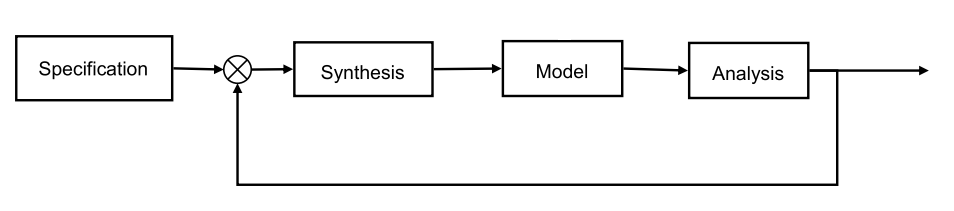
\includegraphics[width=0.9\linewidth]{images/PDPProcess.png}
		\caption{Product Development Process (PDP) (Source: Stolt~\cite{Stolt2008})}
		\label{fig:introduction:PDPProcess}
	\end{figure}
	
	\bigskip
	
Figure \ref{fig:introduction:PDPProcess} shows stages of PDP as presented by Stolt~\cite{Stolt2008}. It starts with ``Specification'' stage where the product requirements are studied, prioritized and are turned into concrete specifications. At ``Synthesis'' stage, various alternatives to address the specifications are evaluated. The most satisfactory alternative is designed at ``Model'' stage. Finally the designed model is evaluated against the specifications at the `'Analysis'' stage. If the analysis results are not satisfactory, then the process is iterated from ``Synthesis'' stage again, until a satisfactory product is arrived at.

PDP can be made more efficient either by reducing number of iterations or by reducing the time needed for each iteration, i.e. the time needed for the design and analysis of the product.
In past, before advent of computers, the design was done by manual calculations, sketches, etc., whereas the analysis was performed by testing physical prototypes of the product. In modern times, Computer-aided Design (CAD) applications are used extensively for design, whereas Computer-aided Engineering (CAE) applications are used for testing \& simulation of the products, virtually. Design calculations provide shape and size of the product. These shapes are modeled in CAD using various operations, such as extruding a sketch, revolve, fillet, etc. These modeling operations are known as features. The resultant CAD models are used for various downstream applications such as Computer-aided Manufacturing (CAM), visualizations, CAE, etc. In CAE, a CAD model is analyzed by decomposing it into mesh of elements, applying loads and boundary conditions and then solving the mesh for parameters such as stress, strain, displacements, etc. Thus, CAD-CAE process is a core stage of the modern PDP process and making it more efficient is key to reduce the Time to Market.

%
%Evolution of the PDP can be broadly classified into two eras, the pre-computers era and the computer era.  In the pre-computers era, calculations were done on paper, and prototypes were tested physically. This process was iterated till the design was satisfactory. 
%
%In the computer era, the PDP also goes through similar iterations, but the difference is that many of its sub-processes are handled with the help of computers. With increasing availability of vast and cheaper computational power, it has become imperative to leverage it for the core of PDP i.e. Design-Analysis, via approaches known as Computer-aided Design(CAD) and Computer-aided Engineering(CAE). Computers help in getting product design(CAD)  and its virtual validation(CAE), not just faster, but allow much needed iterations in far lesser costs than the physical counterparts. 

\section{CAD-CAE Process} \label{sec:intro:cadcae}

\todo{Review comments: Change this subsection to section. Either give complete description of CAD-CAE and to end process ow within this section add subsections pertaining to different steps in CAD-CAE product design cycle. [DONE]}

One of the critical aspect of the CAD-CAE process is the transformation of CAD model to CAE model. CAD models are often highly detailed, as they need to have information needed by various downstream applications. For CAE, many such details are not needed, because they add to the complexities in mesh generation and demand more computational power-time, for analysis. Removing such details and simplifying the CAD model is a necessary transformation and is a significant portion of preprocessing done to prepare the CAE model. This pre-processing is often not automatic and straightforward, but time consuming, manual and tedious.
%CAE offers virtual analysis of the product without building any physical prototype.  Even though the result fidelities are usually not as satisfying as the physical  prototyping experiments, CAE analysis is quick and often cost effective validation method. It helps designers understand the physical behaviors of the product, evaluate alternatives, perform experiments, do iterations and make decisions before committing the designed products to manufacturing.   So, although CAE does not fully \replaced{avoid }{takeaway} the necessity to build the physical models, but it can vastly reduce their number of iterations, thereby saving the cost and time. Due to such substantial advantages, industry \replaced{strongly needs }{desires nothing less than } a fully automated and reliable analysis process, but the current CAE systems are far from achieving this goal. The main reason is the presence of  different purposes of CAD-CAE data. CAD models are far more detailed than what is needed by CAE. This transformation from CAD model to CAE model is often manual and tedious process. 
\replaced{Thus there is a need to address these problems by a robust and automated simplification process}{To alleviate these lacunae, D. H. Brown Associate report   claims that  the system that would possibly do robust and automated CAD-CAE process would incorporate feature information to create more intelligent analysis models}~\cite{Halpern1997}. 
%CAD model, as mentioned before, being a generic input to various downstream applications, typically contains lots of details, some of which are irrelevant to CAE.  The unnecessary details add to the complexities in mesh generation, and demand more computational power-time for a relatively smaller gain in the accuracy of the results\cite{Thakur2009}. Also, the complex models may often lead to ill-conditioned matrices and hence working with non-simplified complex models may produce inaccurate results\cite{Saad2003}. Hence, simply utilizing more powerful computers will not solve the problem associated with the highly complex models. CAD models are, thus, simplified before sending them to CAE analysis. This transformation is known as ``Model Simplification''.  Although the Model Simplification significantly improves the analysis time, the deviation from the original shape, does introduce some error. Whenever, the gain in computation outweighs the error, model simplification is used. 


	\bigskip
	
	\begin{figure} [!h]
		\centering
		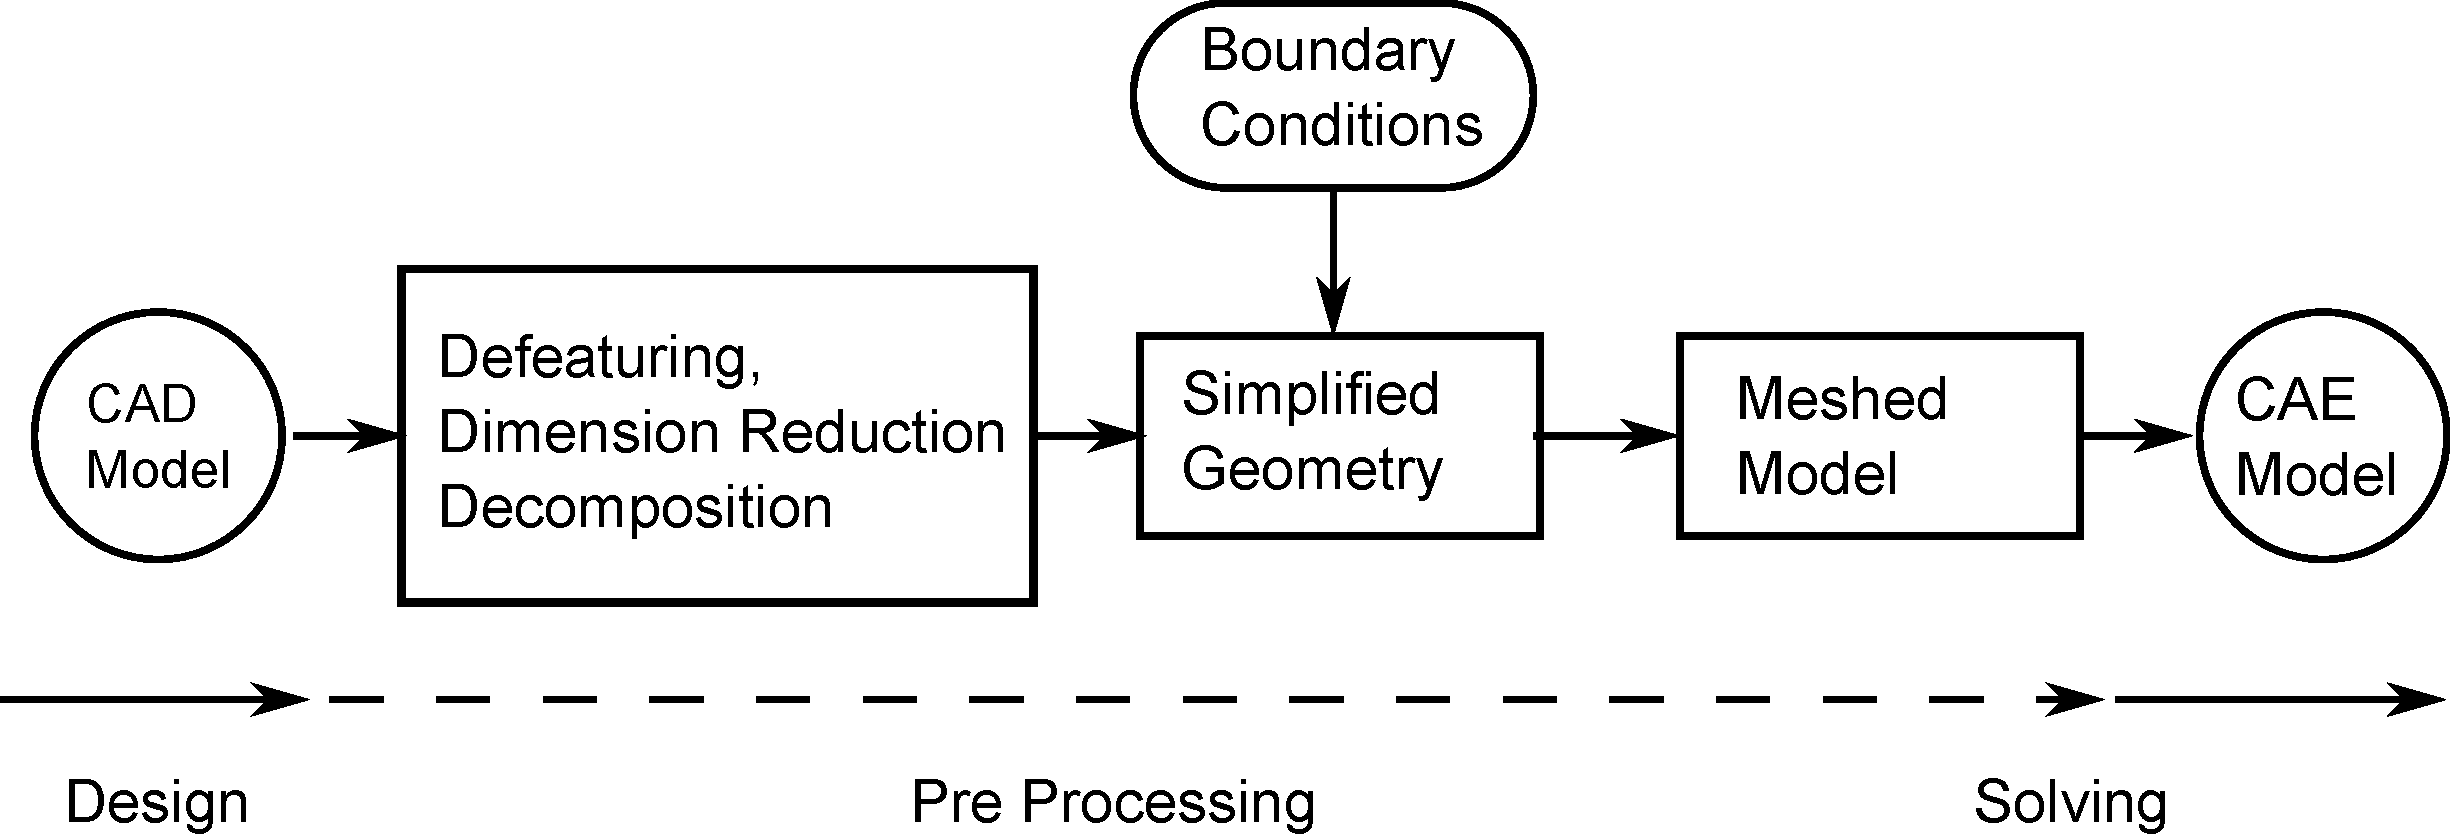
\includegraphics[width=0.9\linewidth]{images/CADCAEGeneralProcess.pdf}
		\caption{Computer-aided PDP (Source: Tierney~\cite{Tierney2013})}
		\label{fig:introduction:cadcaeworkflow}
	\end{figure}


	\bigskip
	
\todo{Review comment: Do not quote too many references here but provide a very high level overview of CAD CAE process. [REMOVED CITATIONS. REARRANGED]}

Figure \ref{fig:introduction:cadcaeworkflow} shows various stages which a CAD model undergoes to be ready for CAE analysis. Simplification, as shown in the first box, mainly consists of defeaturing and dimensions reduction. In defeaturing, irrelevant details are removed by removing corresponding features. Due to defeaturing, meshing is not unnecessarily dense and complicated around the irrelevant details. Thus defeatured model reduces number of elements, which correspond to lesser degrees of freedom (DoFs) of the mesh, thereby saving analysis time and resources substantially.  In dimension-reduction, shapes like slender-bar, thin-wall are transformed into their lower dimension representations such as curves and surfaces, respectively. Lower dimension representations are used for lower dimension element types such as beams or shell which have far lesser DoFs than the solid elements. Thus use of dimension reduction reduces analysis time and resources further.
% Once meshing is complete, loads and boundary conditions are applied. Based on the analysis type (static, dynamic, modal) further computations are carried out. Output results are presented either in the form of reports or visualizations. If this analysis finds certain weaknesses, design changes are suggested, which, when done, the analysis iteration is carried out once more. This process repeats till satisfactory model is arrived at.

Dimension reduction transformation is widely used in CAE analysis of thin-walled parts, such as sheet metal and plastic products.  CAD models of these parts are transformed into a representative surface known as ``Midsurface''. It is a surface lying midway of a thin-walled CAD model and mimicking its shape.  Getting a correct midsurface is critical to CAE analysis of thin-walled parts.
%
%For sheet-metal, plastic products (generically classified as `thin-walled'),  a quick and fairly accurate CAE analysis is possible by idealizing their CAD solid models to the equivalent surface representation called ``Midsurface'' (Note: `Midsurface', `Mid-plane' and  `Medial Object' are used synonymously in this work, unless specified otherwise). It can be envisaged as a surface lying midway of a thin-walled solid, and mimicking its shape.
%Despite an extensive research and high commercial demand, there is still a significant disconnect is observed between CAD and CAE. It is mainly due to lack of automated, robust defeaturing and dimension-reduction approaches\cite{Nolan2015}.  The present research focuses on the dimension-reduction by developing an automatic, deterministic and generic approach for the computation of a well-connected midsurface, along with associated defeaturing, for thin-walled CAD models.
	
\section{Midsurface for CAE Analysis of Thin-walled Parts} \label{sec:intro:cadcae}

CAE analysis of the thin-walled parts using 3D solid mesh elements such a Hexahedral or Tetrahedral, is expensive in terms of computing resources and time taken. 2D surface mesh elements such as Shell, are preferred as they give reasonably accurate analysis results, while requiring far lesser computational resources and time~\cite{Elangovan2012}.  Shell elements need midsurface and thickness values for their definition and usage. Thus, midsurface is the most widely used representation of thin-walled parts for CAE analysis.

The midsurface is expected to be ``well-connected'' (patches form a continuous surface) and resembles shape of the input CAD model (more details at Fig.~\ref{fig:introduction:midsurfaceexptations}).
 
 Most midsurface generation approaches are based on the final shape of the CAD model. It is typically represented by a data structure known as Boundary Representation (Brep). In Brep, a solid shape is represented by a set of connected faces to form a closed volume. Midsurface is computed either by applying geometric transformations or by using heuristic rules on Brep. 
 
Face pairing is one of the most popular midsurface computation method based on Brep. Faces opposite each other are detected to form face-pairs. Each face pair computes an equidistant surface in the middle, called midsurface patch. These patches are then, either extended or trimmed to join at a common edge to form a well-connected midsurface. Although this approach works well on simple, academic models, it often fails in case of real-life, complex models. Failures are in the form of gaps between patches, overlaps, midsurface not lying midway, etc.  Thus, minimizing the failures and devising a robust approach to compute a well-connected midsurface is critical to the CAD-CAE process of thin-walled parts.
 
% In complex Brep shapes it is challenging to find appropriate face pairs and to join midsurface patches correctly. Instead of the final Brep shape, few approaches use the model construction information, in the form of features, to compute the midsurface~\cite{Robinson2006}. This feature-based approach is promising as at each feature step in the construction, shapes are relatively simpler than the final model shape.
% 
% So, they do not leverage feature information available in modern feature based CAD applications. The reasons are multi-fold.  Since beginning, CAD and CAE products evolved separately, by different companies. Interoperability between them was through neutral B-rep formats. It was done so for avoiding export of  proprietary design intent information in the form of features. 
% \deleted{Now, with far more integrated CAD-CAE environments, and access of features through APIs it is possible to leverage feature-information in CAE, as demonstrated in the present research for generating midsurface.} 
% 
% In recent times, CAD systems have started exposing the feature information through Application Programming Interfaces (API) for better support to 3rd party applications. Now it is possible to build own algorithms, as this research does, leveraging the feature information as it is a  rich source of part creation information. It can have advantages over current 
%midsurface generation algorithms, which are largely based on rudimentary heuristics and lack appropriate topological validation. The work presented in this thesis aims at effectively utilizing feature information for simplification of model as well as the feature tree so that the part model can be represented by a very minimal set of features and complexity of midsurface generation problem is drastically reduced. Further midsurface connections are resolved by a very generic algorithms that cover a wide range of connectivity problems. The research further adds apt topological validation to correlate CAD part model and corresponding midsurface.

\todo{Review comment: I don't think this type of citation (footnotes) fits into specified format. [REMOVED FOOTNOTES]}
\todo{Review comment: You only finished till simplification what are the further steps till CAE analysis is done and how that info is used? [ADDED NOTES FOR FURTHER CAE STEPS]}
\todo{Review comment: Once you have introduced term midsurface in CAD CAE process, no need to define it here. Only talk about why midsurface are still critical for thin walled parts. [DONE]}
\todo{Review comment: Change heading of this paragraph. [DONE. MOVED SANDIA REPORT PARA TO PREVIOUS SECTION]}	
\todo{[ADDED FOLLOWING PARAGRAPH AS PER SUGGESTION. NOT USED `MIDCURVE' AS NOT DEFINED SO FAR]} 

\section{Motivation of Research}

 Midsurface is the most suitable representation for the CAE analysis of thin-walled parts' CAD models. 
 A Sandia report~\cite{Ming2012} states that, for the complex engineering models, their simplification amounts to about 60\% of the overall analysis time, whereas the mesh generation consumes about 20\% and solving the actual problem takes about 20\%.  In the shipping industry, more than 80\% of CAE engineer's time is spent on modeling dimensionally reduced entities~\cite{Austreng2007}. Automex~\cite{Automex} observed that the complexity involved in generating midsurfaces takes about 70 to 90\% of the pre-processing time. % In case of crash simulation components, this time can go up to 14 days.
Thus,  computing well-connected midsurface is highly critical to the industry.

%So, even in this age of scalable and near-infinite computing power, it is still desirable to have  this idealized representation, instead of just pouring millions of 3D elements\cite{Abbey2013}. With far lesser nodes and degrees of freedom one is able to run more design iterations quickly.  Thus, midsurface is the most suitable idealization for the analysis of thin-walled parts.   Because of this  advantage,  having an automatic, deterministic and generic method for computing well-connected midsurface is critical to the  industry.
Despite extensive research, many midsurface computation approaches fail to generate a well-connected midsurface, especially for the complex part shapes. Correcting the errors is mostly a manual, tedious and highly time-consuming task, requiring hours to days. This correction time can be nearly equivalent to the time it can take to create the midsurface manually from scratch~\cite{Stolt2006}. 

Thus, looking at the criticality, the present research focuses on design and implementation of a system to generate a well-connected midsurface for thin-walled parts.

\section{Scope of the Work}  \label{sec:litsurvey:rscope}

\todo{TODO: RE-CHECK THE MEANING OF THE PARAGRAPH}

%% As explained in Section \ref{sec:intro:cadcae}, modern PDP process heavily depends on CAE for validation of the CAD models. Validation is for assessing strength, studying interaction with fluids, checking abilities to withstand heat-temperature, understanding model behavior, etc.  

Thin-walled parts are present in a variety of domains, such as plastics, sheet metal, machined components, etc. They are either constant thickness parts such as in sheet metal domain, or variable thickness parts, as in plastics domain.  D. W. Brown Report~\cite{Halpern1997} suggests that sheet metal parts is one of the most widely used sub-category, with approximately 40\% share amongst the manufacturing processes. They are found in a wide variety of applications such automobile, aircraft, shipbuilding, consumer products, electronic equipments, etc.  


\bigskip

\def \myfigstairspcolumnwidth{0.21}

\begin{figure}[h!]
\centering  
\subfloat[Harvester]{\label{fig:introduction:harvester}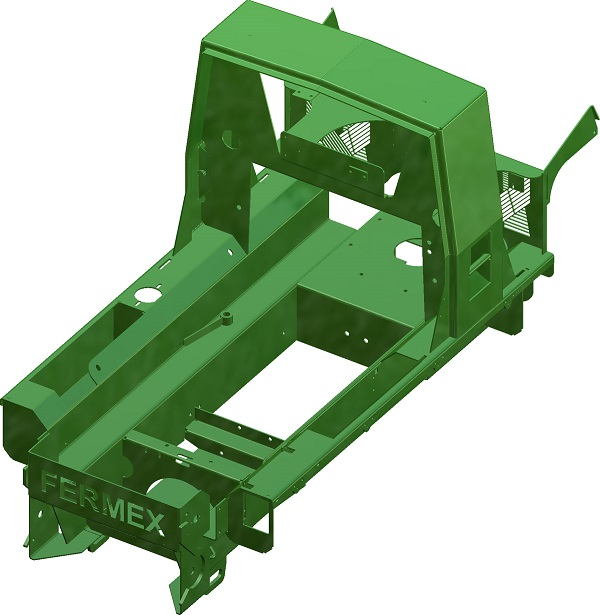
\includegraphics[width=0.16\linewidth]{images/SheetMetal_isd_cad_blech_vermeer}} \quad
\subfloat[Enclosure]{\label{fig:introduction:enclosure}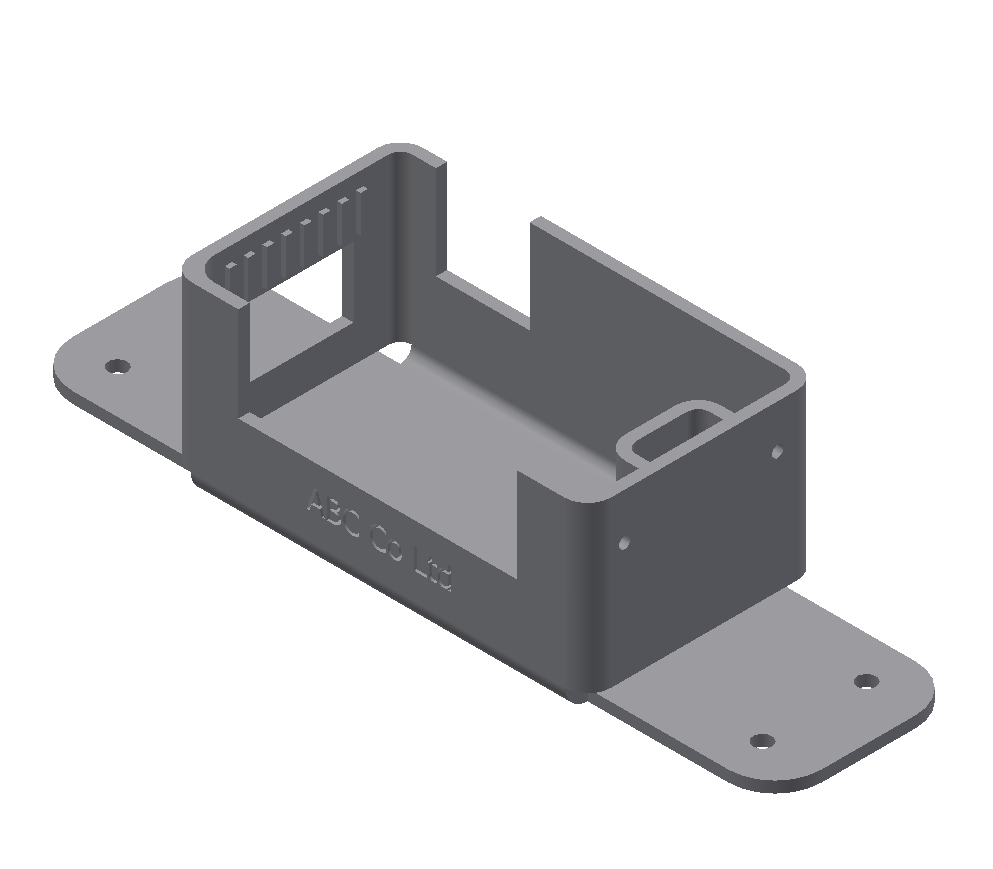
\includegraphics[width=\myfigstairspcolumnwidth\linewidth]{images/SheetMetal_Medium_Enclosure_OriginalPart}} \quad
\subfloat[Bracket]{\label{fig:introduction:bracket}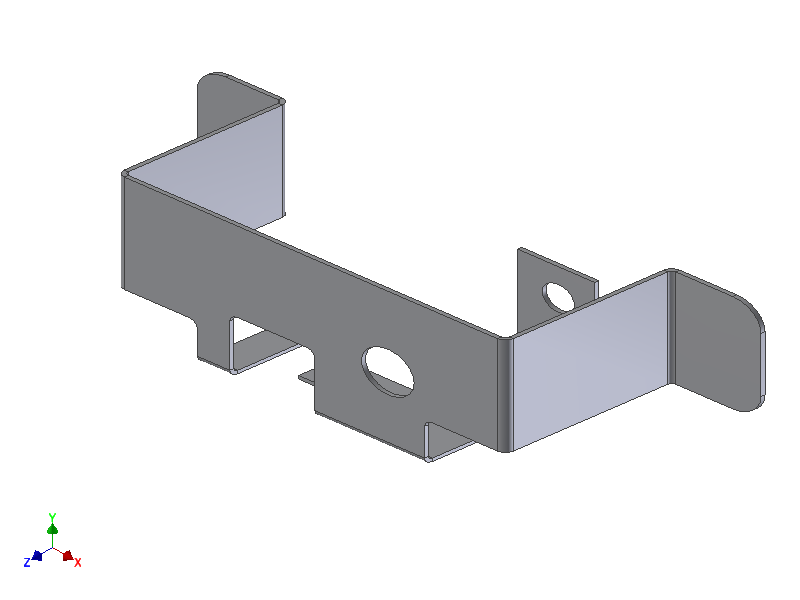
\includegraphics[width=\myfigstairspcolumnwidth\linewidth]{images/SheetMetal_Simple_UBracket_OriginalPart}}   \quad
\subfloat[Duct]{\label{fig:introduction:duct}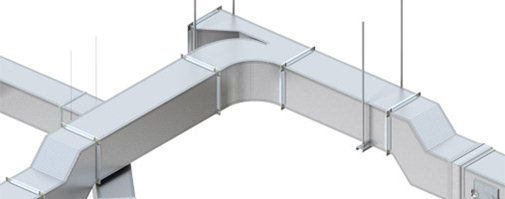
\includegraphics[width=\myfigstairspcolumnwidth\linewidth]{images/SheetMetal_KDuct-Main-Render}}
\caption{Variety of Sheet Metal Parts}
\label{fig:introduction:sheetmetalsamples}
\end{figure}


\bigskip

\todo{Review comment: Can computer casing be replaced by one of the case study parts? Use stapler part. [DONE]}

Figure \ref{fig:introduction:sheetmetalsamples} shows some of the sheet metal parts, such as an agricultural harvester frame~\cite{harvester}, an enclosure commonly used in electrical systems, a bracket found in mechanical systems and HVAC ducting. Looking at the range of the sheet metal products, any improvement in their CAE analysis will have a significant impact on the product development process of all these domains. \replaced{Hence the domain of sheet metal parts is being considered in the proposed research. }{So, the present research plans to focus on getting the most crucial sub-process of the CAE prepossessing right, i.e. generating a better midsurface.}

Thus, the present research work focuses on proposing an approach to generate a well connected midsurface, which will improve results of CAE analysis of sheet metal CAD models. The approach is elaborated in details in the following chapters of this thesis.

\section{Organization of the Thesis}

The subsequent organization of the thesis is as follows:

\begin{itemize}[label={},leftmargin=*]

\item Chapter  \ref{ch:Survey} reviews the relevant literature on the traditional midsurface generation approaches along with auxiliary approaches such as defeaturing and decomposition. Specific issues and limitations of these approaches are highlighted. The chapter concludes by outlining objectives of the present research work.

\item Chapter \ref{ch:Proposal} presents an overview of the proposed system to generate well-connected midsurface of sheet metal feature based CAD model. It describes major modules involved with respect to their functional capabilities and interrelationships.

\item Chapter \ref{ch:Defeaturing} presents at length the algorithms for defeaturing.  It initially outlines the phases and then subsequently presents in details the methodology and the algorithms to generate the simplified feature based CAD model.

\item Chapter \ref{ch:Abstraction} presents the algorithms to transform the sheet metal features to a generalized finite set of features. Such generalized feature based model aids in reducing the complexity of the algorithms.

\item Chapter \ref{ch:Midsurface} \replaced{details out various strategies to generate midcurves, midsurface patches and dedicated algorithms to join them.}{reports at length various steps the abstracted model goes through, such as cellular decomposition, midsurface patch generation, patch joining, etc. Towards the end of this chapter, various characteristic shapes are used to demonstrated the efficacy of the algorithms.}

\item Chapter \ref{ch:Validation} presents a newly proposed methodology for validating midsurface based on topological considerations.

\item Chapter \ref{ch:Testing} demonstrates the capabilities of the proposed system for generating quality midsurface with reference to typical model case studies.

\item Chapter \ref{ch:Conclusions} summarizes the research work highlighting the major contributions and outlines direction for the future work.
\end{itemize}





% ----------------------------------------------------------------------------------------------------
\chapter{Literature Survey} \label{ch:Survey}
\section{Introduction} \label{sec:survey:intro}

This chapter presents, in details, a review of relevant literature on reported approaches for generation of midsurface. These approaches have been critically examined and compared to highlight their specific advantages and limitations. The chapter concludes by enumerating the objectives of the present research work.

\todo{Review comment: Why Simplification is right in the beginning? Instead provide reported definition of midsurfaces, figures for what they are used \& how and why this has been topic of research. [REMOVED MODEL SIMPLIFICATION RELATED CONTENT. PUTTING MIDSURFACE RELATED]}

Midsurface is the most widely used surface representation of thin-walled CAD solid model for CAE analysis. 

%%\bigskip

		\begin{figure} [!h]
		\centering
		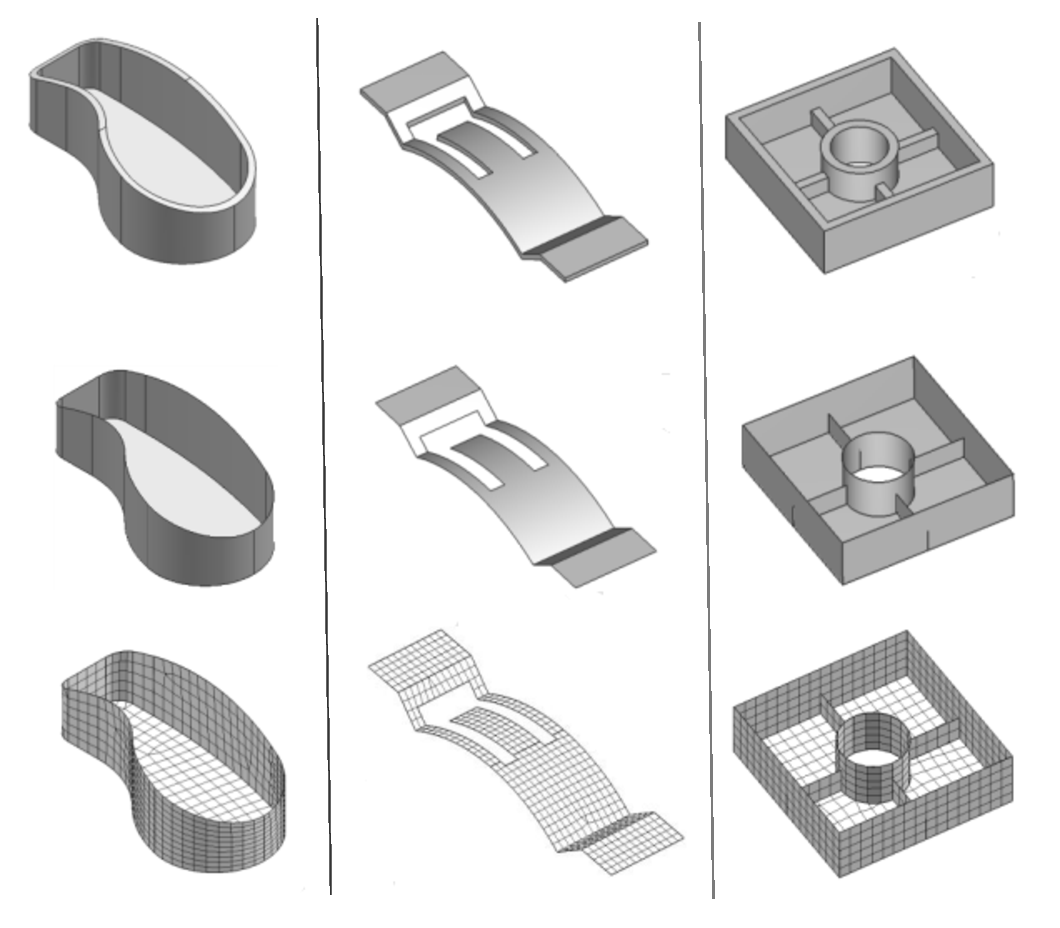
\includegraphics[width=0.75\linewidth]{images/WooMidsurfaces.pdf}
		\caption{Thin-walled Models, Midsurfaces, Meshes (Source: Woo~\cite{Woo2013})}
		\label{fig:introduction:woomids}
	\end{figure}
	
%%\bigskip

Figure~\ref{fig:introduction:woomids} shows 3 thin-walled CAD models in the first row. The second row shows their corresponding midsurface representations. The third row shows shell meshing applied on the midsurfaces for CAE analysis. Midsurface, in different forms, such as medial objects, mid-planes, etc., are being researched for decades. Still, there is no robust, fully automated method for its computation. The reason for this unsolved problem is that there is no single, formal definition of midsurface~\cite{Ramanathan2004}. Different applications which use midsurface have different expectations about its shape, especially at the connection points. Figure~\ref{fig:introduction:midsurfaceexptations} shows how midsurface expectation varies~\cite{Woo2013}.


%%\bigskip

\def \myfigstairspcolumnwidth{0.22}

\begin{figure}[h!]
\centering     %%% not \center
\subfloat[Model]{\label{fig:introduction:stairsmodel}
\includegraphics[width=\myfigstairspcolumnwidth\linewidth]{images/Stairs_part_2.pdf}} \quad
\subfloat[Gradual]{\label{fig:introduction:stairsfl}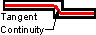
\includegraphics[width=\myfigstairspcolumnwidth\linewidth]{images/Stairs_follows_2.pdf}}  \quad
\subfloat[Mimicking]{\label{fig:introduction:stairsmk}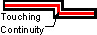
\includegraphics[width=\myfigstairspcolumnwidth\linewidth]{images/Stairs_mimic_2.pdf}}   \quad
\subfloat[Disjoint]{\label{fig:introduction:stairsseparate}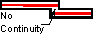
\includegraphics[width=\myfigstairspcolumnwidth\linewidth]{images/Stairs_separate_2.pdf}}
\caption{Midsurface Configurations for a Given Shape}
\label{fig:introduction:midsurfaceexptations}
\end{figure}

%%\bigskip

Figure~\ref{fig:introduction:stairsmodel} shows a step shaped thin-walled solid CAD model represented schematically as a 2D shape. Figure ~\ref{fig:introduction:stairsfl} shows two midsurface patches being joined in a gradual manner, known as  $G_1$  i.e. tangent geometric continuity. Such midsurface is preferred for CAE analysis. Figure ~\ref{fig:introduction:stairsmk} shows a planar patch being added to join the two midsurface patches. This midsurface mimics the original model exactly and is best suited for  shape matching or retrieval kind of applications where exact representation is preferred. Figure ~\ref{fig:introduction:stairsseparate} shows midsurface patches disconnected and such output can be used where the disconnect needs to be highlighted. A closer observation will reveal that all the output midsurfaces, shown in Figure~\ref{fig:introduction:midsurfaceexptations}, vary in the continuities between midsurface patches at the connections. These continuities are of 3 types: touching ($G_0$), tangent ($G_1$) and curvature ($G_2$ ). Continuities shown in the in Figure~\ref{fig:introduction:midsurfaceexptations} are of  types $G_1,G_0,0$ respectively.  The present research works aims at producing midsurface with $G_0$ continuity.

Although there is no single, formal definition of the midsurface, some researchers have specified it semi-formally, as below:

\begin{mydef}\label{def:midsram}
Mid-surface is an aggregation of surface patches (where each patch corresponds to a pair of non-adjacent surface patches (faces) in the object that are closest to each other) that form a closed and connected set and that satisfy homotopy (Ramanathan~\cite{Ramanathan2004}).
\end{mydef}

\begin{mydef}\label{def:midsrez}
Midsurface is expressed as contiguous flow of the input solid's shape (Rezayat ~\cite{Rezayat1996}).
\end{mydef}

Primary usage of midsurface is in the CAE analysis of thin-walled parts models for placing surface elements such as ``shell'' elements.
%The present research work proposes mimicking, i.e. $G_0$ continuity output (Figure~\ref{fig:introduction:stairsmk}) as it represents the input shape faithfully. The proposed method can cater to other variations as well by incorporating with additional connection rules. These enhancements are for the future scope.  So, the primary objective of the present research work is to devise an approach to computed a well-connected midsurface mimicking the input model faithfully, in both, geometry and topology.
%%In CAE, detailed CAD model is not used as is (Section~\ref{sec:intro:cadcae}), but it is preprocessed by `Model Simplification'~\cite{DengBrittonLamTorMa2002,Lee2005,Lee2009,Lam} (Figure~\ref{fig:introduction:ModelSimplification}).
%%
%%%%\bigskip
%%
%%	\begin{figure} [!h]
%%		\centering
%%		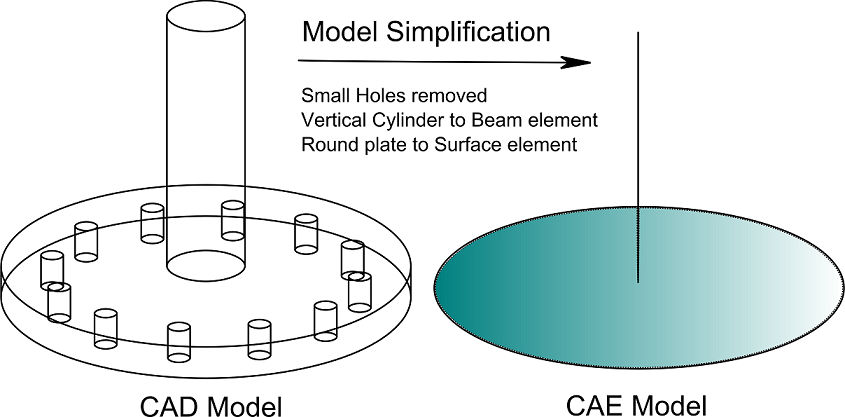
\includegraphics[width=0.6\linewidth]{images/ModelSimplification.png}
%%		\caption{Model Simplification}
%%		\label{fig:introduction:ModelSimplification}
%%	\end{figure}
%%
%%%%\bigskip
%%
%%	Model Simplification, according to Hamri~\cite{Hamri2005}, is classified into:
%%	\begin{itemize}[noitemsep,topsep=2pt,parsep=2pt,partopsep=2pt]
%%	\item  \textbf{Skin Details}: Removal does not change 3D manifold property, like fillets, chamfer, etc.
%%	\item  \textbf{Topological Details}: Removal changes solid model topology, like, through holes etc.
%%	\item  \textbf{Dimensional Details}: Idealization, such as lines for long slender bar, midsurface for plates.
%%	\item  \textbf{Simplification Features}: User defined features to be removed.
%%	\end{itemize}
%%
%%Similarly, Model Simplification, according to Dabke~\cite{Dabke1994}, can be classified into two sub-processes, namely, Global and Element Idealization. The global idealization deals with suppressing irrelevant features and takes advantage of the symmetry to analyze only a portion of the model (also known as ``Defeaturing'' \footnote{``Defeaturing'' and ``Simplification'' have  been used interchangeably in this work, unless specified otherwise. ``Model Simplification'' is far more encompassing term, having both defeaturing and dimension-reduction, along with a few other techniques.}).  In the element idealization, shapes like slender-bar, thin-wall are converted into lower dimension geometries like midsurface. 
These elements are considered superior over solid elements, such as hex (Hexahedral) or tet (Tetrahedral), as they are computationally faster and still deliver fairly accurate analysis results. 
%In many applications, reducing the dimensions of CAD models is beneficial. For example, consider a thin plate of uniform thickness. If we model this plate using shell elements (2D surface), there will be a negligible effect on the accuracy of the CAE analysis but the computational time will reduce dramatically. Hence, dimensional reduction is studied by the physics-based simulation community (especially finite element analysts) for model simplification purposes~\cite{Thakur2009}.
%Shell elements best represent parts whose walls are `much' thinner than their typical feature size~\cite{Subrahmanyam2012}. 
%Although criterion for ``thinness'' depends on the application domain, $L/t > 20$ can be a generic consideration~\cite{Cosmos2006}.  
%%\bigskip

\begin{figure} [!h]
\centering
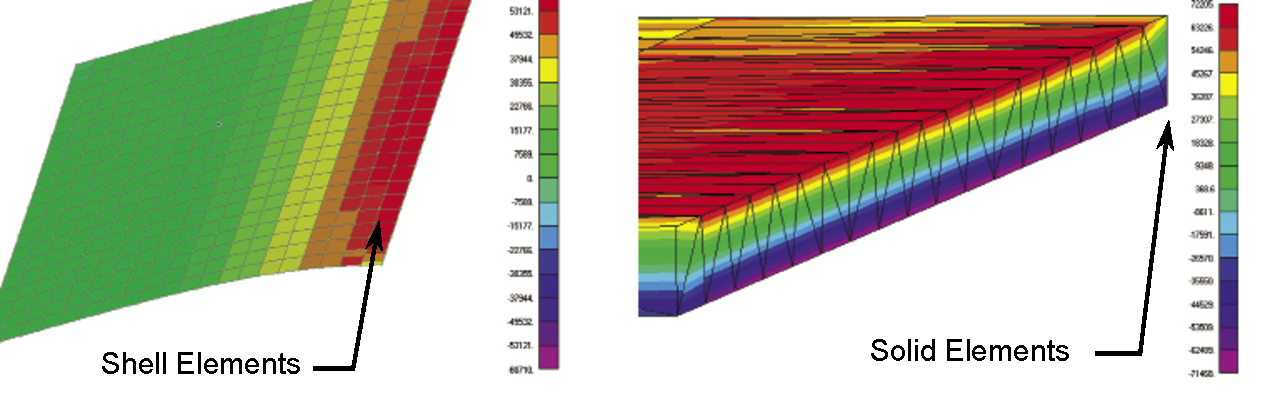
\includegraphics[width=\linewidth]{images/solidshelldesk_1.pdf}
\caption{Comparison of CAE Analysis with Solid/Shell Elements (Source: Digital Eng~\cite{Abbey2013})}
\label{fig:introduction:solidshell}
\end{figure}
	
%%\bigskip

Figure~\ref{fig:introduction:solidshell}  shows CAE analysis results plots of a simple plate structure. The first figure shows the result with shell elements and the second shows with tet elements. Shell elements give peak bending stress and tip deflection, very close to the theoretical calculations. Tet elements give good deflection values, but poor stress values. The tet mesh is only one element deep. To get accurate stress values, the tet element mesh needs to be at least three elements deep. To avoid the high aspect ratios, in a sample case this may drive the tet element count up towards 1 million, vs. 400 for the shell elements mesh~\cite{Abbey2013}. Thus shell element mesh is far superior in analyzing thin-walled models. A well-connected midsurface is a critical requirement for placing the shell elements.

In some cases, even for relatively thick portions, analysts use midsurface as it gives them the flexibility to play with the thickness which is not possible in case of 3D elements. While solid elements could be used for thin-walled parts, they are inefficient since many more solid elements are required to capture the same response a shell mesh can. At worst, if too few solid elements are used in a bending dominant condition, the results may appear to be correct but could be overly stiff. So, for thin-walled parts shell elements on midsurface are preferred~\cite{Cosmos2006}.
	
Although there are many approaches to generate the midsurface, following section details a representative, traditional and one of the most popular approach of generating midsurface.
	
\section{Traditional Approach for Generating Midsurface}

\todo{Review comment: Get into these section with 1/2 lines as intro. Then enumerate typical steps for traditional approach and then start commentary on reported research on those steps. [DONE]}

Midsurface generation is one of the sub-types of dimension reduction process. It, along with defeaturing, forms overall ``Model Simplification'' process, which is performed during preprocessing of CAD model for CAE analysis. Traditionally, both, defeaturing and dimension reduction, are done together, one after another.

%%Approaches to generate midsurface have been part of research and commercial applications for decades. As seen in Section~\ref{sec:intro:cadcae}, these dimension reduction approaches are part of a larger process called ``Model Simplification''. Approaches for Model Simplification vary substantially, depending on the input type, such as faceted mesh model, Brep CAD model, feature-based CAD model, etc.\cite{Lam1992, Thakur2009, Yogesh2010}. 

\todo{Review comment: Can you not combine model simplification \& defeaturing?. [MODEL SIMPLIFICATION ACTUALLY COMBINES DEFEATURING AND DIMENSION REDUCTION IE MIDSURFACE. THIS PARAGRAPH IS ABOUT REMOVING IRRELEVANT FEATURES SO NAMED AS DEFEATURING]}

Figure~\ref{fig:introduction:hamdimids} shows a representative approach, a schematic outline of overall model simplification process presented by Hamdi~\cite{Hamdi2005, Hamdi2007, Hamdi2009, Hamdi2010, Hamdi2012}.
%% with following phases:
%%
%%\begin{enumerate}[noitemsep,topsep=2pt,parsep=2pt,partopsep=2pt]
%%\item  Identification of features in the input Brep or mesh model.
%%\item Identification of features to be removed, based on heuristic rules.
%%\item Generation of midsurface patches and then joining them together.
%%\item Validation of the output midsurface.
%%\end{enumerate}

%%\bigskip

	\begin{figure} [!h]
		\centering
		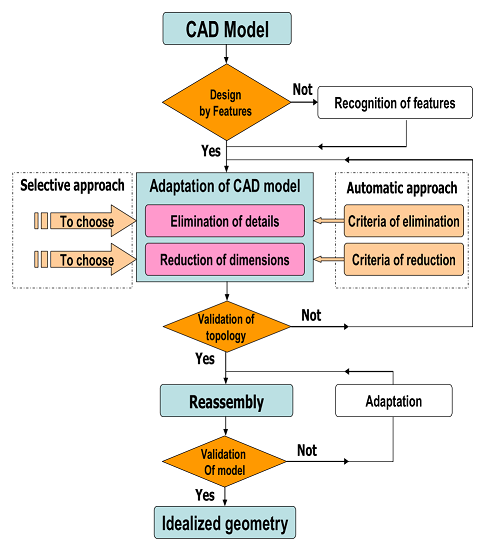
\includegraphics[width=0.75\linewidth]{images/BlockDiagramSampleHamdi}
		\caption{Model Simplification Approach (Source: Hamdi~\cite{Hamdi2005})}
		\label{fig:introduction:hamdimids}
	\end{figure} 

%%\bigskip

CAD model is the input to this approach. It can be either feature based (denoted as ``Design by Features'' in~\ref{fig:introduction:hamdimids}) or non-feature based (i.e. Brep model). If it is Brep model, then it undergoes feature recognition process to identify features, thereby making it `feature-based CAD model'.  At the ``Model Simplification'' stage (called ``Adaption of CAD model'' in Figure~\ref{fig:introduction:hamdimids})), both defeaturing (called ``Elimination of details'') and midsurface generation (called ``Reduction of dimensions'') are performed together, one after another. In defeaturing, irrelevant features are removed, with `irrelevance' specified by `Criteria of elimination'. In dimension-reduction midsurface is generated, with `thin-walled' portions selected based on `Criteria of reduction'. The output midsurface is validated and if successful, (shown as as `Idealized geometry') sent to further downstream applications.

Figure~\ref{fig:introduction:tradmidsurfgen} shows another traditional approach with more details of actual midsurface generation process. The input CAD model (called ``Solid Model'') is defeatured in the second stage (called ``Simplification''). Here, irrelevant features such as small fillets, chamfers, etc. are removed. Midsurface computation is done using Face pairing approach. The  third stage (called ``Pair Detection'') shows how opposite faces are detected and their face pairs are formed. In the fourth stage, midsurface patches are generated. Patches are then trimmed or extended to meet at common edge. The midsurface patches are then stitched to form the final, well-connected, midsurface model.

%%\bigskip

	\begin{figure} [!h]
		\centering
		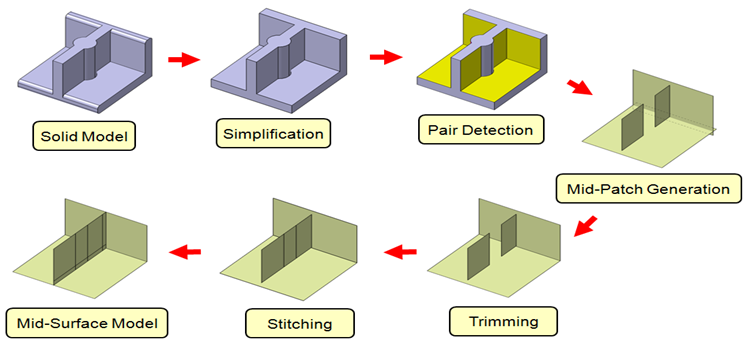
\includegraphics[width=0.9\linewidth]{images/MidsurfaceProposedApproach}
		\caption{Traditional Midsurface Generation Approach (Source: Sheen~\cite{Sheen2005})}
		\label{fig:introduction:tradmidsurfgen}
	\end{figure} 

%%\bigskip

Both traditional approaches show the sequential execution of defeaturing and midsurface generation, as part of model simplification process. Finally, the output midsurface is validated for correctness. The following sections detail the state of the art for all of these.

\section{CAD Model Defeaturing Approaches} \label{sec:survey:defeat}

Humans, while looking at an object, at the first glance perceive its overall, gross shape and then eventually look into more details as needed~\cite{LeeLee1998}. Gross shape is the principal shape that ``represents'' the given shape, but with far lesser features. In the context of CAD-CAE the gross shape is achieved by defeaturing. Defeaturing is the process of simplification of the shape, by removing small and irrelevant feature details,  based on certain predefined objectives or criteria. It is primarily used in CAE analysis where such simplified models lower the complexity of the finite element mesh and thus reduce the analysis time. It is also used in shape matching \& retrieval, fast visualization, hiding proprietary details, transmission across the network, etc. 

\todo{Review comments: What are refs? [REMOVED BOTH DEFINITIONS]} 

% \replaced{The present research}{This} work focuses on using defeaturing for finding the gross shape needed in the computation of well-connected midsurface. 	
	
%%Grossness depends on the size criteria or threshold. Details having sizes below the threshold are removed. With lesser irrelevant details on the input model, the generated midsurface becomes far more representative of the input model and is robust (any small change in the input model shape does not affect the output midsurface in any appreciable manner).
	
Traditionally, defeaturing has largely been a manual and tedious task. Small and irrelevant features are first recognized in the input mesh or Brep CAD model and are removed manually~\cite{BelazizBourasBrun2000}. Users view this task as too extensive and resort to recreate the necessary geometry than to simplify the existing one~\cite{Halpern1997, Abbey2013,Lam,Lee2005, Lee2009}.  
	
%In the \replaced{traditional }{current CAD-CAE applications, many} simplification methods recognize small, irrelevant features on a mesh or a solid body first, then remove them to get the simplified (called ``defeatured'')  model~\cite{}. 

\deleted{Instead, if a feature based CAD model is used as an input, then it has the advantage of the availability of ready features, so that the suppression and healing becomes relatively straightforward and robust. In such a feature based defeaturing method, the primary challenge is the identification of the suppressible features.
 In the past, the suppressibility used to be based on some insufficient criteria, like using full feature parameters, selecting all the negative features, etc. The objective of this work is to use far more accurate criteria and develop a computational method to automatically find the simplified geometry of a sheet metal part model which can be used for further computations such as the generation of the midsurface (more details in the Chapter~\ref{ch:Defeaturing}).} Feature-based defeaturing approaches can be classified as:

\begin{enumerate}[noitemsep,topsep=2pt,parsep=2pt,partopsep=2pt]
	\item CAD Model Defeaturing based on Feature Information.
	\item CAD Model Defeaturing based on Feature Recognition.
	\item CAD Model Defeaturing based on Decomposition.
\end{enumerate}

Following section elaborates theses approaches in details. \deleted{This research uses defeaturing of the feature based CAD model, using decomposition as well as feature data, thus their state-of-the-arts are presented below.} 

\todo{Review comments: Delete. [WITH THIS DELETION THE CONTINUITY IS GONE. RESTORE BACK?]}

\subsection{CAD Model Defeaturing Based on Feature Information}

Thakur et al.~\cite{Thakur2009} surveyed and classified various model simplification approaches into four categories, such as surface-based, volume-based, feature based, and dimension-reduction. First three categories are about defeaturing and the fourth is for midsurface generation. \added{From this survey it is observed that} most methods were based on the mesh and Brep model as the input, with very few based on the feature based CAD model. 

In feature-based CAD, model is built step by step using feature modeling operations. The history of modeling operations is represented in the form of feature tree.

%%\bigskip

	\begin{figure} [!h]
		\centering
		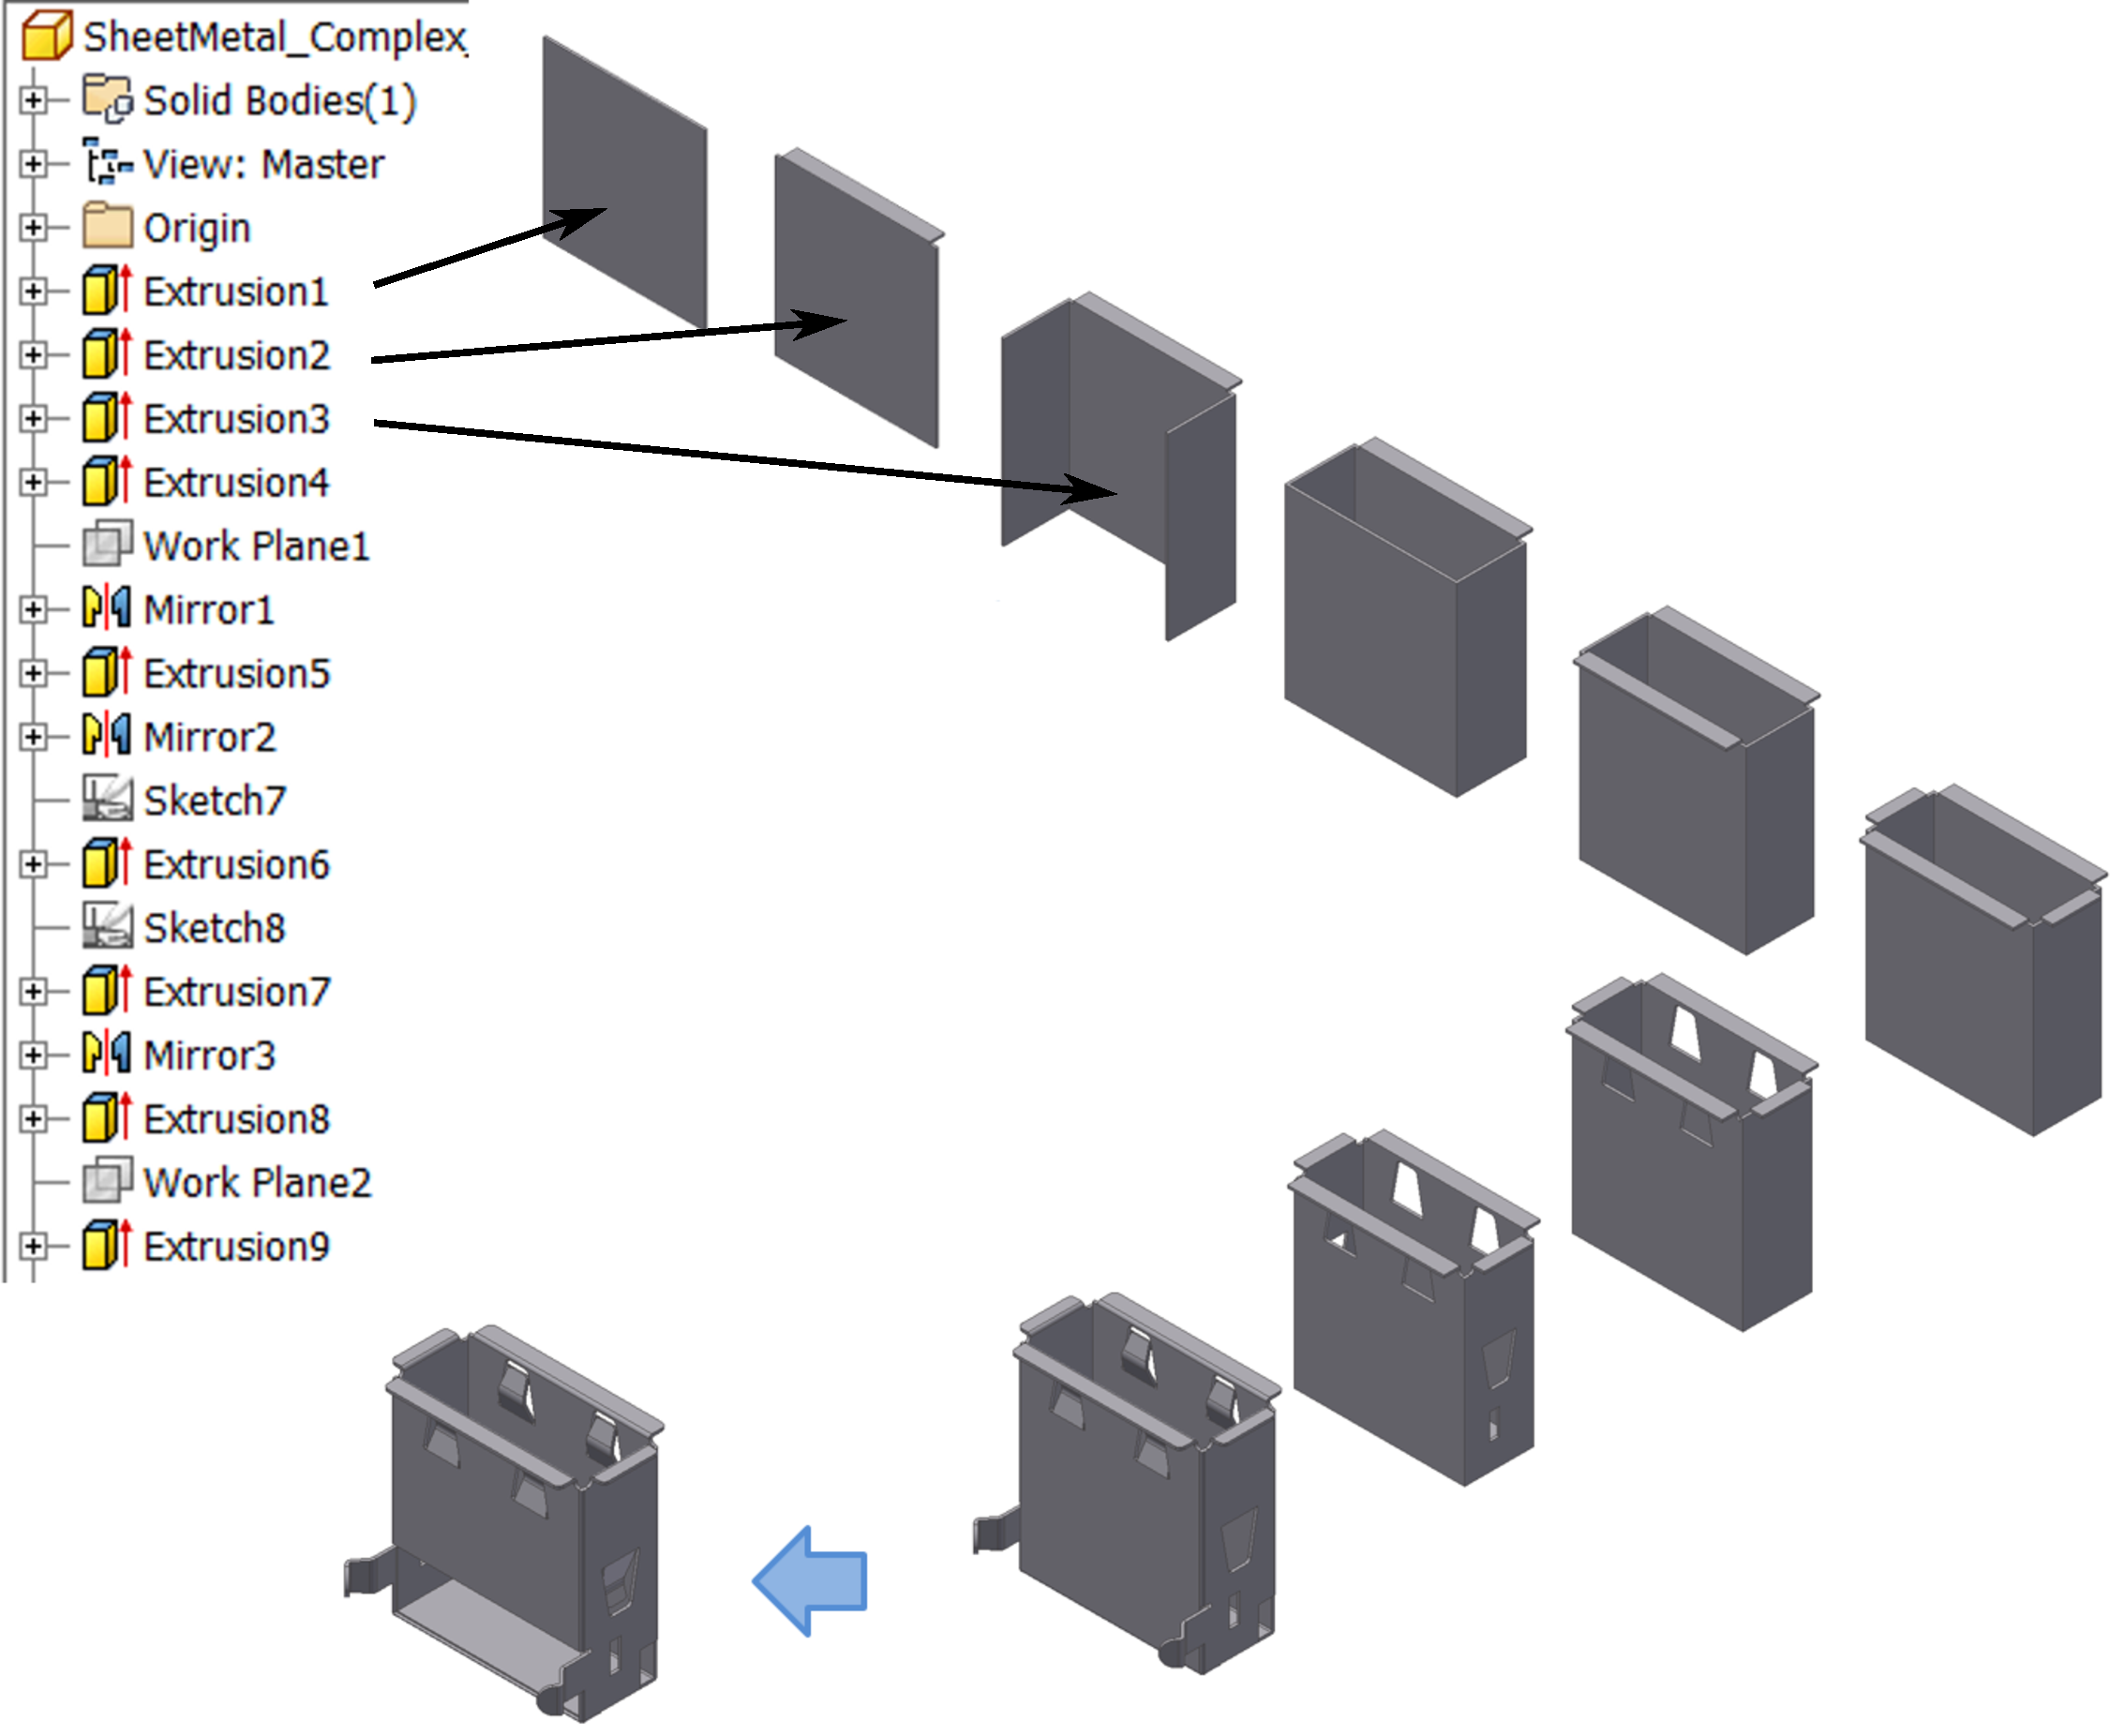
\includegraphics[width=0.75\linewidth]{images/usbfeaturetree_arrow.pdf}
		\caption{Construction of USB CAD Model by Features}
		\label{fig:introduction:usbtree}
	\end{figure} 

%%\bigskip

Figure~\ref{fig:introduction:usbtree} shows construction of a CAD model of a USB part using a variety of modeling features. At each stage, a new feature gets added to or subtracted from the model built till then. The feature tree is shown at the left. Feature based CAD model, internally builds the model in Brep format as well. So, the final shape, shown at the bottom can be exported in the Brep format. Non-feature based CAD models create Brep format directly and are not built using features. So, features are not accessible from Brep formats.

One of the critical advantage of feature-based CAD model over Brep CAD models is that the individual features can be removed and the model can be regenerated to a valid model \replaced{without }{sans} those removed feature. Thus, feature based CAD models present clear advantage over Brep, for defeaturing. \added{Kang~\cite{Kang2013} observed and reported that} feature-based CAD defeaturing operations have better applicability than mesh or Brep model based simplification methods for product design and engineering applications.\deleted{Ready APIs (Application Programming Interfaces) are available to exclude certain features while computing the final shape.} 

Some of the notable feature based CAD defeaturing approaches are reviewed below:
 
Dabke~\cite{Dabke1994} through the concept of  `global idealization', was one of the first researchers to leverage feature information for defeaturing. His method was based on expert system with heuristic rules derived from the analyst's experience. His approach was \added{however} rudimentary in the usage of features.

%%Joshi and Dutta~\cite{Joshi2003}  recognized the sheet metal features on free-form surfaces and then suppressed them for simplification. Their work was limited to only holes, fillets and bosses.
%%
%%Lee~\cite{Lee2005, SangHunLee2005, Lee2009} elaborated a method to reorder features in the history tree and then to re-execute the history of the reordered features up to the given level of details (LoD). Since the model re-evaluation is computationally intensive, he used the cellular topology (CT) for increasing the performance. One of the major limitations of this approach is that once the model is converted to CT, its feature update capability would cease to exist, making it difficult for any further modifications.
	 
 Smit~\cite{Smit2009} surveyed various approaches for CAD-CAE integrations and concluded that since features carry domain-specific information, they can bring context-relevant defeaturing. But, the limitation he stated was that many features are built using entities from the existing features, creating dependencies called "parent-child" relationships. Removing the parent feature removes the child features too. Thus, deciding the eligibility of removal of the feature should include similar evaluation of child features also. Otherwise, one has to build or adopt the part in such a way that the dependencies are removed or rerouted first before defeaturing~\cite{AmesRiveraWebbHensinger1997}.

%%Woo~\cite{Woo2009} proposed a method to recognize subtractive features on Brep model, thus eliminating the problem of looking at the history tree. This approach lacked coverage in terms of variety of features being recognized and thus, was limited to simple shapes

Hamdi et al.~\cite{Hamdi2012a} surveyed defeaturing techniques and classified them based on the input format, features simplified, defeaturing criterion, advantages, limitations and application domain. Most of the methods were Brep-based and removed features like holes, chamfers, fillets, protrusions, depressions, passages, concave regions, etc. They used size threshold as well as application-specific rules for identification of the removable features.  

Russ~\cite{Russ2012} mentioned that the determination of the non-critical (suppressible) features relies on different attributes of not only the features themselves, but also of the entire part model and analysis. Some of these attributes include the feature type, feature dimensions, proximity of features to the boundary conditions, analysis type, and part dimensions. He used full feature parameters for deciding the eligibility of the features for removal. 

\deleted{The selection criteria for suppressing the features, apart from being application-specific, are based on the targeted accuracy, cost or preparation time, etc~\cite{Danglade2013}. Looking at the variety of inputs, types of analysis and application domains, it is difficult to quantify and generalize. So, each domain typically presents its own feature taxonomy with regards to defeaturing to decide the eligibility for suppression.}
	
	Danglade~\cite{Danglade2013} used machine-learning techniques to capitalize the knowledge and experience of CAE analysts for defeaturing. After a large number of learning trials, the system itself becomes capable of deciding relevance of features. This approach requires feeding of huge initial data to be effective for usage in the real life applications.

	Kang et al.~\cite{Kang2013} customized the defeaturing criteria for shipyard requirements where, apart from geometric reasoning criteria such as volume, they included application-specific rules related to ports and outer boundary of the model.
	
Thus, for feature based CAD model defeaturing, although having ready access to features reduces the complexity of removal and regeneration of the model, the `selection of feature for removal' itself remains a challenge. In case of mesh or Brep CAD models, as seen in Figure~\ref{fig:introduction:hamdimids}, they do not have ready access to features, thus need to undergo feature recognition process to populate the features. Then, these features are evaluated for removal. Following section reviews defeaturing approaches based on Feature Recognition.
	
\todo{Review comment: I think we have a separate section. [DONE.``Commercial Applications'' SECTION]}

\deleted{Commercial packages like ACIS\textsuperscript{\textregistered}, Autodesk Fusion\textsuperscript{\textregistered}, Altair's Hypermesh\textsuperscript{\textregistered} also to provide similar defeaturing capabilities mainly for CAE analysis.} 

\todo{Review comment: Can you combine all defeaturing related research into one table. [DONE]}

%%Below is the summary of the relevant FCAD defeaturing approaches: 
 
%%\csvreader[longtable=|p{0.15\linewidth}|p{0.1\linewidth}|p{0.2\linewidth}|p{0.2\linewidth}|p{0.17\linewidth}|p{0.17\linewidth}|,
%%    table head=\toprule \bfseries Author & \bfseries Input& \bfseries  Method & \bfseries  Approach& \bfseries  Advantages& \bfseries  Limitations \\ \midrule \endhead,% \bottomrule \endfoot,
%%  late after last line=\\\bottomrule,
%%  before reading={\catcode`\#=12},after reading={\catcode`\#=6},    
%%    late after line=\\\hline]%
%%{litsurvey_fbd_defeature.csv}{Author=\Author, Input=\Input, Method=\Method, Approach=\Approach, Advantages=\Advantages ,Limitations=\Limitations}%
%%{\Author  & \Input&  \Method &\Approach & \Advantages & \Limitations}%
	
\todo{Review comment: But where are the defeaturing techniques? Next two sections not needed. [REMOVED LIT SURVEY OF SHEET METAL FEATURE TAXONOMY AS IT WAS NOT ABOUT EXISTING DEFEATURING TECHNIQUES]}	

%%\subsubsection{Sheet Metal Feature Taxonomy}
%%
%%	The research presented here focuses on feature based defeaturing specific to sheet metal parts. Sheet metal parts are prevalent in industries, such as automotive, aerospace, process, electronics, etc.  Clear definition and classification of sheet metal features is a prerequisite in deciding the defeaturing rules. Some of the available classifications for sheet metal feature based CAD models (SMFCAD) are reviewed in the following section. 
%%	
%% Liu et al.~\cite{Liu2004} stated that a sheet metal CAD part model is made up of base features (Wall/Face feature) upon which several child/secondary features (Cutouts, etc.) are positioned. Then, the tertiary and connector features are added to complete the desired shape. They classified sheet metal features into Primitives features which are independent features, Add-ons which are on the Primitives, Connectors which connect the features and Composites which are made up of the earlier-defined types.
%%
%%Sunil~\cite{Sunil2008} classified sheet metal features into face-based features which lie on the face (holes, dimple, and beads), edge-based features (flange, ridge) which lie on the periphery of the part, while transitive features (bend) lie between the faces.
%%
%%Below is the summary of the relevant Sheet Metal Features classification approaches:
%% 	
%%\csvreader[longtable=|p{0.15\linewidth}|p{0.13\linewidth}|p{0.2\linewidth}|p{0.2\linewidth}|p{0.17\linewidth}|p{0.17\linewidth}|,
%%    table head=\toprule \bfseries Author & \bfseries Input& \bfseries  Method & \bfseries  Approach& \bfseries  Advantages& \bfseries  Limitations \\ \midrule \endhead,% \bottomrule \endfoot,
%%  late after last line=\\\bottomrule,
%%  before reading={\catcode`\#=12},after reading={\catcode`\#=6},    
%%    late after line=\\\hline]%
%%{litsurvey_sheetmetal_taxonomy.csv}{Author=\Author, Input=\Input, Method=\Method, Approach=\Approach, Advantages=\Advantages ,Limitations=\Limitations}%
%%{\Author  & \Input&  \Method &\Approach & \Advantages & \Limitations}% 	
%%
%%Survey suggests that for a well-connected midsurface, primitive and connecting/transitive features are critical and they need to be retained, whereas secondary features can be suppressed by comparing their size relative to the given threshold. 
%%
%%
%%\subsubsection{Sheet Metal Feature-recognition}
%%
%%Mesh and Brep are two of the most commonly used data model to represent CAD solids. Feature recognition (FR) approaches are used to identify Sheet Metal features.
%%
%%Sunil~\cite{Sunil2008} tackled the problem of features interaction  through  a  hybrid  approach  for  feature recognition that is both graph and rule based.  He classified features as Face-based (holes, dimple, and beads), edge-based features (flange, ridge) and transitive features (bend).
%%
%%Ravi Kumar Gupta~\cite{Gupta2008}~\cite{Gupta2013} ~\cite{Gupta2013a} recognized deformation features as a set of faces classified by type and nature and then applying rules.
%%
%%Kannan and Shunmugam ~\cite{Kannan2009} classified into four major classes cut, stretched, drawn and bent, by developing rules on the midsurface of the sheet metal part. Drawback of this approach is that the quality FR depends highly on the quality of input midsurface.
%%
%%Below is the summary of the relevant Sheet Metal Features recognition approaches:
%%
%%
%%\csvreader[longtable=|p{0.15\linewidth}|p{0.14\linewidth}|p{0.2\linewidth}|p{0.2\linewidth}|p{0.17\linewidth}|p{0.17\linewidth}|,
%%    table head=\toprule \bfseries Author & \bfseries Input& \bfseries  Method & \bfseries  Approach& \bfseries  Advantages& \bfseries  Limitations \\ \midrule \endhead,% \bottomrule \endfoot,
%%  late after last line=\\\bottomrule,
%%  before reading={\catcode`\#=12},after reading={\catcode`\#=6},    
%%    late after line=\\\hline]%
%%{litsurvey_fr_sheetmetal.csv}{Author=\Author, Input=\Input, Method=\Method, Approach=\Approach, Advantages=\Advantages ,Limitations=\Limitations}%
%%{\Author  & \Input&  \Method &\Approach & \Advantages & \Limitations}%
%%
%% 	
%%	
%%\subsubsection{Feature-recognition-based Defeaturing}

\subsection{CAD Model Defeaturing Based on Feature Recognition}

Mesh and Brep are widely used data formats to represent CAD models. In the context of defeaturing, they lack much needed ready access to features. Feature recognition (FR) approaches are used to identify small-irrelevant features in them, which are then evaluated for removal. 

Even in case of feature based CAD modeling paradigm, single shape can be modeled with two different feature sequences. So, the feature trees may be different for similar shape. Defeaturing based on features, along with different dependencies, may yield different results. To achieve consistent defeaturing results independent of the modeling history, some attempts use just the final Brep model, and then recognize the features~\cite{Woo2009} to be removed directly from that final model.	

Sandia report~\cite{Watterberg1999} recognized features like holes, fillets and chamfers on mesh model and suppressed the smaller ones. In one of the test-cases, the report observed that, the polygon mesh count reduced 10 times. One of the drawback of the approach presented was that it did not incorporate application or domain specific rules for removal of the features.

Belaziz et al.~\cite{BelazizBourasBrun2000} proposed morphological analysis of Brep models based on recognition of form features and using their transformations for simplifications and idealizations. They constructed gross shape step by step by detecting form features. 

Joshi Datta~\cite{Joshi2003} recognized features such as holes-fillets-bosses based on type of free form surfaces. Their approach was limited in the features it could recognize.

Hamdi et al.~\cite{Hamdi2005, Hamdi2007, Hamdi2009, Hamdi2010, Hamdi2012, Hamdi2012a} eliminated details by merging faces. They also took into account CAE input such as load path BCs. Their method was simplistic in the range of shape handled, for both, defeaturing and idealization.

Woo~\cite{Woo2009} proposed a method to recognize subtractive features on Brep model, thus eliminating the problem of looking at the history tree. This approach lacked coverage in terms of variety of features being recognized and thus, was limited to simple shapes.

Recognizing features on mesh or Brep CAD model is challenging and thus, it often resorts to heuristic rules, making it error prone. It does not work well in real-life parts having various features which are often interacting with each others. Following subsection evaluates defeaturing by decomposing the input model into primitive shapes and then performing defeaturing.

%%Below is the summary of the relevant Feature-recognition-based Defeaturing approaches:
%%
%%\csvreader[longtable=|p{0.15\linewidth}|p{0.14\linewidth}|p{0.2\linewidth}|p{0.2\linewidth}|p{0.18\linewidth}|p{0.17\linewidth}|,
%%    table head=\toprule \bfseries Author & \bfseries Input& \bfseries  Method & \bfseries  Approach& \bfseries  Advantages& \bfseries  Limitations \\ \midrule \endhead,% \bottomrule \endfoot,
%%  late after last line=\\\bottomrule,
%%  before reading={\catcode`\#=12},after reading={\catcode`\#=6},    
%%    late after line=\\\hline]%
%%{litsurvey_fr_defeature.csv}{Author=\Author, Input=\Input, Method=\Method, Approach=\Approach, Advantages=\Advantages ,Limitations=\Limitations}%
%%{\Author  & \Input&  \Method &\Approach & \Advantages & \Limitations}%
	

\subsection{CAD Model Defeaturing Based on Decomposition}

Decomposition is one of the most effective methods for reducing the complexity of the model~\cite{Zhu2015}. Brep, being one the most commonly used modeling format to represent solids in CAD, volume-based methods are used on Brep solid model to decompose it into sub-solids. In volume based decomposition methods, the input solid is partitioned by cutting planes. Cutting planes are selected based on the application requirement. Certain applications need Convex Partitioning, where cutting planes are placed at concave edges, such that, after partitioning, the sub-solids obtained are of convex type. 

%%\bigskip

	\begin{figure} [!h]
		\centering
		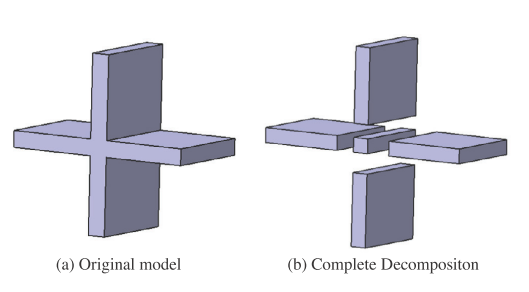
\includegraphics[width=0.6\linewidth]{images/zhudecomp}
		\caption{Convex Partitioning (Source: Zhu~\cite{Zhu2016})}
		\label{fig:introduction:zhudecomp}
	\end{figure} 

%%\bigskip

Figure~\ref{fig:introduction:zhudecomp} shows convex partitioning of the input solid shape, mentioned as ``Original model'' into convex sub-solids, shown under ``Complete Decomposition''. 
Decomposition has been used effectively for defeaturing. Some of the salient approaches are mentioned below.

Sang Hun Lee~\cite{Lee2005, SangHunLee2005, Lee2009} elaborated a method to reorder features in the history tree and then to re-execute the history of the reordered features up to the given level of details (LoD). Since the model re-evaluation is computationally intensive, he used cellular topology (CT) created by decomposition, for increasing the performance. One of the major limitations of this approach is that once the model is converted to CT, its feature update capability would cease to exist, making it difficult for any further modifications.

%Yoonhwan Woo~\cite{Woo2009} proposed a method to recognize subtractive features on Brep model, thus eliminating the problem of looking at the history tree. This approach lacked coverage in terms of variety of features being recognized and thus, was limited to simple shapes.

Byung Chul Kim~\cite{Kim2014} generated  feature based model by Cellular or Wrap or Split or Feature decomposition and then suppressed by type and size. This method can be applied widely but was limited in the recognition capabilities.

Decomposition, like feature-recognition, is highly heuristic and error prone, especially for complex models. Thus, defeaturing using decomposition, has limitations while using for real life complex part models.

%%Below is the summary of the relevant decomposition-based Defeaturing approaches:
%%
%%\csvreader[longtable=|p{0.15\linewidth}|p{0.1\linewidth}|p{0.2\linewidth}|p{0.2\linewidth}|p{0.17\linewidth}|p{0.17\linewidth}|,
%%    table head=\toprule \bfseries Author & \bfseries Input& \bfseries  Method & \bfseries  Approach& \bfseries  Advantages& \bfseries  Limitations \\ \midrule \endhead,% \bottomrule \endfoot,
%%  late after last line=\\\bottomrule,
%%  before reading={\catcode`\#=12},after reading={\catcode`\#=6},    
%%    late after line=\\\hline]%
%%{litsurvey_decomp_defeature.csv}{Author=\Author, Input=\Input, Method=\Method, Approach=\Approach, Advantages=\Advantages ,Limitations=\Limitations}%
%%{\Author  & \Input&  \Method &\Approach & \Advantages & \Limitations}%

Table~\ref{tbl:survey:alldefeature} presents the summary of the above mentioned defeaturing approaches:

\todo{Review comment: Merge all tables together. [DONE]}

%%\bigskip

\csvreader[longtable=|p{0.15\linewidth}|p{0.1\linewidth}|p{0.15\linewidth}|p{0.15\linewidth}|p{0.17\linewidth}|p{0.17\linewidth}|,
    table head=\toprule \bfseries Author & \bfseries Input& \bfseries  Method & \bfseries  Approach& \bfseries  Advantages& \bfseries  Limitations \\ \midrule \endhead \caption{CAD Model Defeaturing Approaches}\label{tbl:survey:alldefeature} \endlastfoot,% \bottomrule \endfoot,
  late after last line=\\\bottomrule,
  before reading={\catcode`\#=12},after reading={\catcode`\#=6},    
    late after line=\\\hline]%
{litsurvey_all_defeature.csv}{Author=\Author, Input=\Input, Method=\Method, Approach=\Approach, Advantages=\Advantages ,Limitations=\Limitations}%
{\Author  & \Input&  \Method &\Approach & \Advantages & \Limitations}%


%%\bigskip

\subsection{Observations on CAD Model Defeaturing Approaches}\label{sec:litsurvey:obsdefeat}

\todo{Review comments: Do not directly put bullets. Give some precursor, enumerate or just write verbose summary. [ADDED FEW LINES. REMOVED CITATIONS]}

\added{Research in defeaturing approaches has been going on for decades and remains a challenging problem to solve. Varied requirements from different domains, complexities of input parts and the critical role of engineering judgment in the selection rules, has made defeaturing a challenging task. Following is the list of some of the important observations from the survey of above CAD model defeaturing approaches:}

\begin{enumerate}[noitemsep,topsep=2pt,parsep=2pt,partopsep=2pt]
	\item Most defeaturing approaches take either Brep or mesh as input CAD model. Small irrelevant features are recognized and removed. Feature recognition, being a heuristic methodology, is not successful on many complex parts. Thus, success of defeaturing is limited and non-deterministic.
	\item In case of feature based CAD models, due to ready access to features, removal of irrelevant features and subsequent regeneration of the model is easier. The challenge remains in selection of features to be removed.
	\item Size based defeaturing, where features below certain size threshold are removed, is the most prevalent approach. Apart from this, few approaches suggest use of application specific engineering judgment as well, such as, holes in the load path should not be removed however small they are, etc.
	\item Full feature dimensions are used by some of the approaches for deciding size based removal of features. Features volumes, typically are consumed partially in the model when they get added. Thus using full feature dimensions gives wrong candidates for defeaturing.
	\item Feature dependencies fetch child features which are not originally selected for removal. These dependencies should be minimized by appropriate modeling practices.
\item Identification of the irrelevant features, only by their feature types, cannot be used blindly across all domains. For example, a rib-like feature may not be relevant in the metal flow analysis, but may be relevant in the heat transfer analysis. 
\end{enumerate}

\added{It is thus, observed that CAD model defeaturing approaches largely do not leverage feature information and are not customized to the application domain.}

Following section elaborates the second important aspect of the model simplification, i.e. the dimension reduction approaches, specifically the midsurface generation methods, along with their state of the art.

\section{Midsurface Generation Approaches}

Midsurface is part of a family of geometric entities known as ``Medial'' objects. Other members of the family are Medial Axis Transform, Skeleton, Symmetric Axis, etc.~\cite{Butlin2009}. A medial object represents the input solid shape with one or two dimensions less and lies midway of it~\cite{Armstrong}.  Medial objects such as skeleton and medial surface, are 2 and 1 dimension less than the input solid shape, respectively.

%%\bigskip

	\begin{figure} [h]
		\centering
		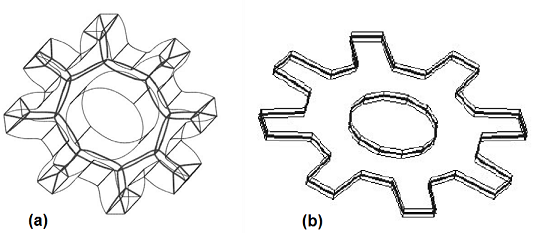
\includegraphics[width=0.7\linewidth]{images/mat2d3d}
		\caption{Skeleton and Medial Surface of Gear Shape (Source: Ramanathan~\cite{Ramanathan2004, Ramanathan2005})}
		\label{fig:litsurvey:mat2d3d}
	\end{figure}
	
%%\bigskip	

Figure~\ref{fig:litsurvey:mat2d3d}a shows a 1D representation, called ``skeleton'', of a 3D gear shaped solid. Figure~\ref{fig:litsurvey:mat2d3d}b shows a 2D representation, called ``medial surface'', of a similar 3D gear shaped solid. 

Medial objects are used for different applications, such as pattern recognition, approximation, similarity estimation, collision detection, animation, matching, CAE, etc. Processing a medial object is quicker as they are simpler, of lower dimensions and still represent the input shape by mimicking it faithfully. Some of the widely used medial object computation approaches are Medial Axis Transform (MAT)~\cite{Harry1967},  Chordal Axis Transform (CAT)~\cite{Prasad2007}, Thinning~\cite{Lam1992}, and Pairing~\cite{Rezayat1996}, etc.  

\todo{Review comment: In general instead of giving a terse reference of figure, it is better ti say Fig X.X indicates/depicts/shows schematic/diagrammatic representation of various media axis computation approaches. [DONE]}

%%\bigskip

	\begin{figure} [h]
		\centering
		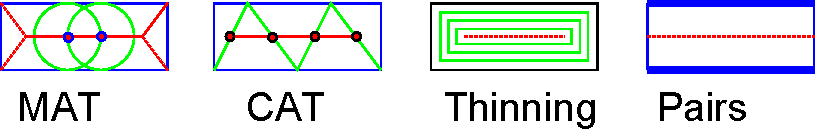
\includegraphics[width=0.7\linewidth]{images/MedialMethodsOnlyShort_1.pdf}
		\caption{Medial Generation Approaches}
		\label{fig:litsurvey:medials}
	\end{figure}
	
%%\bigskip	
 
Figure~\ref{fig:litsurvey:medials} shows their schematic representations. Lines in the middle (dotted) depict medial object of an input shape represented by outer rectangle. In MAT, medial is obtained by tracing loci of the centers of maximal disk, shown as circle, traversing within the input shape. In CAT, the input shape is triangulated first, then medial is obtained by joining midpoints of the sides of the triangle. In Thinning, medial is obtained by successively offsetting the boundary of the input shape, till no further offset is possible. In Pairing, opposite geometric entities are found and their pairs are formed. Medial is computed as an entity equidistant from the paired entities.

Approaches shown in Figure~\ref{fig:litsurvey:medials} can be classified into two categories, viz. formal and heuristics. In formal approaches, a medial object is computed mathematically, in a formal manner, whereas in heuristic approaches, the medial object is computed based on empirical, rules-based procedure.
Out of the approaches shown in Figure~\ref{fig:litsurvey:medials}, MAT, CAT and Thinning are considered as formal approaches, whereas Pairing is classified as a heuristic approach.  Following sub-sections elaborate these approaches and towards end of each category, comparison table is presented along with the summary of observations.

The formal approaches are:

\begin{enumerate}[noitemsep,topsep=2pt,parsep=2pt,partopsep=2pt]
	\item  Medial Axis Transform (MAT).
	\item Chordal  Axis Transform (CAT).
	\item Thinning and Straight Skeleton.
	\item Parametric Equations.
\end{enumerate}

The heuristic approaches are:

\begin{enumerate}[noitemsep,topsep=2pt,parsep=2pt,partopsep=2pt]
	\item Face pairing or Midsurface abstraction.
	\item Feature-based midsurface.
	\item Decomposition based midsurface.
\end{enumerate}

Following section elaborates theses approaches in details.
 
\subsection{Generating Midsurface by Medial Axis Transform (MAT)}

MAT is a locus of the center of an inscribed disc of maximal diameter as it rolls around the object interior. Figure~\ref{fig:litsurvey:mat} depicts representation of MAT in 2D (called Medial Axis Curve). MAT algorithms, typically, utilize Voronoi diagrams and Delaunay triangulation. 


%%\bigskip

\begin{figure}[!h]
\centering
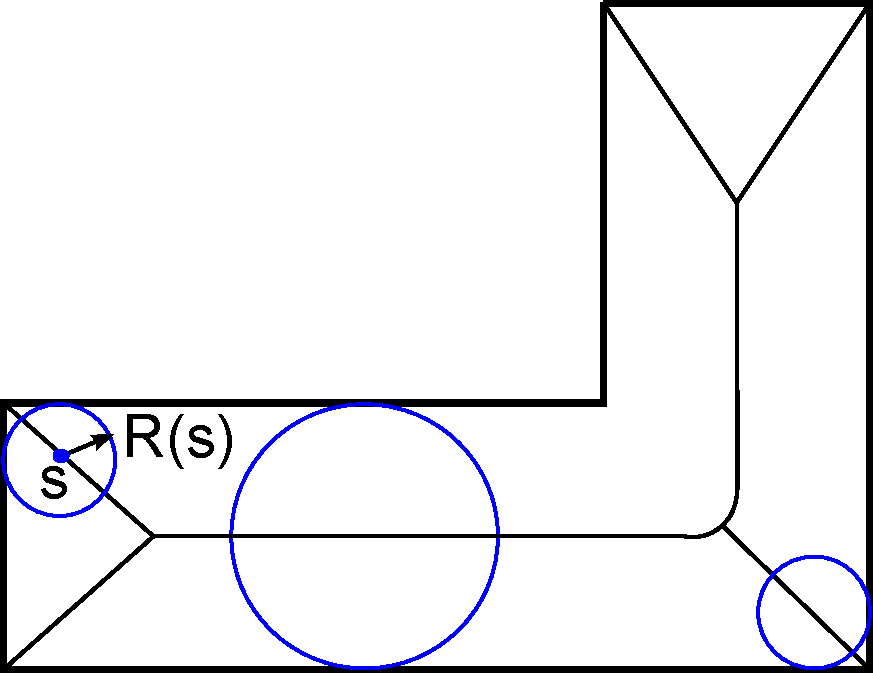
\includegraphics[width=0.3\linewidth]{images/MAT1.pdf}
\caption{Medial Axis Transform (Source: Sheen~\cite{Sheen2008})}
\label{fig:litsurvey:mat}
\end{figure}


%%\bigskip

MAT was first introduced by Blum~\cite{Harry1967} in 1967. He proposed Medial Axis Transform (MAT) as a representation that embodies the skeleton of an object as well as the width of the object at every point on the skeleton.  

Robinson~\cite{Robinson2006, Robinson2007}, Stanley~\cite{Stanley2010} used the MAT approach, either to detect thin portions or to compute midcurve. \deleted{All these approaches needed post processing to remove undesired branches. More in-depth survey of approaches is presented by Attali~\cite{Attali2004}. }

In one of the recent approaches, Automex~\cite{Automex} used Scale Axis Transform, a modified MAT method, where rolling balls are scaled to address the issue of branches and perturbations. Although the approach is promising, it suffers limitations in complex cases where it creates unnecessary topological fragments.

Ramanathan~\cite{Ramanathan2004} pointed out that the MAT falls short in its ability to reflect the local topology of the part exactly. This is because of the extraneous portions and non-linear entities that occur due to convex and concave corners in the domain. 
%\added{Figure~\ref{fig:litsurvey:midcurve}a shows branches at corners $A,B,C,D$}. On the other hand, Figure~\ref{fig:litsurvey:midcurve}b shows mid-curve that resembles the original geometry to a greater extent. 
He modified the MAT method to remove undesired branches. \added{Figure~\ref{fig:litsurvey:midcurve}a depicts the usual MAT output showing branches such as $A-E1,B-E1,F1-C,F1-D$, whereas Figure~\ref{fig:litsurvey:midcurve}b shows midcurve output where spurious branches have been replaced by two extension forming a continuous line, thus mimicking the original shape.}

	\begin{figure} [h]
		\centering
		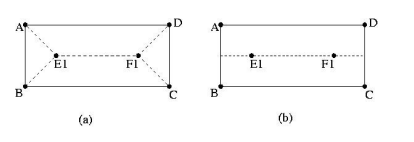
\includegraphics[width=0.7\linewidth]{images/midcurve}
		\caption{Modified MAT for Midcurve Computation (Source: Ramanathan~\cite{Ramanathan2004} )}
		\label{fig:litsurvey:midcurve}
	\end{figure}
	
Many post-processing methods have been proposed to remove branches undesired compared to midsurface expected (Fig.~\ref{fig:litsurvey:medials})~\cite{Attali2004,  Tam2003, Algazi1992,Brandt1992, Ogniewicz1995, Tam2002, Turkiyyah1995,Turkiyyah1997, KaoJune1999}, but they are not practically useful.

\todo{Review comment: Serial refs can be stacked. [DONE]}


\todo{Review comment: Merge all th tables related to MAT, CAT Thinning etc. [DONE. COMBINED OBSERVATIONS AS WELL]}

%%Below is the summary of the relevant MAT approaches:
%%
%%\csvreader[longtable=|p{0.17\linewidth}|p{0.09\linewidth}|p{0.12\linewidth}|p{0.2\linewidth}|p{0.17\linewidth}|p{0.17\linewidth}|,
%%    table head=\toprule \bfseries Author & \bfseries Input& \bfseries  Medial& \bfseries  Approach& \bfseries  Advantages& \bfseries  Limitations \\ \midrule \endhead,% \bottomrule \endfoot,
%%  late after last line=\\\bottomrule,
%%  before reading={\catcode`\#=12},after reading={\catcode`\#=6},    
%%    late after line=\\\hline]%
%%{litsurvey_mat.csv}{Author=\Author, Input=\Input, Method=\Method, Approach=\Approach, Advantages=\Advantages ,Limitations=\Limitations}%
%%{\Author  & \Input&  \Method &\Approach & \Advantages & \Limitations}%


%%\subsubsection{Observations on MAT}
%%\begin{itemize}[noitemsep,topsep=2pt,parsep=2pt,partopsep=2pt]
%%	\item Biggest strength of MAT is that it can be computed of any shape, thick or thin. Being formally defined reversal, meaning , ``given a MAT compute the original shape'', is possible.
%%	\item Major drawback of this method is that it creates unnecessary branches and its shape is smaller than the original corresponding faces.
%%	\item  MAT based approaches also suffer from robustness problem. A slight change in base geometry forces re-computation of MAT and the results could very well be different than the original.
%%	\item Although MAT approaches have been around for decades and are fairly mature, its usage in midcurve-midsurface generation is still very complex and difficult to ensure appropriate topology.
%%
%%\end{itemize}


\subsection{Generating Midsurface by Chordal  Axis Transform (CAT)}	

\todo{Review comment: What is CAT based approach. [ADDED LINES]}

For computing CAT, in case of a 2D shape, the input is meshed by Constrained Delaunay Triangulation (CDT). Midpoints of the chords i.e. sides of the triangles, are joined to form the medial~\cite{QuadrosRoshanOwenBrewerShimada2004}. In case of 3D solid shape as an input, a tetrahedral (tet) mesh is generated without inserting interior nodes and then midsurface is generated by fitting through midpoints of tetrahedral elements' faces, called chordal faces. Figure~\ref{fig:litsurvey:cat} shows CAT approach applied to both, 2D and 3D input shapes. Figure~\ref{fig_cat2d} shows how 2D input  shape is meshed with triangles and then a curve is fitted through the midpoints of the triangle edges (chords). Figure~\ref{fig_cat3d} shows result of tetrahedral elements meshing and computation of CAT by fitting a surface through midpoints of the tetrahedral elements faces (chordal faces).

%%\bigskip

	\begin{figure}[!h]
	\centering     %%% not \center
	\subfloat[CAT Curve for 2D Input]{\label{fig_cat2d}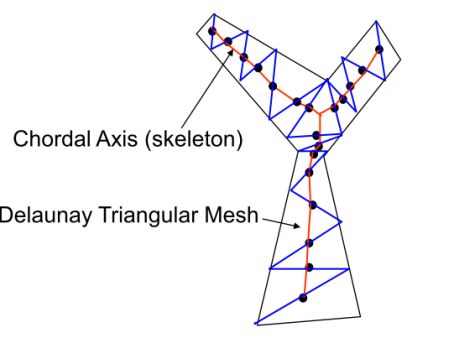
\includegraphics[width=0.4\linewidth]{images/CAT}} \quad
	\subfloat[CAT Surface for 3D Input]{\label{fig_cat3d}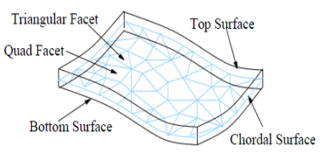
\includegraphics[width=0.4\linewidth]{images/CAT3D}}
	\caption{Chordal  Axis Transform (Source: Quadros~\cite{QuadrosRoshanOwenBrewerShimada2004} )} %%%%%%%% ADD (\{citeYogeshIITG2014}) LATER
	\label{fig:litsurvey:cat}
	\end{figure}
	
%%\bigskip

CAT was first proposed by Prasad~\cite{Prasad2007} and developed extensively by Quadros~\cite{QuadrosShimadaOwen2004, QuadrosRoshanOwenBrewerShimada2004, Quadros2008}.
Quadros~\cite{QuadrosShimadaOwen2004, Quadros2008, Quadros2000} triangulated the input shape with single layered constrained meshing, classified cells based on positions and had each unit compute their own midsurface patches, which later were joined. With this approach, medials of large, complex parts can be calculated, but the limitation is that getting the uniform, one layered triangulation itself is challenging. Thus, this method is not used for practical CAE analysis.
	
	
%%Below is the summary of the relevant CAT approaches:
%%
%%\csvreader[longtable=|p{0.17\linewidth}|p{0.09\linewidth}|p{0.12\linewidth}|p{0.2\linewidth}|p{0.17\linewidth}|p{0.17\linewidth}|,
%%    table head=\toprule \bfseries Author & \bfseries Input& \bfseries  Medial& \bfseries  Approach& \bfseries  Advantages& \bfseries  Limitations \\ \midrule \endhead,% \bottomrule \endfoot,
%%  late after last line=\\\bottomrule,
%%  before reading={\catcode`\#=12},after reading={\catcode`\#=6},    
%%    late after line=\\\hline]%
%%{litsurvey_cat.csv}{Author=\Author, Input=\Input, Method=\Method, Approach=\Approach, Advantages=\Advantages ,Limitations=\Limitations}%
%%{\Author  & \Input&  \Method &\Approach & \Advantages & \Limitations}%
%%
%%\subsubsection{Observations on CAT}
%%
%%\begin{itemize}[noitemsep,topsep=2pt,parsep=2pt,partopsep=2pt]
%%	\item  Similar to MAT, the biggest advantages of CAT is that it can be computed for any thick or thin shape.
%%	\item The major limitation of CAT approach is that mesh has to be generated before the Chordal axis surface can be created. Creating constrained, single layer meshes on complicated solid CAD models are at times difficult.
%%\end{itemize}

\subsection{Generating Midsurface by Thinning Approaches}

\replaced{Thinning approaches}{The algorithms in this category} simulate a grass-fire like process~\cite{Harry1967}. In the grass-fire process, when boundary of grass field is set to fire, the fire front successively shrinks the field inwards till it reaches the intersections. \added{In the context of medial computation, the grass-fire process is simulated by making object thinner and thinner in successive iterations} by offsetting its boundary toward its interior until it vanishes. %The amount of offset at each step depends on topology and connectivity of the original objects~\cite{KaoJune1999}.

By iteratively offsetting the boundary curves and efficiently identifying the breakpoints, Montanari~\cite{Montanari1969} could locate all the critical points on the medial axis, together with the geometry of the skeleton segments that connect them. Gursoy~\cite{Gursoy1989} extended his work by including circular arcs as boundary elements.

Aichholzer~\cite{Aichholzer1991, Aichholzer2006} was one of the first proponents of a special thinning method called ``Straight Skeletons''. 

%%\bigskip

	\begin{figure} [!h]
		\centering
		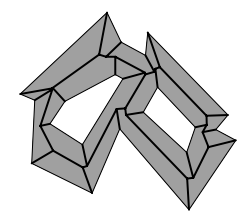
\includegraphics[width=0.4\linewidth]{images/Straight}
		\caption{Straight Skeletons (Source: Aichholzer~\cite{Aichholzer1991} )}
		\label{fig:litsurvey:straight}
	\end{figure}
	
%%\bigskip

Figure \ref{fig:litsurvey:straight} shows an example of Straight Skeleton of a 2D shape. At each vertex, angle bisectors are produced, which are used to partition the interiors. The lines joining intersection pins of the bisector forms the medial curve. Although this method can take both, thick and thin shapes, it is restricted to only polygons. Another limitation is that, similar to MAT, it also produces unwanted branches which need to be removed.

%%Below is the summary of the relevant Thinning approaches:
%%
%%\csvreader[longtable=|p{0.17\linewidth}|p{0.1\linewidth}|p{0.12\linewidth}|p{0.2\linewidth}|p{0.17\linewidth}|p{0.17\linewidth}|,
%%    table head=\toprule \bfseries Author & \bfseries Input& \bfseries  Medial& \bfseries  Approach& \bfseries  Advantages& \bfseries  Limitations \\ \midrule \endhead,% \bottomrule \endfoot,
%%  late after last line=\\\bottomrule,
%%  before reading={\catcode`\#=12},after reading={\catcode`\#=6},    
%%    late after line=\\\hline]%
%%{litsurvey_midsurfthinning.csv}{Author=\Author, Input=\Input, Method=\Method, Approach=\Approach, Advantages=\Advantages ,Limitations=\Limitations}%
%%{\Author  & \Input&  \Method &\Approach & \Advantages & \Limitations}%
%%
%%
%%\subsubsection{Observations on Thinning Approaches}
%%\begin{itemize}[noitemsep,topsep=2pt,parsep=2pt,partopsep=2pt]
%%	\item Thinning approaches are based on split events of the straight line skeleton gives counter-intuitive results if the polygon contains sharp reflex vertices.
%%	\item It generates unwanted branches which need to be removed to arrive at the required midcurve.
%%\end{itemize}

%-------------------------------------------------------------------------------------
\subsection{Generating Midsurface by Parametric Equations Approach}	
\replaced{Parametric}{This} approach takes two parent curves and fits a curve through equidistant points from both the curves~\cite{Elber1999, Fischer1997}. Figure~\ref{fig:litsurvey:parametric} shows two input curves $C_1(u)$ and $C_2(v(u))$ generating midpoint $O(u.v(u0))$. Loci of the $O$s is the midcurve. \added{The same approach is extended to surfaces as well.}

%%\bigskip

	\begin{figure} [!h]
		\centering
		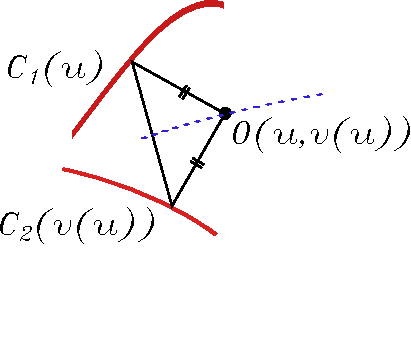
\includegraphics[width=0.4\linewidth]{images/MidcurvesDefn}
		\caption{Parametric Midcurve (Source: Fischer~\cite{Fischer1997} )}
		\label{fig:litsurvey:parametric}
	\end{figure}
	
%%\bigskip

In Fischer's~\cite{Fischer1997} parametric approach, sketch profile of features like Extrude, Revolve is extracted. The piecewise linear midpoints  of intersecting pair of matched normals are generated. They are then fitted with the Bspline midcurve. Midcurve is extruded or revolved to generate the midsurface.  This approach gives fairly good results in generating midsurface patches per feature, however, does not elaborate on joining connections between the midsurface patches.

In one of the most recent approaches reported by Zhu et. al~\cite{Zhu2015, Zhu2016}, the input surfaces are triangulated, then for each point pair a middle point is computed, which are then fitted with a surface, resulting into a midsurface. While this method removes need for post-processing self-intersecting surfaces, it has major drawbacks that it needs surface pairs to be readily available to begin with and requires expensive triangulation.

%%Below is the summary of the relevant Parametric Equations  approaches:
%%
%%\csvreader[longtable=|p{0.17\linewidth}|p{0.1\linewidth}|p{0.12\linewidth}|p{0.2\linewidth}|p{0.17\linewidth}|p{0.17\linewidth}|,
%%    table head=\toprule \bfseries Author & \bfseries Input& \bfseries  Medial& \bfseries  Approach& \bfseries  Advantages& \bfseries  Limitations \\ \midrule \endhead,% \bottomrule \endfoot,
%%  late after last line=\\\bottomrule,
%%  before reading={\catcode`\#=12},after reading={\catcode`\#=6},    
%%    late after line=\\\hline]%
%%{litsurvey_midsurfparam.csv}{Author=\Author, Input=\Input, Method=\Method, Approach=\Approach, Advantages=\Advantages ,Limitations=\Limitations}%
%%{\Author  & \Input&  \Method &\Approach & \Advantages & \Limitations}%
%%
%%\subsubsection{Observations on Parametric Approaches}
%%\begin{itemize}[noitemsep,topsep=2pt,parsep=2pt,partopsep=2pt]
%%	\item The two input curves/surfaces may not be in one-to-one form. In such cases maintaining continuity would a be challenge.
%%	\item Quality of surface generated by these method depends on the sampling done to compute the midpoints.
%%\end{itemize}

Table~\ref{tbl:survey:matcatparamthin} outlines the summary of relevant formal approaches.

%%\bigskip

\csvreader[longtable=|p{0.15\linewidth}|p{0.1\linewidth}|p{0.15\linewidth}|p{0.15\linewidth}|p{0.17\linewidth}|p{0.17\linewidth}|,
    table head={\toprule \bfseries Author & \bfseries Input& \bfseries  Medial& \bfseries  Approach& \bfseries  Advantages& \bfseries  Limitations \\ \midrule \endhead \caption{Formal Midsurface Generation Approaches}\label{tbl:survey:matcatparamthin} \endlastfoot},% \bottomrule \endfoot,
  late after last line=\\\bottomrule,
  before reading={\catcode`\#=12},after reading={\catcode`\#=6},    
    late after line=\\\hline]%
{litsurvey_matcatthinparam.csv}{Author=\Author, Input=\Input, Method=\Method, Approach=\Approach, Advantages=\Advantages ,Limitations=\Limitations}%
{\Author  & \Input&  \Method &\Approach & \Advantages & \Limitations}%


%%\bigskip


\subsection{Observations on Formal Midsurface Generation Approaches}\label{sec:survey:observationsformal}

\todo{[MAKING A NEW (TO BE CONFIRMED) CLASSIFICATION O METHODS INTO FORMAL AND HEURISTIC.Calling MAT, CAT, Thinning and Parametric as Formal methods as they are mathematical and definitive in output. Calling remaining methods like Face Pairing, Feature based, decomposition based as Heuristic as they are non-formal, non-mathematical. Need to discuss and confirm]}


Approaches based on MAT, CAT, Thinning and Parametrization have been in research for decades. All of them, being formal-mathematical, can be applied to a wide variety of shapes, and not restricting themselves to only thin-walled shapes. Following are some of the salient observations with regards to these approaches:

\todo{Review comment: Add one liner as differentiator between previous and following approaches. [DONE]}

\begin{itemize}[noitemsep,topsep=2pt,parsep=2pt,partopsep=2pt]
	\item Biggest strength of the formal approaches like MAT is that it can be computed for any shape, thick or thin. Being formally defined, the converse or reversal process (meaning ``given a MAT, compute the original shape'') is possible.
	\item Major drawback of MAT, Thinning methods is that it creates unnecessary branches and its shape is smaller than the original corresponding faces.
	\item  MAT based approaches also suffer from robustness problem. A slight change in base geometry forces re-computation of MAT and the results could very well be different from the original.
	\item Although MAT approaches have been around for decades and are fairly mature, its usage in midcurve-midsurface generation is still very complex and difficult to ensure appropriate topology.
	\item The major limitation of CAT approach is that mesh has to be generated before. Creating constrained, single layer meshes on complicated CAD models are, at times, difficult.
	\item Thinning approaches are based on split events of the straight line skeleton giving counter-intuitive results if the polygon contains sharp reflex vertices.
	\item In Parametric approach, the two input curves or surfaces may not be in one-to-one form. In such cases maintaining continuity can be challenging.
	\item Quality of surface generated by parametric approach depends on the sampling done to compute the midpoints.
\end{itemize}

\added{Thus formal approaches to compute midcurve or midsurface have some major limitations, rendering them less useful for the practical scenarios. Following approaches are more heuristic in nature and they are found to have wider applicability in the practical scenarios.} 

\subsection{Generating Midsurface by Face Pairing Approach}
%\subsection{Generating Midsurface by Face Pairing or Midsurface Abstraction Approach}

Midsurface Abstraction (MA) or Face-pairing method was first proposed by Rezayat~\cite{Rezayat1996}. In this approach, face pairs are identified on the thin-wall part's Brep model. It involves casting a ray from a face in the Brep's material direction, to find the opposite face. Such opposite faces form face-pairs. Each face pair generates its own midsurface patch. Connectivity information between respective face-pairs is used to decide which midsurface patches join each other. The midsurface patches are joined, either by trimming or extending them to come to a common location.

%%\bigskip

	\begin{figure} [!h]
		\centering
		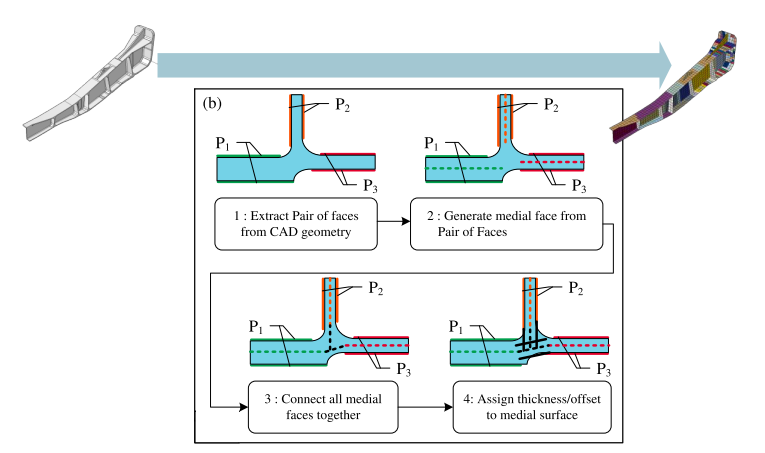
\includegraphics[width=\linewidth]{images/manual}
		\caption{Generating Midsurface by Face Pairing (Source: Boussuge~\cite{Boussuge2014})}
		\label{fig:litsurvey:manual}
	\end{figure}
	
%%\bigskip

Figure~\ref{fig:litsurvey:manual} depicts the face pairing approach. Figure~\ref{fig:litsurvey:manual}:1  shows face pairs being detected. In Figure~\ref{fig:litsurvey:manual}:2, midsurface patches are generated for each face pair. In Figure~\ref{fig:litsurvey:manual}:3, patches are extended or trimmed to join at common locations. In Figure~\ref{fig:litsurvey:manual}:4, thickness values are assigned on the midsurface.


\todo{[Removed both the paragraphs and merged info in the first paragraph]}
	
Rezayat claims that the face-pairing approach has benefits over the MAT approach because the resultant geometry is cleaner and requires less post-processing. However the face pairing approach suffers from severe difficulties especially in complex models, such as identifying correct face pairs and joining midsurface patches properly.
	
%Flow of algorithm is as below:
%\begin{itemize}[noitemsep,topsep=2pt,parsep=2pt,partopsep=2pt]
%	\item In the surface pairing step, all the faces excepting the end-caps and of thick region are paired. It involves ray casting from (any) seed face in material direction to find opposite-pair face.
%	\item connectivity between respective faces of pairs is preserved by tagging.
%	\item The paired faces are then interpolated to create mid-surface patches, which may be intersecting. 
%	\item The topological adjacency information (tagged info) is used to trim the patches
%\end{itemize}

%Thus, MA~\cite{Rezayat1996, Fischer1997} involves constructing the 3D mid-surface for a part model by connecting/sewing the mid-surface patches obtained from 'pairs of surfaces'. This requires a 'pairing strategy' that thus far requires human intervention. Connecting various mid-surface patches require 3D Boolean operations. This surface-pairing approach has benefits over MAT approaches because the resultant geometry is cleaner and requires less reconstruction. However the surface pairing approach also has problems because it can be difficult to identify all of the surface pairs.

%%Ramanathan~\cite{Ramanathan2004} states that though the mid-surface has desirable properties as an abstraction of 3D shape, a formal definition of the midsurface is not available. This makes it difficult to develop algorithms for generating the mid-surface of an object. Also, unlike MAT, the mid-surface is not unique for a given object and this adds to the difficulties in realizing the mid-surface. There have been very few efforts reported for the construction of mid-surface.

%The mid-surface abstraction is applied to the entire model simultaneously and no error threshold is defined to select the parts of the model to which abstraction is to be applied. In this approach, small features such as holes are simplified automatically when the mid-surface is generated. Material distribution is effectively represented in this approach by introducing thickening in the direction of the draft and by introducing thinning in the direction of the undercut.

%%Chong et al., who presented an approach to break the Brep model into parts and then applied mid-surface abstraction for simplification for finite element model preparation application\cite{Chong2004}.

S H Lee and D P Sheen~\cite{Sheen2008} proposed Solid Deflection method leveraging face-pair detection and face geometry replacement. Topology was kept intact while bigger of the two faces was offset-ed. Tolerance was increased so as to make them look like connected but they were not. Their work appears to be very limited in the range of input shapes it would handle.
%
%	\begin{figure} [!h]
%		\centering
%		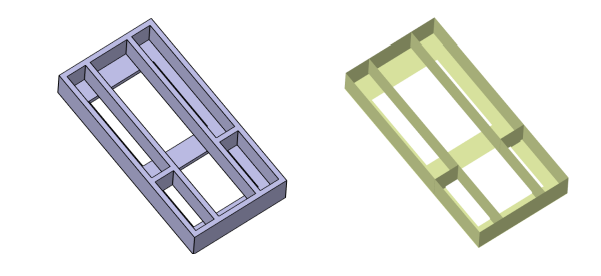
\includegraphics[width=0.6\linewidth]{images/SheenMidsurf}
%		\caption{Midsurface Abstraction (Source: Sheen~\cite{Sheen2008} )}
%		\label{fig:litsurvey:sheen}
%	\end{figure}

\todo{Removed the figure. One is good enough}

Sungchan Kim et al.~\cite{Kim2005} developed various approaches for model simplification, mainly focusing on defeaturing aspects, but they also mentioned usage of face-pairing for dimension reduction in case of thin solids. Their approach was simplistic and lacked details on joining of midsurface patches.

%%Below is the summary of the relevant Face Pairing approaches:
%%
%%
%%\csvreader[longtable=|p{0.17\linewidth}|p{0.11\linewidth}|p{0.15\linewidth}|p{0.2\linewidth}|p{0.17\linewidth}|p{0.17\linewidth}|,
%%    table head=\toprule \bfseries Author & \bfseries Input& \bfseries  Method& \bfseries  Approach& \bfseries  Advantages& \bfseries  Limitations \\ \midrule \endhead,% \bottomrule \endfoot,
%%  late after last line=\\\bottomrule,
%%  before reading={\catcode`\#=12},after reading={\catcode`\#=6},    
%%    late after line=\\\hline]%
%%{litsurvey_midsurfpairing.csv}{Author=\Author, Input=\Input, Method=\Method, Approach=\Approach, Advantages=\Advantages ,Limitations=\Limitations}%
%%{\Author  & \Input&  \Method &\Approach & \Advantages & \Limitations}%

Face-pairing algorithms are implemented in the commercial CAD-CAE applications. They have automatic as well as manual input. Thus, despite the limitations, these applications are able to generate mid-surfaces for a range of realistic models. Approaches seen so far were based on Brep model. Following section elaborates midsurface generation approaches using feature information.

%A medial surface toolkit is available from TranscenData~\cite{Transcendata2009},
%and the surface-pairing algorithm is implemented in UGS I-DEAS-NX~\cite{SDRC2009}.
%%\subsubsection{Observations on Midsurface-abstraction Approaches}
%%
%%\begin{itemize}[noitemsep,topsep=2pt,parsep=2pt,partopsep=2pt]
%%\item Very popular method amongst commercial implementation as it provides the user the ability to pick appropriate face pairs in case the automatic detection fails. It does not create branches.
%%\item Automatic Face pair detection is error prone in non-trivial situations. Also, connections between patches are missed in complex shapes.
%%\item  Major drawback is that it may not be able to compute midsurface for very complicate parts.
%%\end{itemize}


\subsection{Generating Midsurface by Feature-based Approaches}

In feature based CAD, a model is built step-by-step using features. At each step,  input parameters of the features are used to build tool-bodies. These tool bodies are then boolean-ed with the model built till that step. 

%%\bigskip

	\begin{figure} [!h]
		\centering
		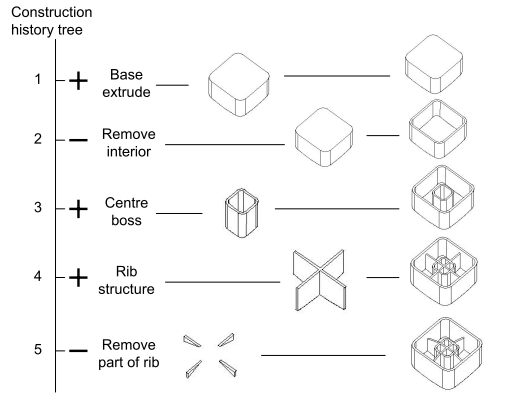
\includegraphics[width=0.75\linewidth]{images/stolttree}
		\caption{Construction of CAD Model by Features (Source: Stolt~\cite{Stolt2006} )}
		\label{fig:litsurvey:stolttree}
	\end{figure}

%%\bigskip

Figure~\ref{fig:litsurvey:stolttree} shows Stolt's~\cite{Stolt2006} depiction of construction history, i.e. feature tree of a CAD model. The shapes shown in the middle are the tool bodies, which are boolean-ed (shown as $+$ and $-$) to build the model. In many cases, the tool-bodies are of relatively simple shapes \added{such as extruded or revolved sections,} thus making feature based algorithms simpler and deterministic. There have been a few attempts to use the feature information in the computation of the midsurface. Use of features has not been done extensively in the past because feature specific information was not exposed by the CAD systems, either through file format or through Application Programming Interfaces (APIs). These days, however, most of the widely used CAD modelers provide APIs to expose feature information, giving rise to their usage in CAD algorithms. 

%%%%\bigskip
%%
%%	\begin{figure} [!h]
%%		\centering
%%		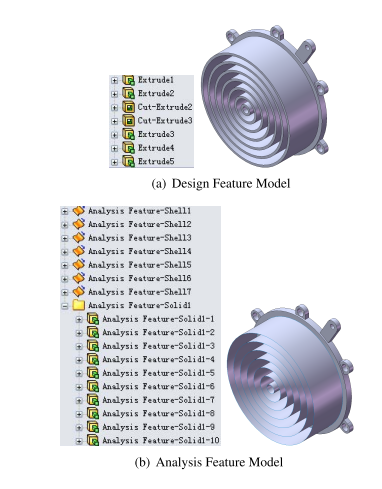
\includegraphics[width=0.6\linewidth]{images/CaoMidsurf}
%%		\caption{Midsurface of a Feature based CAD model (Source: Cao~\cite{Cao2009} )}
%%		\label{fig:litsurvey:cao}
%%	\end{figure}
%%
%%%%\bigskip

Stolt~\cite{Stolt2005} worked on features such as ``Pad'', ``Pocket'', extracted sketches and analyzed if there are parallel curves to form mid-segments. These segments were used for extrusion with same parameters as the original feature.

%%\bigskip

	\begin{figure} [!h]
		\centering
		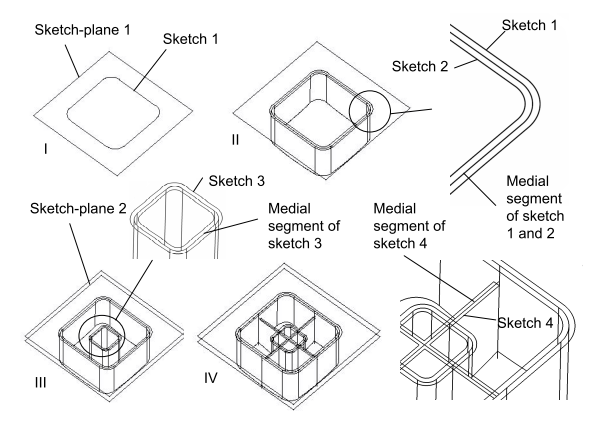
\includegraphics[width=0.75\linewidth]{images/stoltmids}
		\caption{Construction of Feature-based Midsurface (Source: Stolt~\cite{Stolt2006} )}
		\label{fig:litsurvey:stoltmids}
	\end{figure}

%%\bigskip

Figure~\ref{fig:litsurvey:stoltmids} shows the process of building feature based midsurface proposed by Stolt ~\cite{Stolt2006}. Figure~\ref{fig:litsurvey:stoltmids}:I shows the first feature's sketch. Figure~\ref{fig:litsurvey:stoltmids}:II shows the first feature, along with its midsurface computed from the medial segment of the first sketch. Similarly Figure~\ref{fig:litsurvey:stoltmids}III and IV show, features being added along with their midsurface.

Robinson et al.~\cite{Robinson2007} while working on mixed-dimensional model for aerospace structures utilized information in CAD feature tree to locate sketches and then features built on top of it like Sweep, Revolve. The work appears to be limited due to processing of a small set of singular features only and no consideration seems to be given to joining process.

These approaches are comparatively less in number and restrict themselves to midsurface patches creation. They do not leverage feature information effectively in setting up appropriate connections between patches.

%%As Brep is still the most widely used format, some apparhches do Feature recognition to extract features and then apply their midurface generation aleotithms.
%% 
%%Figure~\ref{fig:litsurvey:cao} shows how Cao~\cite{Cao2009}~\cite{Cao2011} decomposed the final Brep and recognized additive remnant swept primitives for which midsurface patches were computed either by sweeping corresponding midcurve or offsetting one of the faces or by interpolating the faces. But there no details mentioned about joining logic for the patches.
%%
%%Boussuge et al. ~\cite{Boussuge2013,Boussuge2013a} split the Brep into protrusion features and then idealized each to midsurface. The joining logic presented in this work was very restricted to 3 interaction types and also the features recognized were only positive protrusions.

\todo{[REMOVED FIGURE FROM HERE AND LET IT BE WHERE IT IS MOST APPROPRIATE]}


%%Below is the summary of the relevant feature based midsurface approaches:
%%
%%\csvreader[longtable=|p{0.17\linewidth}|p{0.11\linewidth}|p{0.15\linewidth}|p{0.2\linewidth}|p{0.17\linewidth}|p{0.17\linewidth}|,
%%    table head=\toprule \bfseries Author & \bfseries Input& \bfseries  Medial& \bfseries  Approach& \bfseries  Advantages& \bfseries  Limitations \\ \midrule \endhead,% \bottomrule \endfoot,
%%  late after last line=\\\bottomrule,
%%  before reading={\catcode`\#=12},after reading={\catcode`\#=6},    
%%    late after line=\\\hline]%
%%{litsurvey_midsurffbd.csv}{Author=\Author, Input=\Input, Method=\Method, Approach=\Approach, Advantages=\Advantages ,Limitations=\Limitations}%
%%{\Author  & \Input&  \Method &\Approach & \Advantages & \Limitations}%
%%
%%
%%\subsubsection{Observations on Feature based Midsurface Approaches}
%%
%%\begin{itemize}[noitemsep,topsep=2pt,parsep=2pt,partopsep=2pt]
%%\item Feature based approaches bring definitiveness in model simplification which in turn helps midsurface idealization
%%\item Feature information has not been extensively used for variety of reasons such as access-restrictions on the proprietary feature information, unsuitable non-manifold structure, as well as the impracticality to include CAE structures in CAD software.
%%\item Most of the approaches restrict themselves to midsurface patches creation and do not leverage feature boolean information in setting up appropriate connections between patches.
%%\end{itemize}


\subsection{Generating Midsurface by Decomposition Based Approaches}

Decomposition is a process of partitioning given shape into non overlapping sub-shapes. It can be applied on both, 2D and 3D CAD shapes. Decomposed sub-shapes compute the medial object. If 2D sketch profiles is the input then, midcurves are computed and if 3D Brep solid is the input then midsurface is computed. 


%%\bigskip

	\begin{figure} [!h]
		\centering
		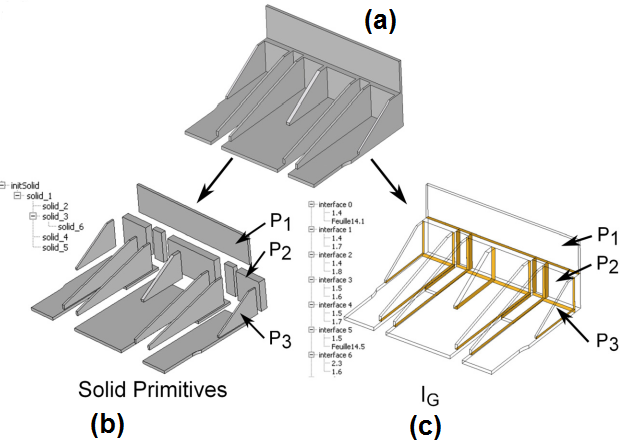
\includegraphics[width=0.75\linewidth]{images/boussugedecomp}
		\caption{Generating Midsurface by Decomposition (Source: Boussuge~\cite{Boussuge2013a} )}
		\label{fig:litsurvey:boussugedecomp}
	\end{figure}

%%\bigskip

Figure~\ref{fig:litsurvey:boussugedecomp} depicts Boussuge's~\cite{Boussuge2013a} approach of midsurface by decomposition.
Figure~\ref{fig:litsurvey:boussugedecomp}a shows the input Brep solid CAD model. Figure~\ref{fig:litsurvey:boussugedecomp}b shows its decomposition into sub-shapes, called ``solid primitives''. Figure~\ref{fig:litsurvey:boussugedecomp}c shows midsurface computed for each solid primitive.
\todo{[MOVED PARAGRAPHS OF POLYGON DECOMPOSITION AND MIDCURVE CREATION TO THAT CHAPTER. MIDCURVE COULD HAVE BEEN RETAINED HERE, BUT THEN WITHOUT POLY DECOMP IT WAS NOT MAKING SENSE.]}

%\subsubsection{Generating Midcurve by 2D Decomposition}

%%Midcurve by 2D decomposition methods are based on Divide-and-Rule policy. The 2D profile is subdivided into simpler sub-shapes for which medial can be computed readily. Midcurves of all such sub-shapes are merged to get the final well-connected midcurve.
%%
%%Keil~\cite{Keil94} presented an approach based on Convex partitioning. It finds all possible ways to remove reflexivity of these vertices and then takes the one that requires fewest diagonals. Lien et. al.~\cite{Lien2004} decomposed polygons 'approximately' based on iterative removal of the most significant non-convex feature. 
%%
%%Bayazit~\cite{Bayazit} presented a polygon decomposition method based on Concave (Reflex) angle partitioning. Although the output was far better than if usual meshing had been employed, the drawback was it left out some corner cases giving more than necessary divisions.
%%
%%Below is the summary of the relevant profile decomposition approaches:
%%
%%\csvreader[longtable=|p{0.17\linewidth}|p{0.11\linewidth}|p{0.15\linewidth}|p{0.2\linewidth}|p{0.17\linewidth}|p{0.17\linewidth}|,
%%    table head=\toprule \bfseries Author & \bfseries Input& \bfseries  Method & \bfseries  Approach& \bfseries  Advantages& \bfseries  Limitations \\ \midrule \endhead,% \bottomrule \endfoot,
%%  late after last line=\\\bottomrule,
%%  before reading={\catcode`\#=12},after reading={\catcode`\#=6},    
%%    late after line=\\\hline]%
%%{litsurvey_polydecomp.csv}{Author=\Author, Input=\Input, Method=\Method, Approach=\Approach, Advantages=\Advantages ,Limitations=\Limitations}%
%%{\Author  & \Input&  \Method &\Approach & \Advantages & \Limitations}%
%%
%% Choi~\cite{Choi1997} subdivided the planar region with holes into smaller simply connected planar sub regions that overlap only at the joints where subdivision occurs. Approximated medials based on Bezier-Bernstein curves are computed for individual sub-regions. Decomposition of planar shapes  into regular (non-intersecting) and singular (intersecting regions) and its application to skeletonization has been widely researched~\cite{Rocha99} as well.
%% 
%% Rocha~\cite{Rocha98}~\cite{Rocha99} presented skeletonization approach for images which primarily worked on vertices. Sub-shapes computed mid-segments which were joined at the connections. Although this approach could address many shapes, it lacked comprehensive coverage and did not do very well for simple joints like T and L
%%
%%Bag~\cite{Bag2011} computed mid-segments for character image which preserve the local characteristics.
%% 
%% Below is the summary of the relevant midcurve computation approaches:
%% 
%%\csvreader[longtable=|p{0.17\linewidth}|p{0.11\linewidth}|p{0.2\linewidth}|p{0.2\linewidth}|p{0.17\linewidth}|p{0.17\linewidth}|,
%%    table head=\toprule \bfseries Author & \bfseries Input& \bfseries  Medial& \bfseries  Approach& \bfseries  Advantages& \bfseries  Limitations \\ \midrule \endhead,% \bottomrule \endfoot,
%%  late after last line=\\\bottomrule,
%%  before reading={\catcode`\#=12},after reading={\catcode`\#=6},    
%%    late after line=\\\hline]%
%%{litsurvey_midcurvedecomp2d.csv}{Author=\Author, Input=\Input, Method=\Method, Approach=\Approach, Advantages=\Advantages ,Limitations=\Limitations}%
%%{\Author  & \Input&  \Method &\Approach & \Advantages & \Limitations}%
%%
%%\subsubsection{Observations on Midcurve by 2D Decomposition Approaches}
%%
%%\begin{itemize}[noitemsep,topsep=2pt,parsep=2pt,partopsep=2pt]
%%	\item Polygon decomposition rules depend on the application context, accuracy, characteristics  and aspect ratio of the sub-polygons. In CAE, meshing is one of the widely used decomposition methods. Approiach used in this work aims at minimum partitioning to result into primitive shaped sub-polygons.
%%	\item Midcurve generation depends on the quality of the sub-polygons generated in the decomposition. Non-primitive, skewed shapes result in ill-midcurves.
%%\end{itemize}


%\subsubsection{Generating Midsurface by Cellular Decomposition}

\added{The sub-shapes generated by decomposition are called as ``Cells''. Cells not only simplify the geometries to work with but also introduce possibility of parallelization. With these advantages, researchers have used decomposition extensively in CAD (as voxels), CAM (machining pockets), CAE (meshing), etc.}

%%The present research leverages decomposition for devising generic midsurface computations algorithm. One of the primary reasons for gaps in the midsurface results is due to ill-recording  of feature interaction in the input shape. Thus, same interaction could not get replicated on the midsurface patches.  To address issues related to feature interactions, this research leverages feature based CAD model represented as a set of decomposed cells. 

\todo{[MOVED CELLULAR DECOMPOSITION SPECIFIC SURVEY TO THAT CHAPTER. KEEPING APPROACHES HAVING MIDSURFACE ONLY]}

%%Following subsections present state-of-the-art in Cellular Decomposition, solid model based decomposition, feature based cellular topology and midsurface based on cellular decomposition.
%%
%%\todo{Including few of the cellular decomposition methods that have not been used for midsurface, because, even those methods are useful reference in the decomposition we leveraged}
%%
%%Woo~\cite{Woo2003} found that in typical Cell Decomposition each of the faces having a concave edge is extended such that it interests the whole model, creating cells. As this would generate a large number of unnecessary cells, concept of `maximal volume' came (Figure~\ref{fig:litsurvey:maxcd}), which collects some of the cells, based on certain criteria, to be merged together, thus reducing the number with a few modifications. 
%% 
%%\begin{figure}[!h]
%%\centering     %%% not \center
%%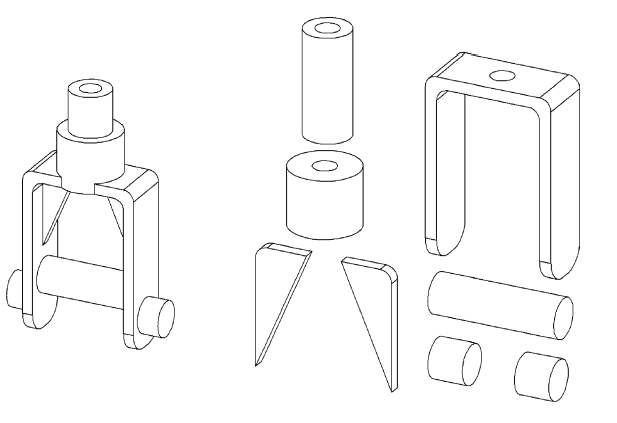
\includegraphics[width=0.5\linewidth,valign=t]{images/maximalvolume}
%%\caption{Maximal Cellular Decomposition (Source : Woo~\cite{Woo2003})}
%%\label{fig:litsurvey:maxcd}
%%\end{figure}
%% 
%%Bih-Yaw Shih~\cite{Shih1996} presented an automated swept volume detection and decomposition algorithm. This approach was computationally intensives for complex model. 
%%
%%Yong Lu~\cite{LuGadhTautges2001} reported the work on shape recognition and volume decomposition to automatically decompose a CAD model into hex meshable volumes. 
%%
%%Yoonhwan Woo~\cite{Woo2002}~\cite{Woo2003}~\cite{Woo2003a}~\cite{Woo2006}~\cite{Woo2009}  did extensive work in fast and maximal cellular decomposition. His method was superior to other prevalent method but was restricted to analytical surface shapes.
%%
%%%Quite a few attempts to compute the midsurface using cellular decomposition are found in the literature~\cite{Chong2004, Cao2009,Cao2011,Woo2013}.
%%
%% Below is the summary of the relevant Cellular Decomposition approaches:
%% 
%%\csvreader[longtable=|p{0.17\linewidth}|p{0.11\linewidth}|p{0.2\linewidth}|p{0.2\linewidth}|p{0.17\linewidth}|p{0.17\linewidth}|,
%%    table head=\toprule \bfseries Author & \bfseries Input& \bfseries  Method & \bfseries  Approach& \bfseries  Advantages& \bfseries  Limitations \\ \midrule \endhead,% \bottomrule \endfoot,
%%  late after last line=\\\bottomrule,
%%  before reading={\catcode`\#=12},after reading={\catcode`\#=6},    
%%    late after line=\\\hline]%
%%{litsurvey_celldecomp.csv}{Author=\Author, Input=\Input, Method=\Method, Approach=\Approach, Advantages=\Advantages ,Limitations=\Limitations}%
%%{\Author  & \Input&  \Method &\Approach & \Advantages & \Limitations}%

%%Cellular decomposition, in the context of the current research, is the division of a feature based CAD model into non-volumetrically overlapping, but surface-overlapping sub-solids (called ``cells'').  Research in  cellular decomposition, especially for Computer-aided Manufacturing (CAM) and CAE has been going on for decades. Feature based cellular decomposition, which deals with either decomposition of features, or feature-recognition after decomposition,  has also been  researched extensively~\cite{Bidarra1993, BidarraKrakerBronsvoort1998, Woo2003, JaeLee2004, Treeck, Boussuge2013a, Wu2014, Woo2014}. There have been a few attempts to compute a midsurface using cellular-decomposition as well~\cite{Chong2004, Woo2013, Boussuge2013, Zhu2015}
%% 
%%\csvreader[longtable=|p{0.17\linewidth}|p{0.11\linewidth}|p{0.2\linewidth}|p{0.2\linewidth}|p{0.17\linewidth}|p{0.17\linewidth}|,
%%    table head=\toprule \bfseries Author & \bfseries Input& \bfseries  Method & \bfseries  Approach& \bfseries  Advantages& \bfseries  Limitations \\ \midrule \endhead,% \bottomrule \endfoot,
%%  late after last line=\\\bottomrule,
%%  before reading={\catcode`\#=12},after reading={\catcode`\#=6},    
%%    late after line=\\\hline]%
%%{litsurvey_featurecells.csv}{Author=\Author, Input=\Input, Method=\Method, Approach=\Approach, Advantages=\Advantages ,Limitations=\Limitations}%
%%{\Author  & \Input&  \Method &\Approach & \Advantages & \Limitations}%

%\subsubsection{Generating Midsurface by Feature based Cellular Decomposition Approaches}

%Feature based Cellular data model has been research and its usage in various downstream applications has been studied. Kernels like ACIS provide cellular topology which can be enhanced to have owner feature information.  
Quite a few attempts to compute the midsurface using cellular decomposition are found in the literature~\cite{Chong2004, Cao2009,Cao2011,Woo2013}. 

%%\bigskip

%
%\begin{figure}[!h]
%\centering     %%% not \center
%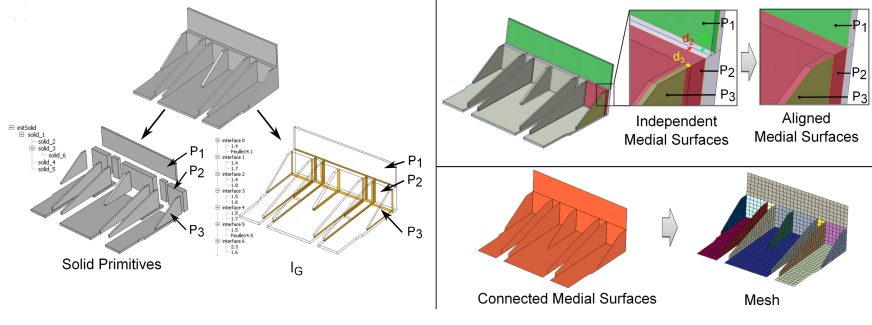
\includegraphics[width=0.85\linewidth,valign=t]{images/boussugemidsurf}
%\caption{Decomposition, Protrusions, Midsurfaces (Source : Boussuge~\cite{Boussuge2013a})}
%\label{fig:litsurvey:boussuge}
%\end{figure}


\begin{figure}[!h]
\centering     %%% not \center
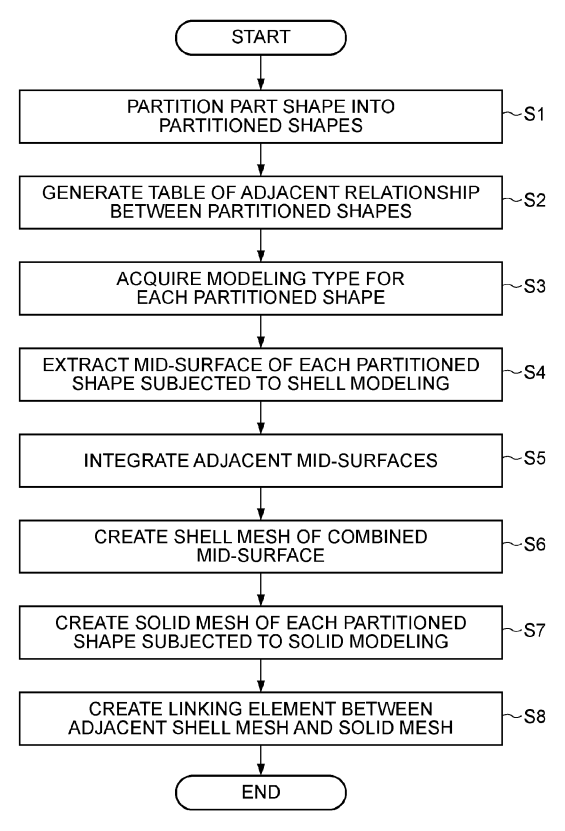
\includegraphics[width=0.45\linewidth,valign=t]{images/Kageura}
\caption{Generating Midsurface by Partition Approach (Source : Kageura~\cite{Kageura2009})}
\label{fig:litsurvey:Kageura}
\end{figure}

%%\bigskip

Chong et al.~\cite{Chong2004} split the Brep model into sub-volumes which, in turn, extracted their own midsurface patches.

Kageura~\cite{Kageura2009} filed US Patent 2009/0271156A1 in which, as shown in Figure~\ref{fig:litsurvey:Kageura}, an input shape is partitioned first, adjacency information is generated, midsurface patches are extracted and combined.

Cao~\cite{Cao2009, Cao2011} decomposed the final Brep model and recognized additive remnant swept primitives, got their sketches, computed midcurves for edge-pairs and created midsurface patches but the joining logic was not much elaborated. 

Boussuge et al. ~\cite{Boussuge2013,Boussuge2013a}  split the Brep model at concave edges, recognized (only) positive  protrusion features in the sub-volumes and then idealized each to a midsurface with a joining logic restricted to only a couple of hard-coded interaction types. Figure~\ref{fig:litsurvey:boussugedecomp} shows how a model is split into solid primitives, midsurface patches are generated and they are joined at the interfaces $I_G$s.

Woo~\cite{Woo2013} used his maximal volume technique \cite{Woo2006, Woo2009} and computed midsurface for each sub-volume using face-pair technique. It worked only for analytical surfaces and parallel face pairs

%% Below is the summary of the relevant Feature based Cellular Decomposition Approaches:
%% 
%%\csvreader[longtable=|p{0.17\linewidth}|p{0.11\linewidth}|p{0.2\linewidth}|p{0.2\linewidth}|p{0.17\linewidth}|p{0.19\linewidth}|,
%%    table head=\toprule \bfseries Author & \bfseries Input& \bfseries  Medial& \bfseries  Approach& \bfseries  Advantages& \bfseries  Limitations \\ \midrule \endhead,% \bottomrule \endfoot,
%%  late after last line=\\\bottomrule,
%%  before reading={\catcode`\#=12},after reading={\catcode`\#=6},    
%%    late after line=\\\hline]%
%%{litsurvey_midsurfdecomp3d.csv}{Author=\Author, Input=\Input, Method=\Method, Approach=\Approach, Advantages=\Advantages ,Limitations=\Limitations}%
%%{\Author  & \Input&  \Method &\Approach & \Advantages & \Limitations}%

 Table~\ref{tbl:survey:midsheuristic} presents a summary of relevant heuristic midsurface generation approaches:
 
 
%%\bigskip

\csvreader[longtable=|p{0.15\linewidth}|p{0.1\linewidth}|p{0.15\linewidth}|p{0.15\linewidth}|p{0.17\linewidth}|p{0.17\linewidth}|,
%    table head=\toprule \bfseries Author & \bfseries Input& \bfseries  Medial& \bfseries  Approach& \bfseries  Advantages& \bfseries  Limitations \\ \midrule \endhead,% \bottomrule \endfoot,
    table head={\toprule \bfseries Author & \bfseries Input& \bfseries  Medial& \bfseries  Approach& \bfseries  Advantages& \bfseries  Limitations \\ \midrule \endhead \caption{Heuristic Midsurface Generation Approaches}\label{tbl:survey:midsheuristic} \endlastfoot},% \bottomrule \endfoot,
     late after last line=\\\bottomrule,
  before reading={\catcode`\#=12},after reading={\catcode`\#=6},    
    late after line=\\\hline]%
{litsurvey_heuristics.csv}{Author=\Author, Input=\Input, Method=\Method, Approach=\Approach, Advantages=\Advantages ,Limitations=\Limitations}%
{\Author  & \Input&  \Method &\Approach & \Advantages & \Limitations}%


%%\bigskip

\subsection{Observations on Heuristic Midsurface Generation Approaches}

Extensive research has been done on the heuristic methods for computing midsurface, such as midsurface abstraction (face pairing), feature based, cellular decomposition based, etc. These are more widely used in commercial applications, compared to the formal approaches such as MAT, CAT, etc. In-spite of a huge demand, the heuristic methods have limited usage, especially in case of complex models. Following are the salient observations on heuristic methods:

\begin{itemize}[noitemsep,topsep=2pt,parsep=2pt,partopsep=2pt]
\item Face pairing is widely used approach amongst the commercial CAD-CAE applications, as it provides the user the ability to pick appropriate face pairs in case the automatic detection fails. 
\item Automatic Face pair detection is error prone for complex CAD models as input. Joining midsurface patches also does not work robustly for them. Due to these problems, Face pairing suffers from limitations such as extensive use of hard-coded rules for detecting edge or face pairs, support for limited types of geometries, limited range of connections, etc.
\item Midsurface by cellular decomposition approach is not used widely. Cellular decomposition can result in large number of cells, needing quite a few boolean operations, making it ineffective and unstable. Choosing correct splitting logic, maximal volume rules should help make the process optimized and robust.
\item Feature based midsurface computation approaches bring definitiveness in computation of midsurface, due to lesser use of heuristics.
\item Feature information has not been extensively used for computation of midsurface due to its inaccessibility so far. 
\item Most current feature based midsurface computation approaches restrict themselves to midsurface patches creation and do not leverage feature boolean information in setting up appropriate connections between patches.
 \end{itemize}

Overall, both formal and heuristic approaches present strengths and limitations in different aspects of computing midsurface. Out of them, use of defeaturing, leveraging feature information and decomposition appear promising in computation of a quality midsurface. 

The quality of midsurface is validated by various techniques, primarily to detect failures such as gaps, overlaps, etc.
%The present research work attempts to address these limitations by leveraging feature-based, decomposition approaches along with use of new concepts such as generalization, feature based decomposition, etc.
Following section elaborates state of the art for techniques used in validating the quality of the output midsurface.

\deleted{So, this research does not need to utilize the maximal (\cite{Woo2002}) volume strategies that have to be employed due to a large number of cells computed during the global intersections. This research expects that the FBCD should generate the part  decomposed in such a way that each cell represents a correctly assigned owning-feature.More details about methods for computing medial objects can be found in the survey paper by Kulkarni et. al~\cite{Yogesh2010}.}
 
\section{Validation Approaches for Generated Midsurfaces} \label{sec:litsurvey:validation}

Even after huge demand, extensive research and wide availability in the commercial CAD-CAE applications, quality of the midsurface computed is still a concern. Validating the output midsurface is therefore a critical step in assessing the quality, after which corrective actions can be taken.

Midsurface is expected to express the contiguous flow of the input solid's shape~\cite{Rezayat1996}. So, to be truly effective, the output midsurface needs to mimic the input thin-walled solid model, in both, geometrical and topological sense. Geometrically, the shape of the midsurface should be such that it lies in the middle (at half the thickness) of the thin-walled solid model. Topologically, the connectivity between the midsurface patches should be similar to that of their corresponding face pairs in the input thin-walled solid model. 

\deleted{It is tedious to manually inspect and validate it, especially for the complex models. The present system performs such a validation in an automated way and uses Hausdorff's distance measure to verify geometric correctness. However, as a necessary and sufficient validation, the system also carries out topological validation to verify the connectivity as well as missing surfaces or gaps.}

Thus, there are primarily two approaches to validate the output midsurfaces, namely ``geometric'' and ``topological'' ~\cite{Lockett2008} as explained below:

\begin{itemize}[noitemsep,topsep=2pt,parsep=2pt,partopsep=2pt]
\item \textbf{Geometric Validation of Midsurface}: Validates if the output midsurface lies midway of the input solid model. Lockett~\cite{Lockett2008} proposed geometric similarity index based on Hausdorff distance which provides a measure of the maximum dissimilarity between the midsurface and its associated input solid model.
\item \textbf{Topological Validation of Midsurface}:
\deleted{Use of topology for assessing the quality of midsurface is not widespread and t}
Validates if the output midsurface has similar topological connectivity as present in the input solid model. Lockett~\cite{Lockett2008} predicted topological entities of midsurface based on the topological entities of the input solid model and then used topological variants for checking the validity of the midsurface. \deleted{For geometric validation, they used the Hausdorff distance between a midsurface and its corresponding principal faces (pairs).} The main limitation of their approach is the use of geometric criteria, such as closest distance proximity or angle between faces, in the topological validations, which is contrary to the concept of topology.
\end{itemize}

\deleted{Apart from CAE, skeletal structures such as midsurface are used in CAD model comparison solutions such as shape-based retrieval, similarity assessment and difference identification ~\cite{Antoine2014}. Skeletal graph matching is one of the prominent techniques~\cite{Iyer2005} for similarity assessment. A topologically valid midsurface represents sub-shape connectivities better and thus acts as more effective shape-signature in the model comparison.}

\todo{[DROPPED THE TABLE AND OBSERVATIONS]}

%%
%% Below is the summary of the relevant Topological Invariants and Similarity assessment Approaches:
%% 
%%\csvreader[longtable=|p{0.15\linewidth}|p{0.15\linewidth}|p{0.2\linewidth}|p{0.2\linewidth}|p{0.17\linewidth}|p{0.19\linewidth}|,
%%    		table head=\toprule \bfseries Author & \bfseries Input& \bfseries  Method & \bfseries  Approach& \bfseries  Advantages& \bfseries  Limitations \\ \midrule \endhead,
%%    		late after last line=\\\bottomrule,
%%    		before reading={\catcode`\#=12},after reading={\catcode`\#=6},
%%    		late after line=\\\hline]%
%%    		{litsurvey_validation.csv}
%%    		{Author=\Author, Input=\Input, Method=\Method, Approach=\Approach, Advantages=\Advantages ,Limitations=\Limitations}%
%%    		{\Author  & \Input&  \Method &\Approach & \Advantages & \Limitations}%

%%\subsection{Observations on Midsurface Validation Approaches}
%%
%%\begin{itemize}[noitemsep,topsep=2pt,parsep=2pt,partopsep=2pt]
%%\item Apart from CAE, skeletal structures such as midsurface are used in CAD model comparison solutions such as shape-based retrieval, similarity assessment and difference identification ~\cite{Antoine2014}. 
%%\item Skeletal graph matching is one of the prominent approaches~\cite{Iyer2005} for similarity assessment. 
%%\item A topologically valid midsurface represents sub-shape connectivities better and thus acts as more effective shape-signature in the model comparison.
%%
%%
%%\end{itemize}

Although geometric approaches of validating the output midsurface are widely used, they are tedious to execute. Topological approaches are not very common and are not yet fully developed to be used practically. 

\section{Midsurface Generation Capabilities of Commercial CAD-CAE Systems}\label{sec:litsurvey:commercial}

Commercial CAD-CAE systems are in use for decades. Both systems got developed separately and are like islands of automation. The corresponding commercial systems have to transfer model data amongst themselves only through neutral file formats. Thats the reason, most of the CAD-CAE approaches are based on Brep model populated by neutral file formats, such as STEP and IGES.  Data interoperability through neutral formats is susceptible to data loss. Thus most of the data coming to preprocessing from CAD systems, has to be cleaned and healed first. But, now a days, with better CAD-CAE systems integrations, native data and in some cases even feature information is made available to CAE systems. With richer information, some of the CAD-CAE systems have improved preprocessing functionalities like defeaturing and midsurface generation. 

CAD kernels like ACIS\textsuperscript{\textregistered}, modelers like Autodesk Fusion\textsuperscript{\textregistered} and CAE packages like Altair's Hypermesh\textsuperscript{\textregistered}, Ansys\textsuperscript{\textregistered}, MSC Nastran\textsuperscript{\textregistered}, etc. do provide defeaturing capabilities mainly for CAE analysis\replaced{ that are primarily}{, but are mostly simplistic and } size-based in nature. 

Midsurface functionality is widely available in CAD-CAE systems like Autodesk Inventor\textsuperscript{\textregistered}, Parametric's Creo,  Altair's Hypermesh\textsuperscript{\textregistered}, Ansys\textsuperscript{\textregistered}, MSC Nastran\textsuperscript{\textregistered}, etc. It is observed that quality of midsurface in CAD systems is relatively lower than the CAE systems. But overall, automatic midsurface generation capabilities do not seem to be robust and meaningful for practical usages, especially for complex parts. Manual intervention and post-processing is used to correct the problems of the output midsurface.

\todo{[SHOULD I ADD SCHEMATIC DIAGRAMS SHOWING ERRORS?]}

%%\bigskip

\def \myfigcommcolumnwidth{0.85}

\begin{figure}[h!]
\centering     %%% not \center
\subfloat[Input Thin-walled Solid Model]{\label{fig_mmodel}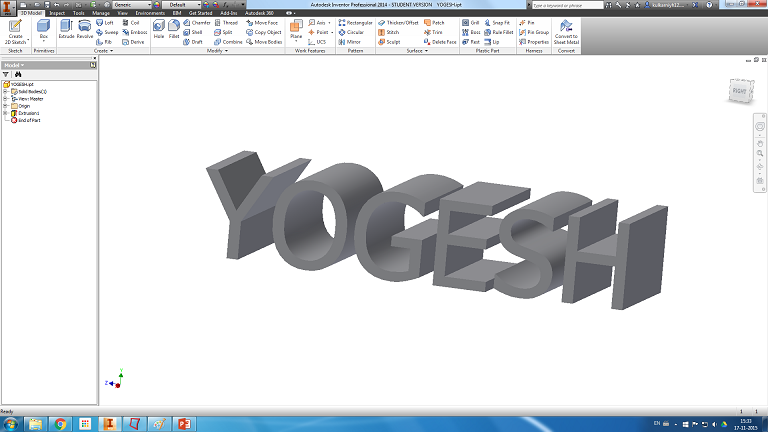
\includegraphics[width=\myfigcommcolumnwidth\linewidth]{images/Yogesh_Inv}} \quad
\subfloat[Output Midsurface of a CAD System]{\label{fig_mcad}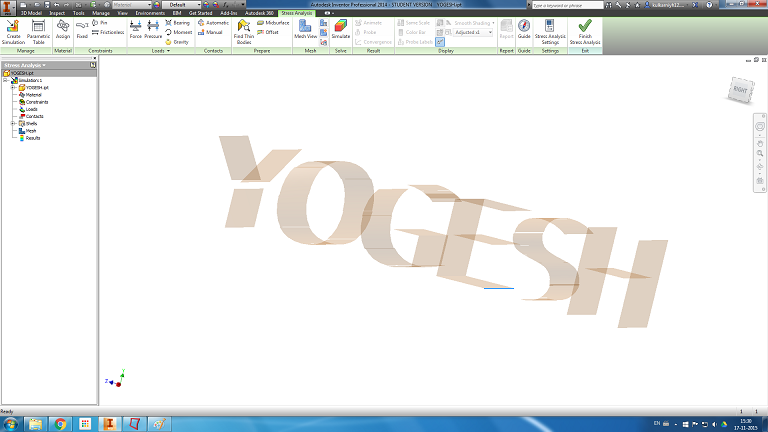
\includegraphics[width=\myfigcommcolumnwidth\linewidth]{images/Yogesh_InvMids}} \quad
\subfloat[Output Midsurface of a CAE System]{\label{fig_mcae}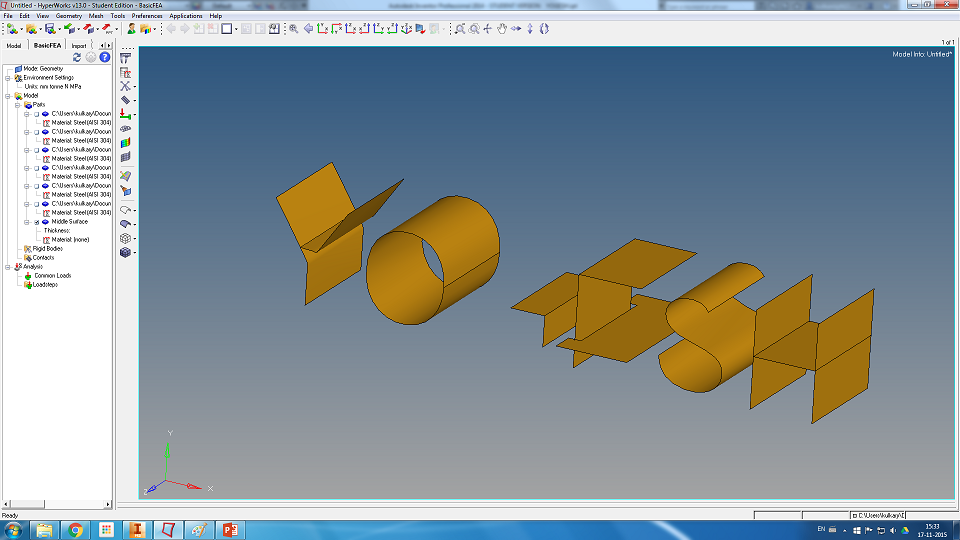
\includegraphics[width=\myfigcommcolumnwidth\linewidth]{images/Yogesh_HM_notOK}} 
\caption{Midsurfaces Generated by Commercial CAD and CAE Systems}
  \label{fig_comm}
\end{figure}


%%\bigskip

\added{Figure~\ref{fig_comm}a shows the input CAD solid model, having English alphabets shapes. These shapes are chosen for benchmarking, as it is easier to imagine their corresponding midsurfaces. The resultant midsurface is expected to look like those alphabets but in a surface form. Figure ~\ref{fig_comm}b shows midsurface output generated by a popular CAD system, whereas Figure ~\ref{fig_comm}c shows midsurface output by a widely used CAE system. Both CAD and CAE midsurface outputs show many errors, such as missing surfaces, gaps, not-lying-midway, etc.}

From the above results it is evident that there is still an ample scope for improvement in devising a robust and automated method for computing a quality midsurface.

Another detailed survey was done by conducting technical discussions with CAD-CAE experts, academicians related to various aspects of midsurface generation.  This was essentially aimed at understanding industry practices, issues etc.  Findings from theses discussions are provided in Appendix~\ref{appendix:survey}.


%\section{Observations from Survey Questionnaire}\label{sec:litsurvey:questions}

%Below is such list of understandings :
%
%\begin{itemize}[noitemsep,topsep=2pt,parsep=2pt,partopsep=2pt]
%\item 
%\end{itemize}
%
%.
%Many a times, due to complexity in recognizing forms, and due to complex interactions between them, Midsurface of the part does not follow its form and is not fully connected~\cite{Sheen2008}. Solution could be, to create Midsurface while building the model itself. 

\section{Observations from Literature Survey}\label{sec:litsurvey:summary}

%%\todo{These are the overall observations}

After analyzing various reported approaches for midsurface generation, it is observed that there has been limited success in the generation of a quality midsurface. 
\replaced{Midsurface generation approaches are computationally intensive and the errors take enormous manual interventions to correct, hence the overall process can take days or even weeks to finish.}{Practically, the complete midsurface generation cycle may take from days to weeks, depending on the complexity of the part. In spite of its demand and popularity, the existing automatic methods fail to compute a well-connected midsurface, especially for non-trivial shapes.} 
%Failures manifest in the form of gaps, missing patches, overlapping surfaces, not lying midway, not mimicking the input shape, etc. %%(Figure~\ref{fig:midsurfaceerrors}). 
%\begin{figure}[!htp]
%\centering
%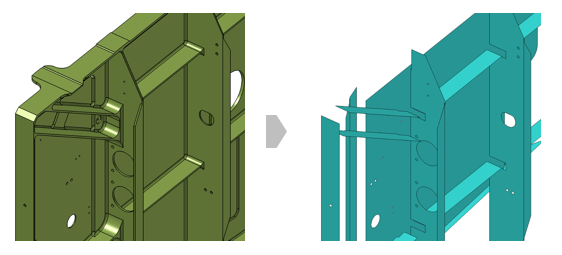
\includegraphics[width=0.7\linewidth]{images/MidsurfaceErrorsMscApex}
%\caption{Midsurface by a  latest commercial application (Source:~\cite{MScApex})}
%\label{fig:midsurfaceerrors}
%\end{figure}

Following are some of the salient observations based on the literature survey done:
 
\begin{itemize}[noitemsep,topsep=2pt,parsep=2pt,partopsep=2pt]%leftmargin=*

	\item In feature based defeaturing approaches, full feature dimensions were used for selecting features for removal thereby giving wrong results.
	\item For defeaturing, application domain-specific rules of identification of features for removal are necessary instead of identification of any feature below the `threshold' size.
	\item Past midsurface generation approaches are limited in the range of input model geometries (say, only planar or analytic surfaces), feature types (say, only extruded, positive primitives) and connection types (say, only, parallel, or perpendicular) they could handle. Due to these limitations, the output midsurface has many errors, especially for complex input solid models.
	\item  %\textbf{Midsurface Patches Generation}:  \label{sec:facepairdetection}
In face pairing approaches, finding the face-pairs in a complex part itself is very challenging. Issues like, faces may not be directly opposite to each other, may not be parallel, may have multiple opposite faces, etc. are frequent. Such wrong face pairs result in gaps in the output midsurface. %This research addresses this problem by using the Abstracted feature-information for generation of patches and avoids detection of face-pairs  (more details in section~\ref{sec:scell}). 
	\item  %\textbf{Midsurface Patches Connection}: \label{sec:facepairinteraction}
For connecting midsurface patches, there is no definitive list of connection types. Thus providing deterministic logic is not possible. This limitation results in midsurface patches not being joined properly, resulting in gaps or overlaps. %This research proposes  leveraging of feature based cellular decomposition (more details in section~\ref{sec:icell}).
\end{itemize}
 
 %The proposed approach is `generic', meaning, in principle, no such restrictions are present in this approach. It can be made to cater to any geometry types, feature types or connections. Advantages can be seen in the range of shapes handled as well as in the minimization of failures (Section~\ref{sec:results}).
 


%Based on all the surveys done and observations, following research objectives were formulated for the present research work.

\deleted{{\bfseries Thus, so far, there has been a limited success in the objective of computing a well-connected midsurface. This research plans to leverage feature information to achieve this objective.}}

\section{Research Objectives} \label{sec:introduction:rs}

The overall objective of the proposed research is to develop a system to generate a quality midsurface of sheet metal feature based CAD model \added{by developing various algorithms}. \replaced{Based on the extensive literature survey and critical analysis, following research objective are laid down, as}{This objective is broken down further into following sub-objectives}:
\begin{itemize}[noitemsep,topsep=2pt,parsep=2pt,partopsep=2pt]
\item To develop \replaced{defeaturing algorithms to simplify CAD feature model as much as possible without impacting the gross shape of the part}{ and implement a feature based model simplification (defeaturing) approach to generate a ``gross shape'', which improves midsurface generation}.
\item To develop \replaced{algorithms to represent the feature based CAD model by transforming existing set of sheet metal features to a finite set of generalized features}{and implement a feature abstraction approach to further simplify the model, by transforming each feature to a generalized form, reducing the number of scenarios to handle}.
\item To develop \replaced{algorithms for generating quality midsurfaces leveraging generalized feature based CAD model and cellular decomposition covering a wide variety of topological connectivities}{and implement a generic midsurface generation approach leveraging generalized feature form and cellular decomposition}.
\item To \replaced{come up with an approach to topologically validate the generated midsurface relative to its input CAD  model}{develop a topological validation methodology to assess correctness of the midsurface}.
\item \replaced{To implement a software system incorporating above algorithms and }{To test real-life parts to} demonstrate the efficacy of the proposed approach.
\end{itemize}

\section{Research Methodology} \label{sec:introduction:rm}
The present research work uses empirical hypothesis testing research methodology. 

%%\bigskip

	\begin{figure} [!h]
		\centering
		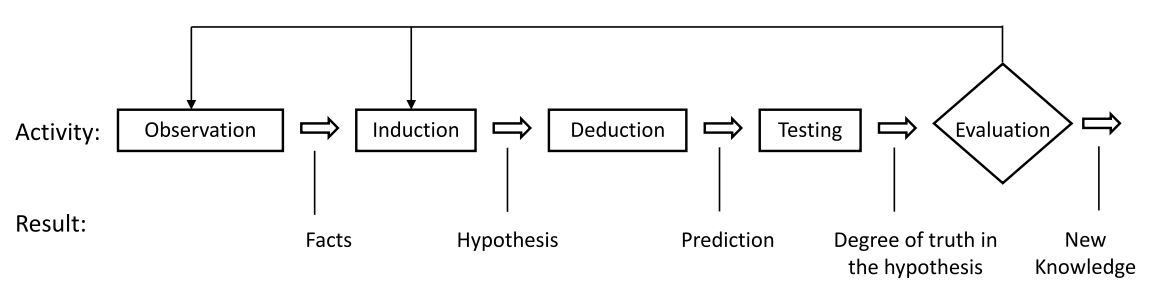
\includegraphics[width=0.9\linewidth]{images/ResearchMethodology.png}
		\caption{Empirical Hypothesis Testing Process (Source: Stolt~\cite{Stolt2008})}
		\label{fig:introduction:ResearchMethodology}
	\end{figure}

%%\bigskip
	
Figure~\ref{fig:introduction:ResearchMethodology} shows the empirical hypothesis process and its various phases. Following paragraph explains them along with their interpretation in the context of present research work. 

The empirical hypothesis testing process starts with observations, e.g. the problems observed in the current midsurface generation approaches. These facts are generalized by induction into a hypothesis, such as, the core problems in midsurface extraction are detection of sub-shapes and interactions amongst them. Predictions are then deduced from the hypothesis, such as, if the input model is simplified, generalized and decomposed, the problem could be more deterministic to handle.  A prototype is built incorporating the proposed solution. After testing the prototype, if the results are valid and acceptable, then the hypothesis is accepted as true for the time being. In the present research work, hypothesis takes the form of a set of multiple sub-hypotheses and the proposed system answers those questions. Section~\ref{sec:litsurvey:rquestions} lists the hypothesis whereas Chapter~\ref{ch:Proposal} presents the proposed system.

 \section{Research Scope}
The proposed research aims at developing algorithms for generating a quality midsurface of thin-walled \added{sheet metal} feature based CAD model. \deleted{Domain selected is of sheet metal parts.} Reason for \replaced{considering sheet metal parts in scope}{selection} is due to its wide usage in domains ranging from household items to big ships.  Better midsurface will have an enormous impact on quicker and robust product development in all these domains.

\todo{Review comment: May need concrete justification. [DONE]}

%Sheet metal models are unique in both, geometrical and topological sense. They are characterized by:
%\begin{itemize}[noitemsep,topsep=2pt,parsep=2pt,partopsep=2pt]
%\item \textbf{Constant thickness}: Made up of constant thickness blank roll.
%\item \textbf{Absences}: There are no blind holes, but only through holes, if any. 
%\item \textbf{Degeneracy}: There are no degenerate capping thickness faces (like ``Wedge'').
%\item \textbf{Cavities}: There are no embedded volumes or cavities (``bubbles'').
%\end{itemize}
%%%CAD models of sheet metal parts use a wide variety of feature such as~\cite{Liu2004} (Figure~\ref{liuFeatures}):
%%%
%%%	\begin{figure} [!h]
%%%		\centering
%%%		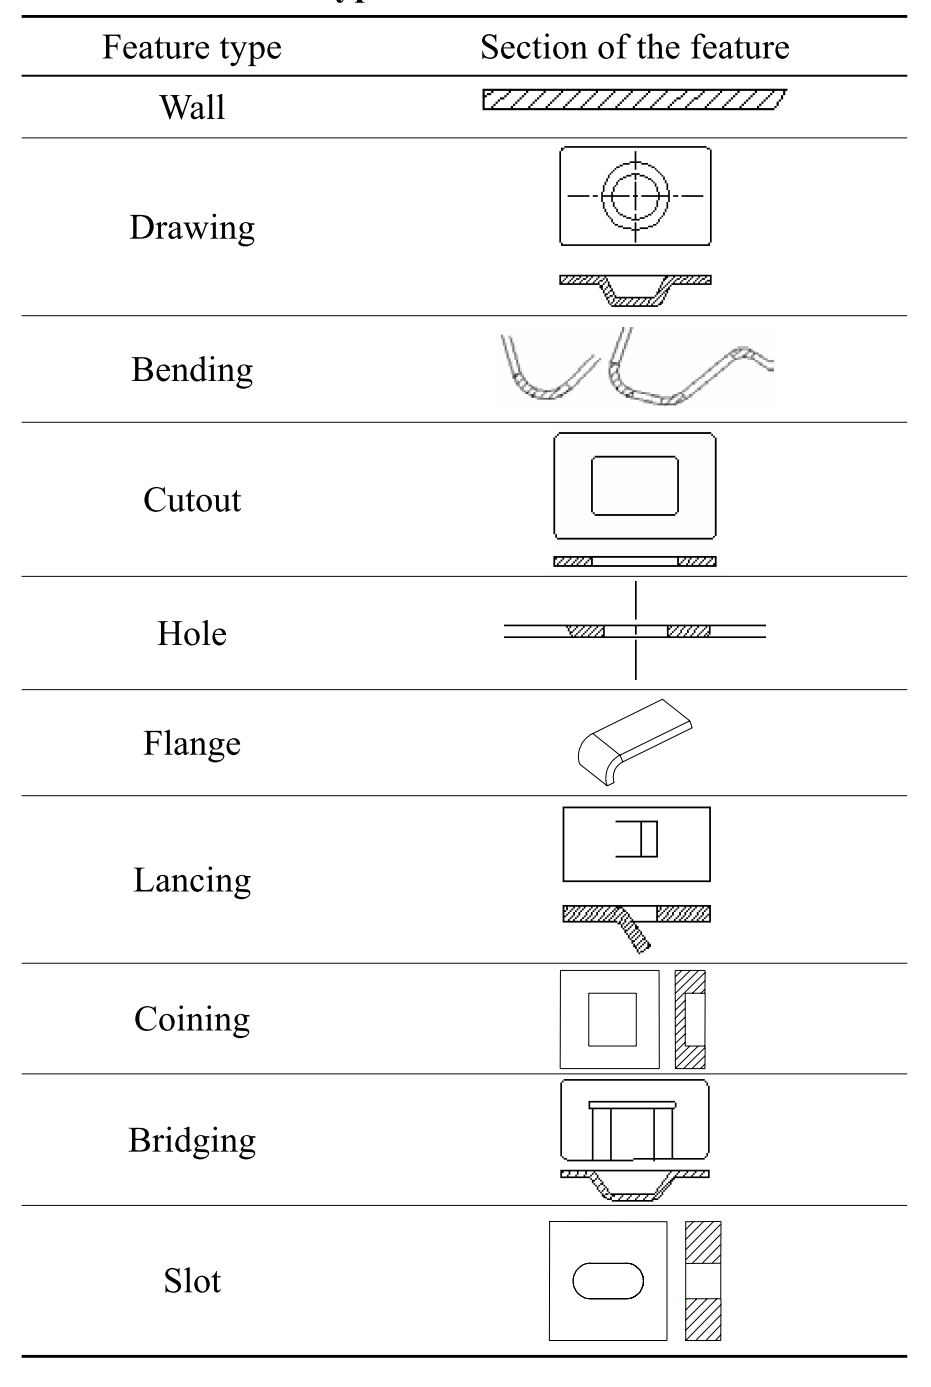
\includegraphics[width=0.6\linewidth]{images/liuFeatures}
%%%		\caption{Typical Sheet metal features~\cite{Liu2004}}
%%%		\label{fig:liufeatures}
%%%	\end{figure}
%	
%	
%\begin{minipage}[c]{0.98\linewidth}
%\begin{minipage}[t]{0.48\linewidth}
%\begin{itemize}[noitemsep,topsep=2pt,parsep=2pt,partopsep=2pt]
%\item \textbf{Primitive features}: These features an exist interdependently and form primary shape of the part, e.g. Wall, Drawing.
%\item \textbf{Add-on features}: These features must be added to the existing features and are secondary in nature, e.g. Cutout, Hole, Slot.
%\item \textbf{Connecting features}: These features act as a bridge between other features, e.g. Bend.
%\item \textbf{Composite features}: These are feature collections, .e.g. Array.
%\end{itemize}
%\end{minipage}
%\hfill
%\begin{minipage}[t]{0.48\linewidth}
%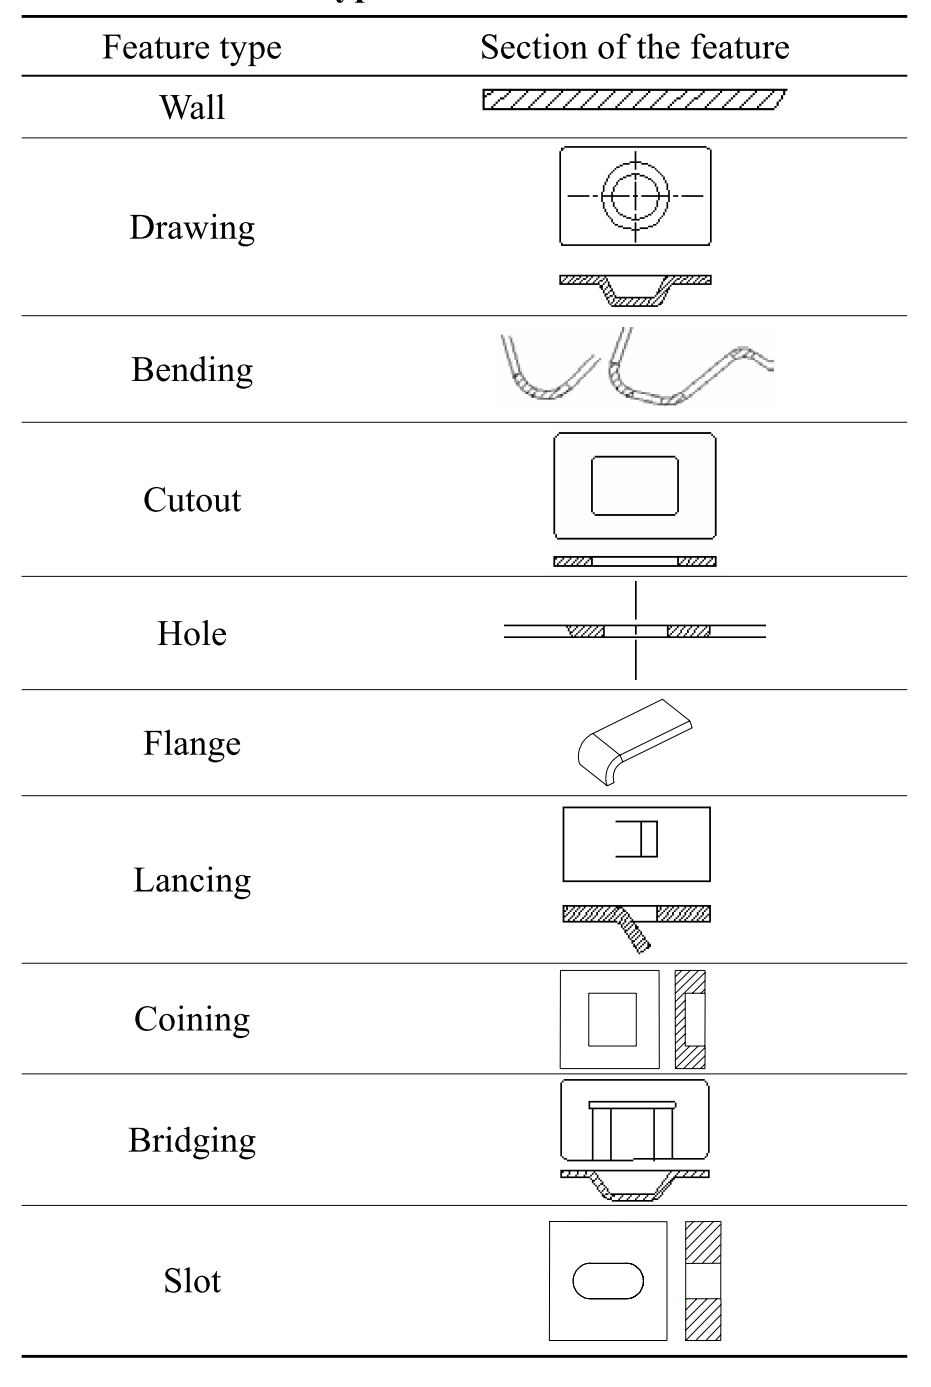
\includegraphics[width=0.52\linewidth,valign=t]{images/liuFeatures}
%\captionof{figure}{Typical Sheet metal features~\cite{Liu2004}}\label{fig:liufeatures}
%\end{minipage}
%\end{minipage}
\added{The proposed system accepts feature based CAD model built using Autodesk Inventor\textsuperscript{\textregistered}, as input. Thus, the feature based alogirthms devised in the present research, work on sheet metal features, such as, Walls, Flanges, Bends, Cutouts, etc.}
\deleted{The proposed system works on the sheet metal feature based CAD models as input, having features similar to ones mentioned above. In particular, it caters to parts made by fabrication, which show significant problems in generating midsurface, especially at the joints. It should be possible to extend it to variable-thickness components as well, with further customizations.}
\added{Autodesk Inventor\textsuperscript{\textregistered} was chosen over other CAD systems, such as Solidworks, Parametric Creo, etc. due to its free availability for students and maturity of APIs.}

Following section lists hypotheses tested by the present research work.

\section{Research Hypotheses} \label{sec:litsurvey:rquestions}

%Based on the study so far, the present research proposes a new paradigm, called ``F-SAD'' ({\bf F}eature-based, {\bf S}implification, {\bf A}bstraction, {\bf D}ecomposition), leverages use of features, simplification, abstraction and decomposition as a general approach to be used in the development of CAD functionalities. 
This research proposes following hypotheses and assesses them against the proposed system.% So, hypotheses that are going to be tested  are:

\begin{myhyp}
\label{hyp:features}
Instead of working on a Brep CAD model as input, the feature based CAD model enables computation of a well-connected midsurface.
\end{myhyp}

\begin{myhyp}
\label{hyp:Simplification}
Instead of working on a detailed CAD model, the defeatured model results in a better midsurface.
\end{myhyp}

\begin{myhyp}
\label{hyp:Abstraction}
Instead of working on a wide variety of features, the generalized feature representation helps devise a generic midsurface patch computation algorithm, thus avoiding problems of face pairing.
\end{myhyp}

\begin{myhyp}
\label{hyp:Decomposition}
Instead of working on a full CAD model, the decomposed model helps devise a generic midsurface patch joining algorithms, thus avoiding problems of gaps and overlaps in the midsurface.
\end{myhyp}

\begin{myhyp}
\label{hyp:MidsurfaceComputation}
Feature based defeaturing, generalization and decomposition, together help compute a well-connected midsurface.
\end{myhyp}

\todo{Review comment: Add 2-3 lines after this. [DONE]}

\added{This chapter has presented review of the past approaches for generating midsurface along with the associated techniques of defeaturing. It summarized the observations and presented the objectives for the present research. The following chapter will present the proposed system to address the research objectives.}

%\added{This chapter has presented the overview of MIDAS, the proposed system to compute a well-connected midsurface from feature-based sheet metal CAD part model. Following chapters present various modules in details. Last chapter demonstrates the capabilities of MIDAS with reference to the typical component case studies.}

%
%\subsection{Sheet Metal Features Taxonomy} \label{sec:litsurvey:rscope}
%
%\subsection{Rsearch Questions to be answered in this thesis} \label{subsub:questions}
%This work attempts to answer following questions:
%\begin{itemize}[noitemsep,topsep=2pt,parsep=2pt,partopsep=2pt,leftmargin=*]
%\item How to simplify a thin-walled part so as to improve chances of getting a wellc-connected midsurface?
%\item How to abstract features so as to reduces cases for computation of midsurface patches?
%\item How to compute a well-connected midsurface using a generic logic?
%\item How to validate quality of a midsurface?
%\end{itemize}



% ----------------------------------------------------------------------------------------------------
\chapter{MidAS - A System for Generating Midsurface for Sheet Metal Feature-based CAD Model}  \label{ch:Proposal}
\section{Introduction}

\todo{Review comment: Looks inappropriate start, suggest to drop this. [DROPPED SHANNON PARAGRAPH]}

\deleted{Shanon while inventing ``digital'' showed that the communication using `symbols' is far more effective than the analog as long as the noise is under threshold. In the context of geometric algorithms, it can be interpreted as `instead of working on the final complex shape, if one is able to tokenize the shape in terms of few standard building blocks, delegate standard responsibilities to each, output would be far more deterministic'. That is the core theme of the proposed approach. It first simplifies the shape (like removal of noise, getting it below threshold), then decomposes the shape (like tokening into symbols) and then delegates midsurface computation to the decomposed blocks (like, actual communication, meaning of the symbols).}

This chapter presents an overview of the proposed system called, \replaced{\mysystemname~({\bf Mid}surface {\bf A}lgorithms for {\bf S}heet-metal-parts),}{``FSAD'' (F - Features, S - Simplification, A - Abstraction, D - Decomposition)} \replaced{for}{of} generating  a quality midsurface, \added{that is} designed and implemented in the present research work. It will assess hypotheses mentioned in Section \ref{sec:litsurvey:rquestions}. \replaced{Modules in \mysystemname~are connected in tandem and comprise of set of algorithms to carry out designated processing. The modules interact with the sheet metal feature based CAD system for exchanging and processing Brep and feature information of the CAD model. Following sections elaborate each module and their functioning.}{Following section provides an overview of \mysystemname~and the overall work-flow:}

\todo{[THINGS BELOW HAVE CHANGED A LOT, SO NOT MARKING ANY SPECIFIC CHANGES]}

\section{Overall Architecture of MidAS System}

The primary objective of the present research work is to design \deleted{and implement} a robust and automated system to generate quality midsurface by leveraging feature information. \deleted{, simplification, abstraction and decomposition.} The resultant midsurface is aimed at having minimum errors, such as gaps, overlaps, etc. and represents the input model shape. \added{Such midsurfaces can be used for variety of downstream applications such as CAE analysis of thin-walled parts, shape matching, retrieval, etc.}

\todo{Review comment: For all these modules just present on a high level, what is the input to the module, what processing happens and what is the output of the module. No mathematics, no symbols, no logic, no detailed steps. [DONE]}

%%\bigskip

	 \begin{figure} [!h]
	\centering
	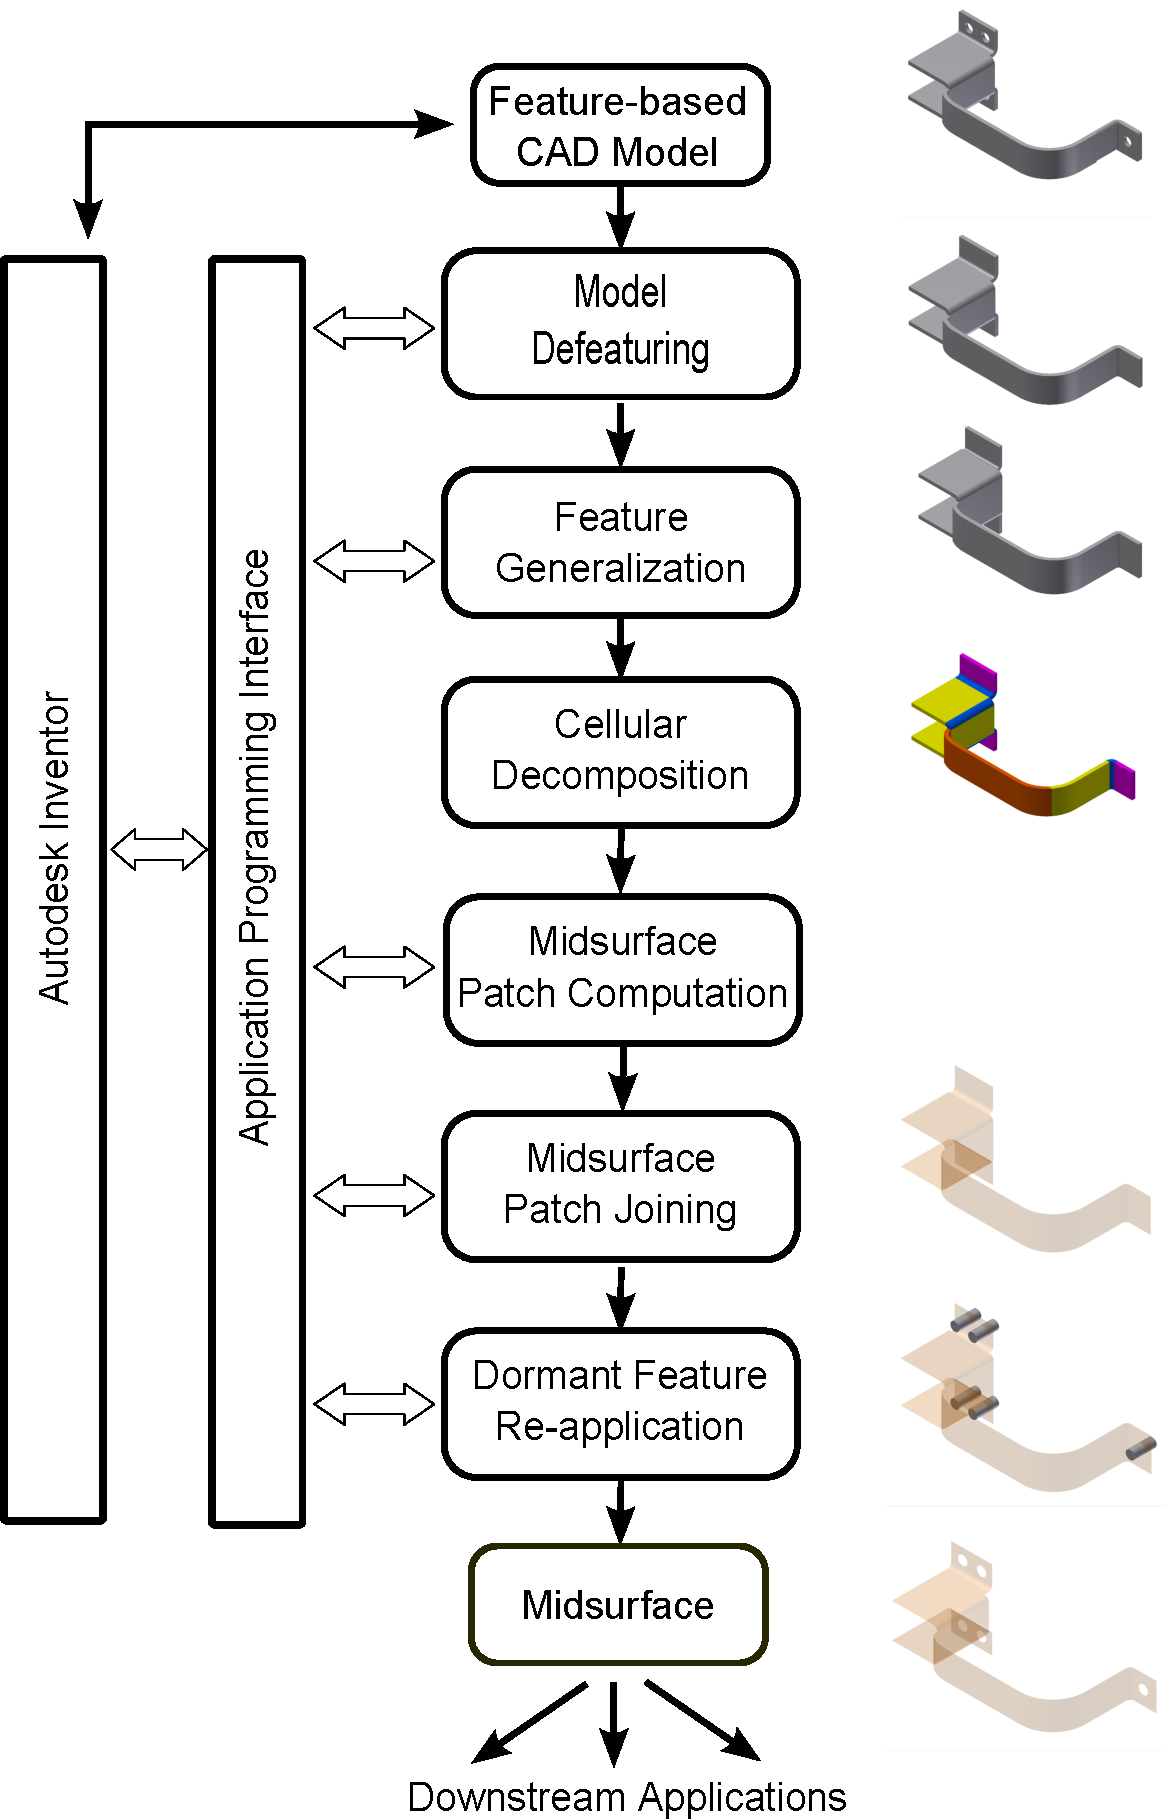
\includegraphics[width=0.62\linewidth]{images/SystemArchitecture_nolabels_7.pdf}
	%\vspace{\abovecaptionskip}
	\caption{Overall System Architecture of \mysystemname}
	\label{fig:proposal:OverallWorkflow}
	\end{figure}
	
%%\bigskip
	
Figure \ref{fig:proposal:OverallWorkflow} shows the architecture, overall work-flow and various constituent modules of the \mysystemname~system. Each module is implemented using Application Programming Interfaces (APIs)  provided by Autodesk Inventor. CAD Models shown at each stage demonstrate the transformation happening to the models. Following list elaborates each of these modules and their workings.
	
\begin{itemize}[noitemsep,topsep=2pt,parsep=2pt,partopsep=2pt]

\item \textbf{Input}:  Input to \mysystemname~is a CAD part model which is built by using a variety of sheet metal features. The model is represented as a feature history tree.

\item \textbf{Model Defeaturing}: This module defeatures the input CAD model by removing irrelevant features. The criterion for deciding relevance is based on newly devised approaches based on sheet metal feature's taxonomy and remnant feature volumes. Apart from these two approaches, in a third approach, relevant but negative features, such as Holes, Cutouts, etc. are also removed after storing their tool-feature-bodies. These features are called as Dormant features. Removal of dormant features further simplifies the model, thus making further midsurface computation stages easier. Once midsurface is computed, the stored dormant feature bodies are re-applied back so that they preserve their impression on the midsurface. Detailed approach of this module is presented in chapter \ref{ch:Defeaturing}.

\todo{[ADDED FOLLOWING PARAGRAPH AS SUGGESTED. IF IT HAS BECOME TOO BIG WE CAN PRUNE IT]}

\item \textbf{Feature Generalization}: A typical sheet metal part is modeled through a variety of sheet metal features with feature parameters. Though these features meaningfully represent the context of sheet metal domain their sheer number and variety can make the midsurface generation a complex task. \replaced{Simplifying them further will obviously make midsurface computation easier and quicker.}{still the remaining number of features could be substantial. It is obvious that simpler is the feature tree and features proper, midsurface computation is easier and quicker.} This module, with a set of algorithms transforms the actual feature tree of the model into the one represented by very basic and fundamental modeling features such as Extrude, Revolve, Sweep and Loft, along with boolean operations. \deleted{As such, Extrude, Revolve and Sweep are specialized forms of the Loft feature only. These variations, called Loft equivalents, are primarily referred in the context in which they were modeled. The output CAD model thus essentially gets represented as modeling function of {\bf A}ffine transformation, {\bf B}ooleans,  {\bf L}oft-equivalents and {\bf E}ntities, in short, known as, $\mathcal{ABLE}$ representation.}  Since such a model essentially contains only Loft-equivalent features combined with boolean operations, the complexity of the midsurface computation drastically reduces. Detailed approach and methodology of this module is presented in chapter \ref{ch:Abstraction}.

\item \textbf{Cellular Decomposition}: This module takes input a simplified and generalized feature based CAD model and decomposes it into finite number of manageable volumes called ``cells''. These cells typically represent primitive shapes of solid, each with a Loft-equivalent owner feature. The connectivity of these cells is captured in a graph based data structure.  Graph nodes are classified into midsurface patch generating nodes, called as patch nodes and midsurface patch joining nodes called as junction nodes. Cells pointed by patch nodes are called as solid cells. Cells pointed by junction nodes are called as interface cells.

\item \textbf{Midsurface Computation}: Midsurface patches are generated for each solid cell, either by offsetting the profile face or by first generating midcurve from the profile followed by lofting it. Incident midsurface patches are subsequently joined within interface cells. Details of the algorithms are presented in Chapter~\ref{ch:Midsurface}.

\todo{Review comment: Do not give these details here. Follow the pattern at previous module an provide an overview of what is input the processing and output. Essentially here we need to provide theme and not details. [REMOVED DETAILS]}

\item \textbf{Dormant Feature Re-application}: Dormant feature tool bodies are reapplied to bring back the relevant negative features onto the midsurface. 

\item \textbf{Validation}: The output midsurface is validated by newly devised approach topological validation, in which predicted topological entities of midsurface are matched with the topological entities of the actual output midsurface. Any mismatch tells the presence of errors such as missing faces, gaps, etc. This approach is only a theoretical proposal and has not been  implemented in \mysystemname.
\end{itemize}

\section{System Specifications} \label{sec:proposal:sysspecs}

\mysystemname~has been designed and developed in a modular fashion employing Object-Oriented (OO) Programming  methodology. It is implemented using OO programming languages, such as VB.Net and C\#.Net. \mysystemname~interacts with Autodesk Inventor modeler through its published APIs to query and reason the model data as well as to render the output. \deleted{The system extends the Graphical User Interfaces of Autodesk Inventor to introduce midsurface generation capabilities developed in the present research work.}

Prototype implementation has been done on Intel 64 bit processor PC.  Many of the example parts used to demonstrate the concepts, have been borrowed from GrabCAD\textsuperscript{\textregistered} site (http://www.grabcad.com).

\section{Implementation Approach} \label{sec:proposal:implementation}
Autodesk Inventor APIs were chosen for \mysystemname's implementation, because of availability of the student version for free and mature APIs over releases.  Autodesk also provides free technical support. The student version also comes with own in-built CAE module, where the output midsurface can be tested.

CAD APIs are typically used to write custom programs in various ways such as Add-Ins, External programs, etc. \mysystemname~ has built various External programs using APIs.
\todo{[REMOVED THE INVENTOR API FRAMEWORK DIAGRAM S IT WAS NOT VERY RELEVANT TO THE IMPLEMENTED SYSTEM]}
%%The Inventor API program structuring is as follows:
%%
%%	 \begin{figure} [!h]
%%	\centering
%%	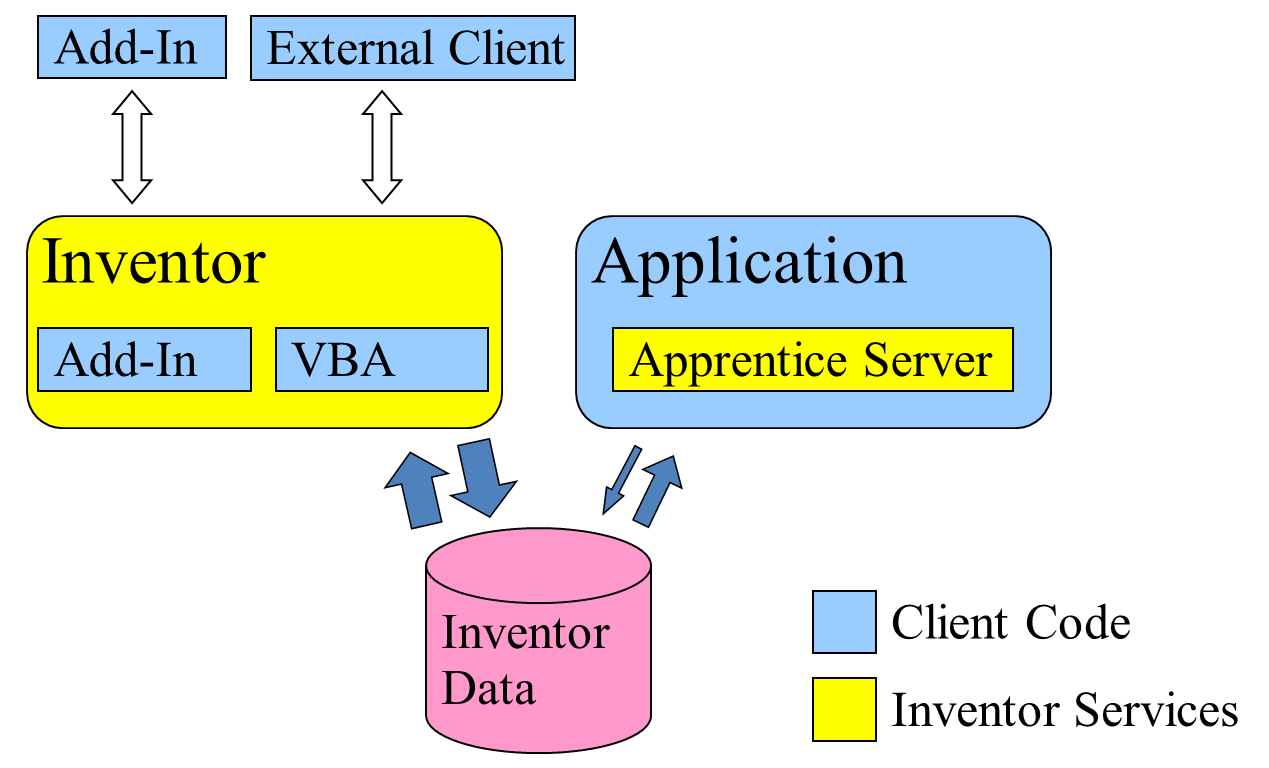
\includegraphics[width=0.9\linewidth]{images/InventorAPI}
%%	%\vspace{\abovecaptionskip}
%%	\caption{Out-of-Process/External VB.Net application }
%%	\label{fig:proposal:InventorAPI}
%%	\end{figure}
Implementation of \mysystemname~consists of neatly encapsulated software modules by using Object Oriented classes, that interact with each other through well defined interfaces. Core and internal algorithms are hidden from other classes to maintain security as well as to facilitate internal changes without disturbing the users of the classes. The modules are as follows:

\begin{itemize}
\item \textbf{Model Defeaturing}: VB.Net OO class Defeaturer encapsulates the logic of iterating over input sheet metal CAD features and removing the irrelevant ones. It exposes only the driver $Run()$ function. This function does the actual defeaturing and shows performance statistics. The defeatured model is saved with ``\_Defeatured'' extension. Tool bodies of dormant features are computed and stored to be used later for reapplication on the midsurface.
\item \textbf{Feature Generalization}: VB.Net OO class Generalizer encapsulates the logic of iterating over ``\_Defeatured' sheet metal CAD features and transforming them into generalized loft equivalents. It exposes only the driver $Run()$ function. The output generalized  $\mathcal{ABLE}$  model is saved with ``\_Able'' extension.
\item \textbf{Cellular Decomposition}: CAD model with ``\_Able'' extension is decomposed into cells, each having Loft-equivalent owner feature(s). Classes such as Graph, Node and Edge are used to populate the graph with each Node pointing to the cells. Edges are formed based on the connectivity between nodes. Nodes have attribute showing whether they are patch generating nodes or junction nodes.  The decomposed model is saved with ``\_Decomposed'' extension.
\item \textbf{Midsurface Computation}:  VB.Net program takes ``\_Decomposed'' extension CAD model and iterates over patch creating nodes of the graph. It computes midsurface by first computing the midcurve of the owner feature's sketch and then lofting it.
\item \textbf{Midcurve Computation}:  Midcurve computation program is called from patch-creation module as mentioned above, by passing sketch as input, resulting into midcurves as output.
\item \textbf{Midsurface joining}: After midsurface patches are ready, the junction nodes join the incident patches. Finally $Stitch$ function is called just to join together already well-placed midsurfaces.
\item \textbf{Dormant Re-application}: Stored dormant tool bodies are re-applied on the midsurface to pierce them through. The output midsurface is saved with ``\_Midsurface'' extension.
\end{itemize}

The output midsurface is then sent for shell meshing for CAE analysis.

%% OO methodology, modular structure, .Net architecture, Inventor external program architecture
%%
%%Following modules are developed, with clear interfaces, making them independent, easy to develop and debug.
%%\begin{itemize}
%%\item \textbf{Defeaturing}: VB.Net program takes Autodesk Inventor \textsuperscript{\textregistered} Sheet metal model and suppresses the irrelevant features.
%%\item \textbf{Abstraction}: VB.Net program takes defeatured model and converts them to Extrude/Revolve/Sweep/Loft
%%\item \textbf{Decomposition}: Splitting of abstracted model is done manually. Each sub-volume is a separate solid having either of Extrude/Revolve/Sweep/Loft as owner feature.
%%\item \textbf{Midsurface}:  VB.Net program takes decomposed solid and computes midsurface patch for each. This module then gets called in computing patches for $sCells$.
%%\item \textbf{Midcurve}:  C\#.Net program takes a polygon as input and computes the midcurve. This module gets called in the ``Midsurface'' module for patch creation.
%%\item \textbf{Midsurface joining}: VB.Net program takes decomposed solids as cells, populates a graph, classifies them into Solid Cells ($sCell$, where Midsurface pacth is generated) and Interface Cells ($iCell$, where connections happen). 
%%\end{itemize}


\section{Scope of System} \label{sec:proposal:scope}
Although Autodesk Inventor exposes most of the functionality via its APIs, it does not do so fully, due to proprietary reasons. So, all the modeling interactions that are possible in the interactive mode are not always available via APIs. This puts some restrictions on the functionality that can be developed using APIs. \deleted{Considering these restrictions the scope of the present research implementation has limited itself to certain sheet metal features and some specific modeling operations only.} It is however noted that those limitations do not anyway dilute the principles and objectives of the research. That is if the CAD modeler later provides the required capabilities through APIs, the research coverage can be extended.

\mysystemname~has been implemented to cover sheet metal feature based CAD model as input. The model is considered to be built using the library of sheet metal features provided by Autodesk Inventor's sheet metal part modeling environment.

\todo{[NEED TO REVISIT AS MANY THINGS ARE DROPED. I HAVE A LIST OF ACTUAL SHEET METAL FEATURES WE WORKED ON. SHOULD I PUT IT HERE?]}

% APIs exposed, their limitations, exact features tackeled, Autodesk specific taxonomy

\section{Overall Working of System} \label{sec:proposal:scope}

Overall working of the \mysystemname~system constitutes the following steps in sequence:
\begin{itemize}
\item The input sheet metal CAD model is either prepared afresh in Autodesk Inventor or already created model is opened in the sheet metal modeling environment.
\item Defeaturing functionally is invoked, which when run, removes all the irrelevant features and stores dormant tool bodies. 
\item Generalization functionality is invoked on the saved defeatured model. Each sheet metal feature gets converted to the corresponding Loft equivalent features, thus forming a generalized CAD model. Shape and size of the model remains as is, only the feature tree gets transformed.
\item Decomposition functionality decomposes the generalized CAD model into list of solid cells. Cells are connected to form a cellular graph. Nodes of the graph are classified as patch nodes and junction nodes. Patch nodes point to solid cells and junction nodes point to interface cells.
\item Midsurface generation module starts computing midsurface patches from solid cells and joins them in the interface cells.
\item Dormant feature tool bodies are re-applied onto the midsurface.
\item The midsurface is validated for topological and geometrical correctness.
\end{itemize}

\todo{[REMOVED THE DIAGRAM AND THE ALGORITHM]}

%%The overall algorithm for the system is:
%%
%%%%%\bigskip
%%
%%\begin{algorithm}[!h]
%%\caption{Feature based midsurface computation}
%%\label{alg_FBDMidsurf}
%%\begin{algorithmic}
%%	\REQUIRE Feature based CAD model  represented by  ($\cup_qF^3$)
%%	\STATE $\cup_wF^3 = feature\_based\_defeaturing(\cup_qF^3)$, where, $w \leq q$
%%	\STATE $\cup_wL^3 = feature\_based\_generalization(\cup_wF^3 )$
%%	\STATE $\cup_kC^3 =feature\_based\_cellular\_decomposition(\cup_wL^3)$, where, $C_i \cap C_j = 0| O_{i,j}^2$
%%	\STATE $G(a, ) = compute\_graph\_nodes(\cup_kC^3)$
%%	\STATE $G(a,b) = find\_overlaps\_generate\_edges(G(a, ))$
%%	\STATE $(sCell,iCell) = categorize\_cells(G(a,b))$
%%%	\IF{ $n_i\rightarrow edges > 2$ \& \ $n_i \rightarrow body \rightarrow is\_thin = true$ \& $O_{i,j}^2$ are adjacent} 
%%%		\STATE $type(n_i) = iCell$ 
%%%	\ELSE
%%%		\STATE $type(n_i) = sCell$
%%%	\ENDIF
%%	\FORALL{$sCell$}
%%		\STATE $\cup_aL^2 = compute\_midsurface\_patch(sCell)$ (Algorithm \ref{alg:midsurfcelljoin:MidsurfsCell})
%%	\ENDFOR
%%	\FORALL{$iCell$}
%%		\STATE $\cup_bL^2 = resolve\_interactions(iCell)$ (Algorithm \ref{alg:midsurfcelljoin:MidsurfiCell})
%%	\ENDFOR
%%	\STATE $\cup_1L^2 = (\cup_aL^2) \cup (\cup_bL^2)$
%%	\STATE $\cup_1L^2 = (\cup_1L^2) - (\cup_{dormant}L^3)$
%%	\RETURN $\cup_1L^2$
%%
%%\end{algorithmic}
%%\end{algorithm}
%%
%%%%\bigskip
%%
%%One of the screen-shots of the working system is presented below:
%%
%%%%\bigskip
%%
%%\begin{minipage}[t]{\linewidth}
%%\begin{tabular}[tb]{@{} p{0.7\linewidth} p{0.25\linewidth}@{}}
%%\adjustbox{valign=t}{
%%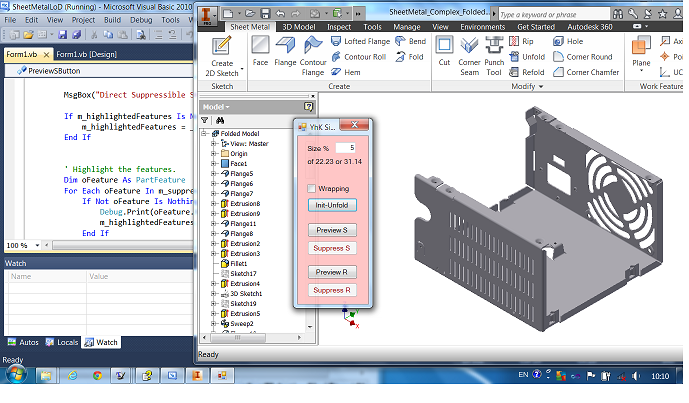
\includegraphics[width=\linewidth]{images/ImplDefeaturingProgram.png}}
%%&
%%\adjustbox{valign=t}{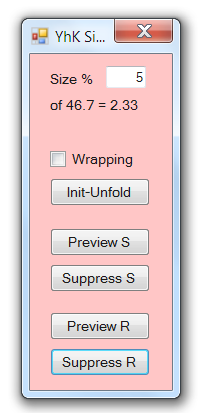
\includegraphics[width=0.8\linewidth]{images/DefeaturingDialog.png}}\\
%%\end{tabular}
%% \captionof{figure}{Screen-shot of the Defeaturing program} \label{fig:proposal:implementation}
%%\end{minipage}
%%
%%%%\bigskip

This chapter has presented an overview of the newly proposed system called \mysystemname~and its architecture. It has provided a brief review of the functional modules, the scope and the system specifications. Finally overall working of \mysystemname~has been outlined in the step-wise manner.

Following chapters present, in detail, the design and development of modules to process the CAD model by various algorithms to finally compute well-connected midsurface with a validation strategy.  


% ----------------------------------------------------------------------------------------------------
\chapter{Defeaturing of Sheet Metal Feature-based CAD Model} \label{ch:Defeaturing}
%% Introduction 
%%	What is this chapter all about? 
%%	What sub-problem or issue is this chapter addressing? 
%%	How does this chapter fit within the overall “story” of the thesis? 
%%The Meat
%%	Rigorous approach to sub-problem, or detailed explanation of issue
%%	Assumptions underlying sub-problem, or complete description of issue
%%	Validation: System design, theory, implementation, graphs, references, …. 
%%Summary
%%	Repeat the highlights of the chapter
%%	Transition sentence that acts as a “teaser” for the next chapter, and how the next chapter fits with the current one


\section{Introduction}

\todo{Review comment: Start with something like ``This chapter provides...'' and give high level view. [DONE]}

\added{The previous chapter presented an overview of the newly proposed system called ``\mysystemname'' and its architecture. This chapter provides details of its first module, called Model Defeaturing, i.e. the algorithms proposed for defeaturing sheet metal feature based CAD model.}

Defeaturing is one of the most popular approaches of simplifying CAD models for CAE analysis. 
\added{CAD models contain various details (or features in case the CAD model is feature based) which are introduced due to requirements of various downstream applications such as CAM, Visualization, etc. Such detailed models are often not needed for CAE, especially for quicker validations at the early stages of design.} Defeaturing is the process of removing irrelevant details or features in the context of application to generate the simplified model, called ``gross shape''\deleted{(Definition \ref{def:grossshape})}. It is the principal shape that ``represents'' the input shape, but with lesser features. In CAE analysis, the finite element mesh generated on the gross shape that is obtained by defeaturing has far lesser number of nodes compared to the original input CAD model. Lesser number of nodes means lesser number of degrees of freedoms (DoFs) for solving the CAE equations, thus lesser computations and quicker analysis results. 

\todo{Review comment: Make this (``Defeaturing is primarily...'') earlier. [BROUGHT HERE]}
\todo{Review comment: Just mention that defeaturing typically helps in significantly reducing DoFs in CAE analysis.[DONE]}

%%\bigskip

	\begin{figure} [!h]
		\centering
		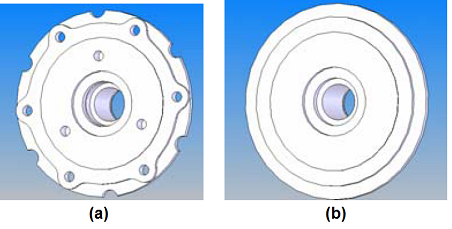
\includegraphics[width=0.7\linewidth]{images/GopalDefeat.png}
		\caption{Gross Shape of Rotor Brake (Source: Gopalkrishnan~\cite{GopalakrishnanSuresh2007})}
		\label{fig:defeaturing:gopaldefeat}
	\end{figure}
	
%%\bigskip

\replaced{Figure  \ref{fig:defeaturing:gopaldefeat}a shows a CAD model of a Rotor Brake part. It has about 50 distinct features and all of them are not relevant for the thermal analysis. After defeaturing, i.e. after removing small holes, depressions, cutouts, etc. the output gross shape is shown in Figure  \ref{fig:defeaturing:gopaldefeat}b.  Gopalakrishnan~\cite{GopalakrishnanSuresh2007} reported that, in this particular example, DoFs got reduced from 150,000 to 25,000 after defeaturing, thereby speeding up the computation significantly.}{Gopalkrishnan~\cite{GopalakrishnanSuresh2007} showed that (Figure \ref{fig:defeaturing:gopaldefeat}) in case of rotor brake model, it has about 50 distinct features and all of them are not relevant for thermal analysis. After computing the ``gross shape'', i.e. removing the irrelevant features, DoFs in CAE analysis got reduced from 150,000 to 25,000, thereby speeding the computation significantly.}

Apart from CAE, gross shapes are also used in shape matching \& retrieval, faster visualizations, hiding proprietary details, quicker transmissions across the networks, etc. Reason being, it is far more efficient to work on the gross shape (which retains the important shape characteristics) than the detailed input CAD model. Thus, due to these advantages, defeaturing is found useful in a wide variety of applications.

The core decision in any defeaturing approach is the criterion of `irrelevance' of a detail or feature in the context of application, which is CAE in this case. For example, for structural CAE analysis, following could be the criteria:

\begin{itemize}[noitemsep,topsep=2pt,parsep=2pt,partopsep=2pt]
\item Remove small fillets \& chamfers. Results of the analysis will show increase in the stresses in the gross shape compared to the original input model. So the results will be conservative and safer for further part design steps.
%\item Remove  Holes will result in an analysis showing lower stresses than the actual case which must somehow be taken into account. \deleted{so that the final design will have sufficient strength.}
\item Do not remove features in the load path and near Boundary Conditions. They are critical to the results and are not to be removed even if they are eligible for removal due to smaller sizes.
\end{itemize}

The present research work takes sheet metal feature-based CAD model as input for computing midsurface. Hypothesis~\ref{hyp:Simplification} which says that the gross shape enhances definitiveness of getting a quality midsurface, is demonstrated in this chapter. Following sections present systematic study of sheet metal feature characteristics to decide the eligibility of some of them for removal.
	
%The research presented here does not take any application-context-specific input data, so it is agnostic to it now, but later, with those inputs available, the method can be tailored to incorporate application-context specific rules as well.
%\footnote{Terms `Defeaturing' and `Simplification', both are used synonymously in this work, unless specified otherwise} 
\section{Need for Defeaturing}\label{sec:defeaturing:need_defeaturing}

\todo{Review coomment: Move this (Section ...) here. [MOVED IT FURTHER IN PROPOSAL AS IT WAS NOT IN THE FLOW]}
\todo{Review comment: Here mention that which of the sheet metal features can be removed without affecting the gross shape. [THESE DETAILS ARE GIVEN A BIT LATER. THE DO NOT SEEM TO FEET AT THIS HIGH LEVEL ``NEED'' SECTION]}

\added{Literature survey Section~\ref{sec:survey:defeat} has reviewed various reported approaches of defeaturing. Subsection~\ref{sec:litsurvey:obsdefeat} concludes that these approaches did not adequately leverage the feature information and to a large extent did not consider application domain.}

The present research focuses on defeaturing \replaced{by leveraging feature information, of sheet metal features based CAD models. Lesser the features the model is built with, retaining the gross shape, easier the computation of midsurface}{for finding the gross shape needed in the computation of the ``Midsurface''}. Following experiment assesses this intuition, which has been formalized in the Hypothesis~\ref{hyp:Simplification} (Chapter~\ref{ch:Survey}).

%\subsection{Effect of defeaturing on the midsurface}
%		Many existing simplification methods recognize small, irrelevant features on a mesh or a solid body first, then remove them to get the simplified (called ``defeatured'')  model. Instead, if a Feature based CAD model is used as an input, then it has the advantage of the availability of ready features, so that the suppression and healing becomes relatively straightforward and robust. In such a feature based defeaturing method, the primary challenge is the identification of the suppressible features. In the past, the suppressibility used to be based on some insufficient criteria, like using full feature parameters, selecting all the negative features, etc. 

%Gross shape is the principal shape that ``represents'' the given shape but with far lesser features. Grossness depends on the size criteria, say, 5\% of the total volume/area. Features having sizes below this are the candidates for suppression.
%%\replaced{Lesser the part is covered with features, easier the computation of the midsurface. Sheet metal features like small Hole, Corner Round, Corner Chamfer, Hems, Rips, etc. can be removed, where as features like Wall, Flange, Bend, are retained.}{With lesser irrelevant details on the input model, the generated midsurface becomes more representative of the original part and the computation becomes robust (small deviations/features in the input do not affect the output in appreciable manner).} 


%%\bigskip

\begin{center}

\begin{tabular}[h]{@{} p{0.17\linewidth} |  p{0.25\linewidth} | p{0.25\linewidth} | p{0.22\linewidth}@{}} \toprule
\textbf{Part and \mbox{actions}} & \textbf{CAD Model} & \textbf{Generated \mbox{Midsurface}} & \textbf{Errors in \mbox{Midsurface}} \\ \midrule

Input model & 
\adjustbox{valign=t}{
 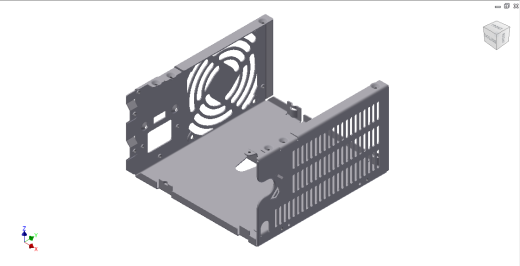
\includegraphics[width=\linewidth]{images/defeatmids_origpart} 
} &

\adjustbox{valign=t}{
 \includegraphics[width=\linewidth]{images/defeatmids_origmids} 
} &

Gaps and missing surfaces
\adjustbox{valign=t}{
 \includegraphics[width=0.4\linewidth, angle=90]{images/defeatmids_origprobs} 
 } 

 \\

Defeaturing of the small irrelevant features. & 
\adjustbox{valign=t}{
 \includegraphics[width=\linewidth]{images/defeatmids_finpart} 
} &

\adjustbox{valign=t}{
 \includegraphics[width=\linewidth]{images/defeatmids_finmids} 
} &

No major errors. Good midsurface. \\

All negative features suppressed. & 
\adjustbox{valign=t}{
 \includegraphics[width=\linewidth]{images/defeatmids_negpart} 
} &

\adjustbox{valign=t}{
 \includegraphics[width=\linewidth]{images/defeatmids_negmids} 
} &

No errors but midsurface lacks important shapes.\\

\bottomrule
\end{tabular}
\captionof{table}{Effect of Defeaturing on Midsurface Generation} \label{tbl:litsurvey:defeatmids}
\end{center}


%%\bigskip


\added{Table~\ref{tbl:litsurvey:defeatmids}  shows results of the experiment of studying the effect of defeaturing on the quality of the midsurface. The first row shows input CAD model and its midsurface computed using a commercial CAD-CAE system. The output midsurface shows various errors such as gaps and missing surfaces, as shown amplified in the picture under `Quality of Midsurface' column. The second row shows the effect of defeaturing, i.e. the removal irrelevant features, such as smaller holes, corner rounds, rips, hems, etc. It does not remove bigger holes, cutouts, flanges, grills, etc. The resultant midsurface does not show any major errors and is of good quality. The third row shows the effect of substantial defeaturing, i.e. removal of all the negative features, even if they are relevant. So all cutouts, patterns, grills, etc. are removed. The output midsurface, although has no gaps, or missing surfaces, lacks presence of the relevant negative features. Such defeaturing needs to be avoided as the midsurface does not represent the correct gross shape. Although this experiment validates the Hypothesis~\ref{hyp:Simplification} to be true, but suggests judicious selection of features for removal.}

\todo{Review comment: So how you have tackled the problem? write 2-3 lines on high level and mention that following section will provide details about the approach. [DONE]}

\added{The present research work, however, proposes use of the substantial defeaturing approach, i.e. the third row shown in Table~\ref{tbl:litsurvey:defeatmids}. Removal of  all the negative features simplifies the computation of midsurface to a large extent. The proposed approach overcomes the problem of missing relevant negative features on midsurface, by storing the tool bodies of those negative relevant features and bringing them back after computing the midsurface for piercing into it. With this arrangement, computing midsurface becomes easier and the output midsurface is not devoid of the impressions of relevant negative features.}

\added{Following section proposes a multi-phase approach for computing the `gross shape', which in turn, helps compute a quality midsurface.}

\section{Proposed Approach to Compute Gross Shape} \label{sec:defeaturing:overall_defeaturing}

\deleted{The concept of "gross shape" is subjective and hard to quantify~\cite{LeeLee1998}, but informal definition~\ref{def:grossshape} clarifies the expectation.} 

\todo{Review Comment: What is the purpose of this line? It doesn't reflect in the following. [REMOVED]}

%\begin{mydef}\label{def:grossshape}
%``gross shape'' is the shape arrived after defeaturing suppressible features, which retains the overall shape and characteristics. 
%\end{mydef}
In the context of the present research work, formulating rules for identification of the irrelevant features is the most critical step that affects the output gross shape.  \replaced{Researchers have measured the}{The} relevance of each feature by evaluation metrics~\cite{AdskElectronicsHelp}. 
%%Here is an example of rules for a particular domain, thermal analysis~\cite{AdskElectronicsHelp}: 
%%
%%	\begin{itemize} [noitemsep,topsep=2pt,parsep=2pt,partopsep=2pt]
%%	\item  Suppress all fasteners, related holes unless in critical heat path.
%%	\item  Suppress rip corners, bends and bend reliefs
%%	\item  Suppress gaps where tabs overlap.
%%%	\item  Replace perforation patterns with simple geometry
%%	\end{itemize}
%%

The evaluation metrics proposed in the present research is divided into three criteria, viz. application context-specific criteria, geometric reasoning-based criteria and dormant features criteria.

%%\bigskip

	\begin{figure} [!h]
		\centering
		\includegraphics[width=0.5\linewidth]{images/SystemArchitectureDefeat_4.pdf}
		\caption{Overall Defeaturing Approach}
		\label{fig:defeaturing:OverallDefeaturingProcess}
	\end{figure}
	
%%\bigskip

 Figure~\ref{fig:defeaturing:OverallDefeaturingProcess} shows \added{phase-wise processing of the input sheet metal feature based CAD model by these criteria. Essentially these criteria apply various rules pertaining to application context, geometric reasoning and negative features, respectively. These rules are applied to identify the criticality of the features in the CAD model in the context of midsurface generation and attempts are made to remove not-so-relevant features from it. A threshold value is computed and provided to the overall approach. It denotes the ``size'' below which a feature is considered as irrelevant. The process thus simplifies the CAD model by defeaturing it while maintaining the gross shape intact. The phases of the proposed defeaturing process are explained below.}
	
\todo{Review comment: Directly start with the next section. [DONE]}
	
	\begin{itemize}
	[noitemsep,topsep=2pt,parsep=2pt,partopsep=2pt,leftmargin=*]
	\item \textbf{Phase I - Sheet Metal Taxonomy based}: The sheet metal CAD model feature tree is traversed and the candidate features for suppression are identified based on criteria based on the newly proposed sheet metal features taxonomy. For other domains or applications, this phase can be customized by employing application context specific taxonomies.
	
	\item \textbf{Phase II - Remnant Features}: This phase is generic and starts with the final Brep for identifying the remnant portions of the features. Those whose sizes are below the threshold are identified for suppression. One can customize the threshold based on engineering judgment appropriately.
	
	\item \textbf{Phase III - Dormant Bodies}: In this phase all ``negative'' features, even though they are relevant and thus have not been identified by the above two phases, are selected for removal, temporarily. Before removal, their feature bodies are cached/stored and are later used for re-applying on the output midsurface. 
	\end{itemize}
	

In the system implementing the proposed approach, it is important to note that, during defeaturing, even though the irrelevant features are said to be removed, they are discarded only temporarily and are not deleted permanently so that, in case of failure, they can be brought back and the original input CAD model to that stage can be restored.
 
%%%\begin{figure}[!ht]
%%%\RawFloats
%%\begin{minipage}[c]{0.95\linewidth}
%%    \begin{minipage}[c]{0.53\linewidth}
%%	\begin{itemize}
%%	[noitemsep,topsep=2pt,parsep=2pt,partopsep=2pt,leftmargin=*]
%%	\item \textbf{Phase I - Sheet Metal Taxonomy based}: The sheet metal CAD model feature tree is traversed and the candidate features for suppression are identified based on criteria based on the newly proposed sheet metal features taxonomy. For other domains or applications, this phase can be customized by employing application context specific taxonomies.
%%	
%%	\item \textbf{Phase II - Remnant Features}: This phase is gemeric and starts with the final Brep for identifying the remnant portions of the features. Those whose sizes are below the threshold are identified for suppression. One can customize the threshold based on engineering judgment appropriately.
%%	\end{itemize}
%%    \end{minipage}
%%    \hfill
%%    \begin{minipage}[c]{0.4\linewidth}
%%        \centering
%%        \includegraphics[width=\linewidth]{images/SystemArchitectureDefeat_1}
%%	 \captionof{figure}{Overall Process}
%%        	\label{fig:defeaturing:OverallDefeaturingProcess}           
%%    \end{minipage}
%%
%%\end{minipage}    
%%%\end{figure}

%The combined method (Phase I \& II) is called as ``\textbf{Smarf}'' (\textbf{S}heet \textbf{M}etal and \textbf{R}emnant \textbf{F}eatures). 
Following sections present the algorithms for these phases in details.


\section{Defeaturing Based on Sheet Metal Features \mbox{Taxonomy}}\label{sec:defeaturing:phase1}

CAD model under consideration is built by a number of sheet metal features such as Wall, Flange, Bend, etc. and are represented as a feature tree. This feature tree is traversed and the candidate features for removal are identified based on a criteria using the newly proposed sheet metal features taxonomy.

Figure ~\ref{fig:defeaturing:tax_sm} shows the proposed taxonomy which classifies sheet metal features and suggests their relevance with respect to maintaining the gross shape. In comparison with the other sheet metal features classifications, such as for features recognition~\cite{Gupta2013, Gupta2013a} and process planning~\cite{Kannan2009}, the proposed taxonomy is \replaced{different in a way that the classification is done based on the criticality of a particular feature to the gross shape.}{a novel one since the application context itself is different, and i.e. of finding the gross shape.}
%
%Sheet Metal parts are built using generic solid modeling features as well as some specialized sheet metal features. 
%
\subsection{Sheet Metal Features Taxonomy}\label{sec:defeaturing:phase11}

A thorough analysis of the inputs from various surveys with engineers and experts in the field to gauge relevance of sheet metal features with respect to the gross shape.  Proposed  taxonomy (Figure ~\ref{fig:defeaturing:tax_sm}) is the result of this analysis.

Taxonomy is represented by ``vocabulary'' and ``structure''~\cite{Tessier2011}. It is a scheme to represent and classify features for a particular purpose~\cite{Dartigues2005}.  Figure ~\ref{fig:defeaturing:tax_sm} shows the classification of sheet metal features for the purpose of computing gross shape.


%%\bigskip

%\begin{minipage}[c]{\linewidth}
\begin{center}
\begin{figure} [!h]
\dirtree{%
.1 Sheet Metal Features.
.2 Primary Features.
.3 Face-Wall   \adjustbox{valign=t}{\includegraphics[scale=0.65]{images/InventorWall.png}}.
.3 Flange  \quad \adjustbox{valign=t}{\includegraphics[scale=0.65]{images/InventorFlange.png}}.
.3 Bend   \qquad \adjustbox{valign=t}{\includegraphics[scale=0.65]{images/InventorBend.png}}.
%.3 Loft Flange  \qquad \adjustbox{valign=t}{\includegraphics[scale=0.65]{images/InventorLoftedFlange.png}}.
%.3 Rib \quad \quad  \adjustbox{valign=t}{\includegraphics[height=0.11\linewidth]{images/Feature_Rib.png}}.
.2 Secondary Features.
.3 Stamping  \quad \adjustbox{valign=t}{\includegraphics[scale=0.65]{images/InventorStamping.png}}.
.3 Cutout  \qquad \adjustbox{valign=t}{\includegraphics[scale=0.65]{images/InventorCutout.png}}.
%.3 Fold  \qquad \adjustbox{valign=t}{\includegraphics[scale=0.65]{images/InventorFold.png}}.
%.3 Roll  \qquad \adjustbox{valign=t}{\includegraphics[scale=0.65]{images/InventorRoll.png}}.
.3 Emboss \qquad \adjustbox{valign=t}{\includegraphics[scale=0.65]{images/InventorEmboss.png}}.
%.3 Hem   \quad \qquad \adjustbox{valign=t}{\includegraphics[scale=0.65]{images/InventorHem.png}}.
%.3 Grill \qquad \adjustbox{valign=t}{\includegraphics[scale=0.65]{images/InventorGrill.png}}.
.2 Tertiary Features.
%.3 Chamfer \qquad \adjustbox{valign=t}{\includegraphics[scale=0.65]{images/InventorChamfer.png}}.
%.3 Round  \qquad \adjustbox{valign=t}{\includegraphics[scale=0.65]{images/InventorRound.png}}.
%.3 Thread \qquad \adjustbox{valign=t}{\includegraphics[scale=0.65]{images/InventorThread.png}}.
.3 Lip \qquad \adjustbox{valign=t}{\includegraphics[scale=0.65]{images/InventorLip.png}}.
.3 Rest \qquad \adjustbox{valign=t}{\includegraphics[scale=0.65]{images/InventorRest.png}}.
%.2 Connecting Features.
%.3 Bend   \qquad \adjustbox{valign=t}{\includegraphics[scale=0.65]{images/InventorBend.png}}.
.2 Features Groups.
.3 Mirror \quad  \quad \adjustbox{valign=t}{\includegraphics[scale=0.65]{images/InventorMirror.png}}.
%.3 RectPattern \quad  \adjustbox{valign=t}{\includegraphics[scale=0.65]{images/InventorRectPattern.png}}.
.3 Pattern\quad  \adjustbox{valign=t}{\includegraphics[scale=0.65]{images/InventorCircPattern.png}}.
}
\caption{Sheet Metal Features Taxonomy (Icons source: Autodesk Inventor~\cite{Inventor2014Help})}\label{fig:defeaturing:tax_sm}
\end{figure}
\end{center}

%%\bigskip

%\begin{tabular}[h]{@{} p{0.45\linewidth}  p{0.45\linewidth}@{}} 
%%\begin{minipage}[c]{0.98\linewidth}
%%\begin{minipage}[t]{0.5\linewidth}
\begin{itemize}
[noitemsep,topsep=2pt,parsep=2pt,partopsep=2pt, leftmargin=*]
\item \textbf{Primary Features}: These features mainly contribute to the gross shape. Examples are  Face-Wall, Flange, Bend, etc.
%	\begin{itemize} [noitemsep,topsep=2pt,parsep=2pt,partopsep=2pt]
%	\item Face-Wall
%	\item Flange
%	\item Bend
%	\end{itemize}
\item \textbf{Secondary Features}: Relevance of these features is based on the relative size with respect to the size of the whole model. Examples are Stamping, Cutout, Emboss, etc.
%	\begin{itemize} [noitemsep,topsep=2pt,parsep=2pt,partopsep=2pt]
%	\item Stamping
%	\item Cutout
%	\item Emboss 
%	\end{itemize}
	
\item \textbf{Tertiary Features}: These features are irrelevant to the gross shape irrespective of their size relative to the size of the whole model. Examples are Lip, Rest, etc.
%	\begin{itemize} [noitemsep,topsep=2pt,parsep=2pt,partopsep=2pt]
%	\item Lip
%	\item Rest 
%	\end{itemize}
	
%\item \textbf{Connecting Features}: These are not suppressed irrespective of their sizes, as removing them, will create gaps between the sub-shapes of the original part. Lacking these would create gaps, so these are retained irrespective of their relative size, small or large.
%Example is:
%	\begin{itemize} [noitemsep,topsep=2pt,parsep=2pt,partopsep=2pt]
%	\item Bend
%	\end{itemize}
		
\item \textbf{Feature Groups}: These are feature collections. Their relevance is assessed as a collection, similar to the secondary features. Examples are Mirror, Patterns, etc.
%\begin{itemize} [noitemsep,topsep=2pt,parsep=2pt,partopsep=2pt]
%	\item Mirror
%	\item Patterns
%	\end{itemize}
\end{itemize}


		
%
%\begin{minipage}[t]{0.4\linewidth}
%		\includegraphics[width=\linewidth]{images/SheetMetal_taxonomy_2.pdf}
%		\captionof{figure}{Examples of classified types}
%		\label{fig:defeaturing:classification}
%\end{minipage}
%\end{minipage}    


Figure~\ref{fig:defeaturing:tax_sm} shows the proposed taxonomy classifying sheet metal features into categories such as Primary features, Secondary features, Tertiary features and Feature groups, based on their sheet metal domain specific characteristics. For defeaturing, each feature category undergoes its own rule for eligibility for removal during defeaturing process. Those rules are elaborated in detail in Section~\ref{sec:defeaturing:taxonomy}.

%%\bigskip

	\begin{figure} [!h]
		\centering
		\includegraphics[width=0.62\linewidth]{images/SheetMetal_taxonomy_3.pdf}
		\caption{Sheet Metal Features Based on Proposed Taxonomy}
		\label{fig:defeaturing:classification}
	\end{figure}
	
%%\bigskip

Figure~\ref{fig:defeaturing:classification} shows example part with various sheet metal features classified as per the proposed taxonomy. %%Following section details out the defeaturing process using the same classification.

\todo{Review comments: Logic of dormant feature needs to be clearly explained (in the algorithm) Why it is appearing here? [IT HAS BEEN MOVED TO ITS OWN SECTION LATER]}

\todo{Review Comments: Explain these steps with figure. [DONE]. Give figures for what is resultant model after processing primary then model after processing secondary and then tertiary. [IMPLEMENTATION IS DONE IN A SINGLE LOOP. WILL NEED TO RE-FACTOR SO THAT SEPARATE OUTPUTS CAN BE COLLECTED. WILL TRY THIS LATER]}

\subsection{Defeaturing Algorithm Based on Sheet Metal Features \mbox{Taxonomy}} \label{sec:defeaturing:taxonomy}

This subsection details the steps used to identify the removable sheet metal features based on the taxonomy proposed in Section~\ref{sec:defeaturing:phase11}. 
\todo{Review comment: What is threshold? Who defines it, what is the typical value you have found after experimenting? [ADDED EXPLANATION]}
Threshold value is computed based on the experimentations done~\cite{YogeshCADandA2016} to assess the effect of different threshold values on the quality of resultant midsurface output. Parameter $D$, which is used as a size criteria for deciding irrelevance of a feature, is defined as threshold \%age ($p$) of the size of the CAD model. Size of the CAD model can be defined in multiple ways, such as, size of Bounding Box, volume, etc. Bounding box as a measure of size, is quick to compute but not accurate. Volume is more accurate than Bounding box but is compute intensive, especially for Brep based CAD model, where the model is composed of faces. Sum of areas of the faces is both, reasonably accurate and easier to compute the size. Thus the present research measures size of the model as sum of the areas of all the faces. The \%age value for threshold is typically based on expertize, application context and engineering judgment. Various experiments were conduced to correlate effect of \%age value of threshold on the gross shapes. Table \ref{tbl:litsurvey:defeatmids} summarizes the results and more details are presented in Appendix~\ref{appendix:threshold}. Based on those experiments typical threshold values used in the present research work are 5-10\%.

Defeaturing rules based on sheet metal features taxonomy are enumerated below:
\begin{enumerate}
[noitemsep,topsep=2pt,parsep=2pt,partopsep=2pt, leftmargin=*]
\item \textbf{Primary Features}: Not removed as these features mainly contribute to the gross shape. Examples are  Face-Wall, Flange, Bend, etc.
%	\begin{itemize} [noitemsep,topsep=2pt,parsep=2pt,partopsep=2pt]
%	\item Face-Wall
%	\item Flange
%	\item Bend
%	\end{itemize}
\item \textbf{Secondary Features}: Are removed based on the relative size with respect to the size of the whole model. Features smaller than the threshold are removed, whereas bigger ones are retained.
%	\begin{itemize} [noitemsep,topsep=2pt,parsep=2pt,partopsep=2pt]
%	\item Stamping
%	\item Cutout
%	\item Emboss 
%	\end{itemize}
	
\item \textbf{Tertiary Features}: Are removed irrespective of their size relative to the size of the whole model. 
%	\begin{itemize} [noitemsep,topsep=2pt,parsep=2pt,partopsep=2pt]
%	\item Lip
%	\item Rest 
%	\end{itemize}
	
%\item \textbf{Connecting Features}: These are not suppressed irrespective of their sizes, as removing them, will create gaps between the sub-shapes of the original part. Lacking these would create gaps, so these are retained irrespective of their relative size, small or large.
%Example is:
%	\begin{itemize} [noitemsep,topsep=2pt,parsep=2pt,partopsep=2pt]
%	\item Bend
%	\end{itemize}
		
\item \textbf{Feature Groups}: Are removed based on the collective relative size with respect to the size of the whole model. 
%\begin{itemize} [noitemsep,topsep=2pt,parsep=2pt,partopsep=2pt]
%	\item Mirror
%	\item Patterns
%	\end{itemize}
\end{enumerate}

 	\begin{figure} [!h]
		\centering
		\includegraphics[width=0.62\linewidth]{images/SheetMetal_Ph1_Selection_Annotated_1.pdf}
		\caption{Defeaturing Based on Proposed Taxonomy }\label{fig:defeaturing:actions}
	\end{figure}
	
Figure~\ref{fig:defeaturing:actions} shows an example sheet metal part CAD model, with taxonomy based features categories shown, along with their defeaturing rules. Primary features such as Walls (Faces), Flanges are not removed. Secondary features whose face-size is less than the threshold are removed, but the larger ones are retained. With threshold as 5 \%, holes smaller than 5 \% of the model faces area, such as Hole2 and CornerRounds are selected but not the bigger holes such as Hole1.
 
%%\bigskip
 
%\subsubsection{Algorithm to identify candidate features for de-featuring based on Sheet Metal feature taxonomy:}
\begin{algorithm}[H]
	\caption{Phase I: Defeaturing Sheet Metal Features}
	\label{alg:defeaturing:phase1}
	\begin{algorithmic}[1]
		\REQUIRE A Sheet Metal FCAD model with access to the feature tree
		
%		\WHILE{$nextFace() != null$}
%			\STATE $F_i = currentFace()$
%			\STATE $Area_{face} \quad += F_i \rightarrow area()$
%		\ENDWHILE		
		\STATE $p = getPreDefinedThreshold()$
		\STATE $Area = sumAllFaceAreas()$
		\STATE $D = \frac{p}{100} \times Area$
		\WHILE{$f_i = currentFeature() != null$}
			\IF {$f_i \rightarrow isPrimaryFeature()$}
				\STATE continue
			\ELSIF {$f_i \rightarrow isTertiaryFeature()$}
				\STATE $sl \rightarrow add(f_i)$
			\ELSIF {$f_i \rightarrow isGroupFeature()$}
			  	\IF {$  f_i \rightarrow combinedArea() < D$}
			  		\STATE $sl \rightarrow add(f_i)$
				\ENDIF
			\ELSE
			  	\IF {$f_i \rightarrow area()  < D$}
			  		\STATE $sl \rightarrow add(f_i)$
%				\ELSIF  {$f_i \rightarrow isNegativeFeature()$}
%					\STATE $sl \rightarrow add(f_i)$ //Dormant feature
				\ENDIF				
			\ENDIF
		\ENDWHILE
		\STATE  $sl \rightarrow removeAll()$
		\STATE  $rebuildModel()$
	\end{algorithmic}
\end{algorithm}

%%\bigskip

Following are the steps taken for defeaturing CAD model based on sheet metal features taxonomy. Algorithm~\ref{alg:defeaturing:phase1} presents the same in pseudo-code form.

\begin{enumerate}
[noitemsep,topsep=2pt,parsep=2pt,partopsep=2pt]
\item The threshold \%age value is chosen. The threshold size is the threshold percentage times of the size of the model. The size of the model  is computed as the total of areas of all faces of the model. It is denoted as ``face-size'' of the model. Similarly, size of the feature is denoted as ``face-size of the feature'' and is the sum of area of the faces of the particular feature (Algorithm~\ref{alg:defeaturing:phase1}: lines 1-3).
\item The model feature tree is traversed and the current feature is applied with the defeaturing rules based on the newly proposed taxonomy (Figure~\ref{fig:defeaturing:tax_sm}, Figure~\ref{fig:defeaturing:actions}) (Algorithm~\ref{alg:defeaturing:phase1}: loop 4 to 18). 
\item The Primary features are not selected for removal so get skipped and do not get added to the removable-features list  (Algorithm~\ref{alg:defeaturing:phase1}: lines 5-6).
%\item The features are selected for removal based on the rules  as detailed out in section~\ref{sec:defeaturing:phase11} based on the newly proposed taxonomy (Figure~\ref{fig:defeaturing:tax_sm}). 
\item If the current feature is a ``Tertiary'' feature, then it is added directly to the removable-features list (Algorithm~\ref{alg:defeaturing:phase1}: lines 7-8).
\item If the current feature is a ``Group'' feature, then it's total face-size of the constituent features is checked against the threshold and if it is less then it is added to the removable-features list (Algorithm~\ref{alg:defeaturing:phase1}: lines 9-12).
\item If the current feature is a ``Secondary'' feature, then it's face-size checked against the threshold and if it is less then the feature is added to the removable-features list  (Algorithm~\ref{alg:defeaturing:phase1}: lines 14-16). 

\item Once all the features in the model are traversed, the features in the removable-features list are removed and the model is regenerated (Algorithm~\ref{alg:defeaturing:phase1}: lines 19-20).
%\item The `candidates list' is presented to the user for verification and changes, if necessary. 
%\item Features in the `candidates list' are removed.
%\item The model is regenerated and Defeaturing Effectiveness is computed using Eqn.~\ref{eqn:defeaturing:effectiveness}
%%
%%\item A list  ({\bf $sl$}) initialized to which the suppressible features are added. 
%%\item The model feature tree is traversed and the candidate features for suppression are identified based on a set of heuristic criteria such as ``Primary features are not to be suppressed'', ``Secondary features, if small, are selected'' etc.  (Figure~\ref{fig:defeaturing:actions}).
%%\item The identified features are added to {\bf $sl$}.
%%\item If ``Dormant' processing option is selected, all the negative features, which otherwise would not have qualified for the suppression are selected for suppression and added to  {\bf $sl$} . The bodies associated with these features are computed and cached. These bodies are later used to pierce the resultant Midsurface (Section~\ref{sec:defeature:dormant})
%%\item The {\bf $sl$} is presented to the user for verification and changes, if necessary. 
%%\item Features in  {\bf $sl$} are suppressed.
%%\item The model is regenerated and Defeaturing Effectiveness is computed using Eqn.~\ref{eqn:defeaturing:effectiveness}
\end{enumerate}


%%%\bigskip

%\subsection{Observations}

\todo{Review comment: Instead of Observations section, continue the algorithm section elaborate it wrt example. [DONE]}

\todo{Review commment: Need to explain this figure. [DONE]}

\begin{minipage}[t]{\linewidth}
\begin{tabular}[!h]{@{} p{0.3\linewidth} | p{0.3\linewidth} | p{0.3\linewidth}@{}} \toprule

\textbf{Input to Phase I} & \textbf{Detected Features} & \textbf{Output of Phase I} \\ \midrule

\includegraphics[width=0.92\linewidth]{images/DefeatPhase_I_t1} &
\includegraphics[width=0.98\linewidth]{images/DefeatPhase_I_t2} &
\includegraphics[width=0.99\linewidth]{images/DefeatPhase_I_t3} \\ \midrule

\includegraphics[width=0.98\linewidth]{images/DefeatPhase_I_1} &
\includegraphics[width=0.98\linewidth]{images/DefeatPhase_I_2_new_nolables.pdf} &
\includegraphics[width=0.98\linewidth]{images/DefeatPhase_I_3} \\ \bottomrule

\end{tabular}
\captionof{figure}{Phase I: Defeaturing Based on Feature Taxonomy and Size Threshold Approach}\label{fig:defeaturing:phaseI}
\end{minipage}

Figure~\ref{fig:defeaturing:phaseI} shows the process pictorially. The first column, called ``Input to Phase I'' shows input sheet metal features CAD model of a bracket part, along with its feature tree. The second column, called ``Detected Features'' shows the candidate features selected, such as `Corner Round1', on the model as well as in the feature tree, based on the steps mentioned above (also mentioned in Algorithm~\ref{alg:defeaturing:phase1}).  The third column shows the output of Phase I, showing the model with candidate features removed.

%%\bigskip




%%\bigskip

%\vspace{-3mm}

\todo{Review comment: At the end state what you conclude with this phase I processing. [DONE]}

With the Phase I over, sheet metal domain specific defeaturing is complete. This phase can be further enhanced by either customizing the threshold and/or by incorporating more features in the taxonomy based on further surveys and experimentations. It can be customized further, for different application domains, such as Injection Molding, by incorporating taxonomy specific to those domain. 

Following section details out the Phase II, i.e. defeaturing process based on geometric reasoning.

 %\vspace{-5mm}
 
\section{Defeaturing Based on Geometric Reasoning of CAD Model Features} \label{sec:defeaturing:phase2}

\todo{Review comment: Change title to Geometric reasoning of model features. [DONE. ADDED `CAD']}

The sheet metal feature based CAD models used in the present research work are built using `design-by-features' approach. At each feature step, the feature parameters first generate a feature primitive solid, known as ``tool-body''. Boolean operation is  performed between operands: the existing model at that stage and the tool body. During this operation, some portion of the tool-body-portion gets consumed within the existing model and the remaining portion of the tool body appears as a newly added feature in the CAD model. 


%%\bigskip

 	\begin{figure} [!h]
		\centering
\includegraphics[width=0.62\linewidth,valign=t]{images/Solid_Simple_SmallProtrusion_labels_2.pdf}
		\caption{Remnant and Consumed Portions} \label{fig_remnant}
	\end{figure}
	
%%\bigskip

Figure ~\ref{fig_remnant} shows boolean operation between the existing CAD model denoted by  $M$ and the tool body of feature $f_2$. Some portion of the tool body gets consumed and is merged with the model whereas some portion remains outside. The portion remaining outside is referred as ``remnant feature'' portion. This phase involves the geometric reasoning to identify remnant feature portions on the input Brep CAD model.

Past attempts such as by Russ~\cite{Russ2012}, used full feature tool-body to determine the candidature for removal during defeaturing. This obviously gives incorrect results as the CAD model actually retains only the remnant portion of the feature. Size of only remnant portion should be considered for deciding the candidature for removal. Thus the present research  uses the size of the remnant portion for deciding removal of a feature and the algorithm to do this is presented below.


\subsection{Defeaturing Algorithm Based on Remnant Feature Portions}

%%In the feature based design paradigm, the CAD model is built step-by-step using features at each step.  At $j^{th}$ feature ($f_j$), the model built till then is referred as $M_{j-1}$.   Feature parameters are used to compute the ``canonical'' (tool-body) volume first, which is then booleaned to the model built till then. $V_j = volume (f_j)$. $V_j$ is the feature/canonical/tool-body volume of the feature $f_j$. $M_j = M_{j-1} \oplus V_j$. The model moves to the next state $M_j$ by boolean of existing state $M_{j-1}$ with the feature volume $f_j$ i.e. $V_j$.  During this operation, some portion of the canonical volume may get consumed, leaving behind the remaining (remnant) volume in the final solid  (Fig.~\ref{fig_remnant}). $V_j = R_{j} \cup C_j$. Some portion of $V_j$ gets consumed ($C_j$) and some remains ($R_j$). (Fig.~\ref{fig_remnant}). $M_j = M_{j-1} \cup  R_j$ and thus $R_j = M_{j} -   M_{j -1}$ is the remnant feature volume ~\cite{Lee2005}.

%%\begin{figure}[!htb]
%%\centering
%% \includegraphics[width=0.35\linewidth]{images/Solid_Simple_SmallProtrusion.pdf} 
%% \caption{Remnant and Consumed portions of feature volume of  $f_2$}
%% \label{fig:defeaturing:remnant}
%%\end{figure}
%%  
%%Identification of suppressible features based on the feature volume computed from the full feature parameters yield incorrect results as the final shape may not retain the full feature volume. So, this work has devised a novel method  (Algorithm~\ref{alg:defeaturing:phase2}) to find the size of remnant feature volume to be used for deciding the suppressibility  (Fig.~\ref{fig:defeaturing:phaseII}) of the features. This phase starts with the final Brep for identifying the remnant portions of the features. This computation, being geometric in nature, can be generic to many applications, with an option to customize the threshold based on engineering judgment specific to the given application.
%%
%%\subsection{Approach}
%%
The input to this phase is the output CAD model from Phase I. In contrast to phase I, this phase does not involve traversal of the feature tree. Instead, it traverses faces of the final model i.e. the Brep model available at the end of the feature tree. As these faces have remained in the model till the end, they are termed as `remnant' faces. The Brep CAD solid model is termed as `final body'. Whenever a feature is added, it adds new faces to the existing Brep model. These new faces store information of the feature which created it, which is termed as the ``owner feature''. The owner feature information is stored on all faces of the Brep as attributes, typically referred as ``origination info''.

The intent of this phase is to group all the remnant faces belonging to a particular feature. This group is termed as `FaceGroup'. Then identify their respective feature owners, and decide their removability on the size of their remnant portions. The size of a FaceGroup can be calculated by various approaches like Influence Volume~\cite{SangHunLee2005} or the union of bounding-boxes, etc. The present work uses summation of the area of the remnant faces as the `Size' criterion and is called ``face-size''. The choice of area as the size criteria is based on ease of computability and reasonable accuracy to represent the remnant portion. 



Following steps present details of the algorithm used to identify remnant faces and thereby remnant features, to be removed based on the remnant portion of the tool body (Figure~\ref{fig_remnant}) (Algorithm~\ref{alg:defeaturing:phase2}).
\todo{Review comment: What is this (clusters table)? its unit, irs rationale, why you use this for what purpose, where are these in figure. [EXPLAINED HERE]}
\todo{Review comment: Give numbers to list items. [DONE]}
\todo{Review comment: A new term (FaceGroup) is coined here which is not explained here. [DONE]}

\begin{enumerate}
[noitemsep,topsep=2pt,parsep=2pt,partopsep=2pt]
\item Remnant faces of the final body are traversed. (Algorithm~\ref{alg:defeaturing:phase2}: loop 1 to 15).  
\item For each remnant face, its owner feature is retrieved (Algorithm~\ref{alg:defeaturing:phase2}: line 2).
\item Existing FaceGroups are searched for matching owner feature.
\item If a match exists, the face is added to that FaceGroup  (Algorithm~\ref{alg:defeaturing:phase2}: lines 4-8).
\item If a match is not found, then a new FaceGroup is created, the remnant face is added to it, it owner feature is set as the owner of the FaceGroup and this new FaceGroup gets appended to the list of FaceGroups  (Algorithm~\ref{alg:defeaturing:phase2}: lines 9-13).

\bigskip

\begin{minipage}{\linewidth}

\begin{minipage}[c]{0.48\linewidth}
\includegraphics[width=0.8\linewidth,valign=t]{images/facegroups_1.pdf}
\captionof{figure}{FaceGroups} \label{fig_clusters}
\end{minipage}
%%\begin{figure}[!h]%[!h]
%%\centering     
%%\subfloat[Remnant and Consumed portions of $f_2$]{\label{fig_remnant}\includegraphics[width=0.5\linewidth,valign=t]{images/Solid_Simple_SmallProtrusion.pdf}} \quad
%%\subfloat[Formation of clusters]{\label{fig_clusters}\includegraphics[width=0.25\linewidth,valign=t]{images/clusters.pdf}}
%%\caption{Phase II: Remnant feature definition, Cluster approach} 
%%\label{fig:defeaturing:phaseII}
%%\end{figure}
\hfill
\begin{minipage}[c]{0.48\linewidth}
\captionof{table}{FaceGroups Details}
\label{tbl_clusters}
\begin{tabular}[h]{@{} p{0.3\linewidth} p{0.25\linewidth} p{0.25\linewidth}@{}} \toprule
\textbf{FaceGroup Id} & \textbf{Face-size ($mm^2$)}& \textbf{Owner Feature}\\ \midrule
FaceGroup$_1$ & 0.25 	&  Extrude$_2$\\
FaceGroup$_2$ & 0.25  & Extrude$_3$\\
FaceGroup$_3$ & 0.125 & Hole$_1$\\ \bottomrule
%$f_{10}, f_{12}, f_{15}, f_{14}$ 	& Cluster$_4$\\ \bottomrule
\end{tabular}
\end{minipage}
\end{minipage}
%%\bigskip

%%\bigskip

Figure~\ref{fig_clusters} shows a schematic of existing Brep CAD model with 3 features booleaned to it. Thick lines are used to represent the remnant faces whereas dotted lines are used to represent the consumed faces. FaceGroup1 and FaceGroup3 are depression features, i.e. negative features, whereas FaceGroup2 is a protrusion feature i.e. a positive feature. In FaceGroup2, $F_{11}$ is a consumed face whereas Faces $F_{10},F_8,F_7$ are the remnant faces. So, FaceGroup2 represents remnant portion of the owner feature Extrude$_3$.

%\item  FaceGroups are formed with same owning features as shown in Figure~\ref{fig_clusters}, where the dotted portions show the consumed feature portions and the circles show the remnant portions. 
\item Face-sizes of the FaceGroups are computed. Table~\ref{tbl_clusters} shows face-size (in $mm^2$) along with owner feature of each FaceGroup.
\item A FaceGroup is removed if its face-size is below the threshold value (Algorithm~\ref{alg:defeaturing:phase2}: lines 16-18). The threshold used is same as the one used in Algorithm~\ref{alg:defeaturing:phase1}: lines1-3.
%%\item The candidates list is presented to the user for verification and changes, if necessary. 
\item Once all the FaceGroups are assessed, removable-features are removed from the feature tree and the model is rebuilt (Algorithm~\ref{alg:defeaturing:phase1}: lines 20-21).
%%\item The model is regenerated and Defeaturing Effectiveness is computed using Eqn.~\ref{eqn:defeaturing:effectiveness}
\end{enumerate} 

\bigskip

\begin{algorithm}[H]
	\caption{Remnant Feature Method}
	\label{alg:defeaturing:phase2}
	\begin{algorithmic}[1]
		\REQUIRE A CAD model with access to the feature tree. 
		\WHILE{$F_i = currentFace() != null$}  
			\STATE $feat = F_i \rightarrow owingFeature()$
			\STATE $addedFlag = false$
			\WHILE {$cl_j = currentFaceGroup() != null$}
				\IF {$cl_j \rightarrow owingFeature() == feat$}
					\STATE  $cl_j \rightarrow add(F_i)$, $addedFlag = true$
				\ENDIF
			\ENDWHILE
			\IF {$addedFlag == false$}
				\STATE  $cl_n = newFaceGroup()$
				\STATE  $cl_n \rightarrow owingFeature() = feat$
				\STATE  $cl_n \rightarrow add(f_i)$
			\ENDIF
		\ENDWHILE
		\WHILE {$cl_k = currentFaceGroup() != null$}
			\IF {$cl_k \rightarrow calculateSize() < D$} %\hspace{40mm} // Threshold D defined in Alg~\ref{alg1}
				\STATE   $sl \rightarrow add(cl_k)$
			\ENDIF			
		\ENDWHILE
		\STATE  $sl \rightarrow removeAll()$
		\STATE  $rebuildModel()$
	\end{algorithmic}
\end{algorithm}


\bigskip

Figure~\ref{fig:defeaturing:phaseII} shows the process pictorially. The first column, called ``Input to Phase II'' shows the sheet metal features CAD model of a bracket part partially defeatured in the Phase I,  along with its feature tree. The second column, called ``Detected Features'' shows the candidate features selected, such as Holes, on the model as well as in the feature tree, based on Algorithm~\ref{alg:defeaturing:phase2}. The Hole is made by cutting a cylinder like tool body. This tool body's dimensions are big enough to disqualify it from removal. But the remnant faces in the model are small enough to qualify this feature for removal. Third column shows the output of Phase II, showing the model with candidate features removed.
%\subsection{Observations}

\bigskip

\begin{minipage}[t]{\linewidth}
\begin{tabular}[h]{@{} p{0.3\linewidth} | p{0.3\linewidth} |  p{0.3\linewidth}@{}} \toprule

\textbf{Input to Phase II} & \textbf{Detected Features} & \textbf{Output of Phase II} \\ \midrule

\includegraphics[width=0.92\linewidth]{images/DefeatPhase_II_t1} &
\includegraphics[width=0.98\linewidth]{images/DefeatPhase_II_t2} &
\includegraphics[width=0.99\linewidth]{images/DefeatPhase_II_t3} \\ \midrule

\includegraphics[width=0.98\linewidth]{images/DefeatPhase_I_3} &
\includegraphics[width=0.92\linewidth]{images/DefeatPhase_II_2_new_wlables.pdf} &
\includegraphics[width=0.98\linewidth]{images/DefeatPhase_II_3} \\ \bottomrule

\end{tabular}
\captionof{figure}{Phase II: Defeaturing Based on Remnant Feature Approach}\label{fig:defeaturing:phaseII}
\end{minipage}

\todo{Review comments: Drop this (observations) section. Continue previous section with elaborate explanation wrt figure. [DONE. ALSO: NEED TO IMPROVE FIGURE AND COMMENTARY. CURRENTLY FUZZY]}






\todo{Review comments: change column names. [THINKING OF ALTERNATIVES]}

%%\bigskip



%%\bigskip

After the first two phases, the given example of bracket model shows 50\% reduction in the number of features and 17\% reduction in the number of faces, at 5\% threshold value. The resulting gross shape has retained all important features necessary for the computation of a quality midsurface.

\section{Defeaturing Based on Dormant Feature Tool-bodies}\label{sec:defeature:dormant}

\todo{Review comment; Change title to bulk features. [NOT CHANGING THE TITLE AS OF NOW TO `DEFEATURING BASED ON BULK FEATURE REMOVAL' AS I AM NOT GETTING ITS MEANING. IN THE PARA, I AM TREATING `BULK' AS `LARGE'.]}

Bulk negative features, such as large Holes, Cutouts can be potentially problematic in further processes used in the midsurface computation, such as feature generalization (Chapter~\ref{ch:Abstraction}) and cellular decomposition (Chapter~\ref{ch:Midsurface}). But they can not be removed because they are necessary constituent of the gross shape. 

\todo{Review comment: First provide rationale as to why some features rather bulk in size need to be mad dormant rather than defeatured. [DONE]}

The results shown in Table~\ref{tbl:litsurvey:defeatmids} demonstrate that removal of negative features, even though they are relevant, can help computation of midsurface. But the drawback is, these features, being relevant would be missing on the midsurface. The present research work proposes to gain the computational advantage but at the same time does not want to loose the relevant features. This proposed approach is called as the Dormant Features approach. In this approach, relevant negative features are removed temporarily, but while doing so their feature bodies (called ``tool-bodies'') are preserved for later usage. After computing midsurface from such highly defeatured model, the preserved tool bodies are brought back and are re-applied on the midsurface. Thus, effect of those important, relevant negative features on midsurface is not lost. However temporary removal does substantially simplify the model which make midsurface computation quite convenient. Following section elaborates Phase III, the dormant features approach.


%\subsection{Approach}\label{sec:defeature:dormantapproach}
\subsection{Defeaturing Algorithm Based on Dormant Features}\label{sec:defeature:dormantalgo}

\todo{Review comment: What is the strategy to identity such features?. [ADDED]}

At this stage, Phases I and II are already over. All the small, irrelevant features are already removed. All the remaining features now, are the relevant features. These can include the negative features as well. In the steps mentioned below, in-spite of being relevant, the large negative features are temporarily removed, after storing their tool bodies. These bodies are kept dormant to be used later for piercing on the midsurface. Algorithm~\ref{alg:defeaturing:phase3} presents pseudo code of the approach and has been listed below: 

\bigskip


\begin{algorithm}[H]
	\caption{Phase III: Dormant Features Identification}
	\label{alg:defeaturing:phase3}
	\begin{algorithmic}[1]
		\REQUIRE A Sheet Metal FCAD model with access to the feature tree
		
%		\WHILE{$nextFace() != null$}
%			\STATE $F_i = currentFace()$
%			\STATE $Area_{face} \quad += F_i \rightarrow area()$
%		\ENDWHILE		
		\WHILE{$f_i = currentFeature() != null$}
			\IF {$f_i \rightarrow isNegativeFeature()$}
				\STATE $b_i = computeToolBody(f_i)$
				\STATE $bl \rightarrow add(b_i)$
				\STATE $sl \rightarrow add(f_i)$
			\ENDIF
		\ENDWHILE
		\STATE  $sl \rightarrow removeAll()$
		\STATE  $rebuildModel()$
	\end{algorithmic}
\end{algorithm}

\bigskip

\todo{Review comment: You are not giving any sense of being dormant here. [ADDED, BOTH, HERE AND IN ALGO]}

\begin{enumerate}
[noitemsep,topsep=2pt,parsep=2pt,partopsep=2pt]
\item The input CAD model feature tree is traversed (Algorithm~\ref{alg:defeaturing:phase3}: loop 1 to 7). 
\item  The current feature is tested if it is a negative feature, like Hole, Cutout, Extrude with subtractive boolean, etc. (Algorithm~\ref{alg:defeaturing:phase3} line: 2). 
\item The tool body is computed using its feature parameters (Algorithm~\ref{alg:defeaturing:phase3} line: 3). 
\item The tool-body is stored in a list (Algorithm~\ref{alg:defeaturing:phase3} line: 4). 
\item The current feature is added to list for removal (Algorithm~\ref{alg:defeaturing:phase3} line: 5). 
\item Once all the features in the feature tree are traversed, the features from candidate features list are removed and the CAD model is rebuilt (Algorithm~\ref{alg:defeaturing:phase3}: lines 8-9).
\end{enumerate}

%By the deferment of processing dormant features, generating midsurface patches gets simplified as these features are not present during their computation.  
\todo{Review comment: Clearly explain algorithm with figure. [IT SHOWS THE APPLICATION OF DORMANT AND NOT SELECTION. AM NEED TO REPLACE WITH A BETTER FIGURE, IF POSSIBLE]}


%%\bigskip




%%\bigskip
	
%\subsection{Observations}\label{sec:defeature:dormantobs}

%%%%\bigskip
%%
%% 	\begin{figure} [!h]
%%		\centering
%%\includegraphics[width=0.45\linewidth,valign=t]{images/dormant_labels.pdf}
%%		\caption{Re-application of the Dormant Feature Tool-body on Midsurface} \label{fig_dormant}
%%	\end{figure}
%%	
%%%%\bigskip

	\begin{figure}[h!]
	\centering 
	%\includegraphics[width=0.85\linewidth]{images/facepairing}
	\subfloat[Input CAD Model]{\label{fig:midsurfcelljoin:beforedomant}\includegraphics[width=0.5\linewidth,valign=t]{images/UBracket_part}} \hfill
	\subfloat[Semi-Final Midsurface]{\label{fig:midsurfcelljoin:semimids}\includegraphics[width=0.49\linewidth,valign=t]{images/MidsurfBracket}} \hfill
	\subfloat[Dormant Tool Bodies Re-application]{\label{fig:midsurfcelljoin:dormant}\includegraphics[width=0.49\linewidth,valign=t]{images/MidsurfDormantBodies_2}} \hfill
	\subfloat[Final Midsurface]{\label{fig:midsurfcelljoin:finalmids}\includegraphics[width=0.49\linewidth,valign=t]{images/MidsurfAfterDormant}}
	\caption{Re-application of the Dormant Feature Tool-bodies on Midsurface}
	\label{fig_dormant}
	\end{figure}
	
Figure~\ref{fig_dormant} shows reapplication i.e piercing of the dormant feature tool bodies. Figure~\ref{fig:midsurfcelljoin:beforedomant} depicts model before detection of the dormant features. Figure~\ref{fig:midsurfcelljoin:semimids} shows midsurface computed after removal of the dormant features. The cached dormant feature tool bodies are brought back and are re-applied on the midsurface, as shown in Figure~\ref{fig:midsurfcelljoin:dormant}. So, the presence of relevant negative features is made sure in the final midsurface as depicted in Figure~\ref{fig:midsurfcelljoin:finalmids}. Thus ensuring faithful representation of all the prominent features on the midsurface. 
%
%\begin{minipage}{0.95\textwidth}
%\begin{minipage}[c]{0.42\linewidth}
%\includegraphics[width=0.75\linewidth,valign=t]{images/dormant}
%\captionof{figure}{Re-application of the Dormant Feature Tool-body on Midsurface} \label{fig_dormant}
%\end{minipage}
%\hfill
%\begin{minipage}[c]{0.56\linewidth}
%% (Refer example in Section~\ref{sec:results:computation} for more details).
%Stored dormant features' tool bodies are reapplied on the midsurface. More details at Figure~\ref{fig:midsurfcelljoin:midsdorm}.
%\end{minipage}
%
%\end{minipage}

\todo{Review comment: Provide  a paragraph of your comment on what is outcome of these three phases. [DONE]}

Table \ref{tbl:defeaturing:benchmarking} shows a brief comparison of the present research work, as implemented in \mysystemname, with the other defeaturing approaches, such as, by Brian Russ~\cite{Russ2012},  Sungchan Kim et. al~\cite{Kim2005} and Sang Hun Lee~\cite{Lee2005}.

\bigskip
%------------------------------------------------------------------------------------
\begin{minipage}[t]{0.9\linewidth}
  \centering
   \captionof{table}{Comparison of the Present Research with Other Methods}
  \label{tbl:defeaturing:benchmarking}
%  \resizebox{\linewidth}{!}{ 
\begin{longtable}[htp]{@{} p{0.16\linewidth} |p{0.18\linewidth} | p{0.18\linewidth}| p{0.18\linewidth} |p{0.18\linewidth}@{}}
\toprule
\textbf{Methods} & \textbf{Russ~\cite{Russ2012}} &	\textbf{Kim~\cite{Kim2005}} &	\textbf{Lee~\cite{Lee2005}} & \textbf{\mysystemname}\\
\midrule
\textbf{Input} & Features	& Brep	& Features	& Features\\
\midrule
\textbf{Approach} & Suppresses if feature size is less than threshold.&
Wrap-around. Negative volumes removed totally. &
Feature volumes are reordered in sorted manner.&
Suppress based on taxonomy and remnant volumes.\\
\midrule
\textbf{Advantages} & Automatic identification of non-critical features &
 Does not need features; Works on Brep&
 Multiple defeaturing levels possible& More accurate criteria for defeaturing
\\
\midrule
\textbf{Limitations} & Limited to FEM as BC and Load path features are not suppressed. &
Concave edge filling creates odd shapes. Principal shape is lost. &
Due merged Cellular model, update capability is lost forever. &
Taxonomy needs to be updated for new features\\	
\bottomrule
\end{longtable}
%}

\end{minipage}


\bigskip

\added{The comparison indicates that the defeaturing approach presented in this chapter significantly reduces the number of faces in the CAD model thus simplifying it considerably for the purpose of midsurface computation. It, however, still ensures that the gross shape of the input CAD model is retained so that underlying design intent is not lost.}

In summary, Phase I removes features from the input CAD model based on the newly proposed sheet metal features taxonomy. The model gets further simplified in Phase II using remnant feature portions approach. Phase III simplifies the model further by completely removing all the negative features. After completion of all three phases of defeaturing the input sheet metal features CAD model is more or less reduced to its gross shape. This is optimum and effective level of defeaturing. Any further removal of the features will disturb the original gross shape intent.

Following section presents a newly proposed measure to assess the effectiveness of the defeaturing process.

\section{Effectiveness of Defeaturing}\label{sec:defeaturing:effectiveness}

\todo{Review comment: Not clear whether these are existing approaches. [THESE ARE EXISTING APPROACHES]}

Effectiveness of the defeaturing process is computed using a wide variety of methods\added{, such as quantitative reduction, MAT, Mesh based, etc.} They can be classified into input-based and output-based methods. In the input-based method, engineering judgment is used to set the initial defeaturing parameters, such as, size threshold, feature taxonomy, etc. and the output resulted is considered as the valid~\cite{MobleyCarrollCanann1998}. In the output-based method, some initial defeaturing parameters are set and the output is assessed against predefined benchmarks, such as, reduction in volume or number of faces or features, etc. The process is repeated till the benchmarks are  achieved. 

In the present research, the input-based method is used to assess the effectiveness of defeaturing. It is computed by measuring {\bf Percentage reduction in the number of faces}. Measurements are done before and after a particular defeaturing phase. More the percentage, more effective is the defeaturing process. A measure of reduction in number of features can also be used in place of faces to form another criterion for assessing the effectiveness. The present research work collects following parameters to compute the effectiveness:

\todo{Review comments: Rename Phase I, II. [RETAINED THESE NAMES, AS THEIR MEANING IS EXPLAINED IN PARAGRAPH ABOVE]}

	\begin{enumerate}
	[noitemsep,topsep=2pt,parsep=2pt,partopsep=2pt]
%	\item Total area of the Faces ($aF$)  ($mm^2$) 
%	\item Threshold size is some (say, 5 percent) of $aF$ ($sP$ $mm^2$)
	\item Total number of the faces in the original part ($nF$)
%	\item Number of sheet metal features suppressed in Phase I ($nS$)
	%\item Time spent in detecting the suppressible features in Phase I ($tS$ sec) 
%	\item Number of faces remaining in the model after Phase I ($mF$)
%	\item Number of \deleted{generic} features suppressed in Phase II ($nR$)
	%\item Time spent in detecting the suppressible features in Phase II ($tR$ sec)	
	\item Number of faces remaining in the model after defeaturing ($rF$)
	\item Defeaturing effectiveness ($pR$) (\%)
	\begin{equation}\label{eqn:defeaturing:effectiveness}  pR = (1 - \frac{rF}{nF}) \times 100\end{equation}
	\end{enumerate}

Defeaturing effectiveness ($pR$) gives quick idea of the order of magnitude of defeaturing.

Following section demonstrates efficacy of the proposed defeaturing approach by evaluating it against CAD model of a real-life test part.

\todo{[REMOVED OTHER METHODS. NOT VERY CONVINCING]}

%%Apart from $pR$, there could be some other and more involved criteria that can be used as follows:
%%	\begin{itemize}
%%	[noitemsep,topsep=2pt,parsep=2pt,partopsep=2pt]
%%	\item \textbf{Medial Axis Comparisons}: Medial Axis Transform (MAT~\cite{Ramanathan2004}) is a skeletal representation of a model. Model, with lots of details will typically generate MAT with branches at the location of details, whereas a simplified model, i.e. without numerous detauils, will not have branches at those locations. Figure~\ref{fig_matbranch} shows how MAT of a simple shape and a shape with extra detail differs. So, Comparison of MAT in case of model before and after defeaturing, by comparing branches can give idea about the effectiveness of the defeaturing process.
%%	
%%%%\bigskip
%%
%% 	\begin{figure} [!h]
%%		\centering
%%\includegraphics[width=0.55\linewidth,valign=t]{images/matbranch}
%%		\caption{Introduction of a detail adds a branch in MAT (Source~\cite{Chen1998})} \label{fig_matbranch}
%%	\end{figure}
%%	
%%%%\bigskip	
%%	
%%\todo{[REMOVED MESH COMPARISON. NOT VERY CONVINCING]}	
%%%	\item \textbf{Mesh}: Comparing faceted mesh generated by body defeatured by {\bf Smarf} with the mesh simplified by any benchmark mesh simplification methods can give the effectiveness measure.
%%	\item \textbf{Size}: Comparison of volume of the original and the defeatured model.
%%	\item \textbf{Shape deviation}: Using Part-Compare functionality, maximum deviation between the original and the defeatured, can be calculated. This deviation should be within predefined limits.
%%\end{itemize}



\todo{Review comment: Drop Implementation section. [DONE]}

%----------------------------------------------------------------------------------------------------------------
\section{Examples} \label{sec:defeaturing:results}

\todo{Review comment: Drop Results section. Instead take an illustrative part show how it gets defeatured, finally compute effectiveness. [RETAINED THE SECTION. ADDED THE EXAMPLE]}

This section exemplifies the defeaturing approach on a typical sheet metal part used as ``Electronics Enclosure''.  It is a typical sheet metal casing model used in electronics equipments. 
%%Figure \ref{fig:results:enlosurebenchmark} show the ``Enclosure'' part and its midsurface computed by a commercial application.
%%
%%\def\myfigenlosurebenchmarkcolumnwidth{0.4} %0.466
%%\begin{figure}[!h]
%%\centering     %%% not \center
%%\subfloat[Original Part]{\label{fig:results:originalenclosurepart}\includegraphics[width=\myfigenlosurebenchmarkcolumnwidth\linewidth,valign=t]{images/SheetMetal_Medium_Enclosure_OriginalPart}} \qquad
%%\subfloat[Commercial Application]{\label{fig:results:midsurfbyinventorexnclosure}\includegraphics[width=\myfigenlosurebenchmarkcolumnwidth\linewidth,valign=t]{images/SheetMetal_Medium_Enclosure_InventorMidsurfwithErrors}}
%%\caption{Computation of Midsurface of an Enclosure Model}
%%\label{fig:results:enlosurebenchmark}
%%\end{figure}
%%
%%Quite a few failures are seen, such as disconnected patches, missing midsurface patches etc. Following sections show progress of the part while goring through various modules.


Following are the steps through which defeaturing of ``Enclosure'' happens. The threshold (D) taken here is 5\%.

%\begin{enumerate}
%[noitemsep,topsep=2pt,parsep=2pt,partopsep=2pt]
%\item
%The model has 3 cutouts for components interfacing with outside world, letter embossing, a chute for wires and holes for fixing bolts.


%%\bigskip

%\begin{figure}[!h]
%\centering     %%% not \center
%\subfloat[Input CAD Model]{\label{fig_enclinputmodel}\includegraphics[width=0.62\linewidth,valign=t]{images/SheetMetal_Medium_Enclosure_OriginalPart}} \qquad
%\subfloat[Feature Tree]{\label{fig_enclinputree}\includegraphics[width=0.32\linewidth,valign=t]{images/SheetMetal_Medium_Enclosure_OriginalTree}}
%\caption{Input CAD Model with Its Feature Tree}
%\label{fig:results:examples1cad}
%\end{figure}


\begin{minipage}{\linewidth}
\begin{minipage}[c]{0.62\linewidth}
\includegraphics[width=\linewidth,valign=t]{images/SheetMetal_Medium_Enclosure_OriginalPart}
%\captionof{figure}{Input CAD Model} \label{fig_enclinputmodel}
\captionof{figure}{Input CAD Model} \label{fig_enclinputmodel}

\bigskip

 Figure \ref{fig_enclinputmodel} shows the input Enclosure part model its corresponding feature tree. It is modeled in Autodesk Inventor using sheet metal features such as Face(Wall), Flange, Bend, Emboss, array of Slots, etc. 
 
\end{minipage}
\hfill
\begin{minipage}[c]{0.32\linewidth}
\includegraphics[width=\linewidth,valign=t]{images/SheetMetal_Medium_Enclosure_OriginalTree}
%\captionof{figure}{Feature Tree} \label{fig_enclinputree}
\end{minipage}

\end{minipage}

%%\bigskip


%\item 

\begin{minipage}{\linewidth}
\begin{minipage}[c]{0.62\linewidth}
\includegraphics[width=\linewidth,valign=t]{images/SheetMetal_Medium_Enclosure_PhaseISelections_2}
%\captionof{figure}{Detected Features Shown in Model} \label{fig_enclph1model}

\captionof{figure}{Features Identified for Removal Shown in Model and Tree} \label{fig_enclph1model}

\bigskip

Figure \ref{fig_enclph1model} shows the selection of irrelevant sheet metal features based on newly proposed sheet metal feature taxonomy. It also shows the bulk negative features as dormant features.  %Figure \ref{fig_enclph1tree} shows the selections in the feature tree.

\end{minipage}
\hfill
\begin{minipage}[c]{0.32\linewidth}
\includegraphics[width=\linewidth,valign=t]{images/SheetMetal_Medium_Enclosure_PhaseISelectionsTree}
%\captionof{figure}{Detected Features Shown in Tree} \label{fig_enclph1tree}
\end{minipage}

\end{minipage}


%\item 

\begin{minipage}{\linewidth}
\begin{minipage}[c]{0.62\linewidth}
\includegraphics[width=\linewidth,valign=t]{images/SheetMetal_Medium_Enclosure_PhaseIISelections_2}

\captionof{figure}{Removal of Features Based on Remnant Feature Approach} \label{fig_enclph2model}

\bigskip

Figure \ref{fig_enclph2model} shows the selection of irrelevant sheet metal features based on remnant feature portions.% Figure \ref{fig_enclph2tree} shows same selections in the feature tree.

\end{minipage}
\begin{minipage}[c]{0.32\linewidth}
\includegraphics[width=\linewidth,valign=t]{images/SheetMetal_Medium_Enclosure_PhaseIISelectionsTree}
%\captionof{figure}{Detected Remnant Features Shown in Tree} \label{fig_enclph2tree}
\end{minipage}

\end{minipage}

%%\bigskip


%\item 
\begin{minipage}{\linewidth}
\begin{minipage}[c]{0.62\linewidth}
\includegraphics[width=\linewidth,valign=t]{images/SheetMetal_Medium_Enclosure_DefeaturedPart}
%\captionof{figure}{Output Gross Shape} \label{fig_Defeaturedmodel}

\captionof{figure}{CAD Model after Full Defeaturing} \label{fig_Defeaturedmodel}

\bigskip

Figure \ref{fig_Defeaturedmodel} shows the result of defeaturing process along with the feature tree. The model has been simplified substantially (\~75\% reduction in the number of faces) while retaining all the principal features thus preserving the gross shape intent.

\end{minipage}
\begin{minipage}[c]{0.32\linewidth}
\includegraphics[width=\linewidth,valign=t]{images/SheetMetal_Medium_Enclosure_DefeaturedTree}
%\captionof{figure}{Features Removed} \label{fig_Defeaturedtree}
\end{minipage}

\end{minipage}

%%\bigskip


%%\def\myfigenlosuredefeaturecolumnwidth{0.95}
%%\def\myfigenlosuredefeatureTreecolumnwidth{0.75}
%%\begin{longtable}[h]{@{} p{0.18\linewidth}  p{0.38\linewidth} p{0.1\linewidth} p{0.2\linewidth}@{}}
%%\toprule
%% & Model & Tree & Explanation \\
%% \midrule
%% 
%%Original/Input &
%%\raisebox{-0.8\height}{\includegraphics[width=\myfigenlosuredefeaturecolumnwidth\linewidth]{images/SheetMetal_Medium_Enclosure_OriginalPart}} &
%%\raisebox{-0.8\height}{\includegraphics[width=\myfigenlosuredefeatureTreecolumnwidth\linewidth]{images/SheetMetal_Medium_Enclosure_OriginalTree}} &
%%
%%The model has 3 cutouts for components interfacing with outside world, letter embossing, a chute for wires and holes for fixing bolts.\\
%%
%%Phase I Selections &
%%\raisebox{-0.8\height}{\includegraphics[width=\myfigenlosuredefeaturecolumnwidth\linewidth]{images/SheetMetal_Medium_Enclosure_PhaseISelections}} &
%%\raisebox{-0.8\height}{\includegraphics[width=\myfigenlosuredefeatureTreecolumnwidth\linewidth]{images/SheetMetal_Medium_Enclosure_PhaseISelectionsTree}} &
%%
%%Small holes, emobssing is chosen based on Sheet Metal feature taxonomy rules (shown red). The green selections are the dormant feature bodies cached.\\
%%
%%Phase II  Selections&
%%\raisebox{-0.8\height}{\includegraphics[width=\myfigenlosuredefeaturecolumnwidth\linewidth]{images/SheetMetal_Medium_Enclosure_PhaseIISelections}} &
%%\raisebox{-0.8\height}{\includegraphics[width=\myfigenlosuredefeatureTreecolumnwidth\linewidth]{images/SheetMetal_Medium_Enclosure_PhaseIISelectionsTree}} &
%%
%%Remnant features got selected in the second phase. \\
%%
%%Defeatured&
%%\raisebox{-0.8\height}{\includegraphics[width=\myfigenlosuredefeaturecolumnwidth\linewidth]{images/SheetMetal_Medium_Enclosure_DefeaturedPart}} &
%%\raisebox{-0.8\height}{\includegraphics[width=\myfigenlosuredefeatureTreecolumnwidth\linewidth]{images/SheetMetal_Medium_Enclosure_DefeaturedTree}} &
%%
%%Most of the unnecessary features are removed and now it retains all the necessary features adequately ``representing''  the gross shape. \\
%%
%%\bottomrule
%%\end{longtable}

%\item 
Effectiveness with 5\% threshold, based on the criterion defined by Eqn. \ref{eqn:defeaturing:effectiveness} is:

\begin{minipage}[c]{0.98\linewidth}
\captionof{table}{Defeaturing Effectiveness Data} \label{tbl_defeatdata}
\begin{longtable}[h]{@{} p{0.3\linewidth} |p{0.3\linewidth}| p{0.3\linewidth} @{}}\toprule
\textbf{Number of Faces Before Defeaturing } & \textbf{Number of Faces {remaining} after Taxonomy-Size Based Defeaturing} & \textbf{Number of Faces {remaining} at the End}\\  \midrule
259 & 104 & 64\\
%  &13 & 8\\
\bottomrule
\end{longtable}

\end{minipage}

\bigskip

\begin{equation}
pR = (1 - \frac{64}{259}) \times 100 = 75.29\%
\label{eqn_case1}
\end{equation}

%\end{enumerate}

%%\bigskip

Table~\ref{tbl_defeatdata} shows the data collected at each phase. It can be seen that even after huge reduction in the number of faces (75\% seen in Eqn.~\ref{eqn_case1}), the overall shape of the enclosure is retained appropriately. This defeatured model is sent for further processing to compute a quality midsurface.

Following section presents conclusions of the process of investigation of problems and proposing solution for defeaturing a sheet metal feature based CAD model.



%%Uniqueness of the present research work with respect to some other relevant approaches \cite{Kannan2009,SangHunLee2005,Russ2012}:
%%	\begin{itemize}
%%	[noitemsep,topsep=2pt,parsep=2pt,partopsep=2pt]
%%	\item Suppressibility rules specific to the domain such as sheet metal feature based design. 
%%	\item Suppressibility rules based on the remnant and not full feature/part volume.
%%	\item No blind suppression of all the negative features or filling-up of the concave volumes.
%%\end{itemize}
%%%%\bigskip

%%Following test cases show the effect of defeaturing on the quality of the midsurface. Size threshold used here is certain percentage of the summation of face-areas of all the faces in the original body.
%%
%%\begin{enumerate}
%%\item Threshold (D) 3\% of the total part size
%%
%%
%%\begin{tabular}[h]{@{} p{0.12\linewidth}  p{0.28\linewidth} p{0.28\linewidth} p{0.28\linewidth}@{}}
%%\toprule
%% & Model & Midsurface & Explanation \\
%% \midrule
%% 
%%Original input &
%%\raisebox{-0.8\height}{\includegraphics[width=0.8\linewidth]{images/defeatresult_perc3_origpart}} &
%%\raisebox{-0.8\height}{\includegraphics[width=0.8\linewidth]{images/defeatresult_perc3_origmids}} &
%%Gaps in the midsurface. Two of the gaps are marked (blue and red).\\
%%
%%Output of Phase I and input to Phase II &
%%\raisebox{-0.8\height}{\includegraphics[width=0.8\linewidth]{images/defeatresult_perc3_ph1part}} &
%%\raisebox{-0.8\height}{\includegraphics[width=0.8\linewidth]{images/defeatresult_perc3_ph1mids}} &
%%Although the number of gaps have reduced (the red gap is filled), but the gaps between the surface patches (blue gap) is still seen. \\
%%
%%Output of Phase II &
%%\raisebox{-0.8\height}{\includegraphics[width=0.8\linewidth]{images/defeatresult_perc3_ph2part}} &
%%\raisebox{-0.8\height}{\includegraphics[width=0.8\linewidth]{images/defeatresult_perc3_ph2mids}} &
%%Some of the gaps (blue gap top portion) are filled and the output is a bit better-connected midsurface. \\
%%
%%\bottomrule
%%\end{tabular}
%%
%%Effectiveness of Smarf with 3\% threshold by Eqn. \ref{eqn:defeaturing:effectiveness} is:
%%
%%\begin{minipage}[c]{0.6\linewidth}
%%\begin{tabular}[h]{@{} p{0.22\linewidth} p{0.18\linewidth} p{0.21\linewidth} p{0.2\linewidth} @{}}\toprule
%%\textbf{Qty} & \textbf{Input} & \textbf{Phase I} & \textbf{Output}\\  \midrule
%%Faces  & 1434 & 610 & 327\\
%%Suppressed  &  & 60 & 30\\
%%\bottomrule
%%\end{tabular}
%%\end{minipage}
%%\begin{minipage}[c]{0.38\linewidth}
%%$pR = (1 - \frac{697}{833}) \times 100 = 16\%$
%%\end{minipage}
%%
%%
%%\item Threshold (D) 5\% of the total part size
%%
%%
%%\begin{tabular}[h]{@{} p{0.12\linewidth}  p{0.28\linewidth} p{0.28\linewidth} p{0.28\linewidth}@{}}
%%\toprule
%% & Model & Midsurface & Explanation \\
%% \midrule
%% 
%%Original input&
%%\raisebox{-0.8\height}{\includegraphics[width=0.8\linewidth]{images/defeatresult_perc5_origpart}} &
%%\raisebox{-0.8\height}{\includegraphics[width=0.8\linewidth]{images/defeatresult_perc5_origmids}} &
%%Gaps in the midsurface. Two of the gaps are marked (blue and red).\\
%%
%%Output of Phase I and input to Phase II &
%%\raisebox{-0.8\height}{\includegraphics[width=0.8\linewidth]{images/defeatresult_perc5_ph1part}} &
%%\raisebox{-0.8\height}{\includegraphics[width=0.8\linewidth]{images/defeatresult_perc5_ph1mids}} &
%%Although the number of missing gaps in the midsurface has reduced (red gap is filled), but the gaps between the surface patches (blue gap) is still seen.\\
%%
%%Output of Phase II &
%%\raisebox{-0.8\height}{\includegraphics[width=0.8\linewidth]{images/defeatresult_perc5_ph2part}} &
%%\raisebox{-0.8\height}{\includegraphics[width=0.8\linewidth]{images/defeatresult_perc5_ph2mids}} &
%%Most of the gaps (blue gap full) are filled and the output is a better-connected midsurface. It retains all the necessary features adequately ``representing''  the gross shape. \\
%%
%%\bottomrule
%%\end{tabular}
%%
%%Effectiveness of Smarf with 5\% threshold by Eqn. \ref{eqn:defeaturing:effectiveness} is:
%%
%%\begin{minipage}[c]{0.6\linewidth}
%%\begin{tabular}[h]{@{} p{0.22\linewidth} p{0.18\linewidth} p{0.21\linewidth} p{0.2\linewidth} @{}}\toprule
%%\textbf{Qty} & \textbf{Input} & \textbf{Phase I} & \textbf{Output}\\  \midrule
%%Faces  & 833 & 772 & 617\\
%%Suppressed  &  &7 & 40\\
%%\bottomrule
%%\end{tabular}
%%\end{minipage}
%%\begin{minipage}[c]{0.38\linewidth}
%%$pR = (1 - \frac{697}{833}) \times 100 = 26\%$
%%\end{minipage}
%%
%%\item Threshold (D) 10\% of the total part size
%%
%%
%%\begin{tabular}[h]{@{} p{0.12\linewidth}  p{0.28\linewidth} p{0.28\linewidth} p{0.28\linewidth}@{}}
%%\toprule
%% & Model & Midsurface & Explanation \\
%% \midrule
%% 
%%Original input  &
%%\raisebox{-0.8\height}{\includegraphics[width=0.8\linewidth]{images/defeatresult_perc10_origpart}} &
%%\raisebox{-0.8\height}{\includegraphics[width=0.8\linewidth]{images/defeatresult_perc10_origmids}} &
%%Gaps in the midsurface. Two of the gaps are marked (blue and red).\\
%%
%%Output of Phase I and input to Phase II &
%%\raisebox{-0.8\height}{\includegraphics[width=0.8\linewidth]{images/defeatresult_perc10_ph1part}} &
%%\raisebox{-0.8\height}{\includegraphics[width=0.8\linewidth]{images/defeatresult_perc10_ph1mids}} &
%%Although the number of missing gaps in the midsurface has reduced (red gap is filled), but the gaps between the surface patches (blue gap) is still seen. \\
%%
%%Output of Phase II &
%%\raisebox{-0.8\height}{\includegraphics[width=0.8\linewidth]{images/defeatresult_perc10_ph2part}} &
%%\raisebox{-0.8\height}{\includegraphics[width=0.8\linewidth]{images/defeatresult_perc10_ph2mids}} &
%%Most of the gaps (blue gap full) are filled. Removal of purple feature could be the domain decision. It retains all the necessary features adequately ``representing''  the gross shape. \\
%%
%%\bottomrule
%%\end{tabular}
%%
%%Effectiveness of Smarf with 10\% threshold by Eqn. \ref{eqn:defeaturing:effectiveness} is:
%%
%%\begin{minipage}[c]{0.6\linewidth}
%%\begin{tabular}[h]{@{} p{0.22\linewidth} p{0.18\linewidth} p{0.21\linewidth} p{0.2\linewidth} @{}}\toprule
%%\textbf{Qty} & \textbf{Input} & \textbf{Phase I} & \textbf{Output}\\  \midrule
%%Faces  & 833 & 715 & 522\\
%%Suppressed  &  &17 & 48\\
%%\bottomrule
%%\end{tabular}
%%\end{minipage}
%%\begin{minipage}[c]{0.38\linewidth}
%%$pR = (1 - \frac{522}{833}) \times 100 = 37\%$
%%\end{minipage}
%%\end{enumerate}
%%
%%The choice of threshold can be set to such a value where midsurface output is well-connected. In the test-cases shown above 10\% appears to be the appropriate value. Increasing the threshold to still higher value results in a well-connected midsurface but it loses the shape characteristics which need to be maintained (Table \ref{tbl:litsurvey:defeatmids}).


\section{Conclusions}

Literature reports that most of the defeaturing algorithms are based on the mesh or solid (Brep) as input. In these cases some kind of feature recognition needs to be performed first and then irrelevant features are identified and removed. With the availability of ready feature information in the feature based CAD models, it has become possible to leverage it for defeaturing purpose effectively. 

The present research proposes to leverage feature information and presents a three phase systematic approach for defeaturing. Each phase employs a different criteria for defeaturing the model. In the first phase, particular sheet metal feature is removed based on its sheet metal characteristics. The second phase uses the size of the remnant portion of a feature for deciding its candidature for removal of the feature. In the third phase all remaining negative features are temporarily removed and their stored tool bodies are brought back for piercing on the computed midsurface. Effectiveness of the defeaturing process is then computed based on the \%age reduction in the number of faces during defeaturing.

\todo{[ADDED ROW FOR ADVANTAGES. CHANGED HEADINGS]}


%%%%%%\bigskip
%%
%%%------------------------------------------------------------------------------------
%%\begin{table}[!h]
%%  \centering
%%   \caption{Comparison of the Present Research with Other Methods}
%%  \label{tbl:defeaturing:benchmarking}
%%  \resizebox{\linewidth}{!}{ 
%%\begin{tabular}[htp]{@{} p{0.19\linewidth} |p{0.19\linewidth} | p{0.20\linewidth}| p{0.19\linewidth} |p{0.20\linewidth}@{}}
%%\toprule
%%\textbf{Methods} & \textbf{Russ \cite{Russ2012}} &	\textbf{Kim \cite{Kim2005}} &	\textbf{Lee \cite{Lee2005}} & \textbf{\mysystemname}\\
%%\midrule
%%\textbf{Input} & Features	& Brep	& Features	& Features\\
%%\midrule
%%\textbf{Approach} & Suppresses if feature size is less than threshold.&
%%Wrap-around. Negative volumes removed totally. &
%%Feature volumes are reordered in sorted manner.&
%%Suppress based on taxonomy and remnant volumes.\\
%%\midrule
%%\textbf{Advantages} & Automatic identification of non-critical features &
%% Does not need features; Works on Brep&
%% Multiple defeaturing levels possible& More accurate criteria for defeaturing
%%\\
%%\midrule
%%\textbf{Limitations} & Limited to FEM as BC and Load path features are not suppressed. &
%%Concave edge filling creates odd shapes. Principal shape is lost. &
%%Due merged Cellular model, update capability is lost forever. &
%%Taxonomy needs to be updated for new features\\	
%%\bottomrule
%%\end{tabular}
%%}
%%
%%\end{table}
%%
%%Table \ref{tbl:defeaturing:benchmarking} shows a brief comparison of the present research work, as implemented in \mysystemname, with the other defeaturing approaches, such as, by Brian Russ~\cite{Russ2012},  Sungchan Kim et. al~\cite{Kim2005} and Sang Hun Lee~\cite{Lee2005}.
%%
%%%%%%\bigskip
%%
%%\added{The comparison indicates that the defeaturing approach presented in this chapter significantly reduces the number of faces in the CAD model thus simplifying it considerably for the purpose of midsurface computation. It, however, still ensures that the gross shape of the input CAD model is retained so that underlying design intent is not lost. The subsequent chapter presents transformation of the features of this gross shape to a generalized feature representation.}

 The subsequent chapter presents transformation of the features of this gross shape to a generalized feature representation.
 
\deleted{Practical example shown in section~\ref{sec:defeaturing:results} demonstrates the efficacy of \mysystemname. It is evident that, even after substantial defeaturing the gross shape computed retains the features essential for computation of a well-connected midsurface.}
%\vspace{-2em}



%----------------------------------------------------------------------------------------------------
\chapter{Transformation of CAD Features to Generalized Feature Representation} \label{ch:Abstraction}
%% Introduction 
%%	What is this chapter all about? 
%%	What sub-problem or issue is this chapter addressing? 
%%	How does this chapter fit within the overall “story” of the thesis? 
%%The Meat
%%	Rigorous approach to sub-problem, or detailed explanation of issue
%%	Assumptions underlying sub-problem, or complete description of issue
%%	Validation: System design, theory, implementation, graphs, references, …. 
%%Summary
%%	Repeat the highlights of the chapter
%%	Transition sentence that acts as a “teaser” for the next chapter, and how the next chapter fits with the current one
	

\section{Introduction}

This chapter presents \replaced{an approach}{process} for feature generalization where sheet metal feature based CAD model is transformed into generalized feature based CAD model. It begins by establishing the need for generalized features and then presents the methodology for building generalized feature based CAD model based on Spatial Grammar technique. \deleted{The proposed model is called as $\mathcal{ABLE}$. Later, transformation of sheet metal feature based CAD model to $\mathcal{ABLE}$ model, is elaborated.} Towards the end, this chapter demonstrates the ease with which midsurface computation can be performed on such CAD model.
\todo{Review comment: First bring out the need of generalized feature representation in the context of midsurface generation. This should be high level. [ADDED THE NEXT PARA]}
\deleted{The present research attempts to use Loft as a generalized feature form to represent CAD features in the sheet metal domain.}
Following section details out the need for generalized feature based CAD model representation.

\section{Need for Generalized Feature Representation}

Feature based CAD models are widely used in development of products from different domains, such as plastics, machining, sheet metal, etc. These domains have their own feature types as per the vocabulary of the domain. For example, sheet metal domain has its own set of features such as Flange, Bend, Slots, Rip, Hem, etc. 

%%\bigskip

	\begin{figure}[!h]
	\centering
	\includegraphics[width=\linewidth]{images/blueboxes}
	\caption{Sheet Metal CAD Model and Feature Tree}
	\label{fig_ariplainpair}
	\end{figure}

	\begin{figure}[!h]
	\centering
	\includegraphics[width=0.5\linewidth]{images/liuFeatures}
	\caption{Sheet Metal Features}
	\label{fig_smtaxonomy}
	\end{figure}
%%
%%\begin{figure}[h!]
%%\centering     %%% not \center
%%\subfloat[Sheet Metal CAD Model and Feature Tree]{\label{fig_ariplainpair}\includegraphics[width=0.63\linewidth]{images/airplanefeatures}} \hfill
%%\subfloat[Sheet Metal Features]{\label{fig_smtaxonomy}\includegraphics[width=0.32\linewidth]{images/liuFeatures}} 
%%\caption{Variety of Sheet Metal Features}
%%  \label{fig:able:variety}
%%\end{figure}

%%\bigskip

\todo{Review comment: Show with an example how too much variety of features can make midsurface generation a complex problem and vis a vis how same model with very generalized primitive features can ease out midsurface generation. [DONE. ADDED EXAMPLE AND Figure \ref{fig_ariplainpair}]}
Figure \ref{fig_ariplainpair} shows a typical sheet metal part along with various features used in its construction such as Face, Flange, Bend, Cutout, etc. Figure \ref{fig_smtaxonomy} shows widely used sheet metal feature types. Actual number of feature types could be in the range of 60-70 for sheet metal domain only~\cite{Inventor2014Help}. Although such diversity of features gives immense flexibility, power to the designers \added{\& modelers} to build desired models, but it can be challenging for downstream applications. So, the existing feature-based midsurface computation approaches need to develop separate computation logic for each of these features~\cite{Robinson2006, Stolt2008, Cao2009}. Large number of feature types thus require huge effort in the design and implementation of midsurface computation algorithm. To avoid this problem, a solution has been proposed in the present research work. It has devised a generic feature form by \replaced{the concept}{process} of generalization. All CAD features are transformed into a smaller set of generalized features, making it easier to write \replaced{the midsurface computation algorithm}{a feature-based algorithm}. 

\todo{Review comment: Why jump to hypothesis 6 without any intro/context. [REMOVED]}
\todo{Review comment: Then mention that ...simplifying the CAD model in terms of generic feature tree that can reduce the complexity of midsurface computation to a great extent. [MENTIONED HERE]}
\todo{Review comment:  Whether this need has been felt earlier by researchers and what was their problem and how they solved it. Introduce Spacial grammar concept here. [DONE]}

\added{The problem of a wide variety of features has been encountered in the past as well. Some researchers used cellular decomposed model to address this for computing midsurface ~\cite{Cao2009}. The CAD model was decomposed into solid cells. The cells were subjected to feature recognition into standardized features such as Extrude~\cite{Boussuge2013a}. Then the midsurface was computed for the Extrudes. Although these approaches work for simple models, they fail on the real-life models due to inability to recognize standard features on decomposed cells. Shapes of cells may not conform to the chosen standardized feature such as Extrude. Another problem was that, during decomposition, the original design intent would get lost which is not recovered by the feature recognition. Thus these approaches have not worked effectively in computing midsurface. The present research addresses these issues as elaborated in the following sections.}

\added{Although the reduction in variety of features helps in reducing the cases to be dealt while writing midsurface algorithm, it would further help if these small set of features themselves be represented by generalized transformations on basic geometric entities. Spatial Grammar~\cite{Stiny1971}, which is widely used in generative design and architecture, etc., describes construction of shapes using transformations of simple geometric entities. These entities and transformations on them are tersely represented by notations known as Spatial Grammar.}
%%In the same context, it proposes and tests hypothesis \ref{hyp:Abstraction}.
%%
%%\begin{myhyp} \label{hyp:abstraction:loft}
%%CAD features can be represented as a single or combination of Loft features  having multiple profiles and a guide curve.
%%\end{myhyp}

%%Lofting, with inputs as $sketches$ and a $guide curve$, is a versatile generic operation. Different geometric shapes can be built by lofting different $sketches$ along with the different $guide curve$s. Table ~\ref{tbl:abstraction:entitiesfeaturesusingable} shows how various entities could be represented using just a $sketch/profile$ and a $guide$. With $Point$ as a fundamental entity, other geometries can be defined by formulating the $sketch$ which is swept along the $guide curve$. 
%%
%%\begin{table}[!htb]
%%\begin{tabular}[h]{@{}p{0.25\linewidth} p{0.18\linewidth} p{0.18\linewidth} p{0.18\linewidth}@{}}
%%\toprule
%%%\backslashbox[1mm]{sketch}{guide} & {\bf line} & {\bf arc} & {\bf curve}\\
%% $sketch\downarrow , guide\rightarrow$   & {\bf line} & {\bf arc} & {\bf curve}\\
%%\midrule
%%{\bf point} & line & arc & curve \\\midrule
%%{\bf line} & plane surf & cylinder surf & ruled surf\\\midrule
%%{\bf arc} & cylinder surf & torus surf & saddle surf \\\midrule
%%{\bf open profile} & ruled surf & circular surf &  free form surf \\\midrule
%%{\bf rectangle} & box & rect torus & rect sweep \\\midrule
%%{\bf circle} & cylinder (surf/solid) & torus (surf/solid)  & tube (surf/solid) \\\midrule
%%{\bf closed profile} & Extrude  (surf/solid) & Revolve (surf/solid) & Sweep (surf/solid) \\\midrule
%%%\bottomrule
%%\end{tabular}
%%\caption{Sweeping based Entities}
%%\label{tbl:abstraction:entitiesfeaturesusingable}
%%\end{table}
%%
%%For example, with $rectangle$ as a $sketch$ and a $line$ as a $guide$ results in a solid $box$ (``Solid'' output option is assumed here. In case of ``surface'' as an output option, open surface box will be created).
%%
%%
%%As the present research focuses on sheet metal parts and one of the peculiarities of them is that they are typically constant thickness models. In this case, Sweep, rather than Loft, is the most appropriate generic form of abstraction. A sweep is a special case of Loft where, instead of multiple profiles, a single profile and a guide curve is specified. Extrude and Revolve are special cases of Sweep, so are used interchangeably to be equivalent forms.

The present research uses Spatial Grammar notations to represent the generalized feature form and has been detailed below. \deleted{Spatial Grammar can be effectively used to represent the neutral form feature representation.}

\section{Related Research}

Following subsections report literature on some of the domains relevant to feature generalization, such as Spatial Grammar and Feature Representation.
% (Definition  \ref{def:formfeature}) representation.  
%
%\begin{mydef}
%\label{def:formfeature}
%Form feature is a local shape (geometric and topological) that has engineering significance.
%\end{mydef}

\subsection{Spatial Grammar Approaches}

\todo{Review comment: Introduce this in earlier section. (or) Drop this [NOT CHANGED AS THE INTRODUCTION LOOKS APPROPRIATE HERE]}

Spatial Grammar is a general term which encompasses various shape definition grammar, like Graph Grammar, Set Grammar etc.~\cite{mckay2012}. Aim of Spatial Grammar is to bring formalism through terse but expressive definitions, validations and generation of new evolutionary shapes. 

Spatial Grammar\deleted{in a generative approach} was formally introduced by Stiny and Gips~\cite{Stiny1971} and is primarily used for exploratory, evolutionary design process. It is defined by set of shapes, labels and rules for geometric transformations. An example rule, say $A \rightarrow B$ first finds a shape with label $A$ and then applies the geometric transformation suggested by the rule and outputs the result $B$. 

\todo{Review Comment; Elaborate further. Don't give any conceptual understanding. [ADDED FIGURE AND FEW LINES EXPLANATION]}

%%\bigskip

	\begin{figure}[!h]
	\centering
	\includegraphics[width=0.62\linewidth]{images/stinyrules.pdf}
	\caption{Shape Grammar Rule (Source: Hoisl~\cite{Hoisl2009})}
	\label{fig:able:StinyRules}
	\end{figure}


%%\bigskip

	
Figure \ref{fig:able:StinyRules}(1) shows a sample rule, say, $r$, where a newer block ($b_1$) is placed on the earlier block  ($b_0$) orthogonally, after matching the marker dots. This rule, when applied successively $n=7$ times, results in the shape shown in Figure \ref{fig:able:StinyRules}(2). The resultant model can be represented by $n \times r(b)$. Thus a shape can be represented by an expressive and terse notation. Using variety of such rules, it is possible to build shapes. Inspite of these advantages its usage in the mainstream design applications appears marred due to complexity of defining and editing the rules.

Hoisl et al.~\cite{Hoisl2009} proposed a Spatial Grammar based system, with implementation in CAD\deleted{for generative solutions}. They used primitives like block, cylinder, cone as initial shapes and proposed use of \replaced{Sweep feature}{{\em sweeping}} to generate different shapes depending on different profiles and guide curves. Boolean operations were used to build more complex shapes. 

CAD Grammar proposed by \added{Deak}~\cite{Deak2006} combined Shape and Graph Grammar to be more useful in Design, Modeling and Manufacturing. He claimed that traditional Shape Grammar could not work well with the CAD primitives\deleted{ and it would be desirable to have such a representation that will work with different CAD systems}.

\added{Moustapha~\cite{Akin2004, Moustapha2004, Hoda2005} developed interactive geometric configuration system based on Shape Grammar for architectural designs. Transformation rules were similar to language grammar rules. Although, with a wide variety of transformations, it was possible to generate different shapes, it lacked one of the key property, i.e. uniqueness. There is no process for recognizing spatially equivalent, yet, notationally different configurations. }

Apart from Spatial Grammar related approaches there have been attempts to devise generalized (also known as `neutral') feature form with which CAD models are built. This is elaborated briefly in the following subsection. %Following subsection elaborates those in brief.

\todo{Review Comment: Survey table not needed. [REMOVED]}

%
%\csvreader[longtable=|p{0.15\linewidth}|p{0.15\linewidth}|p{0.15\linewidth}|p{0.2\linewidth}|p{0.17\linewidth}|p{0.17\linewidth}|,
%    table head=\toprule \bfseries Author & \bfseries Input& \bfseries  Method & \bfseries  Approach& \bfseries  Advantages& \bfseries  Limitations \\ \midrule \endhead,% \bottomrule \endfoot,
%  late after last line=\\\bottomrule,
%  before reading={\catcode`\#=12},after reading={\catcode`\#=6},    
%    late after line=\\\hline]%
%{litsurvey_grammar.csv}{Author=\Author, Input=\Input, Method=\Method, Approach=\Approach, Advantages=\Advantages ,Limitations=\Limitations}%
%{\Author  & \Input&  \Method &\Approach & \Advantages & \Limitations}%


\subsection{Feature Representation Approaches}

A feature-based CAD model is built using features. Each feature adds, modifies, deletes a solid volume, thereby transforming the existing model. So, feature is a similar entity in building a CAD model, as a rule in the Spatial Grammar. Features are specific to applications, such as sheet metal, manufacturing, etc. Due to a large variety of features, developing a generic feature-based algorithm is cumbersome. Many researchers have attempted to either devise a generalized feature form or present feature class hierarchy (taxonomy) so that similar features can be treated similarly in the algorithm. \deleted{A generally accepted definition of a feature is that  it represents shape as well as functionality significant to a particular product life-cycle phase~\cite{Berg2002}.  Features embed application specific high level knowledge and manifest differently as per the context~\cite{mandorli1996}.}


%%\bigskip

	\begin{figure}[!h]
	\centering
	\includegraphics[width=0.5\linewidth]{images/OntologyTessier}
	\caption{Feature Ontology (Source: Tessier~\cite{Tessier2013})}
	\label{fig:litsurvey:Tessier}
	\end{figure}


%%\bigskip

\deleted{Features through use of taxonomy, semantics and ontology  bring formalized knowledge representation which can be leveraged to address problems such as interoperability between CAD system and developing downstream applications such as CAE, CAM etc~\cite{BidarraBronsvoort2000},~\cite{Tessier2011},~\cite{Ma2013}. }
	  
In figure \ref{fig:litsurvey:Tessier} Tessier showed that the generalized feature form can be represented using feature-type, solid body (B-rep) geometry and attributes. 
	  
Middleditch~\cite{Middleditch1997} provided abstract definition for geometric features based on cellular structure, which supported design, manufacturing applications. 

Brunetti~\cite{Brunetti2005} combined parametric modeling with ontological reasoning for application of feature interoperability. His semantic-based shape representations was applicable to different engineering tasks using application specific ontologies.	  

\todo{Review Comment: Survey table and Observations not needed. Instead of these observations have a separate paragraph or a section to explain how shape grammar concept can be leveraged for midsurface problem. How and why it has a potential for the same. has anybody used shape grammar this way? If not say that you have proposed an approach for this. [REMOVED AND ADDED A PARA BELOW]}

%%
%%	
%%\csvreader[longtable=|p{0.15\linewidth}|p{0.15\linewidth}|p{0.15\linewidth}|p{0.2\linewidth}|p{0.17\linewidth}|p{0.17\linewidth}|,
%%    table head=\toprule \bfseries Author & \bfseries Input& \bfseries  Method & \bfseries  Approach& \bfseries  Advantages& \bfseries  Limitations \\ \midrule \endhead,% \bottomrule \endfoot,
%%  late after last line=\\\bottomrule,
%%  before reading={\catcode`\#=12},after reading={\catcode`\#=6},    
%%    late after line=\\\hline]%
%%{litsurvey_featureontology.csv}{Author=\Author, Input=\Input, Method=\Method, Approach=\Approach, Advantages=\Advantages ,Limitations=\Limitations}%
%%{\Author  & \Input&  \Method &\Approach & \Advantages & \Limitations}%

%%\subsection{Observations from Related Approaches}
%%
%%%
%%\begin{itemize}[noitemsep,topsep=2pt,parsep=2pt,partopsep=2pt]
%%	\item In general there has been limited success to the usage of Spatial Grammar in CAD and in the downstream applications, so far, especially for the purpose of neutral {\em feature} definitions.
%%	\item  As this work focuses on thin-walled solids, so naturally scopes itself to work on Sheet Metal features. Use of Spatial Grammar notations to represent scheme of generalized {\em form features} is relatively new and is not widely utilized in the commercial CAD applications. 
%%	\item This work formalizes an approach to  the neutral form-feature representation and later uses it to develop the midsurface computation algorithm.
%%\end{itemize}

\added{From the literature reviewed so far it can be concluded that there has been limited number of attempts to the usage of Spatial Grammar and Feature Generalization, in CAD and its downstream applications, especially for use in feature based algorithms. }

\todo{Review Comment: Spatial grammar and feature generalization do not seem to be connected. Do you want to further report work in spatial grammar or this is a different concept? [BOTH ARE DIFFERENT CONCEPTS BUT MERGED HERE TO PROPOSE ABLE]}
\added{The goal of this module is to represent and transform sheet metal CAD features into generalized feature form, which is devised using a Spatial Grammar approach as elaborated below.}


%% Macro Definitions for Operators used in this file
%\newcommand{\loft}[5]{\ensuremath{\textcolor{magenta}{\Omega{\bf \mathcal{L}}_{#1}^{#2,#3}}[\textcolor{blue}{\{#4\}}\textcolor{red}{(#5)}]}}
%
%\newcommand{\affine}[5]{\ensuremath{\textcolor{magenta}{\Delta{\bf \mathcal{A}}_{#1}^{#2,#3}} [\textcolor{blue}{\{#4\}} \textcolor{red}{(#5)}]}}
%
%\newcommand{\boolop}[5]{\ensuremath{\textcolor{magenta}{\Omega{\bf \mathcal{B}}_{#1}^{#2,#3}}[\textcolor{blue}{\{#4\}} \textcolor{red}{(#5)}]}}
%
%\newcommand{\generic}[7]{\ensuremath{\textcolor{magenta}{#1{\bf \mathcal{#2}}_{#3}^{#4,#5}}[\textcolor{blue}{\{#6\}} \textcolor{red}{(#7)}]}}

%Following subsections explore salient work done so far in the areas relevant to Form Feature Representation.

%%\section{Theoretical Background}

%%Features through use of taxonomy, semantics and ontology  bring formalized knowledge representation which can be leveraged to address problems such as interoperability between CAD system and developing downstream applications such as CAE, CAM etc \cite{BidarraBronsvoort2000}. Ontology defines objects-rules in a structured way so that other domains (once schema is known) can traverse this knowledge. Taxonomy will help define class/object hierarchy. The use of the term formal implies that the ontology is machine-readable, but without being too cryptic for human understanding \cite{Brunetti2005, Gupta2013, Abad}.  By establishing a common language for use and interpretation of information, ontologies allow for efficient and organized exchange and reuse of knowledge.


% Middleditch \cite{Middleditch1997} provided feature abstraction by proposing structure, construction sequence and point-set, so as to separate issues of  solid modeling, feature modeling and constraints. Tessier \cite{Tessier2011, Tessier2013}  presented hybrid ontological approach for full exchange of both feature definition semantics as well as geometric constriction data (Figure \ref{fig:litsurvey:Tessier}), mainly for feature validation.

%	\begin{figure}[!h]
%	\centering
%	\includegraphics[width=0.5\linewidth]{images/OntologyTessier}
%	\caption{Feature Ontology (Source: \cite{Tessier2013})}
%	\label{fig:litsurvey:Tessier}
%	\end{figure}
	
%\subsection{State of the Art}
%
%\csvreader[longtable=|p{0.15\linewidth}|p{0.1\linewidth}|p{0.1\linewidth}|p{0.25\linewidth}|p{0.15\linewidth}|p{0.15\linewidth}|,
%    table head=\toprule \bfseries Author & \bfseries Input& \bfseries  Method & \bfseries  Approach& \bfseries  Advantages& \bfseries  Limitations \\ \midrule \endhead,% \bottomrule \endfoot,
%  late after last line=\\\bottomrule,
%  before reading={\catcode`\#=12},after reading={\catcode`\#=6},    
%    late after line=\\\hline]%
%{../DocsSources/litsurvey_abstraction.csv}{Author=\Author, Input=\Input, Method=\Method, Approach=\Approach, Advantages=\Advantages ,Limitations=\Limitations}%
%{\Author  & \Input&  \Method &\Approach & \Advantages & \Limitations}%
%
%\subsection{Observations}
%
%%
%\begin{itemize}[noitemsep,topsep=2pt,parsep=2pt,partopsep=2pt]
%	\item In general there has been limited success to the usage of Spatial Grammars in CAD and in the downstream applications, so far, especially for the purpose of neutral {\em feature} definitions.
%	\item  As this work focuses on thin-walled solids, so naturally scopes itself to work on Sheet Metal features. Use of Spatial Grammar notations to represent scheme of generalized {\em form features} is relatively new and is not widely utilized in the commercial CAD applications. 
%\end{itemize}


 
 
\section{Proposed CAD Model Representation}\label{sec:abstraction:proposal}

\added{Objective of this section is to present the generalized feature-based CAD model representation, based on Spatial Grammar. As the existing sheet metal feature based CAD model will be transformed in this new representation, it will need to map all the necessary entities and functionalities of any feature based CAD representation. Requirements for the proposed generalized representation are:}

 \todo{Review Comment: There is no context, rationale as to why you want to propose this (Theoretical background). [CONTEXT AND RATIONALE ADDED. THE WHOLE IDEA IS TO PROPOSE A GENERALIZED CAD MODEL REPRESENTATION AND THEN SHOW HOW MIDSURFACE CAN BE COMPUTED FROM IT. IN THE NEW MODEL REPRESENTATION I EXPLAIN HOW ENTITIES, TRANSFORMATIONS, BOOLEANS AND FEATURES ARE REPRESENTED]}
 
\begin{enumerate}%[noitemsep,topsep=2pt,parsep=2pt,partopsep=2pt]
[noitemsep,topsep=2pt,parsep=2pt,partopsep=2pt]

\item Ability to represent entities needed to build the model, such as line, circle, spline, solid, surface, etc.
\item Ability to specify transformations to spatially place the entities, such as translation, rotation, scaling, etc.
\item Ability to specify a generalized feature that can represent actual features in the model.
\item Ability to specify booleans to join or cut the feature with existing parts.  
\end{enumerate}


 
The sections below present such generalized representation in a terse Spatial Grammar like notation, to transform sheet metal feature CAD model. Midsurface algorithms are then developed based on such generalized feature based CAD model.

The proposed representation is loosely based upon Interactive Configuration Exploration  (ICE) scheme developed by Hoda Moustapha \cite{Hoda2005} for generative designs in architectural domain. Although some of the fundamental entities and syntaxes are borrowed from ICE, the present research enhances it substantially to suit Mechanical CAD application and specifically, for the current context of computation of midsurface.
 
 Following subsections give more details about the ICE scheme, then present how entities, transformations, generalized features and booleans are represented in the proposed approach.
 

 \todo{Review Comment: It is very difficult to comprehend this without any example and its relevance to our problem. Terms, mathematical expressions need to be properly explained with their relevance, context, example and what you want to do with this. [ADDING FIGURE AND EXPLANATION]}
 
 %%-------------------------------------------------------------------------------------------------------------------------------------------------------------------------------------
\subsection{Interactive Configuration Exploration (ICE) Scheme} \label{sec:abstraction:ice}

{\em "The ICE notation is a formalism for describing shapes and  configurations,  by  means  of  their  generative  and  relational  structures"} -- Hoda Moustapha \cite{Hoda2005}.  There are two fundamental entities in ICE, one is a {\em point} shown as $\bar{p}$ and another is called {\em Regulator}, which is an abstraction that represents a unit of action like transformation, constraints, relations, etc. A {\em Regulator} is represented as \\



{\generic{category}{R}{instance}{subtype}{dimension}{arguments}{shapes}}\\

	 For example, Figure \ref{fig:abstraction:hodatranslate} shows the Translation regulator. Its ICE representation is shown below:

	\affine{}{T}{1}{\bar{p},line,n}{shape} 
	
\begin{figure}[!h]
\centering \includegraphics[width=0.5\linewidth]{images/hodatranslate} 
\caption{Translation of a Shape}
\label{fig:abstraction:hodatranslate}
\end{figure}

	
	where,
		\begin{itemize}[noitemsep,topsep=0pt,parsep=0pt,partopsep=0pt]
		\item 	\textcolor{black}{$\Delta$} : Transformation category (type)
	     	\item 	\textcolor{black}{${\bf \mathcal{A}}$} : Affine-transformation regulator (type)
		\item  	\textcolor{black}{$^T$}: subtype Translation (type)
		 \item 	\textcolor{black}{$^1$} : dimensionality of output (integer)
	        \item 	\textcolor{black}{ $\bar{p}$} : position (point)
  		\item  	\textcolor{black}{$line$} : linear guide (curve)
		 \item  	\textcolor{black}{$n$} : number, used for copies, scaling, etc. (float)
		 \item  	\textcolor{black}{$shape$} : target (shape)
		\end{itemize}

%		\begin{itemize}[noitemsep,topsep=0pt,parsep=0pt,partopsep=0pt]
%		\item 	\textcolor{magenta}{$\Delta$} : Transformation category (type)
%	     	\item 	\textcolor{magenta}{${\bf \mathcal{A}}$} : Affine-transformation regulator (type)
%		\item  	\textcolor{magenta}{$^T$}: subtype Translation (type)
%		 \item 	\textcolor{magenta}{$^1$} : dimensionality of output (integer)
%	        \item 	\textcolor{blue}{ $\bar{p}$} : position (point)
%  		\item  	\textcolor{blue}{$line$} : linear guide (curve)
%		 \item  	\textcolor{blue}{$n$} : number, used for copies, scaling, etc. (float)
%		 \item  	\textcolor{red}{$shape$} : target (shape)
%		\end{itemize}
%
The example is of a triangular shape, being translated linearly, from a point $p$, along $line$, with $n$ copies made. It acts as a linear-pattern operation of the triangle.

The ICE notation, can be mapped to Spatial Grammar rules typically represented as $\mathbb{A} \rightarrow \mathbb{B}$. In above example, $(shape)$ is the inputs to the rule, which can be mapped to LHS ($\mathbb{A}$) for the matching condition. On this input, transformation rule $\mathbb{A} \rightarrow \mathbb{B}$ is applied, using specified-arguments in the $\{\bar{p},line,n\}$ to generate RHS ($\mathbb{B}$). More details of the ICE schema are in Appendix \ref{appendix:ice}.
%%Notation is further explained below:
%%
%%\begin{itemize}%[noitemsep,topsep=2pt,parsep=2pt,partopsep=2pt]
%%[noitemsep,topsep=2pt,parsep=2pt,partopsep=2pt]
%%
%%	\item {\em Regulators} are in {\bf bold}, {\bf  $\mathcal{R}$} , represents a unit of action
%%	\item \textcolor{red}{\em shapes} are in {\em lowercase}, say, \textcolor{red}{\em circle, sketch}
%%	\item Prefix to a  {\em Regulator} is its {\em category}, like, \\
%%		 \textcolor{magenta}{$\Delta$}	 :  transformations  \\
%%		 \textcolor{magenta}{$\Phi$} 	 :  constraints  \\
%%		 \textcolor{magenta}{$\Psi$}		 :  hierarchies  \\
%%		 \textcolor{magenta}{$\Pi$}		 :  topologies  \\
%%		 \textcolor{magenta}{$\Xi$}		 : variations  \\
%%		 \textcolor{magenta}{$\Omega$}  :  operations
%%
%%	\item Superscripted$^{suffixes}$  indicate  regulator  {\em subtype},  for instance, \textcolor{magenta}{$\Delta C^p$} and  \textcolor{magenta}{$\Delta C^e$}  respectively specify parabolic and elliptical curve regulators
%%
%%	\item Numerical$^{suffixes}$ denote the dimension of the {\em Regulator}, for instance, \textcolor{magenta}{$\Delta M^0$} ,   \textcolor{magenta}{$\Delta M^1$ }, and   \textcolor{magenta}{$\Delta M^2$}, respectively represent a mirror point (0-dimensions), a mirror line (1-dimension) and a mirror plane (2-dimensions)
%%
%%	\item  Subscripted$_{suffixes}$ for {\em Regulators,  shapes} represent  as  indices;  for  example  \textcolor{magenta}{$\Delta T_1$},  and  \textcolor{magenta}{$\Delta T_2$} are  two different instances of {\em Translation Regulators} used in the same configuration.
%%
%%	\item {\em Regulators} can be generative or non-generative.  Generative  regulators (depicted by the presence of the ``n'' parameter)  take  an  input  shape  and  create output  shapes,  while  non-generative  regulators  act  on  the  input  shape.
%%
%%	\item \textcolor{magenta}{$\Delta {\bf T}$}\textcolor{red}{($\bar{s})^{<0><1><2>}$}  is  a  discrete  application  generating disjoint points, while  \textcolor{magenta}{$\Delta  {\bf T}$}\textcolor{red}{($\bar{s})^{<0,1,2>}$}  is a continuous application generating a line.  
%%
%%	\item Key-points ($ e$ : endpoint,   $m$ : midpoint,   $s$ : start-point) To access key-points (such as the midpoint): \textcolor{red}{$ shape_A \langle m_1 \rangle$}, length by \textcolor{red}{$shape_A \langle l \rangle$}
%%\end{itemize}
%%
%%
%%The present research formalizes an approach to  the neutral form-feature representation and later uses it to develop the midsurface computation algorithm.



%Hoisl \cite{Hoisl2012} mentioned that a limited set of shapes can be generated using {\em Sweep} in a generic manner. A {\em Sweep} is an operation where moving a shape (called {\em generator}) along a trajectory (called {\em guide curve}) creates variety of shapes. {\em Sweep}, by its strict meaning, is limited by use of a single sketch. A more generic operation is {\em Loft}, where multiple sketches are joined together, along a guide curve. 
%It is found that most of the primitives like {\em Box, Cylinder, Cone, Torus, Sphere} and operators like {\em Extrude, Revolve, Sweep, Loft}, in their simplistic form, can be modeled using a {\em Loft} operator.  
%
%Similarly, operators like {\em Translation, Rotation, Scaling} can be modeled using one generic {\em Affine Transformation} operator. {\em Pattern, Mirror} can also be modeled using the same by taking an additional argument as {\em number of copies}.
%
%Another set of operators that can be uniquely represented as a single operator are {\em  Boolean} operators. {\em Union, Difference, Intersection} work on one {\em target body} and multiple {\em tool bodies} with a difference of only  'which cells to retain' logic.
%
%Such set of core operators has lots of advantages like:
%\begin{enumerate}
%\item Operators can be agnostics to the CAD applications. CAD applications may call them differently but the kernel calls could be same.
%\item Data interoperability could be easier as operators are few, neutral and standardized.
%\item Algorithms based on them can be easily ported to different applications, e.g. Midsurface Extraction developed on such core operators can then be ported to in any CAD-CAE application honoring them.
%\end{enumerate}
%
%In many CAD applications, operators are presented as a combination, e.g. {\em  Extrude}, apart from parameters such as {\em sketch} and {\em direction-length}, can ask choice of {\em boolean} and {\em draft-angle}. In the representation scheme presented below, internal {\em booleans} are decoupled from the feature and are modeled separately  i.e. {\em Extrude} will create just the {\em tool body} which will be {\em boolean-ed} later.


%\section{Proposed Feature Generalization Approach  ($\mathcal{ABLE}$) }

%%Objective of proposing a new feature representation scheme is to come up with a specific-to-generic mapping of form features in the context of CAD. The representation scheme proposed here is loosely based upon Interactive Configuration Exploration  (ICE) scheme developed by Moustapha \cite{Hoda2005}, for architectural designs. Although some the fundamental entities and syntax are borrowed from ICE, the rest has been enhanced it to suit the mechanical CAD application, such as this research.


%\subsection{Proposed enhancements}

\todo{Review comment: This is your very significant contribution and difficult in domain. You have to be very careful and cautious to explain these terms for the reader to appreciate the contribution. [MADE SPECIFIC]}

%To cater to this demand, the concept of {\em Regulator} from ICE has been modified to have \textcolor{magenta}{Operator}, \textcolor{blue}{Guide} and \textcolor{red}{Shape}. \textcolor{magenta}{Operator} consists of Type-Subtype and dimensionality of the output. \textcolor{blue}{Guide} typically has the guide-curve info. \textcolor{red}{Shape} is the one on which the operation happens.
\todo{Don't give feel of hand picked addition deletions, rather explain your approach. [REMOVED THE SPECIFICS AND EXPLAINING RATIONAL AT RELEVANT PLACES]}
%%Although entities like {\em point}, {\em line} are present in ICE but entities and features pertinent to Mechanical CAD are not present. Also treatment given to primitives is different in the proposed approach. The additions to ICE are:
%%\begin{itemize}[noitemsep,topsep=2pt,parsep=2pt,partopsep=2pt]
%%\item {\bf Entities} : CAD objects like {\em profile}, {\em sketch} etc.
%%\item {\bf Regulator}: Changed the definition to include $guide$ (directrix) and removed hard coded $\bar{t}, d$
%%\item {\bf Class Hierarchy} : Inheritance {\em derived::parent} relationships between entities. Operations can be defined in terms of the {\em parent} entities so that they are applicable to {\em Derived} classes as well.\\
%%		$derived::base$ : subclass relationship\\
%%		$|$ : logical OR\\
%%		$\&$ : logical AND
%%\item {\bf Form Features} : Definitions of variety of form feature and operations like patterning etc.
%%\end{itemize}
The proposed representation leverages ICE notation, Spatial Grammar rules and a newly proposed feature generalization schema. 
The proposed generalized CAD model representation is called as {\bf $\mathcal{ABLE}$} (Affine-transformation ($\mathcal{A}$),  Boolean ($\mathcal{B}$) and Loft ($\mathcal{L}$), operating on Entities($\mathcal{E}$)).  It is a new paradigm to represent feature based CAD model. It consists of specifications for CAD transformations (called $\mathcal{ABLE}$  transformations -- $A$), CAD Boolean operations (called $\mathcal{ABLE}$ Booleans -- $B$), CAD features (called $\mathcal{ABLE}$ features -- $L$) and CAD entities (called $\mathcal{ABLE}$ entities -- $E$). The CAD model represented in this paradigm is called as $\mathcal{ABLE}$ model. It satisfies the requirements specified in Section \ref{sec:abstraction:proposal}  and also validates the Hypothesis \ref{hyp:Abstraction} (Section \ref{sec:litsurvey:rquestions}) which states that Loft (and equivalent) feature can be used to represent rest of the sheet metal modeling features. 

Following sub-sections elaborate every aspect of $\mathcal{ABLE}$ representation, i.e. Entities, Affine-transformations, Booleans and Loft. Once the representation is established, the next section presents algorithms to convert existing sheet metal features to $\mathcal{ABLE}$ Loft-equivalent features. Finally, midsurface computation of $\mathcal{ABLE}$ Loft equivalent features is elaborated.

\subsection{Proposed Representation of $\mathcal{ABLE}$ Entities ($\mathcal{E}$)}

This section elaborates how various CAD entities are represented in $\mathcal{ABLE}$.

The fundamental geometric primitive in $\mathcal{ABLE}$ is a {\em point}. All the other geometric  entities are directly or indirectly defined in terms of points. 
Basic tenet of $\mathcal{ABLE}$ is that most of the geometric entities and features can be represented by an operation known as Lofting (or Sweeping). In Lofting, 2D profile are lofted along a guide\_curve. It is a very versatile geometric operation. Table ~\ref{tbl:abstraction:entitiesfeaturesusingable} shows how different shapes can be built by lofting different shapes of 2D profiles along with the different shapes of $guide\_curve$s. 

%%\bigskip

\begin{table}[!htb]
\caption{Sweeping Based Entities}
\label{tbl:abstraction:entitiesfeaturesusingable}
\begin{tabular}[h]{@{}p{0.3\linewidth} p{0.18\linewidth} p{0.18\linewidth} p{0.18\linewidth}@{}}
\toprule
%\backslashbox[1mm]{sketch}{guide} & {\bf line} & {\bf arc} & {\bf curve}\\
\qquad \qquad {\bf Guide}  & {\bf line} & {\bf arc} & {\bf curve}\\
\midrule
{\bf 2D Profile Entity} \quad &  &  & \\
\midrule
{\bf point} & line & arc & curve \\\midrule
{\bf line} & plane  & cylinder & ruled \\\midrule
%{\bf arc} & cylinder  & torus  & saddle  \\\midrule
{\bf open profile} & ruled  & circular  &  free form  \\\midrule
{\bf rectangle} & box & rect torus & rect sweep \\\midrule
{\bf circle} & cylinder & torus   & tube \\\midrule
{\bf closed profile} & Extrude & Revolve  & Sweep \\\midrule
%\bottomrule
\end{tabular}
\end{table}

%%\bigskip

	\begin{figure}[!h]
	\centering     %%% not \center
	\subfloat[Line]{\label{fig_linesweep}\includegraphics[width=0.28\linewidth]{images/linesweep}}\quad
	\subfloat[Box]{\label{fig_boxsweep}\includegraphics[width=0.28\linewidth]{images/boxsweep}}\quad
	\subfloat[Cylinder]{\label{fig_cylsweep}\includegraphics[width=0.2\linewidth]{images/cylindersweep}}
	\caption{Variety of Primitives Created by Sweeping} %%%%%%%% ADD (\{citeYogeshIITG2014}) LATER
	\label{fig_sweptsolids}
	\end{figure}
	
%%\bigskip



For example, Figure~\ref{fig_sweptsolids} shows how Sweeping is used to create basic primitives such as a line, a box and a cylinder. Figure~\ref{fig_linesweep} shows a $point$ as a 2D profile and a $line$ as a $guide$ when swept resulting in a $line$. Figure~\ref{fig_boxsweep} shows a $rectangle$ as a 2D profile and a $line$ as a $guide$ when swept resulting in a $box$.  Figure~\ref{fig_cylsweep} shows a $circle$ as a 2D profile and a $line$ as a $guide$ when swept resulting in a $cylinder$. These results show that Sweep is a versatile operation. Lofting is more generalized than Sweeping operation. Sweeping is done only with one 2D profile and a guide curve, whereas Lofting takes multiple 2D profiles and a guide curve. So, it is not possible to create a cone by sweeping but possible by lofting. Figure~\ref{fig_cone} shows how pyramid and a cone can be modeled using lofting, by giving first 2D profile as $rectangle$ and $circle$ respectively. 

%%\bigskip

\begin{figure}[!h]
\centering 
\subfloat[Pyramid]{\label{fig_pyrloft}\includegraphics[width=0.25\linewidth]{images/pyrloft}}\quad
\subfloat[Cone]{\label{fig_coneloft}\includegraphics[width=0.25\linewidth]{images/coneloft}}
\caption{Variety of Primitives Created by Lofting}
\label{fig_cone}
\end{figure}

%%\bigskip

Figure~\ref{fig_coneloft} shows, for cone, `2D profile 1' having a circle is lofted to `2D profile 2' having a point, along linear guide curve. Thus Lofting is a very versatile operation and it has been used as a generalized operation for defining entities and features in $\mathcal{ABLE}$.

%%\added{Following entities are useful in defining sketches or guide curves which intern define Loft features. So, the CAD model represented in  $\mathcal{ABLE}$ is defined in terms of geometric entities mentioned below. Such $\mathcal{ABLE}$ model is input to the further steps of computing midsurface. Midsurface is thus indirectly defined as dimension reduction transformation of the $\mathcal{ABLE}$ model. }

\todo{Review comment: A layman question, OK, So? Why should we be concerned. [GAVE EXPLANATION HERE]}

\added{$\mathcal{ABLE}$ introduces Object Oriented class hierarchy of geometric entities and makes $shape$ as the top most base class, from which rest of the entities are derived. Advantage of such hierarchy is that once any operation is defined on the $shape$ it is automatically applicable to all the entities.} 

\begin{figure}[!h]
\centering 
\includegraphics[width=0.8\linewidth]{images/ablehierarchy.pdf} 
\caption{Class Hierarchy of $\mathcal{ABLE}$ Entities}
\label{fig_ablehierarchy}
\end{figure}

Figure~\ref{fig_ablehierarchy} shows the class hierarchy where arrow direction points from derived (child) class to base (parent) class.
Following are some of the relevant entities defined in $\mathcal{ABLE}$:

\begin{itemize}[noitemsep,topsep=2pt,parsep=2pt,partopsep=2pt]

\item {\bf Shape} ($shape$): Topmost base class of Object Oriented class hierarchy for $\mathcal{ABLE}$ entities. All other entities directly or indirectly derive from it. \todo{Review comment: Do you want to explain in Programming language paradigm? I would not recommend. First explain and then present in this form. [EXPLAINED WHAT BASE CLASS MEANS, ABOVE]}


\item {\bf Point} ($point::shape$): It is a fundamental geometric primitive expressed as $\bar{p}$. 	It is derived from base class $shape$.

\item {\bf Line} ($line::curve$): Line is defined by two points and is derived from a generalized class called $curve$. Figure~\ref{fig:abstraction:hodaline} shows a $line$ defined by two points ($\bar{s_1}$ and $\bar{s_2}$). In $\mathcal{ABLE}$, it is expressed as a Loft (operation $\Omega$ of type Loft $\mathcal{L}$) of $\bar{s_1}$ along {\em line} with $\bar{s_1}$ as start point and $\bar{s_2}$ as end point.  \loft{}{T}{1} {s_1,line ,0} {\bar{s_2} )^{<1>} }	

\smallskip

\begin{figure}[!h]
\centering 
\includegraphics[width=0.2\linewidth]{images/hodaline.pdf} 
\caption{Representation of a Line}
\label{fig:abstraction:hodaline}
\end{figure}

\smallskip


\todo{[IF SUCH DIAGRAMS ARE OK, I WILL GET OTHERS DONE]}

\item  {\bf Arc} ($arc::curve$):  Figure~\ref{fig:abstraction:hodaarc} shows an arc defined by three points, embedding angle $\theta$ and is expressed as a Loft of $\bar{s}_1$ along circular guide with axis $\bar{t}$ and angle $\theta$. \loft{}{R}{1} {s_1,\bar{t}, \theta,0} {\bar{s_2} )^{<1>}}	

\smallskip

\begin{figure}[!h]
\centering 
\includegraphics[width=0.12\linewidth]{images/hodaarc.pdf} 
\caption{Representation of an Arc}
\label{fig:abstraction:hodaarc}
\end{figure}

\smallskip


\item {\bf Circle} ($circle::curve$) An $arc$ with full rotation, thus having $\theta = 2\pi$ and is expressed as a Loft of $\bar{s}$ along circular guide with axis $\bar{t}$ and angle $2\pi$ i.e. a full circle. \loft{}{R}{1} {\bar{p},\bar{t}, 2\pi,n} {\bar{s} )^{<0-1>}} 

\item {\bf Curve} ($curve::shape$): It is a generalized curve entity modeled in terms of $n$ points expressed as \loft{}{C}{1} {0,0,C_{0|1|2}} {\bar{s} )^{<1-n>}} . It is a curve passing through $n$ points $\bar{s}$.

\item {\bf Polygon} ($polygon::shape$): It is a collection of connected lines. Figure~\ref{fig:abstraction:hodapolygon} shows a polygon as collection (${\Pi}\mathcal{C}$) of $n$ connected $line$ segments and is expressed as \generic{\Pi}{C}{}{P}{1}{C_0}{line)^{<1-n>}}	

\smallskip

\begin{figure}[!h]
\centering 
\includegraphics[width=0.35\linewidth]{images/hodapolygon} 
\caption{Representation of a Polygon}
\label{fig:abstraction:hodapolygon}
\end{figure}

\smallskip

\item {\bf Profile} ($profile::shape$): It is a collection of $n$ connected $curve$ segments and  is expressed as \generic{\Pi}{C}{}{P}{1}{0,0,C_{0|1|2}}{curve)^{<1-n>}} 

\item {\bf Sketch} ($sketch::shape$): It is a collection of $profiles$, first outer and rest  inner  and is expressed as \generic{\Pi}{C}{}{S}{1}{}{profile)^{<1><2-n>}}		

\item {\bf Ruled Surface} ($ruledSurface::shape$): It is generated by sweeping of a curve along a line and is expressed as \loft{}{T}{2} {0, curve,0} {line}

Figure~\ref{fig:abstraction:hodasurface} shows a ruled surface modeled using collection of $U,V$ curves and is expressed as \loft{}{F}{2} {0,curve{^{<1-n>} },C_{0|1|2}} {curve{^{<1-m>} }}   

\smallskip

\begin{figure}[!h]
\centering 
\includegraphics[width=0.35\linewidth]{images/hodasurface} 
\caption{Representation of a Ruled Surface}
\label{fig:abstraction:hodasurface}
\end{figure}

\smallskip

\item {\bf Solid} ($solid::shape$): It is modeled using generic surfaces and is expressed as 

\generic{\Pi}{C}{}{R}{3}{0,0,C_{0|1|2}} {surface{^{<1-n>} }}

\end{itemize}

This subsection presented definitions of some of the $\mathcal{ABLE}$ entities. The next section presents how they can be transformed to position them spatially.

%-----------------------------------------------------------------------------------------------------------------------------------------------------

\subsection{Proposed Representation of $\mathcal{ABLE}$ Affine-transformations ($\mathcal{A}$)}

Affine-transformations use matrix multiplications to translate, rotate, scale entities. Such transformations are needed to place, resize the entities at appropriate location. 

All these are generically clubbed together under {\bf $\mathcal{A}$} with subtypes as $T,R,S$ for {\em Translation}, {\em Rotation} and {\em Scaling} respectively. The value near the sub-type ${0|1|2|3 }$ shows that these actions can be performed on entities of various dimensions, like $point (0)$, $curves(1)$, $surface(2)$ and $solid(3)$. 


\begin{itemize}[noitemsep,topsep=2pt,parsep=2pt,partopsep=2pt]
\item {\bf Translation} moves $shape$, along $line$. Figure~\ref{fig:abstraction:hodatrans} shows translation of a triangular shape.It is expressed as 
\affine{}{T}{0|1|2|3 }{0,line,0} {shape}. 

%\smallskip

\begin{figure}[!h]
\centering 
\includegraphics[width=0.35\linewidth]{images/hodatranslationterse} 
\caption{Representation of Translation}
\label{fig:abstraction:hodatrans}
\end{figure}

%\smallskip


\item{\bf Rotation} rotates $shape$, along $arc$ about point $\bar{p}$.  Figure~\ref{fig:abstraction:hodarot} shows rotation of a triangular shape.It is expressed as 	
\affine{}{R}{0|1|2|3 }{0,arc,0} {shape}.
	
%
%\smallskip

\begin{figure}[!h]
\centering 
\includegraphics[width=0.35\linewidth]{images/hodarotation} 
\caption{Representation of Rotation}
\label{fig:abstraction:hodarot}
\end{figure}

%\smallskip




\item {\bf Scaling} scales $shape$, by factor  $f$, about $axis$.  Figure~\ref{fig:abstraction:hodascale} shows scaling of a triangular shape. It is expressed as 
\affine{}{S}{0|1|2|3 }{0,axis,f} {shape}.
%\smallskip

\begin{figure}[!h]
\centering 
\includegraphics[width=0.35\linewidth]{images/hodascaling} 
\caption{Representation of Scaling}
\label{fig:abstraction:hodascale}
\end{figure}

%\smallskip

\end{itemize}


Copy commands like {\em Pattern} are special cases of {\em Affine-transformations} with an additional parameter of $n$ copies.

\begin{itemize}[noitemsep,topsep=2pt,parsep=2pt,partopsep=2pt]
\item {\bf Linear Pattern} copies $shape$ linearly and is expressed as 

\affine{}{T}{0|1|2|3 }{0,line,n} {shape} 
\item {\bf Circular Pattern} copies $shape$ circularly and is expressed as 

\affine{}{R}{0|1|2|3 }{0,arc,n} {shape} 
\item {\bf Mirror} makes a single copy, mirror-ed about $\bar{t}$. Figure~\ref{fig:abstraction:hodamirror} shows mirroring of a triangular shape. It is expressed as 
\affine{}{M}{0|1|2|3 }{\bar{p},\bar{t}, 0,1} {shape}. 
%\smallskip

\begin{figure}[!h]
\centering 
\includegraphics[width=0.35\linewidth]{images/hodamirror} 
\caption{Representation of Mirroring}
\label{fig:abstraction:hodamirror}
\end{figure}

%\smallskip
\end{itemize}

It is often not possible to build described geometries just by positioning pre-defined primitive geometric entities. Complex shapes are built by combines or subtracting from primitive entities. The next section presents boolean operations as defined in  $\mathcal{ABLE}$.
%-------------------------------------------------------------------------------------------------------------------------------------------------------------------------------------

\subsection{Proposed Representation of $\mathcal{ABLE}$ Booleans($\mathcal{B}$)}


Boolean operations are used to unite, difference or intersect two shapes, as denoted by sub-type $U,D,I$ respectively. They are also applicable on dimensionalities like $curve(1)$, $surface(2)$ and $solid(3)$.  Here, first shape, $shape_0$ is regarded as the {\em target body} and the result of the operation is stored in it. Rest of the shapes are termed as {\em tool bodies}.

\begin{itemize}[noitemsep,topsep=2pt,parsep=2pt,partopsep=2pt]
\item {\bf Union} combines all the tool shapes ${shape_{1-k}}$ into master shape, $shape_0$.  Figure~\ref{fig:abstraction:hodaunion} shows union of a box and a ball shape. It is expressed as \boolop{}{U}{1|2|3 }{} {shape_{0-k}}.
%\smallskip

\begin{figure}[!h]
\centering 
\includegraphics[width=0.35\linewidth]{images/wikiunite} 
\caption{Representation of Union}
\label{fig:abstraction:hodaunion}
\end{figure}

%\smallskip

\item {\bf Difference} removes combination of all the tool shapes ${shape_{1-k}}$ from master shape $shape_0$. Figure~\ref{fig:abstraction:hodasubtract} shows subtraction of a ball from a box shape. It is expressed as \boolop{}{D}{1|2|3 }{} {shape_{0-k}}.

%\smallskip

\begin{figure}[!h]
\centering 
\includegraphics[width=0.3\linewidth]{images/wikisubtract} 
\caption{Representation of Subtraction}
\label{fig:abstraction:hodasubtract}
\end{figure}

%\smallskip





\item {\bf Intersection} keeps only common portion of all the shapes ${shape_{0-k}}$ into master shape $shape_0$. Figure~\ref{fig:abstraction:hodaintersect} shows intersection of a ball and a box shape. It is expressed as \boolop{}{I}{1|2|3 }{} {shape_{0-k}}.	

%\smallskip

\begin{figure}[!h]
\centering 
\includegraphics[width=0.23\linewidth]{images/wikiintersect} 
\caption{Representation of Intersection}
\label{fig:abstraction:hodaintersect}
\end{figure}

%\smallskip

\end{itemize}

With entities, transformations and booleans, defined so far it is possible to build CAD model, similar to CSG (Constructive Solid Geometry) representation. As mentioned in Section~\ref{sec:abstraction:proposal}, the present research needs one more set of definitions, i.e. of CAD features. Following section defines generalized representation of $\mathcal{ABLE}$ CAD Features, to be used for converting sheet metal features.

\subsection{Proposed Representation of $\mathcal{ABLE}$ CAD Features}

As mentioned before, the basic tenet of the proposed model is that most of the geometric entities and features can be represented by an operation known as Lofting (or Sweeping). 
The Loft feature is a versatile feature which can represent other CAD features. The present research tests hypothesis \ref{hyp:Abstraction} by demonstrating that sheet metal CAD features model can be represented as Loft feature tree, with suitable transformations and booleans. The transformed generalized CAD model tree is then sent for further steps to compute midsurface.

%%\begin{myhyp} \label{hyp:abstraction:loft}
%%CAD model can be represented as a single or combination of Loft features  having multiple sketches and a guide curve.
%%\end{myhyp}

%In the context of current research, as per Hypothesis \ref{hyp:Abstraction} it is proposed that most of the features can be represented as Loft feature notation and then midsurface transformation is developed on the Loft (and internal Booleans) only.  The input feature tree is converted into Loft tree (Figure \ref{fig:abel}) \cite{YogeshIITG2014}.  This abstracted tree is then sent for Midsurface computation. 


%---------------------------------------------------------------------------------------------------------------------------------------------------------------------------------------------
%\subsubsection{Loft Operators ($\mathcal{L}$)}

Loft is a generic feature capable of generating most of the other features. It joins $sketches$ along a $guide\_curve$.  

\begin{figure}[htbp]
\centering
	\includegraphics[scale=0.5]{images//LoftPreview.pdf} 
	%\includegraphics[scale=0.75]{images//LoftPreviewNew1} 
%	\includegraphics[scale=0.3]{images//LoftProfilesPath.pdf} \\
\caption{Generic Loft Feature}
\label{fig:abstraction:loftschematics}
\end{figure}



Figure \ref{fig:abstraction:loftschematics} shows a Loft having multiple sketches and a guide curve. 

%%\bigskip



%%\bigskip


\todo{Review Comment: Rather provide non-shaded figures. [WIRE-FRAME FIGURES ARE BIT AMBIGUOUS. CHANGED THE FIGURE TO MORE TRANSLUCENT FIGURE]}
In $\mathcal{ABLE}$ generic Loft is represented as:
\vskip 2mm
\loft{}{subtype}{3}{0, guide, 0 | C_{0,1,2}}{ (sketch )^{<1-n>}}
\vskip 2mm

Where,

		\begin{itemize}[noitemsep,topsep=0pt,parsep=0pt,partopsep=0pt]
		\item 	\textcolor{black}{$\Omega$} : Loft category (type)
	     	\item 	\textcolor{black}{${\bf \mathcal{L}}$} : Loft (type)
		\item  	\textcolor{black}{$^{subtype}$}: subtypes like $R$ for Revolve, $E$ for Extrude, etc. (type)
		 \item 	\textcolor{black}{$^3$} : dimensionality of output, $3$ is for solids (integer).  Output of the Loft can either be $solid$ (where capping faces are put to close the shape) or $surface$ (capping faces are not put) and accordingly dimensionality of $2|3$ can be specified.
  		\item  	\textcolor{black}{$guide$} : guide curve, which can be a line, arc or any other curve
		 \item  	\textcolor{black}{$C_{0,1,2}$} : {\em Continuity} options like $C_0$ for connectedness, $C_1$ for tangency and $C_2$ for curvature continuity can be specified at the ends where body generated by the {\em Loft} joins the existing shape. In case this body is disjoint or is the first one in the scene, no {\em continuity}  is specified.
		 \item  	\textcolor{black}{$sketch$} : sketches a Loft profiles (shape). 
		\end{itemize}

%%		\begin{itemize}[noitemsep,topsep=0pt,parsep=0pt,partopsep=0pt]
%%		\item 	\textcolor{magenta}{$\Omega$} : Loft category (type)
%%	     	\item 	\textcolor{magenta}{${\bf \mathcal{L}}$} : Loft (type)
%%		\item  	\textcolor{magenta}{$^subtype$}: subtypes like $R$ Revolve, $E$ for Extrude, etc. (type)
%%		 \item 	\textcolor{magenta}{$^3$} : dimensionality of output, $3$ is for solids (integer).  Output of the Loft can either be $solid$ (where capping faces are put to close the shape) or $surface$ (capping faces are not put) and accordingly dimensionality of $2|3$ can be specified.
%%  		\item  	\textcolor{blue}{$guide$} : guide curve, which can be a line, arc or any other curve
%%		 \item  	\textcolor{blue}{$C_{0,1,2}$} : {\em Continuity} options like $C_0$ for connectedness, $C_1$ for tangency and $C_2$ for curvature continuity can be specified at the ends where body generated by the {\em Loft} joins the existing shape. In case this body is disjoint or is the first one in the scene, no {\em continuity}  is specified.
%%		 \item  	\textcolor{red}{$sketch$} : sketches a Loft profiles (shape). 
%%		\end{itemize}
		

{\bf Loft} can manifest itself in different forms as elaborated below. Figure \ref{fig:abstraction:extruderevolvesweepasloft} shows, by specific shapes of the sketches and the guide curve, it is possible to get features like Extrude, Revolve, and Sweep. These features also come with a variation known as {\em draft}  for tapering sides. This can be modeled as {\em Loft} between two {\em sketches}, where the second {\em sketch} is offset-ed inside-or-outside.

%%\bigskip

\begin{figure}[htbp]
\centering
	\includegraphics[scale=0.55]{images//LoftExtrudeRevSwp.pdf} 
\caption{Manifestation of Loft Feature into Extrude, Revolve and Sweep}
\label{fig:abstraction:extruderevolvesweepasloft}
\end{figure}

%%\bigskip

\begin{figure}[!h]
\centering 
\subfloat[Extrude without Draft]{\label{fig_extrwodraft}\includegraphics[width=0.3\linewidth]{images/boxsweep}}\quad
\subfloat[Extrude with Draft]{\label{fig_extrudewdraft}\includegraphics[width=0.3\linewidth]{images/pyrloft}}

\caption{Variants of Extrude}
\label{fig_extrvar}
\end{figure}

%%\bigskip

Each of the features mentioned in Figure~\ref{fig:abstraction:extruderevolvesweepasloft} have two variants, with and without draft. Draft is a tapering operation as explained in Figure~\ref{fig_extrvar}. Figure~\ref{fig_extrwodraft} shows Extrude without any drafting operation, whereas Figure~\ref{fig_extrudewdraft} shows tapering of the side faces, called ``draft''.

\begin{itemize}[noitemsep,topsep=2pt,parsep=2pt,partopsep=2pt]
\item {\bf Extrude}: Extrude without draft is denoted by $EnD$ subtype, has single $sketch$, swept along a $line$ and is expressed as	
\loft{}{EnD}{3 }{0, line, 0 | C_0}{ (sketch )^{<1>}}.
Extrude with draft is denoted by $EwD$ subtype, has two $sketches$ between which loft is made along a $line$ and is expressed as 
\loft{}{EwD}{3 }{0, line, 0 | C_0}{ (sketch )^{<1-2>}}.
\item {\bf Revolve}: Revolve without draft is denoted by $RnD$ subtype, has single $sketch$, swept along an $arc$ and is expressed as
\loft{}{RnD}{3 }{0, arc, 0 | C_0}{ (sketch )^{<1>}}.		
Revolve with draft is denoted by$ RwD$ subtype, has two $sketches$ between which loft is made along an $arc$ and is expressed as
\loft{}{RwD}{3 }{0, arc, 0 | C_0}{ (sketch )^{<1-2>}}.	
\item {\bf Sweep}: Sweep without draft is denoted by $SnD$ subtype, has single $sketch$, swept along a $curve$ and is expressed as	
\loft{}{SnD}{3 }{0, curve, 0 | C_0}{ (sketch )^{<1>}}.		
Sweep with draft is denoted by $SwD$ subtype, has two $sketches$ between which loft is made along a $curve$ and is expressed as
\loft{}{SwD}{3 }{0, curve, 0 | C_0}{ (sketch )^{<1-2>}}.	
\item {\bf Loft} is $n$ sketches between which a loft is made along a generic $curve$ and is expressed as 
\loft{}{L}{3 }{0, curve, 0 | C_{0,1,2}}{ (sketch )^{<1-n>}}. 
\end{itemize}

Primitive shapes are further specializations of {\bf $\mathcal{L}$} operators like {\em Extrude} and {\em Revolve}.  Figure \ref{fig:abstraction:boxcylconeasextrude} shows, by specific shapes of the sketches and the guide curve, it is possible to get primitives such as Box, Cylinder, etc.

%%\bigskip

\begin{figure}[htbp]
\centering
	\includegraphics[scale=0.55]{images//ExtrudeBoxCylCone.pdf} 
\caption{Manifestation of  Extrude-Loft feature into Box, Cylinder, Cone}
\label{fig:abstraction:boxcylconeasextrude}
\end{figure}

%%\bigskip

\begin{itemize}[noitemsep,topsep=2pt,parsep=2pt,partopsep=2pt]
\item {\bf Box} : {\em Extrude} with {\em Rectangle} as sketch shape and is expressed as 

\loft{}{EnD}{3 }{0, line, 0 | C_0}{ (rectangle )}	
\item {\bf Cylinder} : {\em Extrude} with {\em Circle} as sketch shape and is expressed as 

\loft{}{EnD}{3 }{0, line, 0 | C_0}{ (circle )}
\item {\bf Cone}: {\em Extrude with draft} with {\em Circle} as first sketch shape, point as second and is expressed as 

\loft{}{EwD}{3 }{0, line, 0 | C_0}{ (circle, point)}
\item {\bf Torus} : {\em Revolve} with {\em Circle} as sketch shape, arc as guide and is expressed as 

\loft{}{RnD}{3 }{0, arc, 0 | C_0}{ (circle)}	
\item {\bf Sphere} : {\em Revolve} with {\em Circle} as sketch shape, point as guide and is expressed as

\loft{}{RnD}{3 }{0, point, 0 | C_0}{ (circle)}	
\end{itemize}

%---------------------------------------------------------------------------------------------------------------------------------------------------------------------------------
%Other features like {\em Shell, Fillet, Chamfer} can be formulated using {\bf $\mathcal{ABLE}$}. 


%Strictly, $\mathcal{L}$oft is a more generic case where the body is created between more than one sketch along the guide curve. Any arbitrary Free From surface is a network of u-v curves and can be imagined as a $\mathcal{L}$oft of multiple $u$ curves along multiple $v$ curves. In the present research, at places, Sweep (which is a single sketch and a single guide curve) is used synonymously for the purpose of clarity.

Following section demonstrates how sheet metal CAD features can be modeled using  $\mathcal{ABLE}$. 

\subsection{Proposed Representation of Sheet Metal Features}\label{sec:abstraction:sheetmetalfeaturesable}
Similar to CAD features, sheet metal features such as Flange, Bend, etc. can also be represented by the generic $\mathcal{ABLE}$ Loft feature as demonstrated in Table~\ref{tbl:abstraction:sheetmetalfeaturesable}. It shows $\mathcal{ABLE}$ representations of sheet metal CAD features.  The first row shows how one of the primary features, called Wall (or ``Face'' in Autodesk Inventor \cite{Inventor2014Help}), is represented in $\mathcal{ABLE}$ as an Extrude 
\loft{}{EnD}{3 }{0, thickness, 0 | C_0}{ (sketch )^{<1>}}. 

It is a Loft $\mathcal{L}$ of sub-type $EnD$, meaning Extrude with no Draft. Its extrusion direction is specified as $thickness$ line. The extrusion profile is denoted by single ($<1>$) $sketch$. The $sketch$ in turn is defined as a collection ($\mathcal{C}$ of sub-type sketch $S$) of one outer profile ($<1>$) and multiple inner profiles ($<2-n>$). The $profile$ is represented as collection  ($\mathcal{C}$ of sub-type profile $P$) of multiple ($<1-n>$) curves. The $curve$ is further defined in terms of multiple points ($\bar{s}$).
 
Next, Bend feature is shown as Sweep \loft{}{SnD}{3 }{0, guide, 0 | C_0}{ (rectangle )^{<1>}}. It is a Loft $\mathcal{L}$ of sub-type $SnD$, meaning Sweep with no Draft. Its sweeping guide curve is specified as $guide$. The sweep profile is denoted by single ($<1>$) $rectangle$. This $rectangle$  is made up of the boundary curves of the thickness face, whose edge is selected for the bending feature. So, the $rectangle$ is defined as a collection ($\mathcal{C}$ of sub-type profile $P$) of4 $lines$. The $guide$ is further defined in terms of multiple points ($\bar{s}$).

Similarly, further examples present $\mathcal{ABLE}$ representations of some of the widely used sheet metal CAD features. As the present research focuses on sheet metal parts and one of the peculiarities of them is that they are of constant thickness. In this case, Sweep, rather than Loft, is the most appropriate generic form for generalization. A sweep is a special case of Loft where, instead of multiple sketches, a single sketch and a guide curve is specified. Extrude and Revolve are special cases of Sweep, so are used interchangeably as Loft-equivalent features.

%%\bigskip

%\begin{table}[!h]
\begin{center}
\captionof{table}{Loft Equivalents ($\mathcal{ABLE}$) of Some Prominent Sheet Metal features}
\label{tbl:abstraction:sheetmetalfeaturesable}
%\resizebox{0.92\linewidth}{!}{ 
\begin{longtable}[htp]{@{}p{0.2\linewidth} | p{0.15\linewidth} | p{0.62\linewidth}@{}}
\toprule
 {\bf Figure } & {\bf Feature} & {\bf $\mathcal{ABLE}$ Features} \\ \midrule

\raisebox{-.9\height}{\includegraphics[width=0.98\linewidth]{images/abs_face}} &  {\bf Face, Wall}  & 
{\bf Extrude} is created by extracting $sketch$ of the ``Wall''  feature and giving sheet metal thickness as the distance for extrusion.

\loft{}{EnD}{3 }{0, thickness, 0 | C_0}{ (sketch )^{<1>}}	
Where,

$sketch = $ \generic{\Pi}{C}{}{S}{1}{}{profile)^{<1><2-n>}}

$profile =$ \generic{\Pi}{C}{}{P}{1}{0,0,C_{0|1|2}}{curve)^{<1-n>}}

$curve =$  \loft{}{C}{1} {0,0,C_{0|1|2}} {\bar{s} )^{<1-n>}}
	

\\ \midrule

\raisebox{-.9\height}{\includegraphics[width=0.8\linewidth]{images/abs_cutout}} &  {\bf Cutout}  & 
{\bf Extrude} is created by extracting $sketch$ of the ``Cutout''  feature and creating hole by ``Subtract'' boolean option.

\loft{}{EnD}{3 }{0, thickness, 0 | C_0}{ (sketch )^{<1>}}	
Where,

$sketch = $ \generic{\Pi}{C}{}{S}{1}{}{profile)^{<1><2-n>}}

$profile =$ \generic{\Pi}{C}{}{P}{1}{0,0,C_{0|1|2}}{curve)^{<1-n>}}

$curve =$  \loft{}{C}{1} {0,0,C_{0|1|2}} {\bar{s} )^{<1-n>}}

And boolean specified as \boolop{}{D}{3}{} {Model, EnD}  

\\ \midrule



  \raisebox{-.9\height}{\includegraphics[width=0.98\linewidth]{images/abs_bend_enlarged}} & {\bf Bend}   & 
  {\bf Sweep} is created by creating $guide$ using bend radius and a planar rectangular profile as $sketch$.
    \loft{}{SnD}{3 }{0, guide, 0 | C_0}{ (rectangle )^{<1>}}	
    Where,
    
    $rectangle =$ \generic{\Pi}{C}{}{P}{1}{0,0,C_{0}}{line)^{<1-4>}}
    
    $guide =$  \loft{}{C}{1} {0,0,C_{0|1|2}} {\bar{s} )^{<1-n>}}
    	
%	\begin{algorithmic}
%		\REQUIRE Two Edges
%		\STATE  From first edge, gets it corresponding planar (not rounded) face and create a sketch out of it.
%		\STATE  Using bend radius and starting points of both edges, create guide, then create the sweep
%	\end{algorithmic}
\\ \midrule

 \raisebox{-.9\height}{\includegraphics[width=0.98\linewidth]{images/abs_flange}}  & {\bf Flange}   &  
  {\bf Sweep} is created by creating $guide$ using bend radius, offset distance and a planar rectangular profile as $sketch$.
  
  \loft{}{SnD}{3 }{0, guide, 0 | C_0}{ (rectangle )^{<1>}}		
  
%	\begin{algorithmic}
%		\REQUIRE Edge , offset, Bend radius
%		\STATE  Face on which edge was selected is consumed, so we have to rollback before this flange, cache face's geometry as a polyline3d lines, then roll forward.
%		\STATE  The cached geom is then used to create 2 sketches, one for sketch and one for guide
%	\end{algorithmic}
\\ \midrule


 \raisebox{-.9\height}{\includegraphics[width=0.98\linewidth]{images/abs_cflange}} &
{\bf Contour Flange }   &  
  {\bf Sweep} is created by creating $guide$ using contour curve and a planar profile as $sketch$.
  
       \loft{}{SnD}{3 }{0, guide, 0 | C_0}{ (rectangle )^{<1>}}		
       
%  	\begin{algorithmic} 
%		\REQUIRE Contour Curve , distance
%		\STATE  While in rollback state, cache curves of contour curve and distance
%		\STATE  Create a new sketch and copy curves in. Offset the curves and add capping lines to make closed sketch
%		\STATE Extrude the sketch
%	\end{algorithmic}
	
%	\begin{algorithmic}
%		\REQUIRE Edge
%		\STATE  While in rollback state,  cache face data similar to FLANGE
%		\STATE  Move the face inside and then prepare contour curve, similar to FLANGE
%		\STATE  SWEEP the sketch along guide
%	\end{algorithmic}
\\ \midrule

 \raisebox{-.9\height}{\includegraphics[width=0.98\linewidth]{images/abs_hem}} & 
 {\bf Hem}   &  
   {\bf Sweep} is created by creating $guide$ using hem parameters and a planar rectangular profile as $sketch$.	
   
     \loft{}{SnD}{3 }{0, guide, 0 | C_0}{ (rectangle )^{<1>}}		
     
%	\begin{algorithmic}
%		\REQUIRE Edge , gap, Bend radius
%		\STATE  Face on which edge was selected is consumed, so we have to rollback before this, cache face's geometry as a polyline3d lines, then roll forward
%		\STATE  The cached geom is then used to create 2 sketches, one for sketch and one for guide
%	\end{algorithmic}
\\

\bottomrule
\end{longtable}
%}
\end{center}

%%\bigskip

\todo{Review comment: Add one more column to show inputs in ABLE form i.e. sketches guide etc. [DONE. ADDED SKETCH NOTATION BELOW AS THE SEPARATE COLUMN WOULD NOT BE BIG ENOUGH FOR THE SKETCH EQUATION] }

Apart from sheet metal features, even solid modeling features may be presented as well. They are similarly transformed to their respective Loft-equivalents.
Following section presents algorithms for transforming sheet metal features in the $\mathcal{ABLE}$ representations specified in Table \ref{tbl:abstraction:sheetmetalfeaturesable}.

\section{Transforming Sheet Metal Features CAD Model to $\mathcal{ABLE}$ Model}

\todo{Review comment: This needs to be very detailedly explained wrt each of the  A B L E and conclude with what you have achieved, how your idea is new?. [CHANGED TITTLE FROM `EXAMPLE'. ADDED NEW PARAGRAPH.]}

Previous section explained how entities, affine-transformations, features and booleans are represented in $\mathcal{ABLE}$. This section explains the algorithm for transforming sheet metal CAD model to $\mathcal{ABLE}$ model. It traverses the input model feature tree, and converts each feature one by one to their respective $\mathcal{ABLE}$ features. When an internal or external booleans are encountered, corresponding $\mathcal{AB:E}$ booleans are inserted. Similar transformations and entities are transformed as well. 

\bigskip

\begin{algorithm}[H]
	\caption{Transforming Input CAD Model to $\mathcal{ABLE}$ Model }
	\label{alg:absraction:transform}
	\begin{algorithmic}[1]
		\REQUIRE A Sheet Metal FCAD ($model$) with access to the feature tree
		
%		\WHILE{$nextFace() != null$}
%			\STATE $F_i = currentFace()$
%			\STATE $Area_{face} \quad += F_i \rightarrow area()$
%		\ENDWHILE		
		\WHILE{$model \rightarrow nextFeature() != null$}
			\STATE $f_i = currentFeature()$
			\STATE $af_i \rightarrow converTo\_ABLE\_feature()$
			\STATE $list \rightarrow add(f_i)$
			\STATE $model \rightarrow  add(af_i)$
			\ENDWHILE
		\STATE  $model \rightarrow remove(list)$
		\STATE  $model \rightarrow rebuild()$
	\end{algorithmic}
\end{algorithm}


Algorithm \ref{alg:absraction:transform} presents the overall steps of transformation of input sheet metal features CAD model to $\mathcal{ABLE}$ CAD features i.e. Loft-equivalent features.


%%%\bigskip


%%%\bigskip

\begin{enumerate}
[noitemsep,topsep=2pt,parsep=2pt,partopsep=2pt]
\item The model feature tree is traversed (Algorithm \ref{alg:absraction:transform} lines:1-6 loop). 
\item  The current feature is converted to its Loft-equivalent (Algorithm \ref{alg:absraction:transform} lines: 2-3). 
\item The existing feature is added to a list to be removed later (Algorithm \ref{alg:absraction:transform} line: 4 ). 
\item The converted feature is added to the model (Algorithm \ref{alg:absraction:transform} line: 5). 
\item The features from the old-features-list are removed (Algorithm \ref{alg:absraction:transform} line: 7). 
\item The model is rebuilt (Algorithm \ref{alg:absraction:transform} line: 8).
\end{enumerate}


Following paragraph explains how the function $converTo\_ABLE\_feature()$ (Algorithm \ref{alg:absraction:transform} lines: 3) works for each input CAD feature by taking an example input model shown in Figure \ref{tbl:abstraction:input} and transforming it to $\mathcal{ABLE}$ model as shown in Figure \ref{tbl:abstraction:output}.

\begin{enumerate}
[noitemsep,topsep=2pt,parsep=2pt,partopsep=2pt]
\item The model feature tree which has 5 features,  is traversed  one feature at a time (Algorithm \ref{alg:absraction:transform} lines:1-6 loop). 

\begin{minipage}[t]{0.9\linewidth}
\begin{tabular}[h]{@{} p{0.45\linewidth} | p{0.45\linewidth}@{}} \toprule

\textbf{Input CAD Model} & \textbf{Tree}\\ \midrule

\raisebox{-.9\height}{\includegraphics[width=0.98\linewidth]{images/ABELBracketInputPart}}&
\raisebox{-.9\height}{\includegraphics[width=0.98\linewidth]{images/ABELBracketInputTree}} \\ \bottomrule

\end{tabular}
\captionof{figure}{CAD Model Built with Sheet Metal Features}\label{tbl:abstraction:input}
\end{minipage}


\item The first feature encountered is ``Contour Flange2''.  Its parameters are Edge and Contour Curve. Its conversion can be done in one of the two ways, as follows:
	\begin{enumerate}
	[noitemsep,topsep=2pt,parsep=2pt,partopsep=2pt]
	\item Extrude \loft{}{EnD}{3 }{0, distance, 0 | C_0}{ (sketch )^{<1>}} is computed as follows:	
	
	\bigskip
	
			  \begin{minipage}{\linewidth}
		  \begin{algorithm}[H]
			\caption{Contour Flange to $\mathcal{ABLE}$ Extrude}
			\label{alg:absraction:transformextrude}
			\begin{algorithmic}[1]
					\REQUIRE Contour Curve, Edge
					\STATE  While in rollback state, extract Contour Curve from the feature and find length of the Edge and distance.
					\STATE  Sketch creation method 1:  Offset the curves and add capping lines to make closed sketch. Create a new sketch and copy curves in.
					\STATE  Sketch creation method 2:  Extract boundary curves of the face having Contour Curve. Create a new sketch and copy curves in.			
					\STATE Extrude the sketch with the distance.
				\end{algorithmic}
		  \end{algorithm}
		  \end{minipage}	
		  
  \bigskip
  
		Figure~\ref{fig_cf2ext2} shows input feature parameters of Contour Flange and its transformation to equivalent Extrude feature. Algorithm~\ref{alg:absraction:transformextrude} details to steps.
		

		  \begin{minipage}{\linewidth}
		  \begin{figure}[H]
		\centering 
		\subfloat[Contour Flange  Parameters]{\label{fig_cf2}\includegraphics[width=0.48\linewidth]{images/abs_counterflange2edit.pdf}} %\quad
		\subfloat[Extrusion' Parameters]{\label{fig_ext2}\includegraphics[width=0.4\linewidth]{images/abs_extrude2edit.pdf}}
		\caption{Contour Flange to Extrusion}
		\label{fig_cf2ext2}
		\end{figure}
		\end{minipage}	


%%\bigskip

		  
%%\bigskip			
			
	\item	Sweep   \loft{}{SnD}{3 }{0, guide, 0 | C_0}{ (rectangle )^{<1>}} is computed as follows:	
		
\bigskip
		  \begin{minipage}{\linewidth}
		  \begin{algorithm}[H]
			\caption{Contour Flange to $\mathcal{ABLE}$ Sweep}
			\label{alg:absraction:transformsweep}
			\begin{algorithmic}[1]
					\REQUIRE Contour Curve, Edge
					\STATE  While in rollback state, extract rectangle from thickness Face adjacent to the Edge and the Contour Curve.
					\STATE  Sketch creation method:  Extract boundary curves of the face. Create a new sketch and copy curves in.			
					\STATE  SWEEP the sketch along guide
				\end{algorithmic}
		\end{algorithm}	
		  \end{minipage}				
\bigskip	
	     
	\item Boolean: As this is the first feature, Boolean is not specified.
	\item Output  $\mathcal{ABLE}$ model built so far is:
		\begin{itemize}[noitemsep,topsep=2pt,parsep=2pt,partopsep=2pt,label={+}]
		\item  $Extrusion2 =$ \loft{}{EnD}{3 }{0, edge1, 0 | C_0}{ (sketch1 )^{<1>}}
		\end{itemize}
	\end{enumerate}

\item The second feature encountered is ``Flange6''.  Its parameters are Edge, Flange Distance and Offset distance. Its conversion can be done as follows:
	\begin{enumerate}
	[noitemsep,topsep=2pt,parsep=2pt,partopsep=2pt]
	\item	Sweep   \loft{}{SnD}{3 }{0, guide, 0 | C_0}{ (rectangle )^{<1>}} is computed as follows:	
		
	
	
%%\bigskip


\begin{figure}[!h]
\centering 
\subfloat[Flange Parameters]{\label{fig_fl6}\includegraphics[width=0.32\linewidth]{images/abs_flange6edit.pdf}}\quad
\subfloat[Sweep Parameters]{\label{fig_sw1}\includegraphics[width=0.32\linewidth]{images/abs_sweep1edit.pdf}}
\caption{Flange to Sweep}
\label{fig_fl6sw1}
\end{figure}

%%\bigskip


Figure~\ref{fig_fl6sw1} shows input feature parameters of Flange and its transformation to equivalent Sweep feature. Algorithm~\ref{alg:absraction:transformsweepflange} details to steps.
		
\bigskip
		  \begin{minipage}{\linewidth}
		  \begin{algorithm}[H]
			\caption{Flange to $\mathcal{ABLE}$ Sweep}
			\label{alg:absraction:transformsweepflange}
			\begin{algorithmic}[1]
					\REQUIRE Edge,  Flange Distance and Offset distance
					\STATE  While in rollback state, extract rectangle from thickness Face adjacent to the Edge.
					\STATE  Sketch creation method:  Extract boundary curves of the face. Create a new sketch and copy curves in.		
					\STATE Guide creation method: Compute 3 connected curves using Offset Distance, Bend Radius and Flange Distance.	
					\STATE  SWEEP the sketch along guide
				\end{algorithmic}
		\end{algorithm}	
		  \end{minipage}				
\bigskip	
	     
	\item Boolean: $Union$ between the second feature with the existing first feature (shown as $model$ so far) and is denoted as: 
	\boolop{}{U}{3}{} {Extrusion2, Sweep1} 	
	\item Output  $\mathcal{ABLE}$ model built so far is:
	
		\begin{itemize}[noitemsep,topsep=2pt,parsep=2pt,partopsep=2pt,label={+}]
		\item  $Extrusion2 =$ \loft{}{EnD}{3 }{0, edge1, 0 | C_0}{ (sketch1 )^{<1>}}
		\item  $Sweep1 =$  \loft{}{SnD}{3 }{0, guide, 0 | C_0}{ (rectangle )^{<1>}},
		
			\boolop{}{U}{3}{} {model, Sweep1} 
		\end{itemize}	
	\end{enumerate}

\item 	Similar transformation happens for the remaining features and the Output  $\mathcal{ABLE}$ model built looks like (Figure \ref{tbl:abstraction:output}), and is shown as follows:
		\begin{itemize}[noitemsep,topsep=2pt,parsep=2pt,partopsep=2pt,label={+}]
		\item  $Extrusion2 =$ \loft{}{EnD}{3 }{0, edge1, 0 | C_0}{ (sketch1 )^{<1>}}
		\item  $Sweep1 =$  \loft{}{SnD}{3 }{0, guide1, 0 | C_0}{ (sketch2 )^{<1>}},
		
			\boolop{}{U}{3}{} {model, Sweep1} 
		\item  $Sweep2 =$  \loft{}{SnD}{3 }{0, guide2, 0 | C_0}{ (sketch3 )^{<1>}},
		
			\boolop{}{U}{3}{} {model, Sweep2} 	
		\item  $Sweep3 =$  \loft{}{SnD}{3 }{0, guide3, 0 | C_0}{ (sketch4 )^{<1>}},
		
			\boolop{}{U}{3}{} {model, Sweep3} 
		\item  $Sweep4 =$  \loft{}{SnD}{3 }{0, guide4, 0 | C_0}{ (sketch5 )^{<1>}},
		
			\boolop{}{U}{3}{} {model, Sweep4} 					
		\end{itemize}	
\end{enumerate}

\bigskip

\begin{minipage}[t]{0.9\linewidth}
\begin{tabular}[h]{@{} p{0.45\linewidth} | p{0.45\linewidth}@{}} \toprule

\textbf{Output $\mathcal{ABLE}$ based Model} & \textbf{Tree}\\ \midrule

\raisebox{-.9\height}{\includegraphics[width=0.98\linewidth]{images/ABELBracketOutputPart}}&
\raisebox{-.9\height}{\includegraphics[width=0.98\linewidth]{images/ABELBracketOutputTree}} \\ \bottomrule

\end{tabular}
\captionof{figure}{Output $\mathcal{ABLE}$ Based Model}\label{tbl:abstraction:output}
\end{minipage}

%%\bigskip


%Figure \ref{fig:abel} shows that the model remains the same only the features change. 
%
%%%\bigskip
%
% 
%\begin{minipage}[t]{0.9\linewidth}
%\begin{tabular}[h]{@{} p{0.24\linewidth} p{0.2\linewidth} |  p{0.24\linewidth}  p{0.2\linewidth}@{}} \toprule
%
%\textbf{CAD} & \textbf{Model} & \textbf{$\mathcal{ABLE}$ } & \textbf{Model}\\ \midrule
%
%
%\raisebox{-.9\height}{\includegraphics[width=0.98\linewidth]{images/ABELBracketInputTree}}&
%\raisebox{-.9\height}{\includegraphics[width=0.98\linewidth]{images/ABELBracketInputPart}} &
%\raisebox{-.9\height}{\includegraphics[width=0.98\linewidth]{images/ABELBracketOutputTree}} &
%\raisebox{-.9\height}{\includegraphics[width=0.98\linewidth]{images/ABELBracketOutputPart}} \\ \bottomrule
%
%\end{tabular}
%\captionof{figure}{Transformation of Sheet Metal features to  Generalized/Abstracted ($\mathcal{ABLE}$) forms}\label{fig:abel}
%\end{minipage}
%
%%%\bigskip

The output shows how the use of Spatial Grammar has made it possible to come up with a representation (as demonstrated by $\mathcal{ABLE}$) so that algorithms need not have to work with all sheet metal features but just a few generalized features.  Following section demonstrates how the generalized {\bf $\mathcal{ABLE}$} features compute the midsurface.

%%\section{Computing Midsurface of $\mathcal{ABLE}$ Model}
%%
%%Midsurface is a dimension reduction transformation from a solid to a surface. In the present research work the input CAD model with sheet metal features is converted to Loft-equivalent features in $\mathcal{ABLE}$ model. Thus computing midsurface reduces primarily to generating midsurface for Loft-equivalent{\bf $\mathcal{L}$} features, represented by 
%%
%%\loft{}{L}{3 }{0, curve, 0 | C_{0,1,2}}{ (sketch )^{<1-n>}}. This generalized Loft representation computes its corresponding midsurface as follows: 
%%
%%	\begin{enumerate}
%%	[noitemsep,topsep=2pt,parsep=2pt,partopsep=2pt]
%%	\item	{\bf $\mathcal{ABLE}$} Loft feature {\bf $\mathcal{L}$}'s parameters such as {\em sketches}, {\em guide curve} are extracted 
%%
%%\item Midcurve is computed from the {\em sketch} and Lofted with same feature parameters as that of  {\bf $\mathcal{L}$}. 
%%
%%This rule is expressed as \loft{}{L}{2}{0, guide, 0 | C_{0,1,2}}{midcurve^{1-n}} 
%%
%%
%%\begin{figure}[h]
%%\centering \includegraphics[scale=0.5]{images//MidsurfSmallProfile.pdf} 
%%%\caption{sketch is far smaller than guide}
%%\label{tbl:abstraction:midsurfsmallprofile}
%%\end{figure}
%%
%%Where, {\bf Midcurve} is a set of {\em curves} lying midway of a 2D {\em sketch}, is expressed as 	
%%
%%\generic{\Omega}{M}{}{C}{1}{} {sketch} 
%%\end{enumerate}
%%
%%\todo{Review Comment: This looks misfit here, Why here? [DELETED]} \deleted{Tree represented in the {\bf $\mathcal{ABLE}$} form becomes input to the Midsurface transformation operator. The feature tree's {\bf $\mathcal{ABLE}$} representation may other different types of operators, such as Transformation, Boolean, etc. For each, some action (or no-action) can be specified). For examples, as  {\bf $\mathcal{A}$} operators do not change topology and geometry type, Midsurface generated can follow just the same transformation as that of the parent shape. 
%%The {\bf $\mathcal{ABLE}$} then goes through cellular decomposition (Chapter \ref{ch:Midsurface}) where feature volumes are split. This converts feature interactions (Booleans) into cells. The cells retain the feature ({\bf $\mathcal{L}$}) ownership even after decomposition. Midsurface is generated for the  {\bf $\mathcal{L}$} portion that remains.
%%Advantage of the Spatial Grammar defined for Form Features is evident here in the sense one does not need to decide rules for all features, but just two - Loft and Boolean, and depending of different specifications they automatically become applicable to the rest of the forum features.}
%%
%%\todo{MY OPINION: NO NEED TO TALK ABOUT THICK THIN THERE, THATS NOT THE TOPIC, JUST TALK ABOUT MIDCURVE LOFTING CASE}

%%	\begin{enumerate}
%%	[noitemsep,topsep=2pt,parsep=2pt,partopsep=2pt]
%%	\item	{\bf $\mathcal{ABLE}$} Loft feature {\bf $\mathcal{L}$}'s parameters such as {\em sketches}, {\em guide curve} are extracted 
%%	\item Midsurface computation rules differ based on the ``thinness'' criteria, which in this case is based on the relative sizes of {\em sketch} and {\em guide}. As mentioned in Section \ref{sec:survey:intro}, though the criterion for ``thinness'' depends on the domain, $L/t > 2$ is considered for the present research.
%%	\item \added{Comparison is done betwwen $sketch_{size}$ and $guide_{size}$. Symbol $\ll$ suggests that length of the sketch has to be far less than length of the guide, for the {\bf $\mathcal{L}$} to get qualified for ``Thin Sketch'' (elaborated below) method of computing midsurface. $sketch$ being a 2D entity, its size (i.e. area) can not be compared directly with the size (i.e. length) of the $guide$. So, the present research takes summation of sketch curve lengths as the parameter denoting $sketch_{size}$, whereas $\ll$ is taken as factor of 2, meaning, $sketch_{size}$ has to at-least 2 times less that the $guide_{size}$.}
%%
%%\todo{Review comment: Be very careful for this. Sketch length is very significant term. What is the value of <<? who defines it? [ADDED SOME EXPLANATION]}
%%
%%\begin{itemize}[noitemsep,topsep=2pt,parsep=2pt,partopsep=2pt]
%%
%%
%%%\vspace{-1cm}
%%\item {\bf Thin Sketch}: If {\em sketch} is very small compared to {\em guide} ( $sketch_{size} \ll guide_{size}$), then {\em midcurve} is extracted from the {\em sketch} (as mentioned above) and {\em Lofted} with same feature parameters as that of  {\bf $\mathcal{L}$}. 
%%
%%This rule is expressed as \loft{}{L}{2}{0, guide, 0 | C_{0,1,2}}{midcurve^{1-n}} 
%%
%%
%%\begin{figure}[h]
%%\centering \includegraphics[scale=0.5]{images//MidsurfSmallProfile.pdf} 
%%%\caption{sketch is far smaller than guide}
%%\label{tbl:abstraction:midsurfsmallprofile}
%%\end{figure}
%%
%%Where, {\bf Midcurve} is a set of {\em curves} lying midway of a 2D {\em sketch}, is expressed as 	
%%
%%\generic{\Omega}{M}{}{C}{1}{} {sketch} 
%%
%%\item {\bf Thin Loft} :  If {\em sketch} is very big compared to {\em guide} ($sketch_{length} \gg guide_{length}$), then {\em midcurve} is not extracted  but the {\em sketch} itself is {\em Lofted} along half of the {\em guide}. This rule is expressed as
%%
%%\loft{}{L}{2}{0, guide/2, 0 | C_{0,1,2}}{sketch}.
%%%
%%%\begin{figure}[htbp]
%%%\centering \includegraphics[scale=0.40]{images//MidsurfSmallCurve.pdf}
%%%\caption{sketch is far bigger than guide}
%%%\label{figure_MidsurfSmallCurve}
%%%\end{figure}
%%
%%\item {\bf Thick Sketch}:   If {\em sketch} is comparable in size to {\em guide}  ($sketch_{length} \approx guide_{length}$), then it is a thick shape and Midsurface is not generated.
%%\end{itemize}
%%\end{enumerate}

%
%
%For {\bf $\mathcal{B}$} operators rules are devised depending on where the target and tools have Midsurface extracted already.
%%\vspace{-0.2cm}
%
%\begin{itemize}[noitemsep,topsep=2pt,parsep=2pt,partopsep=2pt]
%
%\item {\bf Union} : If the {\em target} and the {\em tool bodies} have midsurfaces, extend the midsurfaces to join at the common intersections.
%
%\includegraphics[scale=0.45]{images//Midsurf_unite.png} 
%
%\item {\bf Difference-Thin} : If {\em target} is thin then irrespective of {\em tool bodies'} thickness, are subtracted.
%
%\includegraphics[scale=0.45]{images//Midsurf_diffthin.png}
%
%\item {\bf Difference-Thick} : If {\em target} and {\em tool bodies} are thick and are in {\em Shell} like situation, {\em midcurves} of combined {\em sketches} are calculated and {\em Lofted}  
%
%\includegraphics[scale=0.32]{images//Midsurf_diffthick.png}
%\end{itemize}
%
%As for implementation, a {\em feature based} CAD model is taken as an input. Using direct access or via Application Programming Interface (APIs), {\em feature tree} is queried. A {\em feature tree} is a chronological list of {\em features} stored as part gets built. Each feature is traversed one by one, and wherever applicable, a corresponding Midsurface is extracted. For {\em features} like {\em Extrude} which may have internal-{\em boolean}, two separate {\em features} are modeled, one for {\em tool body} creation by {\em Extrude} and the second one as {\em Boolean}.

%\begin{table}[htbp]
%\begin{tabular}{  p{0.3\textwidth} p{0.1\textwidth} }
%
%{\bf Union} : If {\em target} and {\em tool bodies} are thin, extend midsurfaces from both and join at common intersection &	
%
%\raisebox{-0.6in}{\includegraphics[scale=0.25]{images//Midsurf_unite.png} } \\
%
%{\bf Difference-Thin} : If {\em target} is thin having Midsurface, then irrespective whether {\em tool bodies} are thick or thin, they cut the Midsurface of {\em target} & 
%
%\raisebox{-0.6in}{\includegraphics[scale=0.25]{images//Midsurf_diffthin.png} } \\
%
%{\bf Difference-Thick} : If {\em target} and {\em tool bodies} are thick and are in shell like situation, {\em midcurves} of combined {\em sketches} is calculated and {\em Lofted}  & 
%
%\raisebox{-0.6in}{\includegraphics[scale=0.18]{images//Midsurf_diffthick.png} } \\

%\end{tabular}
%\caption{Midsurface of Boolean Operators}
%\label{table_BoolMidsurf}
%\end{table}


%\subsection{Generic Programming for Midsurface Algorithm}
%Form Feature operators developed in $\mathcal{ABLE}$ can be directly mapped to hierarchy of {\em Trait} classes (Figure ~\ref{figure_Traits}).
%
%\begin{figure}[h]
%\begin{center}
%
%%\includegraphics[scale=0.45]{images//Traits_hierarchy.pdf}
%
%\tikzset{edge from parent/.style= {draw, edge from parent path={(\tikzparentnode.south) -- +(0,-8pt) -| (\tikzchildnode)}}, blank/.style={draw=none}}
%
%\resizebox{\linewidth}{!}{%
%\begin{tikzpicture}
%\node{\Tree 
%[.{Regulator\_Traits\{\}} 
%    	[.{Affine\_Traits\{\}} 
%        	[{} {Translate\_Traits} {}	] 
%	]
%    	[.{Boolean\_Traits\{\}}  
%		[{} {Union\_Traits} {}	]
%	]
%    	[.{Loft\_Traits\{\}}  
%		[{} {Sweep\_Traits} {Extrude\_Traits}{}	]
%	]
%]};
%\end{tikzpicture}
%}
%\end{center}
%\caption{Traits Hierarchy}
%\label{figure_Traits}
%\end{figure}
%
%\begin{algorithm}
%	\caption{Midsurface Generation}
%	\label{alg1}
%	\begin{algorithmic}
%		\REQUIRE Feature Tree Iterator
%		\ENSURE All the features have corresponding Traits available
%
%		\WHILE{Feature Iterator continues to advance}
%			\STATE Get current Feature Trait.
%			\IF {Trait is of type Loft Trait}           
%			\STATE  Midcurves are generated from {\em sketches(s)} and lofted along with {\em guide curve}.
%			\ENDIF
%
%			\IF {Trait is of type Boolean Trait}           
%			\STATE  boolean process mentioned before is followed to connect/cut the Midsurface.
%			\ENDIF
%
%			\IF {Trait is of type Affine Transformation Trait}           
%			\STATE  simply same transformation is applied to the Midsurface also.
%			\ENDIF
%
%		\ENDWHILE
%		\STATE  Each feature, if applicable, contributes to building connected Midsurface model.
%	\end{algorithmic}
%\end{algorithm}
%
%In a typical process (Algorithm~\ref{alg1}), {\em feature iterator} is used to traverse {\em feature tree} and  the corresponding {\em Trait} representation is extracted from each feature. Midsurface Algorithms specializations based on each {\em Trait} type get automatically invoked. The process continues till the end of the {\em feature tree}.
%
%
%Advantages of this systems is that any feature tree who can generate the  $\mathcal{ABLE}$ {\em Trait} system can utilize the Midsurface algorithm, making it portable across various feature schema.
%%
%%\section{Feature Taxonomy}
%%
%%%\includegraphics[scale=0.35]{images/ThinWallFeaturesTaxonomy.png}
%%
%%\resizebox{\linewidth}{!}{% for scaling the whole tree
%%\begin{tikzpicture}
%%\tikzset{grow'=down}
%%%\tikzset{every tree node/.style={font=\small}} %No effect
%%\tikzset{every tree node/.style={align=center}}
%%\tikzset{sibling distance=6pt}
%%\tikzset{level distance=60pt}
%%\tikzset{edge from parent/.style=
%%{draw, edge from parent path={(\tikzparentnode.south) -- +(0,-8pt) -| (\tikzchildnode)}}, blank/.style={draw=none}}
%%\node{\Tree [.{Thin Wall Part Features}
%%		[.{non Profile based} 
%%			Shell
%%			[.Boolean Additive Subtractive
%%			]
%%			{Fillet\\ Chamfer}
%%			{Spot\\ Weld\\ Rivette}
%%		]
%%		[.{Profile based} 
%%			[.{Thin Profile Long Directrix}
%%				[.{Curved Directrix\\ w or w/out draft} Flange ThinSweep {Hem\\ Teardrop} {Drawing\\ Stamping\\ Coining} ]
%%				[.{Circular Directrix\\ w or w/out draft} Bend ThinRevolve ] 
%%				[.{Linear Directrix\\ w or w/out draft} ThinExtrude ] 
%%			] 
%%			[.{Thick Profile Short -Linear Directrix}
%%				[.Subtractive {Cutout\\ Hole} ]
%%				[.Additive ThickExtrude {Face\\ Wall} ] 
%%			] 
%%		]
%%	]
%%};
%%
%%\end{tikzpicture}
%%} %resizebox

\section{Significance of $\mathcal{ABLE}$ Paradigm}
This chapter elaborates the proposed $\mathcal{ABLE}$ representation implemented in \mysystemname~system. Significance of using $\mathcal{ABLE}$ based feature-definition is enumerated below:
	\begin{enumerate} [noitemsep,topsep=2pt,parsep=2pt,partopsep=2pt]
	\item Spatial Grammar, which has been largely used in exploratory, generative and architectural applications, has been used in the present research to represented mechanical engineering CAD features in a generic way so that they can be applicable in various CAD systems. 
%	\item Midsurface transformation has been defined on the generalized feature definitions, demonstrating generic and concise way of devising feature-based algorithms.
%	\item  $\mathcal{ABLE}$ is independent of different CAD systems. Features from these systems can be transformed into $\mathcal{ABLE}$ features and thus same midsurface computation algorithm can be used without modifications.
	\item Features which are similar in nature can be put in a single category in $\mathcal{ABLE}$. All sketch based features, such as, Extrude, Revolve, Sweep, Loft can be under $SketchFeature$ category and then individual types can be the `subtype' field.
	\item In case of feature based modeling, although variation in parameters is possible, changing the shape dramatically is not possible (to an extent it is possible with Replace Face kind of features), but Shape Grammars are very generic and can generate wide range of shapes. Feature-definition-constraint rules, should be imposed to restrict allowable changes only.
	\end{enumerate}

Following section elaborates generation of {\bf $\mathcal{ABLE}$} model for a practical part model.


\section{Example}  \label{sec:abstraction:results}

This section shows generalization on the defeatured ``Encloser'' model. It has Sheet metal features such as Face, Flange, Lofted Flange etc.


%%\bigskip

%\begin{table}[!htb]
\begin{center}
\captionof{table}{Generalizing ``Enclosure'' Model}
\begin{longtable}[h]{@{}p{0.6\linewidth} p{0.25\linewidth}@{}}
\toprule

%\begin{longtable}[h]{@{} p{0.1\linewidth}  p{0.38\linewidth} p{0.15\linewidth} p{0.2\linewidth}@{}}
%\toprule
Model & Feature Tree \\
 \midrule

\raisebox{-0.8\height}{\includegraphics[width=0.9\linewidth]{images/SheetMetal_Medium_Enclosure_pre_abel_part}}  &
\raisebox{-0.8\height}{\includegraphics[width=0.9\linewidth]{images/SheetMetal_Medium_Enclosure_pre_abel_tree}} \\ \midrule

\raisebox{-0.8\height}{\includegraphics[width=0.9\linewidth]{images/SheetMetal_Medium_Enclosure_abel_part}} &
\raisebox{-0.8\height}{\includegraphics[width=0.9\linewidth]{images/SheetMetal_Medium_Enclosure_abel_tree}} \\

\bottomrule
\end{longtable}

\label{tbl:abstraction:enclosure}
%\end{table}
\end{center}

%%\bigskip

Table \ref{tbl:abstraction:enclosure} shows transformation of sheet metal features CAD model into $\mathcal{ABLE}$ model having only Loft-equivalent features. This result demonstrates the effectiveness of generalization module as the input model is faithfully transformed into generalized features without any feature or shape loss.

\section{Conclusions}

This chapter has proposed a new CAD model representation paradigm called $\mathcal{ABLE}$, to provide generalized definition of CAD features, as well as for application specific features like sheet metal features.  Using just a few entities such as Loft({\bf $\mathcal{L}$}), Booleans({\bf $\mathcal{B}$}) and Affine-transformations({\bf $\mathcal{A}$}) along with entities, a CAD model can be defined adequately. This chapter also presents how a feature based algorithm, e.g. the midsurface-computation, can be effectively devised using the generalized definitions provided by $\mathcal{ABLE}$. %The midsurface computation thus becomes portable to any CAD application which can represent and/or transform their native CAD model into $\mathcal{ABLE}$ model.


% ----------------------------------------------------------------------------------------------------
\chapter{Generation of Midsurface from Generalized Sheet Metal CAD Part Model} \label{ch:Midsurface}
%% Introduction 
%%	What is this chapter all about? 
%%	What sub-problem or issue is this chapter addressing? 
%%	How does this chapter fit within the overall “story” of the thesis? 
%%The Meat
%%	Rigorous approach to sub-problem, or detailed explanation of issue
%%	Assumptions underlying sub-problem, or complete description of issue
%%	Validation: System design, theory, implementation, graphs, references, …. 
%%Summary
%%	Repeat the highlights of the chapter
%%	Transition sentence that acts as a “teaser” for the next chapter, and how the next chapter fits with the current one

\section{Introduction}
This chapter presents algorithms for generating a quality midsurface from a generalized feature-based CAD model. 

Despite a wide demand for midsurface, its quality has not improved over time. The literature survey findings, quoted in Chapter~\ref{ch:Survey}, show that the existing approaches fail to compute a well-connected midsurface, especially in the case of complex models. One of the widely used approaches of midsurface generation, the Face Pairing approach, \replaced{has several limitations such as}{, appears limited due to} difficulties in detecting face pairs for computing midsurface patches and devising a generic \deleted{(non-heuristic)} approach for joining these patches. Typical failures are, missing midsurfaces, gaps, overlaps, midsurfaces not lying midway,  etc. Correcting these errors is mostly a manual, laborious and time-consuming process, requiring from several hours to days. This chapter proposes use of feature based cellular decomposition of the generalized feature based CAD model to address these issues \replaced{which are explained in the sections to follow. }{, to device a generic approach for computing a well-connected midsurface.}


\section{Limitations of Existing Approaches}
\label{sec:midsurfcelljoin:existingapproach}

\replaced{Review of the}{After analyzing various} past approaches \replaced{indicate}{it can be concluded} that, Face Pairing (also known as Midsurface Abstraction) is one of the most representative approaches for midsurface generation~\cite{Sheen2008}. 
\todo[inline]{Telephone comment: Explain face pairing midsurface generation approach with figure, label face pairs, how midsurface is generated. [DONE]}
In the Face Pairing approach, faces opposite each other are identified by ray-firing method and are grouped as face-pairs~\cite{Rezayat1996}.

\todo{Review comment: Can you enlarge this and show separately, to show master, slave, ray fired. [ADDED SEPARATE ENLARGED PICTURE. MASTER SLAVE IN THE SCHEMATICS LATER]}

%%\bigskip

	\begin{figure}[h!]
	\centering 
	%\includegraphics[width=0.85\linewidth]{images/facepairing}
	\subfloat[Full model view]{\label{fig:midsurfcelljoin:facepairmids}\includegraphics[width=0.72\linewidth,valign=t]{images/facepairing}} \quad
	\subfloat[Magnified view]{\label{fig:midsurfcelljoin:midsjoining}\includegraphics[width=0.62\linewidth,valign=t]{images/facepairingamplified}}
	\caption{Face Pairing Approach (Source: Boussuge~\cite{Boussuge2014})}
	\label{fig:midsurfcelljoin:facepairing}
	\end{figure}

%%\bigskip

Figure~\ref{fig:midsurfcelljoin:facepairing} shows an example model in two stages of midsurface computation. Figure~\ref{fig:midsurfcelljoin:facepairmids}(1) shows midsurface patches whereas Figure~\ref{fig:midsurfcelljoin:facepairmids}(2) shows them joined. Figure~\ref{fig:midsurfcelljoin:midsjoining} shows magnified view of the same model. In Figure \ref{fig:midsurfcelljoin:facepairmids}(1), one of the face-pairs is marked for an example, as $F_1-F_2$. The face from which a ray is fired is called as ``master face'' ($F_1$) and the target which got identified as the opposite face, is called as the ``slave face'' ($F_2$). Figure~\ref{fig:midsurfcelljoin:facepairmids}(2) shows the patches extended or trimmed, brought at a common edge and then joined to form a well-connected midsurface. 
\todo{Review comment: How midsurface is generated. [ADDED]}
 The face pairing approach scores over the other approaches such as MAT, as it is intuitive and does not need post-processing to remove extra branches~\cite{Rezayat1996}. It is widely researched and used in academic as well as commercial CAD-CAE systems.

\todo[inline]{Review comment: May be you could give 2-3 lines before you start the section. [DONE AS BELOW]}

\replaced{In-spite of its wide usage, the face pairing approach however has two critical issues, namely, Face Pairs Detection and Midsurface Patch Joining. These issues aggravate as the complexity of the model increases and result in various errors in the output midsuface. These are explained in the following subsections.}{Two of the critical problems, which are hindrance to computing a quality midsurface, are elaborated below, along with the proposed approaches to tackle them. }\deleted{ such as missing surfaces, gaps, overlaps, etc. Correcting these errors is tedious and often manually laborious task ranging from hours to days. So, addressing these critical issues is of utmost importance in getting a quality midsurface.}
	
\subsection{Face Pairs Detection Problem}  \label{sec:midsurfcelljoin:facepairdetection}
%A widely used Face pairing process, a ray is fired from a seed face in the given CAD model. The nearest face that is hit by the ray and  which is within given threshold thickness distance, is the target and is selected to form the face pair along with the seed face. The process repeats with another faces as the seed face, till all the remaining faces are processed. The output face-pairs list is sent for mdisurface patch generation.

\todo{Reviewer comment: Explain only face pairing problem. Do not give any solution here. [DONE]}

For real-life complex CAD models detecting opposite faces is challenging~\cite{Woo2014, Zhu2016}. 
%\deleted{As seen in Section \ref{sec:midsurfcelljoin:existingapproach}, a}A face pair is formed by finding opposite faces. A ray from a face (called `master') fired which hits other faces in its direction. Face hit by the ray within a threshold distance (equivalent to the sheet metal thickness) are the opposite faces (called `slaves'). One master and multiple slave faces form a face pair. Finding face pairs in a complex model is challenging and error-prone. 
Some of such scenarios are described below:

%%\bigskip


\begin{figure}[!h]%[!h]
\centering     %%% not \center
\subfloat[Missing target]{\label{fig:midsurfcelljoin:missingtarget}\includegraphics[width=0.21\linewidth,valign=t]{images/missingtarget.pdf}} \quad
\subfloat[Multiple targets]{\label{fig:midsurfcelljoin:multipletargets}\includegraphics[width=0.21\linewidth,valign=t]{images/multipletargets.pdf}} \quad
\subfloat[Angled targets]{\label{fig:midsurfcelljoin:angledtargets}\includegraphics[width=0.21\linewidth,valign=t]{images/angledtargets.pdf}}
\caption{Problems in Identification of Face Pairs} 
\label{fig:midsurfcelljoin:facepairingproblems}
\end{figure}

%%\bigskip


\todo{Reviewer comment: Label master and slave. [LABELED MASTER BUT NOT SLAVE BECAUSE IT HAS NOT BEEN SELECTED]}

\begin{itemize}[noitemsep,topsep=2pt,parsep=2pt,partopsep=2pt]
\item \textbf{Missing target}: If a face is not within threshold distance, or not in the direction of the ray-fire from the master, it fails to get detected as the slave. In Figure \ref{fig:midsurfcelljoin:missingtarget}, $F_1$ is the master face from which a ray is fired (shown by an arrow). It does not hit $F_2$\deleted{as it does not in the ray firing direction}, so it does not get qualified as the slave face. The ray hits $F_3$ but it is too far way, so fails the threshold distance criteria, thus $F_3$ also does not get qualified as the slave. So, incorrect choice of the location from which ray is fired, misses as the otherwise qualified slave face, such as $F_2$ in this case.
\item \textbf{Multiple targets}: There could be multiple candidate salve faces for a single master face, approximately at similar distances, but, either due to tolerance issues or due to location from which the ray is fired, only one of them gets selected, discarding other equally eligible candidate slave faces. In Figure \ref{fig:midsurfcelljoin:multipletargets}, master face $F_1$ correctly identifies $F_2$ but does not find $F_3$ as the ray was not fired from the location which would find it. So $F_3$ does not get added to the same face pair as with $F_2$. Ideally a face pair with $F_1$ as master face and $F_2 \& F_3$ as slave faces should have got formed.
\item \textbf{Angled targets}: In case of variable thickness shapes, distance between master and slave faces vary, making it challenging to decide appropriate slave face. Figure \ref{fig:midsurfcelljoin:angledtargets} shows that $F_1$ is not able to pair up with $F_2$ due to being farther away from the allowed distance threshold.
\item \textbf{Non-planar targets}: Non planar geometries such as free-form surfaces also pose problems in calculation of distances and finding slave faces~\cite{Zhu2016}.
\end{itemize}

Such undetected or inappropriately detected face pairs do not create appropriate midsurface patches thus leaving gaps in the overall midsurface output. Next section discusses problems encountered in joining the midsurface patches.

%%Face pairs, in an abstracted way, decompose the whole model into sub-volumes. Each sub-volume creates its own midsurface patch which, later, are ``sewed'' together. Detecting face-pairs are extremely challenging task, especially for complex shapes and is prone to failures. Instead of working on the final shape, this work tests if features can be used to alleviate this problem (Hypothesis \ref{hyp:features}).

%%In the feature based CAD model, at each feature step, a tool-body/sub-volume is created and booleaned to the existing model.  Instead of detecting face pairs in the final solid,  feature information, at each step, can be leveraged to compute the midsurface patch for it's corresponding sub-volume. But, writing the midsurface computation logic for each of the features-types would be a humongous and error-prone task.  This work solves this problem by abstracting/generalizing these individual feature types into a generic form and then compute midsurface patches for just the generic type (Hypothesis \ref{hyp:Abstraction}). Feature abstraction called $\mathcal{ABLE}$ has been proposed to generalize the form features into a generic ``Loft'' feature having profile(s) and a guide curve. Midsurface patch can then be computed by sweeping midcurve of the profile(s) along the guide curve (Section \ref{sec:midsurfcelljoin:scell}) (\cite{YogeshIITG2014}).

%A feature generalization framework called $\mathcal{ABLE}$ ({\bf A}ffine transformations-{\bf B}ooleans-{\bf E}ntities-{\bf L}ofts), shows that a majority of the widely-used form-features can be represented as the ``Sweep'' feature (Figure \ref{fig:midsurfcelljoin:loftschematic}, Sweep, being a special case of Loft, both terms are used interchangeably in this paper), having inputs as a profile and  a guide curve. Figure \ref{fig:midsurfcelljoin:extrudeschematic} shows how the generic Sweep manifests into Extrude and Revolve features, where as Figure \ref{fig:midsurfcelljoin:primitivesschematic} shows further manifestations into primitive shapes. 
%
%
%\begin{figure}[!h]%[!h]
%\centering     %%% not \center
%\subfloat[Generic Loft/Sweep]{\label{fig:midsurfcelljoin:loftschematic}\includegraphics[width=0.4\linewidth,valign=t]{images/LoftPreview.pdf}}
%\subfloat[Extrude/Revolve as Sweep]{\label{fig:midsurfcelljoin:extrudeschematic}\includegraphics[width=0.31\linewidth,valign=t]{images/LoftExtrudeRevSwp.pdf}}
%\subfloat[Primitives as Extrudes]{\label{fig:midsurfcelljoin:primitivesschematic}\includegraphics[width=0.28\linewidth,valign=t]{images/ExtrudeBoxCylCone.pdf}}
%\caption{Manifestation of Generic Sweep/Loft into other features (\cite{YogeshIITG2014})} %%%%%%%%% ADD  (\cite{YogeshIITG2014}) LATER
%\label{fig:midsurfcelljoin:ableschematic}
%\end{figure}
%\begin{figure}[!h]%[!h]
%\centering     %%% not \center
%\subfloat{\label{fig:midsurfcelljoin:Ubracketnormalfeatures}\includegraphics[width=0.25\linewidth,valign=t]{images/UBracket_normalfeatures}}
%\subfloat{\label{fig:midsurfcelljoin:Ubracketpart}\includegraphics[width=0.45\linewidth,valign=t]{images/UBracket_part}}
%\subfloat{\label{fig:midsurfcelljoin:Ubrackettree}\includegraphics[width=0.25\linewidth,valign=t]{images/UBracket_abelfeatures}}
%\caption{Conversion of Normal Feature tree to $\mathcal{ABLE}$ feature Tree (\cite{YogeshIITG2014})} 
%\label{fig:midsurfcelljoin:Ubracketable}
%\end{figure}
% Figure \ref{fig:midsurfcelljoin:Ubracketable} shows how $\mathcal{ABLE}$ converts a usual feature tree to a Sweep tree (Extrude/Revolve being special cases of Sweep). By developing midsurface logic just for the ``Sweep'' feature, midsurface patches can be extracted for the majority of the models. This feature generalization, as proposed by $\mathcal{ABLE}$, thus, removes the need for doing face-pair detection and also simplifies midsurface patch computation by making it more generic and deterministic (\cite{YogeshIITG2014}).

%%Section \ref{sec:midsurfcelljoin:scell} details on how generalized features representation ($\mathcal{ABLE}$) avoids these face pairing problems. 

 
\subsection{Midsurface Patches Joining Problems} \label{sec:midsurfcelljoin:facepairinteraction}

Midsurface patches are generated from each face pair, either by offsetting the master face in the middle or by computing a surface equidistant from both, master and slave faces. As seen in Figure~\ref{fig:midsurfcelljoin:midsjoining}, they are then joined, either by extending or trimming up-to a common edge between them. Failing to compute correct extensions, trimmings, etc. result in unconnected midsurface patches.

\begin{figure}[h!]
	\centering 
	\includegraphics[width=0.62\linewidth]{images/patchjoiningproblems.pdf}
	\caption{Problems in Joining Midsurface Patches (Source: Sheen~\cite{Sheen2005}) }
	\label{fig:midsurfcelljoin:patchjoiningproblems}
	\end{figure}
	
%In traditional approaches, many midsurface patches fail to get joined, resulting in gaps, overlaps, etc. to form a well connected, continuous midsurface. 
Figure \ref{fig:midsurfcelljoin:patchjoiningproblems} shows cases where the midsurface patches, either got extended too much or failed short of the common edge. 

%%%\bigskip

Basic principle of joining the midsurface patches is that they need to be connected in the same manner as their corresponding face-pairs are connected, in the input model. Detecting when to extend the midsurface patches and by what amount, also, when to trim the midsurface patches and by what amount, are complex \replaced{problems}{decisions}. These depend on various configurations in which face pairs or features (and their corresponding midsurface patches) are connected in the input model.

%%\bigskip

%\begin{table}[H]%[!h]
\begin{center}
\captionof{table}{Variety of Configurations of Interactions of Midsurfaces Patches}
%\resizebox{0.8\linewidth}{!}{
\begin{longtable}[htb]{@{}p{0.18\linewidth} p{0.25\linewidth}  p{0.25\linewidth}  p{0.25\linewidth} @{}} \toprule
{\bf Configuration} & {\bf Interaction}  & {\bf Midsurface} & {\bf Midsurface Joining Strategy} \\ \midrule  
L   &
\adjustbox{valign=t}{\includegraphics[width=0.8\linewidth]{images/L_interaction_part.pdf}}  &  
\adjustbox{valign=t}{\includegraphics[width=0.8\linewidth]{images/L_interaction_midsurf.pdf}} &  
$m_2$ needs to be extended to meet $m_1$, whereas $m_1$ needs to be trimmed. 
\\ \\ \midrule

T   &
\adjustbox{valign=t}{\includegraphics[width=0.9\linewidth]{images/T_interaction_part.pdf}}  &  
\adjustbox{valign=t}{\includegraphics[width=0.8\linewidth]{images/T_interaction_midsurf.pdf}} &  
$m_2$ needs to be extended to meet $m_1$, whereas $m_1$ remains unchanged. 
\\ \\ \midrule

X  &
\adjustbox{valign=t}{\includegraphics[width=\linewidth]{images/X_interaction_part.pdf}}  &  
\adjustbox{valign=t}{\includegraphics[width=\linewidth]{images/X_interaction_midsurf.pdf}} &  
Both $m_1$ and $m_2$ remain unchanged.
\\ \\ \midrule

Align  &
\adjustbox{valign=t}{\includegraphics[width=0.9\linewidth]{images/Align_interaction_part.pdf}}  &  
\adjustbox{valign=t}{\includegraphics[width=0.9\linewidth]{images/Align_interaction_midsurf.pdf}} &  
Both $m_1$ and $m_2$ remain unchanged.
\\ \midrule

Overlap  &
\adjustbox{valign=t}{\includegraphics[width=0.9\linewidth]{images/Overlap_interaction_part.pdf}}  &  
\adjustbox{valign=t}{\includegraphics[width=0.9\linewidth]{images/Overlap_interaction_midsurf.pdf}} &  
 The extra patches are removed from both $m_1$ and $m_2$, whereas both are joined with an additional patch.
\\
\bottomrule
\end{longtable}
%}
\label{tbl:midsurfcelljoin:midsurfinteraction}
\end{center}
%\end{table}

%%\bigskip


Table \ref{tbl:midsurfcelljoin:midsurfinteraction} illustrates some of the representative configurations of interaction of two face pairs (or features), along with their corresponding midsurface patches. Face pairs (or features) $f_1$ and $f_2$ include $m_1$ and $m_2$ as their corresponding midsurface patches. Both interact in multiple ways, which can be commonly referred to as `L', `T', `X', Align and Overlap configurations. Each configuration needs different adjustments to midsurface patches to get them connected.


The first row of Table \ref{tbl:midsurfcelljoin:midsurfinteraction} shows the configuration type `L'. The first picture depicts interaction of face pairs f1 and f2 and the second picture shows adjustments needed to connect two midsurface patches $m_1$ and $m_2$ i.e. $m_2$ needs to be extended to meet $m_1$, whereas $m_1$ needs to be trimmed.

The second row of Table \ref{tbl:midsurfcelljoin:midsurfinteraction} shows the configuration type `T', where two midsurface patches get connected by logic: $m_2$ needs to be extended to meet $m_1$, whereas $m_1$ remains unchanged.

Similarly further rows elaborate remaining configuration types. The table clearly shows that developing the midsurface patch joining logic involves dealing with a variety of different configurations, which need to be addressed on case-by-case basis. This makes devising a generic midsurface patch joining approach, a challenging task. \deleted{real life models can have even more configurations than shown in Table \ref{tbl:midsurfcelljoin:midsurfinteraction}. Such unaccounted cases also manifests in the form of midsurface errors such as gaps, overlaps, etc.} Thus failures to join midsurface patches are very common and manifest in the form of gaps, overlaps, etc.


\todo{Review comment: Add figures for errors. [DONE]}

%%%\bigskip


 
%%\bigskip


 \begin{figure}[h!]
\centering     %%% not \center
\subfloat[Gaps]{\label{fig_midsurfgap}\includegraphics[width=0.23\linewidth]{images/midsurfgap.pdf}} \quad
\subfloat[Overlaps]{\label{fig_midsurfoverlap}\includegraphics[width=0.23\linewidth]{images/midsurfoverlap.pdf}} \quad
\subfloat[Extra Extension]{\label{fig_midsurfextra}\includegraphics[width=0.23\linewidth]{images/midsurfextra.pdf}} 
\subfloat[Missing Patches]{\label{fig_midsurfmissing}\includegraphics[width=0.23\linewidth]{images/midsurfmissing.pdf}} 
\caption{Typical Errors in Generating Connected Midsurfaces}
  \label{fig:midsurfcelljoin:midsurferrors}
\end{figure}
 
%%\bigskip

Figure~\ref{fig:midsurfcelljoin:midsurferrors} shows some of the commonly occurring midsurface errors. Figure~\ref{fig_midsurfgap} shows that midsurface patches ($m_1,m_2,m_3$) could not extend properly thus resulting in gaps between them. Figure~\ref{fig_midsurfoverlap} shows that two of the patches ($m_2,m_3$) got extended more than necessary thus resulting in overlaps. Figure~\ref{fig_midsurfextra} shows that one patch ($m_1$) got extended so much that the midsurface went out of the model's boundaries. Figure~\ref{fig_midsurfmissing}  shows that one of the patches ($m_2$, not shown) did not get created at all.


 To get the idea of gravity of this challenging problem,  Figure~\ref{fig_comm} shows the output of automatic midsurfacing by two of the leading CAD-CAE commercial systems, which primarily use face Pairing approach.
 
CAD models of English alphabets are chosen for benchmarking as they are easy to understand and represent a wide variety of shapes and interaction types found in the real-life thin-walled parts. Figures \ref{fig_mcad} and \ref{fig_mcae} demonstrate the midsurface failures such as missing surfaces, gaps, not lying midway, etc.
\todo{Review comment: These figures are not clear. [ENLARGED]}

\def \myfigcommcolumnwidth{0.55}

%
%%%\bigskip
% 
%\begin{figure}[htbp]
%\centering     %%% not \center
%\subfloat[CAD Models]{\label{fig_mmodel}\includegraphics[width=\myfigcommcolumnwidth\linewidth]{images/Yogesh_Inv}} \quad
%\subfloat[Midsurface: Application 1]{\label{fig_mcad}\includegraphics[width=\myfigcommcolumnwidth\linewidth]{images/Yogesh_InvMids}} \quad
%\subfloat[Midsurface: Application 2]{\label{fig_mcae}\includegraphics[width=\myfigcommcolumnwidth\linewidth]{images/Yogesh_HM_notOK}} 
%\caption{Midsurface outputs of commercial applications}
%  \label{fig_comm}
%\end{figure}
%
%
%%%\bigskip
% 
Developing a generic logic for joining midsurface patches is thus the need of the hour. As there is no theoretical framework encompassing all the possible interaction types, so far an unified logic has not been possible~\cite{Stolt2006}.  

The present research leverages generalized feature-based CAD model to address the issues related to face pairing. It proposes to use cellular decomposition approach to address the problems of midsurface patch joining. 

\subsection{Using Feature Information Instead of Face Pairing}
As seen in Section \ref{sec:midsurfcelljoin:facepairdetection} detecting face pairs is a challenging and error prone task. Information stored in the features in the feature-based CAD model has potential of replacing the need of face pairing altogether. In feature-based CAD modeling paradigm, model is built step-by-step using features. At each step, a new feature is booleaned to (i.e.`added to' or `subtracted from') the existing model, \replaced{thus making final model at the end}{at the end, making final, often complex shape}.

%%%\bigskip
%
%\begin{figure}[h!]
%	\centering 
%	\includegraphics[width=0.75\linewidth]{images/usbfeaturetree}
%	\caption{Feature based construction of USB CAD model}
%	\label{fig:midsurfcelljoin:usbfeaturetree}
%	\end{figure}
%	
%
%%%\bigskip
%
%Figure \ref{fig:midsurfcelljoin:usbfeaturetree} shows a CAD model USB  built by booleaning features at each step. Looking at the final shape it is evident that detecting face-pairs in the final shape (B-rep) is complex task.
\deleted{Thus generating midsurface patches is challenging if worked on the B-rep. Instead, the} The present research proposes to use each feature's parameters to compute its own midsurface patch and thus avoiding the need of face pairing altogether. For example, Extrude feature computes its own midsurface using own sketch-profile and other parameters. This idea is advantageous, because, it not only avoids the problems of face pairing but it is also regenerates models upon parameter changes. \added{Whenever a feature undergoes any dimension change, only the dependent features are updated to maintain the validity and constraints defined in the model.} Thus, in the idea of computing midsurface from feature parameters, only the features which have updated need to re-compute the midsurface patches, whereas in the traditional face pairing approach, the whole model needs to be reevaluated for face pair detections and midsurface computations\deleted{upon any model updates}.

One of the limitations of using features in midsurface computation is the variety of features present in a typical sheet metal parts CAD model. All these features would need to have their own logic of computing midsurface patches. \deleted{, thus devising the midsurface computation logic is highly laborious task.} Another limitation is that even after implementation is over with the available set of features, introduction of any new feature would need additional logic for computing their own midsurface patches. These problems can be avoided by \replaced{proposing use of generalized features, i.e. $\mathcal{ABLE}$ model}{using generalized CAD model using $\mathcal{ABLE}$} paradigm. As elaborated in Chapter \ref{ch:Abstraction}, $\mathcal{ABLE}$ models are made up of only a set of loft-equivalent features such as Extrude, Revolve, Sweep and Loft. With $\mathcal{ABLE}$ model as input, the midsurface patch generation needs to be implemented only for limited number of  loft-equivalent features.

\todo{Review comment: Not yet true, so don't mention here}

\deleted{Thus the proposed approach addresses the original problem of face pairing by leveraging feature information and it addresses the problem of variety of features by using a reduced set of $\mathcal{ABLE}$  features, thereby} Thus the proposed solution of using $\mathcal{ABLE}$ model avoids face pairing altogether, making midsurface patch generation less error prone.

\subsection{Using Feature-based Cellular Topology for Joining Patches}

In Section~\ref{sec:midsurfcelljoin:facepairinteraction}, Table \ref{tbl:midsurfcelljoin:midsurfinteraction} showed a variety of configurations in which midsurface patch joining takes place in the existing face pairing approaches. \replaced{It can be clearly seen that there are a variety of configurations that need to be solved for connecting midsurface patches. The reported past  approaches have not demonstrated any generic approach to solve them generically, i.e. with a singular rule.}{These cases have their own patch joining logic, making algorithm development cumbersome and error-prone.}

The present research \replaced{uses}{proposes} feature-based cellular topology (FBCT) to address the problems in joining midsurface patches. Figure \ref{fig:midsurfcelljoin:featureinteractions} shows a schematic representation of a typical feature interaction, explains the context of feature-based cellular decomposition (FBCD), its outcome i.e. FBCT and its advantage in devising generic midsurface patch joining approach.

\todo{Review comment: I think you need to describe cellular decomposition of a generalized feature-based CAD model and then come to this point. [THIS SECTION IS ONLY DESCRIBE RESOLUTION OF MIDSURFACE PATCH JOININNG. FBCD IS DETAILED LATER]}

%%\bigskip

\begin{figure}[h!]
\centering     %%% not \center
\subfloat[Features]{\label{fig_twofeat}\includegraphics[width=0.21\linewidth]{images/twofeatures1.pdf}} \quad
\subfloat[Boolean]{\label{fig_featbool}\includegraphics[width=0.17\linewidth]{images/featuresboolean1.pdf}} \quad
\subfloat[FBCD]{\label{fig_fbcdfig}\includegraphics[width=0.23\linewidth]{images/fbcdfig1.pdf}} 
\subfloat[FBCT with Midsurface]{\label{fig_mpatch}\includegraphics[width=0.235\linewidth]{images/patchinteraction1.pdf}} 
\caption{Feature Interactions and Cellular Decomposition}
  \label{fig:midsurfcelljoin:featureinteractions}
\end{figure}

%%\bigskip

Figure \ref{fig_twofeat} shows feature $f_2$ getting booleaned to the existing model, denoted by feature $f_1$. After boolean, both features are merged with some portion (shown as $f_1f_2$) of $f_2$ getting consumed inside $f_1$, as seen in Figure \ref{fig_featbool}. Figure \ref{fig_fbcdfig} depicts the cellular decomposition with cells having owner features such as $c_1(f_1)$, $c_2(f_2)$ and $c_3(f_1f_2)$. Figure~\ref{fig_mpatch} shows same cells with midsurface patches computed for each. Table \ref{tbl:midsurfcelljoin:midsurfinteraction} clearly indicates that $f_1f_2$ portion is the place where midsurface patches interact differently in different configurations. 

Cellular decomposition refers to technique of decomposition of a shape into sub-shapes called cells. 
\todo{Review comment: Do not need this para here. Add high level need. [DONE]}
Primary advantage of cellular decomposition is simplification. Instead of working on complex shapes, cells having primitive shapes, are easier to handle. For example, instead of meshing whole model, cells are meshed based on their characteristics. Cellular decomposition not only reduces the number of types of shapes to be handled, but also creates a possibility of working on them parallelly. Because of such substantial advantages, cellular decomposition has been used in variety of domains such as CAM for pocket machining, CAE for isolating sub-volumes with different meshing patterns, CAD model transitions with different level of details (LoDs), etc. Cellular Decomposition suffers from certain limitations as well. The choice of locations and cutting-geometries for decomposition decides the quality of resultant decomposition. Wrong choices result in a large number of redundant cells or in the cells which are not of primitive shapes. 


\section{Proposed Approach for Midsurface Computation}  \label{sec:midsurfcelljoin:proposal}
As discussed in the previous sections, two of the most critical problems faced in the face pairing approach are, face pair detection and midsurface patch joining.  The present research proposes to leverage generalized Loft-equivalent features to address the issues related to face pairing and use feature-based cellular topology to address the problems of midsurface patch joining. \deleted{Following subsections detail the rational of these proposals and their advantages.} The proposed solution is to separate out the common area by decomposition, so that generic rules for joining midsurface patches, can be derived. 

%%Figure \ref{fig_fbcdfig} shows feature based cellular decomposition (FBCD) of the input model into 3 ``cells''. This decomposition happens at the concave edge shown as dot in Figure \ref{fig_fbcdfig}. The cutting-geometry lines (cutting planes in 3D) are shown with dotted lines. The resultant cells do not have any volumetric overlapping, they touch each other only at the boundaries. Cells retain their owner feature information. Thus, cell $c_1$ has owner feature $f_1$, $c_2$ has owner feature $f_2$ and the common portions cell $c_3$ has two owners $f_1,f_2$.
%%
%%%Using both, $\mathcal{ABLE}$ and FBCT, following section presents the proposed algorithm to compute a quality midsurface of sheet metal feature-based CAD model.
%%%
%%%Chapter~\ref{ch:Abstraction} has already elaborated the approach of transforming sheet metal feature based CAD model to generalized CAD model called $\mathcal{ABLE}$. Following section explains the cellular decomposition along with its state of the art. \deleted{Following sections presents the proposed approach that leverages cellular decomposition to devise a generic, singular logic for midsurface patch joining algorithm.}
%%
%%In the proposed approach, the midsurface patch joining rule is that cells $c_1$ and $c_2$ are delegated to compute midsurface patches $m_1, m_2$, whereas common cell $c_3$ (the one with two owners $f_1, f_2$) is delegated to join the incident midsurface patches $m_1, m_2$. This rule is singular and generic, applicable not only to all the cases in mentioned Table \ref{tbl:midsurfcelljoin:midsurfinteraction} but also to the cases found in real life part models. %Thus feature based cellular decomposition allowed formulation of singular, generic midsurface patch joining logic.
%%%\subsection{Proposed Algorithm for Computing Midsurface}  \label{sec:midsurfcelljoin:algorithm}
%%%The proposed midsurface computation approach is presented in the following sections. 

The generalized feature-based CAD model is suitably decomposed into manageable cell volumes. Cells are classified into solid cells ($sCell$) and interface cells ($iCell$). Midsurface patches are first computed from $sCell$s and are then joined in the $iCell$s.  The detailed treatment is presented in the sections to follow. To begin with Cellular Decomposition approaches are reviewed in the below section.

%Algorithm \ref{alg_FBDMidsurf} shows the pseudo-code view of the overall approach presented in Chapter \ref{ch:Proposal}. It can be seen that, the input sheet metal feature based CAD model has been simplified by defeaturing, before this module for computing midsurface (Algorithm \ref{alg_FBDMidsurf}, line: 1). Remaining features have got transformed to generalized Loft-equivalents ( Algorithm \ref{alg_FBDMidsurf}, line: 2). 
%
%%%\bigskip
%
%
%\begin{algorithm}[!h]
%\caption{Feature-based midsurface computation}
%\label{alg_FBDMidsurf}
%\begin{algorithmic}[1]
%	\REQUIRE Sheet metal Feature-based CAD model ($smfbcd$)
%	\STATE $defeatured\_model = feature\_based\_defeaturing(smfbcd)$
%	\STATE $generalized\_model = feature\_based\_generalization(defeatured\_model)$
%	\STATE $decomposed\_model =feature\_based\_cellular\_decomposition(generalized\_model)$
%	\STATE $G(n,e ) = populate\_graph(decomposed\_model)$
%	\STATE $(sCell,iCell) = classify\_cells((Gn,e))$
%	\FORALL{$sCell$}
%		\STATE $compute\_midsurface\_patch(sCell)$ (Algorithm \ref{alg:midsurfcelljoin:MidsurfsCell})
%	\ENDFOR
%	\FORALL{$iCell$}
%		\STATE $join\_midsurface\_patches(iCell)$ (Algorithm \ref{alg:midsurfcelljoin:MidsurfiCell})
%	\ENDFOR
%\end{algorithmic}
%\end{algorithm}
%
%%%\bigskip
%
%%Following sections elaborate the further steps (Algorithm \ref{alg_FBDMidsurf}, line: 3 onwards). 
%
%The generalized model, i.e. the $\mathcal{ABLE}$ model, is then decomposed by feature based cellular decomposition to form cells (Algorithm \ref{alg_FBDMidsurf} line:3) while retaining their respective $\mathcal{ABLE}$ owner features. The cells are then classified as solid cells ($sCell$) and interface cells ($iCell$) and are delegated with the task of computing the midsurface patches and joining them, respectively (Algorithm \ref{alg_FBDMidsurf} lines: 5 onwards ). 
%In proposed algorithm, both the problems of traditional face-pairing approach, i.e. face pair detection and multiple cases of patch joining, have been avoided completely. Thus the proposed algorithm reduces the midsurface errors present in the traditional approach of face pairing.
%
%Following section elaborates on how lacunae in face pairing approach have been avoided by leveraging Cellular Decomposition (CellDecomp) and feature-based cellular topology (FBCT).
%Both, CellDecomp and FBCT, have been part of the CAD domain for years, but their usage together, as a hybrid concept, is uncommon and has been proposed in the present work. Following sections elaborate more on this hybrid approach and its usage in the computation of the midsurface (Algorithm \ref{alg_FBDMidsurf} lines 3-11). 
%
%Following section elaborates on how Feature-based cellular topology is arrived at by decomposing $\mathcal{ABLE}$ feature based CAD model.



%\section{Feature-based Cellular decomposition of CAD Model} 
%\label{sec:midsurfcelljoin:decomposition}


\subsection{Literature Review of Cellular Decomposition}

Cellular decomposing has been researched extensively, especially for CAM applications~\cite{Ma2009}. Manufacturing sequences need different cells to be assigned with different machining processes. Generation of such cells is done by cellular decomposition of the CAD model such as Brep model. Similarly, in CAE, identification and separation of cells is carried out to assign different meshing patterns to different cells. Following are some of the relevant past approaches for cellular decomposition:

Bih-Yaw Shih~\cite{Shih1996} presented an automated swept volume detection and decomposition algorithm for \added{hexahedral mesh generation}. This approach was computationally intensive for complex model. 

Yong Lu~\cite{LuGadhTautges2001} reported the work on shape recognition and volume decomposition to automatically decompose a CAD model into hex meshable volumes. 

Yoonhwan Woo~\cite{Woo2002, Woo2003, Woo2003a, Woo2006, Woo2009}  did extensive work in fast and maximal cellular decomposition. He found that in typical cell decomposition, each of the faces having a concave edge, act as cutting geometries and are extended spanning whole model, generating a large number of cells. Many of them were redundant. To avoid this he proposed a concept of `maximal volume'. 

Figure \ref{fig:litsurvey:maxcd} depicts Woo's process in which (a) shows the input model and (b) shows result of the cellular decomposition, generating large number of cells. His process combines cells based on certain criteria. Figure \ref{fig:litsurvey:maxcd}c shows the output having far lesser number of cells, i.e. just 2 cells having primitive shapes. 
 
 %%\bigskip
 
\begin{figure}[!h]
\centering     %%% not \center
\includegraphics[width=0.7\linewidth,valign=t]{images/WooMax}
\caption{Maximal Cellular Decomposition (Source : Woo~\cite{Woo2003})}
\label{fig:litsurvey:maxcd}
\end{figure}

%%\bigskip

Woo's method was superior to other prevalent methods but was restricted to shapes with analytical surfaces only.
 

%%Review of the cellular decomposition approaches suggests that, \deleted{although it is widely used in CAM, it has found limited usage in CAD modeling applications. T}the cost of creating cells and maintaining their connectivity and validity during the CAD modeling operations far outweighs the flexibility they provide. That is the reason, cellular decomposition has not been hugely popular in CAD systems. 

%Following subsection reviews reported approaches of feature based cellular topology, generated when cellular decomposition is performed on feature based CAD model.
 
%\subsection{Literature Review of Feature-based Cellular Topology}
 
 \todo{Review comment: Whats the connection between these  Lit survey paragraphs. [IT HAS BEEN EXPLAINED JUST BEFORE THESE SURVEYS]}
 
The result of Cellular Decomposition is a collection of cells, termed as `cellular topology (CT)' model~\cite{Chen2006}. \todo{Review comment: Here state what are the downstream applications that use decomposed cad model. [DONE]}
Cellular decomposition of a feature-based CAD model results in feature-based cellular topology (FBCT) model. Figure \ref{fig:litsurvey:fbct} shows one such example of FBCT model, in which, $cell 1$ has $block$ as the owner feature whereas $cell 2$ is the common cell for features $block$ and $roundedRectPocket$, etc. %So, all the overlapping feature portions have been decomposed into cells with those features as owners. In Feature-based cellular topology, thus, there are not overlapping solid cells. They touch each other, fully at cells boundary surfaces.

%%\bigskip
 
 \begin{figure}[!h]
\centering     %%% not \center
\includegraphics[width=0.62\linewidth,valign=t]{images/fbct}
\caption{Feature-based Cellular Topology (Source : Bidarra~\cite{Bidarra2003a})}
\label{fig:litsurvey:fbct}
\end{figure}

%%\bigskip

%The proposed research leverages CellDecomp of a feature based CAD model and generates FBCT.
\deleted{In one of the widely used CellDecomp method, called Concave Edge Partitioning (CEP), CAD model is partitioned at the concave edges with the partitioning tool as the extended faces incident at the concave edge. In Figure \ref{fig_fbcdfig} the concave edge is shown as big dot, whereas the dotted lines represent the partitioning tools. This method is also known Convex Partitioning as the resultant model contains only the convex cells.}

Cellular Topology (CT) is the solid modeling data structure having cells as the fundamental building block. Cells do not overlap volumetrically but touch each other only at surface boundaries. In Feature-based cellular topology (FBCT) cells have owner features. FBCT model has not yet been used widely, especially in commercial systems. Some of the relevant works in academic research are reviewed below. \deleted{In FBCT environment, feature operations such as creation, editing, deleting, are formulated in terms of cells with appropriate feature owners.}
\todo{Review comment: Give example of CT modeling operations. [DELETED THE LINE ITSELF. MAY NOT NEED TO ADD THESE DETAILS]}

Bidarra~\cite{Bidarra1993, Bidarra1997, BidarraKrakerBronsvoort1998} proposed feature based cellular topology to improve over the shortcomings of B-prep, such as complex boundary evaluation after any modeling operation. He built a FBCT system called $SPIFF$ in which features were assigned to cells of ACIS CT model. The system provided flexibility to choose specific cells for evaluating boundary for specific applications.

 %%\bigskip
 
\begin{figure}[!h]
\centering     %%% not \center
\includegraphics[width=0.85\linewidth,valign=t]{images/multiview.pdf}
\caption{Application Perspective Based Viewing of a Model (Source: Van~\cite{Van2000})}
\label{fig:litsurvey:multiview}
\end{figure}

%%\bigskip

Kraker~\cite{Kraker1998} presented feature operations in cellular model for multi-view architecture. This architecture was used to selectively present cells as per need of client application. \added{For example, a design can see both additive and subtractive features, whereas manufacturing view of the same model can see only subtractive features. Figure~\ref{fig:litsurvey:multiview} shows these two views with an example. Use of positive and negative features is different in both the views, even though the model is same.}



%Although FBCT provided flexibility in modeling, the model would progressively become complex as number of features increased.

%Treek \cite{Treeck}, in altogether different domain of arcitecture, used cellular model for CAE analysis. He
%Quite a few attempts to compute the midsurface using cellular decomposition are found in the literature \cite{Chong2004, Cao2009,Cao2011,Woo2013}.
%
% Below is the summary of the relevant Cellular Decomposition approaches:
% 
%\csvreader[longtable=|p{0.17\linewidth}|p{0.11\linewidth}|p{0.2\linewidth}|p{0.2\linewidth}|p{0.17\linewidth}|p{0.17\linewidth}|,
%    table head=\toprule \bfseries Author & \bfseries Input& \bfseries  Method & \bfseries  Approach& \bfseries  Advantages& \bfseries  Limitations \\ \midrule \endhead,% \bottomrule \endfoot,
%  late after last line=\\\bottomrule,
%  before reading={\catcode`\#=12},after reading={\catcode`\#=6},    
%    late after line=\\\hline]%
%{litsurvey_celldecomp.csv}{Author=\Author, Input=\Input, Method=\Method, Approach=\Approach, Advantages=\Advantages ,Limitations=\Limitations}%
%{\Author  & \Input&  \Method &\Approach & \Advantages & \Limitations}%
%
%Cellular decomposition, in the context of the current research, is the division of a feature based CAD model into non-volumetrically overlapping, but surface-overlapping sub-solids (called ``cells'').  
% 
%\csvreader[longtable=|p{0.17\linewidth}|p{0.11\linewidth}|p{0.2\linewidth}|p{0.2\linewidth}|p{0.17\linewidth}|p{0.17\linewidth}|,
%    table head=\toprule \bfseries Author & \bfseries Input& \bfseries  Method & \bfseries  Approach& \bfseries  Advantages& \bfseries  Limitations \\ \midrule \endhead,% \bottomrule \endfoot,
%  late after last line=\\\bottomrule,
%  before reading={\catcode`\#=12},after reading={\catcode`\#=6},    
%    late after line=\\\hline]%
%{litsurvey_featurecells.csv}{Author=\Author, Input=\Input, Method=\Method, Approach=\Approach, Advantages=\Advantages ,Limitations=\Limitations}%
%{\Author  & \Input&  \Method &\Approach & \Advantages & \Limitations}%

\deleted{As the feature-based algorithms are not yet very prevalent, the feature based cellular topology data structures has shown limited usage in the practical CAD applications so far.}
\todo{Review comment: Summarize and comment. [ADDED BELOW]}
\added{Review of the past approaches show their wide applicability for the processes like machining, meshing, etc.  There are a large number of approaches developed to cater to various domains. The present research suitably leverages one of the feature-based cellular decomposition approach, a combination of Woo~\cite{Woo2002, Woo2003, Woo2003a, Woo2006, Woo2009} and Bidarra~\cite{Bidarra1993, Bidarra1997, BidarraKrakerBronsvoort1998} approaches. As a readily usable implementation of such combination is not available, a manual cellular decomposition approach has been taken up, based on the methodology suggested in the said approaches.}
%% Assigning appropriate owner features and maintaining validity during feature operations becomes increasingly challenging with increase in the complexity of the model. All these aspects have resulted in limited usage of FBCT in feature based CAD approaches.}
Following section elaborates the approach taken in the present research.

\subsection{Proposed Feature-based Cellular Decomposition Approach}\label{sec:fbcd:proposal}

The primary objective of this module is to present an approach taken for decomposing a generalized feature based CAD model. Following steps elaborate the approach:
%The present research proposes using  FBCT created by feature-based Cellular Decomposition (FBCD) of $\mathcal{ABEL}$ feature based CAD model. 
%Primary steps used in FBCD are:
\begin{itemize}[noitemsep,topsep=2pt,parsep=2pt,partopsep=2pt]
\item \textbf{Feature separation}: A feature-based CAD model is built by Boolean of new features with the existing. Booleans are of ``Unite'', ``Subtract'', ``Intersect'' and ``New Body' types. \deleted{As the input model is defeatured before, the input model now primarily has only ``Unite'' type of booleans between features.} In this step, the ``Unite'' boolean type set between two features is removed and instead ``New Body'' type applied, thereby separating the tool bodies of the features.

%%\bigskip


  \begin{figure}[!h]
\centering     %%% not \center
\includegraphics[width=0.75\linewidth,valign=t]{images/newbody_bw.pdf}
\caption{Separation of Feature Tool Bodies}
\label{fig:litsurvey:newbody}
\end{figure}

%%\bigskip


Figure~\ref{fig:litsurvey:newbody}a shows a model with two features $f_1$ and $f_2$ with ``Union'' type of boolean between them. Once the boolean type is changed, the tool-bodies of features get isolated, even though they are placed at the same location. Figure~\ref{fig:litsurvey:newbody}b shows that there is no connection left between them anymore.  Although Figure \ref{fig:litsurvey:newbody}c  depicts feature tool bodies in exploded view.% In reality, the features are at the same place as they were in Figure~\ref{fig:litsurvey:newbody}a.

 Thus, at this stage, all feature tool bodies are separated, however, spatially they may still overlap each other.
\todo{Review comment: Say adding in place of boolean. [NOT DONE AS BOOLEAN DOES NOT MEAN ADDING]}
\item \textbf{Concave edge partitioning (CEP)}:  Even after separating the feature tool bodies, there could be volumetric overlaps as seen in Figure~\ref{fig:litsurvey:newbody}b. In such cases, at this step, overlapping feature volumes are split at the concave edges, by a technique known as Concave edge partitioning (CEP) or Convex Partitioning (CP). It is a well established technique~\cite{Woo2002, Woo2003, Woo2003a, Woo2006, Woo2009}, where faces incident at a concave edge, are extended and used as cutting geometries to split the model.

%  \begin{figure}[!h]
%\centering     %%% not \center
%\includegraphics[width=0.75\linewidth,valign=t]{images/cep}
%\caption{Traditional Concave Edge Partitioning (Source : Woo \cite{Woo2003a})}
%\label{fig:litsurvey:cep}
%\end{figure}

\todo{Review comment: Use simple figures to explain. [DONE]}

%%\bigskip


  \begin{figure}[!h]
\centering     %%% not \center
\includegraphics[width=0.75\linewidth,valign=t]{images/newcep_bw.pdf}
\caption{Concave Edge Partitioning}
\label{fig:litsurvey:newcep}
\end{figure}

%%\bigskip


Figure \ref{fig:litsurvey:newcep}a shows the the original input model. Decomposition is done at the concave edge by extending faces incident at it, as cutting geometries. Figure \ref{fig:litsurvey:newcep}b shows the cutting geometries (cutting planes in 3D). If the ``Union'' has been changed to `'New Body'' already, as mentioned in the previous step, large extensions need not be done. The existing faces of the separated tool bodies themselves act as cutting geometries.  Figure \ref{fig:litsurvey:newcep}c  shows decomposed cells in an exploded view. In the proposed work, the face extensions are not done infinitely (or going beyond the model's bounding box) but are restricted within the influence zone decided by the two interacting features. This enhancement avoids generation of a large number of redundant cells.
\end{itemize}

In some cases, the ``L'' shaped model as seen in Figure \ref{fig:litsurvey:newcep}a, may get created, not by booleaning two features $f_1$ and $f_2$ but as a single feature, say $f_3$, with ``L'' shaped profile. In such cases, CEP is not applied to the concave edge in $f_3$. As shown in the next stages, $f_3$ computes its own midsurface patch by computing midcurve of the profile and then extruding it.% This reduces computationally intensive cellular decomposition operations.

\todo{Review comment: So far you have not claimed that FBCD is your approach. [FBCD IS NOT FULLY MINE. SO SPECIFIED THAT CEP IS LEVERAGED BUT REST IS MINE]}

Out of the overall FBCD approach, the actual decomposition step (convex partitioning or CEP) has been leveraged from existing approaches, whereas the rest,i.e. feature assignment, localized partitioning, etc. are contributions of the present research work. Figure \ref{fig:midsurfcelljoin:beforecd} shows an example of CAD model of a sheet metal bracket and Figure \ref{fig:midsurfcelljoin:cd} is the output of FBCD, with each cell-bodies shown in different shadings. 

%%\bigskip


\begin{figure}[!h]
\centering     %%% not \center
\subfloat[Input Model]{\label{fig:midsurfcelljoin:beforecd}\includegraphics[width=0.45\linewidth,valign=t]{images/DecompBracketInput_2}}
\subfloat[Feature Based Partitioning]{\label{fig:midsurfcelljoin:cd}\includegraphics[width=0.38\linewidth,valign=t]{images/DecompositionBracketOutputPart_2}}\qquad
\caption{Feature-based Cellular Decomposition}
\label{fig:midsurfcelljoin:fbcd}
\end{figure}

%%\bigskip



 Salient features of the proposed FBCD compared to the traditional cellular decomposition approaches are:

\begin{itemize}[noitemsep,topsep=2pt,parsep=2pt,partopsep=2pt]
\item Traditional cellular decomposition works on the B-rep solid model with techniques such as Convex partitioning (CEP), whereas FBCD, as proposed here, works on the feature based CAD model.
\item Cells in FBCD are assigned with the owner feature, but not so in the traditional cellular decomposition. Owner feature information is useful to certain algorithms like Hexahedral meshing~\cite{Wu2014} and also to the present research work for computing midsurface patches. \todo{Review comment: Ok, but how it is beneficial. [ADDED]}
\item In FBCD, the partitioning is not by simply extending all faces beyond the model and using them as cutting tools, rather it resorts to localized partitioning between two interacting features. This makes partitioning effect only in the local zone of interaction, thereby avoiding generation of large number of redundant cells\deleted{\cite{Woo2003a}}.
\end{itemize}
 
The outcome of FBCD is the feature-based cellular topology which is used in the present research to compute the midsurface. 

\subsection{Formation of Feature-based Cellular Topology}\label{sec:midsurfcelljoin:fbct}

FBCT represents a feature based CAD model as a connected set of cells with owner features. Two cells do not overlap volumetrically. Any two adjacent cells are separated by fully overlapping cell-faces.

\begin{figure}[!h]
\centering     %%% not \center
\subfloat[Original Model]{\label{fig:midsurfcelljoin:Lcells}\includegraphics[width=0.3\linewidth,valign=t]{images/InventorLCells.pdf}} \hfill
\subfloat[Schematic Model]{\label{fig:midsurfcelljoin:twofeat}\includegraphics[width=0.22\linewidth,valign=t]{images/FeatureInteractionMergedPart_1.pdf}} \hfill
\subfloat[FBCT]{\label{fig:midsurfcelljoin:featinteract}\includegraphics[width=0.21\linewidth,valign=t]{images//FeatureInteractionMergedCells_1.pdf}}
\caption{Feature-based Cellular Topology}
\label{fig:midsurfcelljoin:fbcd}
\end{figure}

\todo{Review comment: Separate the figure. [MOVED SHEET METAL MODEL BEFORE IN FBCD]}

Figure \ref{fig:midsurfcelljoin:Lcells} shows a representative case, schematically as Figure \ref{fig:midsurfcelljoin:twofeat}, where two features $f_1$ and $f_2$ are interacting. 
\deleted{Interaction can have full or partial volumetric or surface overlaps.} 
\todo{Review comment: I suggest figure showing partial, full, no overlap. [DELETED THE AMBIGUOUS LINE. FBCD RESULTS ONLY IN FULL OVERLAPS. SO NO FIGURE NEEDED]}	
Figure \ref{fig:midsurfcelljoin:featinteract} shows that FBCD decomposes model having features $f_1$ and $f_2$ in such a way that a common cell, with owners $f''_1f''_2$, is formed. Remaining portion of $f_1$ and $f_2$ are termed as $f'_1$ and $f'_2$ respectively.  Overlapping faces are denoted as $O_1$ and $O_2$, where $O$ denotes ``Overlap'' and $_1$ and $_2$ are the ids of instances. 
\todo{Review comment:  Drop this. [DONE]}
\deleted{Thus, now, the cells do not overlap volumetrically [$O_{i,j}^3 = 0$] (meaning, Overlap between cells $_i$ and $_j$ which is of dimensions $^3$, meaning, volumetric), but may overlap at faces [$O_{i,j}^2$] (meaning, Overlap between cells $_i$ and $_j$ which is of dimensions $^2$, meaning surface-wise) fully and not partially, denoted as [ $C_i \cap C_j = 0| O_{i,j}^2$] (meaning, Intersection $\cap$ of cells $C_i$ and $C_j$ is either nothing or full-surface, but not partial).}

In the present research work as the FBCT is generated by decomposing $\mathcal{ABLE}$ features, the owner features of the cells are the $\mathcal{ABLE}$ features, i.e. Loft equivalents. Thus FBCD essentially decomposes the Loft feature tool bodies.

During each decomposition of the original Loft feature's tool body, its corresponding Loft parameters get split. Loft has two parameters, a $profile$ and a $guide-curve$. Decomposition can happen across any or both of these. Remaining parameter ranges are stored in the Loft features for each respective cells.

%%\bigskip


  \begin{figure}[!h]
\centering     %%% not \center
\includegraphics[width=0.75\linewidth,valign=t]{images/loftbeforecdsweep}
\caption{Loft Feature Partitioning}
\label{fig:midsurfcelljoin:loftbeforecdsweep}
\end{figure}

%%\bigskip


%%
%%
%%\begin{figure}[!h]
%%\centering     %%% not \center
%%\subfloat[Original Part]{\label{fig:midsurfcelljoin:loftbeforecd}\includegraphics[width=0.3\linewidth,valign=t]{images/loftbeforecd}}
%%\subfloat[Feature Partitioning]{\label{fig:midsurfcelljoin:loftcd}\includegraphics[width=0.33\linewidth,valign=t]{images/loftcd}}\qquad
%%\subfloat[Features Separation]{\label{fig:midsurfcelljoin:loftseparate}\includegraphics[width=0.3\linewidth,valign=t]{images/loftseparate}} \qquad
%%\caption{ Loft Splitting and parameter adjustments}
%%\label{fig:midsurfcelljoin:loftfbcd}
%%\end{figure}

\todo{Review comment: change figure to flange like. [NOT DONE, AS TANGENT CONTINUOUS SHAPES ARE NOT CUT BY FBCD BUT ONLY THOSE HAVING CONCAVE EDGES]}

Figure \ref{fig:midsurfcelljoin:loftbeforecdsweep}a shows a single Loft feature getting decomposed and is represented by profile $p$ and guide curve $g$. In this particular case cutting is happening on the guide curve $g$. Figure \ref{fig:midsurfcelljoin:loftbeforecdsweep}b shows the cutting geometry used to decompose. Figure \ref{fig:midsurfcelljoin:loftbeforecdsweep}c shows the outcome of FBCD, i.e. two cells, with profiles $p_1$ and $p_2$ along with the guide curves $g$ cut into two $g_1$ and $g_2$, respectively.  For both the cells, profile $p$ is same as before but the parameter ranges of $g$ are different, e.g the first cell has $p, g_{0,0.3}$, whereas the second cell has $p, g_{0.3,1}$. Similar cutting can happen across $profile$ as well, where the guide-curve ($g$), may remain uncut.

%Following are the observations of FBCD of the Loft feature volumes:
%\begin{itemize}[noitemsep,topsep=2pt,parsep=2pt,partopsep=2pt]
%\item All cells are of Loft type (profiles as thick blue line, guide as red line) (Figure \ref{fig:midsurfcelljoin:loftbeforecdsweep}).
%\item The Splitting plane, creates the Interface  (Figure \ref{fig:midsurfcelljoin:loftbeforecdsweep}).
%\item Interface has two adjacent sides. It removes existing midsurface patches and creates new shapes connecting midsurfaces from interface-faces (Figure \ref{fig:midsurfcelljoin:loftseparate}).
%\item It can store Loft parameter range on each of its side. Left side ($p, d_{0,0.3}$) and Right side ($p, d_{0.3,1}$). Similar splitting can happen for Profile as well, where guide-curve ($d$), remains constant. Both cells are owned by the same Loft.
%\end{itemize}

Following subsection elaborates process of populating a graph of the FBCT cells.

\subsection{Formation of Feature-based Cellular Graph}

FBCT has, say $n$ cells, each assigned with a Loft owner-feature. A cell adjacency graph [CAG, $G(n,e)$] is formed with $n$ nodes, each pointing to and representing a cell. Figure \ref{fig:midsurfcelljoin:featgraph} shows the CAG of simple cells-configuration of a ``L'' shaped part. Node $n_1$ corresponds to a cell, with owning feature $f'_1$, whereas node $n_3$ corresponds to the cell with owning feature $f'_2$. The common cell owned by $ f''_1f''_2$ is represented by node $n_2$. Note that the terms ``node'' and ``cell'' are used synonymously hereafter, unless specified otherwise. Each boundary face between two nodes is represented by an edge ($e$). Edge $e_{12}$ corresponds to the overlapping face $O_1$, where as  edge $e_{23}$ corresponds to the overlapping face $O_2$. 

%%\bigskip

\begin{figure}[!h]
\centering 
\begin{minipage}[h]{0.3\linewidth} 
\includegraphics[width=\linewidth]{images/FeatureInteractionGraph.pdf}
\end{minipage} \hfill
\begin{minipage}[h]{0.22\linewidth} 
\centering \includegraphics[width=\linewidth]{images/CellDecompExample.pdf}
\end{minipage}\hfill
\begin{minipage}[h]{0.38\linewidth} 
\begin{itemize}[noitemsep,topsep=2pt,parsep=2pt,partopsep=2pt]
\item $n_1 = sCell_1= f'_1$
\item $n_2 = iCell_1 = f''_1f''_2$
\item $n_3 = sCell_2 = f'_2$
\item $e_{12} = O_1$
\item $e_{23}= O_2$
\end{itemize}
\end{minipage}
\caption{Feature-based Cellular Graph}
\label{fig:midsurfcelljoin:featgraph}
\end{figure}

%%\bigskip

%Each node in CAG represents a cell from FBCT with owning-feature(s) assigned to each of them. \deleted{A cell body has three dimensions, the two sides of the aligned bounding box of the sketch and the length of the guide curve (say, $d_1,d_2,d_3$). FbCD results in $n$ cell-bodies with owning-feature(s) assigned to each of them.} A cell adjacency graph [CAG, $G(n,e)$] is formed with the $n$ nodes, each representing a cell-body. For each face-overlap between two nodes, an edge ($e$), having two nodes ($n$) attached on either end, is created in the CAG

Following section elaborates classification of the cells, which helps in delegating specific tasks to each in the proposed approach of computation of the midsurface.

\subsection{Classification of Cells} \label{sec:midsurfcelljoin:classfication}

Based on the expectations from midsurface shown in Figure~\ref{fig:introduction:midsurfaceexptations} in Chapter~\ref{ch:Survey}, it can be seen that, the model can be conceptually divided into two portions with different functionalities, viz midsurface patches generating portions and midsurface patch joining portions. When this observation is mapped to CAG shown in Figure~\ref{fig:midsurfcelljoin:featgraph}, it is clear that nodes $n_1, n_3$ are patch generating nodes and $n_2$ is a patch joining node. Thus, nodes are classified as $patch$ nodes and $junction$ nodes respectively. This classification is done based on the graph topology and characteristics of the owner feature parameters of the cells, these nodes point to.

 \begin{figure}[!h]
\centering     %%% not \center
\includegraphics[width=0.3\linewidth,valign=t]{images/InventorCell.pdf}
\caption{Cell with Dimensions}
\label{fig:litsurvey:celldim}
\end{figure}

Cells are classified as solid cells ($sCell$s, pointed by $patch$ nodes) and interface cells ($iCell$s, pointed by $junction$ nodes). Figure~\ref{fig:litsurvey:celldim} shows a cell with dimensions. Its classification rules are as follows:

%%\bigskip




%%\bigskip


\begin{mydef}
\label{def:midsurfcelljoin:scell}
Solid cell ($sCell$) is a cell-body with only one of its dimensions ($d_1$) less than the threshold-factor ($t$) times any of the other two dimensions ($d_2, d_3$), denoted as  $d_1 < t \times d_2 \quad \&  \quad d_1 < t \times d_3$. %node representing a Thin cell-body and with 0/1 incident edge.% any adjacent node with owning-feature as ``Loft'' and is not an $iCell$.
\end{mydef}
\begin{mydef}
\label{def:midsurfcelljoin:icell}
Interface cell ($iCell$) is a cell-body with minimum two dimensions ($d_1,d_2$) less than the threshold-factor ($t$) times of the maximum dimensions ($d_3$), denoted as  $d_1 < t \times d_3 \quad \&  \quad d_2 < t  \times d_3$. %node with 2/more incident edges. %and has respective overlapping faces ($O_1,O_2$) adjacent to each other.
\end{mydef}


In Figure \ref{fig:midsurfcelljoin:featgraph}, nodes $n_1$ and $n_3$ point to cells which are solid cells ($sCell$), whereas node $n_2$ points to cell which is interface cell ($iCell$).  

The fundamental rule of midsurface computation is stated by Def.~\ref{def:midsurfcelljoin:midsurfrule} as:

\begin{mydef}
\label{def:midsurfcelljoin:midsurfrule}
$sCell$ computes midsurface patch, whereas $iCell$ connects all the midsurface patches incident on it.
\end{mydef}			

Advantage of the CAG representation is that, it is easier to classify nodes based on cell characteristics and delegate specific computational work to each using generic rules. \deleted{Thus, the proposed research does not need to enumerate specific heuristic rules used for specific connection types} Another advantage is that, as the problem space has been decomposed into manageable sub-problems\deleted{, thereby complexity of the original problem becomes irrelevant. However large or complex the input CAD model may be,  decomposed cells can be handled, one by one, deterministically}. 

Following sections elaborate the work delegated as per Def.~\ref{def:midsurfcelljoin:midsurfrule} to the classified cells.

\section{Generating Midsurface Patches from Solid Cells}
\label{sec:midsurfcelljoin:scell}

This section presents an algorithm for computing a midsurface patch from a solid cell ($sCell$). The patch is generated based on the profile $p$ and the guide curve $g$  of the owner loft feature of the $sCell$. Depending on the aspect ratio of the $sCell$, midsurface patch computation varies. Two method are available, namely Midcurve based and Offset based. Midcurve based method is suitable wither the profile is ``thin'' and has a long guide curve, whereas the offset method is suitable where guide is shorter compared to the profile. Thus the input $sCell$ is first classified and the accordingly midsurface patch computation method is chosen. Thus, the $sCell$ is classified into long guide, short guide and equal guide.

%%\bigskip

  \begin{figure}[!h]
\centering     %%% not \center
\includegraphics[width=0.75\linewidth,valign=t]{images/typesofscell_1.pdf}
\caption{Types of $sCell$s}
\label{fig:midsurfcelljoin:typesofscell}
\end{figure}

%%\bigskip

Figure~\ref{fig:midsurfcelljoin:typesofscell}a shows an Extrude feature (a Loft equivalent) having a profile and a guide curve where guide is far shorter than the size of the profile. This case is called as ``Short Guide''. Profile, being a 2D entity, its comparison with 1D guide curve can not be done directly. So, perimeter of the profile with some scaling factor, is compared with the length of the guide. This size comparison determines the `thinness' of the $sCell$.  As mentioned in Section \ref{sec:survey:intro}, though the criterion for ``thinness'' depends on the domain, $thinness = 2$ is considered for the present research. Figure~\ref{fig:midsurfcelljoin:typesofscell}b shows a similar Extrude but which is built by extruding smaller profile along longer guide direction. This case is called as ``Long guide''. Figure~\ref{fig:midsurfcelljoin:typesofscell}c shows case of Extrudes whose profile and guide sizes are similar. These cases are called as ``Equal Guide'' and the cells as ``thick cells''.

% \added{Comparison is done between $sketch_{size}$ and $guide_{size}$. Symbol $\ll$ suggests that length of the sketch has to be far less than length of the guide, for the {\bf $\mathcal{L}$} to get qualified for ``Thin Sketch'' (elaborated below) method of computing midsurface. $sketch$ being a 2D entity, its size (i.e. area) can not be compared directly with the size (i.e. length) of the $guide$. So, the present research takes summation of sketch curve lengths as the parameter denoting $sketch_{size}$, whereas $\ll$ is taken as factor of 2, meaning, $sketch_{size}$ has to at-least 2 times less that the $guide_{size}$.}

Based on the above mentioned type of $sCell$s,  different midsurface patch generation approaches are used, as described below: 

\begin{figure}[h]
\centering \includegraphics[scale=0.62]{images//MidsurfSmallProfile_3.pdf} 
\caption{Long Guide $sCell$}
\label{figure_MidsurfSmallProfile_2}
\end{figure}



\begin{itemize}[noitemsep,topsep=2pt,parsep=2pt,partopsep=2pt]

\item {\bf Long Guide $sCell$}: {\em Midcurve} is extracted from the {\em profile} and swept along the {\em guide} to generate the midsurface patch.

%%\bigskip


%%\bigskip

Figure~\ref{figure_MidsurfSmallProfile_2} shows a solid cell having a profile, a guide, a midcurve computed and the midsurface patch generated. Details of computation of the midcurve are presented in the next section.

\item {\bf Short Guide $sCell$} : The {\em profile} face itself is {\em offseted} along half {\em guide} length. {\em Midcurve} is not computed  in this case.  

\item {\bf Equal Guide $sCell$}:  This is a thick cell and thus midsurface patch is not generated for it. During midsurface patch joining phase, relevant thick cells may participate as patch joining cells.

\end{itemize}

\todo{Review comment: I suggest first explain the simple part ie.e generating midsurface by simply offsetting the faces...[ADDED DETAILED EXPLANATION]}

Algorithm~\ref{alg:midsurfcelljoin:MidsurfsCell} describes the midsurface patch generation process in a pseudo-code. 

\bigskip


		\begin{algorithm}[H]
		\caption{sCell Midsurface Patch Computation}
		\label{alg:midsurfcelljoin:MidsurfsCell}
		\begin{algorithmic}[1]
			\REQUIRE $sCell$
			%\ENSURE $size(sCell \rightarrow owning-feature(s)) = 1$
			\STATE $f = sCell \rightarrow owning\_feature()$
			\STATE $p = f \rightarrow get\_profile()$
			\STATE $g = f \rightarrow get\_guide()$
			%\STATE $is\_thin\_profile = \sqrt{Area(profile)} < threshold \times length(guide)$ 
			\IF{$is\_long\_guide(p,g) == true$}
				\STATE $m^1 = p\rightarrow compute\_midcurve()$
				\STATE $m^2 = sweep(m^1 ,g)$
			\ELSIF{$is\_short\_guide(p,g) == true$}
				\STATE $m^2 = offset(p ,g/2)$
			\ENDIF
		\end{algorithmic}
	\end{algorithm}

\bigskip




%%\bigskip

Steps for the same are elaborated below:

\begin{enumerate}
[noitemsep,topsep=2pt,parsep=2pt,partopsep=2pt]
\item Owner feature is queried from the input $sCell$. From the owner feature, which is a Loft-equivalent, its profile and guide are extracted (Algorithm~\ref{alg:midsurfcelljoin:MidsurfsCell} lines: 1-3).
\item Based on the relative size of profile with respect to guide, the $sCell$ is checked if it is Long-guide or a Short-guide cell.
\item If it is a Long-guide case, then midsurface patch is computed by ``midcurve' method.
\item Midcurve from the profile is computed and it is swept along the guide to create a midsurface patch (Algorithm~\ref{alg:midsurfcelljoin:MidsurfsCell} lines: 5-6).
\item If the cell is of Short-guide type then ``offset'' method is used.
\item The profile face is offseted at half the distance of the guide to compute the midsurface patch (Algorithm~\ref{alg:midsurfcelljoin:MidsurfsCell} line: 8).
\end{enumerate}

	
Figure \ref{fig:midsurfcelljoin:scells} shows the outcome of this midsurface patch generation module with a sample ``L'' shaped model. FBCD decomposed it into 3 cells, out of which 2 are $sCell$s. The first picture shows schematic diagram of the two $sCell$s having midsurface patches generated in each of them. The cell in between is an $iCell$, so it is not handled in this module. The second picture shows the same scenario as a 3D view, showing the two midsurface patches.

	\begin{figure}[!h]
	\centering     %%% not \center
	\subfloat[Patches, 2D view]{\label{fig_patches2d}\includegraphics[width=0.3\linewidth]{images/MidsurfPatches_2.pdf}} \quad
	\subfloat[Patches, 3D view]{\label{fig_patches3d}\includegraphics[width=0.3\linewidth]{images/sCellMidsurfs3d}}
	\caption{Midsurface Patches } %%%%%%%% ADD (\{citeYogeshIITG2014}) LATER
	\label{fig:midsurfcelljoin:scells}
	\end{figure}

Once done, all the $sCell$s are filled with the midsurface patches and are ready to get connected in $iCell$s, which is eleborated in Section \ref{sec:midsurfcelljoin:icell}.

Following section describes the proposed approach of generating midcurve from Loft feature's profile, needed in case of ``Long Guide'' $sCell$ case.

\subsection{Generation of Midcurves from Profile} \label{sec:midcurve}
%\section{Introduction}
This section presents a proposed approach of computing midcurve of a given profile, in case of Long-Guide $sCell$. The owner feature of this cell, the Loft, has longer guide curve compared to size of its profile. It needs to be noted that in feature based CAD paradigm, sketch consists of one or more profiles. There is one outer profile which represents the boundary of the sketch and the remaining profiles represent inner holes in the sketch. When there is only one i.e. outer profile, the terms sketch and the profile are used synonymously.

\deleted{The way a midsurface is dimension reduction of a thin solid,  a midcurve is dimension reduction of a profile. }Midcurve is a curve, which lies midway of a profile\deleted{, representing the profile}. \deleted{Applications such as shape matching, shape retrieval, animations, etc, need a lower dimension representation such a midcurves,  as not only they are faithful representation of the input shape but also have lower data due to lower dimension. Generically, a skeleton is such an entity which represents the input shape in the lower dimension.} It, being lower in dimension than the input shape, applications like pattern recognition, approximation, similarity estimation, collision detection, animation, matching and deformation can be performed efficiently on it compared to them done on the original input shape. 

\todo{Review comment: Substantiate with figure. [DONE]}

%%\bigskip

\begin{figure}[h]
\centering \includegraphics[width=0.45\linewidth]{images/midcurveexamples_1.pdf} 
\caption{Examples of Midcurves}
\label{fig_midcruveexamples}
\end{figure}

%%\bigskip

Figure~\ref{fig_midcruveexamples} shows two examples. Figure~\ref{fig_midcruveexamples}a shows a ``Y'' profile, with its midcurve whereas Figure~\ref{fig_midcruveexamples}b shows a ``L'' profile with its midcurve. Note that, both midcurves are one dimension less and lie midway of the respective profiles.

%%Some representative usages are:
%%\begin{itemize}
%%[noitemsep,topsep=2pt,parsep=2pt,partopsep=2pt,leftmargin=*]
%%\item \textbf{Midsurface}: For Sweep based volumes, Midsurface is nothing but  sweeping of the Midcuves of the Sketch
%%
%%\raisebox{-.9\height}{\includegraphics[width=0.5\linewidth]{images/MidsurfSmallProfile.pdf}}
%%
%%\item \textbf{Pattern Matching}: Instead of finding similarity between 2D profiles, it is easier to do the same with Midcurves.
%%
%%\item \textbf{Shape Retrieval}: For retrieving particular 2D shape from the database, Midcurve can be used as signature/meta-data, instead of string/tag based, making selection more deterministic.
%%\end{itemize}

Most of the midsurface generation approaches reviewed in Chapter~\ref{ch:Survey} in Section~\ref{sec:survey:observationsformal} are applicable to midcurve generation as well. Only difference is, instead of a 3D solid model as input for midsurface generation, a 2D profile is the input for midcurve generation. Approaches such as Medial Axis Transform (MAT),  Chordal Axis Transform (CAT), Thinning etc. are used to compute, a generic curve form, known as medial curves. Midcurve is one specialization of the medial curve. Figure~\ref{fig:litsurvey:midcurve}b had shown midcurve output where spurious branches have been replaced by two extensions forming a continuous line, thus mimicking the original shape.

Ramanathan~\cite{Ramanathan2004} states that no formal definition exists for either midcurve or midsurface. He attempted to define midsurface semi-formally as seen in Definition~\ref{def:midsram}. Similarly midcurve can also be defined as:

\begin{mydef}\label{def:midcurve}
Midcurve is an aggregation of curve segments (where each segment corresponds to a pair of nonadjacent edges in the object that are closest to each other) that form a closed and connected set and that satisfy homotopy
\end{mydef}

Review of the reported approaches of computing medial curves is presented in Chapter~\ref{ch:Survey} in Section~\ref{sec:survey:observationsformal}. 
%%
%%Following is summary of some of the salient observations:
%%\begin{itemize}[noitemsep,topsep=2pt,parsep=2pt,partopsep=2pt]
%%	\item Biggest strength of formal approaches like MAT is that it can be computed of any shape, thick or thin. Being formally defined, the converse or reversal process, meaning ``given a MAT compute the original shape'', is possible.
%%	\item Major drawback of MAT, Thinning methods is that it creates unnecessary branches and its shape is smaller than the original corresponding faces.
%%	\item  MAT based approaches also suffer from robustness problem. A slight change in base geometry forces re-computation of MAT and the results could very well be different than the original.
%%	\item Although MAT approaches have been around for decades and are fairly mature, its usage in midcurve generation is still very complex and difficult to ensure appropriate topology.
%%	\item The major limitation of CAT approach is that mesh has to be generated beforehand. Creating constrained, single layer meshes on complicated 2D profiles are, at times, difficult.
%%	\item Thinning approaches are based on split events of the straight line skeleton gives counter-intuitive results if the polygon contains sharp reflex vertices.
%%	\item In Parametric approach, the two input curves or surfaces may not be in one-to-one form. In such cases maintaining continuity can be challenging.
%%	\item Quality of surface generated by parametric approach depends on the sampling done to compute the midpoints.
%%\item Midcurve by profile decomposition approach is not used widely. The decomposition can result in large number of redundant sub-shapes making it ineffective and unstable for further processing.
%%\end{itemize}
%%
It suggests to avoid formal methods such as MAT, CAD, Thinning and Parametric, for computing midcurve as they need heavy post-processing to remove unwanted curves. The heuristic method of decomposition, which has been error prone and inefficient so far, appears promising in case of profile decomposition if enhancements can be proposed.

Following section takes a closer look at some of the existing profile decomposition approaches. After that, existing midcurve generation approaches based on profile decomposition are also reviewed.


\subsection{Related Work}

Many approaches assume the input profile to be of simple polygon type, meaning, all the profile curves are linear and non-intersecting. The polygonal profile is assumed to be a set of connected lines end to end and closing the loop.

Keil~\cite{Keil94} presented an approach based on convex partitioning, i.e. partitioning polygon at concave vertices, with an intent of making sub-polygons, convex. Figure~\ref{fig_keil} shows how his approach finds all possible ways to remove concavity of vertices and then takes the one that requires fewest diagonals.

Lien et. al.~\cite{Lien2004} decomposed polygons 'approximately' based on iterative removal of the most significant non-convex feature. 

Bayazit~\cite{Bayazit} presented a polygon decomposition method based on Concave (Reflex) angle partitioning. Figure~\ref{fig_bayazit} shows the partitioning at specific concave vertices. Although the output was far better than if usual meshing had been employed, the drawback was it left out some corner cases giving more than necessary divisions.

%%\bigskip

	\begin{figure}[!h]
	\centering     %%% not \center
	\subfloat[Keil~\cite{Keil94}]{\label{fig_keil}\includegraphics[width=0.4\linewidth]{images/keilwnames.pdf}} \quad
	\subfloat[Bayazit~\cite{Bayazit}]{\label{fig_bayazit}\includegraphics[width=0.4\linewidth]{images/bayazit}}
	\caption{Polygon Decomposition Methods} %%%%%%%% ADD (\{citeYogeshIITG2014}) LATER
	\label{fig:litsurvey:polydecomp}
	\end{figure}
	
%%\bigskip

%%Below is the summary of some of these relevant profile decomposition approaches:
%%
%%\csvreader[longtable=|p{0.17\linewidth}|p{0.11\linewidth}|p{0.15\linewidth}|p{0.2\linewidth}|p{0.17\linewidth}|p{0.17\linewidth}|,
%%    table head=\toprule \bfseries Author & \bfseries Input& \bfseries  Method & \bfseries  Approach& \bfseries  Advantages& \bfseries  Limitations \\ \midrule \endhead,% \bottomrule \endfoot,
%%  late after last line=\\\bottomrule,
%%  before reading={\catcode`\#=12},after reading={\catcode`\#=6},    
%%    late after line=\\\hline]%
%%{litsurvey_polydecomp.csv}{Author=\Author, Input=\Input, Method=\Method, Approach=\Approach, Advantages=\Advantages ,Limitations=\Limitations}%
%%{\Author  & \Input&  \Method &\Approach & \Advantages & \Limitations}%
%%
%%Thus, review of the approaches suggests that the polygon decomposition rules depend on the application context, accuracy, characteristics  and aspect ratio of the sub-polygons. Judicious selection of these parameters will decide the applicability to the problem being solved.
%%
%%Following are some of the midcurve generation approaches based on profile decomposition:
%%
%%% Choi~\cite{Choi1997} subdivided the planar region with holes into smaller simply connected planar sub regions that overlap only at the joints where subdivision occurs. Approximated medials based on Bezier-Bernstein curves are computed for individual sub-regions. 
%%% Decomposition of planar shapes  into regular (non-intersecting) and singular (intersecting regions) and its application to skeletonization has been widely researched~\cite{Rocha99} as well.
%%% 
Rocha~\cite{Rocha98}~\cite{Rocha99} presented skeletonization approach for images which primarily worked on vertices. Figure~\ref{fig_rocha} shows how the sub-shapes computed mid-segments which were joined at the connections. Although this approach could address many shapes, it lacked comprehensive coverage and did not do very well for simple joints like T and L

%%\bigskip

\begin{figure}[h]
\centering \includegraphics[width=0.5\linewidth]{images/rocha} 
\caption{Midcurve Computation after Polygon Decomposition}
\label{fig_rocha}
\end{figure}

%%\bigskip

%Bag~\cite{Bag2011} computed mid-segments for character image which preserve the local characteristics.
% 
% Below is the summary of the relevant midcurve computation approaches:
% 
%\csvreader[longtable=|p{0.17\linewidth}|p{0.11\linewidth}|p{0.2\linewidth}|p{0.2\linewidth}|p{0.17\linewidth}|p{0.17\linewidth}|,
%    table head=\toprule \bfseries Author & \bfseries Input& \bfseries  Medial& \bfseries  Approach& \bfseries  Advantages& \bfseries  Limitations \\ \midrule \endhead,% \bottomrule \endfoot,
%  late after last line=\\\bottomrule,
%  before reading={\catcode`\#=12},after reading={\catcode`\#=6},    
%    late after line=\\\hline]%
%{litsurvey_midcurvedecomp2d.csv}{Author=\Author, Input=\Input, Method=\Method, Approach=\Approach, Advantages=\Advantages ,Limitations=\Limitations}%
%{\Author  & \Input&  \Method &\Approach & \Advantages & \Limitations}%
%
%\subsubsection{Observations on Midcurve by 2D Decomposition Approaches}

Review of the approaches suggests that the polygon decomposition rules are needed to take into account the application context, accuracy, characteristics  and aspect ratio of the sub-polygons. For the present research work, the midcurve generation needs primitive shaped, thin sub-polygons. Non-primitive, skewed shapes would result in inappropriate midcurves.

Following section proposes midcurve computation approach based on profile decomposition. % method which has improved an existing approach by Bayazit~\cite{Bayazit} to suit the characteristics of sub-polygons needed for computation of midcurve.
\subsection{Proposed Approach for Generating Midcurve}
In previous chapters it is seen that the proposed midsurface computation approach, first simplifies the input model by defeaturing, unifies the feature representation by generalization and then decomposes the simplified model into cells. Cellular topology makes devising generic approach for computing midsurface, easier and deterministic. Similar approach can also be used in computing midcurve from a profile.

Following is the proposed approach for computing midcurve which takes the input profile though similar stages as that of computation of midsurface. 
 
 %%\bigskip

\begin{figure}[h]
\centering \includegraphics[width=0.5\linewidth]{images/SystemArchitectureMidcurve_2.pdf} 
\caption{Overall Wokflow of Proposed Midcurve Computation}
\label{fig_sysarchmidcurve}
\end{figure}

%%\bigskip

Figure~\ref{fig_sysarchmidcurve} shows the stages which are explained below:

\begin{enumerate} [noitemsep,topsep=2pt,parsep=2pt,partopsep=2pt]
\item Input to this approach is a profile, of a generalized Loft of $\mathcal{ABLE}$ paradigm, who is an owner feature of a $sCell$ for which a midsurface patch is being computed. The profile is typically made up of a variety of curves, such as lines, arcs, splines, etc. joined end-to-end forming closed loops. 
\item During simplification of the profile, the curves are faceted into linear segments. Thus the input profile becomes a polygon. This is termed as ``Polygonization''.
\item Polygon decomposition approach needs a single polygon whereas Loft feature's sketch may have inner profiles representing holes. These inner profiles are connected to outer boundary profile via bridge curves. Thus multiple profiles get converted to single continuous polygon. This is termed as ``Unification''.
\item During decomposition the polygon is split into sub-polygons, called 2D cells.
\item The set of connected 2D cells is used to compute the midcurve.
\end{enumerate}

Amongst the stages shown, Polygonization and Unification are already established techniques. Decomposition and Midcurve Computation are the two areas in which the present research work has contributed. Following subsections elaborate them in details. Input to them is a polygon which is arrived at after the ``Polygonization'' and ``Unification'' processes, as mentioned above. %Thus, the polygon is used as input to the further stages.

% the process of computing a midcurve goes through two phases viz. Decomposition and Midcurve computation. The process of polygon decomposition devised here, is based on an algorithm originally developed by Mark Bayazit~\cite{Bayazit}. He mentions basic rules for decomposition as:
%\begin{enumerate} [noitemsep,topsep=2pt,parsep=2pt,partopsep=2pt]
%\item A polygon can be broken into convex regions by eliminating all reflex vertices.
%\item A reflex vertex can only be removed if the diagonal connecting to it is within the range given by extending its neighboring edges; otherwise, its angle is only reduced.
%\end{enumerate}
%


\subsection{Polygon Decomposition}

Polygon decomposition is the partitioning of polygons into primitive sub-polygons. 
%Polygons come with different types of variations. They can be simple or self-intersecting, with or without holes, concave or convex etc. Although the algorithms presented here can compute midcurves for any simple polygon, but they are most relevant for thin elongated shapes such as alphabets made using Ribbon-like primitives. %For this work, more focus is given on profiles with constant thickness with test cases based on English alphabets. 
Strategy for `where-to-partition' depends on the application's need. Decompositions are done in such a way that minimum number of convex sub-polygons produced or total length of the boundary is minimized, etc. Convex Partitioning is one of the most popular method of polygon decomposition where partitioning happens at vertices having concave angle. Thus, as the concavity at those vertices is removed, after partitioning, the sub-polygons generated are of convex type having all vertices with convex angle. 

 %%\bigskip

\begin{figure}[h]
\centering \includegraphics[width=0.62\linewidth]{images/convexcgal} 
\caption{Convex Partitioning (Source: CGAL~\cite{cgal})}
\label{fig_cgal}
\end{figure}

%%\bigskip

Figure~\ref{fig_cgal}a shows one of the possible polygon decomposition approaches whereas Figure~\ref{fig_cgal}b shows Convex Partitioning. The present research proposes to go in the direction of Convex partitioning but with an enhanced approach as elaborated below.

%Within the minimum component criterion, the methods are further classified based on whether or not Steiner points (brand new, non polygonal vertices) are allowed. A method devised here is of a convex-partitioning type with Steiner points allowed.   

The objective of polygon decomposition by convex partitioning method, is to remove `'concavity'' of the polygon. Figure~\ref{fig_concave} shows examples of concave and convex polygons with a simple line test. 


 %%\bigskip

\begin{figure}[h]
\centering \includegraphics[width=0.62\linewidth]{images/polyconcavity.pdf} 
\caption{Concave and Convex Polygon}
\label{fig_concave}
\end{figure}

%%\bigskip

A polygon with any of the internal angles greater than 180 degrees is known as a concave polygon. As seen in Figure~\ref{fig_concave}a, if a line ($L$) passing through the polygon ($P$) cuts more than two places then its a concave polygon. This is due to $>180$ angle at vertex $P_i$. Such vertices are known as Reflex or Concave vertices and their presence is termed as ``concavity'' of the polygon. Figure~\ref{fig_concave}b shows a case where $L$ cuts $P$ only at two places. It is a convex polygon. It is so due to all vertices having angles $<180$. All such vertices are termed as convex vertices.

The objective of Convex Partitioning is to remove ``concavity'' of the polygon. Figure~\ref{fig_LienCEP}a shows the overall process. Concavity of the polygon $P$ is computed by detecting reflex vertices. Polygon is decomposed such that at-least one reflex vertex ($r$) is turned into convex vertex. If such vertex is found, $P$ gets decomposed into two sub-polygons $P_1, P_2$. Each of them goes through the same process as original $P$, till concavity of all the (sub)polygons is removed. Figure~\ref{fig_LienCEP}b shows how the recursive decomposing takes place.


 %%\bigskip

\begin{figure}[h]
\centering \includegraphics[width=0.92\linewidth]{images/LienCEP} 
\caption{Convex Partitioning by Recursion (Source: Lien~\cite{Lien2004})}
\label{fig_LienCEP}
\end{figure}

%%\bigskip

Polygon decomposition algorithm proposed in the present research work is based on existing convex partitioning method presented by Bayazit~\cite{Bayazit}. 

Following are the steps of the existing approach. Enhancements done to it are explained in the end.  The comparison between Bayazit's approach and the present research approach is also presented.

%%\subsubsubsection{Theoretical Background}

%%\begin{enumerate}
%%[noitemsep,topsep=2pt,parsep=2pt,partopsep=2pt]
%%%\begin{list}{}{}
%%\item {\bf Polygon}: A polygon $P$ of $n$ vertices is defined as 
%%
%%$P = \{P_0,P_1,...,P_{n-1}\}$
%%
%%where, the vertices are in counter clockwise (ccw) order. Polygon $P$ can also be defined in terms of a set of connected edges as  
%%
%%$P = \{\overline{P_0 P_1},\overline{P_1 P_2}...,\overline{P_{n-1} P_0}\}$
%%
%%In case of shapes which have non-linear elements, they are faceted and brought in terms of connected lines.
%%
%%\item {\bf Simple}: A polygon is simple if none of the edges intersect other edges anywhere else other than the shared endpoints of adjacent edges.
%%\begin{displaymath}
%%\forall \quad \overline{P_i P_j}, \overline{P_k P_l} \in P, \left\{ 
%%  \begin{array}{l l}
%%     \overline{P_i P_j} \cap \overline{P_k P_l} = \phi , j \neq k\\
%%     \overline{P_i P_j} \cap \overline{P_k P_l} = P_k  , j = k
%%  \end{array} \right.
%%\end{displaymath}
%%
%%\item {\bf Diagonal}: $\overline{P_i P_k}$ is a {\em diagonal} of $P$.  In other words, a {\em diagonal} is just a line segment between two vertices that only touches the interior of the polygon.
%%
%%\item {\bf Area}: $Area$ formed by three vertices in order ($ P_{j-1}, P_j,  P_{j+1}$) or two consecutive {\em edges} ($ \overline{P_{j-1} P_j} \cap \overline{P_j P_{j+1}}$ ) is a signed quantity which is given by
%%\begin{displaymath}
%%\begin{array}{l l}
%%Area = P_{j-1}.X ( P_j.Y - P_{j+1}.Y) + \\
%%P_j.X (P_{j+1}.Y -  P_{j-1}.Y) + \\
%%P_{j+1}.X ( P_{j-1}.Y - P_j.Y) 
%% \end{array} 
%%\end{displaymath}
%%
%%\item {\bf Left}: $P_{j+1}$ is {\em Left} of $ \overline{P_{j-1} P_j}$ if $Area( P_{j-1}, P_j,  P_{j+1}) > 0$ 
%%
%%\item {\bf Right}: $P_{j+1}$ is {\em Right} of $ \overline{P_{j-1} P_j}$ if $Area( P_{j-1}, P_j,  P_{j+1}) < 0$ 
%%
%%\item {\bf Collinear}: $P_{j+1}$ is {\em Collinear} with $ \overline{P_{j-1} P_j}$ if $Area( P_{j-1}, P_j,  P_{j+1}) = 0$ 
%%
%%\item {\bf Reflex}: Let  $ P_{j-1}, P_j,  P_{j+1} \in P $ , if the interior $\angle P_{j-1}, P_j,  P_{j+1}$ is greater than $\pi$  then $P_j$  is a concave or {\em reflex} vertex. $Area < 0$
%%
%%\item {\bf Intersect}: For  $\overline{P_i P_j}$ to intersect $\overline{P_k P_l}$, either of $P_k, P_l$ should be on {\em Left} of  $\overline{P_i P_j}$ and the other vertex should be on {\em Right}. Intersection could be of {\em Line} type where extended intersection can be calculated or of {\em Segment} type where only internal (within the range of either of the segments, $\overline{P_i P_j}$ or $\overline{P_k P_l}$) intersections are returned.
%%
%%\item {\bf Visibility/Can-See}: $P_k$ is visible from $P_i$ if $\overline{P_i P_k}$ is a {\em diagonal} of $P$. 
%%
%%%\end{list}
%%\end{enumerate}

%%\subsubsubsection{Steps to Decompose Polygon}

%%Let $P$ be a simple polygon.  The Partitioning of $P$ is defined by the decomposition of $P$ into partitions of non-overlapping sub-polygons by adding internal {\em diagonals} between vertices  $P_i$ or by adding new (Steiner) vertices on {\em edges} $\overline{P_i P_j}$. Partitioning is continued till all possible cuts are made. Steps are as follows:

Steps to decompose a polygon are:

\def\polygondecompositionstepsfigs{0.2}
%\begin{tabular}[h]{@{}p{5cm}  p{3cm}@{}}
\begin{enumerate}
[noitemsep,topsep=2pt,parsep=2pt,partopsep=2pt,leftmargin=*]
%\begin{list}{}{}

%------------------------------------------------------------------------------------------------------------------------------------
\item 
Input is a simple polygon, denoted by $P$. It is defined as a list of vertices $P_i$ (where, $i=1 \rightarrow n$) ordered in a counter-clockwise manner. So, 
$P = \{P_0,P_1,...,P_{n-1}\}$

Polygon $P$ can also be defined in terms of a set of connected edges, as:

$P = \{\overline{P_0 P_1},\overline{P_1 P_2}...,\overline{P_{n-1} P_0}\}$

A polygon is simple if none of the edges intersect other edges anywhere-else other than at the shared endpoints of adjacent edges. This condition is denoted as:

\begin{displaymath}
\forall \quad \overline{P_i P_j}, \overline{P_k P_l} \in P, \left\{ 
  \begin{array}{l l}
     \overline{P_i P_j} \cap \overline{P_k P_l} = \phi , j \neq k\\
     \overline{P_i P_j} \cap \overline{P_k P_l} = P_k  , j = k
  \end{array} \right.
\end{displaymath}

\item All the vertices of the polygon are iterated one by one in counter-clockwise manner. %&

 %%\bigskip

\begin{figure}[h]
\centering \includegraphics[width=0.33\linewidth]{images/polydecomp_traverse_1.pdf} 
\caption{Polygon Traversal}
\label{fig_traverse}
\end{figure}

%%\bigskip

Figure~\ref{fig_traverse} shows simple polygon with 7 vertices, ordered counterclockwise. The current vertex is set as $P_i$  and the direction of traversal is shown by the arrow.

%------------------------------------------------------------------------------------------------------------------------------------
\item 
$P_i$ is checked if it is a reflex vertex by measuring angle $r$.

 %%\bigskip

\begin{figure}[h]
\centering \includegraphics[width=0.3\linewidth]{images/polydecomp_reflex_1.pdf} 
\caption{Polygon Reflex Vertex Detection}
\label{fig_reflex}
\end{figure}

%%\bigskip

Figure~\ref{fig_reflex} shows that $P_3$ is reflex, as per definition below:

Let  $ P_{j-1}, P_j,  P_{j+1} \in P $ , if the interior $\angle P_{j-1}, P_j,  P_{j+1}$ is greater than $\pi$  then $P_j$  is a concave or {\em reflex} vertex.

Another way to test reflexivity or concavity of a vertex is if $Area < 0$, where $Area$ is a signed quantity and is as defined below:

$Area$ formed by three vertices in order ($ P_{j-1}, P_j,  P_{j+1}$) or two consecutive {\em edges} ($ \overline{P_{j-1} P_j} \cap \overline{P_j P_{j+1}}$ ) is a signed quantity which is given by:

\begin{displaymath}
\begin{array}{l l}
Area = P_{j-1}.X ( P_j.Y - P_{j+1}.Y) + \\
P_j.X (P_{j+1}.Y -  P_{j-1}.Y) + \\
P_{j+1}.X ( P_{j-1}.Y - P_j.Y) 
 \end{array} 
\end{displaymath}

$P_3$ being a reflex vertex is termed as $R$.

%------------------------------------------------------------------------------------------------------------------------------------
\item 
Objective is to decompose the polygon at $R$ such that its concavity is removed and the two sub-polygons that get created will have convex angles at respective vertices which originally was $R$. So, for cutting the concave angle at $R$, lines incident at it are extended. The piece of polygon in between the intersection of extended lines is called as ``Range''. 

 %%\bigskip

\begin{figure}[h]
\centering \includegraphics[width=0.3\linewidth]{images/polydecomp_range_1.pdf} 
\caption{Range Detection}
\label{fig_range}
\end{figure}

%%\bigskip

Figure~\ref{fig_range} shows that $R$ is the reflex vertex. Lines incident at it, i.e. the line coming into $P_i$ and going out of $P_i$, are extended till they intersect remaining of the Polygon, say at $Q_1$ and $Q_2$. The segment within $Q_1$ and $Q_2$ is called $Range$.%&

%------------------------------------------------------------------------------------------------------------------------------------
\item 

Now the intent is to find a vertex so that line from $R$ to it can be used for partitioning the polygon. Following are the cases depending on the number and types of vertices found in the $Range$.

\begin{enumerate}
[noitemsep,topsep=2pt,parsep=2pt,partopsep=2pt,leftmargin=*]

\item {\bf None}: If there are no vertices found in the range, or any of the polygon vertices themselves are end vertices of the range then a new vertex is created in the middle of $Range$. This new vertex is called as ``Steiner'' vertex.

 %%\bigskip

\begin{figure}[h]
\centering \includegraphics[width=0.3\linewidth]{images/polydecomp_mid_1.pdf} 
\caption{Steiner Vertex Creation}
\label{fig_mid}
\end{figure}

%%\bigskip

Figure~\ref{fig_mid} shows that there are no vertices in the $Range$ so a Steiner vertex $Q_m$ is created and thus line $R-Q_m$ becomes the cutting or partitioning line, called ``chord'', used to split the polygon.

\item {\bf Closest Reflex}: If there are multiple reflex vertices in the $Range$ then the closest amongst them gets the highest priority to form the chord.

\item {\bf Reflex}: If a vertex found in the $Range$ is a sole reflex vertex then its gets the next priority to form the chord.

\item {\bf Closest}: If non of the vertices found in the $Ranges$ are reflex vertex, then closes amongst those gets the priority to form the chord.

 %%\bigskip

\begin{figure}[h]
\centering \includegraphics[width=0.3\linewidth]{images/polydecomp_choice_1.pdf} 
\caption{Vertex Priorities for Chord Creation}
\label{fig_choice}
\end{figure}

%%\bigskip

Figure~\ref{fig_choice} shows a different profile shape examples having 3 candidate vertices in the $Range$ to form the chord. $Q_3$ being the only reflex vertex, gets the chance to form the chord.

\item {\bf Visible}: It is made sure that the selected vertex $Q_3$ is ``visible'' from the reflex vertex $R$. If it is not so, then this cut can not be made. The next best choice is chosen for evaluation. Visibility test is performed as defined below:

$P_k$ is visible from $P_i$ if $\overline{P_i P_k}$ is a {\em diagonal} of $P$. 

where, ``Diagonal'' is defined as: $\overline{P_i P_k}$ is a {\em diagonal} of $P$.  So, a {\em diagonal} is a line segment between two vertices that only touches the interior of the polygon.

\end{enumerate}

\item Polygon is divided at the chord. Figure~\ref{fig_divide} shows the formation of the chord between $R-Q_3$.

 %%\bigskip

\begin{figure}[h]
\centering \includegraphics[width=0.28\linewidth]{images/polydecomp_divide_1.pdf} 
\caption{Polygon Decomposition by the Chord}
\label{fig_divide}
\end{figure}

%%\bigskip

%\end{tabular}

%------------------------------------------------------------------------------------------------------------------------------------
\item 
The decomposed sub-polygons are sent through the same process recursively till there are no reflex vertices left. 

\item  
Output of the above steps is a set of connected sub-polygons. 

%\end{list}
\end{enumerate}


%\subsubsubsection{Improvements over Bayazit's algorithm}

The proposed approach improves upon the Bayazit's algorithm~\cite{Bayazit} stated above, in terms of expanding search to include even the extreme vertices in the range, thereby giving minimal and elongated sub-polygon shapes. Midcurves are typically for thin, elongated shapes. Thus the proposed improvement results in the sub-polygons of shape characteristics needed for computation of midcurves.

Following is the list of salient improvements over  Bayazit's algorithm~\cite{Bayazit}:

\begin{enumerate}
[noitemsep,topsep=2pt,parsep=2pt,partopsep=2pt,leftmargin=*]

\item If there are any vertices at the ends of the $Range$, they were getting ignored, or were sent for ``None'' (i.e. Steiner vertex) case. The proposed approach includes them as candidates for further evaluation based on the priorities stated above.

%%\bigskip

\begin{figure}[h]
\centering \includegraphics[width=0.25\linewidth]{images/polydecomp_mine_1.pdf} 
\caption{Including Extreme Range Vertices}
\label{fig_mine}
\end{figure}

%%\bigskip


Figure~\ref{fig_mine} shows that incoming edge ($MR$) is hitting the end vertices of the test-line ($QN$) or is collinear, it ($Q$) was getting ignored in the existing algorithm~\cite{Bayazit}. In that case the next closet vertex ($S$) was getting chosen. This was corrected in the proposed algorithm and a shorter cut with chord $RQ$ is done.

\item The midcurve creation algorithm requires these sub-polygons to be of two primitive types viz. triangles and quadrilaterals. So, if any of the sub-polygons has more than 4 sides then those sub-polygons are are triangulated with Constrained Delaunay Triangulation (CDT).

%%\bigskip

\begin{figure}[h]
\centering \includegraphics[width=0.3\linewidth]{images/polydecomp_divide_all_2.pdf} 
\caption{Triangulation of More Than 4 Sided Polygons}
\label{fig_divideall}
\end{figure}

%%\bigskip

Figure~\ref{fig_divideall} shows a sub-polygon with more than 4 sides has been triangulated.

\end{enumerate}

%\begin{tabular}[h]{@{}p{0.6\linewidth} p{0.03\linewidth} p{0.27\linewidth}@{}}
%
%If any incoming edge ($MR$) is hitting the end points of the test-line ($QN$) or is collinear, it ($Q$) was getting ignored in the existing algorithm~\cite{Bayazit}. In that case the next closet vertex ($S$) was getting chosen. This was corrected in the proposed algorithm and the shorter cut ($RQ$) is done.&&
%
%\raisebox{-.9\height}{\includegraphics[width=0.6\linewidth]{images/polydecomp_mine.pdf} }\\
%\\
%\end{tabular}

Algorithm~\ref{alg:midcurves:polygondecomposition} shows the proposed approach of polygon decomposition. 

\bigskip

\begin{algorithm}[H]
	\caption{Polygon Decomposition}
	\label{alg:midcurves:polygondecomposition}
	\begin{algorithmic}[1]
		\REQUIRE 2D Planar polygon represented by list of vertices
		\ENSURE Vertices in counter-clockwise direction

		\WHILE{End of vertices list has  not reached}
			\STATE Get the current vertex.
			\IF {current vertex is a Reflex vertex $R$}           
				\STATE Extend  the  edges incident at $R$ until they hit an edge

				\IF {Extension line and Polygon side are collinear} 				
					\STATE Find closest vertex which is not internal to the extension line
				\ENDIF

				\IF {there are no vertices to connect to}			
					\STATE choose a vertex in the middle
				\ELSE
					\STATE Find vertex to connect to
					\STATE Find best vertex $Q_i$ within the range, to form the partitioning chord
					\STATE Make sure $Q_i$ is visible from $R$
				\ENDIF
			\ENDIF
		\ENDWHILE
		\STATE  Split the polygon at the cutting chord (line $RQ_i$)
		%ADDED
		\STATE Repeat with sub-polygons till there are no reflex vertices left. 
		\STATE Triangulate polygons with more than 4 sides.
	\end{algorithmic}
\end{algorithm}

%%\bigskip

As the last step in the {\bf Algorithm \ref{alg:midcurves:polygondecomposition}} triangulates the remaining polygons, this algorithm guarantees presence of sub-polygons with 3 and 4 sides only. Further algorithms, like the one mentioned below {\bf Algorithm \ref{alg:midcurves:midcurvescreation}}, thus, needs to devise logic for only the triangles and quadrilaterals, making it less error prone and more deterministic. {\bf Table \ref{tbl:midcurves:partitioncomparision}} demonstrates improvements over Bayazit's~\cite{Bayazit} algorithm with examples.  


\def\partitioncomparisionraise{0.08}
\def\partitioncomparisionfig{0.98}

%%\bigskip

\begin{table}[!h]
\caption{Comparison of Proposed Polygon Decomposition Approach with the Existing One}
\begin{tabular}[h]{@{} p{0.31\linewidth} p{0.31\linewidth} p{0.31\linewidth}@{}}
\toprule



{\bf Input Polygonal Profile} & {\bf Bayazit's Approach} & {\bf Current Research Approach}\\
\midrule
%------------------------------------------------------------------------------------------------------------------------------------
%T &
\raisebox{\partitioncomparisionraise\height}{\includegraphics[width=\partitioncomparisionfig\linewidth]{images/Ts.png}} &
\raisebox{\partitioncomparisionraise\height}{\includegraphics[width=\partitioncomparisionfig\linewidth]{images/Tb.png}}&
\raisebox{\partitioncomparisionraise\height}{\includegraphics[width=\partitioncomparisionfig\linewidth]{images/Tp.png}} \\


%------------------------------------------------------------------------------------------------------------------------------------
%Plus  &
\raisebox{\partitioncomparisionraise\height}{\includegraphics[width=\partitioncomparisionfig\linewidth]{images/Pluss.png}} &
\raisebox{\partitioncomparisionraise\height}{\includegraphics[width=\partitioncomparisionfig\linewidth]{images/Plusb.png}}&
\raisebox{\partitioncomparisionraise\height}{\includegraphics[width=\partitioncomparisionfig\linewidth]{images/Plusp.png}} \\


%------------------------------------------------------------------------------------------------------------------------------------
%Star &
\raisebox{\partitioncomparisionraise\height}{\includegraphics[width=\partitioncomparisionfig\linewidth]{images/Ks.png}} &
\raisebox{\partitioncomparisionraise\height}{\includegraphics[width=\partitioncomparisionfig\linewidth]{images/Kb.png}}&
\raisebox{\partitioncomparisionraise\height}{\includegraphics[width=\partitioncomparisionfig\linewidth]{images/Kp.png}} \\

%------------------------------------------------------------------------------------------------------------------------------------
%Star &
\raisebox{\partitioncomparisionraise\height}{\includegraphics[width=\partitioncomparisionfig\linewidth]{images/DoubleKs.png}} &
\raisebox{\partitioncomparisionraise\height}{\includegraphics[width=\partitioncomparisionfig\linewidth]{images/DoubleKb.png}}&
\raisebox{\partitioncomparisionraise\height}{\includegraphics[width=\partitioncomparisionfig\linewidth]{images/DoubleKp.png}} \\

%\bottomrule
\end{tabular}
\label{tbl:midcurves:partitioncomparision}
\end{table}

Table~\ref{tbl:midcurves:partitioncomparision} shows comparison of results of polygon decomposition between the existing Bayazit's~\cite{Bayazit} approach and the approach proposed in the present research work. The output of the proposed approach has primitives of types triangles and quadrilaterals and no other redundant splittings. The resulting sub-polygons are sent for computing connected midcurves, as described in the following section.


\subsection{Generation of Midcurves from Sub-Polygons}

The objective of this module is to compute a connected midcurve from the set of sub-polygons received from the previous module.
%The proposed approach is similar to what has been proposed for midsurface creation from solid cells. The polygon decomposition mentioned before is a cellular decomposition in the context of polygons and the sub-polygons generated are 2D cells. 
Following is the proposed approach of generating midcurve from 2D cells.

 %%\bigskip

%\begin{figure}[h]
%\centering \includegraphics[width=0.5\linewidth]{images/SystemArchitectureMidcurve_1.pdf} 
%\caption{Proposed Midcurve Computation after Decomposition}
%\label{fig_midcurvedecomp}
%\end{figure}

%%\bigskip

Figure~\ref{fig_sysarchmidcurve} shows the stages which are explained below:

\begin{enumerate} [noitemsep,topsep=2pt,parsep=2pt,partopsep=2pt]
\item Set of 2D cells (sub-polygons) is the input. They are of only two types Triangles and Quadrilaterals. 
\item Cells are classified into different classes based on type, i.e. triangle or quadrilateral and on the number of sides which are chords. A chord is a common interface-boundary shared between two cells. Each chord will have two sides owned by two different cells. 

%%\bigskip

\begin{figure}[h]
\centering \includegraphics[width=0.25\linewidth]{images/midcurve_polydecomp_2.pdf} 
\caption{Chord Midpoint as Location for Joining Midcurve Segments}
\label{fig_midcurvechords}
\end{figure}

%%\bigskip

Figure~\ref{fig_midcurvechords} shows ``L'' shaped profile with 2 quadrilateral shaped cells, with a chord at the interface and its midpoint. Following steps make sure that midcurve patches from both sides of the chord are joined at the midpoint of the chord.
\item Midcurve segments are created based on the particular class of cells, elaborated in Tables~\ref{tbl:midcurves:trianglecases},~\ref{tbl:midcurves:polygoncases}. `Thinness' is an important criterion in choosing midcurves for the individual shape. Midcurves are generated along longer-length and not across shorter width.

%%\bigskip

\begin{figure}[h]
\centering \includegraphics[width=0.25\linewidth]{images/midcurve_polymid_2.pdf} 
\caption{Midcurve Segment Creation}
\label{fig_polymid}
\end{figure}

%%\bigskip

Figure~\ref{fig_polymid} shows midcurve segment computed for one of the cells. In shapes like 'L' midcurves from both sub-polygons, across the chord, join together at a vertex, naturally. Additional extensions are not required.

\item Midcurve patches are joined in cases where there is gap.

%%\bigskip

\begin{figure}[h]
\centering \includegraphics[width=0.25\linewidth]{images/midcurve_extend_2.pdf} 
\caption{Midcurve Segment Extension}
\label{fig_extend}
\end{figure}

%%\bigskip

Figure~\ref{fig_extend} shows  'T' shaped polygon. The horizontal midcurve does not connect with the common chord. In this case one of the midcurves is extended to join the other. 

\item Output is a well-connected midcurve.
\end{enumerate}

Following tables detail various cases and the process to compute midcurve segments.

\def\trianglecasestablewidth{0.45}

\bigskip

\begin{table}[!h]
\caption{Triangle Cases of Midcurve Configuration}
\label{tbl:midcurves:trianglecases}
\begin{tabular}[h]{@{}p{0.15\linewidth}@{} p{0.18\linewidth} @{}p{0.5\linewidth} p{0.15\linewidth}@{}} \toprule
{\bf Shape } & {\bf Chords }  & {\bf Rule} & {\bf Diagram}\\
\midrule

%------------------------------------------------------------------------------------------------------------------------------------
Triangle &
None&
No Midcurve &
\raisebox{-.9\height}{\includegraphics[width=\trianglecasestablewidth\linewidth]{images/mids_t0.pdf} }\\

%------------------------------------------------------------------------------------------------------------------------------------
&
One &
Join Midpoint of the shorter side &
\raisebox{-.9\height}{\includegraphics[width=\trianglecasestablewidth\linewidth]{images/mids_t1_side.pdf} }\\

%------------------------------------------------------------------------------------------------------------------------------------
&
One &
Join Opposite vertex if both sides are of similar length &
\raisebox{-.9\height}{\includegraphics[width=\trianglecasestablewidth\linewidth]{images/mids_t1.pdf} }\\

%------------------------------------------------------------------------------------------------------------------------------------
&
Two &
Join bisectors &
\raisebox{-.9\height}{\includegraphics[width=\trianglecasestablewidth\linewidth]{images/mids_t2.pdf} }\\

%------------------------------------------------------------------------------------------------------------------------------------
&
Three &
Join to centroid &
\raisebox{-.9\height}{\includegraphics[width=\trianglecasestablewidth\linewidth]{images/mids_t3.pdf} }\\

\bottomrule

\end{tabular}
\end{table}

\bigskip

\begin{table}[!h]
\caption{Quadrilateral Cases of Midcurve Configuration}
\label{tbl:midcurves:polygoncases}
\begin{tabular}[h]{@{}p{0.15\linewidth}@{} p{0.18\linewidth} @{}p{0.5\linewidth} p{0.15\linewidth}@{}} \toprule

{\bf Shape } & {\bf Chords }  & {\bf Rule} & {\bf Diagram}\\
\midrule
%------------------------------------------------------------------------------------------------------------------------------------
Quadrilateral &
None&
Find shortest side and create Midcurve in the direction average of both the adjacent sides &
\raisebox{-.9\height}{\includegraphics[width=\trianglecasestablewidth\linewidth]{images/mids_q0.pdf} }\\

%------------------------------------------------------------------------------------------------------------------------------------
&
One (Shorter) &
Create Midcurve in the direction average of both the adjacent sides &
\raisebox{-.9\height}{\includegraphics[width=\trianglecasestablewidth\linewidth]{images/mids_q1s.pdf} }\\


%------------------------------------------------------------------------------------------------------------------------------------
&
One (Longer)&
Extend from Chord on longer side upto the midcurve &
\raisebox{-.9\height}{\includegraphics[width=\trianglecasestablewidth\linewidth]{images/mids_q1l.pdf} }\\


%------------------------------------------------------------------------------------------------------------------------------------
&
Two (Opposite)&
Join midpoints &
\raisebox{-.9\height}{\includegraphics[width=\trianglecasestablewidth\linewidth]{images/mids_q2o.pdf} }\\


%------------------------------------------------------------------------------------------------------------------------------------
&
Two (Adjacent) &
Ignore the chord on longer side and use one-chord rule &
\raisebox{-.9\height}{\includegraphics[width=\trianglecasestablewidth\linewidth]{images/mids_q2a.pdf} }\\


%------------------------------------------------------------------------------------------------------------------------------------
&
Three &
Join to centroid &
\raisebox{-.9\height}{\includegraphics[width=\trianglecasestablewidth\linewidth]{images/mids_q3.pdf} }\\


%------------------------------------------------------------------------------------------------------------------------------------
&
Four &
Join to centroid &
\raisebox{-.9\height}{\includegraphics[width=\trianglecasestablewidth\linewidth]{images/mids_q4.pdf} }\\

%\end{tabular}
%\label{Configurationsq}
%\end{table}
%
%\begin{table}[!h]
%\caption{Polygon cases of Midcurve configuration}
%\begin{tabular}[h]{|p{1cm} | p{1cm} | p{3cm} | p{1.2cm}|}
%\hline
%{\bf Shape } & {\bf Chords }  & {\bf Rule} & {\bf Diagram}\\
%\hline
%%
%%%------------------------------------------------------------------------------------------------------------------------------------
%%Polygon &
%%None&
%%If Thin, then CDT and CAT &
%%\raisebox{-.9\height}{\includegraphics[width=\trianglecasestablewidth\linewidth]{images/mids_p0.pdf} }\\
%%
%%%------------------------------------------------------------------------------------------------------------------------------------
%%&
%%Any &
%%Join to centroid &
%%\raisebox{-.9\height}{\includegraphics[width=\trianglecasestablewidth\linewidth]{images/mids_pany.pdf} }\\
\bottomrule

\end{tabular}
\end{table}

\bigskip

Algorithm \ref{alg:midcurves:midcurvescreation} presents the proposed approach for midcurve computation from 2D cells in a pseudo-code format.

\bigskip

\begin{algorithm}[H]
	\caption{Midcurves Creation}
	\label{alg:midcurves:midcurvescreation}
	\begin{algorithmic}[1]
		\REQUIRE List of partitioned 2D Planar polygons represented by list of vertices in counter-clockwise direction
		\STATE Find internal-common edges called chords
		\STATE Iterate over all polygons and create chords at Full or Partial overlap
		\WHILE{End of Polygons list has  not reached}
			\STATE Get the current polygon $P$
			\STATE Get chords which are part of $P$
			\STATE Look at various configurations due to Num Sides and Num Chords
			\STATE Generate Midcurves
			\STATE Assign Midcurves on relevant side of the chord
		\ENDWHILE
		\STATE Extend chords which are not connected with other neighboring chords
	\end{algorithmic}
\end{algorithm}

\bigskip

Table~\ref{tbl:midcurves:connectingmidcurves} presents various cases demonstrating working of both, polygon decomposition as well as midcurve computation. It clearly demonstrates that the midcurve generated is well connected and represents the input profile shape faithfully.

\bigskip

\begin{table}[!h]
\caption{Results of Partitioning and Midcurves Computation}
\label{tbl:midcurves:connectingmidcurves}
\begin{tabular}[h]{@{} p{0.325\linewidth} p{0.325\linewidth} p{0.325\linewidth}@{}}
\toprule
{\bf Shape } & {\bf Partitions} & {\bf Midcurves}\\
\midrule
%------------------------------------------------------------------------------------------------------------------------------------
%L &
\raisebox{\partitioncomparisionraise\height}{\includegraphics[width=\partitioncomparisionfig\linewidth]{images/Ls.png}} &
\raisebox{\partitioncomparisionraise\height}{\includegraphics[width=\partitioncomparisionfig\linewidth]{images/Lp.png}}&
\raisebox{\partitioncomparisionraise\height}{\includegraphics[width=\partitioncomparisionfig\linewidth]{images/Lm.png}} \\

%------------------------------------------------------------------------------------------------------------------------------------
%Plus  &
\raisebox{\partitioncomparisionraise\height}{\includegraphics[width=\partitioncomparisionfig\linewidth]{images/Pluss.png}} &
\raisebox{\partitioncomparisionraise\height}{\includegraphics[width=\partitioncomparisionfig\linewidth]{images/Plusp.png}}&
\raisebox{\partitioncomparisionraise\height}{\includegraphics[width=\partitioncomparisionfig\linewidth]{images/Plusm.png}} \\

%------------------------------------------------------------------------------------------------------------------------------------
%T &
\raisebox{\partitioncomparisionraise\height}{\includegraphics[width=\partitioncomparisionfig\linewidth]{images/Ts.png}} &
\raisebox{\partitioncomparisionraise\height}{\includegraphics[width=\partitioncomparisionfig\linewidth]{images/Tp.png}}&
\raisebox{\partitioncomparisionraise\height}{\includegraphics[width=\partitioncomparisionfig\linewidth]{images/Tm.png}} \\

%------------------------------------------------------------------------------------------------------------------------------------
%K  &
\raisebox{\partitioncomparisionraise\height}{\includegraphics[width=\partitioncomparisionfig\linewidth]{images/Ks.png}} &
\raisebox{\partitioncomparisionraise\height}{\includegraphics[width=\partitioncomparisionfig\linewidth]{images/Kp.png}}&
\raisebox{\partitioncomparisionraise\height}{\includegraphics[width=\partitioncomparisionfig\linewidth]{images/Km.png}} \\

%------------------------------------------------------------------------------------------------------------------------------------
%X &
\raisebox{\partitioncomparisionraise\height}{\includegraphics[width=\partitioncomparisionfig\linewidth]{images/Xs.png}} &
\raisebox{\partitioncomparisionraise\height}{\includegraphics[width=\partitioncomparisionfig\linewidth]{images/Xp.png}}&
\raisebox{\partitioncomparisionraise\height}{\includegraphics[width=\partitioncomparisionfig\linewidth]{images/Xm.png}} \\

%------------------------------------------------------------------------------------------------------------------------------------
%V &
\raisebox{\partitioncomparisionraise\height}{\includegraphics[width=\partitioncomparisionfig\linewidth]{images/Vs.png}} &
\raisebox{\partitioncomparisionraise\height}{\includegraphics[width=\partitioncomparisionfig\linewidth]{images/Vp.png}}&
\raisebox{\partitioncomparisionraise\height}{\includegraphics[width=\partitioncomparisionfig\linewidth]{images/Vm.png}} \\

%------------------------------------------------------------------------------------------------------------------------------------
%Y &
\raisebox{\partitioncomparisionraise\height}{\includegraphics[width=\partitioncomparisionfig\linewidth]{images/Ys.png}} &
\raisebox{\partitioncomparisionraise\height}{\includegraphics[width=\partitioncomparisionfig\linewidth]{images/Yp.png}}&
\raisebox{\partitioncomparisionraise\height}{\includegraphics[width=\partitioncomparisionfig\linewidth]{images/Ym.png}} \\

%\bottomrule
\end{tabular}
\end{table}

%\bigskip
%\bigskip

%\added[remark={MAT can produce centrelines for such geometries with ease. The authors have not discussed test cases where their method could fail i.e. degenerate geometry.}]
%{In practical scenarios, input geometry may not be clean, can have degeneracies etc, which need to be addressed-corrected before given algorithms to have predictable output. In special situation s like sudden change in thickness (\cite{Sheen2010}) limitations of Polygon Decomposition (Algorithm \ref{alg:midcurves:polygondecomposition}) show up in Midcurves (Algorithm \ref{alg:midcurves:midcurvescreation}). As shown below, although the partitioning is valid, it does not compute Midcurve as expected (even though there could be no clear expectation in this case, as well).}
%
%\begin{itemize}
%[noitemsep,topsep=2pt,parsep=2pt,partopsep=2pt,leftmargin=*]
%\item \textbf{Stepped Component}: There are conflicting expectation from such shape. If it has to mimic the profile then the Midcurve should have the {\em step}. But having a sudden change is sometimes not desirable, so a smooth blended curve could be the correct output.
%
%\raisebox{-.9\height}{\includegraphics[width=0.3\linewidth]{images/steps.png}} 
%
%\item \textbf{Partitioning}: The {\em reflex} vertex finds opposite corner to form partitioning chord. 
%
%\raisebox{-.9\height}{\includegraphics[width=0.3\linewidth]{images/stepp.png}}
%
%\item As Midcurves from both sides of the chord are to meet together, they are generated in (wrong) opposite direction.
%
%  \raisebox{-.9\height}{\includegraphics[width=0.3\linewidth]{images/stepm.png}} 
%\end{itemize}
%
%\begin{table}[!h]
%\caption{Limitations}
%\begin{tabular}[h]{@{} p{0.31\linewidth} p{0.31\linewidth} p{0.31\linewidth}@{}}
%\toprule
%{\bf Shape} & {\bf Partitions} & {\bf Midcurves}\\
%\midrule
%\raisebox{-.9\height}{\includegraphics[scale=0.27]{images/steps.png}} &
%\raisebox{-.9\height}{\includegraphics[scale=0.27]{images/stepp.png}}&
%\raisebox{-.9\height}{\includegraphics[scale=0.27]{images/stepm.png}} \\
%\bottomrule
%\end{tabular}
%\label{table_limitations}
%\end{table}

%%\subsubsubsection{Limitations of Present Approach}

%%In practical scenarios present challenging situations not dealt with so far. So, here are some of the limitations of the proposed approach:
%%
%%\begin{itemize}
%%[noitemsep,topsep=2pt,parsep=2pt,partopsep=2pt,leftmargin=*]
%%\item \textbf{Facet-ting}: Even if the input is made up of curves, it is faceted to convert to a polygon. This approximation approximates output as well and thus, does not give true Midcurve. It is possible to fit a curve through points of the Midcurve-segments, but it may or may not match the expected result.
%%\item \textbf{Holes}: Input to the algorithm is in the form of single ordered list of vertices, making a non-self-intersecting closed polygon.
%%
%%\raisebox{-.9\height}{\includegraphics[width=0.22\linewidth]{images/ProfileHoles.pdf}} 
%%
%%\vspace{2mm}
%%
%%In case of holes, a connecting line is added to reach to internal holes to form a path, which does not traverse the given segments twice. If the number of holes are more, the situation becomes challenging to find the right connecting chords.
%%\end{itemize}

\subsection{Results and Discussions}

%%Approach presented in this chapter has been applied not just to the relevant ``thin-walled'' profiles but also to some typical real-life shapes. %(Table \ref{table_PracticalMidcurves}) . 
Following are some of the examples taken from academic papers for benchmarking midcurve output against the proposed approach.

\def\resultscasestablewidth{0.4}
%
%\begin{table}[htb]
%\caption{Medials of real-life shapes}
%\begin{tabular}[htb]{@{}p{0.45\linewidth} p{0.3\linewidth}@{}}
%\toprule
%{\bf Type } & {\bf Midcurves}\\
%\midrule

\begin{enumerate}
[noitemsep,topsep=2pt,parsep=2pt,partopsep=2pt,leftmargin=*]

\item
%------------------------------------------------------------------------------------------------------------------------------------
Glass profile was presented by Fischer et. al~\cite{Elber1999}. 

%%\bigskip

%\begin{figure}[h!]
%\centering     %%% not \center
%\subfloat[Loop Elimination (Source: Fischer~\cite{Elber1999})]{\label{fig_fischerglass}\includegraphics[width=0.6\linewidth]{images/fischerglass}} \quad
%\subfloat[Proposed Apporach]{\label{fig_glass}\includegraphics[width=0.23\linewidth]{images/Glassmc}} \quad
%\caption{Midcurve of a Glass Profile}
%  \label{fig:midsurfcelljoin:Glassmc}
%\end{figure}

\begin{figure}[h!]
\centering     %%% not \center
\subfloat[Loop Elimination (Source: Fischer~\cite{Elber1999})]{\label{fig_fischerglass}\includegraphics[width=0.5\linewidth]{images/fischerglass}} \quad
\subfloat[Proposed Apporach]{\label{fig_glass}\includegraphics[width=0.2\linewidth]{images/Glassmc}} \quad
\caption{Midcurve of a Glass Profile}
  \label{fig:midsurfcelljoin:Glassmc}
\end{figure}

%%\bigskip

Figure~\ref{fig_fischerglass} shows an erroneous loop which had to be eliminated in the post-processing. No such post-processing is needed in the proposed approach and the output as seen in Figure~\ref{fig_glass} is appropriate. This example has been particularly chosen for showcasing midcurve of a profile, having free-form curves and variable thickness.

%\item
%%------------------------------------------------------------------------------------------------------------------------------------
%Profile presented by Ramanathan~\cite{Ramanathan2004}. %&
%
%\vspace{1mm}
%
%\includegraphics[width=\resultscasestablewidth\linewidth]{images/DoubleKmc.png}%\\
%

\item
%------------------------------------------------------------------------------------------------------------------------------------
Pinto's~\cite{Pinto2009} example of planar polygonal Horse profile. 


%%\bigskip

\begin{figure}[h!]
\centering     %%% not \center
\subfloat[Undesired Extra Branches (Source: Pinto~\cite{Pinto2009})]{\label{fig_pinto}\includegraphics[width=0.4\linewidth]{images/pinto_1.pdf}} \quad
\subfloat[Proposed Approach]{\label{fig_Horsemc}\includegraphics[width=0.5\linewidth]{images/Horsemc}} \quad
\caption{Midcurve of a Free Form Profile}
  \label{fig:midsurfcelljoin:Horsemc}
\end{figure}

%%\bigskip

Figure~\ref{fig_pinto} shows the midcurve (MAT) computed by Pinto's ~\cite{Pinto2009} approach whereas  Figure~\ref{fig_Horsemc} shows output by the proposed approach. It can be noted that all the undesired branches at the corners have been eliminated. %&


\item
%------------------------------------------------------------------------------------------------------------------------------------
Woo~\cite{Woo2013} presented following example to demonstrate appropriate extensions. 

%%\bigskip

\begin{figure}[h!]
\centering     %%% not \center
\subfloat[Erroneous Patch (Source: Woo~\cite{Woo2013})]{\label{fig_wooext}\includegraphics[width=0.43\linewidth]{images/wooext.pdf}} \quad
\subfloat[Proposed Approach]{\label{fig_Woomc}\includegraphics[width=0.5\linewidth]{images/Woomc}} \quad
\caption{Midcurve Extensions}
  \label{fig:midsurfcelljoin:Woomc}
\end{figure}

%%\bigskip

Figure~\ref{fig_wooext} is output of the traditional face pairing approach. Woo had to devise a logic to get rid off the invalid pairs creating such extensions. When mapped to 2D profile domain, it would result in an erroneous segment, as seen in the circle. Figure~\ref{fig_Woomc} shows the correct output by proposed method.


%\bottomrule
%
%\end{tabular}
%\label{table_PracticalMidcurves}
%\end{table}
\end{enumerate}

%\begin{itemize}[noitemsep,topsep=2pt,parsep=2pt,partopsep=2pt,label={},leftmargin=*]
%\begin{itemize}
%
%\item Glass profile was presented by Fischer~\cite{Elber1999}. They had to carry-out loop-elimination step to eliminate the self-intersection that occurred after the first offset-like operation.
%
%\includegraphics[angle=90, width=\linewidth]{images/Glassmc.png}
%
% Such post-processing is not required in the approach presented here.
%
%%------------------------------------------------------------------------------------------------------------------------------------
%\item Double K profile presented by Ramanathan~\cite{Ramanathan2004}.
%
%\includegraphics[width=\linewidth]{images/DoubleKmc.png}
%
%%------------------------------------------------------------------------------------------------------------------------------------
%\item  Pinto's~\cite{Pinto2009} example of planar polygonal Horse profile. All the branches at the corners have been eliminated.
%
%\includegraphics[width=\linewidth]{images/Horsemc.png}
%
%%------------------------------------------------------------------------------------------------------------------------------------
%\item Sheen et al~\cite{Sheen2010} took  typical plastic injection part profile. Approach presented here does not need any additional split operations.
%
%\includegraphics[width=\linewidth]{images/Sheen1mc.png}
%
%They took following profile to compare Midsurface creation in two commercial CAD software packages.  Both produced incorrect results. 
%
%\includegraphics[width=\linewidth]{images/Sheen2mc.png}
%
%%------------------------------------------------------------------------------------------------------------------------------------
%\item  Woo~\cite{Woo2013}  presented following example to demonstrate when extensions are appropriate. Extension of midcurves of the first vertical bar up-to boundary is invalid whereas of the second vertical bar is valid, as in the second case, corresponding extended part-faces are present.
%
%\includegraphics[width=\linewidth]{images/Woomc.png}
%
%\end{itemize}

%
%\begin{table}[htb]
%\caption{Medials of real-life shapes}
%\begin{tabular}[htb]{@{}p{0.15\linewidth} p{0.75\linewidth}@{}}
%\toprule
%{\bf Type } & {\bf Midcurves}\\
%\midrule
%%------------------------------------------------------------------------------------------------------------------------------------
%Glass profile~\cite{Elber1999} &
%%\raisebox{-.9\height}{\includegraphics[width=1.2\linewidth]{images/Glasss.png}} &
%%\raisebox{-.9\height}{\includegraphics[width=0.98\linewidth]{images/Glassp.png}}&
%\raisebox{-.9\height}{\includegraphics[width=\linewidth]{images/Glassmc.png}} \\
%
%%------------------------------------------------------------------------------------------------------------------------------------
%Double K profile~\cite{Ramanathan2004} &
%%\raisebox{-.9\height}{\includegraphics[width=1.2\linewidth]{images/Glasss.png}} &
%%\raisebox{-.9\height}{\includegraphics[width=0.98\linewidth]{images/Glassp.png}}&
%\raisebox{-.9\height}{\includegraphics[width=\linewidth]{images/DoubleKmc.png}} \\
%
%%------------------------------------------------------------------------------------------------------------------------------------
%Horse profile ~\cite{Pinto2009} &
%%\raisebox{-.9\height}{\includegraphics[width=1.2\linewidth]{images/Horses.png}} &
%%\raisebox{-.9\height}{\includegraphics[width=0.98\linewidth]{images/Horsep.png}}&
%\raisebox{-.9\height}{\includegraphics[width=\linewidth]{images/Horsemc.png}} \\
%
%%------------------------------------------------------------------------------------------------------------------------------------
%Cover Part profile ~\cite{Sheen2010} &
%%\raisebox{-.9\height}{\includegraphics[width=1.2\linewidth]{images/Sheen1.png}} &
%%\raisebox{-.9\height}{\includegraphics[width=0.98\linewidth]{images/Sheen1.png}}&
%\raisebox{-.9\height}{\includegraphics[width=\linewidth]{images/Sheen1mc.png}} \\
%
%%------------------------------------------------------------------------------------------------------------------------------------
%Channel profile ~\cite{Sheen2010} &
%%\raisebox{-.9\height}{\includegraphics[width=1.2\linewidth]{images/Sheen1.png}} &
%%\raisebox{-.9\height}{\includegraphics[width=0.98\linewidth]{images/Sheen1.png}}&
%\raisebox{-.9\height}{\includegraphics[width=\linewidth]{images/Sheen2mc.png}} \\
%
%%------------------------------------------------------------------------------------------------------------------------------------
%Thick Thin profile ~\cite{Woo2013} &
%%\raisebox{-.9\height}{\includegraphics[width=1.2\linewidth]{images/Sheen1.png}} &
%%\raisebox{-.9\height}{\includegraphics[width=0.98\linewidth]{images/Sheen1.png}}&
%\raisebox{-.9\height}{\includegraphics[width=\linewidth]{images/Woomc.png}} \\
%
%%------------------------------------------------------------------------------------------------------------------------------------
%%Cross Channel profile &
%%%\raisebox{-.9\height}{\includegraphics[width=1.2\linewidth]{images/Crosss.png}} &
%%%\raisebox{-.9\height}{\includegraphics[width=0.98\linewidth]{images/Crossp.png}}&
%%\raisebox{-.9\height}{\includegraphics[width=\linewidth]{images/Crossmc.png}} \\
%
%
%\bottomrule
%
%\end{tabular}
%\label{table_PracticalMidcurves}
%\end{table}

%%\section{Conclusion}

Midcurve computed by methods like MAT, CAT, Straight Skeleton, etc. typically does not represent the shape as per human perception, due to presence of gaps and unnecessary branches.  The proposed approach tests the hypothesis (Hypothesis \ref{hyp:midcurve}) that instead of computing midcurve of the whole shape in one go, one can divide the shape in more manageable, simpler shapes, for which midcurve generation is a way simpler problem. The results of improved partitioning (over Bayazit's \cite{Bayazit} approach) and its usage in creating properly connected midcurve are shown.

	
Midcurve computed by the proposed approach is used to compute midsurface patches for ``Long Guide'' $sCell$ cases. After all the midsurface patches are computed for the $sCell$s, they are joined in the $iCell$s, as described in details in the following section.

\section{Connecting Midsurface Patches in Interface Cells}
\label{sec:midsurfcelljoin:icell}

\todo{Review comment: First state where you are wrt high level work flow, what you have achieved so far and what is remaining. [DONE]}

This section continues after the midsurface patch generation approach mentioned in Section~\ref{sec:midsurfcelljoin:scell}. So, at this stage, midsurface patches are ready at all the $sCell$s. Now this section presents  the proposed approach for joining them in interface cells ($iCell$s).

$iCell$s have been delegated with the task to connect the midsurface patches incident on them, either by extending the midsurface-patches from the adjacent $sCell$s, or by generating new patches, so that joining of midsurface patches happens at common edges.  

Each $iCell$ is connected with adjacent cells via edges.  Each edge has two nodes connected at ends. The one in which connections are going to be made is called the current node, the $iCell$ it points to is termed as ``self''. The other node of the edge is called as ``adjacent node''.  ``Self'' is always an $iCell$'' but the``adjacent node'' can be either a $sCell$ or an $iCell$.  

%%\bigskip

\def\myresolvecellcolumnwidth{0.3}
	\begin{figure}[!h]
	\centering     %%% not \center
	\subfloat[Expected adjustments]{\label{fig:midsurfcelljoin:icells}\includegraphics[width=0.285\linewidth,valign=t]{images/MidsurfJoining_2.pdf}} \quad
	\subfloat[$sCell-iCell$ Interaction]{\label{fig:midsurfcelljoin:sextensions}\includegraphics[width=0.31\linewidth,valign=t]{images/sCellExtension_1.pdf}} \quad
	\subfloat[$iCell-iCell$ Interaction]{\label{fig:midsurfcelljoin:iextensions}\includegraphics[width=\myresolvecellcolumnwidth\linewidth,valign=t]{images/iCellExtension_1.pdf}}	
	\caption{Resolving of Overlap in $iCell$}
	\label{fig:midsurfcelljoin:resolveiCell}
	\end{figure}
	
%%\bigskip

\todo{Review comment: First give high level concept of the algorithm then take schematic well labeled diagram to explain it. [DONE]}

If the ``adjacent node'' is a $sCell$, then the interaction is of $iCell-sCell$ type and if the ``adjacent node'' is an $iCell$, then the interaction is of $iCell-iCell$ type.

Figure~\ref{fig:midsurfcelljoin:resolveiCell} shows working of both types of interactions viz. $iCell-sCell$ and $iCell-iCell$. Figure~\ref{fig:midsurfcelljoin:resolveiCell}a shows the input state of the model. It has two $sCell$s with ready midsurface patches. The expectation is that the patches will extend inside the $iCell$ to join at the common edge. An intersection curve ($m^1$) is computed between the overlapping face ($O_{1,2}$) and the midsurface ($m^2$). 
This curve acts as midcurve for the extension into the $iCell$. 
\todo{Review comment: Mention that this midcurve is found by using one of the strategies explained before. [ACTUALLY ITS AN INTERSECTION CURVE AND NOT MIDCURVE. WE DON'T COMPUTE IT. IT JUST ACTS AS MIDCURVE]}
\deleted{In case, where all the three cells are geometrically flat and relatively big, then all are marked as  $sCell$s (not $iCell$s) and have no extensions.} 
The extensions are shown by dotted line and the common edge is shown as the point of intersection of the extensions. 

Figure~\ref{fig:midsurfcelljoin:resolveiCell}b shows the working of $iCell-sCell$ interaction. Midsurface patch from a $sCell(n_1)$ needs to be extended to a common location, say, centroid of the $iCell(n_2)$, where $n_1,n_2$ denotes the corresponding cellular graph nodes. 

Figure~\ref{fig:midsurfcelljoin:resolveiCell}c shows the working of $iCell-iCell$ interaction. Midsurface patch from a $sCell(n_1)$ needs to be extended to a common location, say, centroid of the $iCell(n_2)$. Similar extension has to be computed from the $iCell$s pairing with the other $sCell$. Centroids of both the $iCell$s need to be connected with a new patch.

%%\bigskip

	\begin{figure}[!h]
	\centering     %%% not \center
	\subfloat[Before Resolving]{\label{fig_overlapscell}\includegraphics[width=0.28\linewidth]{images/sCellMidsurfs3dOverlap_zoom_label}}\quad
	\subfloat[After Resolving]{\label{fig_overlapicell}\includegraphics[width=0.28\linewidth]{images/iCellMidsurfs3dOverlap_zoom_label}}
	\caption{$iCell$ Resolving in Overlap Case} %%%%%%%% ADD (\{citeYogeshIITG2014}) LATER
	\label{fig_icellsovrelap}
	\end{figure}
	
%%\bigskip

\todo{Review comment: After this provide all the configurations of iCells and how they are solved.[ICELL INTERACTIONS ARE OF ONLY TWO TYPES WHICH ARE EXPLAINED HEERE. VARIOUS SHAPES ARE EVALUATED BELOW]}

Figure~\ref{fig_icellsovrelap} shows the $iCell-iCell$ interaction in 3D. Figure~\ref{fig_overlapscell} shows the state before joining of the patches $m1,m2$ whereas  Figure~\ref{fig_overlapicell} shows state of the model with connected midsurface patches.Thus, all the $iCell$s join the midsurface patches to form a well-connected midsurface.


%Algorithm~\ref{alg:midsurfcelljoin:MidsurfiCell} shows this proposed approach in a pseudo-code form.

\bigskip
	
	\begin{algorithm}[H]
		\caption{$iCell$ Midsurface Patch Interaction Resolution}
		\label{alg:midsurfcelljoin:MidsurfiCell}
		\begin{algorithmic}[1]
			\REQUIRE $iCell$
			\WHILE{$size(iCell \rightarrow edges) > 0$}
				\STATE $e_i = iCell \rightarrow edge$
				\STATE $n_s = iCell $	
				\STATE $n_o = e_i \rightarrow get\_adjacent\_node(n_s) $			
				\IF{$n_o \rightarrow type == sCell$}
					\STATE $m_o = n_o \rightarrow query\_midsurface()$
					\STATE $O_f = e_i \rightarrow overlapping\_face()$
					\STATE $m^1 = surf\_surf\_intersection(O_f, m_o)$
					\STATE $m^2 = extrude(m^1, n_o \rightarrow centroid)$
				\ELSIF{$n_o \rightarrow type == iCell$}
					\STATE $c^1_1= get\_curve\_at\_centroid(n_s)$
					\STATE $c^1_2 = get\_curve\_at\_centroid(n_o)$
					\STATE $m^2 = create\_patch(c^1_1, c^1_2)$
					\ENDIF
			\ENDWHILE
		\end{algorithmic}
	\end{algorithm}

%%\bigskip

Algorithm~\ref{alg:midsurfcelljoin:MidsurfiCell} describes the midsurface patch joining process in a pseudo-code form. Steps for the same are elaborated below:

\begin{enumerate}
[noitemsep,topsep=2pt,parsep=2pt,partopsep=2pt]
\item Input $iCell$ is typically joined by one or more $sCell$s, via edges. Such incident edges are iterated one by one (Algorithm~\ref{alg:midsurfcelljoin:MidsurfiCell} lines: loop between 1 to 15).
\item Graph node at the other end of the edge is queried. Based on the type of the cell it points to further process is executed (Algorithm~\ref{alg:midsurfcelljoin:MidsurfiCell} lines: 2-4).
\item If the cell pointed by the other node is of type $sCell$ then this interaction becomes $iCell-sCell$ type and further steps are stated below (Algorithm~\ref{alg:midsurfcelljoin:MidsurfiCell} lines: 5-9).
\item Midsurface patch from the other $sCell$ is queried. Here one option is extend this patch up-to centroid of the input $iCell$ and another option is to create a patch from the midsurface up-to centroid of the input $iCell$. As extension API needed for extension are not available, the later option is chosen in the present research work (Algorithm~\ref{alg:midsurfcelljoin:MidsurfiCell} line: 6).
\item Intersection between the midsurface patch and the face between $iCell-sCell$ is computed and then extruded up-to the centroid of the input $iCell$ (Algorithm~\ref{alg:midsurfcelljoin:MidsurfiCell} lines: 7-9).
\item If the cell pointed by the other node is of $iCell$ then this interaction becomes $iCell-iCell$ type and further steps are stated below (Algorithm~\ref{alg:midsurfcelljoin:MidsurfiCell} lines: 11-13).
\item A new patch is created between centroids of both the $iCell$s (Algorithm~\ref{alg:midsurfcelljoin:MidsurfiCell} lines: 11-13).
\end{enumerate}

%Algorithm~\ref{alg:midsurfcelljoin:MidsurfiCell} starts with the input as an $iCell$. Edges incident on the $iCell$ are iterated (Algorithm~\ref{alg:midsurfcelljoin:MidsurfiCell} line: 1/15 loop). The current edge ($e_i$) and the node corresponding to $iCell$ (called $n_s$, where $_s$ is for ``self'') are extracted. The other node pointed by $e$ is called as $n_o$, where $_o$ stands for ``other''. Condition block in lines 5-9 is for $iCell-sCell$ interaction whereas lines 10-13 is for $iCell-iCell$ interaction. Extensions can either be done by extending existing midsurface patch or by creating a new patch by extrude. The second choice is used, as shown in lines 6-9. Lines 11-13 show creation of new patch joining existing extensions from both the patches up-to centroids.

Once all interactions are resolved in $iCell$s, the result is a well-connected midsurface. 

Table ~\ref{tbl:midsurfcelljoin:fbcm} shows various cases, with their respective CAD model, Cellular Decomposition (FBCD), Cellular adjacency graph (CAG) and midsurface outputs.

\todo{Review comment: You need to add one more column to show the surfaces are joined in iCells. [THERE ARE ONLY TWO CASES FOR CONNECTION, WHICH ARE EXPLAINED BEFORE. ADDING A COLUMN MAY NOT HELP I GUESS. WILL ACTUALLY MAKE OTHER FIGURES SMALLER, ILLEGIBLE]}
	
%%\bigskip


\newcommand \myColWidthFactora {0.22}
\begin{center}
\captionof{table}{Midsurfaces Generated from Feature-based Cellular Models}\label{tbl:midsurfcelljoin:fbcm}
%\resizebox{0.8\linewidth}{!}{
%\begin{longtable}[!htb]{@{}p{0.22\linewidth} p{0.22\linewidth}  p{0.22\linewidth}  p{0.22\linewidth} @{}} \toprule
\begin{longtable}[!htb]{@{}p{\myColWidthFactora\linewidth} p{\myColWidthFactora\linewidth}  p{\myColWidthFactora\linewidth}  p{\myColWidthFactora\linewidth} @{}} \toprule
{\bf Model} & {\bf FBCD}  & {\bf CAG} & {\bf Midsurface} \\ \midrule  

\adjustbox{valign=t}{\includegraphics[width=\linewidth]{images/nonCellularL}}  &  
\adjustbox{valign=t}{\includegraphics[width=\linewidth]{images/CellularL}}  &
\adjustbox{valign=t}{\includegraphics[width=\linewidth]{images/CellGraphL.pdf}} &  
\adjustbox{valign=t}{\includegraphics[width=\linewidth]{images/midsCellularL}} 
\\ \midrule

\adjustbox{valign=t}{\includegraphics[width=\linewidth]{images/nonCellularT}}  &  
\adjustbox{valign=t}{\includegraphics[width=\linewidth]{images/CellularT}}  &
\adjustbox{valign=t}{\includegraphics[width=\linewidth]{images/CellGraphT.pdf}} &  
\adjustbox{valign=t}{\includegraphics[width=\linewidth]{images/midsCellularT}} 
\\ \midrule

\adjustbox{valign=t}{\includegraphics[width=\linewidth]{images/nonCellularCurvedY}}  &  
\adjustbox{valign=t}{\includegraphics[width=\linewidth]{images/CellularCurvedY}}  &
\adjustbox{valign=t}{\includegraphics[width=\linewidth]{images/CellGraphY.pdf}} &  
\adjustbox{valign=t}{\includegraphics[width=\linewidth]{images/midsCellularCurvedY}} 
\\ \midrule

\adjustbox{valign=c}{\includegraphics[width=0.8\linewidth]{images/nonCellularCurvedTri}}  &  
\adjustbox{valign=c}{\includegraphics[width=\linewidth]{images/CellularCurvedTri}}  &
\adjustbox{valign=c}{\includegraphics[width=0.8\linewidth]{images/CellGraphTri.pdf}} &  
\adjustbox{valign=c}{\includegraphics[width=\linewidth]{images/midsCellularCurvedTri}} 
\\ \midrule


\adjustbox{valign=t}{\includegraphics[width=\linewidth]{images/nonCellularPlus}}  &  
\adjustbox{valign=t}{\includegraphics[width=\linewidth]{images/CellularPlus}}  &
\adjustbox{valign=t}{\includegraphics[width=\linewidth]{images/CellGraphPlus.pdf}} &  
\adjustbox{valign=t}{\includegraphics[width=\linewidth]{images/midsCellularPlus}} 
\\ \midrule


\adjustbox{valign=t}{\includegraphics[width=\linewidth]{images/nonCellularDraftPlus}}  &  
\adjustbox{valign=t}{\includegraphics[width=\linewidth]{images/CellularDraftPlus}}  &
\adjustbox{valign=t}{\includegraphics[width=\linewidth]{images/CellGraphPlus.pdf}} &  
\adjustbox{valign=t}{\includegraphics[width=\linewidth]{images/midsCellularDraftPlus}} 
\\ \midrule



\adjustbox{valign=t}{\includegraphics[width=\linewidth]{images/nonCellularOverlap}}  &  
\adjustbox{valign=t}{\includegraphics[width=\linewidth]{images/CellularOverlap}}  &
\adjustbox{valign=t}{\includegraphics[width=\linewidth]{images/CellGraphOverlap.pdf}} &  
\adjustbox{valign=t}{\includegraphics[width=\linewidth]{images/midsCellularOverlap}} 
\\ \midrule

\adjustbox{valign=t}{\includegraphics[width=\linewidth]{images/nonCellularZU}}  &  
\adjustbox{valign=t}{\includegraphics[width=\linewidth]{images/CellularZU}}  &
\adjustbox{valign=t}{\includegraphics[width=\linewidth]{images/CellGraphZU.pdf}} &  
\adjustbox{valign=t}{\includegraphics[width=\linewidth]{images/midsCellularZU}} 
\\ % \midrule

%\adjustbox{valign=t}{\includegraphics[width=\linewidth]{images/nonCellularBracket}}  &  
%\adjustbox{valign=t}{\includegraphics[width=\linewidth]{images/CellularBracket}}  &
%\adjustbox{valign=t}{\includegraphics[width=\linewidth]{images/CellGraphBracket.pdf}} &  
%\adjustbox{valign=t}{\includegraphics[width=\linewidth]{images/midsCellularBracket}} 
%\\ %\midrule
\bottomrule
\end{longtable}
%}
\end{center}


%%\bigskip


\section{Re-application of Dormant Features}

Midsurface generated is not yet final at this stage. As elaborated in Section \ref{sec:defeaturing:phase11}, during defeaturing, negative features were temporarily removed even though they were relevant. The intent was to simplify and to make midsurface computation simpler. These removed features, called Dormant features, are reinstated back on the midsurface here. Cached dormant feature tool bodies are pierced into the midsurface\deleted{ to restore the temporarily-suppressed  negative features}.


%%\bigskip


	\def\mymidsdormcolumnwidth{0.38}
	\begin{figure}[!h]
	\centering     %%% not \center
%	\subfloat[Original Part]{\label{fig:midsurfcelljoin:origpart}\includegraphics[width=\mymidsdormcolumnwidth\linewidth,valign=t]{images/DefeatBracketPhase_I_1}} \\
	\subfloat[Dormant Features Tool-Bodies Piercing]{\label{fig:midsurfcelljoin:midsdorm}\includegraphics[width=\mymidsdormcolumnwidth\linewidth,valign=t]{images/MidsurfDormantBodies_2}} \qquad
	\subfloat[Final Output]{\label{fig:midsurfcelljoin:finalmids}\includegraphics[width=\mymidsdormcolumnwidth\linewidth,valign=t]{images/MidsurfAfterDormant}}	
	\caption{Re-application of Dormant Features to Generated Midsurface}
	\label{fig:midsurfcelljoin:midsdorm}
	\end{figure}

%%\bigskip


%\section{Example}

 Figure \ref{fig:midsurfcelljoin:midsdorm}a shows the tool-bodies being reapplied on the midsurface, whereas Figure \ref{fig:midsurfcelljoin:midsdorm}b shows the output final midsurface.

\todo{Review comment: Mention everything starting from decomposed part... [DONE]}

\section{Conclusions}

This chapter presented proposed approach for computing midsurface from defeatured and generalized CAD model as input. It decomposed the model into cells having owner features. It populated a graph with the cells and classified them into midsurface patch generating cells and midsurface patch joining cells. Midsurface patches were generated either by offsetting profile face or by sweeping the midcurve of profile of the Loft feature, along its guide. Midcurve was computed by first decomposing the input profile, then computing midcurve for each sub-polygon and then connecting them. Midsurface patches were connected in midsurface patch joining cells to form a well-connected midsurface. At the end, dormant feature tool bodies were applied to re-apply the temporarily removed negative features.

It can be noted that the proposed approach, implemented in \mysystemname, has addressed the problems present in traditional approaches viz. computation of midsurface patches and joining them. \deleted{It has leveraged feature based simplification (defeaturing), generalization and decomposition to make the whole process of computing midsurface generic and adaptable for a wide variety of models.}

The next chapter presents proposed topological validation method for assessing the quality of output midsurface.

%\section{Validation of Midsurface}
%%% Introduction 
%%	What is this chapter all about? 
%%	What sub-problem or issue is this chapter addressing? 
%%	How does this chapter fit within the overall “story” of the thesis? 
%%The Meat
%%	Rigorous approach to sub-problem, or detailed explanation of issue
%%	Assumptions underlying sub-problem, or complete description of issue
%%	Validation: System design, theory, implementation, graphs, references, …. 
%%Summary
%%	Repeat the highlights of the chapter
%%	Transition sentence that acts as a “teaser” for the next chapter, and how the next chapter fits with the current one

\todo{Review comment: Not able to see logical sequence of sections.[WILL TAKE SUGGESTIONS]}

\section{Introduction}

This chapter presents the \deleted{newly proposed} approach for validating the midsurface generated from a CAD model. %Midsurface generated by the proposed approach which has been mentioned in the previous chapters, is tested for correctness and errors, if any.

\todo{Review comment: Mention that midsurface are generated by your algorithm in chapter 6. [DONE]}

Midsurface, as defined by Rezayat~\cite{Rezayat1996}, is expressed as a contiguous flow of the input solid (Definition~\ref{def:midsrez}). Midsurface is expected to lie midway and be representative of the input solid. The first part of the requirement, i.e. `lying midway' is geometrical in nature whereas being `representative' is topological in nature. Geometrical validation approaches check if the midsurface is at half the distance from side-faces of the input solid. Topological validation approaches check if the midsurface has similar connectivities between its sub-shapes as in the input solid. These validations help detect errors in midsufaces, such as missing midsurface patches, gaps or overlaps amongst them, midsurface not lying midway, etc.


%%\bigskip

\begin{figure}[!h]
\centering     %%% not \center
\includegraphics[width=0.8\linewidth,valign=t]{../Common/images/midslocketterrors.pdf}
\caption{Model, Good Midsurface, Bad Midsurface (Source: Lockett~\cite{Lockett2008}}
\label{fig:litsurvey:midslocketterrors}
\end{figure}

%%\bigskip

Figure~\ref{fig:litsurvey:midslocketterrors}(a) shows an example input model. Figure~\ref{fig:litsurvey:midslocketterrors}(b) shows a correct output, i.e. a well connected midsurface. Figure~\ref{fig:litsurvey:midslocketterrors}(c) shows midsurface output with errors such as gaps and extra patches. Various approaches are used to detect such errors.

Traditionally, midsurface validations are done using following methods or tools:

\begin{itemize}
[noitemsep,topsep=2pt,parsep=2pt,partopsep=2pt]
\item \textbf{Manual}: Manual inspection is done to ensure that the midsurface lies midway and is continuous throughout, especially at the junctions. If any errors are found, such as gaps or overlaps, they are corrected manually by using available modeling operations such as extend or trim.  This technique is obviously tedious, time-consuming and error-prone, because detecting errors and correcting them in complex parts is difficult.
\item \textbf{Semi-automatic Tools}: Ready tools are provided by CAD-CAE systems which can detect gaps and overlaps, automatically. In some cases functionalities such as ``auto-heal'' or ``auto-fill'' are provided to put surface patches at the site of gaps or holes in the midsurface. These tools have limited applicability as the automatic detection and healing is not robust and does not work consistently for complex geometries. Also, these tools cannot detect correctness topologically, i.e. appropriateness of the connections of midsurface patches.
\item \textbf{Automatic Distance Comparison}: Automatic tools are provided to check if distance between midsurfaces and the input solid is half the thickness. Hausdorff distance~\cite{Lockett2008}, which measures maximum dissimilarity between two shapes, is used for assessing geometric similarity. But, as pointed by Lockett ~\cite{Lockett2008}, this technique does not work in some valid situations, such as at junctions, where the distances can be more than half the thickness.%%\item \textbf{Topological Validation}: This involves use of topological entities for comparison with the ideal output. Here, the geometry of the shape, is ignored. It has an advantage over geometric validation since computationally intensive distance calculations are not performed. 
\end{itemize}

All the above mentioned tools are used mainly for geometric validations. Following section evaluates some of the traditional validation approaches and establishes need for a new topological validation approach.

\section{Need for Topological Validation}\label{sec:topoval:need}

Review of the traditional techniques suggests that the `Manual' and the `Semi-automatic' techniques are cumbersome to use, especially in cases of large and complex midsurfaces. The automatic validation technique of distance comparison is thus a preferred method for complex midsurfaces. In this technique, Hausdorff distance between corresponding faces on the input solid are measured and checked if they are half of the given thickness. 

Eqn~\ref{eqn:Hausdorff} defines Hausdorff distance between two surfaces.% as the maximum over all the points in A of the minimum distances to B. 
\begin{equation*}\label{eqn:Hausdorff}  
\begin{aligned}
\bar{h}(A,B) = max_{a \in A} min_{b \in B} d(a,b) \\
H(A,B) = max (\bar{h}(A,B),\bar{h}(B,A))
\end{aligned}
\end{equation*}

$\bar{h}(A,B)$ gives maximum value amongst the least values of distances from sample points ($a$) on surface $A$ to sample points ($b$) on surface $B$. The process is repeated in the other direction i.e. $\bar{h}(B,A)$. The maximum between these two values is the Hausdorff distance.

Figure~\ref{fig:litsurvey:housdorff} shows a sample computation of distance between $a$ and $b$ points on surface $A$ and $B$ respectively. Minimum of these distances is computed first. Then maximum from all sample $a$ points is considered as directed Hausdorff distance from $A$ to $B$. Similarly directed Hausdorff distance from $B$ to $A$ is computed. Maximum between these two is considered as the Hausdorff distance. Thus it is a single representative value of distance between two surfaces.

%%\bigskip

\begin{figure}[!h]
\centering     %%% not \center
\includegraphics[width=0.35\linewidth,valign=t]{../Common/images/hausdorff.pdf}
\caption{Hausdorff Distance between two surfaces}
\label{fig:litsurvey:housdorff}
\end{figure}

%%\bigskip

This technique of checking geometric similarity using Hausdorff distance is widely used in applications such as shape matching, validations, etc. But it has few drawbacks too. The accuracy of the method depends on the number of sample points. More the points better the accuracy but then, more are the distance computations. Apart from this, it does not particularly work at the junctions as the correct distance there can be more than the half of thickness. 

%%\bigskip

\begin{figure}[!h]
\centering     %%% not \center
\includegraphics[width=0.45\linewidth,valign=t]{../Common/images/lockettx}
\caption{Distance at the junction (Source: Lockett~\cite{Lockett2008})}
\label{fig:litsurvey:lockettx}
\end{figure}

%%\bigskip

Figure~\ref{fig:litsurvey:lockettx} shows that distance from points like $p_1$ and $p_2$ to midsurface is $d_1 = t/2$, where $t$ is the thickness. But at the junctions, the distance from midsurface (point $p_4$) to its closest face on the input solid is $0.7t$. Although it is more than the permissible distance of $0.5t$, it is valid. Thus, it is not possible to ascertain the correct threshold for determining validation and so, for geometric validation techniques it is challenging to detect if the distance measured is appropriate or an error.

\todo{Review comment: You have to introduce your work here, also make it clear that it provides a theoretical approach for validating midsurface, however this works has not been implemented in the software system. [DONE]}

Geometric validation technique cannot find missing connections, similarity with the input solid, etc. Thus, to have more complete validation, geometric techniques need to be complemented by topological criteria as well. The present research proposes topological validation method in which topological entities of midsurface are predicted from the input solid's topological entities. Validation is done by comparing the predicted entities with the actual entities of the midsurface. This technique helps find missing gaps, connections, etc. However, being topological, it does not carry out the essential geometric distance calculations, which the existing  geometric validation technique can perform. The approach proposed here for topological validation complements geometric validation and thus makes overall validation of the midsurface more robust.

Following sections present the topological validation approach developed in this research work. It is however noted that this approach is limited to only providing a theoretical framework and is not iimplemented in the software system,~\mysystemname.%The development is only theoretical in nature. Implementation of this approach is, however, left as the future scope. 

To understand the state of the art, relevant works in the domain of topological validation are reviewed in the next section.

%%Even after extensive research in the academic domain and wide availability in commercial implementations, midsurface quality is still a concern. It suffers from errors like gaps, overlaps, missing surfaces, etc. Validating the output midsurface is a critical step in assessing the quality, after which corrective actions can be taken. 
%%The validation method presented in this work cannot be used in isolation from geometry. As the midsurface is applicable only for the thin-walled solids, it is not computed and validated using this method for thick solids. But such differentiation of the solid-shape, being thick or thin, is 'geometrical' and not 'topological', which this method itself cannot detect. So, the work presented below should be used only for the known thin-walled solids for which midsurface are computable. Use of topology for assessing the quality of midsurface is not widespread and there are very few such attempts reported in the literature (Section \ref{sec:litsurvey:validation}). 

%%Many sheet metal CAD modelers represent the thin-walled shape using a data-structure called a Boundary Representation (Brep). Section \ref{sec:topoval:preliminaries}  provides the characteristics of Brep and its classification into manifold and non-manifold representations. In this work, the term 'manifold' refers to an object which is bound, closed and homeomorphic to a topological sphere (also known as 2-manifold), whereas 'non-manifold' object does not have such restrictions of closure and completeness. This work uses 'non-manifold' mainly for surfaces, unless stated otherwise.
%%
%%Following are the ways in which some of the midsurface errors can be detected using the predicted entities:
%%\begin{itemize}
%%[noitemsep,topsep=2pt,parsep=2pt,partopsep=2pt]
%%\item \textbf{Missing Surfaces}: Missing surfaces result in lesser number of edges and vertices
%%\item \textbf{Missing Connections}: Gaps result in lesser radial edges and vertices 
%%\end{itemize}


\section{Related Work}

In past, shape matching applications were being used to find similar parts from CAD databases. Criteria used for checking shape similarity can be classified as geometric and topological. Shape signatures, histograms are geometric, whereas graph based, feature recognition techniques are topological in nature~\cite{Lockett2008}.
%
%Apart from CAE, skeletal structures such as midsurface are used in CAD model comparison solutions such as shape-based retrieval, similarity assessment and difference identification  \cite{Antoine2014}. Skeletal graph matching is one of the prominent techniques \cite{Iyer2005} for similarity assessment. A topologically valid midsurface represents sub-shape connectivities better and thus acts as more effective shape-signature in the model comparison.

In CAD, surfaces are represented by non-manifold topological equations. Lipson \cite{Lipson} derived equations related to topological invariant for the sheet metal non-manifold model which can be used for topological representation of the midsurface.

Lee \cite{SHLee2001} presented reverse of midsurface generation approach, called `sheet thickening'. In this approach, a sheet (which can be considered as a midsurface) was offsetted, thickened to form thin-walled model. This work lacked detailed transformation equations.

One of the most significant contribution in the shape similarity assessment, in the context of midsurface, is by Helen Lockett~\cite{Lockett2008}. She developed a methodology to predict topological entities of midsurface by using proximity groups adjusted by angle criterion.

%%\bigskip

\begin{figure}[!h]
\centering     %%% not \center
\includegraphics[width=\linewidth,valign=t]{../Common/images/locketttopoval}
\caption{Topological Similarity Validation (Source: Lockett~\cite{Lockett2008})}
\label{fig:litsurvey:locketttopoval}
\end{figure}

%%\bigskip

Figure~\ref{fig:litsurvey:locketttopoval} shows Lockett's topological similarity validation technique. For example, in case of ``L'', at junction, the solid model has 2 edges, one concave ($Cv$) and one convex ($Cx$). Out of which, the number of $Cv$ edges is 1. Angle at $Cv$ is $90$, so the predicted faces joining at the junction in the midsurface are 2. 

In case of ``T'', as the sum of angles is $180$, one more edge is added, making the number of edges at the junction as 3. But in case of, ``Y'', which is topologically similar to ``T'', as the sum of angles is $360$, no additional edge is used, making the number of edges at the junction as 3. Thus use of hard-coded rules based on geometric angle values, makes this approach heuristic.

Lockett's topological similarity validation technique shows use of geometric quantities angles, proximity groups, etc. which appears inappropriate. Apart from this, the technique appears limited to only simple academic cases. 
%The present research proposes similar but more generic methodology using puring topological entity equations.


%The present research has derived similar topological invariant with respect to midsurface, to check its correctness.

%% WRITE ALL entries from table here

Table \ref{tbl:survey:topoval} outlines the summary of past research contributions in the relevant topological invariants and similarity assessment approaches:
 
%%\bigskip


\csvreader[longtable=|p{0.12\linewidth}|p{0.12\linewidth}|p{0.15\linewidth}|p{0.2\linewidth}|p{0.15\linewidth}|p{0.15\linewidth}|,
    table head={\toprule \bfseries Author & \bfseries Input& \bfseries  Method& \bfseries  Approach& \bfseries  Advantages& \bfseries  Limitations \\ \midrule \endhead \caption{Survey of Topology Invariants and Validation Approaches}\label{tbl:survey:topoval} \endlastfoot},% \bottomrule \endfoot,
  late after last line=\\\bottomrule,
  before reading={\catcode`\#=12},after reading={\catcode`\#=6},    
    late after line=\\\hline]%
    		{../DocsSources/litsurvey_validation.csv}
    		{Author=\Author, Input=\Input, Method=\Method, Approach=\Approach, Advantages=\Advantages ,Limitations=\Limitations}%
    		{\Author  & \Input&  \Method &\Approach & \Advantages & \Limitations}%

%%\bigskip


Review of the reported works has observed that, topological validation approaches are not prevalent. The ones which use topological criteria appear to be using some geometric criteria as well, making them susceptible to geometric errors. Thus, there is need to devise a fully topology based validation technique, specifically for assessing the output midsurface.

Following sections present the proposed approach for topologically validating the output midsurface.

%%% NO CITATIONS IN OBSREVATOINS

%\subsection{Observations on Midsurface Validation Approaches}
%
%\begin{itemize}[noitemsep,topsep=2pt,parsep=2pt,partopsep=2pt]
%\item Apart from CAE, skeletal structures such as midsurface are used in CAD model comparison solutions such as shape-based retrieval, similarity assessment and difference identification  \cite{Antoine2014}. 
%\item Skeletal graph matching is one of the prominent approaches \cite{Iyer2005} for similarity assessment. 
%\item A topologically valid midsurface represents sub-shape connectivities better and thus acts as more effective shape-signature in the model comparison.
%
%\end{itemize}

%%
%%\section{The Need for Topological Validation}
%%
%%%%Even after extensive research in the academic domain and wide availability in commercial implementations, midsurface quality is still a concern. It suffers from errors like gaps, overlaps, missing surfaces, etc. Validating the output midsurface is a critical step in assessing the quality, after which corrective actions can be taken. 
%%%%The validation method presented in this work cannot be used in isolation from geometry. As the midsurface is applicable only for the thin-walled solids, it is not computed and validated using this method for thick solids. But such differentiation of the solid-shape, being thick or thin, is 'geometrical' and not 'topological', which this method itself cannot detect. So, the work presented below should be used only for the known thin-walled solids for which midsurface are computable. Use of topology for assessing the quality of midsurface is not widespread and there are very few such attempts reported in the literature (Section \ref{sec:litsurvey:validation}). 
%%
%%Many sheet metal CAD modelers represent the thin-walled shape using a data-structure called a Boundary Representation (Brep). Section \ref{sec:topoval:preliminaries}  provides the characteristics of Brep and its classification into manifold and non-manifold representations. In this work, the term 'manifold' refers to an object which is bound, closed and homeomorphic to a topological sphere (also known as 2-manifold), whereas 'non-manifold' object does not have such restrictions of closure and completeness. This work uses 'non-manifold' mainly for surfaces, unless stated otherwise.
%%
%%Following are the ways in which some of the midsurface errors can be detected using the predicted entities:
%%\begin{itemize}
%%[noitemsep,topsep=2pt,parsep=2pt,partopsep=2pt]
%%\item \textbf{Missing Surfaces}: Missing surfaces result in lesser number of edges and vertices
%%\item \textbf{Missing Connections}: Gaps result in lesser radial edges and vertices 
%%\end{itemize}
%%
%%
%%
%%To verify the quality of the midsurface, the following methods are used:
%%
%%\begin{itemize}
%%[noitemsep,topsep=2pt,parsep=2pt,partopsep=2pt]
%%\item \textbf{Manual}: Manual inspection to ensure that the midsurface lies midway and is continuous throughout, especially on the connections and steps. This method is obviously tedious, time-consuming and error-prone.
%%\item \textbf{Inspection Tools}: Tools provided in the CAD-CAE packages can detect gaps and overlaps, but they cannot detect the correctness of the midsurface at critical locations, such as connections and steps, where expectations could be  subjective.
%%\item \textbf{Geometric Tools}: Hausdorff distance from the midsurface to its input shape is computed to verify that it lies midway. The accuracy depends on the sampling as well as on the complexity of the surface representation, making them computationally intensive and error-prone. 
%%\item \textbf{Topological Validation}: This involves use of topological entities for comparison with the ideal output. Here, the geometry of the shape, is ignored. It has an advantage over geometric validation since computationally intensive distance calculations are not performed. 
%%\end{itemize}

%\section{Proposed Approach for Topological Validation of Midsurface}

This section presents the approach based on the combinatorial topology~\cite{Hegde2013} for determining the validity of a midsurface computed from CAD model of input sheet metal part. It provides transformation equations based purely on the numbers (that's why the term `combinatorial') of topological entities such as faces, edges, veritces, holes, rings, etc.
%Then count of similar entities in the output shape are predicted based on the transformation equations. Such predicated numbers are matched with the actual numbers in the output shape. Any mismatch hints at the error.
The proposed approach is formulated in two opposite transformation directions, as stated below:

\begin{itemize}
[noitemsep,topsep=2pt,parsep=2pt,partopsep=2pt]
\item \textbf{Solid-to-Surface}: This approach involves predicting output midsurface topological entities using input solid's topological entities.  So, at first, the topological entities of the input solid are counted. The proposed dimension-reduction transformation equations are then applied to predict the topological entities of the corresponding ideal midsurface. These predicted entities are then compared with the actual topological entities of the output midsurface. Any mismatch hints at the error. For example, if the actual number of edges are more than the predicted number of edges, then there is likely gap or missing midsurface patch. Section \ref{sec:topoval:solidsurf} provides more details on this approach. 
%It elaborates on the equations formulated between the topological entities of the input solid and its corresponding midsurface. Apart from matching predicted entities with the actual entities of midsurface, 
In addition, the predicted entities are also checked with standard non-manifold equation (Equation \ref{eqn:topoval:nonmanifold}) to check its validity.% as per theoretical basis of solid modeling.
\item  \textbf{Surface-to-Solid}:  This approach involves predicting the topological entities of the input solid from that of the generated midsurface.  So, at first, the topological entities of the output midsurface are counted. The dimension-addition transformation equations are introduced that are applied to predict the topological entities of the corresponding ideal input solid. These predicted entities of ideal input solid are then compared with the actual topological entities of the input solid.  Any mismatch hints at the error. For example, the predicted entities of solid may not be a closed volume,which ideally should be the case. Section \ref{sec:topoval:surfsolid} provides more details on this approach. 
%It elaborates on  the equations formulated between the topological entities of the output midsurface and its corresponding input solid. Apart from matching predicted with the actual entities of input solid, 
In addition, the predicted entities are also checked with standard manifold equation (Equation \ref{eqn:topoval:manifold}) to check its validity as per theoretical basis of solid modeling.
\end{itemize}

The topological validation method for the midsurface developed in the present research work has been devised for input solids exhibiting sheet metal shape characteristics.
%Section \ref{sec:litsurvey:rscope} elaborates that such thin-walled solids, with constant thickness, pose lesser problems in the computation of the midsurface as well as in the validation of the midsurface, than the ones with variable thickness. 
Although the validation method mentioned here is derived for the constant thickness solids, it can be extended to thin-walled parts with variable thickness as well.
%, e.g., injection-molded plastic parts having drafts. 

%As the proposed approach is based on some of the fundamental concepts of solid modeling, 
The following section gives a brief introduction about some of the fundamental concepts.

\subsection{Theoretical Background}\label{sec:topoval:preliminaries}

Many sheet metal CAD modelers represent thin-walled solid using data structure called a Boundary Representation (Brep). In Brep, a solid is represented by a set of connected faces. This section provides the characteristics of Brep and its classification into manifold and non-manifold representations. In the present research, the term 'manifold' refers to a solid object which is bound, closed and homeomorphic to a topological sphere (also known as 2-manifold), whereas 'non-manifold' object does not have such restrictions of closure and completeness. The present research uses 'non-manifold' mainly to denote surfaces, unless stated otherwise. Another clarification is that, although the term ``surface'' is used while describing transformations from and to solids, the more accurate term is ``face''. Surface is a geometrical entity whereas face is a topological entity. The proposed approach, being related to topology, use of ``surface'' is theoretically incorrect. But as ``midsurface'' is a more widely used term than ``mid-face'', this chapter uses term ``surface'' in place of ``face'' while describing the proposed transformations.

As mentioned in the previous section, the proposed approach provides two transformation equations, one, from input solid to its corresponding midsurface,and the second, from midsurface to its corresponding solid.

Such transformations can be formulated if there is a common topological formulation representing equations for both solids and surfaces. Following subsections present such common formulation.

%%Topological validation devised in this work proposes two transformations with which the quality of a midsurface can be assessed. 
%%
%%\begin{itemize}
%%[noitemsep,topsep=2pt,parsep=2pt,partopsep=2pt]
%%\item \textbf{Solid-to-Surface}: 
%%\item \textbf{Surface-to-Solid}: 
%%\end{itemize}
%%
%%
%%
\subsubsection{Boundary Representation (Brep)}

Brep is composed of two parts: topology and geometry~\cite{Hegde2013}. Topological entities are shells, faces, edges, vertices, etc. whereas geometric entities are surfaces, curves, points, etc. Topological entities are defined as:

\begin{itemize}
[noitemsep,topsep=2pt,parsep=2pt,partopsep=2pt]
\item {\em shell (s)}  is a connected set of {\em faces}
\item {\em face (f)} is a bounded portion of a {\em surface}
\item {\em loop (l)} is a circuit of {\em edges} bounding a {\em face}
\item {\em half-edges (he)} are used to create a {\em loop}.
\item {\em edge (e)} is a bounded portion of a {\em curve}
\item {\em vertex (v)} lies at a {\em point}. 
\end{itemize}

Validity of the Brep model is checked using the Euler-Poincar\'e equation.

\subsubsection{Euler-Poincar\'e Equation}
Euler's equation for polyhedral solids is: \begin{equation}\label{eqn:manifoldsolid}v - e + f = 2\end{equation} where, $v$, $e$, and $f$ represent the number of vertices, edges and faces respectively~\cite{Hegde2013}. It was discovered by Leonhard Euler in 1752 and was later generalized by Lhuilier \cite{Krishnamurti2002} as follows: \begin{equation}\label{eqn:genmanifoldsolid}v - e + f = 2 - 2g\end{equation} where, $g$ represents genus or holes $h$ or handles ($g$ and $h$ are considered interchangeable in the present research work). Thus, the Euler Poincar\'e equation for manifold-solids is:
%\vspace{-2mm}
\begin{equation}
v - e + (f - r) = 2 (s - h)
\label{eqn:topoval:manifold}
\end{equation} where $r$ represents rings (internal face loop) and $s$ represents shells.

Solids found in the real world have the property that on any point on the boundary, a small enough sphere at that location is split into two pieces, one inside and one outside the object. Non-manifolds do not obey this rule \cite{Krishnamurti2002}. Weiler (\cite{Weiler1986}) can be attributed for the first significant contribution in defining the non-manifold data structure, called {\em Radial Edge Structure}. Core to this data structure lies the radial cycle, which is an ordered list of faces around an edge.  Similar to manifold, equation for non-manifold topology \cite{Yamaguchi2002} is: 

\begin{equation}
v - e + (f - r) = s - h
\label{eqn:topoval:nonmanifold}
\end{equation}

Transformation formulation between these two equations, Eqn.~\ref{eqn:topoval:manifold} and Eqn.~\ref{eqn:topoval:nonmanifold}, is apparently not straight-forward. The difference between them is only the constant value $2$ as the multiplier on the right hand sides of Eqn.~\ref{eqn:topoval:manifold}. This constant, which distinguishes between solid and surface is called as a topological invariant, known as Euler's characteristic ($\chi$). 

The significance of this topological invariant is that, for given number of topological entities of a shape, such as faces, edges, vertices, it can predict if the shape is solid or a surface. If it is $2$ it is solid, if it is $1$ it is a surface. Following is an attempt to understand a generic equation encompassing both (solid and surface) dimensionalities in a single equation form.

Brep's topology equation is defined more generically, i.e. for $n$ dimensional object as:

\begin{equation}
\sum_{i=0 }^D(-1)^{i} N_{i}= \sum_{i=0}^D(-1)^{i} \beta_{i} = \chi 
\label{eqn:topoval:betti}
\end{equation}

For dimensions upto 3 ($i=3$), equation (\ref{eqn:topoval:betti}) simplifies to:

\begin{equation}
N_{0}-N_{1}+N_{2}= \beta_{0} -\beta_{1} + \beta_{2}
\label{eqn:topoval:betti3}
\end{equation}

where, $N$s are topological entities of the dimension $0,1$ and $2$ respectively and $\beta$s are the Betti numbers. $\beta_{0}$, $\beta_{1}$ and $\beta_{2}$ correspond to  the number of connected components, holes and cavities, respectively \cite{Sequin}. One of the fundamental property is that two homeomorphic topological spaces will have the same Euler characteristic and Betti numbers.

\deleted{Most of the CAD models are made up of solids (manifolds), since they are considered to be complete and  having their own volumes. A manifold-solid model can only represent one closed volume minus its internal structure. It cannot represent  heterogeneous possibilities such as wires (curves),  sheets (surfaces),  and  solids (volumes) together, which, although, are not possible in the real world, but are possible during the intermediate stages of design \cite{Yamaguchi1995}. A non-manifold model is a generic modeling framework which encompasses all these items in a single framework \cite{Lee2001}.}

The Euler characteristic ($\chi$) in terms of Betti numbers, provides a generic invariant for a shape of any dimension. Manifestation of the Betti numbers in different dimensions is different. So, when input solid is transformed into its corresponding midsurface, the interpretation of the Betti number changes from the manifold domain to the non-manifold domain. Following subsection presents manifestation of the Betti numbers for solids and surfaces respectively, which later will be used to formulate the transformations amongst them.

\subsubsection{Manifold-Solids}

Mapping between topological entities of manifold solids from Euler Poincar\'e Eqn.~\ref{eqn:topoval:manifold} to Betti numbers from Eqn.~\ref{eqn:topoval:betti3} is as follows:

\begin{itemize}
[noitemsep,topsep=2pt,parsep=2pt,partopsep=2pt,label={}]
\item $N_{0} = v $ : number of vertices
\item $N_{1} = e $ : number of edges
\item $N_{2} = (f - r)$ : number of faces ($f$) - additional {\em artifact} edges corresponding to inner loops ($r$)
\item $\beta_{0} = s$ : number of components or disjoint parts ($shells$)
\item $\beta_{1} = 2h$ : number of independent closed curves drawn without splitting. Twice the genus $g$ or $h$. For Torus, there are two such circles and one genus-hole. ($2h$)
\item $\beta_{2} = s$ : number of space regions created by connected surfaces. For an open surface $\beta_{0} = 1$ and $\beta_{2}=0$ whereas for closed surface,  $\beta_{2}$ is equal to $\beta_{0}$,  which is equal to $s$.
\end{itemize}

There is direct mapping between manifold solid's topological entities and Betti numbers. Following subsection investigates if that is true with non-manifold equation as well.

\subsubsection{Non-manifold-Surfaces}


Mapping between topological entities of non manifold surface from Euler Poincar\'e Eqn.~\ref{eqn:topoval:nonmanifold} to Betti numbers from Eqn.~\ref{eqn:topoval:betti3} is as follows:

\begin{itemize}
[noitemsep,topsep=2pt,parsep=2pt,partopsep=2pt,label={}]
\item $N_{0} = v$ : number of vertices
\item $N_{1} = e$ : number of edges
\item $N_{2} = (f - r)$ : number of faces ($f$) -  inner loops ($r$)
\item $\beta_{0} = s$ : number of components or disjoint parts ($shells$)
\item $\beta_{1} = h$ : number of independent closed curves drawn without splitting. Inner holes ( $g$ or $h$). 
\item $\beta_{2} = 0$ : number of space regions created by connected surfaces are not present; so it is $0$.
\end{itemize}

Thus there is direct mapping between non manifold surface's topological entities and Betti numbers. Thus Betti numbers provide equivalence between both, manifold and non-manifold equations, and so, transformations between them is feasible.

\todo{Review comment: Not clear what is th rational of having this section. [ADDED REASON]}

Apart from Brep representing solids, cellular topology has also been used in the present research work (Section~\ref{sec:midsurfcelljoin:fbct}). It has been leveraged in one of the two, transformation directions in the proposed topological validation approach. Following section elaborates its representation and constituents.

\subsubsection{Cellular Topology}
Cellular topology is one of the prominent representations in solid modeling, typically generated by decomposition a solid volume into sub-volumes, called `'cells''. According to Chen et al. \cite{Chen2006}, a cellular model includes topologies of various dimensions. 
$$\mathbb{M} = 
(\cup_{i=1}^{q} C_i^0 ) \cup 
(\cup_{j=1}^{r} C_j^1 ) \cup  
(\cup_{k=1}^{s} C_k^2 ) \cup 
(\cup_{l=1}^{t} C_l^3 ) $$ where  $C_i^0$ are $0$-dimensional vertices,  $C_j^1$ are $1$-dimensional edges,  $C_k^2$ are $2$-dimensional faces and  $C_l^3$ are $3$-dimensional solids.


Table \ref{tbl:topoval:celldecompexample} shows input solid models along with their corresponding cellular topology models.

%%\bigskip

\begin{minipage}{0.9\linewidth}
%\begin{minipage}{0.9\textwidth} %should be full length even in case of two column
%\resizebox{0.9\linewidth}{!}{
\begin{center}
\captionof{table}{Decomposition of Shapes into Cells}
\label{tbl:topoval:celldecompexample}
\begin{tabular}[h]{@{}p{0.22\linewidth} p{0.22\linewidth}  | p{0.22\linewidth}  p{0.22\linewidth} @{}} \toprule
{\bf Input Solid} & {\bf Cellular Model}  & {\bf Input Solid} & {\bf Cellular Model} \\ \midrule  

\adjustbox{valign=t}{\includegraphics[width=0.8\linewidth]{../Common/images/nonCellularL}}  &  
\adjustbox{valign=t}{\includegraphics[width=0.8\linewidth]{../Common/images/CellularL}}  &

\adjustbox{valign=t}{\includegraphics[width=0.8\linewidth]{../Common/images/nonCellularT}}  &  
\adjustbox{valign=t}{\includegraphics[width=0.8\linewidth]{../Common/images/CellularT}} 
\\ \midrule

\adjustbox{valign=t}{\includegraphics[width=0.8\linewidth]{../Common/images/nonCellularOverlap}}  &  
\adjustbox{valign=t}{\includegraphics[width=0.8\linewidth]{../Common/images/CellularOverlap}}  &

\adjustbox{valign=t}{\includegraphics[width=0.8\linewidth]{../Common/images/nonCellularZU}}  &  
\adjustbox{valign=t}{\includegraphics[width=0.8\linewidth]{../Common/images/CellularZU}} 
\\ %\midrule

\bottomrule
\end{tabular}

\end{center}
%}
\end{minipage}

\bigskip

The cells have the following properties: 
	\begin{itemize}[noitemsep,topsep=2pt,parsep=2pt,partopsep=2pt]
	\item \textbf{Boundary}: Except $C_i^0$ cells, all cells are bound by cells with a dimension lower by 1.
	\item \textbf{Overlap}: No cells overlap.
	$C_i \cap C_j = \phi$
	\item \textbf{Nature}: Either  additive  or  subtractive.
	\end{itemize}

Following sections elaborate the proposed approach of topological validation, in form of two sub approaches. Both sub-approaches take two inputs viz,  Brep solid of a sheet metal part's CAD model and the Brep midsurface. In the first sub-approach, transformation equation of topological entities between the solid and its corresponding midsurface is derived, whereas in the second, transformation equation of topological entities between the midsurface and its corresponding solid is derived.

%
%%\begin{tabular}[htp]{@{} p{0.4\linewidth} p{0.05\linewidth}  p{0.4\linewidth}@{}} 
%%
%%\adjustbox{valign=t}{
%\begin{minipage}[t]{\linewidth}
%\centering \includegraphics[width=0.2\linewidth]{..//Common/images/Interface2d_1.pdf}
%%\caption{Caption1}
%\captionof{figure}{2D Interface}
%\label{fig:topoval:2dinterface}
%\end{minipage}
%%}
%%
%%&  &
%%
%%\adjustbox{valign=t}{
%\begin{minipage}[t]{\linewidth}
%\centering \includegraphics[width=0.2\linewidth]{..//Common/images/Interface3d_1.pdf}
%%\caption{Caption1}
%\captionof{figure}{3D Interface}
%\label{fig:topoval:3dinterface}
%\end{minipage}
%%} \\
%%
%%\end{tabular}






% ************* OLD FAILED ATTEMPT ********************************
%In the Thin wall manifold solid faces are classified as as $f_p$ (Principal-Main faces) and $f_t$ (Thickness or capping faces). Edges are classified as $e_p$ (Principal-Main edges) and $e_t$ (along thickness or capping edges). Vertices are classified as $v_t$ (thickness vertex) when they are connected to at-least one $e_t$ and $v_p$ (principal or radial vertex), when they are connected to only $e_p$s.
%
%\subsubsection{Steps: Topological dimension reduction}
%\begin{itemize}
%[noitemsep,topsep=2pt,parsep=2pt,partopsep=2pt,leftmargin=*]
%\item Given a manifold solid, half of the $f_p$s are retained in the corresponding midsurface. Thickness faces $f_t$s and edges $e_t$s are gone. 
%%\item {\em Genuses} are the holes and the {\em rings} in the midsurface
%\item Half of the thickness vertices $v_t$s will remain in the midsurface. But the difficulty comes in predicting vertices at the junctions (corresponding to $v_p$s). Additional information about radial group of  $v_p$s is not directly available in the solid model (unless loop traversal detects cycles). 
%\item For example, in case of {\em \bf L} shape, half the $v_p$s are present in the midsurface as radial vertices, but in case of {\em \bf T} shape thats not true. So the procedure which is valid for  junctions up to degree two, is not so for the higher degree junctions. Examples below demonstrate this.
%\item Expand the Solid equation (\ref{eqn:topoval:manifold}) to include newly defined faces, edges: $ (v_p + v_t) - (e_p  + e_t) + (f_p  + f_t) = 2 (s - g) + r$
%\item For midsurface of this Solid, number of topological entities are changed as follows:
%	\begin{itemize}
%	[noitemsep,topsep=2pt,parsep=2pt,partopsep=2pt,label={}, leftmargin=*]
%	\item $v_{nm} = (v_p + v_t)/2$
% 	\item $e_{nm} = e_p/2$
%  	\item $e_t  = f_t  = r = 0$
%  	\item $f_{nm} = f_p/2$
%  	\end{itemize}
%\item Validate if the non-manifold equation $v_{nm} - e+{nm} + f_{nm} == (s_{nm} - g_{nm}) $ is honored.
%\end{itemize}
%
%\subsubsection{Examples}
%\begin{itemize}
%[noitemsep,topsep=2pt,parsep=2pt,partopsep=2pt,leftmargin=*]
%\item For Simple plate:
%	\begin{itemize}
%	[noitemsep,topsep=2pt,parsep=2pt,partopsep=2pt,label={}, leftmargin=*]
%%	\item \textcolor{blue}{``picture of the plate''}
%	\item $f_p =2,f_t=4,e_p=8,e_t=4,v_t=8,v_p=0,s=1,g=0$
% 	\item $v_{nm} = (v_t + v_p)/2 = 8 /2 = 4$
%  	\item $e_{nm} = e_p/2 = 8/2 = 4$
%  	\item $f_{nm} = f_p/2 = 2/2 = 1$
%  	\item $s_{nm} = 1, g_{nm} = 0$
%  	\item $v_{nm} - e_{nm} + f_{nm} = 4 - 4 +1 = 1 = (s_{nm} - g_{nm})$.
%  	\item \textbf{Result}: \textcolor{green}{Valid}
%  	\end{itemize}
%
%\item For 'L' shaped plate:
%	\begin{itemize}
%	[noitemsep,topsep=2pt,parsep=2pt,partopsep=2pt,label={}, leftmargin=*]
%%	\item \textcolor{blue}{``picture of L''}
%	\item $f_p =4,f_t=4,e_p=14,e_t=4,v_t=8,v_p=4,s=1,g=0$
% 	\item $v_{nm} = (v_t + v_p)/2 = (8+4) /2 = 6$
%  	\item $e_{nm} = e_p/2 = 14/2 = 7$
%  	\item $f_{nm} = f_p/2 = 4/2 = 2$
%  	\item $s_{nm} = 1, g_{nm} = 0$
%  	\item $v_{nm} - e_{nm} + f_{nm} = 6 - 7 + 2= 1 = (s_{nm} - g_{nm})$.
%  	\item \textbf{Result}: \textcolor{green}{Valid}
%  	\end{itemize}
%  	
%  	\item For 'T' shaped plate: 
%	\begin{itemize}
%	[noitemsep,topsep=2pt,parsep=2pt,partopsep=2pt,label={}, leftmargin=*]
%%	\item \textcolor{blue}{``picture of T''}
%	\item $f_p =5,f_t=5,e_p=20,e_t=6,v_t=12,v_p=4,s=1,g=0$
% 	\item $v_{nm} = (v_t + v_p)/2 = (12+4) /2 = 8$
%  	\item $e_{nm} = e_p/2 = 20/2 = 10$
%  	\item \textcolor{red}{$f_{nm} = f_p/2 = 5/2 = 2.5$}
%  	\item $s_{nm} = 1, g_{nm} = 0$
%  	\item $v_{nm} - e_{nm} + f_{nm} = 6 - 7 + 2= 1 = (s_{nm} - g_{nm})$.
%  	\item \textbf{Result}: \textcolor{red}{Invalid}
%  	\end{itemize}
%
%\end{itemize}
%
%\textbf{Conclusion}: Manifold equation of Thin Solid cannot be simplistically converted to non-manifold equation of its midsurface. Thus this direction of validation has limitations. Following section examines if the other direction of validation is possible or not.


\subsection{Solid to Midsurface Transformation} \label{sec:topoval:solidsurf}

The approach presented below proposes dimension-reduction-transformation equations for predicting the topological entities of its corresponding midsurface. The solid is first decomposed into ``Cells''. Cells are denoted as $Cell^{dimension}_{attribute}$. The $_{attribute}$ can either be the adjacency information i.e. number of neighbor-touching cells, or can be the type of the cell i.e. $h$ for hole.

Based on the dimensionality of the cells, they are classified as:

\begin{minipage}{0.9\linewidth}
\captionof{table}{Classification of Cells}
\label{tbl:topoval:celltypes}
\begin{tabular}[h]{@{}p{0.1\linewidth}  p{0.1\linewidth}| p{0.4\linewidth} | p{0.35\linewidth}@{}} \toprule
Cell Type & & Description & Topological entities count \\ \midrule
$Cell^3_{*}$  & 
\adjustbox{valign=t}{\includegraphics[width=\linewidth]{../Common/images/SimplePlate1.pdf}} &
3D cells (solids), topologically similar to a simple plate &
 $faces=6 \newline edges=12 \newline vertices =8$ \\
 
 $Cell^{2}_{*}$ &
 \adjustbox{valign=t}{\includegraphics[width=\linewidth]{../Common/images/SimplePlane1.pdf}} &
  2D cells, topologically similar to a planar surface  &
   $faces=1 \newline edges=4 \newline vertices =4$ \\
   
$Cell^{1}_{*}$ &
 \adjustbox{valign=t}{\includegraphics[width=\linewidth]{../Common/images/SimpleLine1.pdf}} &
1D cells, topologically equivalent to a line &
 $edges=1  \newline vertices =2$ \\
 
 $Cell^{3}_{h}$ &
  \adjustbox{valign=t}{\includegraphics[width=\linewidth]{../Common/images/SimpleHole1.pdf}} &
  Hole is assumed to be cylindrical through-all (true for sheet metal parts) &
   $edges=1  \newline vertices =1$ \\ \bottomrule
 \end{tabular}

\end{minipage}

\bigskip

Table~\ref{tbl:topoval:celltypes} shows various cell types along with the count of their topological entities. These counts are their contribution to the overall count of topological entities in the formulation developed below. First row shows a 3D cell, of a shape like a plate. Thus it has 6 $faces$, 12 $edges$ and 8 $vertices$. The second row, shows a 2D cell, represents rectangular faces, has 1 $face$, 4 $edges$ and 4 $vertices$. Similarly other cell types are defined.

The cells are then classified into $sCell$s and $iCell$s as per definitions \ref{def:midsurfcelljoin:scell} and \ref{def:midsurfcelljoin:icell}, respectively. The midsurface cell is of dimension two, so it is represented as $mCell^2$. Figure~\ref{fig:topoval:treekexample} shows ``L'' shaped solid being decomposed into  3 cells, two of which are $sCell$s and one is $iCell$.

\begin{figure}[!h]
\centering     %%% not \center
\includegraphics[width=0.25\linewidth]{../Common/images/CellDecompExample.pdf}
\caption{Decomposition and Classification of Cells}
%\caption{Decomposition and Classification of Cells (Source: Treeck \cite{Treeck})}
\label{fig:topoval:treekexample}
\end{figure}


$iCell$s can be surface interfaces or 2D interfaces, denoted by $iCell^2$ and solid interfaces or 3D interfaces, denoted as $iCell^3$. Figure~\ref{fig:topoval:interfacetypes}a shows surface touching of two solid cells, also known as `face overlap' and  Figure~\ref{fig:topoval:interfacetypes}b shows volumetric overlap, which after cellular decomposition generates 3D interface cell.

	\begin{figure}[!h]
	\centering     %%% not \center
	\subfloat[Face Overlap]{\label{fig:topoval:2dinterface}\includegraphics[width=0.25\linewidth,valign=t]{../Common/images/Interface2d_2.pdf}} \qquad
	\subfloat[Volume Overlap]{\label{fig:topoval:3dinterface}\includegraphics[width=0.25\linewidth,valign=t]{../Common/images/Interface3d_2.pdf}}
	\caption{Face and Volume Interactions of Cells}
	\label{fig:topoval:interfacetypes}
	\end{figure}



%%\begin{tabular}[htp]{@{} p{0.3\linewidth} p{0.05\linewidth}  p{0.55\linewidth}@{}} 
%
%
%%&&
%
%%\adjustbox{valign=t}{
%\begin{minipage}[t]{\linewidth}
%\centering 
%\includegraphics[width=0.6\linewidth]{../Common/images/CellDecompExample}
%%\vspace{\abovecaptionskip}
%\captionof{figure}{Decomposition \& classification\cite{Treeck}}
%\label{fig:topoval:treekexample}
%\end{minipage}
%%}		
%%\\
%%\end{tabular}

%
%
%
%
%
%\begin{itemize}[noitemsep,topsep=2pt,parsep=2pt,partopsep=2pt]
%\item Two cells touching each other with an area-overlap, is called 2d-Interface.
%\item Two cells touching each other with a volume-overlap, is called 3d-Interface.
%\end{itemize}
	
%If two bodies spatially overlap then they are split to form the 3D interface  (Fig. ~\ref{fig:topoval:3dinterface})  cell. In case of 2D Interface (Fig. ~\ref{fig:topoval:2dinterface}), adjoining faces of the overlapping face is extended \cite{Woo2002} and used as a  cutting tool to create the intersecting volume, the 3D Interface (Fig. ~\ref{fig:topoval:3dinterface}) cell.
%
%	\begin{figure}[!h]
%	\centering     %%% not \center
%	\subfloat[2D Interface]{\label{fig:topoval:2dinterface}\includegraphics[width=0.25\linewidth,valign=t]{../Common/images/Interface2d_1.pdf}}
%	\subfloat[3D Interface]{\label{fig:topoval:3dinterface}\includegraphics[width=0.25\linewidth,valign=t]{../Common/images/Interface3d_1.pdf}}
%	\caption{2D and 3D Interfaces}
%	\label{fig:topoval:interfacetypes}
%	\end{figure}
%Prefix $s$ is applied if the $Cell$ is from the input shape, $i$ if it is of a newly-introduced interface type,(Fig.~\ref{fig:topoval:treekexample}) and $m$ for midsurface cells.
% Definitions \ref{def:midsurfcelljoin:scell} and \ref{def:midsurfcelljoin:icell}).% Topology generated by the volumetric decomposition is called {\em Cellular Topology}. 

%
%Many commercial as well as academic methods are available for cellular-volumetric decomposition \cite{Woo2002, Chong2004, Cao2011,  Boussuge2013, Kim2014}. 
%Woo (maximal cells \cite{Woo2003}), Boussuge (Extrusion decomposition \cite{Boussuge2013a}), Wu (Sweep Decomposition \cite{Wu2014}), Woo (Protrusion decomposition \cite{Woo2014}), etc. are some of the known cellular decomposition methods used for feature recognition (FR).
%
%Cellular decomposition starts facing problems as the complexity of the original solid increases. The method becomes very slow as the number of cells increases \cite{Woo2003}. If the cutting faces are extended infinitely and intersected with the whole solid then they generate a large number of unnecessary cells. If the splits are not clean, it may generate degenerate entities such as edges and vertices. The topological validation method presented here assumes `clean' cellular decomposition and if it is not so, then the validation results could be unpredictable.


%\begin{center}\includegraphics[width=0.6\linewidth]{../Common/images/VolDecomp.pdf}\end{center}
%\vspace{-0.8cm}
%\begin{center}\includegraphics[width=0.6\linewidth]{../Common/images/VolDecomp1.pdf}\end{center}
%\vspace{-1.2cm}

%\subsubsection{Steps: Topological Dimension Reduction}
Topological transformation of solid (3D cells) to its corresponding midsurface (2D cells) is as follows:

\begin{itemize}
[noitemsep,topsep=2pt,parsep=2pt,partopsep=2pt]

	\item  $sCell^{3}_{n}$: Solid cell with $adjacency = n$, i.e. $n$ touching sides, transforms into midsurface cell $mCell^2_{n}$, a surface having $n$ edges. Its topological entities are predicted by following equations as:
	
\begin{align}
f=1;
e=4-n;
v=4-2n
\label{eqn:topoval:cellularna}
\end{align} 

\todo{Review comment: without figure it is difficult to imagine. [ADDED FIGURE]}

	\begin{figure}[!h]
	\centering     %%% not \center
	\subfloat[$sCell^{3}_{n}$]{\label{fig:topoval:2sCell}\includegraphics[width=0.25\linewidth,valign=t]{../Common/images/SimplePlate1.pdf}} \qquad
	\subfloat[ $mCell^2_{n}$]{\label{fig:topoval:3mCell}\includegraphics[width=0.25\linewidth,valign=t]{../Common/images/SimplePlane1.pdf}}
	\caption{Transformation of Solid Cell to Its Midsurface }
	\label{fig:topoval:s3m2}
	\end{figure}
	
Figure~\ref{fig:topoval:s3m2} shows a simple plate shaped $sCell$ to explain the transformation. This $sCell$ has 6 faces, 12 edges and 8 vertices. It is connected with other $n$ cells. When this cell gets transformed to midsurface patch $mCell^2$ then it has entities given by Eq. ~\ref{eqn:topoval:cellularna}. First row of Table~\ref{tbl:topoval:simpleshapes1} shows the same case, predicting midsurface entities with $n=0$, as no other cells are touching this $sCell$.

	\item   $sCell^{3}_{h}$ : $_h$ denotes `hole' i.e. a negative solid cell representing. It transforms into midsurface cell  $mCell^{2}_{h}$, a hole in the surface. Its topological entities are predicted as:
\begin{equation}
e=1; v=1
\label{eqn:topoval:cellularah}
\end{equation} 

	\item $iCell^{3}_{n}$ : Interface solid cell with $n$ adjacent touching sides transforms into midsurface cell  $mCell_{1,n}$, a edge. Its topological entities are predicted as:

\begin{equation}
e=1;
v=2
\label{eqn:topoval:cellulara}
\end{equation}

Second row of Table~\ref{tbl:topoval:simpleshapes1}, i.e. ``L'' case, has 3 cells, 2 $sCell^{3}_{0}$s and one $ iCell^{3}_{2}$. For the interface cell $ iCell^{3}_{2}$, $n=2$, as it is touching 2 solid cells. It will get transformed into an edge with predicted entities as per Eq.~\ref{eqn:topoval:cellulara}.

	\item  $iCell^{2}_{2}$ :	Interface face cell touched from both sides  transforms into midsurface cell  $mCell^{1}_{2}$, a edge. Its topological entities are predicted as:
\begin{equation}
e=1;
v=2
\label{eqn:topoval:cellularaf}
\end{equation}


\end{itemize}

%(Eqn   \ref{eqn:topoval:cellulara}, \ref{eqn:topoval:cellularaf}, \ref{eqn:topoval:cellularna}, \ref{eqn:topoval:cellularah} )

%\subsubsection{Examples}
Table \ref{tbl:topoval:simpleshapes1} lists various basic shapes and their dimension-reduction-transformations into their corresponding midsurface
%It is evident that the predicted midsurface entities of these simple shapes match with the actual ones, thus the derived formulation works for these simple shapes. 


%%\bigskip

%\begin{minipage}{\linewidth}
\begin{center}
\captionof{table}{Topological Validation of Midsurface by Dimensional Reduction}
\begin{longtable}[h]{@{}p{0.1\linewidth} p{0.14\linewidth} | p{0.15\linewidth} |  p{0.15\linewidth} | p{0.33\linewidth}@{}}  \toprule

{\bf Solid} & {\bf Midsurface}  & {\bf Solid Cells} & {\bf Midsurface Cells}  & {\bf Predicted Topological Entities} \\ \midrule  

\adjustbox{valign=c}{\includegraphics[width=\linewidth]{../Common/images/SimplePlate1.pdf}}  &  
\adjustbox{valign=c}{\includegraphics[width=\linewidth]{../Common/images/SimplePlane1.pdf}} &  
$sCell^{3}_{0}$ & $ mCell^{2}_{0}$ & 
$ 1f+(4-0)e+(4- 2\times 0)v \newline = 1f+4e+4v$
\\ %\midrule

\adjustbox{valign=c}{\includegraphics[width=\linewidth]{../Common/images/LPlate1.pdf}}  &  
\adjustbox{valign=c}{\includegraphics[width=\linewidth]{../Common/images/LPlane1.pdf}} &  

$2 \times sCell^{3}_{1} \newline + iCell^{3}_{2}$ & $2 \times mCell^{2}_{1} \newline + mCell^{1}_{2}$  & 
$ 2 \times (1f + (4-1)e+(4-2\times 1)v ) \newline + (1e + 2v) \newline = 2f+7e+6v$ 
\\ %\midrule


\adjustbox{valign=c}{\includegraphics[width=\linewidth]{../Common/images/TPlate1.pdf}}  &  
\adjustbox{valign=c}{\includegraphics[width=\linewidth]{../Common/images/TPlane1.pdf}} &  

$3 \times sCell^{3}_{1} + iCell^{3}_{3}$   &  $3 \times mCell^{2}_{1}  + mCell^{1}_{3}$  & 
$3 \times (1f+(4-1)e+ (4-2\times 1)v)  + (1e+2v)  = 3f+10e+8v$ 
\\ %\midrule

\adjustbox{valign=c}{\includegraphics[width=\linewidth]{../Common/images/YwithHole1.pdf}}  &  
\adjustbox{valign=c}{\includegraphics[width=\linewidth]{../Common/images/YwithHolem1.pdf}} &  

$3 \times sCell^{3}_{1}  + iCell^{3}_{3}  + sCell^{3}_{h}$   &  
$3 \times mCell^{2}_{1}  + mCell^{1}_{3}  + mCell^{2}_{h}$  & 
$3 \times (1f+(4-1)e+ (4-2\times 1)v)  + (1e+2v)  + (1e+1v)  = 3f+11e+9v$
\\ %\midrule

\adjustbox{valign=c}{\includegraphics[width=\linewidth]{../Common/images/LwithRound1.pdf}}  &  
\adjustbox{valign=c}{\includegraphics[width=\linewidth]{../Common/images/LwithRoundm1.pdf}} &  

$2 \times sCell^{3}_{1}  + 2 \times  iCell^{2}_{2}  + sCell^{3}_{2}$   &  
$2 \times mCell^{2}_{1}  + 2 \times mCell^{1}_{2}  + mCell^{2}_{2}$  & 
$2 \times (1f+(4-1)e+ (4-2\times 1)v)  + 2 \times (1e+2v)  + (1f+(4-2)e+ (4-2\times 2)v)  = 3f+10e+8v$
\\ 

\bottomrule

\label{tbl:topoval:simpleshapes1}

\end{longtable}
\end{center}

%%\bigskip

One sample case is explained here. The third row, case ``T'', shows solid model and corresponding midsurface in first two columns. Cellular decomposition of the solid results in 3 solid cells  $sCell^{3}_{1}$, each with $n=1$, i.e. 1 adjacent cell and one interface cell  $iCell^{3}_{3}$. So the solid is represented $3 \times sCell^{3}_{1} + iCell^{3}_{3}$. Dimension reduction of these cell, reduces the dimensionality by 1, and thus result in midsurface equation $2 \times mCell^{2}_{1} \newline + mCell^{1}_{2}$. Each of these transformations contribute topological entities as per Eqn.~\ref{eqn:topoval:cellularna} and Eqn.~\ref{eqn:topoval:cellulara}, and result in predicted midsurface entities as $3 \times (1f+(4-1)e+ (4-2\times 1)v)  + (1e+2v)  = 3f+10e+8v$ i.e. 3 faces, 10 edges and 8 vertices.
%\end{center}
%\end{minipage}

Figure~\ref{fig:midsurfcelljoin:solidsurfbracket} shows working of the above mentioned approach on a relatively-complex practical shape.  

%%\bigskip

\begin{figure}[h!]
\centering     %%% not \center
\subfloat[Input Solid Model]{\label{fig_SimpleBracketshaded}\includegraphics[width=0.43\linewidth]{../Common/images/SimpleBracketshaded.pdf}} \quad
\subfloat[Cellular Decomposition]{\label{fig_SimpleBracket_1}\includegraphics[width=0.43\linewidth]{../Common/images/SimpleBracket_1.pdf}} \quad
\caption{Solid to Surface Transformation Approach for Bracket}
  \label{fig:midsurfcelljoin:solidsurfbracket}
\end{figure}

%%\bigskip

Figure~\ref{fig_SimpleBracketshaded} shows the input solid whereas Figure~\ref{fig_SimpleBracket_1} shows the cellular topology. Steps listed below show formulations as per the equations derived before.

%\begin{tabular}[htp]{@{}p{0.48\linewidth}  p{0.48\linewidth}@{}} \toprule
%{\centering  \bf Solid} & { \centering  \bf Cellular Classification} \\ \midrule
%\includegraphics[width=\linewidth]{../Common/images/SimpleBracketshaded.pdf} &
%\includegraphics[width=\linewidth]{../Common/images/SimpleBracket_1.pdf}\\ \bottomrule
%\end{tabular}

\begin{itemize}
[noitemsep,topsep=2pt,parsep=2pt,partopsep=2pt,leftmargin=*]
	\item \textbf {Solid cells}: \newline  $5 \times sCell_{3,h} + 3 \times sCell^{3}_{1} + 13 \times sCell^{3}_{2} + 14 \times iCell^{2}_{2} $
	\item \textbf {Transformed Midsurface Cells}: \newline $5 \times mCell^{2}_{h} + 3 \times mCell_{2,1} + 13 \times mCell^{2}_{2} + 14 \times mCell^{1}_{2}$
	\item \textbf {Predicted midsurface Entities}:  \newline $5(1e+1v) + 3 (1f+3e+2v) + 13 (1f+2e+0v) + 14(1e+2v) = 
16f + 54e + 39v$
\end{itemize}


The derived formulation (Eqn   \ref{eqn:topoval:cellulara}, \ref{eqn:topoval:cellularaf}, \ref{eqn:topoval:cellularna}, \ref{eqn:topoval:cellularah} ) predicts correct topological entities for the midsurface. These, when substituted in the non-manifold equation (Eqn \ref{eqn:topoval:nonmanifold}) also prove to be valid. With $s=1, r=5, h=5$, the equation matches both sides:
$ 39 - 54 + (16 -5) = 1 (1-5)$

\todo{Review comment: Provide conclusion, summary, comment on contribution, comparision with others etc. [DONE]}.

Thus the above mentioned approach can be used to predict midsurface entities of an input solid. For validation, these predicted entities need to be compared with the topological entities of the actual midsurface. If they match, then topological validation is successful and then geometric validation can be carried out. If there is any mismatch, the errors need to investigated and fixed. Unlike the approach presented by Lockett~\cite{Lockett2008}, the proposed approach elaborated above, uses only topological entities and not the geometrical ones like angles, proximity groups, etc. as done in Lockett's work.

Following subsection presents the second sub-approach, that is of dimension-addition.

\subsection{Midsurface to Sheet Metal Solid Transformation} \label{sec:topoval:surfsolid}
In this approach, given a midsurface, topological entities  of its corresponding sheet metal solid are predicted. These predicted entities are verified to check if they match with the topological entities of the actual solid. Apart from this, the predicted entities are also validated against the manifold equation (Eqn \ref{eqn:topoval:manifold}). 

The proposed approach here uses additional classification of topological entities, that is typically available in Brep. These additionally classified entities are used to propose the dimension addition transformation. For example, vertices are classified as sharp, radial, internal, whereas edges are classified as sharp,cross-radial, side-radial, internal, etc. The proposed approach provides dimension addition of these entities as they get transformed into topological entities of the solid. \deleted{Topological entities of midsurface contains far richer (classifiable) topological information than its corresponding solid model.}

%%\bigskip

	\begin{figure}[!h]
	\centering     %%% not \center
	\includegraphics[width=0.62\linewidth]{../Common/images/NonManifoldT2.pdf}
	\caption{Non-Manifold Topological Entities}
	\label{fig:topoval:nonmanifold}
	\end{figure}

%%\bigskip


Figure~\ref{fig:topoval:nonmanifold} shows midsurface of ``T'' shaped solid, along with the classified topological entities. Apart from known topological entites, a few new ones have been defined and used in the approach, as below:

\begin{itemize} 
[noitemsep,topsep=2pt,parsep=2pt,partopsep=2pt,label=\textbullet]\label{lst:topoval:topos}
\item Face ($f$): A face is composed of two face-uses $f_u$. Face-uses are also known as Co-Faces or Half-Faces in other Brep terminologies~\cite{Hegde2013}.

\item Sharp Vertex ($v_s$): A vertex is a sharp vertex if it is connected to two edges of the same face.
\item Sharp Edge ($e_s$): An edge is a sharp edge if it is connected to two sharp vertices.

\item Radial Vertex ($v_{r}$): A vertex is a radial vertex if it is connected edges of different faces.
\item Degree ($n_{r}$) at the radial edge is the number of faces attached to it 
\item Cross Radial Edge ($e_{r}$): An edge is a cross radial edge if it is connected between two radial vertices and connects two different faces.
\item Side-Radial  Edge ($e_{rr}$): An edge is a side radial edge if it is connected between two radial vertices and is of same face
\item Sharp-Radial Edge ($e_{sr}$): An edge is a sharp radial edge if it is between sharp and radial vertex.
\item Internal Edge ($e_i$): An edge is an internal edge if it is part of the inner edge-loop or ring of the face.
\item Internal Vertex ($v_i$): A vertex is an internal vertex if it is connected to the internal edge.
\item Internal Loop ($r_i$): A loop is an inner loop if it is composed of internal edges and vertices.
\end{itemize}

%\begin{minipage}[t]{\linewidth}
%\centering 
%\includegraphics[width=0.6\linewidth]{../Common/images/NonManifoldT1.pdf}
%\vspace{2mm}
%\captionof{figure}{Non-Manifold topological entities}
%\label{fig:topoval:nonmanifold}
%\end{minipage}


	
Using the topological entities defined above, the dimension addition transformation is elaborated as follows.
%	
%\subsubsection{Steps: Topological Dimension Addition}
The basic principal of the approach is that a solid can be imagined to be a thickened midsurface. Each topological entity of the midsurface can be transformed to its higher-dimension counter part to create a solid. The solid will be of thin-walled type and will have thickness faces, called capping faces as well as non-thickness faces, called principal faces.


%%\bigskip

	\begin{figure}[!h]
	\centering     %%% not \center
	\includegraphics[width=0.62\linewidth]{../Common/images/NonManifoldLoopsToFaces2.pdf}
	\caption{Transformation of Loops from Midsurface to Faces of the Solid}
	\label{fig:topoval:loopstofaces}
	\end{figure}

%%\bigskip
	
Figure~\ref{fig:topoval:loopstofaces} shows some of the dimension addition transformations, from midsurface topological entities to solid topological entities. Figure~\ref{fig:topoval:loopstofaces}(a) shows that an edge on midsurface, which has got classified as a sharp edge, becomes a face in the solid.  Figure~\ref{fig:topoval:loopstofaces}(b) a ``T'' Shaped junction of edges, which have got classified as radial edges, along with a radial vertex, get transformed into a face in the solid.

The topological entities of the generated solid are transformed from midsurface entities as per following rules: %via relations in the Table \ref{table_TopoVal}.

\begin{itemize}
[noitemsep,topsep=2pt,parsep=2pt,partopsep=2pt,leftmargin=*]
\item Face-uses on the midsurface become principal faces in the solid.
 \item Sharp vertices on the midsurface become capping edges in the solid.
\item Apart from edge-use loop corresponding to face-use, a new loop is proposed for side-capping faces. The loop is formed between two sharp vertices ($v_s$) using  more than one sharp  ($e_{sr}$) or side radial ($e_{rr}$) edges but not using the cross radial edge ($e_r$). Such independent paths creating individual side faces are called $l_p$.
\item Loop between two sharp vertices. This gives rise to a singular capping face  (Fig.~\ref{fig:topoval:loopstofaces} a).
\item Loop between three branched sharp vertices. This gives rise to a combined capping face (Fig.~\ref{fig:topoval:loopstofaces}  b).
\item Loop between two sharp vertices with multiple radial vertices in between them. This gives rise to a combined capping face (Fig.~\ref{fig:topoval:loopstofaces}  c).
\end{itemize}
	
%
%\begin{minipage}[t]{\linewidth}
%\centering 
%\includegraphics[width=0.225\linewidth]{../Common/images/NonManifoldLoopsToFaces1.pdf}
%
%\captionof{figure}{Loops to Faces}
%\label{fig:topoval:loopstofaces}
%\end{minipage}

\todo{Review comment: Is it your contribution? [YES. MENTIONED ``PROPOSED'']}

Based on the rules above, classified topological entities on the midsurface contribute to topological entities of the solid. Conversely, the topological entities of solid are made up of contribution from dimension addition of various topological entities on the midsurface. Thus, the proposed approach predicts topological entities in the solid with formulations as follows. The term ``manifold'' and the corresponding suffix $_m$,  are used for predicted entities of the solid. % (Summary in Table \ref{table_TopoVal}):

\begin{itemize}
[noitemsep,topsep=2pt,parsep=2pt,partopsep=2pt,label=\textbullet]
\item \textbf{Manifold-Vertices  ($v_m$)}: Number of vertices in the solid are calculated by doubling the number of sharp and internal vertices (one up  and  one below) + vertices for junctions which are denoted by the summation of  number of radial vertices times their corresponding degrees.
\begin{equation}
v_m = 2 (v_s + v_i) + \sum n_{r} v_{r} \label{eqn:topoval:vm}
\end{equation}
\item \textbf{Manifold-Edges ($e_m$)}: Number of edges in the solid are calculated by doubling the number of sharp, sharp-radial and internal edges (offset up and down) + degree times radial edges for offsets at junctions + sharp vertices for vertical-capping edges + internal vertices for vertical seam edges.
\begin{equation}
e_m = 2 (e_s + e_{sr} + + e_{rr} + e_i) + \sum n_r e_r  + v_s + v_i\label{eqn:topoval:em}
\end{equation}
\item \textbf{Manifold-Faces ($f_m$)}: Number of faces in the solid are calculated by doubling the number of faces (offset up and down) + sharp edges for capping faces + paths to have one combined face + internal edges for capping internal faces
\begin{equation}
f_m = 2f + e_s + l_p + e_i \label{eqn:topoval:fm}
\end{equation}
\item \textbf{Manifold-Shells ($s_m$)}: Number of shells remain the same in the solid.
\item \textbf{Manifold-Rings ($r_m$)}: Number of rings in the solid are calculated by doubling the number of internal rings on the midsurface.
\begin{equation}
r_m = 2r_i\label{eqn:topoval:rm}
\end{equation}
\item \textbf{Manifold-Genus ($h_m$)}: Number of Internal ring on midsurface become same number of holes (genus) in the solid.
\begin{equation}
h_m = r_i\label{eqn:topoval:hm}
\end{equation}
\end{itemize}

Once the manifold (i.e solid) topological entities are calculated, they can be verified by Euler-Poincar\'e Equation (Eqn~\ref{eqn:topoval:manifold}) by comparing left and right hand sides of the equations. Each side has to match to an invariant denoted as $\chi$.  Similarly input midsurface's verification can be done by Equation (Eqn~\ref{eqn:topoval:nonmanifold}).

With the above mentioned transformation rules, the proposed approach states procedure to validate the midsurface as below:

%\subsubsection{Procedure to Validate Midsurface}
\begin{enumerate}
\item The number of classified topological entities of the midsurface are counted as per the definitions suggested in Section~\ref{lst:topoval:topos} and shown in Figure~\ref{fig:topoval:nonmanifold}%such as $f, e_s , e_{sr} , e_{rr}, e_r , e_i, v_s , v_r , v_i, s , h , r$.
\item Based on dimension addition transformation equations \ref{eqn:topoval:vm}, \ref{eqn:topoval:em}, \ref{eqn:topoval:fm}, \ref{eqn:topoval:rm}, \ref{eqn:topoval:hm}, number of predicted topological entities of the corresponding input solid are calculated using equations, as follows:
	\begin{enumerate}
		\item Predicted number of manifold faces: $f_m \newline = 2f+e_s+ l_p +e_i $
		\item Predicted number of manifold edges: $e_m \newline = 2(e_s+e_{sr}+e_{rr}+e_i )+ \sum n_{r} e_{r}+v_s+v_i $
		\item Predicted number of manifold vertices: $v_m \newline= 2v_s+ \sum n_{r} v_r+2v_i$
		\item Predicted number of manifold shells, holes and rings: \newline$s_m =s = 1, h_m = r_i  = 0, r_m = 2r_i = 0$
	\end{enumerate}
\item Verify that the topological entities of the midsurface satisfy the non-manifold equation (Equation \ref{eqn:topoval:nonmanifold}), by deducing that the left ($\chi_{nml}$) and right  ($\chi_{nmr}$) hand side of the equation matches.
	\begin{enumerate}
		\item Input midsurface's non-manifold equation's left side  $\chi_{nml} \newline= v-e+f $
		\item Input midsurface's non-manifold equation's  right side  $\chi_{nmr} \newline=s-h+r$
%		\item Sheet metal midsurface characteristic $\chi_{smm} \\=
%		e_s+e_i+(2-n_{r} ) e_{r}+e_{sr}/n_{r} =v_s+(2-n_{r} ) v_{r}+v_i$
	\end{enumerate}
\item Verify that the predicted topological entities of the  thin-walled solid satisfy the manifold equation (Equation \ref{eqn:topoval:manifold}), by deducing that the left ($\chi_{ml}$) and right  ($\chi_{mr}$) hand side of the equation match; thus proving that the transformation equations are valid. 
	\begin{enumerate}
		\item Solid's manifold equation's left side  $\chi_{ml} \newline= v_m-e_m+f_m $
		\item Solid's manifold equation's right side  $\chi_{mr}\newline=2(s_m-h_m )+r_m$
%		\item Sheet metal midsurface characteristic $\chi_{smm} \\=
%		e_s+e_i+(2-n_{r} ) e_{r}+e_{sr}/n_{r} =v_s+(2-n_{r} ) v_{r}+v_i$
	\end{enumerate}
%Same validity can be shown using just the $\chi_{smm}$ characteristic, as below.
%\item Verify that  $\chi_{smm}$ characteristic equation (Equation \ref{eqn_nonmanifolddiff}) matches. 
\end{enumerate}




%\subsubsection{Examples}
Table \ref{tbl:topoval:simpleshapes2} displays the validation of midsurface using proposed dimension-addition-transformation equations. It is evident that the derived formulation works as the predicted entities validate the topological invariant $\chi_{m*}$ correctly. The validation is complete when these entities match with the actual solid's topological entities, and geometrical validation also assesses it positively.

%%\bigskip

\begin{minipage}{\linewidth}
\begin{center}
\captionof{table}{Validation of Midsurface (M)}
\label{tbl:topoval:simpleshapes2}
\begin{tabular}[t]{@{} p{0.1\linewidth}  
p{0.02\linewidth}  p{0.02\linewidth}  p{0.02\linewidth}   p{0.02\linewidth}  p{0.02\linewidth}  p{0.02\linewidth}     p{0.02\linewidth}  p{0.02\linewidth}  p{0.02\linewidth} p{0.02\linewidth}  p{0.02\linewidth}  p{0.02\linewidth}  p{0.02\linewidth}   p{0.02\linewidth}  p{0.12\linewidth}@{}} \toprule
{\bf M} & 
{\bf $f$}  		& {\bf $l_p$ } 	& {\bf $e_s$ }  	& {\bf $e_{sr}$} & {\bf $e_r$}  & 
{\bf $e_{rr}$} 	& {\bf $e_i$ } 	& {\bf $v_s$ } 	& {\bf $v_r$}  	&  {\bf $v_i$}  & 
{\bf $f_{m}$} 	& {\bf $e_m$ } 	& {\bf $v_m$ } 	& {\bf $\chi_{m*}$ } & {\bf Solid}  \\ \midrule 

\adjustbox{valign=c}{\includegraphics[width=\linewidth]{../Common/images/SimplePlane1.pdf}}  &  
1 & 0 & 4 & 0 & 0 & 0 & 0  & 4 & 0 & 0 & 6 & 12 & 8 & 2 
& \adjustbox{valign=c}{\includegraphics[width=\linewidth]{../Common/images/SimplePlate1.pdf}} \\ 

\adjustbox{valign=t}{\includegraphics[width=\linewidth]{../Common/images/LPlane1.pdf}}  &  
2 & 2 & 2 & 4 & 1 & 0 & 0  & 4 & 2 & 0 & 8 & 18 & 12 & 2 
& \adjustbox{valign=c}{\includegraphics[width=\linewidth]{../Common/images/LPlate1.pdf}}  \\ 


\adjustbox{valign=t}{\includegraphics[width=\linewidth]{../Common/images/TPlane1.pdf}}  &  
3 & 2 & 3 & 6 & 1 & 0 & 0  & 6 & 2 & 0 & 11 & 27 & 18 & 2 
& \adjustbox{valign=c}{\includegraphics[width=\linewidth]{../Common/images/TPlate1.pdf}}  \\ 

\adjustbox{valign=c}{\includegraphics[width=\linewidth]{../Common/images/YwithHolem1.pdf}}  &  
3 & 2 & 3 & 6 & 1 & 0 & 1  & 6 & 2 & 1 & 12  &  30  & 20  & 2 
& \adjustbox{valign=c}{\includegraphics[width=\linewidth]{../Common/images/YwithHole1.pdf}} \\ 

\adjustbox{valign=c}{\includegraphics[width=\linewidth]{../Common/images/LwithRoundm1.pdf}}  &  
3 & 2 & 2 & 4 & 2 & 2 & 0  & 4 & 4 & 0 & 10  & 24  & 16  & 2 
& \adjustbox{valign=c}{\includegraphics[width=\linewidth]{../Common/images/LwithRound1.pdf}}  \\  
\bottomrule
\end{tabular}


\end{center}
\end{minipage}

%%\bigskip

%%\vspace{1mm}
%\subsection{Geometric Validation} \label{sec:topoval:geom}

\todo{Review comment: Where is the geometric validation'? [IT HAS NOT BEEN ADDED BECAUSE IT IS NOT THE CONTRIBUTION]}
%\section{Example}

\begin{figure}[h!]
\centering     %%% not \center
\subfloat[Input Midsurface]{\label{fig_SimpleBracketMidsurfshaded}\includegraphics[width=0.43\linewidth]{../Common/images/SimpleBracketMidsurfshaded.pdf}} \quad
\subfloat[Topological Entities Classification]{\label{fig_SimpleBracketMidsurf}\includegraphics[width=0.43\linewidth]{../Common/images/SimpleBracketMidsurf.pdf}} \quad
\caption{Solid to Surface Transformation Approach for Bracket}
  \label{fig:midsurfcelljoin:surfsolidbracket}
\end{figure}

Figure~\ref{fig_SimpleBracketMidsurfshaded} shows the midsurface of a sheet metal bracket's solid model, whereas Figure~\ref{fig_SimpleBracketMidsurf} shows classified topological entities of the midsurface. 

%%\bigskip



%%\bigskip


Steps listed below show formulations as per the equations derived before.

%\begin{tabular}[htp]{@{}p{0.48\linewidth}  p{0.48\linewidth}@{}} \toprule
%{\bf Midsurface} & {\bf Entities Classification} \\ \midrule
%\includegraphics[width=\linewidth]{../Common/images/SimpleBracketMidsurfshaded.pdf} &
%\includegraphics[width=\linewidth]{../Common/images/SimpleBracketMidsurf.pdf}\\ \bottomrule
%\end{tabular}

\begin{enumerate}
[noitemsep,topsep=2pt,parsep=2pt,partopsep=2pt,label=\textbullet]
\item \textbf{Midsurface entities}: \\$f = 15, e_s = 3, e_{sr} = 10, e_r = 14, e_{rr} = 19, l_p = 9 ,e_i=5,v_s = 8,v_r =24, v_i= 5, s=1,h=5,r=5$
\item \textbf{Predicted number of manifold-faces}: \\$f_m = 2f+e_s+ l_p +e_i $\\$= 2 \times 15 + 3 + 9 + 5 = 47$
\item \textbf{Predicted number of manifold-edges}: \\ $e_m = 2(e_s+e_{sr}+e_{rr}+e_i )+ \sum n_{r} e_{r}+v_s+v_i $\\$= 2(3+10+19 + 5)+ (2\times 12 + 4 \times 2)+8+5 = 119$
\item \textbf{Predicted number of manifold-vertices}: \\$v_m = 2(v_s+ v_i) + \sum n_{r} v_r$\\$=2\times (8 + 5)  + 2 \times 24=74$
\item \textbf{Predicted number of manifold-shells-holes}: \\$s_m =s = 1, h_m = r_i  = 5, r_m = 2r_i = 10$
\item \textbf{Input midsurface's non-manifold equation's left side}:  $\chi_{nml} $\\$= v-e+f $\\$= 32-46+15 = 1$
\item \textbf{Input midsurface's non-manifold equation's right side}:  $\chi_{nmr}$\\$=s-h+r$\\$=1-5+5 = 1$
\item \textbf{Solid's manifold equation's left side}:  $\chi_{ml} $\\$= v_m-e_m+f_m $\\$=74-119+47= 2$
\item \textbf{Solid's manifold equation's right side}:  $\chi_{mr}$\\$=2(s_m-h_m )+r_m$\\$= 2(1-5)+10 = 2$
%\item Sheet metal midsurface characteristic $\chi_{smm}$\\$=
%e_s+e_i+(2-n_{r} ) e_{r}+e_{sr}/n_{r} $\\$=v_s+(2-n_{r} ) v_{r}+v_i$\\$ 4+0+0+0=4+0+0= 4$
%\item \textbf{Result}: \textcolor{green}{Matches}
\end{enumerate}
It can be observed that the predicted solid entities validate the manifold equation ($\chi_{ml} = \chi_{mr} = 2$). Validation can also be performed by comparing the  topological entities of the thin-walled solid with the predicted ones.

%\section{Conclusions}
This chapter presented the approach of topological validation of midsurface, computed from sheet metal part model. It has two phases. In the first phase, called ``solid to surface'', given the topological entities of the input solid, its midsurface entities are predicted. In the second, called ``surface to solid'', given the topological entities of midsurface, the topological entities of its corresponding input solid are predicted. Any mismatch between predicted entities and the actual ones, suggests error, which needs to be located and fixed. Shape with or without draft angle are topologically the same, so the formulation developed here applies to them equivalently.

The proposed approach scores over the past topological validation approaches in the fact that it is purely topologically based and does not use any geometrical entities. It is not heuristic in nature and is less error prone.  the topological validation method elaborated here should be used in conjunction with the existing geometric validation method, for completeness.  The examples demonstrated show efficacy of the proposed approach not only for simple academic models but also for the real-life sheet metal part models.





%----------------------------------------------------------------------------------------------------
\chapter{Validation of Generated Midsurface} \label{ch:Validation}
%% Introduction 
%%	What is this chapter all about? 
%%	What sub-problem or issue is this chapter addressing? 
%%	How does this chapter fit within the overall “story” of the thesis? 
%%The Meat
%%	Rigorous approach to sub-problem, or detailed explanation of issue
%%	Assumptions underlying sub-problem, or complete description of issue
%%	Validation: System design, theory, implementation, graphs, references, …. 
%%Summary
%%	Repeat the highlights of the chapter
%%	Transition sentence that acts as a “teaser” for the next chapter, and how the next chapter fits with the current one

\todo{Review comment: Not able to see logical sequence of sections.[WILL TAKE SUGGESTIONS]}

\section{Introduction}

This chapter presents an\deleted{newly proposed} approach for validating the midsurface generated from a CAD model. %Midsurface generated by the proposed approach which has been mentioned in the previous chapters, is tested for correctness and errors, if any.

\todo{Review comment: Mention that midsurface are generated by your algorithm in chapter 6. [DONE]}

Midsurface, as defined by Rezayat~\cite{Rezayat1996}, is expressed as a contiguous flow of the input solid (Definition~\ref{def:midsrez}). Midsurface is expected to lie midway and be representative of the input solid. The first part of the requirement, i.e. `lying midway' is geometrical in nature whereas being `representative' is topological in nature. Geometrical validation approaches check if the midsurface is at half the distance from side-faces of the input solid. Topological validation approaches check if the midsurface has similar connectivities between its sub-shapes as in the input solid. These validations help detect errors in midsufaces, such as missing midsurface patches, gaps or overlaps amongst them, midsurface not lying midway, etc.


%%\bigskip

\begin{figure}[!h]
\centering     %%% not \center
\includegraphics[width=0.8\linewidth,valign=t]{images/midslocketterrors.pdf}
\caption{Model, Good Midsurface, Bad Midsurface (Source: Lockett~\cite{Lockett2008}}
\label{fig:litsurvey:midslocketterrors}
\end{figure}

%%\bigskip

Figure~\ref{fig:litsurvey:midslocketterrors}(a) shows an example input model. Figure~\ref{fig:litsurvey:midslocketterrors}(b) shows a correct output, i.e. a well connected midsurface. Figure~\ref{fig:litsurvey:midslocketterrors}(c) shows midsurface output with errors such as gaps and extra patches. Various approaches are used to detect such errors.

Traditionally, midsurface validations are done using following methods or tools:

\begin{itemize}
[noitemsep,topsep=2pt,parsep=2pt,partopsep=2pt]
\item \textbf{Manual}: Manual inspection is done to ensure that the midsurface lies midway and is continuous throughout, especially at the junctions. If any errors are found, such as gaps or overlaps, they are corrected manually by using available modeling operations such as extend or trim.  This technique is obviously tedious, time-consuming and error-prone, because detecting errors and correcting them in complex parts is difficult.
\item \textbf{Semi-automatic Tools}: Ready tools are provided by CAD-CAE systems which can detect gaps and overlaps, automatically. In some cases functionalities such as ``auto-heal'' or ``auto-fill'' are provided to put surface patches at the site of gaps or holes in the midsurface. These tools have limited applicability as the automatic detection and healing is not robust and does not work consistently for complex geometries. Also, these tools cannot detect correctness topologically, i.e. appropriateness of the connections of midsurface patches.
\item \textbf{Automatic Distance Comparison}: Automatic tools are provided to check if distance between midsurfaces and the input solid is half the thickness. Hausdorff distance~\cite{Lockett2008}, which measures maximum dissimilarity between two shapes, is used for assessing geometric similarity. But, as pointed by Lockett ~\cite{Lockett2008}, this technique does not work in some valid situations, such as at junctions, where the distances can be more than half the thickness.%%\item \textbf{Topological Validation}: This involves use of topological entities for comparison with the ideal output. Here, the geometry of the shape, is ignored. It has an advantage over geometric validation since computationally intensive distance calculations are not performed. 
\end{itemize}

All the above mentioned tools are used mainly for geometric validations. Following section evaluates some of the traditional validation approaches and establishes need for a new topological validation approach.

\section{Need for Topological Validation}\label{sec:topoval:need}

Review of the traditional techniques suggests that the `Manual' and the `Semi-automatic' techniques are cumbersome to use, especially in cases of large and complex midsurfaces. The automatic validation technique of distance comparison is thus a preferred method for complex midsurfaces. In this technique, Hausdorff distance between corresponding faces on the input solid are measured and checked if they are half of the given thickness. 

Eqn~\ref{eqn:Hausdorff} defines Hausdorff distance between two surfaces.% as the maximum over all the points in A of the minimum distances to B. 
\begin{equation*}\label{eqn:Hausdorff}  
\begin{aligned}
\bar{h}(A,B) = max_{a \in A} min_{b \in B} d(a,b) \\
H(A,B) = max (\bar{h}(A,B),\bar{h}(B,A))
\end{aligned}
\end{equation*}

$\bar{h}(A,B)$ gives maximum value amongst the least values of distances from sample points ($a$) on surface $A$ to sample points ($b$) on surface $B$. The process is repeated in the other direction i.e. $\bar{h}(B,A)$. The maximum between these two values is the Hausdorff distance.

Figure~\ref{fig:litsurvey:housdorff} shows a sample computation of distance between $a$ and $b$ points on surface $A$ and $B$ respectively. Minimum of these distances is computed first. Then maximum from all sample $a$ points is considered as directed Hausdorff distance from $A$ to $B$. Similarly directed Hausdorff distance from $B$ to $A$ is computed. Maximum between these two is considered as the Hausdorff distance. Thus it is a single representative value of distance between two surfaces.

%%\bigskip

\begin{figure}[!h]
\centering     %%% not \center
\includegraphics[width=0.35\linewidth,valign=t]{images/hausdorff.pdf}
\caption{Hausdorff Distance between two surfaces}
\label{fig:litsurvey:housdorff}
\end{figure}

%%\bigskip

This technique of checking geometric similarity using Hausdorff distance is widely used in applications such as shape matching, validations, etc. But it has few drawbacks too. The accuracy of the method depends on the number of sample points. More the points better the accuracy but then, more are the distance computations. Apart from this, it does not particularly work at the junctions as the correct distance there can be more than the half of thickness. 

%%\bigskip

\begin{figure}[!h]
\centering     %%% not \center
\includegraphics[width=0.45\linewidth,valign=t]{images/lockettx}
\caption{Distance at the junction (Source: Lockett~\cite{Lockett2008})}
\label{fig:litsurvey:lockettx}
\end{figure}

%%\bigskip

Figure~\ref{fig:litsurvey:lockettx} shows that distance from points like $p_1$ and $p_2$ to midsurface is $d_1 = t/2$, where $t$ is the thickness. But at the junctions, the distance from midsurface (point $p_4$) to its closest face on the input solid is $0.7t$. Although it is more than the permissible distance of $0.5t$, it is valid. Thus, it is not possible to ascertain the correct threshold for determining validation and so, for geometric validation techniques it is challenging to detect if the distance measured is appropriate or an error.

\todo{Review comment: You have to introduce your work here, also make it clear that it provides a theoretical approach for validating midsurface, however this works has not been implemented in the software system. [DONE]}

Geometric validation technique cannot find missing connections, similarity with the input solid, etc. Thus, to have more complete validation, geometric techniques need to be complemented by topological criteria as well. The present research proposes topological validation method in which topological entities of midsurface are predicted from the input solid's topological entities. Validation is done by comparing the predicted entities with the actual entities of the midsurface. This technique helps find missing gaps, connections, etc. However, being topological, it does not carry out the essential geometric distance calculations, which the existing  geometric validation technique can perform. The approach proposed here for topological validation complements geometric validation and thus makes overall validation of the midsurface more robust.

Following sections present the topological validation approach developed in this research work. It is however noted that this approach is limited to only providing a theoretical framework and is not iimplemented in the software system,~\mysystemname.%The development is only theoretical in nature. Implementation of this approach is, however, left as the future scope. 

To understand the state of the art, relevant works in the domain of topological validation are reviewed in the next section.

%%Even after extensive research in the academic domain and wide availability in commercial implementations, midsurface quality is still a concern. It suffers from errors like gaps, overlaps, missing surfaces, etc. Validating the output midsurface is a critical step in assessing the quality, after which corrective actions can be taken. 
%%The validation method presented in this work cannot be used in isolation from geometry. As the midsurface is applicable only for the thin-walled solids, it is not computed and validated using this method for thick solids. But such differentiation of the solid-shape, being thick or thin, is 'geometrical' and not 'topological', which this method itself cannot detect. So, the work presented below should be used only for the known thin-walled solids for which midsurface are computable. Use of topology for assessing the quality of midsurface is not widespread and there are very few such attempts reported in the literature (Section \ref{sec:litsurvey:validation}). 

%%Many sheet metal CAD modelers represent the thin-walled shape using a data-structure called a Boundary Representation (Brep). Section \ref{sec:topoval:preliminaries}  provides the characteristics of Brep and its classification into manifold and non-manifold representations. In this work, the term 'manifold' refers to an object which is bound, closed and homeomorphic to a topological sphere (also known as 2-manifold), whereas 'non-manifold' object does not have such restrictions of closure and completeness. This work uses 'non-manifold' mainly for surfaces, unless stated otherwise.
%%
%%Following are the ways in which some of the midsurface errors can be detected using the predicted entities:
%%\begin{itemize}
%%[noitemsep,topsep=2pt,parsep=2pt,partopsep=2pt]
%%\item \textbf{Missing Surfaces}: Missing surfaces result in lesser number of edges and vertices
%%\item \textbf{Missing Connections}: Gaps result in lesser radial edges and vertices 
%%\end{itemize}


\section{Related Work}

In past, shape matching applications were being used to find similar parts from CAD databases. Criteria used for checking shape similarity can be classified as geometric and topological. Shape signatures, histograms are geometric, whereas graph based, feature recognition techniques are topological in nature~\cite{Lockett2008}.
%
%Apart from CAE, skeletal structures such as midsurface are used in CAD model comparison solutions such as shape-based retrieval, similarity assessment and difference identification  \cite{Antoine2014}. Skeletal graph matching is one of the prominent techniques \cite{Iyer2005} for similarity assessment. A topologically valid midsurface represents sub-shape connectivities better and thus acts as more effective shape-signature in the model comparison.

In CAD, surfaces are represented by non-manifold topological equations. Lipson~\cite{Lipson} derived equations related to topological invariant for the sheet metal non-manifold model which can be used for topological representation of the midsurface.

Lee~\cite{SHLee2001} presented reverse of midsurface generation approach, called `sheet thickening'. In this approach, a sheet (which can be considered as a midsurface) was offsetted, thickened to form thin-walled model. This work lacked detailed transformation equations.

One of the most significant contribution in the shape similarity assessment, in the context of midsurface, is by Helen Lockett~\cite{Lockett2008}. She developed a methodology to predict topological entities of midsurface by using proximity groups adjusted by angle criterion.

%%\bigskip

\begin{figure}[!h]
\centering     %%% not \center
\includegraphics[width=\linewidth,valign=t]{images/locketttopoval}
\caption{Topological Similarity Validation (Source: Lockett~\cite{Lockett2008})}
\label{fig:litsurvey:locketttopoval}
\end{figure}

%%\bigskip

Figure~\ref{fig:litsurvey:locketttopoval} shows Lockett's topological similarity validation technique. For example, in case of ``L'', at junction, the solid model has 2 edges, one concave ($Cv$) and one convex ($Cx$). Out of which, the number of $Cv$ edges is 1. Angle at $Cv$ is $90$, so the predicted faces joining at the junction in the midsurface are 2. 

In case of ``T'', as the sum of angles is $180$, one more edge is added, making the number of edges at the junction as 3. But in case of, ``Y'', which is topologically similar to ``T'', as the sum of angles is $360$, no additional edge is used, making the number of edges at the junction as 3. Thus use of hard-coded rules based on geometric angle values, makes this approach heuristic.

Lockett's topological similarity validation technique shows use of geometric quantities angles, proximity groups, etc. which appears inappropriate. Apart from this, the technique appears limited to only simple academic cases. 
%The present research proposes similar but more generic methodology using puring topological entity equations.


%The present research has derived similar topological invariant with respect to midsurface, to check its correctness.

%% WRITE ALL entries from table here

Table \ref{tbl:survey:topoval} outlines the summary of past research contributions in the relevant topological invariants and similarity assessment approaches:
 
%%\bigskip


\csvreader[longtable=|p{0.12\linewidth}|p{0.12\linewidth}|p{0.15\linewidth}|p{0.2\linewidth}|p{0.15\linewidth}|p{0.15\linewidth}|,
    table head={\toprule \bfseries Author & \bfseries Input& \bfseries  Method& \bfseries  Approach& \bfseries  Advantages& \bfseries  Limitations \\ \midrule \endhead \caption{Survey of Topology Invariants and Validation Approaches}\label{tbl:survey:topoval} \endlastfoot},% \bottomrule \endfoot,
  late after last line=\\\bottomrule,
  before reading={\catcode`\#=12},after reading={\catcode`\#=6},    
    late after line=\\\hline]%
    		{litsurvey_validation.csv}
    		{Author=\Author, Input=\Input, Method=\Method, Approach=\Approach, Advantages=\Advantages ,Limitations=\Limitations}%
    		{\Author  & \Input&  \Method &\Approach & \Advantages & \Limitations}%

%%\bigskip


Review of the reported works has observed that, topological validation approaches are not prevalent. The ones which use topological criteria appear to be using some geometric criteria as well, making them susceptible to geometric errors. Thus, there is need to devise a fully topology based validation technique, specifically for assessing the output midsurface.

Following sections present the proposed approach for topologically validating the output midsurface.

%%% NO CITATIONS IN OBSREVATOINS

%\subsection{Observations on Midsurface Validation Approaches}
%
%\begin{itemize}[noitemsep,topsep=2pt,parsep=2pt,partopsep=2pt]
%\item Apart from CAE, skeletal structures such as midsurface are used in CAD model comparison solutions such as shape-based retrieval, similarity assessment and difference identification  \cite{Antoine2014}. 
%\item Skeletal graph matching is one of the prominent approaches \cite{Iyer2005} for similarity assessment. 
%\item A topologically valid midsurface represents sub-shape connectivities better and thus acts as more effective shape-signature in the model comparison.
%
%\end{itemize}

%%
%%\section{The Need for Topological Validation}
%%
%%%%Even after extensive research in the academic domain and wide availability in commercial implementations, midsurface quality is still a concern. It suffers from errors like gaps, overlaps, missing surfaces, etc. Validating the output midsurface is a critical step in assessing the quality, after which corrective actions can be taken. 
%%%%The validation method presented in this work cannot be used in isolation from geometry. As the midsurface is applicable only for the thin-walled solids, it is not computed and validated using this method for thick solids. But such differentiation of the solid-shape, being thick or thin, is 'geometrical' and not 'topological', which this method itself cannot detect. So, the work presented below should be used only for the known thin-walled solids for which midsurface are computable. Use of topology for assessing the quality of midsurface is not widespread and there are very few such attempts reported in the literature (Section \ref{sec:litsurvey:validation}). 
%%
%%Many sheet metal CAD modelers represent the thin-walled shape using a data-structure called a Boundary Representation (Brep). Section \ref{sec:topoval:preliminaries}  provides the characteristics of Brep and its classification into manifold and non-manifold representations. In this work, the term 'manifold' refers to an object which is bound, closed and homeomorphic to a topological sphere (also known as 2-manifold), whereas 'non-manifold' object does not have such restrictions of closure and completeness. This work uses 'non-manifold' mainly for surfaces, unless stated otherwise.
%%
%%Following are the ways in which some of the midsurface errors can be detected using the predicted entities:
%%\begin{itemize}
%%[noitemsep,topsep=2pt,parsep=2pt,partopsep=2pt]
%%\item \textbf{Missing Surfaces}: Missing surfaces result in lesser number of edges and vertices
%%\item \textbf{Missing Connections}: Gaps result in lesser radial edges and vertices 
%%\end{itemize}
%%
%%
%%
%%To verify the quality of the midsurface, the following methods are used:
%%
%%\begin{itemize}
%%[noitemsep,topsep=2pt,parsep=2pt,partopsep=2pt]
%%\item \textbf{Manual}: Manual inspection to ensure that the midsurface lies midway and is continuous throughout, especially on the connections and steps. This method is obviously tedious, time-consuming and error-prone.
%%\item \textbf{Inspection Tools}: Tools provided in the CAD-CAE packages can detect gaps and overlaps, but they cannot detect the correctness of the midsurface at critical locations, such as connections and steps, where expectations could be  subjective.
%%\item \textbf{Geometric Tools}: Hausdorff distance from the midsurface to its input shape is computed to verify that it lies midway. The accuracy depends on the sampling as well as on the complexity of the surface representation, making them computationally intensive and error-prone. 
%%\item \textbf{Topological Validation}: This involves use of topological entities for comparison with the ideal output. Here, the geometry of the shape, is ignored. It has an advantage over geometric validation since computationally intensive distance calculations are not performed. 
%%\end{itemize}

\section{Proposed Approach for Topological Validation of Midsurface}

This section presents the approach based on the combinatorial topology~\cite{Hegde2013} for determining the validity of a midsurface computed from CAD model of input sheet metal part. It provides transformation equations based purely on the numbers (that's why the term `combinatorial') of topological entities such as faces, edges, veritces, holes, rings, etc.
%Then count of similar entities in the output shape are predicted based on the transformation equations. Such predicated numbers are matched with the actual numbers in the output shape. Any mismatch hints at the error.
The proposed approach is formulated in two opposite transformation directions, as stated below:

\begin{itemize}
[noitemsep,topsep=2pt,parsep=2pt,partopsep=2pt]
\item \textbf{Solid-to-Surface}: This approach involves predicting output midsurface topological entities using input solid's topological entities.  So, at first, the topological entities of the input solid are counted. The proposed dimension-reduction transformation equations are then applied to predict the topological entities of the corresponding ideal midsurface. These predicted entities are then compared with the actual topological entities of the output midsurface. Any mismatch hints at the error. For example, if the actual number of edges are more than the predicted number of edges, then there is likely gap or missing midsurface patch. Section \ref{sec:topoval:solidsurf} provides more details on this approach. 
%It elaborates on the equations formulated between the topological entities of the input solid and its corresponding midsurface. Apart from matching predicted entities with the actual entities of midsurface, 
In addition, the predicted entities are also checked with standard non-manifold equation (Equation \ref{eqn:topoval:nonmanifold}) to check its validity.% as per theoretical basis of solid modeling.
\item  \textbf{Surface-to-Solid}:  This approach involves predicting the topological entities of the input solid from that of the generated midsurface.  So, at first, the topological entities of the output midsurface are counted. The dimension-addition transformation equations are introduced that are applied to predict the topological entities of the corresponding ideal input solid. These predicted entities of ideal input solid are then compared with the actual topological entities of the input solid.  Any mismatch hints at the error. For example, the predicted entities of solid may not be a closed volume,which ideally should be the case. Section \ref{sec:topoval:surfsolid} provides more details on this approach. 
%It elaborates on  the equations formulated between the topological entities of the output midsurface and its corresponding input solid. Apart from matching predicted with the actual entities of input solid, 
In addition, the predicted entities are also checked with standard manifold equation (Equation \ref{eqn:topoval:manifold}) to check its validity as per theoretical basis of solid modeling.
\end{itemize}

The topological validation method for the midsurface developed in the present research work has been devised for input solids exhibiting sheet metal shape characteristics.
%Section \ref{sec:litsurvey:rscope} elaborates that such thin-walled solids, with constant thickness, pose lesser problems in the computation of the midsurface as well as in the validation of the midsurface, than the ones with variable thickness. 
Although the validation method mentioned here is derived for the constant thickness solids, it can be extended to thin-walled parts with variable thickness as well.
%, e.g., injection-molded plastic parts having drafts. 

%As the proposed approach is based on some of the fundamental concepts of solid modeling, 
The following section gives a brief introduction about some of the fundamental concepts.

\subsection{Theoretical Background}\label{sec:topoval:preliminaries}

Many sheet metal CAD modelers represent thin-walled solid using data structure called a Boundary Representation (Brep). In Brep, a solid is represented by a set of connected faces. This section provides the characteristics of Brep and its classification into manifold and non-manifold representations. In the present research, the term 'manifold' refers to a solid object which is bound, closed and homeomorphic to a topological sphere (also known as 2-manifold), whereas 'non-manifold' object does not have such restrictions to closure and completeness. The present research uses 'non-manifold' mainly to denote surfaces, unless stated otherwise. Another clarification is that, although the term ``surface'' is used while describing transformations from and to solids, the more accurate term is ``face''. Surface is a geometrical entity whereas face is a topological entity. The proposed approach, being related to topology, use of ``surface'' is theoretically incorrect. But as ``midsurface'' is a more widely used term than ``mid-face'', this chapter uses term ``surface'' in place of ``face'' while describing the proposed transformations.

As mentioned in the previous section, the proposed approach provides two transformation equations, one, from input solid to its corresponding midsurface,and the second, from midsurface to its corresponding solid.

Such transformations can be formulated if there is a common topological formulation representing equations for both solids and surfaces. Following subsections present such common formulation.

%%Topological validation devised in this work proposes two transformations with which the quality of a midsurface can be assessed. 
%%
%%\begin{itemize}
%%[noitemsep,topsep=2pt,parsep=2pt,partopsep=2pt]
%%\item \textbf{Solid-to-Surface}: 
%%\item \textbf{Surface-to-Solid}: 
%%\end{itemize}
%%
%%
%%
\subsubsection{Boundary Representation (Brep)}

Brep is composed of two parts: topology and geometry~\cite{Hegde2013}. Topological entities are shells, faces, edges, vertices, etc. whereas geometric entities are surfaces, curves, points, etc. Topological entities are defined as:

\begin{itemize}
[noitemsep,topsep=2pt,parsep=2pt,partopsep=2pt]
\item {\em shell (s)}  is a connected set of {\em faces}
\item {\em face (f)} is a bounded portion of a {\em surface}
\item {\em loop (l)} is a circuit of {\em edges} bounding a {\em face}
\item {\em half-edges (he)} are used to create a {\em loop}.
\item {\em edge (e)} is a bounded portion of a {\em curve}
\item {\em vertex (v)} lies at a {\em point}. 
\end{itemize}

Validity of the Brep model is checked using the Euler-Poincar\'e equation.

\subsubsection{Euler-Poincar\'e Equation}
Euler's equation for polyhedral solids is: \begin{equation}\label{eqn:manifoldsolid}v - e + f = 2\end{equation} where, $v$, $e$, and $f$ represent the number of vertices, edges and faces respectively~\cite{Hegde2013}. It was discovered by Leonhard Euler in 1752 and was later generalized by Lhuilier~\cite{Krishnamurti2002} as follows: \begin{equation}\label{eqn:genmanifoldsolid}v - e + f = 2 - 2g\end{equation} where, $g$ represents genus or holes $h$ or handles ($g$ and $h$ are considered interchangeable in the present research work). Thus, the Euler Poincar\'e equation for manifold-solids is:
%\vspace{-2mm}
\begin{equation}
v - e + (f - r) = 2 (s - h)
\label{eqn:topoval:manifold}
\end{equation} where $r$ represents rings (internal face loop) and $s$ represents shells.

Solids found in the real world have the property that on any point on the boundary, a small enough sphere at that location is split into two pieces, one inside and one outside the object. Non-manifolds do not obey this rule~\cite{Krishnamurti2002}. Weiler (\cite{Weiler1986}) can be attributed for the first significant contribution in defining the non-manifold data structure, called {\em Radial Edge Structure}. Core to this data structure lies the radial cycle, which is an ordered list of faces around an edge.  Similar to manifold, equation for non-manifold topology~\cite{Yamaguchi2002} is: 

\begin{equation}
v - e + (f - r) = s - h
\label{eqn:topoval:nonmanifold}
\end{equation}

Transformation formulation between these two equations, Eqn.~\ref{eqn:topoval:manifold} and Eqn.~\ref{eqn:topoval:nonmanifold}, is apparently not straight-forward. The difference between them is only the constant value $2$ as the multiplier on the right hand sides of Eqn.~\ref{eqn:topoval:manifold}. This constant, which distinguishes between solid and surface is called as a topological invariant, known as Euler's characteristic ($\chi$). 

The significance of this topological invariant is that, for given number of topological entities of a shape, such as faces, edges, vertices, it can predict if the shape is solid or a surface. If it is $2$ it is solid, if it is $1$ it is a surface. Following is an attempt to understand a generic equation encompassing both (solid and surface) dimensionalities in a single equation form.

Brep's topology equation is defined more generically, i.e. for $n$ dimensional object as:

\begin{equation}
\sum_{i=0 }^D(-1)^{i} N_{i}= \sum_{i=0}^D(-1)^{i} \beta_{i} = \chi 
\label{eqn:topoval:betti}
\end{equation}

For dimensions upto 3 ($i=3$), equation (\ref{eqn:topoval:betti}) simplifies to:

\begin{equation}
N_{0}-N_{1}+N_{2}= \beta_{0} -\beta_{1} + \beta_{2}
\label{eqn:topoval:betti3}
\end{equation}

where, $N$s are topological entities of the dimension $0,1$ and $2$ respectively and $\beta$s are the Betti numbers. $\beta_{0}$, $\beta_{1}$ and $\beta_{2}$ correspond to  the number of connected components, holes and cavities, respectively~\cite{Sequin}. One of the fundamental property is that two homeomorphic topological spaces will have the same Euler characteristic and Betti numbers.

\deleted{Most of the CAD models are made up of solids (manifolds), since they are considered to be complete and  having their own volumes. A manifold-solid model can only represent one closed volume minus its internal structure. It cannot represent  heterogeneous possibilities such as wires (curves),  sheets (surfaces),  and  solids (volumes) together, which, although, are not possible in the real world, but are possible during the intermediate stages of design~\cite{Yamaguchi1995}. A non-manifold model is a generic modeling framework which encompasses all these items in a single framework~\cite{Lee2001}.}

The Euler characteristic ($\chi$) in terms of Betti numbers, provides a generic invariant for a shape of any dimension. Manifestation of the Betti numbers in different dimensions is different. So, when input solid is transformed into its corresponding midsurface, the interpretation of the Betti number changes from the manifold domain to the non-manifold domain. Following subsection presents manifestation of the Betti numbers for solids and surfaces respectively, which later will be used to formulate the transformations amongst them.

\subsubsection{Manifold-Solids}

Mapping between topological entities of manifold solids from Euler Poincar\'e Eqn.~\ref{eqn:topoval:manifold} to Betti numbers from Eqn.~\ref{eqn:topoval:betti3} is as follows:

\begin{itemize}
[noitemsep,topsep=2pt,parsep=2pt,partopsep=2pt,label={}]
\item $N_{0} = v $ : number of vertices
\item $N_{1} = e $ : number of edges
\item $N_{2} = (f - r)$ : number of faces ($f$) - additional {\em artifact} edges corresponding to inner loops ($r$)
\item $\beta_{0} = s$ : number of components or disjoint parts ($shells$)
\item $\beta_{1} = 2h$ : number of independent closed curves drawn without splitting. Twice the genus $g$ or $h$. For Torus, there are two such circles and one genus-hole. ($2h$)
\item $\beta_{2} = s$ : number of space regions created by connected surfaces. For an open surface $\beta_{0} = 1$ and $\beta_{2}=0$ whereas for closed surface,  $\beta_{2}$ is equal to $\beta_{0}$,  which is equal to $s$.
\end{itemize}

There is direct mapping between manifold solid's topological entities and Betti numbers. Following subsection investigates if that is true with non-manifold equation as well.

\subsubsection{Non-manifold-Surfaces}


Mapping between topological entities of non manifold surface from Euler Poincar\'e Eqn.~\ref{eqn:topoval:nonmanifold} to Betti numbers from Eqn.~\ref{eqn:topoval:betti3} is as follows:

\begin{itemize}
[noitemsep,topsep=2pt,parsep=2pt,partopsep=2pt,label={}]
\item $N_{0} = v$ : number of vertices
\item $N_{1} = e$ : number of edges
\item $N_{2} = (f - r)$ : number of faces ($f$) -  inner loops ($r$)
\item $\beta_{0} = s$ : number of components or disjoint parts ($shells$)
\item $\beta_{1} = h$ : number of independent closed curves drawn without splitting. Inner holes ( $g$ or $h$). 
\item $\beta_{2} = 0$ : number of space regions created by connected surfaces are not present; so it is $0$.
\end{itemize}

Thus there is direct mapping between non manifold surface's topological entities and Betti numbers. Thus Betti numbers provide equivalence between both, manifold and non-manifold equations, and so, transformations between them is feasible.

\todo{Review comment: Not clear what is th rational of having this section. [ADDED REASON]}

Apart from Brep representing solids, cellular topology has also been used in the present research work (Section~\ref{sec:midsurfcelljoin:fbct}). It has been leveraged in one of the two, transformation directions in the proposed topological validation approach. Following section elaborates its representation and constituents.

\subsubsection{Cellular Topology}
Cellular topology is one of the prominent representations in solid modeling, typically generated by decomposition a solid volume into sub-volumes, called `'cells''. According to Chen et al.~\cite{Chen2006}, a cellular model includes topologies of various dimensions. 
$$\mathbb{M} = 
(\cup_{i=1}^{q} C_i^0 ) \cup 
(\cup_{j=1}^{r} C_j^1 ) \cup  
(\cup_{k=1}^{s} C_k^2 ) \cup 
(\cup_{l=1}^{t} C_l^3 ) $$ where  $C_i^0$ are $0$-dimensional vertices,  $C_j^1$ are $1$-dimensional edges,  $C_k^2$ are $2$-dimensional faces and  $C_l^3$ are $3$-dimensional solids.


Table \ref{tbl:topoval:celldecompexample} shows input solid models along with their corresponding cellular topology models.

%%\bigskip

\begin{minipage}{0.9\linewidth}
%\begin{minipage}{0.9\textwidth} %should be full length even in case of two column
%\resizebox{0.9\linewidth}{!}{
\begin{center}
\captionof{table}{Decomposition of Shapes into Cells}
\label{tbl:topoval:celldecompexample}
\begin{tabular}[h]{@{}p{0.22\linewidth} p{0.22\linewidth}  | p{0.22\linewidth}  p{0.22\linewidth} @{}} \toprule
{\bf Input Solid} & {\bf Cellular Model}  & {\bf Input Solid} & {\bf Cellular Model} \\ \midrule  

\adjustbox{valign=t}{\includegraphics[width=0.8\linewidth]{images/nonCellularL}}  &  
\adjustbox{valign=t}{\includegraphics[width=0.8\linewidth]{images/CellularL}}  &

\adjustbox{valign=t}{\includegraphics[width=0.8\linewidth]{images/nonCellularT}}  &  
\adjustbox{valign=t}{\includegraphics[width=0.8\linewidth]{images/CellularT}} 
\\ \midrule

\adjustbox{valign=t}{\includegraphics[width=0.8\linewidth]{images/nonCellularOverlap}}  &  
\adjustbox{valign=t}{\includegraphics[width=0.8\linewidth]{images/CellularOverlap}}  &

\adjustbox{valign=t}{\includegraphics[width=0.8\linewidth]{images/nonCellularZU}}  &  
\adjustbox{valign=t}{\includegraphics[width=0.8\linewidth]{images/CellularZU}} 
\\ %\midrule

\bottomrule
\end{tabular}

\end{center}
%}
\end{minipage}

\bigskip

The cells have the following properties: 
	\begin{itemize}[noitemsep,topsep=2pt,parsep=2pt,partopsep=2pt]
	\item \textbf{Boundary}: Except $C_i^0$ cells, all cells are bound by cells with a dimension lower by 1.
	\item \textbf{Overlap}: No cells overlap.
	$C_i \cap C_j = \phi$
	\item \textbf{Nature}: Either  additive  or  subtractive.
	\end{itemize}

Following sections elaborate the proposed approach of topological validation, in form of two sub approaches. Both sub-approaches take two inputs viz,  Brep solid of a sheet metal part's CAD model and the Brep midsurface. In the first sub-approach, transformation equation of topological entities between the solid and its corresponding midsurface is derived, whereas in the second, transformation equation of topological entities between the midsurface and its corresponding solid is derived.

%
%%\begin{tabular}[htp]{@{} p{0.4\linewidth} p{0.05\linewidth}  p{0.4\linewidth}@{}} 
%%
%%\adjustbox{valign=t}{
%\begin{minipage}[t]{\linewidth}
%\centering \includegraphics[width=0.2\linewidth]{..//Common/images/Interface2d_1.pdf}
%%\caption{Caption1}
%\captionof{figure}{2D Interface}
%\label{fig:topoval:2dinterface}
%\end{minipage}
%%}
%%
%%&  &
%%
%%\adjustbox{valign=t}{
%\begin{minipage}[t]{\linewidth}
%\centering \includegraphics[width=0.2\linewidth]{..//Common/images/Interface3d_1.pdf}
%%\caption{Caption1}
%\captionof{figure}{3D Interface}
%\label{fig:topoval:3dinterface}
%\end{minipage}
%%} \\
%%
%%\end{tabular}






% ************* OLD FAILED ATTEMPT ********************************
%In the Thin wall manifold solid faces are classified as as $f_p$ (Principal-Main faces) and $f_t$ (Thickness or capping faces). Edges are classified as $e_p$ (Principal-Main edges) and $e_t$ (along thickness or capping edges). Vertices are classified as $v_t$ (thickness vertex) when they are connected to at-least one $e_t$ and $v_p$ (principal or radial vertex), when they are connected to only $e_p$s.
%
%\subsubsection{Steps: Topological dimension reduction}
%\begin{itemize}
%[noitemsep,topsep=2pt,parsep=2pt,partopsep=2pt,leftmargin=*]
%\item Given a manifold solid, half of the $f_p$s are retained in the corresponding midsurface. Thickness faces $f_t$s and edges $e_t$s are gone. 
%%\item {\em Genuses} are the holes and the {\em rings} in the midsurface
%\item Half of the thickness vertices $v_t$s will remain in the midsurface. But the difficulty comes in predicting vertices at the junctions (corresponding to $v_p$s). Additional information about radial group of  $v_p$s is not directly available in the solid model (unless loop traversal detects cycles). 
%\item For example, in case of {\em \bf L} shape, half the $v_p$s are present in the midsurface as radial vertices, but in case of {\em \bf T} shape thats not true. So the procedure which is valid for  junctions up to degree two, is not so for the higher degree junctions. Examples below demonstrate this.
%\item Expand the Solid equation (\ref{eqn:topoval:manifold}) to include newly defined faces, edges: $ (v_p + v_t) - (e_p  + e_t) + (f_p  + f_t) = 2 (s - g) + r$
%\item For midsurface of this Solid, number of topological entities are changed as follows:
%	\begin{itemize}
%	[noitemsep,topsep=2pt,parsep=2pt,partopsep=2pt,label={}, leftmargin=*]
%	\item $v_{nm} = (v_p + v_t)/2$
% 	\item $e_{nm} = e_p/2$
%  	\item $e_t  = f_t  = r = 0$
%  	\item $f_{nm} = f_p/2$
%  	\end{itemize}
%\item Validate if the non-manifold equation $v_{nm} - e+{nm} + f_{nm} == (s_{nm} - g_{nm}) $ is honored.
%\end{itemize}
%
%\subsubsection{Examples}
%\begin{itemize}
%[noitemsep,topsep=2pt,parsep=2pt,partopsep=2pt,leftmargin=*]
%\item For Simple plate:
%	\begin{itemize}
%	[noitemsep,topsep=2pt,parsep=2pt,partopsep=2pt,label={}, leftmargin=*]
%%	\item \textcolor{blue}{``picture of the plate''}
%	\item $f_p =2,f_t=4,e_p=8,e_t=4,v_t=8,v_p=0,s=1,g=0$
% 	\item $v_{nm} = (v_t + v_p)/2 = 8 /2 = 4$
%  	\item $e_{nm} = e_p/2 = 8/2 = 4$
%  	\item $f_{nm} = f_p/2 = 2/2 = 1$
%  	\item $s_{nm} = 1, g_{nm} = 0$
%  	\item $v_{nm} - e_{nm} + f_{nm} = 4 - 4 +1 = 1 = (s_{nm} - g_{nm})$.
%  	\item \textbf{Result}: \textcolor{green}{Valid}
%  	\end{itemize}
%
%\item For 'L' shaped plate:
%	\begin{itemize}
%	[noitemsep,topsep=2pt,parsep=2pt,partopsep=2pt,label={}, leftmargin=*]
%%	\item \textcolor{blue}{``picture of L''}
%	\item $f_p =4,f_t=4,e_p=14,e_t=4,v_t=8,v_p=4,s=1,g=0$
% 	\item $v_{nm} = (v_t + v_p)/2 = (8+4) /2 = 6$
%  	\item $e_{nm} = e_p/2 = 14/2 = 7$
%  	\item $f_{nm} = f_p/2 = 4/2 = 2$
%  	\item $s_{nm} = 1, g_{nm} = 0$
%  	\item $v_{nm} - e_{nm} + f_{nm} = 6 - 7 + 2= 1 = (s_{nm} - g_{nm})$.
%  	\item \textbf{Result}: \textcolor{green}{Valid}
%  	\end{itemize}
%  	
%  	\item For 'T' shaped plate: 
%	\begin{itemize}
%	[noitemsep,topsep=2pt,parsep=2pt,partopsep=2pt,label={}, leftmargin=*]
%%	\item \textcolor{blue}{``picture of T''}
%	\item $f_p =5,f_t=5,e_p=20,e_t=6,v_t=12,v_p=4,s=1,g=0$
% 	\item $v_{nm} = (v_t + v_p)/2 = (12+4) /2 = 8$
%  	\item $e_{nm} = e_p/2 = 20/2 = 10$
%  	\item \textcolor{red}{$f_{nm} = f_p/2 = 5/2 = 2.5$}
%  	\item $s_{nm} = 1, g_{nm} = 0$
%  	\item $v_{nm} - e_{nm} + f_{nm} = 6 - 7 + 2= 1 = (s_{nm} - g_{nm})$.
%  	\item \textbf{Result}: \textcolor{red}{Invalid}
%  	\end{itemize}
%
%\end{itemize}
%
%\textbf{Conclusion}: Manifold equation of Thin Solid cannot be simplistically converted to non-manifold equation of its midsurface. Thus this direction of validation has limitations. Following section examines if the other direction of validation is possible or not.


\subsection{Solid to Midsurface Transformation} \label{sec:topoval:solidsurf}

The approach presented below proposes dimension-reduction-transformation equations for predicting the topological entities of its corresponding midsurface. The solid is first decomposed into ``Cells''. Cells are denoted as $Cell^{dimension}_{attribute}$. The $_{attribute}$ can either be the adjacency information i.e. number of neighbor-touching cells, or can be the type of the cell i.e. $h$ for hole.

Based on the dimensionality of the cells, they are classified as:

\begin{minipage}{0.9\linewidth}
\captionof{table}{Classification of Cells}
\label{tbl:topoval:celltypes}
\begin{tabular}[h]{@{}p{0.1\linewidth}  p{0.1\linewidth}| p{0.4\linewidth} | p{0.35\linewidth}@{}} \toprule
Cell Type & & Description & Topological entities count \\ \midrule
$Cell^3_{*}$  & 
\adjustbox{valign=t}{\includegraphics[width=\linewidth]{images/SimplePlate1.pdf}} &
3D cells (solids), topologically similar to a simple plate &
 $faces=6 \newline edges=12 \newline vertices =8$ \\
 
 $Cell^{2}_{*}$ &
 \adjustbox{valign=t}{\includegraphics[width=\linewidth]{images/SimplePlane1.pdf}} &
  2D cells, topologically similar to a planar surface  &
   $faces=1 \newline edges=4 \newline vertices =4$ \\
   
$Cell^{1}_{*}$ &
 \adjustbox{valign=t}{\includegraphics[width=\linewidth]{images/SimpleLine1.pdf}} &
1D cells, topologically equivalent to a line &
 $edges=1  \newline vertices =2$ \\
 
 $Cell^{2}_{h}$ &
  \adjustbox{valign=t}{\includegraphics[width=\linewidth]{images/SimpleHole1.pdf}} &
  Hole is assumed to be cylindrical through-all (true for sheet metal parts) &
   $edges=1  \newline vertices =1$ \\ \bottomrule
 \end{tabular}

\end{minipage}

\bigskip

Table~\ref{tbl:topoval:celltypes} shows various cell types along with the count of their topological entities. These counts are their contribution to the overall count of topological entities in the formulation developed below. First row shows a 3D cell, of a shape like a plate. Thus it has 6 $faces$, 12 $edges$ and 8 $vertices$. The second row, shows a 2D cell, represents rectangular faces, has 1 $face$, 4 $edges$ and 4 $vertices$. Similarly other cell types are defined.

The cells are then classified into $sCell$s and $iCell$s as per definitions \ref{def:midsurfcelljoin:scell} and \ref{def:midsurfcelljoin:icell}, respectively. The midsurface cell is of dimension two, so it is represented as $mCell^2$. Figure~\ref{fig:topoval:treekexample} shows ``L'' shaped solid being decomposed into  3 cells, two of which are $sCell$s and one is $iCell$.

\begin{figure}[!h]
\centering     %%% not \center
\includegraphics[width=0.25\linewidth]{images/CellDecompExample.pdf}
\caption{Decomposition and Classification of Cells}
%\caption{Decomposition and Classification of Cells (Source: Treeck \cite{Treeck})}
\label{fig:topoval:treekexample}
\end{figure}


$iCell$s can be surface interfaces or 2D interfaces, denoted by $iCell^2$ and solid interfaces or 3D interfaces, denoted as $iCell^3$. Figure~\ref{fig:topoval:interfacetypes}a shows surface touching of two solid cells, also known as `face overlap' and  Figure~\ref{fig:topoval:interfacetypes}b shows volumetric overlap, which after cellular decomposition generates 3D interface cell.

	\begin{figure}[!h]
	\centering     %%% not \center
	\subfloat[Face Overlap]{\label{fig:topoval:2dinterface}\includegraphics[width=0.25\linewidth,valign=t]{images/Interface2d_2.pdf}} \qquad
	\subfloat[Volume Overlap]{\label{fig:topoval:3dinterface}\includegraphics[width=0.25\linewidth,valign=t]{images/Interface3d_2.pdf}}
	\caption{Face and Volume Interactions of Cells}
	\label{fig:topoval:interfacetypes}
	\end{figure}



%%\begin{tabular}[htp]{@{} p{0.3\linewidth} p{0.05\linewidth}  p{0.55\linewidth}@{}} 
%
%
%%&&
%
%%\adjustbox{valign=t}{
%\begin{minipage}[t]{\linewidth}
%\centering 
%\includegraphics[width=0.6\linewidth]{images/CellDecompExample}
%%\vspace{\abovecaptionskip}
%\captionof{figure}{Decomposition \& classification\cite{Treeck}}
%\label{fig:topoval:treekexample}
%\end{minipage}
%%}		
%%\\
%%\end{tabular}

%
%
%
%
%
%\begin{itemize}[noitemsep,topsep=2pt,parsep=2pt,partopsep=2pt]
%\item Two cells touching each other with an area-overlap, is called 2d-Interface.
%\item Two cells touching each other with a volume-overlap, is called 3d-Interface.
%\end{itemize}
	
%If two bodies spatially overlap then they are split to form the 3D interface  (Fig. ~\ref{fig:topoval:3dinterface})  cell. In case of 2D Interface (Fig. ~\ref{fig:topoval:2dinterface}), adjoining faces of the overlapping face is extended \cite{Woo2002} and used as a  cutting tool to create the intersecting volume, the 3D Interface (Fig. ~\ref{fig:topoval:3dinterface}) cell.
%
%	\begin{figure}[!h]
%	\centering     %%% not \center
%	\subfloat[2D Interface]{\label{fig:topoval:2dinterface}\includegraphics[width=0.25\linewidth,valign=t]{images/Interface2d_1.pdf}}
%	\subfloat[3D Interface]{\label{fig:topoval:3dinterface}\includegraphics[width=0.25\linewidth,valign=t]{images/Interface3d_1.pdf}}
%	\caption{2D and 3D Interfaces}
%	\label{fig:topoval:interfacetypes}
%	\end{figure}
%Prefix $s$ is applied if the $Cell$ is from the input shape, $i$ if it is of a newly-introduced interface type,(Fig.~\ref{fig:topoval:treekexample}) and $m$ for midsurface cells.
% Definitions \ref{def:midsurfcelljoin:scell} and \ref{def:midsurfcelljoin:icell}).% Topology generated by the volumetric decomposition is called {\em Cellular Topology}. 

%
%Many commercial as well as academic methods are available for cellular-volumetric decomposition \cite{Woo2002, Chong2004, Cao2011,  Boussuge2013, Kim2014}. 
%Woo (maximal cells \cite{Woo2003}), Boussuge (Extrusion decomposition \cite{Boussuge2013a}), Wu (Sweep Decomposition \cite{Wu2014}), Woo (Protrusion decomposition \cite{Woo2014}), etc. are some of the known cellular decomposition methods used for feature recognition (FR).
%
%Cellular decomposition starts facing problems as the complexity of the original solid increases. The method becomes very slow as the number of cells increases \cite{Woo2003}. If the cutting faces are extended infinitely and intersected with the whole solid then they generate a large number of unnecessary cells. If the splits are not clean, it may generate degenerate entities such as edges and vertices. The topological validation method presented here assumes `clean' cellular decomposition and if it is not so, then the validation results could be unpredictable.


%\begin{center}\includegraphics[width=0.6\linewidth]{images/VolDecomp.pdf}\end{center}
%\vspace{-0.8cm}
%\begin{center}\includegraphics[width=0.6\linewidth]{images/VolDecomp1.pdf}\end{center}
%\vspace{-1.2cm}

%\subsubsection{Steps: Topological Dimension Reduction}
Topological transformation of solid (3D cells) to its corresponding midsurface (2D cells) is as follows:

\begin{itemize}
[noitemsep,topsep=2pt,parsep=2pt,partopsep=2pt]

	\item  $sCell^{3}_{n}$: Solid cell with $adjacency = n$, i.e. $n$ touching sides, transforms into midsurface cell $mCell^2_{n}$, a surface having $n$ edges. Its topological entities are predicted by following equations as:
	
\begin{align}
f=1;
e=4-n;
v=4-2n
\label{eqn:topoval:cellularna}
\end{align} 

\todo{Review comment: without figure it is difficult to imagine. [ADDED FIGURE]}

	\begin{figure}[!h]
	\centering     %%% not \center
	\subfloat[$sCell^{3}_{n}$]{\label{fig:topoval:2sCell}\includegraphics[width=0.25\linewidth,valign=t]{images/SimplePlate1.pdf}} \qquad
	\subfloat[ $mCell^2_{n}$]{\label{fig:topoval:3mCell}\includegraphics[width=0.25\linewidth,valign=t]{images/SimplePlane1.pdf}}
	\caption{Transformation of Solid Cell to Its Midsurface }
	\label{fig:topoval:s3m2}
	\end{figure}
	
Figure~\ref{fig:topoval:s3m2} shows a simple plate shaped $sCell$ to explain the transformation. This $sCell$ has 6 faces, 12 edges and 8 vertices. It is connected with other $n$ cells. When this cell gets transformed to midsurface patch $mCell^2$ then it has entities given by Eq. ~\ref{eqn:topoval:cellularna}. First row of Table~\ref{tbl:topoval:simpleshapes1} shows the same case, predicting midsurface entities with $n=0$, as no other cells are touching this $sCell$.

	\item   $sCell^{3}_{h}$ : $_h$ denotes `hole' i.e. a negative solid cell representing. It transforms into midsurface cell  $mCell^{2}_{h}$, a hole in the surface. Its topological entities are predicted as:
\begin{equation}
e=1; v=1
\label{eqn:topoval:cellularah}
\end{equation} 

	\item $iCell^{3}_{n}$ : Interface solid cell with $n$ adjacent touching sides transforms into midsurface cell  $mCell_{1,n}$, a edge. Its topological entities are predicted as:

\begin{equation}
e=1;
v=2
\label{eqn:topoval:cellulara}
\end{equation}

Second row of Table~\ref{tbl:topoval:simpleshapes1}, i.e. ``L'' case, has 3 cells, 2 $sCell^{3}_{0}$s and one $ iCell^{3}_{2}$. For the interface cell $ iCell^{3}_{2}$, $n=2$, as it is touching 2 solid cells. It will get transformed into an edge with predicted entities as per Eq.~\ref{eqn:topoval:cellulara}.

	\item  $iCell^{2}_{2}$ :	Interface face cell touched from both sides  transforms into midsurface cell  $mCell^{1}_{2}$, a edge. Its topological entities are predicted as:
\begin{equation}
e=1;
v=2
\label{eqn:topoval:cellularaf}
\end{equation}


\end{itemize}

%(Eqn   \ref{eqn:topoval:cellulara}, \ref{eqn:topoval:cellularaf}, \ref{eqn:topoval:cellularna}, \ref{eqn:topoval:cellularah} )

%\subsubsection{Examples}
Table~\ref{tbl:topoval:simpleshapes1} lists various basic shapes and their dimension-reduction-transformations into their corresponding midsurface
%It is evident that the predicted midsurface entities of these simple shapes match with the actual ones, thus the derived formulation works for these simple shapes. 


%%\bigskip

%\begin{minipage}{\linewidth}
\begin{minipage}{\linewidth}
\begin{center}
\captionof{table}{Topological Validation of Midsurface by Dimensional Reduction}
\label{tbl:topoval:simpleshapes1}
\begin{tabular}[t]{@{}p{0.1\linewidth} p{0.14\linewidth} | p{0.15\linewidth} |  p{0.15\linewidth} | p{0.33\linewidth}@{}}  \toprule

%\captionof{table}{Topological Validation of Midsurface by Dimensional Reduction}
%\begin{longtable}[h]{@{}p{0.1\linewidth} p{0.14\linewidth} | p{0.15\linewidth} |  p{0.15\linewidth} | p{0.33\linewidth}@{}}  \toprule
%\caption{Topological Validation of Midsurface by Dimensional Reduction}
{\bf Solid} & {\bf Midsurface}  & {\bf Solid Cells} & {\bf Midsurface Cells}  & {\bf Predicted Topological Entities} \\ \midrule  

\adjustbox{valign=c}{\includegraphics[width=\linewidth]{images/SimplePlate1.pdf}}  &  
\adjustbox{valign=c}{\includegraphics[width=\linewidth]{images/SimplePlane1.pdf}} &  
$sCell^{3}_{0}$ & $ mCell^{2}_{0}$ & 
$ 1f+(4-0)e+(4- 2\times 0)v \newline = 1f+4e+4v$
\\ %\midrule

\adjustbox{valign=c}{\includegraphics[width=\linewidth]{images/LPlate1.pdf}}  &  
\adjustbox{valign=c}{\includegraphics[width=\linewidth]{images/LPlane1.pdf}} &  

$2 \times sCell^{3}_{1} \newline + iCell^{3}_{2}$ & $2 \times mCell^{2}_{1} \newline + mCell^{1}_{2}$  & 
$ 2 \times (1f + (4-1)e+(4-2\times 1)v ) \newline + (1e + 2v) \newline = 2f+7e+6v$ 
\\ %\midrule


\adjustbox{valign=c}{\includegraphics[width=\linewidth]{images/TPlate1.pdf}}  &  
\adjustbox{valign=c}{\includegraphics[width=\linewidth]{images/TPlane1.pdf}} &  

$3 \times sCell^{3}_{1} + iCell^{3}_{3}$   &  $3 \times mCell^{2}_{1}  + mCell^{1}_{3}$  & 
$3 \times (1f+(4-1)e+ (4-2\times 1)v)  + (1e+2v)  = 3f+10e+8v$ 
\\ %\midrule

\adjustbox{valign=c}{\includegraphics[width=\linewidth]{images/YwithHole1.pdf}}  &  
\adjustbox{valign=c}{\includegraphics[width=\linewidth]{images/YwithHolem1.pdf}} &  

$3 \times sCell^{3}_{1}  + iCell^{3}_{3}  + sCell^{3}_{h}$   &  
$3 \times mCell^{2}_{1}  + mCell^{1}_{3}  + mCell^{2}_{h}$  & 
$3 \times (1f+(4-1)e+ (4-2\times 1)v)  + (1e+2v)  + (1e+1v)  = 3f+11e+9v$
\\ %\midrule

\adjustbox{valign=c}{\includegraphics[width=\linewidth]{images/LwithRound1.pdf}}  &  
\adjustbox{valign=c}{\includegraphics[width=\linewidth]{images/LwithRoundm1.pdf}} &  

$2 \times sCell^{3}_{1}  + 2 \times  iCell^{2}_{2}  + sCell^{3}_{2}$   &  
$2 \times mCell^{2}_{1}  + 2 \times mCell^{1}_{2}  + mCell^{2}_{2}$  & 
$2 \times (1f+(4-1)e+ (4-2\times 1)v)  + 2 \times (1e+2v)  + (1f+(4-2)e+ (4-2\times 2)v)  = 3f+10e+8v$
\\ 

\bottomrule
%
%\label{tbl:topoval:simpleshapes1}
%
%\end{longtable}
%\end{center}
\end{tabular}


\end{center}
\end{minipage}

%%\bigskip

One sample case is explained here. The third row, case ``T'', shows solid model and corresponding midsurface in first two columns. Cellular decomposition of the solid results in 3 solid cells  $sCell^{3}_{1}$, each with $n=1$, i.e. 1 adjacent cell and one interface cell  $iCell^{3}_{3}$. So the solid is represented $3 \times sCell^{3}_{1} + iCell^{3}_{3}$. Dimension reduction of these cell, reduces the dimensionality by 1, and thus result in midsurface equation $2 \times mCell^{2}_{1} \newline + mCell^{1}_{2}$. Each of these transformations contribute topological entities as per Eqn.~\ref{eqn:topoval:cellularna} and Eqn.~\ref{eqn:topoval:cellulara}, and result in predicted midsurface entities as $3 \times (1f+(4-1)e+ (4-2\times 1)v)  + (1e+2v)  = 3f+10e+8v$ i.e. 3 faces, 10 edges and 8 vertices.
%\end{center}
%\end{minipage}

Figure~\ref{fig:midsurfcelljoin:solidsurfbracket} shows working of the above mentioned approach on a relatively-complex practical shape.  

%%\bigskip

\begin{figure}[h!]
\centering     %%% not \center
\subfloat[Input Solid Model]{\label{fig_SimpleBracketshaded}\includegraphics[width=0.43\linewidth]{images/SimpleBracketshaded.pdf}} \quad
\subfloat[Cellular Decomposition]{\label{fig_SimpleBracket_1}\includegraphics[width=0.43\linewidth]{images/SimpleBracket_1.pdf}} \quad
\caption{Solid to Surface Transformation Approach for Bracket}
  \label{fig:midsurfcelljoin:solidsurfbracket}
\end{figure}

%%\bigskip

Figure~\ref{fig_SimpleBracketshaded} shows the input solid whereas Figure~\ref{fig_SimpleBracket_1} shows the cellular topology. Steps listed below show formulations as per the equations derived before.

%\begin{tabular}[htp]{@{}p{0.48\linewidth}  p{0.48\linewidth}@{}} \toprule
%{\centering  \bf Solid} & { \centering  \bf Cellular Classification} \\ \midrule
%\includegraphics[width=\linewidth]{images/SimpleBracketshaded.pdf} &
%\includegraphics[width=\linewidth]{images/SimpleBracket_1.pdf}\\ \bottomrule
%\end{tabular}

\begin{itemize}
[noitemsep,topsep=2pt,parsep=2pt,partopsep=2pt,leftmargin=*]
	\item \textbf {Solid cells}: \newline  $5 \times sCell_{3,h} + 3 \times sCell^{3}_{1} + 13 \times sCell^{3}_{2} + 14 \times iCell^{2}_{2} $
	\item \textbf {Transformed Midsurface Cells}: \newline $5 \times mCell^{2}_{h} + 3 \times mCell_{2,1} + 13 \times mCell^{2}_{2} + 14 \times mCell^{1}_{2}$
	\item \textbf {Predicted midsurface Entities}:  \newline $5(1e+1v) + 3 (1f+3e+2v) + 13 (1f+2e+0v) + 14(1e+2v) = 
16f + 54e + 39v$
\end{itemize}


The derived formulation (Eqn   \ref{eqn:topoval:cellulara}, \ref{eqn:topoval:cellularaf}, \ref{eqn:topoval:cellularna}, \ref{eqn:topoval:cellularah} ) predicts correct topological entities for the midsurface. These, when substituted in the non-manifold equation (Eqn \ref{eqn:topoval:nonmanifold}) also prove to be valid. With $s=1, r=5, h=5$, the equation matches both sides:
$ 39 - 54 + (16 -5) = 1 (1-5)$

\todo{Review comment: Provide conclusion, summary, comment on contribution, comparision with others etc. [DONE]}.

Thus the above mentioned approach can be used to predict midsurface entities of an input solid. For validation, these predicted entities need to be compared with the topological entities of the actual midsurface. If they match, then topological validation is successful and then geometric validation can be carried out. If there is any mismatch, the errors need to investigated and fixed. Unlike the approach presented by Lockett~\cite{Lockett2008}, the proposed approach elaborated above, uses only topological entities and not the geometrical ones like angles, proximity groups, etc. as done in Lockett's work.

Following subsection presents the second sub-approach, that is of dimension-addition.

\subsection{Midsurface to Sheet Metal Solid Transformation} \label{sec:topoval:surfsolid}
In this approach, given a midsurface, topological entities  of its corresponding sheet metal solid are predicted. These predicted entities are verified to check if they match with the topological entities of the actual solid. Apart from this, the predicted entities are also validated against the manifold equation (Eqn \ref{eqn:topoval:manifold}). 

The proposed approach here uses additional classification of topological entities, that is typically available in Brep. These additionally classified entities are used to propose the dimension addition transformation. For example, vertices are classified as sharp, radial, internal, whereas edges are classified as sharp,cross-radial, side-radial, internal, etc. The proposed approach provides dimension addition of these entities as they get transformed into topological entities of the solid. \deleted{Topological entities of midsurface contains far richer (classifiable) topological information than its corresponding solid model.}

%%\bigskip

	\begin{figure}[!h]
	\centering     %%% not \center
	\includegraphics[width=0.62\linewidth]{images/NonManifoldT2.pdf}
	\caption{Non-Manifold Topological Entities}
	\label{fig:topoval:nonmanifold}
	\end{figure}

%%\bigskip


Figure~\ref{fig:topoval:nonmanifold} shows midsurface of ``T'' shaped solid, along with the classified topological entities. Apart from known topological entites, a few new ones have been defined and used in the approach, as below:

\begin{itemize} 
[noitemsep,topsep=2pt,parsep=2pt,partopsep=2pt,label=\textbullet]\label{lst:topoval:topos}
\item Face ($f$): A face is composed of two face-uses $f_u$. Face-uses are also known as Co-Faces or Half-Faces in other Brep terminologies~\cite{Hegde2013}.

\item Sharp Vertex ($v_s$): A vertex is a sharp vertex if it is connected to two edges of the same face.
\item Sharp Edge ($e_s$): An edge is a sharp edge if it is connected to two sharp vertices.

\item Radial Vertex ($v_{r}$): A vertex is a radial vertex if it is connected edges of different faces.
\item Degree ($n_{r}$) at the radial edge is the number of faces attached to it 
\item Cross Radial Edge ($e_{r}$): An edge is a cross radial edge if it is connected between two radial vertices and connects two different faces.
\item Side-Radial  Edge ($e_{rr}$): An edge is a side radial edge if it is connected between two radial vertices and is of same face
\item Sharp-Radial Edge ($e_{sr}$): An edge is a sharp radial edge if it is between sharp and radial vertex.
\item Internal Edge ($e_i$): An edge is an internal edge if it is part of the inner edge-loop or ring of the face.
\item Internal Vertex ($v_i$): A vertex is an internal vertex if it is connected to the internal edge.
\item Internal Loop ($r_i$): A loop is an inner loop if it is composed of internal edges and vertices.
\end{itemize}

%\begin{minipage}[t]{\linewidth}
%\centering 
%\includegraphics[width=0.6\linewidth]{images/NonManifoldT1.pdf}
%\vspace{2mm}
%\captionof{figure}{Non-Manifold topological entities}
%\label{fig:topoval:nonmanifold}
%\end{minipage}


	
Using the topological entities defined above, the dimension addition transformation is elaborated as follows.
%	
%\subsubsection{Steps: Topological Dimension Addition}
The basic principal of the approach is that a solid can be imagined to be a thickened midsurface. Each topological entity of the midsurface can be transformed to its higher-dimension counter part to create a solid. The solid will be of thin-walled type and will have thickness faces, called capping faces as well as non-thickness faces, called principal faces.


%%\bigskip

	\begin{figure}[!h]
	\centering     %%% not \center
	\includegraphics[width=0.62\linewidth]{images/NonManifoldLoopsToFaces2.pdf}
	\caption{Transformation of Loops from Midsurface to Faces of the Solid}
	\label{fig:topoval:loopstofaces}
	\end{figure}

%%\bigskip
	
Figure~\ref{fig:topoval:loopstofaces} shows some of the dimension addition transformations, from midsurface topological entities to solid topological entities. Figure~\ref{fig:topoval:loopstofaces}(a) shows that an edge on midsurface, which has got classified as a sharp edge, becomes a face in the solid.  Figure~\ref{fig:topoval:loopstofaces}(b) a ``T'' Shaped junction of edges, which have got classified as radial edges, along with a radial vertex, get transformed into a face in the solid.

The topological entities of the generated solid are transformed from midsurface entities as per following rules: %via relations in the Table \ref{table_TopoVal}.

\begin{itemize}
[noitemsep,topsep=2pt,parsep=2pt,partopsep=2pt,leftmargin=*]
\item Face-uses on the midsurface become principal faces in the solid.
 \item Sharp vertices on the midsurface become capping edges in the solid.
\item Apart from edge-use loop corresponding to face-use, a new loop is proposed for side-capping faces. The loop is formed between two sharp vertices ($v_s$) using  more than one sharp  ($e_{sr}$) or side radial ($e_{rr}$) edges but not using the cross radial edge ($e_r$). Such independent paths creating individual side faces are called $l_p$.
\item Loop between two sharp vertices. This gives rise to a singular capping face  (Fig.~\ref{fig:topoval:loopstofaces} a).
\item Loop between three branched sharp vertices. This gives rise to a combined capping face (Fig.~\ref{fig:topoval:loopstofaces}  b).
\item Loop between two sharp vertices with multiple radial vertices in between them. This gives rise to a combined capping face (Fig.~\ref{fig:topoval:loopstofaces}  c).
\end{itemize}
	
%
%\begin{minipage}[t]{\linewidth}
%\centering 
%\includegraphics[width=0.225\linewidth]{images/NonManifoldLoopsToFaces1.pdf}
%
%\captionof{figure}{Loops to Faces}
%\label{fig:topoval:loopstofaces}
%\end{minipage}

\todo{Review comment: Is it your contribution? [YES. MENTIONED ``PROPOSED'']}

Based on the rules above, classified topological entities on the midsurface contribute to topological entities of the solid. Conversely, the topological entities of solid are made up of contribution from dimension addition of various topological entities on the midsurface. Thus, the proposed approach predicts topological entities in the solid with formulations as follows. The term ``manifold'' and the corresponding suffix $_m$,  are used for predicted entities of the solid. % (Summary in Table \ref{table_TopoVal}):

\begin{itemize}
[noitemsep,topsep=2pt,parsep=2pt,partopsep=2pt,label=\textbullet]
\item \textbf{Manifold-Vertices  ($v_m$)}: Number of vertices in the solid are calculated by doubling the number of sharp and internal vertices (one up  and  one below) + vertices for junctions which are denoted by the summation of  number of radial vertices times their corresponding degrees.
\begin{equation}
v_m = 2 (v_s + v_i) + \sum n_{r} v_{r} \label{eqn:topoval:vm}
\end{equation}
\item \textbf{Manifold-Edges ($e_m$)}: Number of edges in the solid are calculated by doubling the number of sharp, sharp-radial and internal edges (offset up and down) + degree times radial edges for offsets at junctions + sharp vertices for vertical-capping edges + internal vertices for vertical seam edges.
\begin{equation}
e_m = 2 (e_s + e_{sr} + + e_{rr} + e_i) + \sum n_r e_r  + v_s + v_i\label{eqn:topoval:em}
\end{equation}
\item \textbf{Manifold-Faces ($f_m$)}: Number of faces in the solid are calculated by doubling the number of faces (offset up and down) + sharp edges for capping faces + paths to have one combined face + internal edges for capping internal faces
\begin{equation}
f_m = 2f + e_s + l_p + e_i \label{eqn:topoval:fm}
\end{equation}
\item \textbf{Manifold-Shells ($s_m$)}: Number of shells remain the same in the solid.
\item \textbf{Manifold-Rings ($r_m$)}: Number of rings in the solid are calculated by doubling the number of internal rings on the midsurface.
\begin{equation}
r_m = 2r_i\label{eqn:topoval:rm}
\end{equation}
\item \textbf{Manifold-Genus ($h_m$)}: Number of Internal ring on midsurface become same number of holes (genus) in the solid.
\begin{equation}
h_m = r_i\label{eqn:topoval:hm}
\end{equation}
\end{itemize}

Once the manifold (i.e solid) topological entities are calculated, they can be verified by Euler-Poincar\'e Equation (Eqn~\ref{eqn:topoval:manifold}) by comparing left and right hand sides of the equations. Each side has to match to an invariant denoted as $\chi$.  Similarly input midsurface's verification can be done by Equation (Eqn~\ref{eqn:topoval:nonmanifold}).

With the above mentioned transformation rules, the proposed approach states procedure to validate the midsurface as below:

%\subsubsection{Procedure to Validate Midsurface}
\begin{enumerate}
\item The number of classified topological entities of the midsurface are counted as per the definitions suggested in Section~\ref{lst:topoval:topos} and shown in Figure~\ref{fig:topoval:nonmanifold}%such as $f, e_s , e_{sr} , e_{rr}, e_r , e_i, v_s , v_r , v_i, s , h , r$.
\item Based on dimension addition transformation equations \ref{eqn:topoval:vm}, \ref{eqn:topoval:em}, \ref{eqn:topoval:fm}, \ref{eqn:topoval:rm}, \ref{eqn:topoval:hm}, number of predicted topological entities of the corresponding input solid are calculated using equations, as follows:
	\begin{enumerate}
		\item Predicted number of manifold faces: $f_m \newline = 2f+e_s+ l_p +e_i $
		\item Predicted number of manifold edges: $e_m \newline = 2(e_s+e_{sr}+e_{rr}+e_i )+ \sum n_{r} e_{r}+v_s+v_i $
		\item Predicted number of manifold vertices: $v_m \newline= 2v_s+ \sum n_{r} v_r+2v_i$
		\item Predicted number of manifold shells, holes and rings: \newline$s_m =s = 1, h_m = r_i  = 0, r_m = 2r_i = 0$
	\end{enumerate}
\item Verify that the topological entities of the midsurface satisfy the non-manifold equation (Equation \ref{eqn:topoval:nonmanifold}), by deducing that the left ($\chi_{nml}$) and right  ($\chi_{nmr}$) hand side of the equation matches.
	\begin{enumerate}
		\item Input midsurface's non-manifold equation's left side  $\chi_{nml} \newline= v-e+f $
		\item Input midsurface's non-manifold equation's  right side  $\chi_{nmr} \newline=s-h+r$
%		\item Sheet metal midsurface characteristic $\chi_{smm} \\=
%		e_s+e_i+(2-n_{r} ) e_{r}+e_{sr}/n_{r} =v_s+(2-n_{r} ) v_{r}+v_i$
	\end{enumerate}
\item Verify that the predicted topological entities of the  thin-walled solid satisfy the manifold equation (Equation \ref{eqn:topoval:manifold}), by deducing that the left ($\chi_{ml}$) and right  ($\chi_{mr}$) hand side of the equation match; thus proving that the transformation equations are valid. 
	\begin{enumerate}
		\item Solid's manifold equation's left side  $\chi_{ml} \newline= v_m-e_m+f_m $
		\item Solid's manifold equation's right side  $\chi_{mr}\newline=2(s_m-h_m )+r_m$
%		\item Sheet metal midsurface characteristic $\chi_{smm} \\=
%		e_s+e_i+(2-n_{r} ) e_{r}+e_{sr}/n_{r} =v_s+(2-n_{r} ) v_{r}+v_i$
	\end{enumerate}
%Same validity can be shown using just the $\chi_{smm}$ characteristic, as below.
%\item Verify that  $\chi_{smm}$ characteristic equation (Equation \ref{eqn_nonmanifolddiff}) matches. 
\end{enumerate}




%\subsubsection{Examples}
Table \ref{tbl:topoval:simpleshapes2} displays the validation of midsurface using proposed dimension-addition-transformation equations. It is evident that the derived formulation works as the predicted entities validate the topological invariant $\chi_{m*}$ correctly. The validation is complete when these entities match with the actual solid's topological entities, and geometrical validation also assesses it positively.

%%\bigskip

\begin{minipage}{\linewidth}
\begin{center}
\captionof{table}{Validation of Midsurface (M)}
\label{tbl:topoval:simpleshapes2}
\begin{tabular}[t]{@{} p{0.1\linewidth}  
p{0.02\linewidth}  p{0.02\linewidth}  p{0.02\linewidth}   p{0.02\linewidth}  p{0.02\linewidth}  p{0.02\linewidth}     p{0.02\linewidth}  p{0.02\linewidth}  p{0.02\linewidth} p{0.02\linewidth}  p{0.02\linewidth}  p{0.02\linewidth}  p{0.02\linewidth}   p{0.02\linewidth}  p{0.12\linewidth}@{}} \toprule
{\bf M} & 
{\bf $f$}  		& {\bf $l_p$ } 	& {\bf $e_s$ }  	& {\bf $e_{sr}$} & {\bf $e_r$}  & 
{\bf $e_{rr}$} 	& {\bf $e_i$ } 	& {\bf $v_s$ } 	& {\bf $v_r$}  	&  {\bf $v_i$}  & 
{\bf $f_{m}$} 	& {\bf $e_m$ } 	& {\bf $v_m$ } 	& {\bf $\chi_{m*}$ } & {\bf Solid}  \\ \midrule 

\adjustbox{valign=c}{\includegraphics[width=\linewidth]{images/SimplePlane1.pdf}}  &  
1 & 0 & 4 & 0 & 0 & 0 & 0  & 4 & 0 & 0 & 6 & 12 & 8 & 2 
& \adjustbox{valign=c}{\includegraphics[width=\linewidth]{images/SimplePlate1.pdf}} \\ 

\adjustbox{valign=t}{\includegraphics[width=\linewidth]{images/LPlane1.pdf}}  &  
2 & 2 & 2 & 4 & 1 & 0 & 0  & 4 & 2 & 0 & 8 & 18 & 12 & 2 
& \adjustbox{valign=c}{\includegraphics[width=\linewidth]{images/LPlate1.pdf}}  \\ 


\adjustbox{valign=t}{\includegraphics[width=\linewidth]{images/TPlane1.pdf}}  &  
3 & 2 & 3 & 6 & 1 & 0 & 0  & 6 & 2 & 0 & 11 & 27 & 18 & 2 
& \adjustbox{valign=c}{\includegraphics[width=\linewidth]{images/TPlate1.pdf}}  \\ 

\adjustbox{valign=c}{\includegraphics[width=\linewidth]{images/YwithHolem1.pdf}}  &  
3 & 2 & 3 & 6 & 1 & 0 & 1  & 6 & 2 & 1 & 12  &  30  & 20  & 2 
& \adjustbox{valign=c}{\includegraphics[width=\linewidth]{images/YwithHole1.pdf}} \\ 

\adjustbox{valign=c}{\includegraphics[width=\linewidth]{images/LwithRoundm1.pdf}}  &  
3 & 2 & 2 & 4 & 2 & 2 & 0  & 4 & 4 & 0 & 10  & 24  & 16  & 2 
& \adjustbox{valign=c}{\includegraphics[width=\linewidth]{images/LwithRound1.pdf}}  \\  
\bottomrule
\end{tabular}


\end{center}
\end{minipage}

%%\bigskip

%%\vspace{1mm}
%\subsection{Geometric Validation} \label{sec:topoval:geom}

\todo{Review comment: Where is the geometric validation'? [IT HAS NOT BEEN ADDED BECAUSE IT IS NOT THE CONTRIBUTION]}
%\section{Example}

\begin{figure}[h!]
\centering     %%% not \center
\subfloat[Input Midsurface]{\label{fig_SimpleBracketMidsurfshaded}\includegraphics[width=0.43\linewidth]{images/SimpleBracketMidsurfshaded.pdf}} \quad
\subfloat[Topological Entities Classification]{\label{fig_SimpleBracketMidsurf}\includegraphics[width=0.43\linewidth]{images/SimpleBracketMidsurf.pdf}} \quad
\caption{Solid to Surface Transformation Approach for Bracket}
  \label{fig:midsurfcelljoin:surfsolidbracket}
\end{figure}

Figure~\ref{fig_SimpleBracketMidsurfshaded} shows the midsurface of a sheet metal bracket's solid model, whereas Figure~\ref{fig_SimpleBracketMidsurf} shows classified topological entities of the midsurface. 

%%\bigskip



%%\bigskip


Steps listed below show formulations as per the equations derived before.

%\begin{tabular}[htp]{@{}p{0.48\linewidth}  p{0.48\linewidth}@{}} \toprule
%{\bf Midsurface} & {\bf Entities Classification} \\ \midrule
%\includegraphics[width=\linewidth]{images/SimpleBracketMidsurfshaded.pdf} &
%\includegraphics[width=\linewidth]{images/SimpleBracketMidsurf.pdf}\\ \bottomrule
%\end{tabular}

\begin{enumerate}
[noitemsep,topsep=2pt,parsep=2pt,partopsep=2pt,label=\textbullet]
\item \textbf{Midsurface entities}: \\$f = 15, e_s = 3, e_{sr} = 10, e_r = 14, e_{rr} = 19, l_p = 9 ,e_i=5,v_s = 8,v_r =24, v_i= 5, s=1,h=5,r=5$
\item \textbf{Predicted number of manifold-faces}: \\$f_m = 2f+e_s+ l_p +e_i $\\$= 2 \times 15 + 3 + 9 + 5 = 47$
\item \textbf{Predicted number of manifold-edges}: \\ $e_m = 2(e_s+e_{sr}+e_{rr}+e_i )+ \sum n_{r} e_{r}+v_s+v_i $\\$= 2(3+10+19 + 5)+ (2\times 12 + 4 \times 2)+8+5 = 119$
\item \textbf{Predicted number of manifold-vertices}: \\$v_m = 2(v_s+ v_i) + \sum n_{r} v_r$\\$=2\times (8 + 5)  + 2 \times 24=74$
\item \textbf{Predicted number of manifold-shells-holes}: \\$s_m =s = 1, h_m = r_i  = 5, r_m = 2r_i = 10$
\item \textbf{Input midsurface's non-manifold equation's left side}:  $\chi_{nml} $\\$= v-e+f $\\$= 32-46+15 = 1$
\item \textbf{Input midsurface's non-manifold equation's right side}:  $\chi_{nmr}$\\$=s-h+r$\\$=1-5+5 = 1$
\item \textbf{Solid's manifold equation's left side}:  $\chi_{ml} $\\$= v_m-e_m+f_m $\\$=74-119+47= 2$
\item \textbf{Solid's manifold equation's right side}:  $\chi_{mr}$\\$=2(s_m-h_m )+r_m$\\$= 2(1-5)+10 = 2$
%\item Sheet metal midsurface characteristic $\chi_{smm}$\\$=
%e_s+e_i+(2-n_{r} ) e_{r}+e_{sr}/n_{r} $\\$=v_s+(2-n_{r} ) v_{r}+v_i$\\$ 4+0+0+0=4+0+0= 4$
%\item \textbf{Result}: \textcolor{green}{Matches}
\end{enumerate}
It can be observed that the predicted solid entities validate the manifold equation ($\chi_{ml} = \chi_{mr} = 2$). Validation can also be performed by comparing the  topological entities of the thin-walled solid with the predicted ones.

\section{Conclusions}
This chapter presented the approach of topological validation of midsurface, computed from sheet metal part model. It has two phases. In the first phase, called ``solid to surface'', given the topological entities of the input solid, its midsurface entities are predicted. In the second, called ``surface to solid'', given the topological entities of midsurface, the topological entities of its corresponding input solid are predicted. Any mismatch between predicted entities and the actual ones, suggests error, which needs to be located and fixed. Shape with or without draft angle are topologically the same, so the formulation developed here applies to them equivalently.

The proposed approach scores over the past topological validation approaches in the fact that it is purely topologically based and does not use any geometrical entities. It is not heuristic in nature and is less error prone.  the topological validation method elaborated here should be used in conjunction with the existing geometric validation method, for completeness.  The examples demonstrated show efficacy of the proposed approach not only for simple academic models but also for the real-life sheet metal part models.



%----------------------------------------------------------------------------------------------------
\chapter{Case-studies} \label{ch:Testing}
%\section{Implementation}
%Implementation of midsurface algorithm is a non-trivial task. As adopted by many such large/complex systems, the task was broken down into separate logical modules, with clear interfaces (Section \ref{sec:proposal:implementation}). This decomposition has helped in designing, implementing, and testing each module in an effective way. This modularization has also given the opportunity to choose the most appropriate languages, APIs for a particular functionality. Windows .Net architecture has made it possible to `call' individual functionality in other modules, wherever needed. Following is the chart showing some implementation characteristics:
%
%\csvreader[longtable=|p{0.12\linewidth}|p{0.12\linewidth}|p{0.11\linewidth}|p{0.11\linewidth}|p{0.05\linewidth}|p{0.12\linewidth}|p{0.12\linewidth}|p{0.13\linewidth}|,
%    table head=\toprule \bfseries Project & \bfseries Input& \bfseries  Output & \bfseries  Language & \bfseries  LoC& \bfseries  Possible & \bfseries  Not possible & \bfseries  Comments  \\ \midrule \endhead,% \bottomrule \endfoot,
%  late after last line=\\\bottomrule,
%  before reading={\catcode`\#=12},after reading={\catcode`\#=6},    
%    late after line=\\\hline]%
%{../DocsSources/implementations.csv}{Project=\Project, Input=\Input, Output=\Output, Language=\Language, LoC=\LoC ,Accomplishments=\Accomplishments, Limitations=\Limitations,Comments=\Comments}%
%{\Project & \Input& \Output & \Language & \LoC & \Accomplishments & \Limitations &\Comments}%

\section{Introduction}

\todo{Review comment: Looks inappropriate. Drop. [DONE] }
\deleted{This chapter demonstrates the capabilities of \mysystemname~for generating gross shape by defeaturing, generalization of features, decomposition and then finally, generation of midsurface of typical sheet metal models. The examples presented in the previous chapters \ref{ch:Defeaturing}, \ref{ch:Abstraction} and \ref{ch:Midsurface} are primarily aimed at explaining proposed concepts and the working steps of the algorithms incorporated in the modules of \mysystemname.}The objective of this chapter is to present case studies that demonstrate capabilities of \mysystemname~in an integrated and top-down manner. It initially demonstrates two examples with a detailed explanation of each step and then shows a few more industrial sheet metal part models in a summary format.
 


Computation of midsurface depends to a great extent on factors such as the variety of sheet metal features used, dependencies amongst them, complexity of geometries of curves and surfaces, etc. In \mysystemname, these factors directly affect working of various sub-modules such as defeaturing, generalization, etc.
In order to test capabilities of \mysystemname, a number of industrial sheet metal part models are selected and tested.
%These are benchmarked against some of the commercial CAD-CAE systems.
The first two case studies focus on following capabilities of \mysystemname:
\begin{itemize}[noitemsep,topsep=2pt,parsep=2pt,partopsep=2pt]
\item Generating gross shape of the input sheet metal part model by defeaturing.
\item Generalization of remaining features into Loft-equivalent features in $\mathcal{ABLE}$ model.
\item Feature based Cellular decomposition of $\mathcal{ABLE}$ model.
\item Computing midsurface using Cellular Topology.
\item Reapplication of Dormant features tool bodies on the midsurface.
\item Using the output midsurface for CAE analysis.
\end{itemize}

%----------------------------------------------------------------------------------------------------------------------------------------------------------------------------------------------
\section{Case Study I}

The test part chosen for this case study is ``Enclosure'', which is a typical sheet metal casing model used in electronics equipments. It houses circuits, wires, fans, etc.  The CAD feature model shows outer casing, two flaps with holes for screw fitments. It has slots for interfaces to the external environment. Some superficial features include embossed name, and array of slots for guiding wires in place. A chute on one side is to keep bus-wires in place. 


\subsection{Input CAD Model}


%%\bigskip

\begin{minipage}{\linewidth}
\begin{minipage}[c]{0.62\linewidth}
\includegraphics[width=\linewidth,valign=t]{images/SheetMetal_Medium_Enclosure_OriginalPart_2}
\captionof{figure}{Input Sheet Metal CAD Model} \label{fig:results:originalenclosurepart1}

Input to \mysystemname~has been modeled using Sheet Metal modeling environment of Autodesk Inventor. Figure~\ref{fig:results:originalenclosurepart1} shows the model and Figure~\ref{fig:results:originalenclosureparttree} shows the corresponding feature tree.

The model has 3 cutouts for components interfacing with outside world, letter embossing, a chute for wires and holes for fixing bolts. Sheet metal features such as Face (Wall), Flange, Hole, Lofted Flange, Emboss, etc. have been used. Dependencies amongst features was minimized by not referencing faces or edges of previously modeled features, but by using reference geometries such as planes, axes, etc. 

\end{minipage}
\quad
\begin{minipage}[c]{0.3\linewidth}
\includegraphics[width=\linewidth,valign=t]{images/SheetMetal_Medium_Enclosure_OriginalTree}
\captionof{figure}{Feature Tree} \label{fig:results:originalenclosureparttree}
\end{minipage}
\end{minipage}

%%\bigskip

%%
%%%%\bigskip
%%
%%\begin{figure}[!h]
%%\centering     %%% not \center
%%\subfloat[Input Model]{\label{fig:results:originalenclosurepart}\includegraphics[width=0.55\linewidth,valign=t]{images/SheetMetal_Medium_Enclosure_OriginalPart_1}} \quad
%%\subfloat[Feature Tree]{\label{fig:results:midsurfbyinventorexnclosure}\includegraphics[width=0.35\linewidth,valign=t]{images/SheetMetal_Medium_Enclosure_OriginalTree}}
%%\caption{Input CAD model of Enclosure part}
%%\label{fig:results:enlosureinput}
%%\end{figure}
%%
%%
%%%%\bigskip



\subsection{CAD Model Defeaturing}

Defeaturing removes irrelevant features to compute the ``gross shape''. It also caches tool-bodies of relevant negative features to be used for piercing after midsurface computation. Threshold (D) used as a size threshold here is 5\% of the total model size, computed using face-area-summation method.


%%\bigskip

\begin{minipage}{\linewidth}
\begin{minipage}[c]{0.62\linewidth}
\includegraphics[width=\linewidth,valign=t]{images/SheetMetal_Medium_Enclosure_PhaseISelections_3}
\captionof{figure}{Selection of Features based on Taxonomy Based and Dormant Features Approach} \label{fig:results:phI}

%%\bigskip
As per defeaturing based on Sheet Metal feature taxonomy rules, elaborated in Section~\ref{sec:defeaturing:phase11}, secondary features chosen for removal are:

\begin{itemize}[noitemsep,topsep=2pt,parsep=2pt,partopsep=2pt]
\item Hole1, Hole2, Hole3, Hole4, Hole5, Hole6
\item Cut4, Cut5, Cut6
\item Emboss2
\end{itemize}

Figure~\ref{fig:results:phI} also shows the identification of dormant features. As elaborated in Section~\ref{sec:defeature:dormant}, relevant negative features are removed after storing their tool-bodies. These tool-bodies, represented by Extrusion9, Extrusion10 and Extrusion11, are shown in Figure~\ref{fig:results:phI} as ``Dormant Features''. Figure~\ref{fig:results:phIsel} shows the same features selected in the feature tree.

\end{minipage}
\quad
\begin{minipage}[c]{0.3\linewidth}
\includegraphics[width=\linewidth,valign=t]{images/SheetMetal_Medium_Enclosure_PhaseISelectionsTree}
\captionof{figure}{Selected Features for Removal} \label{fig:results:phIsel}
\end{minipage}
\end{minipage}


\begin{figure}[!h]
\centering     %%% not \center
\includegraphics[width=0.6\linewidth,valign=t]{images/DefeatureSheetMetalTimings}
\caption{Phase I and III Selection Timings}
\label{fig:results:enlosurephItimings}
\end{figure}
Fig.~\ref{fig:results:enlosurephItimings} shows time taken for detection of suppressible sheet metal and dormant features.
%%\bigskip

%%
%%%%\bigskip
%%
%%
%%\begin{figure}[!h]
%%\centering     %%% not \center
%%\subfloat[Taxonomy based selections along with Dormant Features]{\label{fig:results:phI}\includegraphics[width=0.62\linewidth,valign=t]{images/SheetMetal_Medium_Enclosure_PhaseISelections_1}} \quad
%%\subfloat[Selected Features]{\label{fig:results:phIsel}\includegraphics[width=0.17\linewidth,valign=t]{images/SheetMetal_Medium_Enclosure_PhaseISelectionsTree}}
%%\caption{Defeaturing by Application Context And Dormant features tool bodies}
%%\label{fig:results:enlosurephI}
%%\end{figure}
%%
%%%%\bigskip
%%



\begin{minipage}{\linewidth}
\begin{minipage}[c]{0.62\linewidth}
\includegraphics[width=\linewidth,valign=t]{images/SheetMetal_Medium_Enclosure_PhaseIISelections_3}
\captionof{figure}{Selection of Features based on Remnant Features Approach} \label{fig:results:phII}

%%\bigskip

As per defeaturing based on Remnant feature portions, elaborated in Section~\ref{sec:defeaturing:phase2}, Figure \ref{fig:results:phII} shows Extrusion1 to 8 getting selected and removed. They were part of array of small protrusions. Their remnant portions were below the threshold size, thus got selected as seen in Figure \ref{fig:results:phIIsel}. %Figure~\ref{fig:results:deft} shows the output gross shape of the ``Enclosure'' model.

Figure \ref{fig:results:deft} shows the result of defeaturing process whereas Figure \ref{fig:results:deftfinal} shows the feature tree of the same model. The model has been simplified substantially while retaining the gross shape intent.

\end{minipage}
\quad
\begin{minipage}[c]{0.3\linewidth}
\includegraphics[width=\linewidth,valign=t]{images/SheetMetal_Medium_Enclosure_PhaseIISelectionsTree}
\captionof{figure}{Selected Features for Removal} \label{fig:results:phIIsel}
\end{minipage}
\end{minipage}

\begin{figure}[!h]
\centering     %%% not \center
\includegraphics[width=0.6\linewidth,valign=t]{images/DefeatureRemnantTimings}
\caption{Phase II Selection Timings}
\label{fig:results:enlosurephIItimings}
\end{figure}
Fig.~\ref{fig:results:enlosurephIItimings} shows time taken for detection of suppressible features based on Remnant Features method.

%%\bigskip

%
%%%\bigskip
%
%
%\begin{figure}[!h]
%\centering     %%% not \center
%\subfloat[Remnant based Selections along with Dormant Features]{\label{fig:results:phII}\includegraphics[width=0.62\linewidth,valign=t]{images/SheetMetal_Medium_Enclosure_PhaseIISelections_1}} \quad
%\subfloat[Selected Features]{\label{fig:results:phIIsel}\includegraphics[width=0.17\linewidth,valign=t]{images/SheetMetal_Medium_Enclosure_PhaseIISelectionsTree}}
%\caption{Defeaturing by Remnant Features Method}
%\label{fig:results:enlosurephII}
%\end{figure}
%
%
%%%\bigskip

%As per defeaturing based on Remnant feature portions, elaborated in Section~\ref{sec:defeaturing:phase2}, remnant features get selected and removed. Figure~\ref{fig:results:enlosuredeft} shows the gross shape of the ``Enclosure'' model.
%
%Figure \ref{fig:results:deft} shows the result of defeaturing process whereas Figure \ref{fig:results:deftfinal} shows the feature tree of the same model. The model has been simplified substantially while retaining the gross shape intent.

\begin{minipage}{\linewidth}
\begin{minipage}[c]{0.62\linewidth}
\includegraphics[width=\linewidth,valign=t]{images/SheetMetal_Medium_Enclosure_DefeaturedPart}
\captionof{figure}{Gross Shape after Full Defeaturing} \label{fig:results:deft}

%%\bigskip

Based on Eqn. \ref{eqn:defeaturing:effectiveness}. Defeaturing Effectiveness is computed as follows:

\begin{longtable}[h]{@{} p{0.2\linewidth} p{0.18\linewidth} p{0.3\linewidth} p{0.18\linewidth} @{}}\toprule
\textbf{Entity} & \textbf{Input} & \textbf{After Phase I} & \textbf{Output}\\  \midrule
Faces  & 259 & 104 & 64\\
Features  &  &13 & 8\\
\bottomrule
\label{tbl:fig:defeat}
\end{longtable}

$pR = (1 - \frac{64}{259}) \times 100 = 75.29\%$

\end{minipage}
\quad
\begin{minipage}[c]{0.3\linewidth}
\includegraphics[width=\linewidth,valign=t]{images/SheetMetal_Medium_Enclosure_DefeaturedTree}
\captionof{figure}{Feature Tree} \label{fig:results:deftfinal}
\end{minipage}
\end{minipage}

%%\bigskip


%%
%%%%\bigskip
%%
%%
%%\begin{figure}[!h]
%%\centering     %%% not \center
%%\subfloat[Gross Shape]{\label{fig:results:deft}\includegraphics[width=0.62\linewidth,valign=t]{images/SheetMetal_Medium_Enclosure_DefeaturedPart}} \quad
%%\subfloat[Feature Tree]{\label{fig:results:deftfinal}\includegraphics[width=0.17\linewidth,valign=t]{images/SheetMetal_Medium_Enclosure_DefeaturedTree}}
%%\caption{Gross Shape}
%%\label{fig:results:enlosuredeft}
%%\end{figure}
%%
%%%%\bigskip
%%

%Effectiveness with 5\% threshold, based on the criterion defined by Eqn. \ref{eqn:defeaturing:effectiveness} is:
%
%\begin{minipage}[c]{0.6\linewidth}
%\begin{longtable}[h]{@{} p{0.22\linewidth} p{0.18\linewidth} p{0.21\linewidth} p{0.2\linewidth} @{}}\toprule
%\textbf{Qty} & \textbf{Input} & \textbf{Phase I} & \textbf{Output}\\  \midrule
%Faces  & 259 & 104 & 64\\
%Suppressed  &  &13 & 8\\
%\bottomrule
%\end{longtable}
%\end{minipage}
%\begin{minipage}[c]{0.38\linewidth}
%$pR = (1 - \frac{64}{259}) \times 100 = 75.29\%$
%\end{minipage}
%
%
%Even after huge reduction in the number of faces (75\%), the overall shape of the enclosure is retained fine. This defeatured model is sent to the next module, i.e. Generalization.

\def\myfigenlosuredefeaturecolumnwidth{0.95}
\def\myfigenlosuredefeatureTreecolumnwidth{0.75}
%%\begin{longtable}[h]{@{} p{0.18\linewidth}  p{0.38\linewidth} p{0.1\linewidth} p{0.2\linewidth}@{}}
%%\toprule
%% & Model & Tree & Explanation \\
%% \midrule
%% 
%%Original/Input &
%%\raisebox{-0.8\height}{\includegraphics[width=\myfigenlosuredefeaturecolumnwidth\linewidth]{images/SheetMetal_Medium_Enclosure_OriginalPart}} &
%%\raisebox{-0.8\height}{\includegraphics[width=\myfigenlosuredefeatureTreecolumnwidth\linewidth]{images/SheetMetal_Medium_Enclosure_OriginalTree}} &
%%
%%The model has 3 cutouts for components interfacing with outside world, letter emobssing, a chute for wires and holes for fixing bolts.\\
%%
%%Phase I Selections &
%%\raisebox{-0.8\height}{\includegraphics[width=\myfigenlosuredefeaturecolumnwidth\linewidth]{images/SheetMetal_Medium_Enclosure_PhaseISelections}} &
%%\raisebox{-0.8\height}{\includegraphics[width=\myfigenlosuredefeatureTreecolumnwidth\linewidth]{images/SheetMetal_Medium_Enclosure_PhaseISelectionsTree}} &
%%
%%Small holes, emobssing is chosen based on Sheet Metal feature taxonomy rules (shown red). The green selections are the dormant feature bodies cached.\\
%%
%%Phase II  Selections&
%%\raisebox{-0.8\height}{\includegraphics[width=\myfigenlosuredefeaturecolumnwidth\linewidth]{images/SheetMetal_Medium_Enclosure_PhaseIISelections}} &
%%\raisebox{-0.8\height}{\includegraphics[width=\myfigenlosuredefeatureTreecolumnwidth\linewidth]{images/SheetMetal_Medium_Enclosure_PhaseIISelectionsTree}} &
%%
%%Remnant features got selected in the second phase. \\
%%
%%Defeatured&
%%\raisebox{-0.8\height}{\includegraphics[width=\myfigenlosuredefeaturecolumnwidth\linewidth]{images/SheetMetal_Medium_Enclosure_DefeaturedPart}} &
%%\raisebox{-0.8\height}{\includegraphics[width=\myfigenlosuredefeatureTreecolumnwidth\linewidth]{images/SheetMetal_Medium_Enclosure_DefeaturedTree}} &
%%
%%Most of the unnecessary features are removed and now it retains all the necessary features adequately ``representing''  the gross shape. \\
%%
%%\bottomrule
%%\end{longtable}

%Based on Eqn. \ref{eqn:defeaturing:effectiveness}. Defeaturing Effectiveness is computed as follows:

%
%%%\bigskip
%
%
%\begin{minipage}[c]{0.6\linewidth}
%\begin{longtable}[h]{@{} p{0.25\linewidth} p{0.18\linewidth} p{0.21\linewidth} p{0.2\linewidth} @{}}\toprule
%\textbf{Qty} & \textbf{Input} & \textbf{Phase I} & \textbf{Output}\\  \midrule
%Faces  & 259 & 104 & 64\\
%Features left  &  &13 & 8\\
%\bottomrule
%\end{longtable}
%\end{minipage}
%\begin{minipage}[c]{0.38\linewidth}
%$pR = (1 - \frac{64}{259}) \times 100 = 75.29\%$
%\end{minipage}
%

%%\bigskip

The Table shows number of faces in the CAD model, at the Input stage, then after application context specific defeaturing (called ``Phase I'') and then at the final stage (called ``Output''). So, overall, the number of faces have reduced from 259 in the input to 64 in the output model. The number of features left after Phase I were 13 whereas 8 were remaining at the end. It can be clearly seen that even after 75\% reduction in number of faces the gross shape of the enclosure retains the overall shape and design intent.

\subsection{CAD Model Generalization}

The purpose of this module is to transform remaining sheet metal features (Figure ~\ref{fig:results:midsurfbyinventorexnclosure}) into $\mathcal{ABLE}$ features (Figure ~\ref{fig:results:able}).

%%\bigskip

\begin{figure}[!h]
\centering     %%% not \center
\subfloat[CAD Feature Tree]{\label{fig:results:midsurfbyinventorexnclosure}\includegraphics[width=0.32\linewidth,valign=t]{images/SheetMetal_Medium_Enclosure_pre_abel_tree}}\quad
\subfloat[$\mathcal{ABLE}$ Feature tree]{\label{fig:results:able}\includegraphics[width=0.32\linewidth,valign=t]{images/SheetMetal_Medium_Enclosure_abel_tree}}
\caption{Transformation of CAD Model to Generalized Features}\label{fig:results:enlosurepreable}
\end{figure}

Table~\ref{tbl:results:cadablemap} shows map of Sheet Metal features to their corresponding $\mathcal{ABLE}$ such as Extrude, Sweep, etc. as per approach detailed in Section~\ref{sec:abstraction:sheetmetalfeaturesable}.
%%\bigskip

\begin{table}[!h]
\centering
\caption{Case I: CAD to $\mathcal{ABLE}$ Feature Mapping}
\label{tbl:results:cadablemap}
\begin{tabular}[h]{@{} p{0.21\linewidth} p{0.21\linewidth} @{}}
\toprule
{\bf CAD Feature } & {$\mathcal{ABLE}$ Feature}\\ \midrule
Face3 & Extrusion12\\
Flange1 & Sweep1\\
Flange2 & Sweep2 \\
Face4 & Extrusion13\\
Face5 & Extrusion15\\
Flange4 & Sweep3\\
Flange5 & Sweep4\\
Face8 & Extrusion15\\
Face9 & Extrusion16\\
LoftedFlange1 & Extrusion17\\
\bottomrule
\end{tabular}

\end{table}



 Figure~\ref{fig:results:originalenclosurepart} shows the input model having sheet metal features such as Face-Wall, Flange, Lofted Flange, etc. Figure~\ref{fig:results:preble} shows the transformed feature tree. Algorithms for transforming each of these features are listed in Table~\ref{tbl:abstraction:sheetmetalfeaturesable}.

%%\bigskip

\begin{figure}[!h]
\centering     %%% not \center
\subfloat[Input CAD Model]{\label{fig:results:originalenclosurepart}\includegraphics[width=0.43\linewidth,valign=t]{images/SheetMetal_Medium_Enclosure_pre_abel_part}} \quad
\subfloat[Transformed $\mathcal{ABLE}$ Model]{\label{fig:results:preble}\includegraphics[width=0.43\linewidth,valign=t]{images/SheetMetal_Medium_Enclosure_abel_part}} \quad
\caption{Transformation of CAD Model to $\mathcal{ABLE}$ Model}
\label{fig:results:enlosureable}
\end{figure}


%%\bigskip
\begin{figure}[!h]
\centering     %%% not \center
\includegraphics[width=0.6\linewidth,valign=t]{images/ABLEEnclosureTimings}
\caption{ $\mathcal{ABLE}$ Transformation Timings}
\label{fig:results:abletimings}
\end{figure}
Fig.~\ref{fig:results:abletimings} shows time taken for transforming CAD Sheet Metal features to  $\mathcal{ABLE}$ features.


Thus, after transforming all the sheet metal features in the input model to their $\mathcal{ABLE}$ features, the output $\mathcal{ABLE}$ model retains the overall shape and design intent.

%\def\myfigenlosureabelcolumnwidth{0.98}
%\begin{longtable}[h]{@{} p{0.1\linewidth}  p{0.38\linewidth} p{0.15\linewidth} p{0.2\linewidth}@{}}
%\toprule
% & Model & Tree & Explanation \\
% \midrule
%
%Defeatured Input &
%\raisebox{-0.8\height}{\includegraphics[width=\myfigenlosuredefeaturecolumnwidth\linewidth]{images/SheetMetal_Medium_Enclosure_pre_abel_part}} &
%\raisebox{-0.8\height}{\includegraphics[width=\myfigenlosureabelcolumnwidth\linewidth]{images/SheetMetal_Medium_Enclosure_pre_abel_tree}} &
%
%The model has Sheet metal features such as FACE, Flange, Lofted Flange etc. ({\footnotesize Limitations in implementation of certain features are corrected manually})\\
%
%Generalized Output &
%\raisebox{-0.8\height}{\includegraphics[width=\myfigenlosuredefeaturecolumnwidth\linewidth]{images/SheetMetal_Medium_Enclosure_abel_part}} &
%\raisebox{-0.8\height}{\includegraphics[width=\myfigenlosureabelcolumnwidth\linewidth]{images/SheetMetal_Medium_Enclosure_abel_tree}} &
%
%All Sheet Metal features are generalized to basic primitive features such as Extrude, Sweep etc.\\
%
%\bottomrule
%\end{longtable}

\subsection{CAD Model Decomposition}

In the present research work the $\mathcal{ABLE}$ model is appropriately decomposed manually to create solid and interface cells. As elaborated in Section~\ref{sec:fbcd:proposal}, the decomposition is done in two steps viz. Feature partitioning and convex partitioning.  In feature partitioning ``Unite'' booleans are set to ``New Body'' type thereby separating the tool bodies of features. Then feature volumes are split at the concave edges, by Convex Partitioning. Figure~\ref{fig:results:decompoutputmodel} shows the decomposed model and Figure~\ref{fig:results:decompoutputtree} shows the feature tree.

%\begin{figure}[!h]
%\centering     %%% not \center
%\subfloat[Input $\mathcal{ABLE}$  Model]{\label{fig:results:decompinput}\includegraphics[width=0.62\linewidth,valign=t]{images/SheetMetal_Medium_Enclosure_pre_abel_part}} \quad
%\subfloat[Feature Tree]{\label{fig:results:decompinouttree}\includegraphics[width=0.25\linewidth,valign=t]{images/SheetMetal_Medium_Enclosure_abel_tree}}
%\caption{Input $\mathcal{ABLE}$  Model}
%\label{fig:results:decompinput}
%\end{figure}

%Feature partitioning is done for separating features' tool bodies. The Concave Edge Partitioning techniques is used to form cells.


%%\bigskip

\begin{figure}[!h]
\centering     %%% not \center
\subfloat[Cells with $\mathcal{ABLE}$ owner features]{\label{fig:results:decompoutputmodel}\includegraphics[width=0.6\linewidth,valign=t]{images/SheetMetal_Medium_Enclosure_decomp_part_2}} \quad
\subfloat[Feature Tree After Decomposition]{\label{fig:results:decompoutputtree}\includegraphics[width=0.3\linewidth,valign=t]{images/SheetMetal_Medium_Enclosure_decomp_tree}}
\caption{Cellular Decomposition of the Gross Shape}
\label{fig:results:decompoutput}
\end{figure}


%%\bigskip

Thus, the $\mathcal{ABLE}$ model is now transformed into a collection of cells with their respective owner features. 


\todo{Review comment: Clearly show scells and icells. [THIS MODEL HAS NO ICELLS, SO NOT SHOWN ANY]}

%Decomposition is a manual process. As mentioned in Section \ref{sec:midsurfcelljoin:decomposition}, quite a few algorithms are readily available and thus are not presented here as they are not contribution f this work. Due to lack of availability of their source they could not be integrated here. So the decomposition is done manually. Given generalized model, it is decomposed at feature level as well as at convex edges to form cells.% The process followed is:
%\begin{itemize}[noitemsep,topsep=2pt,parsep=2pt,partopsep=2pt]
%\item \textbf{Feature partitioning}: Internal as well as external booleans  are changed to the ``New Body'' type, so that the tool-body volumes get separated. The volumes may still overlap with each other.
%\item \textbf{Concave edge partitioning (CEP)}: Overlapping volumes are split at concave edges. Faces at these edges are extended and used as partitions to split. In this work, extensions are not done infinitely (or covering the part's bounding box) but within the influence zone decided by two interacting features.
%\end{itemize}

%%\def\myfigenlosureabelcolumnwidth{0.98}
%%\begin{longtable}[h]{@{} p{0.1\linewidth}  p{0.38\linewidth} p{0.15\linewidth} p{0.2\linewidth}@{}}
%%\toprule
%% & Model & Tree & Explanation \\
%% \midrule
%%
%%Generalized Input &
%%\raisebox{-0.8\height}{\includegraphics[width=\myfigenlosuredefeaturecolumnwidth\linewidth]{images/SheetMetal_Medium_Enclosure_abel_part}} &
%%\raisebox{-0.8\height}{\includegraphics[width=\myfigenlosureabelcolumnwidth\linewidth]{images/SheetMetal_Medium_Enclosure_abel_tree}} &
%%
%%Internal booleans of Primitive features are set to ``New'' thus separating their tool bodies. Then partitioning at convex edges is done.\\
%%
%%Decomposed Output &
%%\raisebox{-0.8\height}{\includegraphics[width=\myfigenlosuredefeaturecolumnwidth\linewidth]{images/SheetMetal_Medium_Enclosure_decomp_part}} &
%%\raisebox{-0.8\height}{\includegraphics[width=\myfigenlosureabelcolumnwidth\linewidth]{images/SheetMetal_Medium_Enclosure_decomp_tree}} &
%%
%%List of cells with a $\mathcal{ABLE}$ owner feature assigned.\\
%%
%%\bottomrule
%%\end{longtable}


\subsection{Midsurface Generation}

\todo{Review comment: Need to mention purpose of decomposition.[DONE]}
With decomposition, the complex problem of computing midsurface of a model is reduced to a set of more manageable and deterministic sub-problems, i.e. cell-wise midsurface computation. The decomposed model has 14 $sCell$s and 2 $iCell$s.

In the first step, all $sCell$s compute their own midsurface patches. Figure~\ref{fig:results:exscell1} shows an example $sCell$. Its sketch-profile is extracted, and facet-ed as shown in Figure~\ref{fig:results:exprofile1}. Polygon is decomposed as depicted in Figure~\ref{fig:results:exdecomp1} and  Figure~\ref{fig:results:exmidcurve1} shows the output midcurve, which is extruded to compute the midsurface patch.


%%\bigskip


\begin{figure}[!h]
\centering     %%% not \center
\subfloat[Example Solid Cell]{\label{fig:results:exscell1}\includegraphics[width=0.34\linewidth,valign=t]{images/UsCellinModel}}\hfill
\subfloat[Profile Polygon]{\label{fig:results:exprofile1}\includegraphics[width=0.46\linewidth,valign=t]{images/UsCellPolygon}}\hfill
\subfloat[Polygon Decomposition]{\label{fig:results:exdecomp1}\includegraphics[width=0.46\linewidth,valign=t]{images/UsCellDecomp}}\hfill
\subfloat[Resultant Midcurve]{\label{fig:results:exmidcurve1}\includegraphics[width=0.46\linewidth,valign=t]{images/UsCellMidcurve}}
\caption{Midcurve Computation of a Solid Cell}\label{fig:results:midcurvescell1}
\end{figure}



%%\bigskip


\begin{figure}[!h]
\centering     %%% not \center
\subfloat[Midsurface Patches from all Solid Cells]{\label{fig:results:scellspatches}\includegraphics[width=0.46\linewidth,valign=t]{images/EnclosureOnlysCells}}\hfill
\subfloat[Gaps at Interface Cell Locations]{\label{fig:results:gapsicells}\includegraphics[width=0.38\linewidth,valign=t]{images/EnclosureOnlysCellsZoom}}
\caption{Midsurface Patches at $sCell$s}\label{fig:results:enlosurescells}
\end{figure}


%%\bigskip


Figure~\ref{fig:results:scellspatches} shows the output of this step.Figure~\ref{fig:results:gapsicells} shows magnified portion where midsurface patches are yet to be joined.

In the next step, midsurface pacthes are joined together at the $iCell$s. %Figure~\ref{fig:results:icellsjoining} shows the process.


\begin{figure}[!h]
\centering     %%% not \center
\subfloat[Interface Cells $f_3$, $f_5$]{\label{fig:results:twojunct}\includegraphics[width=0.25\linewidth,valign=t]{images/SheetMetal_Medium_Enclosure_decomp_part_small.pdf}} \quad
\subfloat[Connections at Interface Cells]{\label{fig:results:twoicells}\includegraphics[width=0.48\linewidth,valign=t]{images/Enclosureicells.pdf}}
\caption{Interface Cells Connecting Midsurface Patches}
\label{fig:results:icellsjoining}
\end{figure}



Figure~\ref{fig:results:icellsjoining} shows working of the midsurface patch joining approach. Figure~\ref{fig:results:twojunct} depicts subset of the model. It shows two interface ($iCell$) cells, attached in two ``T'' type junctions. Cells with owner features $f_3$ and $f_5$ are the $iCell$s, and rest are the $sCell$s. Figure~\ref{fig:results:twoicells} shows, schematically, how extensions are performed with a generic rule specified in Section~\ref{sec:midsurfcelljoin:icell}.


Figure~\ref{fig:results:midsurfcells} shows midsurface patches and their connections resulting into a well connected midsurface. 

\todo{Reviewer comments: Need a very deatied explanantion that how you have computed midsurface. [NOT SURE IF WE NEED TO REPEAT THE SAME INFORMATION. IT IS I GUESS REDUNDANT TO EXPLAIN EACH SCELL AND ICELL WORKING WITH LOTS OF FIGURES HERE]}


\begin{figure}[!h]
\centering     %%% not \center
\includegraphics[width=0.62\linewidth,valign=t]{images/SheetMetal_Medium_Enclosure_midsurf_part}
\caption{Connected Midsurface After Processing of All Solid and Interface Cells}
\label{fig:results:midsurfcells}
\end{figure}


%As seen in Figure~\ref{fig:results:midsurfcells}, the output is a well-connected midsurface. 


%%\bigskip
\begin{figure}[!h]
\centering     %%% not \center
\includegraphics[width=0.6\linewidth,valign=t]{images/MidsurfaceEnclosureTimings}
\caption{Midsurface Computation Timings}
\label{fig:results:midsurftimings}
\end{figure}
Fig.~\ref{fig:results:midsurftimings} shows time taken for computing midsurface including computation of midcurves, patches and their joining.

Use of Cellular topology has removed need of face-pairing approach altogether. It has simplified the problem domain considerably. Thus the midsurface computation has become more generic and agnostic to complexity of the input model.


\subsection{Dormant Feature Re-application}

Midsurface generated at this stage is not final yet. As elaborated in Section \ref{sec:defeaturing:phase11}, during defeaturing, negative features are removed even though they are  relevant. The intent is to make midsurface computation simpler. These temporarily removed features, called Dormant features, are reinstated back on the midsurface here.


%%\bigskip


\begin{figure}[!h]
\centering     %%% not \center
\includegraphics[width=0.62\linewidth,valign=t]{images/SheetMetal_Medium_Enclosure_dormant_part}
\caption{Re-application of Dormant Feature Tool-bodies on the Connected Midsurface}
\label{fig:results:dormantenclosure}
\end{figure}



%%\bigskip


Cached dormant feature tool bodies are pierced into the midsurface to restore the temporarily-suppressed  negative features. Figure~\ref{fig:results:dormantenclosure} shows the tool-bodies being re-applied on the midsurface, whereas Figure~\ref{fig:results:outputmidsurfenclosure} shows the output final midsurface.



\subsection{Final Output}

%%\bigskip

\begin{figure}[!h]
\centering     %%% not \center
\includegraphics[width=0.62\linewidth,valign=t]{images/SheetMetal_Medium_Enclosure_final_midsurf_part}
\caption{Output Midsurface computed by \mysystemname}
\label{fig:results:outputmidsurfenclosure}
\end{figure}

%%\bigskip

Figure~\ref{fig:results:outputmidsurfenclosure} shows the final midsurface output computed by \mysystemname.  It has well-connected midsurface, does not have irrelevant features and has maintained the flow of input model shape with fidelity. It is the desired output.

%
%
%\subsection{Benchmarking}

In order to compare the output midsurface, its benchmarking is done against the output by a commercial system. Figure \ref{fig:results:InventorMidsurfwithErrors} shows the midsurface computed by a commercial CAD-CAE system.

\todo{Review comment: Add feature trees. [NOT DONE THAT AS IT WILL CLUTTER HERE. INDIVIDUAL MODULE WISE FEATURE TREES ARE ADDED ANYWAY]}

%\def\myfigenlosurebenchmarkcolumnwidth{0.35} %0.466
%\def\myfigenlosurebenchmarkcolumnwidthaaa{0.55} %0.466

%%\bigskip


\begin{figure}[!h]
\centering     %%% not \center
\includegraphics[width=0.62\linewidth,valign=t]{images/SheetMetal_Medium_Enclosure_InventorMidsurfwithErrors.pdf}
\caption{Midsurface computed by a Commercial System}
\label{fig:results:InventorMidsurfwithErrors}
\end{figure}

%%\bigskip

%
%\begin{figure}[!h]
%\centering     %%% not \center
%\subfloat[Original Part]{\label{fig:results:originalenclosurepart}\includegraphics[width=0.45\linewidth,valign=t]{images/SheetMetal_Medium_Enclosure_OriginalPart}} \quad
%\subfloat[Commercial System]{\label{fig:results:InventorMidsurfwithErrors}\includegraphics[width=0.45\linewidth,valign=t]{images/SheetMetal_Medium_Enclosure_InventorMidsurfwithErrors}}
%\caption{Computation of Midsurface of an Enclosure Model}
%\label{fig:results:enlosurebenchmark}
%\end{figure}
%
%
%%%\bigskip

There are few critical problems in the output midsurface computed by a commercial CAD-CAE system. At two places, the midsurface patches are missing. The lettering (i.e Embossing) has several problems. The Emboss should have been removed altogether.% Analysis of these failures suggests that at two filleted corners, face pairing did not happen properly and thus those midsurface patches were not created, leaving big gaps in the output midsurface. Currently these gaps have to be fixed manually by using ``patch' or `fill' surface modeling operations. %Intent of this case study is to observe \mysystemname's performance compared to the output shown in Figure~\ref{fig:results:InventorMidsurfwithErrors}.

Following are some of the salient conclusions with regard to the test case elaborated above:

\begin{itemize}[noitemsep,topsep=2pt,parsep=2pt,partopsep=2pt]
\item Defeaturing module reduced complexity of the input model substantially (about 75\% reduction in number of faces) and still retained the gross shape.
\item Generalization module reduced variety of sheet metal to a limited set of $\mathcal{ABLE}$ features.
\item Decomposition module reduced the complexity further by dividing the model in to manageable set of cells.
\item Midsurface was computed from the cells using generic rules, compared to some of the existing approaches where case-to-case heuristics has to be applied.
\item Compared to the output by a commercial CAD-CAE system, the midsurface computed by \mysystemname~clearly has a better output.
\end{itemize}
\todo{Review comment: follow the style in the reference thesis. [NOT SURE IF IT IS THE SECTION NUMBERINGS AS `A',`B' ETC]}


Following sections demonstrate efficacy of \mysystemname~using few other real-life sheet metal part models.
%----------------------------------------------------------------------------------------------------------------------------------------------------------------------------------------------------------------

\section{Case Study II}

This case study tests \mysystemname~for computing midsurface of a Stapler model. The household paper stapler has two parts, top and bottom. The bottom part is chosen for benchmarking as its midsurface computed from a commercial CAE system had errors. The intent of this exercise, is to compare it with the output generated by \mysystemname.


\subsection{Input CAD Model}

Stapler CAD model, which is input to \mysystemname~is modeled using Sheet Metal modeling environment of Autodesk Inventor.  Figure~\ref{fig:results:staplerlowermodel} shows the model and Figure~\ref{fig:results:staplerlowermodeltree} shows the corresponding feature tree.


%%\bigskip

\begin{minipage}{\linewidth}
\begin{minipage}[c]{0.62\linewidth}
\includegraphics[width=\linewidth,valign=t]{images/StaplerLower_1_model.pdf}
\captionof{figure}{Input Sheet Metal CAD Model} \label{fig:results:staplerlowermodel}
Sheet metal features such as Face (Wall), Flange, Hole, Emboss, etc. have been used. Dependencies amongst features was minimized by not referencing faces or edges of previously modeled features, but by using reference geometries such as planes, axes, etc. 
\end{minipage}
\quad
\begin{minipage}[c]{0.3\linewidth}
\includegraphics[width=\linewidth,valign=t]{images/StaplerLower_1_tree}
\captionof{figure}{Feature Tree} \label{fig:results:staplerlowermodeltree}
\end{minipage}
\end{minipage}


%%\bigskip

%
%%%\bigskip
%
%\begin{figure}[!h]
%\centering     %%% not \center
%\includegraphics[width=0.62\linewidth,valign=t]{images/StaplerLower_1}
%\caption{Stapler CAD Model}
%\label{fig:results:staplerlowermodel}
%\end{figure}
%


Following subsections show progress of this model through various modules of \mysystemname.

\subsection{CAD Model Defeaturing}

Defeaturing removes irrelevant features to compute the ``gross shape''. It also caches tool-bodies of relevant negative features to be used for piercing after midsurface computation. \deleted{Threshold (D) used as a size threshold here is 5\% of the total part size.}

As per defeaturing based on Sheet Metal feature taxonomy rules, elaborated in Section~\ref{sec:defeaturing:phase11}, secondary features chosen for removal, as seen in Figure~\ref{fig:results:staplerlowerphImodel} and ~\ref{fig:results:staplerlowerphItree}, are:

\begin{itemize}[noitemsep,topsep=2pt,parsep=2pt,partopsep=2pt]
\item CornerRound1, CornerRound5
\item Fillet5, Fillet6
\item Cut1, Cut5
\item Emboss1, Emboss2
\end{itemize}

Figure~\ref{fig:results:staplerlowerphImodel} also shows the identification of dormant features, two holes. As elaborated in Section~\ref{sec:defeature:dormant}, relevant negative features, such as Cutouts in the example shown (features Cut1 and Cut5), are removed after storing their tool-bodies. These Dormant Features' tool-bodies, represented by Extrusion2 and Extrusion3, are shown in Figure~\ref{fig:results:staplerlowerphImodel}. 

%%\bigskip

\begin{minipage}{\linewidth}
\begin{minipage}[c]{0.62\linewidth}
\includegraphics[width=\linewidth,valign=t]{images/StaplerLower_PhISelections_1_model}
\captionof{figure}{Features Selected for Removal } \label{fig:results:staplerlowerphImodel}

%%\bigskip

The `'Pin Press'' site, as shown in Figure~\ref{fig:results:staplerlowerphImodel} presents peculiar case. This portion is not thin, is not part of oeverll shape, so should be removed. Only due to remnant feature approach this portion was detected and removed. Such removal is not seen in any reviewed approaches.
\end{minipage}
\quad
\begin{minipage}[c]{0.3\linewidth}
\includegraphics[width=\linewidth,valign=t]{images/StaplerLower_PhISelections_1_tree}
\captionof{figure}{Feature Tree} \label{fig:results:staplerlowerphItree}
\end{minipage}
\end{minipage}

%%\bigskip

%%%\bigskip
%
%\begin{figure}[!h]
%\centering     %%% not \center
%\includegraphics[width=0.62\linewidth,valign=t]{images/StaplerLower_PhISelections_1.pdf}
%\caption{Selected features for Defeaturing}
%\label{fig:results:staplerlowerphI}
%\end{figure}
%
%%%\bigskip


\begin{minipage}{\linewidth}
\begin{minipage}[c]{0.62\linewidth}
\includegraphics[width=\linewidth,valign=t]{images/StaplerLower_defeatured_model}
\captionof{figure}{Defeatured Model} \label{fig:results:staplerlowerdefeatmodel}

%%\bigskip

Based on Eqn. \ref{eqn:defeaturing:effectiveness}. Defeaturing Effectiveness is computed as follows:

$pR = (1 - \frac{62}{296}) \times 100 = 79.05\%$
\end{minipage}
\quad
\begin{minipage}[c]{0.3\linewidth}
\includegraphics[width=\linewidth,valign=t]{images/StaplerLower_defeatured_tree}
\captionof{figure}{Feature Tree} \label{fig:results:staplerlowerdefeattree}
\end{minipage}
\end{minipage}


%%\bigskip

%%%\bigskip
%
%\begin{figure}[!h]
%\centering     %%% not \center
%\includegraphics[width=0.62\linewidth,valign=t]{images/StaplerLower_defeatured}
%\caption{Gross Shape Stapler}
%\label{fig:results:staplerlowerdefeat}
%\end{figure}
%
%%%\bigskip

The output gross shape is shown in Figure~\ref{fig:results:staplerlowerdefeatmodel}. The overall shape and the design intent is well preserved in the gross shape.

\subsection{CAD Model Generalization}

The purpose of this module is to transform remaining sheet metal features into $\mathcal{ABLE}$ features. Figure~\ref{fig:results:StaplerLowerable} shows feature tree of the input defeatured model as well as the transformed $\mathcal{ABLE}$ features' tree. 

%%\bigskip

\begin{figure}[!h]
\centering     %%% not \center
\subfloat[CAD Feature Tree]{\label{fig:results:midsurfbyinventorStaplerLower}\includegraphics[width=0.32\linewidth,valign=t]{images/StaplerLower_pre_abel_tree}}\quad
\subfloat[$\mathcal{ABLE}$ Feature tree]{\label{fig:results:StaplerLowerable}\includegraphics[width=0.32\linewidth,valign=t]{images/StaplerLower_abel_tree}}
\caption{Transformation of CAD Model to Generalized Features}\label{fig:results:StaplerLowerfullable}
\end{figure}


%%\bigskip

Table~\ref{tbl:results:cadablemapstapler} shows how all Sheet Metal features are generalized to their corresponding $\mathcal{ABLE}$ such as Extrude, Sweep, etc. as per approach detailed in Section~\ref{sec:abstraction:sheetmetalfeaturesable}.

%%\bigskip

\begin{table}[!h]
\centering
\caption{Case II: CAD to $\mathcal{ABLE}$ Feature Mapping}
\label{tbl:results:cadablemapstapler}
\begin{tabular}[h]{@{} p{0.21\linewidth} p{0.21\linewidth} @{}}
\toprule
{\bf CAD Feature } & {$\mathcal{ABLE}$ Feature}\\ \midrule
Face1 & Extrusion4\\
Flange1 & Sweep1\\
Flange2 & Sweep2 \\
Face8 & Extrusion5\\
Face9 & Extrusion6\\
\bottomrule
\end{tabular}

\end{table}

%%\bigskip

Figure~\ref{fig:results:storiginalenclosurepart} shows the input model having sheet metal features such as FACE, Flange, etc.  Algorithms for transforming each of these features are listed in Table~\ref{tbl:abstraction:sheetmetalfeaturesable}.

%%\bigskip

\begin{figure}[!h]
\centering     %%% not \center
\subfloat[Input Defeatured Model]{\label{fig:results:storiginalenclosurepart}\includegraphics[width=0.43\linewidth,valign=t]{images/StaplerLower_defeatured}} \quad
\subfloat[Transformed to $\mathcal{ABLE}$ Model]{\label{fig:results:stpreble}\includegraphics[width=0.43\linewidth,valign=t]{images/StaplerLower_able}} 
\caption{Transformation of CAD Model to $\mathcal{ABLE}$ Model}
\label{fig:results:stable}
\end{figure}

%%\bigskip

Thus, after transforming all the sheet metal features in the input model to their $\mathcal{ABLE}$ features, the ouput $\mathcal{ABLE}$ model retains the overall shape and design intent.

%
%Figure~\ref{fig:results:staplerlowerable} shows transformation of gross shape features into generalized Loft-equivalent features. This output model is known as $\mathcal{ABLE}$ CAD model. 

\subsection{CAD Model Decomposition}

In the present research work the $\mathcal{ABLE}$ model is appropriately decomposed manually to create solid and interface cells. As elaborated in Section~\ref{sec:fbcd:proposal} the decomposition is done in two steps viz. Feature partitioning and convex partitioning.  In feature partitioning ``Unite'' booleans are set to ``New Body'' type thereby separating the tool bodies of the features.  Even after separating the feature tool bodies, there could be volumetric overlaps as seen in Figure~\ref{fig:litsurvey:newbody}b. In such cases, at this step, overlapping feature volumes are split at the concave edges, by convex partitioning. Figure~\ref{fig:results:StaplerLower_decompositionmodel} shows the decomposed model.

%%\bigskip

\begin{minipage}{\linewidth}
\begin{minipage}[c]{0.62\linewidth}
\includegraphics[width=\linewidth,valign=t]{images/StaplerLower_decomposition_model}
\captionof{figure}{Cellular Decomposed Model} \label{fig:results:StaplerLower_decompositionmodel}
\end{minipage}
\quad
\begin{minipage}[c]{0.3\linewidth}
\includegraphics[width=\linewidth,valign=t]{images/StaplerLower_decomposition_tree}
\captionof{figure}{Feature Tree} \label{fig:results:StaplerLower_decompositiontree}
\end{minipage}
\end{minipage}

%%\bigskip

%\begin{figure}[!h]
%\centering     %%% not \center
%\includegraphics[width=0.62\linewidth,valign=t]{images/StaplerLower_decomposition}
%\caption{Decomposition of $\mathcal{ABLE}$ CAD Model into Cells}
%\label{fig:results:staplerlowerdecomp}
%\end{figure}
%
%%%\bigskip

Figure~\ref{fig:results:StaplerLower_decompositionmodel}  decomposition of $\mathcal{ABLE}$ CAD model into cells. Figure~\ref{fig:results:StaplerLower_decompositiontree} shows number of Solid Bodies as `5' denoting the number of cells. The cells are classified into midsurface patch generating cells and midsurface patch joining cells.


\subsection{Midsurface Generation}

\todo{Review comment: Need to mention purpose of decomposition.[DONE]}
After decomposition the model is in the form of collection of cells, with $\mathcal{ABLE}$ owner features. So, midsurface computation problem reduces to the problem of computing midsurface for individual cells.

%%\bigskip

\begin{figure}[!h]
\centering     %%% not \center
\includegraphics[width=0.62\linewidth,valign=t]{images/StaplerLower_midsurfcelljoin_model}
\caption{Output Connected Midsurface}
\label{fig:results:staplerlowermidsurfcelljoin}
\end{figure}

%%\bigskip

 Each cell, being a $\mathcal{ABLE}$ feature owned cell, the problem reduces to finding midsurface of a $\mathcal{ABLE}$ feature.  Thus the complex problem gets reduced to a set of more manageable and deterministic sub-problems. After all cells are processed, the result is a well connected midsurface as shown in Figure~\ref{fig:results:staplerlowermidsurfcelljoin}.

\subsection{Dormant Feature Re-application}

Midsurface generated at this stage is not final yet. As elaborated in Section \ref{sec:defeaturing:phase11}, during defeaturing, negative features are removed even though they are relevant. The intent is to simplify and to make midsurface computation simpler. These removed features, called Dormant features, are reinstated back on the midsurface here. 

%%\bigskip

\begin{figure}[!h]
\centering     %%% not \center
\includegraphics[width=0.62\linewidth,valign=t]{images/StaplerLower_dormant_model}
\caption{Dormant Features Re-application}
\label{fig:results:staplerlowermidsurfdormant}
\end{figure}

%%\bigskip

Cached dormant feature tool bodies are pierced into the midsurface to restore the temporarily-suppressed  negative features. Figure~\ref{fig:results:staplerlowermidsurfdormant} shows the tool-bodies being re-applied on the midsurface, whereas Figure~\ref{fig:results:staplerlowerfinalmidsurf} shows the output final midsurface.


%%\bigskip

%As shown in Figure~\ref{fig:results:staplerlowermidsurfdormant} dormant bodies cached during defeaturing module are brought back to pierce into this midsurface, so as to generate impressions of relevant negative features.



\subsection{Final Output}

\begin{figure}[!h]
\centering     %%% not \center
\includegraphics[width=0.62\linewidth,valign=t]{images/StaplerLower_finalmidsurf_model}
\caption{Final Midsurface}
\label{fig:results:staplerlowerfinalmidsurf}
\end{figure}

%%\bigskip

Figure~\ref{fig:results:staplerlowerfinalmidsurf} shows the final output midsurface. Compared to the commercial CAE system's output, \mysystemname~has generated a better midsurface, without any extra patches. Figure~\ref{fig:results:staplerlowerhm} shows midsurface computed by a commercial CAE system. It shows two extra patches at the site of pin-press. These patches should not have been there.

%%\bigskip

\begin{figure}[!h]
\centering     %%% not \center
\includegraphics[width=0.62\linewidth,valign=t]{images/StaplerLower_HMFails_EmbossPin_1_model}
\caption{Midsurface Computed by Commercial CAE System}
\label{fig:results:staplerlowerhm}
\end{figure}

%%\bigskip




Analysis of these failures suggests that at the site of pin-press, defeaturing did not happen properly and thus those midsurface patches got created at the irrelevant features, leaving extra patches in the output midsurface. Currently these patches have to be removed manually. Intent of this case study is to observe \mysystemname's performance compared to the output shown in Figure~\ref{fig:results:staplerlowerhm}.

\subsection{CAE Analysis}

Finally the output midsurface is sent to CAE system, in which shell elements are applied on it. Figure~\ref{fig:results:staplerlowercae} shows meshing, load applied as well as the boundary conditions specified along with the CAE analysis results. Figure~\ref{fig:results:staplerlowercae} shows output of the analysis.


%%\bigskip

\begin{figure}[!h]
\centering     %%% not \center
\includegraphics[width=0.62\linewidth,valign=t]{images/StaplerLower_cae_model}
\caption{Result of the CAE Analysis on Computed Midsurface}
\label{fig:results:staplerlowercae}
\end{figure}

%%\bigskip

Following are salient conclusions with regards to the test case elaborated above:

\begin{itemize}[noitemsep,topsep=2pt,parsep=2pt,partopsep=2pt]
\item Defeaturing module reduced complexity of the input model substantially (about 79\% reduction in number of faces) and still retained the gross shape. 
\item Remnant feature's approach rightly selected the ``Pin Press'' site which made  of \mysystemname~better than the commercial system.
\item Compared to the output by a commercial CAD-CAE system, the midsurface computed by \mysystemname~clearly has a better output.
\end{itemize}

%----------------------------------------------------------------------------------------------------------------------------------------------------------------------------------------------------------------


\section{Case Study III}

\todo{Reviewer comments:Explain this part also in details. [NOT DONE. DO NOT NEED TO REPEAT ALL DETAILS I GUESS]}
			
This case study tests \mysystemname~for computing midsurface of a standing bracket part model, seen on GrabCAD\textsuperscript{\textregistered}~\cite{grabcad}. Figure~\ref{fig:results:stdbracketpart} shows a real-life sheet metal part called Standing Bracket.

%%\bigskip

\begin{figure}[!h]
\centering     %%% not \center
\includegraphics[width=0.62\linewidth,valign=t]{images/CommercialBracketReal}
\caption{Standing Bracket Part}
\label{fig:results:stdbracketpart}
\end{figure}

%%\bigskip

\begin{minipage}{\linewidth}
\begin{minipage}[c]{0.62\linewidth}
\includegraphics[width=\linewidth,valign=t]{images/CommercialBracket_model}
\captionof{figure}{Input Model} \label{fig:results:stdbracketmodel}

%%\bigskip

Figure~\ref{fig:results:stdbracketmodel} shows CAD model built using Autodesk Inventor and Figure~\ref{fig:results:stdbrackettree} shows its feature tree. It has sheet metal features like Face (Wall), Flange, Bend, Cutouts, etc.
\end{minipage}
\quad
\begin{minipage}[c]{0.3\linewidth}
\includegraphics[width=\linewidth,valign=t]{images/CommercialBracket_tree}
\captionof{figure}{Feature Tree} \label{fig:results:stdbrackettree}
\end{minipage}
\end{minipage}

%%\bigskip

%
%\begin{figure}[!h]
%\centering     %%% not \center
%\includegraphics[width=0.62\linewidth,valign=t]{images/CommercialBracket}
%\caption{Standing Bracket Model}
%\label{fig:results:stdbracketmodel}
%\end{figure}
%
%%%\bigskip
%

As per defeaturing based on Sheet Metal feature taxonomy rules, elaborated in Section~\ref{sec:defeaturing:phase11}, secondary features chosen for removal, as seen in Figure~\ref{fig:results:CommercialBracket_PhImodel} and ~\ref{fig:results:CommercialBracket_PhItree}, are:

\begin{itemize}[noitemsep,topsep=2pt,parsep=2pt,partopsep=2pt]
\item Cut1, Cut2, Cut3, Cut4. Peculiarity of this model is the cutout in the middle. 
\item CornerRound1, CornerRound2, CornerRound3
\end{itemize}



%%\bigskip

\begin{minipage}{\linewidth}
\begin{minipage}[c]{0.62\linewidth}
\includegraphics[width=\linewidth,valign=t]{images/CommercialBracket_PhI_model}
\captionof{figure}{Input Model} \label{fig:results:CommercialBracket_PhImodel}
As the middle cutout was modeled as a hole the sketch of Face(Wall) feature, it did not get the treatment of dormant feature. 
\end{minipage}
\quad
\begin{minipage}[c]{0.3\linewidth}
\includegraphics[width=\linewidth,valign=t]{images/CommercialBracket_PhI_tree}
\captionof{figure}{Feature Tree} \label{fig:results:CommercialBracket_PhItree}
\end{minipage}
\end{minipage}


%%\bigskip

%
%
%\begin{figure}[!h]
%\centering     %%% not \center
%\includegraphics[width=0.62\linewidth,valign=t]{images/CommercialBracket_PhI}
%\caption{Defeaturing Selections}
%\label{fig:results:stdbracketphI}
%\end{figure}
%


\begin{minipage}{\linewidth}
\begin{minipage}[c]{0.62\linewidth}
\includegraphics[width=\linewidth,valign=t]{images/CommercialBracket_Defeatured_model}
\captionof{figure}{Input Model} \label{fig:results:CommercialBracket_Defeatured_model}

%%\bigskip

Based on Eqn. \ref{eqn:defeaturing:effectiveness}. Defeaturing Effectiveness is computed as follows:

$pR = (1 - \frac{143}{171}) \times 100 = 16.03\%$

\end{minipage}
\quad
\begin{minipage}[c]{0.3\linewidth}
\includegraphics[width=\linewidth,valign=t]{images/CommercialBracket_Defeatured_tree}
\captionof{figure}{Feature Tree} \label{fig:results:CommercialBracket_Defeatured_tree}
\end{minipage}
\end{minipage}

%%\bigskip

%\begin{figure}[!h]
%\centering     %%% not \center
%\includegraphics[width=0.62\linewidth,valign=t]{images/CommercialBracket_pre_able}
%\caption{Gross Shape of Standing Bracket}
%\label{fig:results:stdbracketdefeat}
%\end{figure}

The output gross shape is shown in Figure~\ref{fig:results:CommercialBracket_Defeatured_model} and corresponding tree in Figure~\ref{fig:results:CommercialBracket_Defeatured_tree}. The overall shape and the design intent is well preserved in the gross shape.

%%\bigskip

\begin{figure}[!h]
\centering     %%% not \center
\subfloat[CAD Feature Tree]{\label{fig:results:CommercialBracket_pre_able_tree}\includegraphics[width=0.32\linewidth,valign=t]{images/CommercialBracket_pre_able_tree}}\quad
\subfloat[$\mathcal{ABLE}$ Feature tree]{\label{fig:results:CommercialBracket_post_able_tree}\includegraphics[width=0.32\linewidth,valign=t]{images/CommercialBracket_post_able_tree}}
\caption{Transformation of CAD Model to Generalized Features}\label{fig:results:CommercialBracketable}
\end{figure}


%%\bigskip

Figure~\ref{fig:results:CommercialBracket_pre_able_tree} shows the input CAD feature tree whereas Figure~\ref{fig:results:CommercialBracket_post_able_tree} shows the transformed feature tree. 

%%\bigskip

Table~\ref{tbl:results:cadablemapcomm1} shows how all sheet metal features are generalized to their corresponding $\mathcal{ABLE}$ such as Extrude, Sweep, etc. as per approach detailed in Section~\ref{sec:abstraction:sheetmetalfeaturesable}. Algorithms for transforming each of these features are listed in Table~\ref{tbl:abstraction:sheetmetalfeaturesable}.


\begin{table}[!h]
\centering
\caption{Case III: CAD to $\mathcal{ABLE}$ Feature Mapping}
\label{tbl:results:cadablemapcomm1}
\begin{tabular}[h]{@{} p{0.21\linewidth} p{0.21\linewidth} @{}}
\toprule
{\bf CAD Feature } & {$\mathcal{ABLE}$ Feature}\\ \midrule
Face2 & Extrusion1\\
Flange1 & Sweep1\\
Flange2 & Sweep2 \\
Flange3 & Sweep3\\
Flange4 & Sweep4 \\
Flange5 & Sweep5\\
Flange6 & Sweep6 \\
Face3 & Extrusion2\\
Face5 & Extrusion3\\
Flange7 & Extrusion4\\
Flange8 & Sweep7 \\
Face7 & Sweep85\\
\bottomrule
\end{tabular}

\end{table}


%%\bigskip


%Figure~\ref{fig:results:stdbracketable} shows transformation of gross shape features into generalized Loft-equivalent features. This output model is known as $\mathcal{ABLE}$ CAD model. 



%\begin{figure}[!h]
%\centering     %%% not \center
%\includegraphics[width=0.62\linewidth,valign=t]{images/CommercialBracket_post_able}
%\caption{Generalized ($\mathcal{ABLE}$) CAD Model}
%\label{fig:results:stdbracketable}
%\end{figure}



Figure~\ref{fig:results:stdbracketdecomp} shows transformation of $\mathcal{ABLE}$ CAD model into cells. A cellular graph is populated and the cells are classified into midsurface patch generating cells and midsurface patch joining cells.

%%\bigskip

\begin{figure}[!h]
\centering     %%% not \center
\includegraphics[width=0.62\linewidth,valign=t]{images/CommercialBracket_post_decomposition_model}
\caption{Decomposition of $\mathcal{ABLE}$ CAD Model into Cells}
\label{fig:results:stdbracketdecomp}
\end{figure}

%%\bigskip

After all cells are processed the result is a well connected midsurface as shown in Figure~\ref{fig:results:stdbracketdmidsurf}.

%%\bigskip

\begin{figure}[!h]
\centering     %%% not \center
\includegraphics[width=0.62\linewidth,valign=t]{images/CommercialBracket_midsurfcelljoin_model}
\caption{Output Connected Midsurface}
\label{fig:results:stdbracketdmidsurf}
\end{figure}

%%\bigskip

%Finally the output midsurface is sent to CAE system, in which shell elements are applied on it. After specifying loads and boundary conditions, CAE analysis is carried out. Figure~\ref{fig:results:stdbracketdcae} shows output of the analysis.
%
%\begin{figure}[!h]
%\centering     %%% not \center
%\includegraphics[width=0.62\linewidth,valign=t]{images/CommercialBracket_cae_model}
%\caption{CAE Analysis}
%\label{fig:results:stdbracketdcae}
%\end{figure}

This case study demonstrated full work-flow starting from a real-life part, up-to CAE analysis of the midsurface generated by \mysystemname.

%----------------------------------------------------------------------------------------------------------------------------------------------------------------------------------------------------------------


\section{Case Study IV}

This case study tests \mysystemname~for computing midsurface of a rectangular bracket part model, seen at the local sheet metal press shop. Figure~\ref{fig:results:jbmreallifepart} shows top and the side view of the part.

%%\bigskip

\begin{figure}[!h]
\centering     %%% not \center
\subfloat[Part-Top View]{\label{fig:results:jbmtopview}\includegraphics[width=0.45\linewidth,valign=t]{images/JBM_UBracket_topview_input}} \qquad
\subfloat[Part-Side View]{\label{fig:results:jbmsideview}\includegraphics[width=0.45\linewidth,valign=t]{images/JBM_UBracket_sideview_input}}
\caption{Rectangular Bracket Part from a Small Scale Industry}
\label{fig:results:jbmreallifepart}
\end{figure}

%%\bigskip

\begin{minipage}{\linewidth}
\begin{minipage}[c]{0.62\linewidth}
\includegraphics[width=\linewidth,valign=t]{images/JBM_UBracket_origpart_model}
\captionof{figure}{Input Model} \label{fig:results:JBM_UBracket_origpart_model}
Figure~\ref{fig:results:JBM_UBracket_origpart_model} shows CAD model built using Autodesk Inventor and Figure~\ref{fig:results:JBM_UBracket_origpart_tree} shows corresponding tree. It has sheet metal features like Face (Wall), Flange, Bend, Hole, etc.
\end{minipage}
\quad
\begin{minipage}[c]{0.3\linewidth}
\includegraphics[width=\linewidth,valign=t]{images/JBM_UBracket_origpart_tree}
\captionof{figure}{Feature Tree} \label{fig:results:JBM_UBracket_origpart_tree}
\end{minipage}
\end{minipage}

%%\bigskip

%
%%%\bigskip
%
%\begin{figure}[!h]
%\centering     %%% not \center
%\includegraphics[width=0.62\linewidth,valign=t]{images/JBM_UBracket_origpart}
%\caption{Input CAD Model}
%\label{fig:results:jbmtopviewcad}
%\end{figure}
%
%%%\bigskip

As per defeaturing based on Sheet Metal feature taxonomy rules, elaborated in Section~\ref{sec:defeaturing:phase11}, secondary features chosen for removal, as seen in Figure~\ref{fig:results:JBM_UBracket_PhImodel} and ~\ref{fig:results:JBM_UBracket_PhItree}, are:

\begin{itemize}[noitemsep,topsep=2pt,parsep=2pt,partopsep=2pt]
\item Hole1 to Hole18
\item CornerRound1 to CornerRound4
\item Cut1, Cut2
\end{itemize}



\begin{minipage}{\linewidth}
\begin{minipage}[c]{0.62\linewidth}
\includegraphics[width=\linewidth,valign=t]{images/JBM_UBracket_PhI_model}
\captionof{figure}{Input Model} \label{fig:results:JBM_UBracket_PhImodel}

%%\bigskip

Figure~\ref{fig:results:JBM_UBracket_PhImodel} shows features selected for Defeaturing. Small holes, slots, corner rounds, etc. are selected for removal. Dormant features identified are also shown in  Figure~\ref{fig:results:JBM_UBracket_PhImodel}. They are represented by Extrusion1, Extrusion2 and Extrusion3.


\end{minipage}
\quad
\begin{minipage}[c]{0.3\linewidth}
\includegraphics[width=\linewidth,valign=t]{images/JBM_UBracket_PhI_tree}
\captionof{figure}{Feature Tree} \label{fig:results:JBM_UBracket_PhItree}
\end{minipage}
\end{minipage}
%
%
%\begin{figure}[!h]
%\centering     %%% not \center
%\includegraphics[width=0.62\linewidth,valign=t]{images/CommercialBracket_PhI}
%\caption{Defeaturing Selections}
%\label{fig:results:stdbracketphI}
%\end{figure}
%
%%\bigskip



\begin{minipage}{\linewidth}
\begin{minipage}[c]{0.62\linewidth}
\includegraphics[width=\linewidth,valign=t]{images/JBM_UBracket_Defeatured_model}
\captionof{figure}{Input Model} \label{fig:results:JBM_UBracket_Defeatured_model}

%%\bigskip

The output gross shape is shown in Figure~\ref{fig:results:JBM_UBracket_Defeatured_model} and its feature tree is shown in Figure~\ref{fig:results:JBM_UBracket_Defeatured_tree}. The overall shape and the design intent is well preserved in the gross shape.

Based on Eqn. \ref{eqn:defeaturing:effectiveness}. Defeaturing Effectiveness is computed as follows:

$pR = (1 - \frac{77}{109}) \times 100 = 29.35\%$

\end{minipage}
\quad
\begin{minipage}[c]{0.3\linewidth}
\includegraphics[width=\linewidth,valign=t]{images/JBM_UBracket_Defeatured_tree}
\captionof{figure}{Feature Tree} \label{fig:results:JBM_UBracket_Defeatured_tree}
\end{minipage}
\end{minipage}

%%\bigskip

%
%
%\begin{figure}[!h]
%\centering     %%% not \center
%\includegraphics[width=0.62\linewidth,valign=t]{images/JBM_UBracket_DefeatPhI_selections_1}
%\caption{Defeaturing Selections}
%\label{fig:results:jbmphIsel}
%\end{figure}
%
%
%%%\bigskip
%
%\begin{figure}[!h]
%\centering     %%% not \center
%\subfloat[Feature Selections]{\label{fig:results:jbmphIsel}\includegraphics[width=0.3\linewidth,valign=t]{images/JBM_UBracket_DefeatPhI_selections}} \hfill
%\subfloat[Defeaturing]{\label{fig:results:jbmphI}\includegraphics[width=0.3\linewidth,valign=t]{images/JBM_UBracket_DefeatPhI}}\hfill
%\subfloat[Defeatured Model]{\label{fig:results:jbmphIdeft}\includegraphics[width=0.3\linewidth,valign=t]{images/JBM_UBracket_DefeatPhI_output}}\quad\caption{Defeaturing}
%\label{fig:results:jbmreallifepart}
%\end{figure}
%
%%%\bigskip

%%\raisebox{-0.8\height}{\includegraphics[width=\myfigenlosuredefeaturecolumnwidth\linewidth]{images/JBM_UBracket_DefeatPhI_selections}} &
%%%\raisebox{-0.8\height}{\includegraphics[width=\myfigenlosuredefeaturecolumnwidth\linewidth]{images/JBM_UBracket_DefeatPhI}} &
%%\raisebox{-0.8\height}{\includegraphics[width=\myfigenlosuredefeaturecolumnwidth\linewidth]{images/JBM_UBracket_DefeatPhI_output}} \\ \midrule

%
%\begin{figure}[!h]
%\centering     %%% not \center
%\includegraphics[width=0.62\linewidth,valign=t]{images/CommercialBracket_PhI}
%\caption{Defeaturing Selections}
%\label{fig:results:stdbracketphI}
%\end{figure}
%
%%%\bigskip

%Figure~\ref{fig:results:jbmphIsel} shows features selected for Defeaturing. Small holes, slots, corner rounds, etc. are selected for removal. The output gross shape is shown in Figure~\ref{fig:results:jbmphIdeft}. The overall shape and the design intent is well preserved in the gross shape.
%
%
%\begin{figure}[!h]
%\centering     %%% not \center
%\includegraphics[width=0.62\linewidth,valign=t]{images/JBM_UBracket_DefeatPhI_output}
%\caption{Gross Shape of Rectangular Bracket}
%\label{fig:results:jbmphIdeft}
%\end{figure}
%
%%%\bigskip



\begin{minipage}{\linewidth}
\begin{minipage}[c]{0.62\linewidth}
\includegraphics[width=\linewidth,valign=t]{images/JBM_UBracket_Able_model}
\captionof{figure}{Input Model} \label{fig:results:JBM_UBracket_Able_model}
\end{minipage}
\quad
\begin{minipage}[c]{0.3\linewidth}
\includegraphics[width=\linewidth,valign=t]{images/JBM_UBracket_Able_tree}
\captionof{figure}{Feature Tree} \label{fig:results:JBM_UBracket_Able_tree}
\end{minipage}
\end{minipage}

%%\bigskip

Figure~\ref{fig:results:JBM_UBracket_Able_model} shows transformation of gross shape features into generalized $\mathcal{ABLE}$ features tree (Figure~\ref{fig:results:JBM_UBracket_Able_tree}). This output model is known as $\mathcal{ABLE}$ CAD model. 
%
%\begin{figure}[!h]
%\centering     %%% not \center
%\includegraphics[width=0.62\linewidth,valign=t]{images/JBM_UBracket_Able_output}
%\caption{Generalized ($\mathcal{ABLE}$) CAD Model}
%\label{fig:results:jbmable}
%\end{figure}


%%\bigskip

Figure~\ref{fig:results:jbmdecomp} shows transformation of $\mathcal{ABLE}$ CAD model into cells. The cells are classified into midsurface patch generating cells and midsurface patch joining cells.

%%\bigskip

\begin{figure}[!h]
\centering     %%% not \center
\includegraphics[width=0.62\linewidth,valign=t]{images/JBM_UBracket_decomp_model}
\caption{Decomposition of $\mathcal{ABLE}$ CAD Model into Cells}
\label{fig:results:jbmdecomp}
\end{figure}

%%\bigskip

After all cells are processed the result is a well connected midsurface as shown in Figure~\ref{fig:results:jbmmidsurf}.

%%\bigskip

\begin{figure}[!h]
\centering     %%% not \center
\includegraphics[width=0.62\linewidth,valign=t]{images/JBM_UBracket_midsurf_before_dormant_model}
\caption{Output Conncted Midsurface}
\label{fig:results:jbmmidsurf}
\end{figure}

%%\bigskip

Midsurface generated at this stage is not final yet. As elaborated in Section \ref{sec:defeaturing:phase11}, during defeaturing, negative features were removed even though they were relevant. The intent was to simplify and to make midsurface computation simpler. These removed features, called Dormant features, are reinstated back on the midsurface here. Cached dormant feature tool bodies are pierced into the midsurface to restore the temporarily-suppressed  negative features. Figure~\ref{fig:results:jbmdormant} shows the tool-bodies being re-applied on the midsurface, whereas Figure~\ref{fig:results:jbmfinal} shows the output final midsurface.

%%\bigskip

\begin{figure}[!h]
\centering     %%% not \center
\includegraphics[width=0.62\linewidth,valign=t]{images/JBM_UBracket_midsurf_dormant_model}
\caption{Dormant Feature Re-application}
\label{fig:results:jbmdormant}
\end{figure}

%%\bigskip

\begin{figure}[!h]
\centering     %%% not \center
\includegraphics[width=0.62\linewidth,valign=t]{images/JBM_UBracket_midsurf_after_dormant_model}
\caption{Final Midsurface Computed by \mysystemname}
\label{fig:results:jbmfinal}
\end{figure}

%%\bigskip



%Finally the output midsurface is sent to CAE system, in which shell elements are applied on it. After specifying loads and boundary conditions, CAE analysis is carried out. Figure~\ref{fig:results:jbmcae} shows output of the analysis.
%
%\begin{figure}[!h]
%\centering     %%% not \center
%\includegraphics[width=0.62\linewidth,valign=t]{images/JBM_UBracket_midsurf_caeresults}
%\caption{CAE Analysis}
%\label{fig:results:jbmcae}
%\end{figure}

This case study demonstrated full work-flow starting from a real-life part, up-to final midsurface generated by \mysystemname.


%%
%%
%%\def\myfigtestcasescolumnwidth{0.45}
%%\begin{longtable}[h]{@{} p{\myfigtestcasescolumnwidth\linewidth}  p{\myfigtestcasescolumnwidth\linewidth}@{}}
%%%\toprule
%%
%%Input Model & Commercial Output \\
%%
%%\raisebox{-0.8\height}{\includegraphics[width=\myfigenlosuredefeaturecolumnwidth\linewidth]{images/StaplerLower}} &
%%\raisebox{-0.8\height}{\includegraphics[width=\myfigenlosuredefeaturecolumnwidth\linewidth]{images/StaplerLower_HMFails_EmbossPin}} \\ \\
%%%\raisebox{-0.8\height}{\includegraphics[width=\myfigenlosuredefeaturecolumnwidth\linewidth]{images/JBM_UBracket_origpart}} 
%%
%%Defeaturing Selections &  Defeaturing Output \\
%%
%%\raisebox{-0.8\height}{\includegraphics[width=\myfigenlosuredefeaturecolumnwidth\linewidth]{images/StaplerLower_PhISelections}} &
%%%\raisebox{-0.8\height}{\includegraphics[width=\myfigenlosuredefeaturecolumnwidth\linewidth]{images/JBM_UBracket_DefeatPhI}} &
%%\raisebox{-0.8\height}{\includegraphics[width=\myfigenlosuredefeaturecolumnwidth\linewidth]{images/StaplerLower_defeatured}} \\ \midrule
%%
%%ABLE &  Decomposition \\
%%
%%\raisebox{-0.8\height}{\includegraphics[width=\myfigenlosuredefeaturecolumnwidth\linewidth]{images/StaplerLower_able}} &
%%\raisebox{-0.8\height}{\includegraphics[width=\myfigenlosuredefeaturecolumnwidth\linewidth]{images/StaplerLower_decomposition}} \\ \midrule
%%
%%Semi-Midsurface &  Dormant \\
%%
%%\raisebox{-0.8\height}{\includegraphics[width=\myfigenlosuredefeaturecolumnwidth\linewidth]{images/StaplerLower_midsurfcelljoin}} &
%%\raisebox{-0.8\height}{\includegraphics[width=\myfigenlosuredefeaturecolumnwidth\linewidth]{images/StaplerLower_dormant}} \\ \midrule
%%
%%
%%Final Midsurface & CAE Output \\
%%\raisebox{-0.8\height}{\includegraphics[width=\myfigenlosuredefeaturecolumnwidth\linewidth]{images/StaplerLower_finalmidsurf}} &
%%\raisebox{-0.8\height}{\includegraphics[width=\myfigenlosuredefeaturecolumnwidth\linewidth]{images/StaplerLower_cae}} \\ 
%%
%%\bottomrule
%%\end{longtable}
%%
%%
%%
%%
%%\section{Case Study IV}
%%
%%The Rectangular Clip Bracket
%%%\begin{figure}[!h]
%%%\centering     %%% not \center
%%%\subfloat[Part-Top View]{\label{fig:results:jbmtopview}\includegraphics[width=\myfigenlosurebenchmarkcolumnwidth\linewidth,valign=t]{images/JBM_UBracket_topview_input}} \qquad
%%%\subfloat[Part-Side View]{\label{fig:results:jbmsideview}\includegraphics[width=\myfigenlosurebenchmarkcolumnwidth\linewidth,valign=t]{images/JBM_UBracket_sideview_input}}
%%%\caption{Rectangular Bracket part from a Small scale industry}
%%%\label{fig:results:outputmidsurfenclosure}
%%%\end{figure}
%%
%%
%%
%%\def\myfigtestcasescolumnwidth{0.45}
%%\begin{longtable}[h]{@{} p{\myfigtestcasescolumnwidth\linewidth}  p{\myfigtestcasescolumnwidth\linewidth}@{}}
%%%\toprule
%%
%%%Top View & Side View & Model View \\
%%
%%\raisebox{-0.8\height}{\includegraphics[width=\myfigenlosuredefeaturecolumnwidth\linewidth]{images/JBM_UBracket_topview_input}} &
%%\raisebox{-0.8\height}{\includegraphics[width=\myfigenlosuredefeaturecolumnwidth\linewidth]{images/JBM_UBracket_sideview_input}} \\ \\
%%%\raisebox{-0.8\height}{\includegraphics[width=\myfigenlosuredefeaturecolumnwidth\linewidth]{images/JBM_UBracket_origpart}} 
%%
%%Defeaturing Selections &  Defeaturing Output \\
%%
%%\raisebox{-0.8\height}{\includegraphics[width=\myfigenlosuredefeaturecolumnwidth\linewidth]{images/JBM_UBracket_DefeatPhI_selections}} &
%%%\raisebox{-0.8\height}{\includegraphics[width=\myfigenlosuredefeaturecolumnwidth\linewidth]{images/JBM_UBracket_DefeatPhI}} &
%%\raisebox{-0.8\height}{\includegraphics[width=\myfigenlosuredefeaturecolumnwidth\linewidth]{images/JBM_UBracket_DefeatPhI_output}} \\ \midrule
%%
%%ABLE-Input &  ABLE-Output  \\
%%
%%\raisebox{-0.8\height}{\includegraphics[width=\myfigenlosuredefeaturecolumnwidth\linewidth]{images/JBM_UBracket_Able_input}} &
%%\raisebox{-0.8\height}{\includegraphics[width=\myfigenlosuredefeaturecolumnwidth\linewidth]{images/JBM_UBracket_Able_output}} \\ \midrule
%%
%%Decomposition &  Semi-Final Midsurface  \\
%%
%%\raisebox{-0.8\height}{\includegraphics[width=\myfigenlosuredefeaturecolumnwidth\linewidth]{images/JBM_UBracket_decomp}}  &
%%\raisebox{-0.8\height}{\includegraphics[width=\myfigenlosuredefeaturecolumnwidth\linewidth]{images/JBM_UBracket_midsurf_before_dormant}} \\ \midrule
%%
%%Midsurface with Dormant & Final Midsurface \\
%%\raisebox{-0.8\height}{\includegraphics[width=\myfigenlosuredefeaturecolumnwidth\linewidth]{images/JBM_UBracket_midsurf_dormant}} &
%%\raisebox{-0.8\height}{\includegraphics[width=\myfigenlosuredefeaturecolumnwidth\linewidth]{images/JBM_UBracket_midsurf_after_dormant}} \\ \midrule
%%
%%Meshing & CAE Output \\
%%\raisebox{-0.8\height}{\includegraphics[width=\myfigenlosuredefeaturecolumnwidth\linewidth]{images/JBM_UBracket_midsurf_mesh}} &
%%\raisebox{-0.8\height}{\includegraphics[width=\myfigenlosuredefeaturecolumnwidth\linewidth]{images/JBM_UBracket_midsurf_caeresults}} \\ 
%%
%%\bottomrule
%%\end{longtable}
%%
%%\section{Case Study V}
%%The U Bracket Clip
%%
%%\begin{longtable}[h]{@{} p{\myfigtestcasescolumnwidth\linewidth}  p{\myfigtestcasescolumnwidth\linewidth}@{}}
%%
%%Input Model &  Defeaturing Selections \\
%%
%%\raisebox{-0.8\height}{\includegraphics[width=\myfigenlosuredefeaturecolumnwidth\linewidth]{images/SheetMetal_Simple_Bracket_InputModel}} &
%%\raisebox{-0.8\height}{\includegraphics[width=\myfigenlosuredefeaturecolumnwidth\linewidth]{images/SheetMetal_Simple_Bracket_Defeatured_Selections}} \\ \midrule
%%
%%Defeaturing Output &  ABLE-Output  \\
%%
%%\raisebox{-0.8\height}{\includegraphics[width=\myfigenlosuredefeaturecolumnwidth\linewidth]{images/SheetMetal_Simple_Bracket_Defeatured}} &
%%\raisebox{-0.8\height}{\includegraphics[width=\myfigenlosuredefeaturecolumnwidth\linewidth]{images/SheetMetal_Simple_Bracket_Able}} \\ \midrule
%%
%%Decomposition &  Semi-Final Midsurface  \\
%%
%%\raisebox{-0.8\height}{\includegraphics[width=\myfigenlosuredefeaturecolumnwidth\linewidth]{images/SheetMetal_Simple_Bracket_Able}}  &
%%\raisebox{-0.8\height}{\includegraphics[width=\myfigenlosuredefeaturecolumnwidth\linewidth]{images/SheetMetal_Simple_Bracket_SemiMidsurf}} \\ \midrule
%%
%%Midsurface with Dormant & Final Midsurface \\
%%\raisebox{-0.8\height}{\includegraphics[width=\myfigenlosuredefeaturecolumnwidth\linewidth]{images/SheetMetal_Simple_Bracket_Dormant}} &
%%\raisebox{-0.8\height}{\includegraphics[width=\myfigenlosuredefeaturecolumnwidth\linewidth]{images/SheetMetal_Simple_Bracket_FinalMidsurf}} \\ \midrule
%%
%%Meshing & CAE Output \\
%%\raisebox{-0.8\height}{\includegraphics[width=\myfigenlosuredefeaturecolumnwidth\linewidth]{images/SheetMetal_Simple_Bracket_Mesh}} &
%%\raisebox{-0.8\height}{\includegraphics[width=\myfigenlosuredefeaturecolumnwidth\linewidth]{images/SheetMetal_Simple_Bracket_CAE}} \\ 
%%
%%\bottomrule
%%\end{longtable}

\section{Conclusions}

The case studies presented in this chapter demonstrate working of the proposed system, called \mysystemname~and its constituent modules such as defeaturing, generalization, decomposition,  midsurface generation and dormant re-application. Results at each stage are analyzed and peculiarities of specific test cases are highlighted. Benchmarking with output generated by commercial systems is also presented for comparison. Finally CAE analysis of generated midsurface is shown to establish usefulness of the output.

The results obtained by \mysystemname~are found to be deterministic and superior compared to those available in the commercial CAD-CAE systems.



%----------------------------------------------------------------------------------------------------
\chapter{Conclusions} \label{ch:Conclusions}
%Be reflective and honest
%What were the lessons learned?
%What were the overall insights?
%Did you solve the problem completely? How much progress have we made in your field because of your work
%Don’t bore the reader with a cut-and-paste of your Introduction chapter 

\todo{Review comment: Give some precursor like chapter 1, then why this work was taken, how this work was carried out and then what was achieved. [DONE]}

CAD models of thin-walled parts such as sheet metal or plastics are often reduced dimensionally to their corresponding midsurfaces for quicker and fairly accurate results of CAE analysis. Generation of the midsurface is still a time-consuming and mostly, a manual task due to lack of robust and automated techniques.  Midsurface failures manifest in the form of gaps, overlaps, not-lying-halfway, etc., which can take hours or even days to correct. Thus, the need of a robust method of computing a well-connected midsurface has been felt by the CAE community. The present research work has addressed this need, specifically for the parts in sheet metal domain.

In the present research approach, input sheet metal feature-based CAD model is simplified first by defeaturing and making relevant negative features dormant. \deleted{Here, irrelevant features are removed based on criteria such as feature characteristics in the sheet metal application context and relative size of remnant portions of the features. At this stage, relevant negative features, called ``dormant'' features, are also removed after storing their tool-bodies. These bodies are used later for reapplication on the midsurface. }The defeatured model is further simplified by transforming the remaining sheet metal features into generalized features. Thus, the midsurface algorithm needs to handle only a limited set of generalized features. The generalized feature model is simplified one more level by cellular decomposition. The cells are classified and delegated with the tasks of creating midsurface patches and joining them, to form a well-connected midsurface. The quality of output midsurface is assessed by the newly developed topological validation method. The approach is implemented as a software system, called \mysystemname, using Autodesk Inventor API's. The algorithms for various modules are developed in VB and C\#.Net programming languages. \mysystemname~has been extensively tested for generating midsurface for sheet metal feature based CAD model, both from literature and industrial case studies. The output of \mysystemname~was found to provide well-connected midsurfaces, in a more deterministic manner with minimum failures.

Major conclusions based on the present research work are listed below: 
\begin{enumerate}
\item 
Most of the existing approaches of computing midsurface work on the Brep CAD models, which could be large and complex in case of real-life parts.  Hard-coded heuristic rules are used and algorithms are developed on a case-by-case basis, resulting in substantial failures. The research presented here has resolved these problems by leveraging feature information, made available by the modern CAD systems through APIs. 

%The research reported in the present work has primarily addressed problems getting a well-connected midsurface.

%Although Model Simplification using geometry has been in practice for many years, with possibility of extracting feature information, it can be taken to the next level. Features information, gives ready data needed for Model Simplification. In Dimension Reduction, it can give tips for creating medial geometries. Features such as Pattern leverage the symmetry in the part thereby reducing analysis time-resources. 
\item

The present research has achieved resolution of two of the most critical issues observed in the widely used existing approach for midsurface generation, called Face Pairing. They are, face-pair detection and midsurface patches joining. 

\mysystemname~addresses these by simplifying the input model in multiple ways and then devising a generic algorithm for computing a well connected midsurface. 

\item

Apart from addressing some critical issues specific to computation of midsurface, the present research has demonstrated a higher level paradigm for developing CAD algorithms. It leverages use of features, simplification, abstraction and decomposition as a general approach to be used in the development of CAD functionalities. This has been demonstrated in the present research at two places, one in the computation of midsurface and the second in the computation of midcurves. In the computation of midsurface, which is a 3D$\rightarrow$2D, i.e. solid to surface transformation, input 3D solid model is simplified by removing irrelevant details. Abstraction by the way of generalization is then used to reduce a large variety of features to a limited set to work upon. Decomposition divides the model into manageable primitive 3D cells, which helps in devising more deterministic generic logic for computation. Same paradigm is used in case of computation of midcurves as well, which is a 2D$\rightarrow$1D, i.e. profile to curve transformation. In simplification, free-from profile shape is faceted into a polygon. Then inner polygons are connected to the outer one to make one general polygonal shape. The polygon is then decomposed into 2D cells, where devising generic logic for computation is easier and deterministic. Thus, the new paradigm has been used effectively at two different dimensionalities and for two different computations. It also has potential to be used in other domains such as CAM and CAE.

\end{enumerate}
%%
%%``\mysystemname'' ({\bf Mid}surface {\bf A}lgorithms for {\bf S}heet-metal-parts) theme is used effectively in both, 2D as well as 3D. In 2D, for midcurve computation and in 3D for midsurface computation. 
%%
%%\begin{itemize}
%%\item \textbf{Simplification}: 
%%	\begin{itemize}
%%	\item \textbf{Midcurves}: Curved profiles are faceted into line segments. The error introduced due to this approximation can be controlled by faceting parameters.
%%	\item \textbf{Midsurface} Irrelevant features are removed during Defeaturing module, making computation of midsurface effectively, without losing the gross characteristics of the input shape.
%%	\end{itemize}
%%
%%\item \textbf{Abstraction} 
%%	\begin{itemize}
%%	\item \textbf{Midcurves}: Faceted profiles are used as generic polygons. With this polygon decomposition algorithm can be leveraged. This work specifically works on thin-walled ribbon polygons, due to their relevance to the topic of midsurface-computation.
%%	\item \textbf{Midsurface}: Domain specific features, such as, sheet metal features are generalized/abstracted to $\mathcal{ABLE}$ forms, making it easier to write a generic algorithm.
%%	\end{itemize}
%%\item \textbf{Decomposition}: 
%%	\begin{itemize}
%%	\item \textbf{Midcurves}: Thin-walled polygons are decomposed into primitive sub-polygons. Sub-polygons for midcurve segments and sub-polygons for connecting them are identified and respective tasks are delegated. This makes the overall midcurve computation algorithm generic and adaptable.
%%	\item \textbf{Midsurface}: Thin-walled solids are decomposed into primitive sub-solids/cells. Cells for midsurface patches and those for connecting them are identified and respective tasks are delegated. This makes the overall midsurface computation algorithm generic and adaptable.
%%	\end{itemize}
%%\end{itemize}
%%
%% Table \ref{tbl:litsurvey:fbdcelldecompmids}  shows how existing methods  appear limited in terms of geometries and the types of connections  handled.
%%%\todo[backgroundcolor=yellow]{\textbf{Reviewer}: The authors refer to the heuristics of prior work but the authors don't state precisely the limitations of these heuristics.\\ \textbf{Author}: Explained  pairing was done by CHONG, how BOUSSUGE does only parallel faces, only orthogonal connections etc.  Showed how our approach is more generic}
%% 
%%\begin{table}[!htb]
%%\scriptsize
%%  \centering 
%%\resizebox{\linewidth}{!}{ 
%%\begin{tabular}[htp]{@{} p{0.12\linewidth} p{0.22\linewidth}  p{0.22\linewidth} p{0.22\linewidth}  p{0.22\linewidth}@{}}
%%\toprule
%%\textbf{Researchers}  &	\textbf{Method} &	 \textbf{Shortcomings}  &  \textbf{Comparison with \mysystemname} \\ \midrule
%%\textbf{Chong et al.} \cite{Chong2004}  & 
%%Concave edge decomposition. Midcurves by collapsing edge pairs. If they form a loop, it creates a midsurface patch. & 
%%Hard-coded inequalities/values to detect edge-pairs. Connection logic is not generic and comprehensive. &
%%A generic treatment for the computation of midcurves, midsurface patches and their connections
%%\\ \midrule
%%
%%\textbf{Cao et al.} \cite{Cao2009,Cao2011} &
%%Concave edge decomposition. Midsurface patches using face pairs. &  No elaboration on joining method is provided. & Avoided error-prone face-pairing method. Comprehensive patch joining methodology\\ \midrule
%%
%%\textbf{Woo} \cite{Woo2013}  &
%%Maximal volume decomposition \cite{Woo2002, Woo2003}.  Midsurface patches using face pairs.  Joins them using union boolean.&
%% Criteria for removing unwanted patches does not cater to all situations. Extensions cases not elaborated. Only analytical surfaces and parallel face pairs. &  Avoided error-prone face-pairing method. Comprehensive patch joining methodology \\ \midrule
%%
%%
%% \textbf{Boussuge et al.} \cite{Boussuge2014}  & 
%% Generative decomposition. Recognizes Extrudes of each sub-volume. Creates midsurface patches in each sub-volume and connects them together. &
%%No fillets/chamfers. Only Additive features. Only Extrudes with Analytical surfaces. Expensive MAT to detect thin profiles. Works only on Parallel and Orthogonal connections. &
%%Fillets, chamfers are defeatured; Negative features are re-applied;  Generic Sweep extend-able to Loft; Generic logic for any numbers/types of connections.
%%\\ \midrule
%%
%% \textbf{Zhu et al.} \cite{Zhu2015} &
%% Virtual Decomposition. Midsurface patches using face pairs. &
%%  Only 3 connection types. Sampling for mid-points may lose some geometries. & Generic logic for any numbers/types of connections. Avoided inefficient sampling based midsurface patch computation.\\ \bottomrule
%%\end{tabular}
%%}
%% \caption{Comparison with some relevant Cellular Decomposition-based Midsurface Methods}
%%  \label{tbl:litsurvey:fbdcelldecompmids}
%%\end{table}

Following section elaborates the contributions made by the present research.% in order to address the issues.


\section{Research Contributions}

Contributions in the present research work are:% is enumerated below:
\begin{enumerate}
\item {\bf Automatic defeaturing of sheet metal feature-based CAD model}:  The defeaturing approach in the present research has made contributions to all three phases. In the first phase, newly developed sheet metal features taxonomy was introduced to decide removal of irrelevant features. In the second phase, newly devised approach for removing features based on size of the remnant portions was introduced. These two criteria combined together enabled removal of all the irrelevant features within the context, without compromising on the gross shape. In the third phase, a new approach of temporarily removing features was introduced. Bulk negative features, called dormant features, were removed after storing their tool-bodies, to be used later for reapplication on the midsurface. The resultant model represented the gross shape, preserving the design intent of the input CAD model.
\item {\bf Automatic transformation of sheet metal features to generalized features}: In order to make midsurface computation more generic, an automatic approach of  transforming sheet metal features to generalized features was developed. A new generalized CAD model representation, called $\mathcal{ABLE}$ was introduced to generalize the input set of features to a limited set of generic features. The resultant model has same shape and size but is built only with generalized features of $\mathcal{ABLE}$ paradigm.
\item {\bf Enhancement of existing Cellular Decomposition approach}: Existing approach of convex partitioning was leveraged for feature based cellular decomposition. The decomposed cell would now have an owner feature as well. A graph based cellular model was used for generalizing midsurface computation. Thus, whatever the size or complexity of the input CAD model may be, this step reduced it to a set of primitive shaped cells, which are easier to compute midsurface.
\item {\bf Automatic computation of Midsurface}: An automatic, generic way of computing midsurface has been developed based on cells generated by decomposition. The cells were classified and delegated task of either computing midsurface patches or joining them. The patch generating cells, based on their owner feature's profile and guide, computed midsurface patches. Midsurface patch joining cells, based on a generic logic, joined the incident patches by creating appropriate surfaces between them.
\item {\bf Automatic computation of Midcurve}: An automatic, generic way of computing midcurve has been developed. Input 2D profile was simplified by polygonization and then decomposed into sub-polygons. A generic logic was developed to compute midcurve segments and their joining, to form a well-connected midcurve.
\item {\bf Topological Validation}: Introduced topological validation method for assessing quality of the output midsurface, to be used along with the existing geometric validation methods. Transformation equations were developed to predict topological entities of output midsurface, given the topological entities of the input model, and vice versa. The predicted entities were compared against the actual entities to detect any failures in the output midsurface.
\end{enumerate}



%
% Following is a  comparative analysis of some relevant approaches vis-a-vis our approach:
%
%\begin{table}[!htb]
%  \centering 
%\resizebox{0.95\linewidth}{!}{ 
%\begin{tabular}[htp]{@{} p{0.15\linewidth} p{0.25\linewidth}  p{0.25\linewidth} p{0.25\linewidth} @{}}
%\toprule
%\textbf{Researcher}  &	\textbf{Method} &	 \textbf{Shortcomings}  &	 \textbf{Our Approach}\\ \midrule
%\textbf{Chong et al.} \cite{Chong2004}  & 
%Uses concave edge decomposition. Midcurves by collapsing edge pairs. If they form a loop, creates a midsurface patch & 
%Hard-coded inequalities/values to detect edge-pairs. Connection logic is not generic and comprehensive &
%A generic treatment for the computation of midcurves, midsurface patches and their connections
%\\ \midrule
% \textbf{Boussuge et al.} \cite{Boussuge2014}  & 
% Generative decomposition. Recognizes Extrudes of each sub-volume. Creates midsurface patches in each and connects them together. &
% 
% \begin{itemize}[noitemsep,nosep,leftmargin=*]
%\item No fillets/chamfers.
%\item Only Additive cells.
%\item Only Extrudes with Analytical surfaces
%\item Expensive MAT to detect thin profiles
%\item Works only on Parallel and Orthogonal connections.
%\end{itemize}
%&
%\begin{itemize}[noitemsep,nosep,leftmargin=*]
%\item No such restriction
%\item Re-inserts -ve cells
%\item Generic Sweep extend-able to Loft
%\item Simple rules of size of profile/guide
%\item Generic logic for any numbers/types of connections.
%\end{itemize}
%
%\\ \midrule
%
%\end{tabular}
%}
%% \caption{Comparison with Other Simplification Methods}
%%  \label{tab:defeat_test}
%\end{table}

%Contributions:
%1.	Proposed and demonstrated use of Sheet Metal features taxonomy and remnant feature volumes for suppressibility criteria to get a gross shape
%2.	Proposed and demonstrated abstraction of Sheet metal features as Lofts
%3.	Proposed and demonstrated use of Feature based Cellular Graph representation for generic algorithms
%4.	Proposed and demonstrated generic Feature based Midsurface patch generation, avoiding error-prone Face Pairing.
%5.	Proposed and demonstrated generic Cellular Graph topology based patch connection method.
%

%Although individual functionalities such as defeaturing, abstraction, decomposition processes may show certain shortcomings, but overall, the proposed approach seems to work well and is able to compute a well-connected midsurface in robust, definitive and generic manner, with minimal failures.

\section{Scope for Further Work}

The present research work, \mysystemname, has addressed the critical issues of the existing approaches of computation of midsurface by effective use of a new paradigm. However, in order to broaden the scope, following enhancements can be incorporated:

\begin{enumerate}
\item More sheet metal features can be incorporated in the generalization module, which will increase \mysystemname's applicability to a wider range of parts.
\item Development of \mysystemname~using APIs of other CAD-CAE applications will further increase its applicability.
\item Extending the scope of \mysystemname~to include domains such as injection molding, where better midsurface is highly desirable.
\end{enumerate}

%The above functional modules can be built on the existing architecture of \mysystemname\quad in a modular fashion.

\mysystemname~has presented an integrated approach to generation of well-connected midsurfaces of sheet metal CAD models using newly developed paradigm. It has thus enabled an important step towards the automation and integration of CAD-CAE activities for Product Development Process.


%---------------------------------------------------------------------------------------------------




\bibliographystyle{unsrtnat}
\setcitestyle{numbers ,open={((},close={))}}
\renewcommand{\bibname}{References} % changes default name Bibliography to References
\bibliography{Bibliography_2017_thesis} % References file

\thispagestyle{empty} % BLANK PAGE
\chapter*{Publications}
%\vspace*{-38pt}

\begin{itemize}[noitemsep,label=\textbullet, topsep=2pt,parsep=2pt,partopsep=2pt]
\item  \textbf{International Journals}:
	\begin{enumerate} [noitemsep, topsep=2pt,parsep=2pt,partopsep=2pt]
	\item {Jan 2017}, \textit{Dimension-Reduction Technique for Polygons}, {Yogesh Kulkarni, Anil Sahasrabudhe, Mukund Kale}, {Intl. Journal of Computer Aided Engineering and Technology}, \textbf{Inderscience}.
	\item 	{Jul 2016}, \textit{Computation of Midsurface by Feature-based Simplification-Abstraction-Decomposition}, {Yogesh Kulkarni, Anil Sahasrabudhe, Mukund Kale}, {Journal of Computing and Information Science in Engineering}, \textbf{ASME}.
	\item 	{Jul 2016}, \textit{Leveraging feature generalization and decomposition to compute a well-connected midsurface}, {Yogesh Kulkarni, Anil Sahasrabudhe, Mukund Kale}, {Engineering with Computers}, \textbf{Springer}.
	\item 	{Apr 2016}, \textit{Leveraging feature information for defeaturing sheet metal feature-based CAD part model}, {Yogesh Kulkarni, Ravi Kumar Gupta, Anil Sahasrabudhe, Mukund Kale, Alain Bernard}, {CAD\&A}, \textbf{Taylor \& Francis}.
	\item 	{Apr 2015}, \textit{Topological Validation of Midsurface Computed from Sheet Metal Part}, {Yogesh Kulkarni, Anil Sahasrabudhe, Mukund Kale}, {Computer-Aided Design and Applications (CAD\&A)}, \textbf{Taylor \& Francis}.	
	\end{enumerate}
\item  \textbf{International Conferences}:
	\begin{enumerate}[noitemsep, topsep=2pt,parsep=2pt,partopsep=2pt]
	\item 	{Jun 2015}, \textit{Defeaturing Sheet Metal Part Model based on Feature Information}, {Yogesh Kulkarni, Ravi Kumar Gupta, Anil Sahasrabudhe, Mukund Kale, Alain Bernard} {Proceedings of CAD 15}, \textbf{London, Taylor \& Francis}.
	\item 	{Dec 2014}, \textit{Formulating Midsurface using Shape Transformations of Form Features},	{Yogesh Kulkarni, Anil Sahasrabudhe, Mukund Kale}, {All India Manuf. Tech. Design Research Conf. (AIMTDR)}, \textbf{IIT Guwahati}.
	\item  	{Dec 2013}, \textit{Strategies for using feature information in model simplification}, {Yogesh Kulkarni, Anil Sahasrabudhe, Mukund Kale}, {Intl. Conf. on CAE}, \textbf{IIT Madras}.	
	\item  {May 2013},	\textit{Using Features for generation of Midsurface}, {Yogesh Kulkarni, Anil Sahasrabudhe, Mukund Kale},	 {Intl. Conf. on Adv in Mech Eng}, \textbf{COEP}.
	\end{enumerate}	
\item  \textbf{National Conferences}:
	\begin{enumerate}[noitemsep, topsep=2pt,parsep=2pt,partopsep=2pt]
	\item  {Jan 2014}, \textit{Midcurves Generation Algorithm for Thin Polygons}, {Yogesh Kulkarni, Anil Sahasrabudhe, Mukund Kale}, {Natl. Conf. on Emerging Trends in Eng and Science }, \textbf{Asansol, India}.
	\end{enumerate}		
\end{itemize}

\pagebreak \thispagestyle{empty} % BLANK PAGE
%\pagenumbering{roman}

\begin{appendices}
\chapter{Survey Responses} \label{appendix:survey}
\begin{itemize}[noitemsep,topsep=2pt,parsep=2pt,partopsep=2pt,leftmargin=*]
\item \textbf{Why do we need to perform model simplification in the era of (almost) infinite computation power?}:


Model Simplification is essential even when computation power has increased dramatically \cite{Stolt2005}, because:
	\begin{itemize}[noitemsep,topsep=2pt,parsep=2pt,partopsep=2pt,leftmargin=*]
	\item more complex problems can be solved
	\item more design iterations can be performed
	\end{itemize}
	
	
\item \textbf{Which Domain needs Midsurface the most?}: 

Thin-walled components are widely used in aerospace, automotive and many other industries (Figure \ref{fig:litsurvey:ThinWallApplications}) due to their advantages of material/cost/energy saving and easy manufacturability.  Injection Moulding parts are most complex due to draft and have most demand for better Midsurface. Here even surface does not get generated, then connections. Sheet Metal parts are relatively easy, create surfaces but fail in connections. So it is better to start with Sheet Metal parts and then attempt generic or injection molding parts

%%\bigskip


	\begin{figure} [!h]
		\centering
		\includegraphics[width=0.6\linewidth]{images/ThinWallApplications}
		\caption{Thin Wall Applications (Source: Autodesk \cite{SheetMetalAutodesk})}
		\label{fig:litsurvey:ThinWallApplications}
	\end{figure}
	
%%\bigskip


\item \textbf{Which input format is most suitable?}: 

Feature based CAD (Brep) models are far richer has they application specific sub-volumes apart from geometry and topology. This research does not deal with Mesh, Voxel, plain Brep, CSG model. Features can be live via API or through some neutral export format  \cite{Dabke1994}.

\item \textbf{What are advantages of Midsurface wrt Shell Elements?}:
	\begin{itemize}[noitemsep,topsep=2pt,parsep=2pt,partopsep=2pt,leftmargin=*]
	\item Shell Elements are more efficient than 3D elements for Thin Wall (Figure \ref{fig:litsurvey:shellsolidelems})
	\item Experimentation with just thickness can be done, for 3D elements remeshing would be needed
	\item For 3D elements minimum 3 layers would be needed which is not feasible for really thin portions
	\item Solid elements may show locking under bending dominated loading
	\end{itemize}
		
		%%\bigskip

	\begin{figure} [!h]
		\centering
		\includegraphics[width=0.6\linewidth]{images/ShellSolidElems}
		\caption{Comparative Analysis of Shell Solid Elements (Source: Digital Eng~\cite{Abbey2013})}
		\label{fig:litsurvey:shellsolidelems}
	\end{figure}
	
%%\bigskip


	
\item \textbf{Why compute surface at the Mid and not just use one side?}: 

For thin-walled parts, instead of computing Midsurface, the obvious choice is to use either of the top/bottom surfaces to place the shell elements. But these surfaces are not good choices and we have to go for the Midsurface as it truly represents the part. In case of assemblies or connections midsurfaces connect better across the parts. Also thickness-data/material is represented well as it distributed on both sides in case of Midsurface. For thin-walled parts, the choice of surface can be either outer, inner or somewhere in the middle. In the first two cases, surfaces are ready and no new computation is needed. But still midsurface seems to be a preferred option. 

\begin{itemize}[noitemsep,topsep=2pt,parsep=2pt,partopsep=2pt,leftmargin=*]
\item \textbf{Geometric Consideration}:
	
Defining a mesh of thin shell elements on a part's Midsurface may yield better results than defining a mesh on either the part's outer or inner surfaces. This is because the mesh on the Midsurface  gives a closer approximation of the volume of the part \cite{SDRC2009}.
	
%%\bigskip


	\begin{figure} [!h]
		\centering
		\includegraphics[width=0.8\linewidth]{images/OneSide}
		\caption{Need for Midsurface Compared to One Side (Source: Smit \cite{Smit2011})}
		\label{fig:litsurvey:oneside}
	\end{figure}
	
%%\bigskip


\item \textbf{Analysis Consideration}:
If you choose a surface for the shell mesh placement that isn't at the Midsurface of the part, the analytical part will differ from the CAD part by $1/2$  a wall thickness everywhere.  In some areas, your part may analyze as larger than you expected, in others, smaller.  It is comforting to note that the higher the part's aspect ratio or the better candidate a part is for a shell mesh, the less shell surface placement matters. In the grand scheme of things, on a system as large as that garbage truck body shown earlier, $1/2$   wall thicknesses either way will not impact the results in a measurable way. However, as a part approaches the gray zone where it could be modeled as shells or solids, Midsurface placement of the shell becomes important \cite{Cosmos2006}.
\end{itemize}

\item \textbf{What are the issues with prominent medial generation methods?}: 
	\begin{itemize}[noitemsep,topsep=2pt,parsep=2pt,partopsep=2pt,leftmargin=*]
	\item MAT: unsuitable as it creates branches, needs pruning. This can be used in 2D profile case along with Parametric and/or tringularization (chordal method) for connections.
	\item MA: Face pairing is complex
	\item Feature based: So far Sweep based (Extrude, Revolve, Sweep) and primitives like parallelepiped, cylinder, wedge, Pad, Pocket as individual features have been tried. But a generic method, taking care of interactions is missing.
	\item Errors: Gaps, missing surfaces, overlapping surfaces etc. (Fig. \ref{fig:litsurvey:gaps})
	
%%\bigskip


		\begin{figure} [h]
		\centering
		\includegraphics[width=0.6\linewidth]{images/MidsurfaceGaps}
		\caption{Midsurface Gaps (Source: Austreng \cite{Austreng2007})}
		\label{fig:litsurvey:gaps}
	\end{figure}
	
%%\bigskip


	\item Commercial:
		\begin{itemize}[noitemsep,topsep=2pt,parsep=2pt,partopsep=2pt,leftmargin=*]
		\item For Sheet Metal, majority of surfaces come out fine. Only problems are at the connections, which we do on Mesh. Tubular structures (such as Motorcycle chassis) have quite a few connection problems. 
		\item For plastic parts, problems are many. Variable thickness, steps, small but elongated features, are main causes of not getting good Midsurface.  Automatic Midsurface is almost not useful.
	\end{itemize}

	\end{itemize}
	
\end{itemize}	

Relevant findings/quotes by various researchers are:
	\begin{itemize}[noitemsep,topsep=2pt,parsep=2pt,partopsep=2pt]
	\item {\em``There is a definite need for a dimensional reduction capability that is more powerful and easier to use than those currently available in the market. Such a capability should deliver an automated scheme for handling cases that have traditionally caused problems for algorithms in this field.'' - Stanley Felix, 2010 } \cite{Stanley2010}
	\item {\em ``Much of research is yet to be done, use of symmetry, various features, various abstractions are not yet handled.'' - Matt Smit, 2011 } \cite{Smit2011}
	\item {\em  ``Valid mid-surfaces may not be abstracted, and mid-surfaces which are abstracted may not be useful in practice as solid models become increasingly complex.''- Yoonhwan Woo, 2013 \cite{Woo2013}}
	\item {\em  ``Mid-surface repair is tedious and manual'' - MSC at the launch of  semi-automatic `Smart Midsurface', 2015 \cite{Msc2015}}
	\end{itemize}
	


\chapter{Defeaturing Threshold} \label{appendix:threshold}
Following test cases show the effect of defeaturing on the quality of the midsurface. Size threshold used here is certain percentage of the summation of face-areas of all the faces in the original CAD model.

\begin{enumerate}
\item Threshold (D) 3\% of the total part size


\begin{tabular}[h]{@{} p{0.12\linewidth}  p{0.28\linewidth} p{0.28\linewidth} p{0.28\linewidth}@{}}
\toprule
 & Model & Midsurface & Explanation \\
 \midrule
 
Original input &
\raisebox{-0.8\height}{\includegraphics[width=0.8\linewidth]{images/defeatresult_perc3_origpart}} &
\raisebox{-0.8\height}{\includegraphics[width=0.8\linewidth]{images/defeatresult_perc3_origmids}} &
Gaps in the midsurface. Two of the gaps are marked.\\

Removing sheet metal features less than threshold &
\raisebox{-0.8\height}{\includegraphics[width=0.8\linewidth]{images/defeatresult_perc3_ph1part}} &
\raisebox{-0.8\height}{\includegraphics[width=0.8\linewidth]{images/defeatresult_perc3_ph1mids}} &
Although the number of gaps have reduced, but the gaps between the surface patches is still seen. \\

Removing generic CAD features less than threshold  &
\raisebox{-0.8\height}{\includegraphics[width=0.8\linewidth]{images/defeatresult_perc3_ph2part}} &
\raisebox{-0.8\height}{\includegraphics[width=0.8\linewidth]{images/defeatresult_perc3_ph2mids}} &
Some of the gaps at the top portion are filled and the output is a bit better-connected midsurface. \\

\bottomrule
\end{tabular}

Effectiveness of Smarf with 3\% threshold by Eqn. \ref{eqn:defeaturing:effectiveness} is:

\begin{minipage}[c]{0.6\linewidth}
\begin{tabular}[h]{@{} p{0.22\linewidth} p{0.18\linewidth} p{0.21\linewidth} p{0.2\linewidth} @{}}\toprule
\textbf{Qty} & \textbf{Input} & \textbf{Phase I} & \textbf{Output}\\  \midrule
Faces  & 1434 & 610 & 327\\
Suppressed  &  & 60 & 30\\
\bottomrule
\end{tabular}
\end{minipage}
\begin{minipage}[c]{0.38\linewidth}
$pR = (1 - \frac{697}{833}) \times 100 = 16\%$
\end{minipage}


\item Threshold (D) 5\% of the total part size


\begin{tabular}[h]{@{} p{0.12\linewidth}  p{0.28\linewidth} p{0.28\linewidth} p{0.28\linewidth}@{}}
\toprule
 & Model & Midsurface & Explanation \\
 \midrule
 
Original input&
\raisebox{-0.8\height}{\includegraphics[width=0.8\linewidth]{images/defeatresult_perc5_origpart}} &
\raisebox{-0.8\height}{\includegraphics[width=0.8\linewidth]{images/defeatresult_perc5_origmids}} &
Gaps in the midsurface. Two of the gaps are marked.\\

Removing sheet metal features less than threshold &
\raisebox{-0.8\height}{\includegraphics[width=0.8\linewidth]{images/defeatresult_perc5_ph1part}} &
\raisebox{-0.8\height}{\includegraphics[width=0.8\linewidth]{images/defeatresult_perc5_ph1mids}} &
Although the number of missing gaps in the midsurface has reduced, but the gaps between the surface patches is still seen.\\

Removing generic CAD features less than threshold  &
\raisebox{-0.8\height}{\includegraphics[width=0.8\linewidth]{images/defeatresult_perc5_ph2part}} &
\raisebox{-0.8\height}{\includegraphics[width=0.8\linewidth]{images/defeatresult_perc5_ph2mids}} &
Most of the gaps are filled and the output is a better-connected midsurface. It retains all the necessary features adequately ``representing''  the gross shape. \\

\bottomrule
\end{tabular}

Effectiveness of Smarf with 5\% threshold by Eqn. \ref{eqn:defeaturing:effectiveness} is:

\begin{minipage}[c]{0.6\linewidth}
\begin{tabular}[h]{@{} p{0.22\linewidth} p{0.18\linewidth} p{0.21\linewidth} p{0.2\linewidth} @{}}\toprule
\textbf{Qty} & \textbf{Input} & \textbf{Phase I} & \textbf{Output}\\  \midrule
Faces  & 833 & 772 & 617\\
Suppressed  &  &7 & 40\\
\bottomrule
\end{tabular}
\end{minipage}
\begin{minipage}[c]{0.38\linewidth}
$pR = (1 - \frac{697}{833}) \times 100 = 26\%$
\end{minipage}

\item Threshold (D) 10\% of the total part size


\begin{tabular}[h]{@{} p{0.12\linewidth}  p{0.28\linewidth} p{0.28\linewidth} p{0.28\linewidth}@{}}
\toprule
 & Model & Midsurface & Explanation \\
 \midrule
 
Original input  &
\raisebox{-0.8\height}{\includegraphics[width=0.8\linewidth]{images/defeatresult_perc10_origpart}} &
\raisebox{-0.8\height}{\includegraphics[width=0.8\linewidth]{images/defeatresult_perc10_origmids}} &
Gaps in the midsurface. Two of the gaps are marked.\\

Removing sheet metal features less than threshold &
\raisebox{-0.8\height}{\includegraphics[width=0.8\linewidth]{images/defeatresult_perc10_ph1part}} &
\raisebox{-0.8\height}{\includegraphics[width=0.8\linewidth]{images/defeatresult_perc10_ph1mids}} &
Although the number of missing gaps in the midsurface has reduced, but the gaps between the surface patches is still seen. \\

Removing generic CAD features less than threshold  &
\raisebox{-0.8\height}{\includegraphics[width=0.8\linewidth]{images/defeatresult_perc10_ph2part}} &
\raisebox{-0.8\height}{\includegraphics[width=0.8\linewidth]{images/defeatresult_perc10_ph2mids}} &
Most of the gaps are filled. Removal of purple feature could be the domain decision. It retains all the necessary features adequately ``representing''  the gross shape. \\

\bottomrule
\end{tabular}

Effectiveness of Smarf with 10\% threshold by Eqn. \ref{eqn:defeaturing:effectiveness} is:

\begin{minipage}[c]{0.6\linewidth}
\begin{tabular}[h]{@{} p{0.22\linewidth} p{0.18\linewidth} p{0.21\linewidth} p{0.2\linewidth} @{}}\toprule
\textbf{Qty} & \textbf{Input} & \textbf{Phase I} & \textbf{Output}\\  \midrule
Faces  & 833 & 715 & 522\\
Suppressed  &  &17 & 48\\
\bottomrule
\end{tabular}
\end{minipage}
\begin{minipage}[c]{0.38\linewidth}
$pR = (1 - \frac{522}{833}) \times 100 = 37\%$
\end{minipage}
\end{enumerate}

The choice of threshold can be set to such a value where midsurface output is well-connected. In the test-cases shown above 10\% appears to be the appropriate value. Increasing the threshold to still higher value results in a well-connected midsurface but it loses the shape characteristics which need to be maintained.

\chapter{ICE Schema} \label{appendix:ice}
\begin{itemize}%[noitemsep,topsep=2pt,parsep=2pt,partopsep=2pt]
[noitemsep,topsep=2pt,parsep=2pt,partopsep=2pt]

	\item {\em Regulators} are in {\bf bold}, {\bf  $\mathcal{R}$}, represents a unit of action
	\item \textcolor{black}{\em shapes} are in {\em lowercase}, say, \textcolor{black}{\em circle, profile}
	\item Prefix to a  {\em Regulator} is its {\em category}, like, \\
		 \textcolor{black}{$\Delta$}	 :  transformations  \\
		 \textcolor{black}{$\Phi$} 	 :  constraints  \\
		 \textcolor{black}{$\Psi$}		 :  hierarchies  \\
		 \textcolor{black}{$\Pi$}		 :  topologies  \\
		 \textcolor{black}{$\Xi$}		 : variations  \\
		 \textcolor{black}{$\Omega$}  :  operations

	\item Superscripted$^{suffixes}$  indicate  regulator  {\em subtype},  for instance, \textcolor{black}{$\Delta C^p$} and  \textcolor{black}{$\Delta C^e$}  respectively specify parabolic and elliptical curve regulators

	\item Numerical$^{suffixes}$ denote the dimension of the {\em Regulator}, for instance, \textcolor{black}{$\Delta M^0$} ,   \textcolor{black}{$\Delta M^1$ }, and   \textcolor{black}{$\Delta M^2$}, respectively represent a mirror point (0-dimensions), a mirror line (1-dimension) and a mirror plane (2-dimensions)

	\item  Subscripted$_{suffixes}$ for {\em Regulators,  shapes} represent  as  indices;  for  example  \textcolor{black}{$\Delta T_1$},  and  \textcolor{black}{$\Delta T_2$} are  two different instances of {\em Translation Regulators} used in the same configuration.

	\item {\em Regulators} can be generative or non-generative.  Generative  regulators (depicted by the presence of the ``n'' parameter)  take  an  input  shape  and  create output  shapes,  while  non-generative  regulators  act  on  the  input  shape.

	\item \textcolor{black}{$\Delta {\bf T}$}\textcolor{black}{($\bar{s})^{<0><1><2>}$}  is  a  discrete  application  generating disjoint points, while  \textcolor{black}{$\Delta  {\bf T}$}\textcolor{black}{($\bar{s})^{<0,1,2>}$}  is a continuous application generating a line.  

	\item Key-points ($ e$ : endpoint,   $m$ : midpoint,   $s$ : start-point) To access key-points (such as the midpoint): \textcolor{black}{$ shape_A \langle m_1 \rangle$}, length by \textcolor{black}{$shape_A \langle l \rangle$}
\end{itemize}

Although entities like {\em point}, {\em line} are present in ICE but entities and features pertinent to Mechanical CAD are not present. Also treatment given to primitives is different in the proposed approach. The additions to ICE are:
\begin{itemize}[noitemsep,topsep=2pt,parsep=2pt,partopsep=2pt]
\item {\bf Entities} : CAD objects like {\em profile}, {\em sketch} etc.
\item {\bf Regulator}: Changed the definition to include $guide$ (directrix) and removed hard coded $\bar{t}, d$
\item {\bf Class Hierarchy} : Inheritance {\em derived::parent} relationships between entities. Operations can be defined in terms of the {\em parent} entities so that they are applicable to {\em Derived} classes as well.\\
		$derived::base$ : subclass relationship\\
		$|$ : logical OR\\
		$\&$ : logical AND
\item {\bf Form Features} : Definitions of variety of form feature and operations like patterning etc.
\end{itemize}


%\begin{itemize}%[noitemsep,topsep=2pt,parsep=2pt,partopsep=2pt]
%[noitemsep,topsep=2pt,parsep=2pt,partopsep=2pt]
%
%	\item {\em Regulators} are in {\bf bold}, {\bf  $\mathcal{R}$}, represents a unit of action
%	\item \textcolor{red}{\em shapes} are in {\em lowercase}, say, \textcolor{red}{\em circle, profile}
%	\item Prefix to a  {\em Regulator} is its {\em category}, like, \\
%		 \textcolor{magenta}{$\Delta$}	 :  transformations  \\
%		 \textcolor{magenta}{$\Phi$} 	 :  constraints  \\
%		 \textcolor{magenta}{$\Psi$}		 :  hierarchies  \\
%		 \textcolor{magenta}{$\Pi$}		 :  topologies  \\
%		 \textcolor{magenta}{$\Xi$}		 : variations  \\
%		 \textcolor{magenta}{$\Omega$}  :  operations
%
%	\item Superscripted$^{suffixes}$  indicate  regulator  {\em subtype},  for instance, \textcolor{magenta}{$\Delta C^p$} and  \textcolor{magenta}{$\Delta C^e$}  respectively specify parabolic and elliptical curve regulators
%
%	\item Numerical$^{suffixes}$ denote the dimension of the {\em Regulator}, for instance, \textcolor{magenta}{$\Delta M^0$} ,   \textcolor{magenta}{$\Delta M^1$ }, and   \textcolor{magenta}{$\Delta M^2$}, respectively represent a mirror point (0-dimensions), a mirror line (1-dimension) and a mirror plane (2-dimensions)
%
%	\item  Subscripted$_{suffixes}$ for {\em Regulators,  shapes} represent  as  indices;  for  example  \textcolor{magenta}{$\Delta T_1$},  and  \textcolor{magenta}{$\Delta T_2$} are  two different instances of {\em Translation Regulators} used in the same configuration.
%
%	\item {\em Regulators} can be generative or non-generative.  Generative  regulators (depicted by the presence of the ``n'' parameter)  take  an  input  shape  and  create output  shapes,  while  non-generative  regulators  act  on  the  input  shape.
%
%	\item \textcolor{magenta}{$\Delta {\bf T}$}\textcolor{red}{($\bar{s})^{<0><1><2>}$}  is  a  discrete  application  generating disjoint points, while  \textcolor{magenta}{$\Delta  {\bf T}$}\textcolor{red}{($\bar{s})^{<0,1,2>}$}  is a continuous application generating a line.  
%
%	\item Key-points ($ e$ : endpoint,   $m$ : midpoint,   $s$ : start-point) To access key-points (such as the midpoint): \textcolor{red}{$ shape_A \langle m_1 \rangle$}, length by \textcolor{red}{$shape_A \langle l \rangle$}
%\end{itemize}
%
%Although entities like {\em point}, {\em line} are present in ICE but entities and features pertinent to Mechanical CAD are not present. Also treatment given to primitives is different in the proposed approach. The additions to ICE are:
%\begin{itemize}[noitemsep,topsep=2pt,parsep=2pt,partopsep=2pt]
%\item {\bf Entities} : CAD objects like {\em profile}, {\em sketch} etc.
%\item {\bf Regulator}: Changed the definition to include $guide$ (directrix) and removed hard coded $\bar{t}, d$
%\item {\bf Class Hierarchy} : Inheritance {\em derived::parent} relationships between entities. Operations can be defined in terms of the {\em parent} entities so that they are applicable to {\em Derived} classes as well.\\
%		$derived::base$ : subclass relationship\\
%		$|$ : logical OR\\
%		$\&$ : logical AND
%\item {\bf Form Features} : Definitions of variety of form feature and operations like patterning etc.
%\end{itemize}

\end{appendices}
\end{document}
